\documentclass[twoside]{book}

% Packages required by doxygen
\usepackage{fixltx2e}
\usepackage{calc}
\usepackage{doxygen}
\usepackage[export]{adjustbox} % also loads graphicx
\usepackage{graphicx}
\usepackage[utf8]{inputenc}
\usepackage{makeidx}
\usepackage{multicol}
\usepackage{multirow}
\PassOptionsToPackage{warn}{textcomp}
\usepackage{textcomp}
\usepackage[nointegrals]{wasysym}
\usepackage[table]{xcolor}

% Font selection
\usepackage[T1]{fontenc}
\usepackage[scaled=.90]{helvet}
\usepackage{courier}
\usepackage{amssymb}
\usepackage{sectsty}
\renewcommand{\familydefault}{\sfdefault}
\allsectionsfont{%
  \fontseries{bc}\selectfont%
  \color{darkgray}%
}
\renewcommand{\DoxyLabelFont}{%
  \fontseries{bc}\selectfont%
  \color{darkgray}%
}
\newcommand{\+}{\discretionary{\mbox{\scriptsize$\hookleftarrow$}}{}{}}

% Page & text layout
\usepackage{geometry}
\geometry{%
  a4paper,%
  top=2.5cm,%
  bottom=2.5cm,%
  left=2.5cm,%
  right=2.5cm%
}
\tolerance=750
\hfuzz=15pt
\hbadness=750
\setlength{\emergencystretch}{15pt}
\setlength{\parindent}{0cm}
\setlength{\parskip}{3ex plus 2ex minus 2ex}
\makeatletter
\renewcommand{\paragraph}{%
  \@startsection{paragraph}{4}{0ex}{-1.0ex}{1.0ex}{%
    \normalfont\normalsize\bfseries\SS@parafont%
  }%
}
\renewcommand{\subparagraph}{%
  \@startsection{subparagraph}{5}{0ex}{-1.0ex}{1.0ex}{%
    \normalfont\normalsize\bfseries\SS@subparafont%
  }%
}
\makeatother

% Headers & footers
\usepackage{fancyhdr}
\pagestyle{fancyplain}
\fancyhead[LE]{\fancyplain{}{\bfseries\thepage}}
\fancyhead[CE]{\fancyplain{}{}}
\fancyhead[RE]{\fancyplain{}{\bfseries\leftmark}}
\fancyhead[LO]{\fancyplain{}{\bfseries\rightmark}}
\fancyhead[CO]{\fancyplain{}{}}
\fancyhead[RO]{\fancyplain{}{\bfseries\thepage}}
\fancyfoot[LE]{\fancyplain{}{}}
\fancyfoot[CE]{\fancyplain{}{}}
\fancyfoot[RE]{\fancyplain{}{\bfseries\scriptsize Generated by Doxygen }}
\fancyfoot[LO]{\fancyplain{}{\bfseries\scriptsize Generated by Doxygen }}
\fancyfoot[CO]{\fancyplain{}{}}
\fancyfoot[RO]{\fancyplain{}{}}
\renewcommand{\footrulewidth}{0.4pt}
\renewcommand{\chaptermark}[1]{%
  \markboth{#1}{}%
}
\renewcommand{\sectionmark}[1]{%
  \markright{\thesection\ #1}%
}

% Indices & bibliography
\usepackage{natbib}
\usepackage[titles]{tocloft}
\setcounter{tocdepth}{3}
\setcounter{secnumdepth}{5}
\makeindex

% Hyperlinks (required, but should be loaded last)
\usepackage{ifpdf}
\ifpdf
  \usepackage[pdftex,pagebackref=true]{hyperref}
\else
  \usepackage[ps2pdf,pagebackref=true]{hyperref}
\fi
\hypersetup{%
  colorlinks=true,%
  linkcolor=blue,%
  citecolor=blue,%
  unicode%
}

% Custom commands
\newcommand{\clearemptydoublepage}{%
  \newpage{\pagestyle{empty}\cleardoublepage}%
}

\usepackage{caption}
\captionsetup{labelsep=space,justification=centering,font={bf},singlelinecheck=off,skip=4pt,position=top}

%===== C O N T E N T S =====

\begin{document}

% Titlepage & ToC
\hypersetup{pageanchor=false,
             bookmarksnumbered=true,
             pdfencoding=unicode
            }
\pagenumbering{roman}
\begin{titlepage}
\vspace*{7cm}
\begin{center}%
{\Large Osc\+Prob }\\
\vspace*{1cm}
{\large Generated by Doxygen 1.8.11}\\
\end{center}
\end{titlepage}
\clearemptydoublepage
\tableofcontents
\clearemptydoublepage
\pagenumbering{arabic}
\hypersetup{pageanchor=true}

%--- Begin generated contents ---
\chapter{Namespace Index}
\section{Namespace List}
Here is a list of all namespaces with brief descriptions\+:\begin{DoxyCompactList}
\item\contentsline{section}{\hyperlink{namespaceOscProb}{Osc\+Prob} }{\pageref{namespaceOscProb}}{}
\end{DoxyCompactList}

\chapter{Hierarchical Index}
\section{Class Hierarchy}
This inheritance list is sorted roughly, but not completely, alphabetically\+:\begin{DoxyCompactList}
\item \contentsline{section}{Osc\+Prob\+:\+:Eigen\+Point}{\pageref{structOscProb_1_1EigenPoint}}{}
\item \contentsline{section}{Osc\+Prob\+:\+:Idx\+Compare}{\pageref{structOscProb_1_1IdxCompare}}{}
\item \contentsline{section}{Osc\+Prob\+:\+:Nu\+Path}{\pageref{structOscProb_1_1NuPath}}{}
\item \contentsline{section}{Osc\+Prob\+:\+:P\+M\+N\+S\+\_\+\+Base}{\pageref{classOscProb_1_1PMNS__Base}}{}
\begin{DoxyCompactList}
\item \contentsline{section}{Osc\+Prob\+:\+:P\+M\+N\+S\+\_\+\+Fast}{\pageref{classOscProb_1_1PMNS__Fast}}{}
\begin{DoxyCompactList}
\item \contentsline{section}{Osc\+Prob\+:\+:P\+M\+N\+S\+\_\+\+Deco}{\pageref{classOscProb_1_1PMNS__Deco}}{}
\item \contentsline{section}{Osc\+Prob\+:\+:P\+M\+N\+S\+\_\+\+N\+SI}{\pageref{classOscProb_1_1PMNS__NSI}}{}
\end{DoxyCompactList}
\item \contentsline{section}{Osc\+Prob\+:\+:P\+M\+N\+S\+\_\+\+Sterile}{\pageref{classOscProb_1_1PMNS__Sterile}}{}
\end{DoxyCompactList}
\item \contentsline{section}{Osc\+Prob\+:\+:Prem\+Layer}{\pageref{structOscProb_1_1PremLayer}}{}
\item T\+Object\begin{DoxyCompactList}
\item \contentsline{section}{Osc\+Prob\+:\+:Prem\+Model}{\pageref{classOscProb_1_1PremModel}}{}
\end{DoxyCompactList}
\end{DoxyCompactList}

\chapter{Class Index}
\section{Class List}
Here are the classes, structs, unions and interfaces with brief descriptions\+:\begin{DoxyCompactList}
\item\contentsline{section}{\hyperlink{structOscProb_1_1EigenPoint}{Osc\+Prob\+::\+Eigen\+Point} \\*Struct to organise eigensystems for caching }{\pageref{structOscProb_1_1EigenPoint}}{}
\item\contentsline{section}{\hyperlink{structOscProb_1_1IdxCompare}{Osc\+Prob\+::\+Idx\+Compare} \\*An index sorting comparator }{\pageref{structOscProb_1_1IdxCompare}}{}
\item\contentsline{section}{\hyperlink{structOscProb_1_1NuPath}{Osc\+Prob\+::\+Nu\+Path} \\*A struct representing a neutrino path segment }{\pageref{structOscProb_1_1NuPath}}{}
\item\contentsline{section}{\hyperlink{classOscProb_1_1PMNS__Base}{Osc\+Prob\+::\+P\+M\+N\+S\+\_\+\+Base} \\*Base class implementing general functions for computing neutrino oscillations }{\pageref{classOscProb_1_1PMNS__Base}}{}
\item\contentsline{section}{\hyperlink{classOscProb_1_1PMNS__Deco}{Osc\+Prob\+::\+P\+M\+N\+S\+\_\+\+Deco} \\*Implementation of oscillations of neutrinos in matter in a three-\/neutrino framework with decoherence }{\pageref{classOscProb_1_1PMNS__Deco}}{}
\item\contentsline{section}{\hyperlink{classOscProb_1_1PMNS__Fast}{Osc\+Prob\+::\+P\+M\+N\+S\+\_\+\+Fast} \\*Implementation of oscillations of neutrinos in matter in a three-\/neutrino framework }{\pageref{classOscProb_1_1PMNS__Fast}}{}
\item\contentsline{section}{\hyperlink{classOscProb_1_1PMNS__NSI}{Osc\+Prob\+::\+P\+M\+N\+S\+\_\+\+N\+SI} \\*Implementation of oscillations of neutrinos in matter in a three-\/neutrino framework with N\+SI }{\pageref{classOscProb_1_1PMNS__NSI}}{}
\item\contentsline{section}{\hyperlink{classOscProb_1_1PMNS__Sterile}{Osc\+Prob\+::\+P\+M\+N\+S\+\_\+\+Sterile} \\*Implementation of oscillations of neutrinos in matter in a N-\/neutrino framework }{\pageref{classOscProb_1_1PMNS__Sterile}}{}
\item\contentsline{section}{\hyperlink{structOscProb_1_1PremLayer}{Osc\+Prob\+::\+Prem\+Layer} \\*A struct representing a spherical shell of matter for earth models }{\pageref{structOscProb_1_1PremLayer}}{}
\item\contentsline{section}{\hyperlink{classOscProb_1_1PremModel}{Osc\+Prob\+::\+Prem\+Model} \\*Implements an earth model with spherical shells }{\pageref{classOscProb_1_1PremModel}}{}
\end{DoxyCompactList}

\chapter{File Index}
\section{File List}
Here is a list of all files with brief descriptions\+:\begin{DoxyCompactList}
\item\contentsline{section}{/home/jcoelho/\+Osc\+Prob\+Git/\hyperlink{NuPath_8h}{Nu\+Path.\+h} }{\pageref{NuPath_8h}}{}
\item\contentsline{section}{/home/jcoelho/\+Osc\+Prob\+Git/\hyperlink{PMNS__Base_8cxx}{P\+M\+N\+S\+\_\+\+Base.\+cxx} }{\pageref{PMNS__Base_8cxx}}{}
\item\contentsline{section}{/home/jcoelho/\+Osc\+Prob\+Git/\hyperlink{PMNS__Base_8h}{P\+M\+N\+S\+\_\+\+Base.\+h} }{\pageref{PMNS__Base_8h}}{}
\item\contentsline{section}{/home/jcoelho/\+Osc\+Prob\+Git/\hyperlink{PMNS__Fast_8cxx}{P\+M\+N\+S\+\_\+\+Fast.\+cxx} }{\pageref{PMNS__Fast_8cxx}}{}
\item\contentsline{section}{/home/jcoelho/\+Osc\+Prob\+Git/\hyperlink{PMNS__Fast_8h}{P\+M\+N\+S\+\_\+\+Fast.\+h} }{\pageref{PMNS__Fast_8h}}{}
\item\contentsline{section}{/home/jcoelho/\+Osc\+Prob\+Git/\hyperlink{PMNS__NSI_8cxx}{P\+M\+N\+S\+\_\+\+N\+S\+I.\+cxx} }{\pageref{PMNS__NSI_8cxx}}{}
\item\contentsline{section}{/home/jcoelho/\+Osc\+Prob\+Git/\hyperlink{PMNS__NSI_8h}{P\+M\+N\+S\+\_\+\+N\+S\+I.\+h} }{\pageref{PMNS__NSI_8h}}{}
\item\contentsline{section}{/home/jcoelho/\+Osc\+Prob\+Git/\hyperlink{PMNS__Sterile_8cxx}{P\+M\+N\+S\+\_\+\+Sterile.\+cxx} }{\pageref{PMNS__Sterile_8cxx}}{}
\item\contentsline{section}{/home/jcoelho/\+Osc\+Prob\+Git/\hyperlink{PMNS__Sterile_8h}{P\+M\+N\+S\+\_\+\+Sterile.\+h} }{\pageref{PMNS__Sterile_8h}}{}
\item\contentsline{section}{/home/jcoelho/\+Osc\+Prob\+Git/\hyperlink{PremModel_8cxx}{Prem\+Model.\+cxx} }{\pageref{PremModel_8cxx}}{}
\item\contentsline{section}{/home/jcoelho/\+Osc\+Prob\+Git/\hyperlink{PremModel_8h}{Prem\+Model.\+h} }{\pageref{PremModel_8h}}{}
\item\contentsline{section}{/home/jcoelho/\+Osc\+Prob\+Git/\+Matrix\+Decomp/\hyperlink{zheevc3_8cxx}{zheevc3.\+cxx} }{\pageref{zheevc3_8cxx}}{}
\item\contentsline{section}{/home/jcoelho/\+Osc\+Prob\+Git/\+Matrix\+Decomp/\hyperlink{zheevc3_8h}{zheevc3.\+h} }{\pageref{zheevc3_8h}}{}
\item\contentsline{section}{/home/jcoelho/\+Osc\+Prob\+Git/\+Matrix\+Decomp/\hyperlink{zheevh3_8cxx}{zheevh3.\+cxx} }{\pageref{zheevh3_8cxx}}{}
\item\contentsline{section}{/home/jcoelho/\+Osc\+Prob\+Git/\+Matrix\+Decomp/\hyperlink{zheevh3_8h}{zheevh3.\+h} }{\pageref{zheevh3_8h}}{}
\item\contentsline{section}{/home/jcoelho/\+Osc\+Prob\+Git/\+Matrix\+Decomp/\hyperlink{zheevq3_8cxx}{zheevq3.\+cxx} }{\pageref{zheevq3_8cxx}}{}
\item\contentsline{section}{/home/jcoelho/\+Osc\+Prob\+Git/\+Matrix\+Decomp/\hyperlink{zheevq3_8h}{zheevq3.\+h} }{\pageref{zheevq3_8h}}{}
\item\contentsline{section}{/home/jcoelho/\+Osc\+Prob\+Git/\+Matrix\+Decomp/\hyperlink{zhetrd3_8cxx}{zhetrd3.\+cxx} }{\pageref{zhetrd3_8cxx}}{}
\item\contentsline{section}{/home/jcoelho/\+Osc\+Prob\+Git/\+Matrix\+Decomp/\hyperlink{zhetrd3_8h}{zhetrd3.\+h} }{\pageref{zhetrd3_8h}}{}
\end{DoxyCompactList}

\chapter{Namespace Documentation}
\hypertarget{namespaceOscProb}{}\section{Osc\+Prob Namespace Reference}
\label{namespaceOscProb}\index{Osc\+Prob@{Osc\+Prob}}
\subsection*{Classes}
\begin{DoxyCompactItemize}
\item 
struct \hyperlink{structOscProb_1_1IdxCompare}{Idx\+Compare}
\begin{DoxyCompactList}\small\item\em An index sorting comparator. \end{DoxyCompactList}\item 
struct \hyperlink{structOscProb_1_1NuPath}{Nu\+Path}
\begin{DoxyCompactList}\small\item\em A struct representing a neutrino path segment. \end{DoxyCompactList}\item 
class \hyperlink{classOscProb_1_1PMNS__Base}{P\+M\+N\+S\+\_\+\+Base}
\begin{DoxyCompactList}\small\item\em Base class implementing general functions for computing neutrino oscillations. \end{DoxyCompactList}\item 
class \hyperlink{classOscProb_1_1PMNS__Deco}{P\+M\+N\+S\+\_\+\+Deco}
\begin{DoxyCompactList}\small\item\em Implementation of oscillations of neutrinos in matter in a three-\/neutrino framework with decoherence. \end{DoxyCompactList}\item 
class \hyperlink{classOscProb_1_1PMNS__Fast}{P\+M\+N\+S\+\_\+\+Fast}
\begin{DoxyCompactList}\small\item\em Implementation of oscillations of neutrinos in matter in a three-\/neutrino framework. \end{DoxyCompactList}\item 
class \hyperlink{classOscProb_1_1PMNS__NSI}{P\+M\+N\+S\+\_\+\+N\+SI}
\begin{DoxyCompactList}\small\item\em Implementation of oscillations of neutrinos in matter in a three-\/neutrino framework with N\+SI. \end{DoxyCompactList}\item 
class \hyperlink{classOscProb_1_1PMNS__Sterile}{P\+M\+N\+S\+\_\+\+Sterile}
\begin{DoxyCompactList}\small\item\em Implementation of oscillations of neutrinos in matter in a N-\/neutrino framework. \end{DoxyCompactList}\item 
struct \hyperlink{structOscProb_1_1PremLayer}{Prem\+Layer}
\begin{DoxyCompactList}\small\item\em A struct representing a spherical shell of matter for earth models. \end{DoxyCompactList}\item 
class \hyperlink{classOscProb_1_1PremModel}{Prem\+Model}
\begin{DoxyCompactList}\small\item\em Implements an earth model with spherical shells. \end{DoxyCompactList}\end{DoxyCompactItemize}

\chapter{Class Documentation}
\hypertarget{structOscProb_1_1IdxCompare}{}\section{Osc\+Prob\+:\+:Idx\+Compare Struct Reference}
\label{structOscProb_1_1IdxCompare}\index{Osc\+Prob\+::\+Idx\+Compare@{Osc\+Prob\+::\+Idx\+Compare}}


An index sorting comparator.  




{\ttfamily \#include $<$P\+M\+N\+S\+\_\+\+Base.\+h$>$}

\subsection*{Public Member Functions}
\begin{DoxyCompactItemize}
\item 
\hyperlink{structOscProb_1_1IdxCompare_af1c43639da52d0c66e587c7432582cb5}{Idx\+Compare} (const std\+::vector$<$ double $>$ \&\hyperlink{structOscProb_1_1IdxCompare_ab3258085f0afeb64bf472413bfed43ac}{target})
\begin{DoxyCompactList}\small\item\em Take in a target vector. \end{DoxyCompactList}\item 
bool \hyperlink{structOscProb_1_1IdxCompare_ac4c6fc547109b3e0007d6342eea57dff}{operator()} (int a, int b) const
\begin{DoxyCompactList}\small\item\em Compare elements a and b of target vector. \end{DoxyCompactList}\end{DoxyCompactItemize}
\subsection*{Private Attributes}
\begin{DoxyCompactItemize}
\item 
const std\+::vector$<$ double $>$ \hyperlink{structOscProb_1_1IdxCompare_ab3258085f0afeb64bf472413bfed43ac}{target}
\begin{DoxyCompactList}\small\item\em Attribute to store the target vector. \end{DoxyCompactList}\end{DoxyCompactItemize}


\subsection{Detailed Description}


Definition at line 180 of file P\+M\+N\+S\+\_\+\+Base.\+h.



\subsection{Constructor \& Destructor Documentation}
\mbox{\Hypertarget{structOscProb_1_1IdxCompare_af1c43639da52d0c66e587c7432582cb5}\label{structOscProb_1_1IdxCompare_af1c43639da52d0c66e587c7432582cb5}} 
\index{Osc\+Prob\+::\+Idx\+Compare@{Osc\+Prob\+::\+Idx\+Compare}!Idx\+Compare@{Idx\+Compare}}
\index{Idx\+Compare@{Idx\+Compare}!Osc\+Prob\+::\+Idx\+Compare@{Osc\+Prob\+::\+Idx\+Compare}}
\subsubsection{\texorpdfstring{Idx\+Compare()}{IdxCompare()}}
{\footnotesize\ttfamily Osc\+Prob\+::\+Idx\+Compare\+::\+Idx\+Compare (\begin{DoxyParamCaption}\item[{const std\+::vector$<$ double $>$ \&}]{target }\end{DoxyParamCaption})\hspace{0.3cm}{\ttfamily [inline]}}



Definition at line 183 of file P\+M\+N\+S\+\_\+\+Base.\+h.


\begin{DoxyCode}
183 : \hyperlink{structOscProb_1_1IdxCompare_ab3258085f0afeb64bf472413bfed43ac}{target}(\hyperlink{structOscProb_1_1IdxCompare_ab3258085f0afeb64bf472413bfed43ac}{target}) \{\}
\end{DoxyCode}


\subsection{Member Function Documentation}
\mbox{\Hypertarget{structOscProb_1_1IdxCompare_ac4c6fc547109b3e0007d6342eea57dff}\label{structOscProb_1_1IdxCompare_ac4c6fc547109b3e0007d6342eea57dff}} 
\index{Osc\+Prob\+::\+Idx\+Compare@{Osc\+Prob\+::\+Idx\+Compare}!operator()@{operator()}}
\index{operator()@{operator()}!Osc\+Prob\+::\+Idx\+Compare@{Osc\+Prob\+::\+Idx\+Compare}}
\subsubsection{\texorpdfstring{operator()()}{operator()()}}
{\footnotesize\ttfamily bool Osc\+Prob\+::\+Idx\+Compare\+::operator() (\begin{DoxyParamCaption}\item[{int}]{a,  }\item[{int}]{b }\end{DoxyParamCaption}) const\hspace{0.3cm}{\ttfamily [inline]}}



Definition at line 186 of file P\+M\+N\+S\+\_\+\+Base.\+h.


\begin{DoxyCode}
186 \{ \textcolor{keywordflow}{return} \hyperlink{structOscProb_1_1IdxCompare_ab3258085f0afeb64bf472413bfed43ac}{target}[a] < \hyperlink{structOscProb_1_1IdxCompare_ab3258085f0afeb64bf472413bfed43ac}{target}[b]; \}
\end{DoxyCode}


\subsection{Member Data Documentation}
\mbox{\Hypertarget{structOscProb_1_1IdxCompare_ab3258085f0afeb64bf472413bfed43ac}\label{structOscProb_1_1IdxCompare_ab3258085f0afeb64bf472413bfed43ac}} 
\index{Osc\+Prob\+::\+Idx\+Compare@{Osc\+Prob\+::\+Idx\+Compare}!target@{target}}
\index{target@{target}!Osc\+Prob\+::\+Idx\+Compare@{Osc\+Prob\+::\+Idx\+Compare}}
\subsubsection{\texorpdfstring{target}{target}}
{\footnotesize\ttfamily const std\+::vector$<$double$>$ Osc\+Prob\+::\+Idx\+Compare\+::target\hspace{0.3cm}{\ttfamily [private]}}



Definition at line 191 of file P\+M\+N\+S\+\_\+\+Base.\+h.



The documentation for this struct was generated from the following file\+:\begin{DoxyCompactItemize}
\item 
/home/jcoelho/\+Osc\+Prob\+Git/\hyperlink{PMNS__Base_8h}{P\+M\+N\+S\+\_\+\+Base.\+h}\end{DoxyCompactItemize}

\hypertarget{structOscProb_1_1NuPath}{}\section{Osc\+Prob\+:\+:Nu\+Path Struct Reference}
\label{structOscProb_1_1NuPath}\index{Osc\+Prob\+::\+Nu\+Path@{Osc\+Prob\+::\+Nu\+Path}}


A struct representing a neutrino path segment.  




{\ttfamily \#include $<$Nu\+Path.\+h$>$}

\subsection*{Public Member Functions}
\begin{DoxyCompactItemize}
\item 
\hyperlink{structOscProb_1_1NuPath_a1cc885eb24b3152596ac2f8500f81ae6}{Nu\+Path} (double l=0, double d=0, double z=0.\+5, int ly=0)
\begin{DoxyCompactList}\small\item\em Constructor. \end{DoxyCompactList}\item 
void \hyperlink{structOscProb_1_1NuPath_afdaab5e2e2c5f1f2c5a2604db80bedf7}{Set\+Path} (double l=0, double d=0, double z=0.\+5, int ly=0)
\begin{DoxyCompactList}\small\item\em Set the properties of the neutrino path. \end{DoxyCompactList}\end{DoxyCompactItemize}
\subsection*{Public Attributes}
\begin{DoxyCompactItemize}
\item 
double \hyperlink{structOscProb_1_1NuPath_af22660894b6e25cf835500381b155557}{length}
\begin{DoxyCompactList}\small\item\em The length of the path segment in km. \end{DoxyCompactList}\item 
double \hyperlink{structOscProb_1_1NuPath_a54ddd451db69bc54434de3cf18a117ca}{density}
\begin{DoxyCompactList}\small\item\em The density of the path segment in g/cm$^\wedge$3. \end{DoxyCompactList}\item 
double \hyperlink{structOscProb_1_1NuPath_af3213f3691ba83c6bc05f4a3490f6b31}{zoa}
\begin{DoxyCompactList}\small\item\em The effective Z/A value of the path segment. \end{DoxyCompactList}\item 
int \hyperlink{structOscProb_1_1NuPath_a442b160899e554ad1d800989510d5309}{layer}
\begin{DoxyCompactList}\small\item\em An index to identify the matter type. \end{DoxyCompactList}\end{DoxyCompactItemize}


\subsection{Detailed Description}
This struct stores the properties of a neutrino path segment so that the neutrino propagation through a path is done consistently in the P\+M\+NS classes.

\begin{DoxyAuthor}{Author}
coelho@lal.\+in2p3.\+fr 
\end{DoxyAuthor}


Definition at line 32 of file Nu\+Path.\+h.



\subsection{Constructor \& Destructor Documentation}
\mbox{\Hypertarget{structOscProb_1_1NuPath_a1cc885eb24b3152596ac2f8500f81ae6}\label{structOscProb_1_1NuPath_a1cc885eb24b3152596ac2f8500f81ae6}} 
\index{Osc\+Prob\+::\+Nu\+Path@{Osc\+Prob\+::\+Nu\+Path}!Nu\+Path@{Nu\+Path}}
\index{Nu\+Path@{Nu\+Path}!Osc\+Prob\+::\+Nu\+Path@{Osc\+Prob\+::\+Nu\+Path}}
\subsubsection{\texorpdfstring{Nu\+Path()}{NuPath()}}
{\footnotesize\ttfamily Osc\+Prob\+::\+Nu\+Path\+::\+Nu\+Path (\begin{DoxyParamCaption}\item[{double}]{l = {\ttfamily 0},  }\item[{double}]{d = {\ttfamily 0},  }\item[{double}]{z = {\ttfamily 0.5},  }\item[{int}]{ly = {\ttfamily 0} }\end{DoxyParamCaption})\hspace{0.3cm}{\ttfamily [inline]}}

Constructor.

By default it creates a path of zero length and zero density. The effective Z/A value is set to 0.\+5 by default.

The properties of the path can be given directly in the construction.


\begin{DoxyParams}{Parameters}
{\em l} & -\/ The length of the path segment in km \\
\hline
{\em d} & -\/ The density of the path segment in g/cm$^\wedge$3 \\
\hline
{\em z} & -\/ The effective Z/A value of the path segment \\
\hline
{\em ly} & -\/ An index to identify the matter type (e.\+g. earth inner core) \\
\hline
\end{DoxyParams}


Definition at line 50 of file Nu\+Path.\+h.



References Set\+Path().


\begin{DoxyCode}
50                                                           \{
51       \hyperlink{structOscProb_1_1NuPath_afdaab5e2e2c5f1f2c5a2604db80bedf7}{SetPath}(l,d,z,ly);
52     \}
\end{DoxyCode}


\subsection{Member Function Documentation}
\mbox{\Hypertarget{structOscProb_1_1NuPath_afdaab5e2e2c5f1f2c5a2604db80bedf7}\label{structOscProb_1_1NuPath_afdaab5e2e2c5f1f2c5a2604db80bedf7}} 
\index{Osc\+Prob\+::\+Nu\+Path@{Osc\+Prob\+::\+Nu\+Path}!Set\+Path@{Set\+Path}}
\index{Set\+Path@{Set\+Path}!Osc\+Prob\+::\+Nu\+Path@{Osc\+Prob\+::\+Nu\+Path}}
\subsubsection{\texorpdfstring{Set\+Path()}{SetPath()}}
{\footnotesize\ttfamily void Osc\+Prob\+::\+Nu\+Path\+::\+Set\+Path (\begin{DoxyParamCaption}\item[{double}]{l = {\ttfamily 0},  }\item[{double}]{d = {\ttfamily 0},  }\item[{double}]{z = {\ttfamily 0.5},  }\item[{int}]{ly = {\ttfamily 0} }\end{DoxyParamCaption})\hspace{0.3cm}{\ttfamily [inline]}}

Set the properties of the neutrino path.

By default it sets the path to zero length and zero density. The effective Z/A value is set to 0.\+5 by default.


\begin{DoxyParams}{Parameters}
{\em l} & -\/ The length of the path segment in km \\
\hline
{\em d} & -\/ The density of the path segment in g/cm$^\wedge$3 \\
\hline
{\em z} & -\/ The effective Z/A value of the path segment \\
\hline
{\em ly} & -\/ An index to identify the matter type (e.\+g. earth inner core) \\
\hline
\end{DoxyParams}


Definition at line 67 of file Nu\+Path.\+h.



References density, layer, length, and zoa.



Referenced by Nu\+Path().


\begin{DoxyCode}
67                                                                 \{
68       \hyperlink{structOscProb_1_1NuPath_af22660894b6e25cf835500381b155557}{length} = l;
69       \hyperlink{structOscProb_1_1NuPath_a54ddd451db69bc54434de3cf18a117ca}{density} = d;
70       \hyperlink{structOscProb_1_1NuPath_af3213f3691ba83c6bc05f4a3490f6b31}{zoa} = z;
71       \hyperlink{structOscProb_1_1NuPath_a442b160899e554ad1d800989510d5309}{layer} = ly;
72     \}
\end{DoxyCode}


\subsection{Member Data Documentation}
\mbox{\Hypertarget{structOscProb_1_1NuPath_a54ddd451db69bc54434de3cf18a117ca}\label{structOscProb_1_1NuPath_a54ddd451db69bc54434de3cf18a117ca}} 
\index{Osc\+Prob\+::\+Nu\+Path@{Osc\+Prob\+::\+Nu\+Path}!density@{density}}
\index{density@{density}!Osc\+Prob\+::\+Nu\+Path@{Osc\+Prob\+::\+Nu\+Path}}
\subsubsection{\texorpdfstring{density}{density}}
{\footnotesize\ttfamily double Osc\+Prob\+::\+Nu\+Path\+::density}



Definition at line 75 of file Nu\+Path.\+h.



Referenced by Osc\+Prob\+::\+Prem\+Model\+::\+Avg\+Path(), Osc\+Prob\+::\+Prem\+Model\+::\+Get\+Merged\+Paths(), Osc\+Prob\+::\+P\+M\+N\+S\+\_\+\+Base\+::\+Set\+Att(), Osc\+Prob\+::\+P\+M\+N\+S\+\_\+\+Base\+::\+Set\+Cur\+Path(), Osc\+Prob\+::\+Prem\+Layer\+::\+Set\+Layer(), Set\+Path(), Osc\+Prob\+::\+P\+M\+N\+S\+\_\+\+Base\+::\+Set\+Std\+Path(), Osc\+Prob\+::\+P\+M\+N\+S\+\_\+\+Sterile\+::\+Solve\+Ham(), Osc\+Prob\+::\+P\+M\+N\+S\+\_\+\+Fast\+::\+Solve\+Ham(), Osc\+Prob\+::\+P\+M\+N\+S\+\_\+\+Fast\+::\+Update\+Ham(), and Osc\+Prob\+::\+P\+M\+N\+S\+\_\+\+N\+S\+I\+::\+Update\+Ham().

\mbox{\Hypertarget{structOscProb_1_1NuPath_a442b160899e554ad1d800989510d5309}\label{structOscProb_1_1NuPath_a442b160899e554ad1d800989510d5309}} 
\index{Osc\+Prob\+::\+Nu\+Path@{Osc\+Prob\+::\+Nu\+Path}!layer@{layer}}
\index{layer@{layer}!Osc\+Prob\+::\+Nu\+Path@{Osc\+Prob\+::\+Nu\+Path}}
\subsubsection{\texorpdfstring{layer}{layer}}
{\footnotesize\ttfamily int Osc\+Prob\+::\+Nu\+Path\+::layer}



Definition at line 77 of file Nu\+Path.\+h.



Referenced by Osc\+Prob\+::\+P\+M\+N\+S\+\_\+\+Base\+::\+Set\+Att(), Osc\+Prob\+::\+Prem\+Layer\+::\+Set\+Layer(), Set\+Path(), and Osc\+Prob\+::\+P\+M\+N\+S\+\_\+\+Base\+::\+Set\+Std\+Path().

\mbox{\Hypertarget{structOscProb_1_1NuPath_af22660894b6e25cf835500381b155557}\label{structOscProb_1_1NuPath_af22660894b6e25cf835500381b155557}} 
\index{Osc\+Prob\+::\+Nu\+Path@{Osc\+Prob\+::\+Nu\+Path}!length@{length}}
\index{length@{length}!Osc\+Prob\+::\+Nu\+Path@{Osc\+Prob\+::\+Nu\+Path}}
\subsubsection{\texorpdfstring{length}{length}}
{\footnotesize\ttfamily double Osc\+Prob\+::\+Nu\+Path\+::length}



Definition at line 74 of file Nu\+Path.\+h.



Referenced by Osc\+Prob\+::\+Prem\+Model\+::\+Avg\+Path(), Osc\+Prob\+::\+P\+M\+N\+S\+\_\+\+Base\+::\+Avg\+Prob(), Osc\+Prob\+::\+P\+M\+N\+S\+\_\+\+Base\+::\+Avg\+Prob\+Lo\+E(), Osc\+Prob\+::\+P\+M\+N\+S\+\_\+\+Deco\+::\+Propagate\+Path(), Osc\+Prob\+::\+P\+M\+N\+S\+\_\+\+Base\+::\+Propagate\+Path(), Osc\+Prob\+::\+P\+M\+N\+S\+\_\+\+Base\+::\+Set\+Att(), Set\+Path(), and Osc\+Prob\+::\+P\+M\+N\+S\+\_\+\+Base\+::\+Set\+Std\+Path().

\mbox{\Hypertarget{structOscProb_1_1NuPath_af3213f3691ba83c6bc05f4a3490f6b31}\label{structOscProb_1_1NuPath_af3213f3691ba83c6bc05f4a3490f6b31}} 
\index{Osc\+Prob\+::\+Nu\+Path@{Osc\+Prob\+::\+Nu\+Path}!zoa@{zoa}}
\index{zoa@{zoa}!Osc\+Prob\+::\+Nu\+Path@{Osc\+Prob\+::\+Nu\+Path}}
\subsubsection{\texorpdfstring{zoa}{zoa}}
{\footnotesize\ttfamily double Osc\+Prob\+::\+Nu\+Path\+::zoa}



Definition at line 76 of file Nu\+Path.\+h.



Referenced by Osc\+Prob\+::\+Prem\+Model\+::\+Avg\+Path(), Osc\+Prob\+::\+Prem\+Model\+::\+Get\+Merged\+Paths(), Osc\+Prob\+::\+P\+M\+N\+S\+\_\+\+N\+S\+I\+::\+Get\+Zo\+A\+Coup(), Osc\+Prob\+::\+P\+M\+N\+S\+\_\+\+Base\+::\+Set\+Att(), Osc\+Prob\+::\+P\+M\+N\+S\+\_\+\+Base\+::\+Set\+Cur\+Path(), Osc\+Prob\+::\+Prem\+Layer\+::\+Set\+Layer(), Set\+Path(), Osc\+Prob\+::\+P\+M\+N\+S\+\_\+\+Base\+::\+Set\+Std\+Path(), Osc\+Prob\+::\+P\+M\+N\+S\+\_\+\+Sterile\+::\+Solve\+Ham(), Osc\+Prob\+::\+P\+M\+N\+S\+\_\+\+Fast\+::\+Update\+Ham(), and Osc\+Prob\+::\+P\+M\+N\+S\+\_\+\+N\+S\+I\+::\+Update\+Ham().



The documentation for this struct was generated from the following file\+:\begin{DoxyCompactItemize}
\item 
/home/jcoelho/\+Osc\+Prob\+Git/\hyperlink{NuPath_8h}{Nu\+Path.\+h}\end{DoxyCompactItemize}

\hypertarget{classOscProb_1_1PMNS__Base}{}\section{Osc\+Prob\+:\+:P\+M\+N\+S\+\_\+\+Base Class Reference}
\label{classOscProb_1_1PMNS__Base}\index{Osc\+Prob\+::\+P\+M\+N\+S\+\_\+\+Base@{Osc\+Prob\+::\+P\+M\+N\+S\+\_\+\+Base}}


Base class implementing general functions for computing neutrino oscillations.  




{\ttfamily \#include $<$P\+M\+N\+S\+\_\+\+Base.\+h$>$}

Inheritance diagram for Osc\+Prob\+:\+:P\+M\+N\+S\+\_\+\+Base\+:\begin{figure}[H]
\begin{center}
\leavevmode
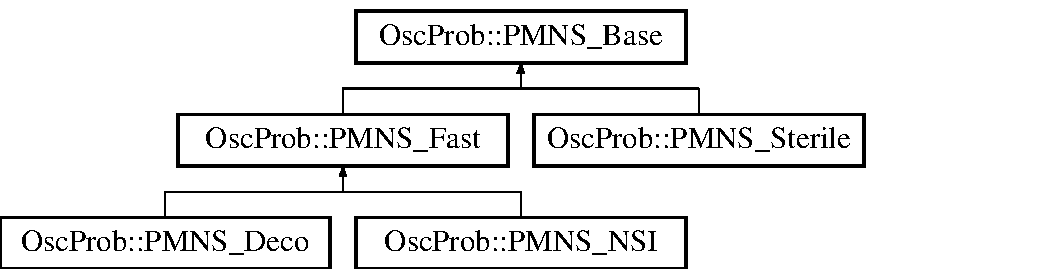
\includegraphics[height=3.000000cm]{classOscProb_1_1PMNS__Base}
\end{center}
\end{figure}
\subsection*{Public Types}
\begin{DoxyCompactItemize}
\item 
typedef std\+::complex$<$ double $>$ \hyperlink{classOscProb_1_1PMNS__Base_ae86ec4718808ce9d02e5f5b4226714ab}{complex}
\end{DoxyCompactItemize}
\subsection*{Public Member Functions}
\begin{DoxyCompactItemize}
\item 
\hyperlink{classOscProb_1_1PMNS__Base_aa53e83b03a9cf4bdfa0a07136bd17a79}{P\+M\+N\+S\+\_\+\+Base} (int num\+Nus=3)
\begin{DoxyCompactList}\small\item\em Constructor. \end{DoxyCompactList}\item 
virtual \hyperlink{classOscProb_1_1PMNS__Base_a91223a852214dd90da9b4403f779dbbf}{$\sim$\+P\+M\+N\+S\+\_\+\+Base} ()
\begin{DoxyCompactList}\small\item\em Destructor. \end{DoxyCompactList}\item 
virtual double \hyperlink{classOscProb_1_1PMNS__Base_aec5c399b93261f1962a4b7dbbb44b973}{Prob} (int flvi, int flvf)
\begin{DoxyCompactList}\small\item\em Compute the probability of flvi going to flvf. \end{DoxyCompactList}\item 
virtual double \hyperlink{classOscProb_1_1PMNS__Base_aa3cee10639d5c0879ccb9e78d62128d3}{Prob} (int flvi, int flvf, double E)
\begin{DoxyCompactList}\small\item\em Compute the probability of flvi going to flvf for energy E. \end{DoxyCompactList}\item 
virtual double \hyperlink{classOscProb_1_1PMNS__Base_a6e0a74508d9d6db7be02e242b8467563}{Prob} (int flvi, int flvf, double E, double L)
\begin{DoxyCompactList}\small\item\em Compute the probability of flvi going to flvf for energy E and distance L. \end{DoxyCompactList}\item 
virtual double \hyperlink{classOscProb_1_1PMNS__Base_ac03f754160422e6600da8dbae0f803ed}{Avg\+Prob} (int flvi, int flvf, double E, double dE=0)
\begin{DoxyCompactList}\small\item\em Compute the average probability over a bin of energy. \end{DoxyCompactList}\item 
virtual double \hyperlink{classOscProb_1_1PMNS__Base_ac19a92f4ef428a7333ca8eed76fca637}{Avg\+Prob\+LoE} (int flvi, int flvf, double LoE, double d\+LoE=0)
\begin{DoxyCompactList}\small\item\em Compute the average probability over a bin of L/E. \end{DoxyCompactList}\item 
virtual void \hyperlink{classOscProb_1_1PMNS__Base_ace7875cf6d3bec161a2b7ed2690aec34}{Set\+Angle} (int i, int j, double th)
\begin{DoxyCompactList}\small\item\em Set the mixing angle theta\+\_\+ij. \end{DoxyCompactList}\item 
virtual void \hyperlink{classOscProb_1_1PMNS__Base_a4bef78cfcfc4e70b4ce79cdb8862c0a3}{Set\+Delta} (int i, int j, double delta)
\begin{DoxyCompactList}\small\item\em Set the CP phase delta\+\_\+ij. \end{DoxyCompactList}\item 
virtual void \hyperlink{classOscProb_1_1PMNS__Base_a492243b22fb1b783cd2943f507cff970}{Set\+Dm} (int j, double dm)
\begin{DoxyCompactList}\small\item\em Set the mass-\/splitting dm\+\_\+j1 in e\+V$^\wedge$2. \end{DoxyCompactList}\item 
virtual double \hyperlink{classOscProb_1_1PMNS__Base_acee137091304c919642293ddf015bbc8}{Get\+Angle} (int i, int j)
\begin{DoxyCompactList}\small\item\em Get the mixing angle theta\+\_\+ij. \end{DoxyCompactList}\item 
virtual double \hyperlink{classOscProb_1_1PMNS__Base_adb8dbc91d4286d2e7c8f768c59476241}{Get\+Delta} (int i, int j)
\begin{DoxyCompactList}\small\item\em Get the CP phase delta\+\_\+ij. \end{DoxyCompactList}\item 
virtual double \hyperlink{classOscProb_1_1PMNS__Base_ad26815ac5f4805d1259817e4936e5f8f}{Get\+Dm} (int j)
\begin{DoxyCompactList}\small\item\em Get the mass-\/splitting dm\+\_\+j1 in e\+V$^\wedge$2. \end{DoxyCompactList}\item 
virtual void \hyperlink{classOscProb_1_1PMNS__Base_a4de96ac9b6d1e9b029ab877e57d211ad}{Set\+Std\+Pars} ()
\begin{DoxyCompactList}\small\item\em Set P\+DG 3-\/flavor parameters. \end{DoxyCompactList}\item 
virtual void \hyperlink{classOscProb_1_1PMNS__Base_a95b3b0d0cab5e6a54b5ef99587f837c0}{Set\+Energy} (double E)
\begin{DoxyCompactList}\small\item\em Set the neutrino energy in GeV. \end{DoxyCompactList}\item 
virtual void \hyperlink{classOscProb_1_1PMNS__Base_a717e0348cf762f3961854e332a9b52e0}{Set\+Is\+Nu\+Bar} (bool is\+Nu\+Bar)
\begin{DoxyCompactList}\small\item\em Set the anti-\/neutrino flag. \end{DoxyCompactList}\item 
virtual double \hyperlink{classOscProb_1_1PMNS__Base_acc0d46cc4b8f911b40b807225003bbed}{Get\+Energy} ()
\begin{DoxyCompactList}\small\item\em Get the neutrino energy in GeV. \end{DoxyCompactList}\item 
virtual bool \hyperlink{classOscProb_1_1PMNS__Base_a2f7f2a028dfe7a90fff6b4f757972c2c}{Get\+Is\+Nu\+Bar} ()
\begin{DoxyCompactList}\small\item\em Get the anti-\/neutrino flag. \end{DoxyCompactList}\item 
virtual void \hyperlink{classOscProb_1_1PMNS__Base_ac3b644fd0a56347d304ceca4ae9d8875}{Set\+Path} (\hyperlink{structOscProb_1_1NuPath}{Osc\+Prob\+::\+Nu\+Path} p)
\begin{DoxyCompactList}\small\item\em Set a single path. \end{DoxyCompactList}\item 
virtual void \hyperlink{classOscProb_1_1PMNS__Base_a35b983270613072a3df58b574d80dbfd}{Set\+Path} (double length, double density, double zoa=0.\+5, int layer=0)
\begin{DoxyCompactList}\small\item\em Set a single path. \end{DoxyCompactList}\item 
virtual void \hyperlink{classOscProb_1_1PMNS__Base_a0182eaef7655e85b17738ea0cd5f7cad}{Set\+Path} (vector$<$ \hyperlink{structOscProb_1_1NuPath}{Osc\+Prob\+::\+Nu\+Path} $>$ paths)
\begin{DoxyCompactList}\small\item\em Set a path sequence. \end{DoxyCompactList}\item 
virtual void \hyperlink{classOscProb_1_1PMNS__Base_a887dc9d4dc569ec0cdef3933b4c60efc}{Add\+Path} (\hyperlink{structOscProb_1_1NuPath}{Osc\+Prob\+::\+Nu\+Path} p)
\begin{DoxyCompactList}\small\item\em Add a path to the sequence. \end{DoxyCompactList}\item 
virtual void \hyperlink{classOscProb_1_1PMNS__Base_ab7f89ad9e7e1224adaa59d3c41594cd9}{Add\+Path} (double length, double density, double zoa=0.\+5, int layer=0)
\begin{DoxyCompactList}\small\item\em Add a path to the sequence. \end{DoxyCompactList}\item 
virtual void \hyperlink{classOscProb_1_1PMNS__Base_aefe521239031c418cfaaaa550a6e13bb}{Clear\+Path} ()
\begin{DoxyCompactList}\small\item\em Clear the path vector. \end{DoxyCompactList}\item 
virtual void \hyperlink{classOscProb_1_1PMNS__Base_a6241325b1bd28cafa556daaecbe4ed62}{Set\+Length} (double L)
\begin{DoxyCompactList}\small\item\em Set a single path lentgh in km. \end{DoxyCompactList}\item 
virtual void \hyperlink{classOscProb_1_1PMNS__Base_ac74206f349687da141392c81e2ba6b0d}{Set\+Density} (double rho)
\begin{DoxyCompactList}\small\item\em Set single path density in g/cm$^\wedge$3. \end{DoxyCompactList}\item 
virtual void \hyperlink{classOscProb_1_1PMNS__Base_a1bf3ea8fd2507fd2fd82d7410ff8f578}{Set\+ZoA} (double zoa)
\begin{DoxyCompactList}\small\item\em Set Z/A value for single path. \end{DoxyCompactList}\item 
virtual void \hyperlink{classOscProb_1_1PMNS__Base_a6c45d94d421a63d7de98b641596b0439}{Set\+Length} (vector$<$ double $>$ L)
\begin{DoxyCompactList}\small\item\em Set multiple path lengths. \end{DoxyCompactList}\item 
virtual void \hyperlink{classOscProb_1_1PMNS__Base_adacda3e7ff4527419eb0444cd47dfc94}{Set\+Density} (vector$<$ double $>$ rho)
\begin{DoxyCompactList}\small\item\em Set multiple path densities. \end{DoxyCompactList}\item 
virtual void \hyperlink{classOscProb_1_1PMNS__Base_a7d5824ef701980cf8728794b7331d8ae}{Set\+ZoA} (vector$<$ double $>$ zoa)
\begin{DoxyCompactList}\small\item\em Set multiple path Z/A values. \end{DoxyCompactList}\item 
virtual void \hyperlink{classOscProb_1_1PMNS__Base_a9aaeae28c7ba42686fb0027301882b07}{Set\+Layers} (vector$<$ int $>$ lay)
\begin{DoxyCompactList}\small\item\em Set multiple path layer indices. \end{DoxyCompactList}\item 
virtual void \hyperlink{classOscProb_1_1PMNS__Base_add6533a9fc9acdfc7ae258b62570d78d}{Set\+Std\+Path} ()
\begin{DoxyCompactList}\small\item\em Set standard neutrino path. \end{DoxyCompactList}\item 
virtual vector$<$ \hyperlink{structOscProb_1_1NuPath}{Osc\+Prob\+::\+Nu\+Path} $>$ \hyperlink{classOscProb_1_1PMNS__Base_ac8e196f2e85a2b1caaf705073ee95a5c}{Get\+Path} ()
\begin{DoxyCompactList}\small\item\em Get the neutrino path sequence. \end{DoxyCompactList}\item 
virtual vector$<$ double $>$ \hyperlink{classOscProb_1_1PMNS__Base_a9eac8d768c1424755ee41f7e783af179}{Get\+Sample\+Points} (double LoE, double d\+LoE)
\begin{DoxyCompactList}\small\item\em Compute the sample points for a bin of L/E with width d\+LoE. \end{DoxyCompactList}\end{DoxyCompactItemize}
\subsection*{Protected Member Functions}
\begin{DoxyCompactItemize}
\item 
virtual void \hyperlink{classOscProb_1_1PMNS__Base_adf23b569112f9f9e0e592f01d79a5f3d}{Initialize\+Vectors} ()
\begin{DoxyCompactList}\small\item\em Initialize all member vectors with zeros. \end{DoxyCompactList}\item 
virtual void \hyperlink{classOscProb_1_1PMNS__Base_a986e6ebef09a7e2eb7fee16a4c2c834d}{Set\+Cur\+Path} (\hyperlink{structOscProb_1_1NuPath}{Osc\+Prob\+::\+Nu\+Path} p)
\begin{DoxyCompactList}\small\item\em Set the path currently in use by the class. \end{DoxyCompactList}\item 
virtual void \hyperlink{classOscProb_1_1PMNS__Base_aba565962a440d14bee7a2a96d2eca2c5}{Set\+Att} (double att, int idx)
\begin{DoxyCompactList}\small\item\em Set one of the path attributes. \end{DoxyCompactList}\item 
virtual void \hyperlink{classOscProb_1_1PMNS__Base_afdd763ad1ad643443775776efc73660b}{Set\+Att} (vector$<$ double $>$ att, int idx)
\begin{DoxyCompactList}\small\item\em Set all values of a path attribute. \end{DoxyCompactList}\item 
virtual void \hyperlink{classOscProb_1_1PMNS__Base_aae18afd69074211335f49ec40e6011b9}{RotateH} (int i, int j)
\begin{DoxyCompactList}\small\item\em Rotate the Hamiltonian by theta\+\_\+ij and delta\+\_\+ij. \end{DoxyCompactList}\item 
virtual void \hyperlink{classOscProb_1_1PMNS__Base_ad0faf5eae755afb1baa1fcd5ffebad41}{Build\+Hms} ()
\begin{DoxyCompactList}\small\item\em Build the matrix of masses squared. \end{DoxyCompactList}\item 
virtual void \hyperlink{classOscProb_1_1PMNS__Base_a91f065cb9e910e0095e41462b4420b01}{Solve\+Ham} ()=0
\begin{DoxyCompactList}\small\item\em Solve the full Hamiltonian for eigenvectors and eigenvalues. \end{DoxyCompactList}\item 
virtual void \hyperlink{classOscProb_1_1PMNS__Base_ac0d4bf8ff1318ef96d3dafa62e0cec25}{Reset\+To\+Flavour} (int flv)
\begin{DoxyCompactList}\small\item\em Reset neutrino state to pure flavour flv. \end{DoxyCompactList}\item 
virtual void \hyperlink{classOscProb_1_1PMNS__Base_accb08503acc162188041d7a96a280462}{Propagate\+Path} (\hyperlink{structOscProb_1_1NuPath}{Osc\+Prob\+::\+Nu\+Path} p)
\begin{DoxyCompactList}\small\item\em Propagate neutrino through a single path. \end{DoxyCompactList}\item 
virtual void \hyperlink{classOscProb_1_1PMNS__Base_a054e3a8b05b9a958b6fa416e4a835e3e}{Propagate} ()
\begin{DoxyCompactList}\small\item\em Propagate neutrino through full path. \end{DoxyCompactList}\item 
virtual double \hyperlink{classOscProb_1_1PMNS__Base_a0dc4d45bc3d7e03b9abbf5b4e100cc22}{P} (int flv)
\begin{DoxyCompactList}\small\item\em Return the probability of final state in flavour flv. \end{DoxyCompactList}\end{DoxyCompactItemize}
\subsection*{Protected Attributes}
\begin{DoxyCompactItemize}
\item 
int \hyperlink{classOscProb_1_1PMNS__Base_a24bb74bed63569dfe88b18fa6a08060e}{f\+Num\+Nus}
\begin{DoxyCompactList}\small\item\em Number of neutrino flavours. \end{DoxyCompactList}\item 
vector$<$ double $>$ \hyperlink{classOscProb_1_1PMNS__Base_af334c4deea47a6da3a7b56cb065dd33a}{f\+Dm}
\begin{DoxyCompactList}\small\item\em m$^\wedge$2\+\_\+i -\/ m$^\wedge$2\+\_\+1 in vacuum \end{DoxyCompactList}\item 
vector$<$ vector$<$ double $>$ $>$ \hyperlink{classOscProb_1_1PMNS__Base_ad0183329d415e6f38c07d996f5d3a386}{f\+Theta}
\begin{DoxyCompactList}\small\item\em theta\mbox{[}i\mbox{]}\mbox{[}j\mbox{]} mixing angle \end{DoxyCompactList}\item 
vector$<$ vector$<$ double $>$ $>$ \hyperlink{classOscProb_1_1PMNS__Base_a11a921aae83652158798b03b89c02d02}{f\+Delta}
\begin{DoxyCompactList}\small\item\em delta\mbox{[}i\mbox{]}\mbox{[}j\mbox{]} CP violating phase \end{DoxyCompactList}\item 
vector$<$ \hyperlink{classOscProb_1_1PMNS__Base_ae86ec4718808ce9d02e5f5b4226714ab}{complex} $>$ \hyperlink{classOscProb_1_1PMNS__Base_a381f188a7742a4b3e4aa049dd3701af0}{f\+Nu\+State}
\begin{DoxyCompactList}\small\item\em The neutrino current state. \end{DoxyCompactList}\item 
vector$<$ vector$<$ \hyperlink{classOscProb_1_1PMNS__Base_ae86ec4718808ce9d02e5f5b4226714ab}{complex} $>$ $>$ \hyperlink{classOscProb_1_1PMNS__Base_aacf4949fc2c9cbc038e8a22af9665283}{f\+Hms}
\begin{DoxyCompactList}\small\item\em matrix H$\ast$2E in e\+V$^\wedge$2 \end{DoxyCompactList}\item 
vector$<$ double $>$ \hyperlink{classOscProb_1_1PMNS__Base_af21567a38b244621747ab56f9b550962}{f\+Eval}
\begin{DoxyCompactList}\small\item\em Eigenvalues of the Hamiltonian. \end{DoxyCompactList}\item 
vector$<$ vector$<$ \hyperlink{classOscProb_1_1PMNS__Base_ae86ec4718808ce9d02e5f5b4226714ab}{complex} $>$ $>$ \hyperlink{classOscProb_1_1PMNS__Base_a2b6db9376045dd88a66f8e5f06b2f6a9}{f\+Evec}
\begin{DoxyCompactList}\small\item\em Eigenvectors of the Hamiltonian. \end{DoxyCompactList}\item 
double \hyperlink{classOscProb_1_1PMNS__Base_a2800af6d436972f3e900867790c046b0}{f\+Energy}
\begin{DoxyCompactList}\small\item\em Neutrino energy. \end{DoxyCompactList}\item 
bool \hyperlink{classOscProb_1_1PMNS__Base_a0ebaeaefab36a3ff381c6293faedfdd6}{f\+Is\+Nu\+Bar}
\begin{DoxyCompactList}\small\item\em Anti-\/neutrino flag. \end{DoxyCompactList}\item 
vector$<$ \hyperlink{structOscProb_1_1NuPath}{Osc\+Prob\+::\+Nu\+Path} $>$ \hyperlink{classOscProb_1_1PMNS__Base_a0bbaf35114db6c74e37c810947219558}{f\+Nu\+Paths}
\begin{DoxyCompactList}\small\item\em Vector of neutrino paths. \end{DoxyCompactList}\item 
\hyperlink{structOscProb_1_1NuPath}{Osc\+Prob\+::\+Nu\+Path} \hyperlink{classOscProb_1_1PMNS__Base_a849437aa8891fe042e86886ce8f81c6e}{f\+Path}
\begin{DoxyCompactList}\small\item\em Current neutrino path. \end{DoxyCompactList}\item 
bool \hyperlink{classOscProb_1_1PMNS__Base_a9ac3cadeac8db1b90f3152f476244780}{f\+Built\+Hms}
\begin{DoxyCompactList}\small\item\em Tag to avoid rebuilding Hms. \end{DoxyCompactList}\item 
bool \hyperlink{classOscProb_1_1PMNS__Base_a6dc5cd010d2d70b2324745b4e53e9839}{f\+Got\+ES}
\begin{DoxyCompactList}\small\item\em Tag to avoid recalculating eigensystem. \end{DoxyCompactList}\end{DoxyCompactItemize}
\subsection*{Static Protected Attributes}
\begin{DoxyCompactItemize}
\item 
static const \hyperlink{classOscProb_1_1PMNS__Base_ae86ec4718808ce9d02e5f5b4226714ab}{complex} \hyperlink{classOscProb_1_1PMNS__Base_a5c31ed4593cf95feb36fb80c1850d25e}{zero}
\begin{DoxyCompactList}\small\item\em zero in complex \end{DoxyCompactList}\item 
static const \hyperlink{classOscProb_1_1PMNS__Base_ae86ec4718808ce9d02e5f5b4226714ab}{complex} \hyperlink{classOscProb_1_1PMNS__Base_ab64aab27448a5aca27565c991a9d173e}{one}
\begin{DoxyCompactList}\small\item\em one in complex \end{DoxyCompactList}\item 
static const double \hyperlink{classOscProb_1_1PMNS__Base_a382ddd7b76ca89b43f22614a2ea7327b}{k\+Km2eV} = 1.\+0 / 1.\+973269718e-\/10
\begin{DoxyCompactList}\small\item\em km to e\+V$^\wedge$-\/1 \end{DoxyCompactList}\item 
static const double \hyperlink{classOscProb_1_1PMNS__Base_a326fc5016d7dd7ce05682c06cdcb6d94}{k\+K2} = 4.\+62711501e-\/09
\begin{DoxyCompactList}\small\item\em mol/\+Ge\+V$^\wedge$2/cm$^\wedge$3 to eV \end{DoxyCompactList}\item 
static const double \hyperlink{classOscProb_1_1PMNS__Base_ad36a0a6bf58d6ec093d3947784bd89e9}{k\+Ge\+V2eV} = 1.\+0e+09
\begin{DoxyCompactList}\small\item\em GeV to eV. \end{DoxyCompactList}\item 
static const double \hyperlink{classOscProb_1_1PMNS__Base_a7f26a3456128234b2ae6cc9141a6532f}{k\+Gf} = 1.\+1663787e-\/05
\begin{DoxyCompactList}\small\item\em G\+\_\+F in units of Ge\+V$^\wedge$-\/2. \end{DoxyCompactList}\end{DoxyCompactItemize}


\subsection{Detailed Description}
This is an abstract class implementing the general functions needed for setting up an oscillation calculator. The method for solving the eigensystem for the Hamiltonian must be defined in the derived classes.

\begin{DoxySeeAlso}{See also}
\hyperlink{classOscProb_1_1PMNS__Fast}{P\+M\+N\+S\+\_\+\+Fast} \hyperlink{classOscProb_1_1PMNS__NSI}{P\+M\+N\+S\+\_\+\+N\+SI} \hyperlink{classOscProb_1_1PMNS__Sterile}{P\+M\+N\+S\+\_\+\+Sterile}
\end{DoxySeeAlso}
\begin{DoxyAuthor}{Author}
Joao Coelho -\/ jcoelho@apc.\+in2p3.\+fr 
\end{DoxyAuthor}


Definition at line 27 of file P\+M\+N\+S\+\_\+\+Base.\+h.



\subsection{Member Typedef Documentation}
\index{Osc\+Prob\+::\+P\+M\+N\+S\+\_\+\+Base@{Osc\+Prob\+::\+P\+M\+N\+S\+\_\+\+Base}!complex@{complex}}
\index{complex@{complex}!Osc\+Prob\+::\+P\+M\+N\+S\+\_\+\+Base@{Osc\+Prob\+::\+P\+M\+N\+S\+\_\+\+Base}}
\subsubsection[{\texorpdfstring{complex}{complex}}]{\setlength{\rightskip}{0pt plus 5cm}typedef std\+::complex$<$double$>$ {\bf Osc\+Prob\+::\+P\+M\+N\+S\+\_\+\+Base\+::complex}}\hypertarget{classOscProb_1_1PMNS__Base_ae86ec4718808ce9d02e5f5b4226714ab}{}\label{classOscProb_1_1PMNS__Base_ae86ec4718808ce9d02e5f5b4226714ab}


Definition at line 107 of file P\+M\+N\+S\+\_\+\+Base.\+h.



\subsection{Constructor \& Destructor Documentation}
\index{Osc\+Prob\+::\+P\+M\+N\+S\+\_\+\+Base@{Osc\+Prob\+::\+P\+M\+N\+S\+\_\+\+Base}!P\+M\+N\+S\+\_\+\+Base@{P\+M\+N\+S\+\_\+\+Base}}
\index{P\+M\+N\+S\+\_\+\+Base@{P\+M\+N\+S\+\_\+\+Base}!Osc\+Prob\+::\+P\+M\+N\+S\+\_\+\+Base@{Osc\+Prob\+::\+P\+M\+N\+S\+\_\+\+Base}}
\subsubsection[{\texorpdfstring{P\+M\+N\+S\+\_\+\+Base(int num\+Nus=3)}{PMNS_Base(int numNus=3)}}]{\setlength{\rightskip}{0pt plus 5cm}P\+M\+N\+S\+\_\+\+Base\+::\+P\+M\+N\+S\+\_\+\+Base (
\begin{DoxyParamCaption}
\item[{int}]{num\+Nus = {\ttfamily 3}}
\end{DoxyParamCaption}
)}\hypertarget{classOscProb_1_1PMNS__Base_aa53e83b03a9cf4bdfa0a07136bd17a79}{}\label{classOscProb_1_1PMNS__Base_aa53e83b03a9cf4bdfa0a07136bd17a79}
Constructor.

Sets the number of neutrinos and initializes attributes

Default starts with a 2 GeV muon neutrino.

Path is set to the default 1000 km in crust density.

Oscillation parameters are from P\+DG for NH by default.


\begin{DoxyParams}{Parameters}
{\em num\+Nus} & -\/ the number of neutrino flavours \\
\hline
\end{DoxyParams}


Definition at line 47 of file P\+M\+N\+S\+\_\+\+Base.\+cxx.



References f\+Num\+Nus, Initialize\+Vectors(), Reset\+To\+Flavour(), Set\+Energy(), Set\+Is\+Nu\+Bar(), Set\+Std\+Pars(), and Set\+Std\+Path().


\begin{DoxyCode}
47                                :
48 \hyperlink{classOscProb_1_1PMNS__Base_a6dc5cd010d2d70b2324745b4e53e9839}{fGotES}(\textcolor{keyword}{false}), \hyperlink{classOscProb_1_1PMNS__Base_a9ac3cadeac8db1b90f3152f476244780}{fBuiltHms}(\textcolor{keyword}{false})
49 \{
50 
51   \hyperlink{classOscProb_1_1PMNS__Base_a24bb74bed63569dfe88b18fa6a08060e}{fNumNus} = numNus;    \textcolor{comment}{// Set the number of neutrinos}
52 
53   \hyperlink{classOscProb_1_1PMNS__Base_add6533a9fc9acdfc7ae258b62570d78d}{SetStdPath}();        \textcolor{comment}{// Set some default path}
54   \hyperlink{classOscProb_1_1PMNS__Base_a95b3b0d0cab5e6a54b5ef99587f837c0}{SetEnergy}(2);        \textcolor{comment}{// Set default energy to 2 GeV}
55   \hyperlink{classOscProb_1_1PMNS__Base_a717e0348cf762f3961854e332a9b52e0}{SetIsNuBar}(\textcolor{keyword}{false});   \textcolor{comment}{// Neutrino by default}
56 
57   \hyperlink{classOscProb_1_1PMNS__Base_adf23b569112f9f9e0e592f01d79a5f3d}{InitializeVectors}(); \textcolor{comment}{// Initialize all vectors}
58 
59   \hyperlink{classOscProb_1_1PMNS__Base_a4de96ac9b6d1e9b029ab877e57d211ad}{SetStdPars}();        \textcolor{comment}{// Set PDG parameters}
60 
61   \hyperlink{classOscProb_1_1PMNS__Base_ac0d4bf8ff1318ef96d3dafa62e0cec25}{ResetToFlavour}(1);   \textcolor{comment}{// Numu by default}
62 
63 \}
\end{DoxyCode}
\index{Osc\+Prob\+::\+P\+M\+N\+S\+\_\+\+Base@{Osc\+Prob\+::\+P\+M\+N\+S\+\_\+\+Base}!````~P\+M\+N\+S\+\_\+\+Base@{$\sim$\+P\+M\+N\+S\+\_\+\+Base}}
\index{````~P\+M\+N\+S\+\_\+\+Base@{$\sim$\+P\+M\+N\+S\+\_\+\+Base}!Osc\+Prob\+::\+P\+M\+N\+S\+\_\+\+Base@{Osc\+Prob\+::\+P\+M\+N\+S\+\_\+\+Base}}
\subsubsection[{\texorpdfstring{$\sim$\+P\+M\+N\+S\+\_\+\+Base()}{~PMNS_Base()}}]{\setlength{\rightskip}{0pt plus 5cm}P\+M\+N\+S\+\_\+\+Base\+::$\sim$\+P\+M\+N\+S\+\_\+\+Base (
\begin{DoxyParamCaption}
{}
\end{DoxyParamCaption}
)\hspace{0.3cm}{\ttfamily [virtual]}}\hypertarget{classOscProb_1_1PMNS__Base_a91223a852214dd90da9b4403f779dbbf}{}\label{classOscProb_1_1PMNS__Base_a91223a852214dd90da9b4403f779dbbf}
Nothing to clean. 

Definition at line 69 of file P\+M\+N\+S\+\_\+\+Base.\+cxx.


\begin{DoxyCode}
69 \{\}
\end{DoxyCode}


\subsection{Member Function Documentation}
\index{Osc\+Prob\+::\+P\+M\+N\+S\+\_\+\+Base@{Osc\+Prob\+::\+P\+M\+N\+S\+\_\+\+Base}!Add\+Path@{Add\+Path}}
\index{Add\+Path@{Add\+Path}!Osc\+Prob\+::\+P\+M\+N\+S\+\_\+\+Base@{Osc\+Prob\+::\+P\+M\+N\+S\+\_\+\+Base}}
\subsubsection[{\texorpdfstring{Add\+Path(\+Osc\+Prob\+::\+Nu\+Path p)}{AddPath(OscProb::NuPath p)}}]{\setlength{\rightskip}{0pt plus 5cm}void P\+M\+N\+S\+\_\+\+Base\+::\+Add\+Path (
\begin{DoxyParamCaption}
\item[{{\bf Osc\+Prob\+::\+Nu\+Path}}]{p}
\end{DoxyParamCaption}
)\hspace{0.3cm}{\ttfamily [virtual]}}\hypertarget{classOscProb_1_1PMNS__Base_a887dc9d4dc569ec0cdef3933b4c60efc}{}\label{classOscProb_1_1PMNS__Base_a887dc9d4dc569ec0cdef3933b4c60efc}
Add a path to the sequence. 
\begin{DoxyParams}{Parameters}
{\em p} & -\/ A neutrino path segment \\
\hline
\end{DoxyParams}


Definition at line 256 of file P\+M\+N\+S\+\_\+\+Base.\+cxx.



References f\+Nu\+Paths.



Referenced by Add\+Path(), Set\+Att(), and Set\+Path().


\begin{DoxyCode}
256                                \{
257 
258   \hyperlink{classOscProb_1_1PMNS__Base_a0bbaf35114db6c74e37c810947219558}{fNuPaths}.push\_back(p);
259 
260 \}
\end{DoxyCode}
\index{Osc\+Prob\+::\+P\+M\+N\+S\+\_\+\+Base@{Osc\+Prob\+::\+P\+M\+N\+S\+\_\+\+Base}!Add\+Path@{Add\+Path}}
\index{Add\+Path@{Add\+Path}!Osc\+Prob\+::\+P\+M\+N\+S\+\_\+\+Base@{Osc\+Prob\+::\+P\+M\+N\+S\+\_\+\+Base}}
\subsubsection[{\texorpdfstring{Add\+Path(double length, double density, double zoa=0.\+5, int layer=0)}{AddPath(double length, double density, double zoa=0.5, int layer=0)}}]{\setlength{\rightskip}{0pt plus 5cm}void P\+M\+N\+S\+\_\+\+Base\+::\+Add\+Path (
\begin{DoxyParamCaption}
\item[{double}]{length, }
\item[{double}]{density, }
\item[{double}]{zoa = {\ttfamily 0.5}, }
\item[{int}]{layer = {\ttfamily 0}}
\end{DoxyParamCaption}
)\hspace{0.3cm}{\ttfamily [virtual]}}\hypertarget{classOscProb_1_1PMNS__Base_ab7f89ad9e7e1224adaa59d3c41594cd9}{}\label{classOscProb_1_1PMNS__Base_ab7f89ad9e7e1224adaa59d3c41594cd9}
Add a path to the sequence defining attributes directly. 
\begin{DoxyParams}{Parameters}
{\em length} & -\/ The length of the path segment in km \\
\hline
{\em density} & -\/ The density of the path segment in g/cm$^\wedge$3 \\
\hline
{\em zoa} & -\/ The effective Z/A of the path segment \\
\hline
{\em layer} & -\/ An index to identify the layer type (e.\+g. earth inner core) \\
\hline
\end{DoxyParams}


Definition at line 270 of file P\+M\+N\+S\+\_\+\+Base.\+cxx.



References Add\+Path().


\begin{DoxyCode}
270                                                                            \{
271 
272   \hyperlink{classOscProb_1_1PMNS__Base_a887dc9d4dc569ec0cdef3933b4c60efc}{AddPath}(\hyperlink{structOscProb_1_1NuPath}{NuPath}(length, density, zoa, layer));
273 
274 \}
\end{DoxyCode}
\index{Osc\+Prob\+::\+P\+M\+N\+S\+\_\+\+Base@{Osc\+Prob\+::\+P\+M\+N\+S\+\_\+\+Base}!Avg\+Prob@{Avg\+Prob}}
\index{Avg\+Prob@{Avg\+Prob}!Osc\+Prob\+::\+P\+M\+N\+S\+\_\+\+Base@{Osc\+Prob\+::\+P\+M\+N\+S\+\_\+\+Base}}
\subsubsection[{\texorpdfstring{Avg\+Prob(int flvi, int flvf, double E, double d\+E=0)}{AvgProb(int flvi, int flvf, double E, double dE=0)}}]{\setlength{\rightskip}{0pt plus 5cm}double P\+M\+N\+S\+\_\+\+Base\+::\+Avg\+Prob (
\begin{DoxyParamCaption}
\item[{int}]{flvi, }
\item[{int}]{flvf, }
\item[{double}]{E, }
\item[{double}]{dE = {\ttfamily 0}}
\end{DoxyParamCaption}
)\hspace{0.3cm}{\ttfamily [virtual]}}\hypertarget{classOscProb_1_1PMNS__Base_ac03f754160422e6600da8dbae0f803ed}{}\label{classOscProb_1_1PMNS__Base_ac03f754160422e6600da8dbae0f803ed}
Compute the average probability of flvi going to flvf over a bin of energy E with width dE.

This gets transformed into L/E, since the oscillation terms have arguments linear in L/E and not E.

This function currently only works for single paths.

Flavours are\+: 
\begin{DoxyPre}
  0 = nue, 1 = numu, 2 = nutau
  3 = sterile\_1, 4 = sterile\_2, etc.
\end{DoxyPre}
 
\begin{DoxyParams}{Parameters}
{\em flvi} & -\/ The neutrino starting flavour. \\
\hline
{\em flvf} & -\/ The neutrino final flavour. \\
\hline
{\em E} & -\/ The neutrino energy in the bin center in GeV \\
\hline
{\em dE} & -\/ The energy bin width in GeV\\
\hline
\end{DoxyParams}
\begin{DoxyReturn}{Returns}
Average neutrino oscillation probability 
\end{DoxyReturn}


Definition at line 1076 of file P\+M\+N\+S\+\_\+\+Base.\+cxx.



References Avg\+Prob\+Lo\+E(), f\+Nu\+Paths, f\+Path, Osc\+Prob\+::\+Nu\+Path\+::length, Prob(), and Set\+Cur\+Path().


\begin{DoxyCode}
1077 \{
1078 
1079   \textcolor{comment}{// Do nothing if energy is not positive}
1080   \textcolor{keywordflow}{if}(E<=0) \textcolor{keywordflow}{return} 0;
1081 
1082   \textcolor{keywordflow}{if}(\hyperlink{classOscProb_1_1PMNS__Base_a0bbaf35114db6c74e37c810947219558}{fNuPaths}.empty()) \textcolor{keywordflow}{return} 0;
1083 
1084   \textcolor{keywordflow}{if}(\hyperlink{classOscProb_1_1PMNS__Base_a0bbaf35114db6c74e37c810947219558}{fNuPaths}.size() != 1)\{
1085     cout << \textcolor{stringliteral}{"ERROR: AvgProb not implemented for multiple paths."} << endl;
1086     cout << \textcolor{stringliteral}{"       Returning probability at bin center."} << endl;
1087     \textcolor{keywordflow}{return} \hyperlink{classOscProb_1_1PMNS__Base_aec5c399b93261f1962a4b7dbbb44b973}{Prob}(flvi, flvf, E);
1088   \}
1089 
1090   \textcolor{comment}{// Don't average zero width}
1091   \textcolor{keywordflow}{if}(dE<=0) \textcolor{keywordflow}{return} \hyperlink{classOscProb_1_1PMNS__Base_aec5c399b93261f1962a4b7dbbb44b973}{Prob}(flvi, flvf, E);
1092 
1093   \textcolor{comment}{// Make sure fPath is set}
1094   \hyperlink{classOscProb_1_1PMNS__Base_a986e6ebef09a7e2eb7fee16a4c2c834d}{SetCurPath}(\hyperlink{classOscProb_1_1PMNS__Base_a0bbaf35114db6c74e37c810947219558}{fNuPaths}[0]);
1095 
1096   \textcolor{comment}{// Define L/E variables}
1097   \textcolor{keywordtype}{double} LoE = 0;
1098   \textcolor{keywordtype}{double} dLoE = 0;
1099 
1100   \textcolor{comment}{// Set a minimum energy}
1101   \textcolor{keywordtype}{double} minE = 0.1 * E;
1102 
1103   \textcolor{comment}{// Transform range to L/E}
1104   \textcolor{comment}{// Full range if low edge > minE}
1105   \textcolor{keywordflow}{if}(E-dE/2 > minE)\{
1106     LoE = 0.5 * (\hyperlink{classOscProb_1_1PMNS__Base_a849437aa8891fe042e86886ce8f81c6e}{fPath}.\hyperlink{structOscProb_1_1NuPath_af22660894b6e25cf835500381b155557}{length}/(E-dE/2) + \hyperlink{classOscProb_1_1PMNS__Base_a849437aa8891fe042e86886ce8f81c6e}{fPath}.\hyperlink{structOscProb_1_1NuPath_af22660894b6e25cf835500381b155557}{length}/(E+dE/2));
1107     dLoE = \hyperlink{classOscProb_1_1PMNS__Base_a849437aa8891fe042e86886ce8f81c6e}{fPath}.\hyperlink{structOscProb_1_1NuPath_af22660894b6e25cf835500381b155557}{length}/(E-dE/2) - \hyperlink{classOscProb_1_1PMNS__Base_a849437aa8891fe042e86886ce8f81c6e}{fPath}.\hyperlink{structOscProb_1_1NuPath_af22660894b6e25cf835500381b155557}{length}/(E+dE/2);
1108   \}
1109   \textcolor{comment}{// Else start at minE}
1110   \textcolor{keywordflow}{else}\{
1111     LoE = 0.5 * (\hyperlink{classOscProb_1_1PMNS__Base_a849437aa8891fe042e86886ce8f81c6e}{fPath}.\hyperlink{structOscProb_1_1NuPath_af22660894b6e25cf835500381b155557}{length}/minE + \hyperlink{classOscProb_1_1PMNS__Base_a849437aa8891fe042e86886ce8f81c6e}{fPath}.\hyperlink{structOscProb_1_1NuPath_af22660894b6e25cf835500381b155557}{length}/(E+dE/2));
1112     dLoE = \hyperlink{classOscProb_1_1PMNS__Base_a849437aa8891fe042e86886ce8f81c6e}{fPath}.\hyperlink{structOscProb_1_1NuPath_af22660894b6e25cf835500381b155557}{length}/minE - \hyperlink{classOscProb_1_1PMNS__Base_a849437aa8891fe042e86886ce8f81c6e}{fPath}.\hyperlink{structOscProb_1_1NuPath_af22660894b6e25cf835500381b155557}{length}/(E+dE/2);
1113   \}
1114 
1115   \textcolor{comment}{// Compute average in LoE}
1116   \textcolor{keywordflow}{return} \hyperlink{classOscProb_1_1PMNS__Base_ac19a92f4ef428a7333ca8eed76fca637}{AvgProbLoE}(flvi, flvf, LoE, dLoE);
1117 
1118 \}
\end{DoxyCode}
\index{Osc\+Prob\+::\+P\+M\+N\+S\+\_\+\+Base@{Osc\+Prob\+::\+P\+M\+N\+S\+\_\+\+Base}!Avg\+Prob\+LoE@{Avg\+Prob\+LoE}}
\index{Avg\+Prob\+LoE@{Avg\+Prob\+LoE}!Osc\+Prob\+::\+P\+M\+N\+S\+\_\+\+Base@{Osc\+Prob\+::\+P\+M\+N\+S\+\_\+\+Base}}
\subsubsection[{\texorpdfstring{Avg\+Prob\+Lo\+E(int flvi, int flvf, double Lo\+E, double d\+Lo\+E=0)}{AvgProbLoE(int flvi, int flvf, double LoE, double dLoE=0)}}]{\setlength{\rightskip}{0pt plus 5cm}double P\+M\+N\+S\+\_\+\+Base\+::\+Avg\+Prob\+LoE (
\begin{DoxyParamCaption}
\item[{int}]{flvi, }
\item[{int}]{flvf, }
\item[{double}]{LoE, }
\item[{double}]{d\+LoE = {\ttfamily 0}}
\end{DoxyParamCaption}
)\hspace{0.3cm}{\ttfamily [virtual]}}\hypertarget{classOscProb_1_1PMNS__Base_ac19a92f4ef428a7333ca8eed76fca637}{}\label{classOscProb_1_1PMNS__Base_ac19a92f4ef428a7333ca8eed76fca637}
Compute the average probability of flvi going to flvf over a bin of L/E with width d\+LoE.

The probabilities are weighted by (L/E)$^\wedge$-\/2 so that event density is flat in energy. This avoids giving too much weight to low energies. Better approximations would be achieved if we used an interpolated event density.

This function currently only works for single paths.

Flavours are\+: 
\begin{DoxyPre}
  0 = nue, 1 = numu, 2 = nutau
  3 = sterile\_1, 4 = sterile\_2, etc.
\end{DoxyPre}
 
\begin{DoxyParams}{Parameters}
{\em flvi} & -\/ The neutrino starting flavour. \\
\hline
{\em flvf} & -\/ The neutrino final flavour. \\
\hline
{\em LoE} & -\/ The neutrino L/E value in the bin center in km/\+GeV \\
\hline
{\em d\+LoE} & -\/ The L/E bin width in km/\+GeV\\
\hline
\end{DoxyParams}
\begin{DoxyReturn}{Returns}
Average neutrino oscillation probability 
\end{DoxyReturn}


Definition at line 1144 of file P\+M\+N\+S\+\_\+\+Base.\+cxx.



References f\+Nu\+Paths, f\+Path, Get\+Sample\+Points(), Osc\+Prob\+::\+Nu\+Path\+::length, Prob(), Set\+Cur\+Path(), and Set\+Energy().



Referenced by Avg\+Prob().


\begin{DoxyCode}
1145 \{
1146 
1147   \textcolor{comment}{// Do nothing if L/E is not positive}
1148   \textcolor{keywordflow}{if}(LoE<=0) \textcolor{keywordflow}{return} 0;
1149 
1150   \textcolor{keywordflow}{if}(\hyperlink{classOscProb_1_1PMNS__Base_a0bbaf35114db6c74e37c810947219558}{fNuPaths}.empty()) \textcolor{keywordflow}{return} 0;
1151 
1152   \textcolor{keywordflow}{if}(\hyperlink{classOscProb_1_1PMNS__Base_a0bbaf35114db6c74e37c810947219558}{fNuPaths}.size() > 1)\{
1153 
1154     cout << \textcolor{stringliteral}{"ERROR: AvgProb not implemented for multiple paths."} << endl;
1155     cout << \textcolor{stringliteral}{"       Returning probability at bin center."} << endl;
1156 
1157     \textcolor{keywordtype}{double} L = 0;
1158     \textcolor{keywordflow}{for}(\textcolor{keywordtype}{int} i=0; i<int(\hyperlink{classOscProb_1_1PMNS__Base_a0bbaf35114db6c74e37c810947219558}{fNuPaths}.size()); i++)\{
1159       L += \hyperlink{classOscProb_1_1PMNS__Base_a0bbaf35114db6c74e37c810947219558}{fNuPaths}[i].length;
1160     \}
1161 
1162     \textcolor{keywordflow}{return} \hyperlink{classOscProb_1_1PMNS__Base_aec5c399b93261f1962a4b7dbbb44b973}{Prob}(flvi, flvf, L/LoE);
1163 
1164   \}
1165 
1166   \textcolor{comment}{// Make sure fPath is set}
1167   \hyperlink{classOscProb_1_1PMNS__Base_a986e6ebef09a7e2eb7fee16a4c2c834d}{SetCurPath}(\hyperlink{classOscProb_1_1PMNS__Base_a0bbaf35114db6c74e37c810947219558}{fNuPaths}[0]);
1168 
1169   \textcolor{comment}{// Set the energy at bin center}
1170   \hyperlink{classOscProb_1_1PMNS__Base_a95b3b0d0cab5e6a54b5ef99587f837c0}{SetEnergy}(\hyperlink{classOscProb_1_1PMNS__Base_a849437aa8891fe042e86886ce8f81c6e}{fPath}.\hyperlink{structOscProb_1_1NuPath_af22660894b6e25cf835500381b155557}{length}/LoE);
1171 
1172   \textcolor{comment}{// Don't average zero width}
1173   \textcolor{keywordflow}{if}(dLoE<=0) \textcolor{keywordflow}{return} \hyperlink{classOscProb_1_1PMNS__Base_aec5c399b93261f1962a4b7dbbb44b973}{Prob}(flvi, flvf);
1174 
1175   \textcolor{comment}{// Get sample points for this bin}
1176   vector<double> samples = \hyperlink{classOscProb_1_1PMNS__Base_a9eac8d768c1424755ee41f7e783af179}{GetSamplePoints}(LoE, dLoE);
1177 
1178   \textcolor{comment}{// Variables to fill sample}
1179   \textcolor{comment}{// probabilities and weights}
1180   \textcolor{keywordtype}{double} sumw = 0;
1181   \textcolor{keywordtype}{double} prob = 0;
1182 
1183   \textcolor{comment}{// Loop over all sample points}
1184   \textcolor{keywordflow}{for}(\textcolor{keywordtype}{int} j=0; j<int(samples.size()); j++)\{
1185 
1186     \textcolor{comment}{// Set (L/E)^-2 weights}
1187     \textcolor{keywordtype}{double} w = 1./pow(samples[j],2);
1188 
1189     \textcolor{comment}{// Add weighted probability}
1190     prob += w * \hyperlink{classOscProb_1_1PMNS__Base_aec5c399b93261f1962a4b7dbbb44b973}{Prob}(flvi, flvf, \hyperlink{classOscProb_1_1PMNS__Base_a849437aa8891fe042e86886ce8f81c6e}{fPath}.\hyperlink{structOscProb_1_1NuPath_af22660894b6e25cf835500381b155557}{length} / samples[j]);
1191 
1192     \textcolor{comment}{// Increment sum of weights}
1193     sumw += w;
1194 
1195   \}
1196 
1197   \textcolor{comment}{// Return weighted average of probabilities}
1198   \textcolor{keywordflow}{return} prob / sumw;
1199 
1200 \}
\end{DoxyCode}
\index{Osc\+Prob\+::\+P\+M\+N\+S\+\_\+\+Base@{Osc\+Prob\+::\+P\+M\+N\+S\+\_\+\+Base}!Build\+Hms@{Build\+Hms}}
\index{Build\+Hms@{Build\+Hms}!Osc\+Prob\+::\+P\+M\+N\+S\+\_\+\+Base@{Osc\+Prob\+::\+P\+M\+N\+S\+\_\+\+Base}}
\subsubsection[{\texorpdfstring{Build\+Hms()}{BuildHms()}}]{\setlength{\rightskip}{0pt plus 5cm}void P\+M\+N\+S\+\_\+\+Base\+::\+Build\+Hms (
\begin{DoxyParamCaption}
{}
\end{DoxyParamCaption}
)\hspace{0.3cm}{\ttfamily [protected]}, {\ttfamily [virtual]}}\hypertarget{classOscProb_1_1PMNS__Base_ad0faf5eae755afb1baa1fcd5ffebad41}{}\label{classOscProb_1_1PMNS__Base_ad0faf5eae755afb1baa1fcd5ffebad41}
Build Hms = H$\ast$2E, where H is the Hamiltonian in vacuum on flavour basis and E is the neutrino energy in eV. Hms is effectively the matrix of masses squared.

This is a hermitian matrix, so only the upper triangular part needs to be filled

The construction of the Hamiltonian avoids computing terms that are simply zero. This has a big impact in the computation time. 

Definition at line 851 of file P\+M\+N\+S\+\_\+\+Base.\+cxx.



References f\+Built\+Hms, f\+Dm, f\+Got\+ES, f\+Hms, f\+Num\+Nus, and Rotate\+H().



Referenced by Osc\+Prob\+::\+P\+M\+N\+S\+\_\+\+Sterile\+::\+Solve\+Ham(), and Osc\+Prob\+::\+P\+M\+N\+S\+\_\+\+Fast\+::\+Solve\+Ham().


\begin{DoxyCode}
852 \{
853 
854   \textcolor{comment}{// Check if anything changed}
855   \textcolor{keywordflow}{if}(\hyperlink{classOscProb_1_1PMNS__Base_a9ac3cadeac8db1b90f3152f476244780}{fBuiltHms}) \textcolor{keywordflow}{return};
856 
857   \textcolor{comment}{// Tag to recompute eigensystem}
858   \hyperlink{classOscProb_1_1PMNS__Base_a6dc5cd010d2d70b2324745b4e53e9839}{fGotES} = \textcolor{keyword}{false};
859 
860   \textcolor{keywordflow}{for}(\textcolor{keywordtype}{int} j=0; j<\hyperlink{classOscProb_1_1PMNS__Base_a24bb74bed63569dfe88b18fa6a08060e}{fNumNus}; j++)\{
861     \textcolor{comment}{// Set mass splitting}
862     \hyperlink{classOscProb_1_1PMNS__Base_aacf4949fc2c9cbc038e8a22af9665283}{fHms}[j][j] = \hyperlink{classOscProb_1_1PMNS__Base_af334c4deea47a6da3a7b56cb065dd33a}{fDm}[j];
863     \textcolor{comment}{// Reset off-diagonal elements}
864     \textcolor{keywordflow}{for}(\textcolor{keywordtype}{int} i=0; i<j; i++)\{
865       \hyperlink{classOscProb_1_1PMNS__Base_aacf4949fc2c9cbc038e8a22af9665283}{fHms}[i][j] = 0;
866     \}
867     \textcolor{comment}{// Rotate j neutrinos}
868     \textcolor{keywordflow}{for}(\textcolor{keywordtype}{int} i=0; i<j; i++)\{
869       \hyperlink{classOscProb_1_1PMNS__Base_aae18afd69074211335f49ec40e6011b9}{RotateH}(i,j);
870     \}
871   \}
872 
873   \textcolor{comment}{// Tag as built}
874   \hyperlink{classOscProb_1_1PMNS__Base_a9ac3cadeac8db1b90f3152f476244780}{fBuiltHms} = \textcolor{keyword}{true};
875 
876 \}
\end{DoxyCode}
\index{Osc\+Prob\+::\+P\+M\+N\+S\+\_\+\+Base@{Osc\+Prob\+::\+P\+M\+N\+S\+\_\+\+Base}!Clear\+Path@{Clear\+Path}}
\index{Clear\+Path@{Clear\+Path}!Osc\+Prob\+::\+P\+M\+N\+S\+\_\+\+Base@{Osc\+Prob\+::\+P\+M\+N\+S\+\_\+\+Base}}
\subsubsection[{\texorpdfstring{Clear\+Path()}{ClearPath()}}]{\setlength{\rightskip}{0pt plus 5cm}void P\+M\+N\+S\+\_\+\+Base\+::\+Clear\+Path (
\begin{DoxyParamCaption}
{}
\end{DoxyParamCaption}
)\hspace{0.3cm}{\ttfamily [virtual]}}\hypertarget{classOscProb_1_1PMNS__Base_aefe521239031c418cfaaaa550a6e13bb}{}\label{classOscProb_1_1PMNS__Base_aefe521239031c418cfaaaa550a6e13bb}
Clear the path vector. 

Definition at line 224 of file P\+M\+N\+S\+\_\+\+Base.\+cxx.



References f\+Nu\+Paths.



Referenced by Set\+Att(), and Set\+Path().


\begin{DoxyCode}
224                          \{
225 
226   \hyperlink{classOscProb_1_1PMNS__Base_a0bbaf35114db6c74e37c810947219558}{fNuPaths}.clear();
227 
228 \}
\end{DoxyCode}
\index{Osc\+Prob\+::\+P\+M\+N\+S\+\_\+\+Base@{Osc\+Prob\+::\+P\+M\+N\+S\+\_\+\+Base}!Get\+Angle@{Get\+Angle}}
\index{Get\+Angle@{Get\+Angle}!Osc\+Prob\+::\+P\+M\+N\+S\+\_\+\+Base@{Osc\+Prob\+::\+P\+M\+N\+S\+\_\+\+Base}}
\subsubsection[{\texorpdfstring{Get\+Angle(int i, int j)}{GetAngle(int i, int j)}}]{\setlength{\rightskip}{0pt plus 5cm}double P\+M\+N\+S\+\_\+\+Base\+::\+Get\+Angle (
\begin{DoxyParamCaption}
\item[{int}]{i, }
\item[{int}]{j}
\end{DoxyParamCaption}
)\hspace{0.3cm}{\ttfamily [virtual]}}\hypertarget{classOscProb_1_1PMNS__Base_acee137091304c919642293ddf015bbc8}{}\label{classOscProb_1_1PMNS__Base_acee137091304c919642293ddf015bbc8}
Get the mixing angle theta\+\_\+ij in radians.

Requires that i$<$j. Will notify you if input is wrong. If i$>$j, will assume reverse order and swap i and j.


\begin{DoxyParams}{Parameters}
{\em i,j} & -\/ the indices of theta\+\_\+ij \\
\hline
\end{DoxyParams}


Definition at line 563 of file P\+M\+N\+S\+\_\+\+Base.\+cxx.



References f\+Num\+Nus, and f\+Theta.


\begin{DoxyCode}
564 \{
565 
566   \textcolor{keywordflow}{if}(i>j)\{
567     cout << \textcolor{stringliteral}{"Warning: First argument should be smaller than second argument"} << endl;
568     cout << \textcolor{stringliteral}{"         Setting reverse order (Theta"} << j << i << \textcolor{stringliteral}{"). "} << endl;
569     \textcolor{keywordtype}{int} temp = i;
570     i = j;
571     j = temp;
572   \}
573   \textcolor{keywordflow}{if}(i<1 || i>\hyperlink{classOscProb_1_1PMNS__Base_a24bb74bed63569dfe88b18fa6a08060e}{fNumNus}-1 || j<2 || j>\hyperlink{classOscProb_1_1PMNS__Base_a24bb74bed63569dfe88b18fa6a08060e}{fNumNus})\{
574     cout << \textcolor{stringliteral}{"ERROR: Theta"} << i << j << \textcolor{stringliteral}{" not valid for "} << \hyperlink{classOscProb_1_1PMNS__Base_a24bb74bed63569dfe88b18fa6a08060e}{fNumNus};
575     cout << \textcolor{stringliteral}{" neutrinos. Returning zero."} << endl;
576     \textcolor{keywordflow}{return} 0;
577   \}
578 
579   \textcolor{keywordflow}{return} \hyperlink{classOscProb_1_1PMNS__Base_ad0183329d415e6f38c07d996f5d3a386}{fTheta}[i-1][j-1];
580 
581 \}
\end{DoxyCode}
\index{Osc\+Prob\+::\+P\+M\+N\+S\+\_\+\+Base@{Osc\+Prob\+::\+P\+M\+N\+S\+\_\+\+Base}!Get\+Delta@{Get\+Delta}}
\index{Get\+Delta@{Get\+Delta}!Osc\+Prob\+::\+P\+M\+N\+S\+\_\+\+Base@{Osc\+Prob\+::\+P\+M\+N\+S\+\_\+\+Base}}
\subsubsection[{\texorpdfstring{Get\+Delta(int i, int j)}{GetDelta(int i, int j)}}]{\setlength{\rightskip}{0pt plus 5cm}double P\+M\+N\+S\+\_\+\+Base\+::\+Get\+Delta (
\begin{DoxyParamCaption}
\item[{int}]{i, }
\item[{int}]{j}
\end{DoxyParamCaption}
)\hspace{0.3cm}{\ttfamily [virtual]}}\hypertarget{classOscProb_1_1PMNS__Base_adb8dbc91d4286d2e7c8f768c59476241}{}\label{classOscProb_1_1PMNS__Base_adb8dbc91d4286d2e7c8f768c59476241}
Get the CP phase delta\+\_\+ij in radians.

Requires that i+1$<$j. Will notify you if input is wrong. If i$>$j, will assume reverse order and swap i and j.


\begin{DoxyParams}{Parameters}
{\em i,j} & -\/ the indices of delta\+\_\+ij \\
\hline
\end{DoxyParams}


Definition at line 633 of file P\+M\+N\+S\+\_\+\+Base.\+cxx.



References f\+Delta, and f\+Num\+Nus.


\begin{DoxyCode}
634 \{
635 
636   \textcolor{keywordflow}{if}(i>j)\{
637     cout << \textcolor{stringliteral}{"Warning: First argument should be smaller than second argument"} << endl;
638     cout << \textcolor{stringliteral}{"         Setting reverse order (Delta"} << j << i << \textcolor{stringliteral}{"). "} << endl;
639     \textcolor{keywordtype}{int} temp = i;
640     i = j;
641     j = temp;
642   \}
643   \textcolor{keywordflow}{if}(i<1 || i>\hyperlink{classOscProb_1_1PMNS__Base_a24bb74bed63569dfe88b18fa6a08060e}{fNumNus}-1 || j<2 || j>\hyperlink{classOscProb_1_1PMNS__Base_a24bb74bed63569dfe88b18fa6a08060e}{fNumNus})\{
644     cout << \textcolor{stringliteral}{"ERROR: Delta"} << i << j << \textcolor{stringliteral}{" not valid for "} << \hyperlink{classOscProb_1_1PMNS__Base_a24bb74bed63569dfe88b18fa6a08060e}{fNumNus};
645     cout << \textcolor{stringliteral}{" neutrinos. Returning zero."} << endl;
646     \textcolor{keywordflow}{return} 0;
647   \}
648   \textcolor{keywordflow}{if}(i+1==j)\{
649     cout << \textcolor{stringliteral}{"Warning: Rotation "} << i << j << \textcolor{stringliteral}{" is real. Returning zero."} << endl;
650     \textcolor{keywordflow}{return} 0;
651   \}
652 
653   \textcolor{keywordflow}{return} \hyperlink{classOscProb_1_1PMNS__Base_a11a921aae83652158798b03b89c02d02}{fDelta}[i-1][j-1];
654 
655 \}
\end{DoxyCode}
\index{Osc\+Prob\+::\+P\+M\+N\+S\+\_\+\+Base@{Osc\+Prob\+::\+P\+M\+N\+S\+\_\+\+Base}!Get\+Dm@{Get\+Dm}}
\index{Get\+Dm@{Get\+Dm}!Osc\+Prob\+::\+P\+M\+N\+S\+\_\+\+Base@{Osc\+Prob\+::\+P\+M\+N\+S\+\_\+\+Base}}
\subsubsection[{\texorpdfstring{Get\+Dm(int j)}{GetDm(int j)}}]{\setlength{\rightskip}{0pt plus 5cm}double P\+M\+N\+S\+\_\+\+Base\+::\+Get\+Dm (
\begin{DoxyParamCaption}
\item[{int}]{j}
\end{DoxyParamCaption}
)\hspace{0.3cm}{\ttfamily [virtual]}}\hypertarget{classOscProb_1_1PMNS__Base_ad26815ac5f4805d1259817e4936e5f8f}{}\label{classOscProb_1_1PMNS__Base_ad26815ac5f4805d1259817e4936e5f8f}
Get the mass-\/splitting dm\+\_\+j1 = (m\+\_\+j$^\wedge$2 -\/ m\+\_\+1$^\wedge$2) in e\+V$^\wedge$2

Requires that j$>$1. Will notify you if input is wrong.


\begin{DoxyParams}{Parameters}
{\em j} & -\/ the index of dm\+\_\+j1 \\
\hline
\end{DoxyParams}


Definition at line 693 of file P\+M\+N\+S\+\_\+\+Base.\+cxx.



References f\+Dm, and f\+Num\+Nus.


\begin{DoxyCode}
694 \{
695 
696   \textcolor{keywordflow}{if}(j<2 || j>\hyperlink{classOscProb_1_1PMNS__Base_a24bb74bed63569dfe88b18fa6a08060e}{fNumNus})\{
697     cout << \textcolor{stringliteral}{"ERROR: Dm"} << j << \textcolor{stringliteral}{"1 not valid for "} << \hyperlink{classOscProb_1_1PMNS__Base_a24bb74bed63569dfe88b18fa6a08060e}{fNumNus};
698     cout << \textcolor{stringliteral}{" neutrinos. Returning zero."} << endl;
699     \textcolor{keywordflow}{return} 0;
700   \}
701 
702   \textcolor{keywordflow}{return} \hyperlink{classOscProb_1_1PMNS__Base_af334c4deea47a6da3a7b56cb065dd33a}{fDm}[j-1];
703 
704 \}
\end{DoxyCode}
\index{Osc\+Prob\+::\+P\+M\+N\+S\+\_\+\+Base@{Osc\+Prob\+::\+P\+M\+N\+S\+\_\+\+Base}!Get\+Energy@{Get\+Energy}}
\index{Get\+Energy@{Get\+Energy}!Osc\+Prob\+::\+P\+M\+N\+S\+\_\+\+Base@{Osc\+Prob\+::\+P\+M\+N\+S\+\_\+\+Base}}
\subsubsection[{\texorpdfstring{Get\+Energy()}{GetEnergy()}}]{\setlength{\rightskip}{0pt plus 5cm}double P\+M\+N\+S\+\_\+\+Base\+::\+Get\+Energy (
\begin{DoxyParamCaption}
{}
\end{DoxyParamCaption}
)\hspace{0.3cm}{\ttfamily [virtual]}}\hypertarget{classOscProb_1_1PMNS__Base_acc0d46cc4b8f911b40b807225003bbed}{}\label{classOscProb_1_1PMNS__Base_acc0d46cc4b8f911b40b807225003bbed}
Get the neutrino energy in GeV. 

Definition at line 182 of file P\+M\+N\+S\+\_\+\+Base.\+cxx.



References f\+Energy.


\begin{DoxyCode}
182                             \{
183 
184   \textcolor{keywordflow}{return} \hyperlink{classOscProb_1_1PMNS__Base_a2800af6d436972f3e900867790c046b0}{fEnergy};
185 
186 \}
\end{DoxyCode}
\index{Osc\+Prob\+::\+P\+M\+N\+S\+\_\+\+Base@{Osc\+Prob\+::\+P\+M\+N\+S\+\_\+\+Base}!Get\+Is\+Nu\+Bar@{Get\+Is\+Nu\+Bar}}
\index{Get\+Is\+Nu\+Bar@{Get\+Is\+Nu\+Bar}!Osc\+Prob\+::\+P\+M\+N\+S\+\_\+\+Base@{Osc\+Prob\+::\+P\+M\+N\+S\+\_\+\+Base}}
\subsubsection[{\texorpdfstring{Get\+Is\+Nu\+Bar()}{GetIsNuBar()}}]{\setlength{\rightskip}{0pt plus 5cm}bool P\+M\+N\+S\+\_\+\+Base\+::\+Get\+Is\+Nu\+Bar (
\begin{DoxyParamCaption}
{}
\end{DoxyParamCaption}
)\hspace{0.3cm}{\ttfamily [virtual]}}\hypertarget{classOscProb_1_1PMNS__Base_a2f7f2a028dfe7a90fff6b4f757972c2c}{}\label{classOscProb_1_1PMNS__Base_a2f7f2a028dfe7a90fff6b4f757972c2c}
Get the anti-\/neutrino flag. 

Definition at line 192 of file P\+M\+N\+S\+\_\+\+Base.\+cxx.



References f\+Is\+Nu\+Bar.


\begin{DoxyCode}
192                            \{
193 
194   \textcolor{keywordflow}{return} \hyperlink{classOscProb_1_1PMNS__Base_a0ebaeaefab36a3ff381c6293faedfdd6}{fIsNuBar};
195 
196 \}
\end{DoxyCode}
\index{Osc\+Prob\+::\+P\+M\+N\+S\+\_\+\+Base@{Osc\+Prob\+::\+P\+M\+N\+S\+\_\+\+Base}!Get\+Path@{Get\+Path}}
\index{Get\+Path@{Get\+Path}!Osc\+Prob\+::\+P\+M\+N\+S\+\_\+\+Base@{Osc\+Prob\+::\+P\+M\+N\+S\+\_\+\+Base}}
\subsubsection[{\texorpdfstring{Get\+Path()}{GetPath()}}]{\setlength{\rightskip}{0pt plus 5cm}vector$<$ {\bf Nu\+Path} $>$ P\+M\+N\+S\+\_\+\+Base\+::\+Get\+Path (
\begin{DoxyParamCaption}
{}
\end{DoxyParamCaption}
)\hspace{0.3cm}{\ttfamily [virtual]}}\hypertarget{classOscProb_1_1PMNS__Base_ac8e196f2e85a2b1caaf705073ee95a5c}{}\label{classOscProb_1_1PMNS__Base_ac8e196f2e85a2b1caaf705073ee95a5c}
Get the vector of neutrino paths. 

Definition at line 245 of file P\+M\+N\+S\+\_\+\+Base.\+cxx.



References f\+Nu\+Paths.


\begin{DoxyCode}
245                                  \{
246 
247   \textcolor{keywordflow}{return} \hyperlink{classOscProb_1_1PMNS__Base_a0bbaf35114db6c74e37c810947219558}{fNuPaths};
248 
249 \}
\end{DoxyCode}
\index{Osc\+Prob\+::\+P\+M\+N\+S\+\_\+\+Base@{Osc\+Prob\+::\+P\+M\+N\+S\+\_\+\+Base}!Get\+Sample\+Points@{Get\+Sample\+Points}}
\index{Get\+Sample\+Points@{Get\+Sample\+Points}!Osc\+Prob\+::\+P\+M\+N\+S\+\_\+\+Base@{Osc\+Prob\+::\+P\+M\+N\+S\+\_\+\+Base}}
\subsubsection[{\texorpdfstring{Get\+Sample\+Points(double Lo\+E, double d\+Lo\+E)}{GetSamplePoints(double LoE, double dLoE)}}]{\setlength{\rightskip}{0pt plus 5cm}vector$<$ double $>$ P\+M\+N\+S\+\_\+\+Base\+::\+Get\+Sample\+Points (
\begin{DoxyParamCaption}
\item[{double}]{LoE, }
\item[{double}]{d\+LoE}
\end{DoxyParamCaption}
)\hspace{0.3cm}{\ttfamily [virtual]}}\hypertarget{classOscProb_1_1PMNS__Base_a9eac8d768c1424755ee41f7e783af179}{}\label{classOscProb_1_1PMNS__Base_a9eac8d768c1424755ee41f7e783af179}
Compute the sample points for a bin of L/E with width d\+LoE

This is used for averaging the probability over a bin of L/E. It should be a private function, but I\textquotesingle{}m keeping it public for now for debugging purposes. The number of sample points seems too high for most purposes. The number of subdivisions needs to be optimized.


\begin{DoxyParams}{Parameters}
{\em LoE} & -\/ The neutrino L/E value in the bin center in km/\+GeV \\
\hline
{\em d\+LoE} & -\/ The L/E bin width in km/\+GeV \\
\hline
\end{DoxyParams}


Definition at line 1215 of file P\+M\+N\+S\+\_\+\+Base.\+cxx.



References f\+Energy, f\+Eval, f\+Num\+Nus, k\+Ge\+V2eV, k\+Km2eV, and Solve\+Ham().



Referenced by Avg\+Prob\+Lo\+E().


\begin{DoxyCode}
1216 \{
1217 
1218   \textcolor{comment}{// Solve Hamiltonian to get eigenvalues}
1219   \hyperlink{classOscProb_1_1PMNS__Base_a91f065cb9e910e0095e41462b4420b01}{SolveHam}();
1220 
1221   \textcolor{comment}{// Define conversion factor [km/GeV -> 1/(4 eV^2)]}
1222   \textcolor{keyword}{const} \textcolor{keywordtype}{double} k1267 = \hyperlink{classOscProb_1_1PMNS__Base_a382ddd7b76ca89b43f22614a2ea7327b}{kKm2eV} / (4 * \hyperlink{classOscProb_1_1PMNS__Base_ad36a0a6bf58d6ec093d3947784bd89e9}{kGeV2eV});
1223 
1224   \textcolor{comment}{// Get list of all effective Dm^2}
1225   vector<double> effDm;
1226 
1227   \textcolor{keywordflow}{for}(\textcolor{keywordtype}{int} i=0; i<\hyperlink{classOscProb_1_1PMNS__Base_a24bb74bed63569dfe88b18fa6a08060e}{fNumNus}-1; i++)\{
1228     \textcolor{keywordflow}{for}(\textcolor{keywordtype}{int} j=i+1; j<\hyperlink{classOscProb_1_1PMNS__Base_a24bb74bed63569dfe88b18fa6a08060e}{fNumNus}; j++)\{
1229       effDm.push\_back( 2 * \hyperlink{classOscProb_1_1PMNS__Base_ad36a0a6bf58d6ec093d3947784bd89e9}{kGeV2eV} * \hyperlink{classOscProb_1_1PMNS__Base_a2800af6d436972f3e900867790c046b0}{fEnergy} * fabs(\hyperlink{classOscProb_1_1PMNS__Base_af21567a38b244621747ab56f9b550962}{fEval}[j] - 
      \hyperlink{classOscProb_1_1PMNS__Base_af21567a38b244621747ab56f9b550962}{fEval}[i]) );
1230     \}
1231   \}
1232 
1233   \textcolor{keywordtype}{int} numDm = effDm.size();
1234 
1235   \textcolor{comment}{// Set a number of sub-divisions to achieve "good" accuracy}
1236   \textcolor{comment}{// This needs to be studied better}
1237   \textcolor{keywordtype}{int} n\_div = ceil( 20 * pow(dLoE/LoE,0.8) );
1238   \textcolor{comment}{//int n\_div = 1;}
1239 
1240   \textcolor{comment}{// A vector to store sample points}
1241   vector<double> allSamples;
1242 
1243   \textcolor{comment}{// Loop over sub-divisions}
1244   \textcolor{keywordflow}{for}(\textcolor{keywordtype}{int} k=0; k<n\_div; k++)\{
1245 
1246     \textcolor{comment}{// Define sub-division center and width}
1247     \textcolor{keywordtype}{double} bctr = LoE - dLoE/2 + (k+0.5)*dLoE/n\_div;
1248     \textcolor{keywordtype}{double} bwdt = dLoE/n\_div;
1249 
1250     \textcolor{comment}{// Make a list of indices sorted by Dm^2 value}
1251     vector<int> Idx(numDm, 0);
1252     \textcolor{keywordflow}{for}(\textcolor{keywordtype}{int} i=0; i<numDm; i++) Idx[i] = i;
1253     sort(Idx.begin(), Idx.end(), \hyperlink{structOscProb_1_1IdxCompare}{IdxCompare}(effDm));
1254 
1255     \textcolor{comment}{// Make a vector of L/E sample values}
1256     \textcolor{comment}{// Initialized in the sub-division center}
1257     vector<double> samples;
1258     samples.push\_back(bctr);
1259 
1260     \textcolor{comment}{// Loop over all Dm^2 to average each frequency}
1261     \textcolor{comment}{// This will recursively sample points in smaller}
1262     \textcolor{comment}{// bins so that all relevant frequencies are used}
1263     \textcolor{keywordflow}{for}(\textcolor{keywordtype}{int} i=0; i<numDm; i++)\{
1264 
1265       \textcolor{comment}{// Copy the list of sample L/E values}
1266       vector<double> prev = samples;
1267 
1268       \textcolor{comment}{// Redefine bin width to lie within full sub-division}
1269       \textcolor{keywordtype}{double} Width = 2*min(prev[0] - (bctr - bwdt/2), (bctr + bwdt/2) - prev[0]);
1270 
1271       \textcolor{comment}{// Compute oscillation argument sorted from lowest  to highest}
1272       \textcolor{keyword}{const} \textcolor{keywordtype}{double} arg = k1267 * effDm[Idx[i]] * Width;
1273 
1274       \textcolor{comment}{// Skip small oscillation values.}
1275       \textcolor{comment}{// If it's the last one, lower the tolerance}
1276       \textcolor{keywordflow}{if}(i < numDm-1)\{
1277         \textcolor{keywordflow}{if}(arg<0.9) \textcolor{keywordflow}{continue};
1278       \}
1279       \textcolor{keywordflow}{else}\{
1280         \textcolor{keywordflow}{if}(arg<0.1) \textcolor{keywordflow}{continue};
1281       \}
1282 
1283       \textcolor{comment}{// Reset samples to redefine them}
1284       samples.clear();
1285 
1286       \textcolor{comment}{// Loop over previous samples}
1287       \textcolor{keywordflow}{for}(\textcolor{keywordtype}{int} j=0; j<int(prev.size()); j++)\{
1288 
1289         \textcolor{comment}{// Compute new sample points around old samples}
1290         \textcolor{comment}{// This is based on a oscillatory quadrature rule}
1291         \textcolor{keywordtype}{double} sample = (1/sqrt(3)) * (Width/2);
1292         \textcolor{keywordflow}{if}(arg!=0) sample = acos(sin(arg)/arg)/arg * (Width/2);
1293 
1294         \textcolor{comment}{// Add samples above and below center}
1295         samples.push\_back(prev[j]-sample);
1296         samples.push\_back(prev[j]+sample);
1297 
1298       \}
1299 
1300     \}\textcolor{comment}{// End of loop over Dm^2}
1301 
1302     \textcolor{comment}{// Add sub-division samples to the end of allSamples vector}
1303     allSamples.insert(allSamples.end(), samples.begin(), samples.end());
1304 
1305   \}\textcolor{comment}{// End of loop over sub-divisions}
1306 
1307   \textcolor{comment}{// Return all sample points}
1308   \textcolor{keywordflow}{return} allSamples;
1309 
1310 \}
\end{DoxyCode}
\index{Osc\+Prob\+::\+P\+M\+N\+S\+\_\+\+Base@{Osc\+Prob\+::\+P\+M\+N\+S\+\_\+\+Base}!Initialize\+Vectors@{Initialize\+Vectors}}
\index{Initialize\+Vectors@{Initialize\+Vectors}!Osc\+Prob\+::\+P\+M\+N\+S\+\_\+\+Base@{Osc\+Prob\+::\+P\+M\+N\+S\+\_\+\+Base}}
\subsubsection[{\texorpdfstring{Initialize\+Vectors()}{InitializeVectors()}}]{\setlength{\rightskip}{0pt plus 5cm}void P\+M\+N\+S\+\_\+\+Base\+::\+Initialize\+Vectors (
\begin{DoxyParamCaption}
{}
\end{DoxyParamCaption}
)\hspace{0.3cm}{\ttfamily [protected]}, {\ttfamily [virtual]}}\hypertarget{classOscProb_1_1PMNS__Base_adf23b569112f9f9e0e592f01d79a5f3d}{}\label{classOscProb_1_1PMNS__Base_adf23b569112f9f9e0e592f01d79a5f3d}
Set vector sizes and initialize elements to zero. 

Definition at line 75 of file P\+M\+N\+S\+\_\+\+Base.\+cxx.



References f\+Delta, f\+Dm, f\+Eval, f\+Evec, f\+Hms, f\+Num\+Nus, f\+Nu\+State, f\+Theta, and zero.



Referenced by P\+M\+N\+S\+\_\+\+Base().


\begin{DoxyCode}
76 \{
77 
78   \hyperlink{classOscProb_1_1PMNS__Base_af334c4deea47a6da3a7b56cb065dd33a}{fDm}    = vector<double>(\hyperlink{classOscProb_1_1PMNS__Base_a24bb74bed63569dfe88b18fa6a08060e}{fNumNus}, 0);
79   \hyperlink{classOscProb_1_1PMNS__Base_ad0183329d415e6f38c07d996f5d3a386}{fTheta} = vector< vector<double> >(\hyperlink{classOscProb_1_1PMNS__Base_a24bb74bed63569dfe88b18fa6a08060e}{fNumNus}, vector<double>(\hyperlink{classOscProb_1_1PMNS__Base_a24bb74bed63569dfe88b18fa6a08060e}{fNumNus},0));
80   \hyperlink{classOscProb_1_1PMNS__Base_a11a921aae83652158798b03b89c02d02}{fDelta} = vector< vector<double> >(\hyperlink{classOscProb_1_1PMNS__Base_a24bb74bed63569dfe88b18fa6a08060e}{fNumNus}, vector<double>(\hyperlink{classOscProb_1_1PMNS__Base_a24bb74bed63569dfe88b18fa6a08060e}{fNumNus},0));
81 
82   \hyperlink{classOscProb_1_1PMNS__Base_a381f188a7742a4b3e4aa049dd3701af0}{fNuState} = vector<complex>(\hyperlink{classOscProb_1_1PMNS__Base_a24bb74bed63569dfe88b18fa6a08060e}{fNumNus}, \hyperlink{classOscProb_1_1PMNS__Base_a5c31ed4593cf95feb36fb80c1850d25e}{zero});
83   \hyperlink{classOscProb_1_1PMNS__Base_aacf4949fc2c9cbc038e8a22af9665283}{fHms}     = vector< vector<complex> >(\hyperlink{classOscProb_1_1PMNS__Base_a24bb74bed63569dfe88b18fa6a08060e}{fNumNus}, vector<complex>(
      \hyperlink{classOscProb_1_1PMNS__Base_a24bb74bed63569dfe88b18fa6a08060e}{fNumNus},\hyperlink{classOscProb_1_1PMNS__Base_a5c31ed4593cf95feb36fb80c1850d25e}{zero}));
84 
85   \hyperlink{classOscProb_1_1PMNS__Base_af21567a38b244621747ab56f9b550962}{fEval} = vector<double>(\hyperlink{classOscProb_1_1PMNS__Base_a24bb74bed63569dfe88b18fa6a08060e}{fNumNus}, 0);
86   \hyperlink{classOscProb_1_1PMNS__Base_a2b6db9376045dd88a66f8e5f06b2f6a9}{fEvec} = vector< vector<complex> >(\hyperlink{classOscProb_1_1PMNS__Base_a24bb74bed63569dfe88b18fa6a08060e}{fNumNus}, vector<complex>(\hyperlink{classOscProb_1_1PMNS__Base_a24bb74bed63569dfe88b18fa6a08060e}{fNumNus},
      \hyperlink{classOscProb_1_1PMNS__Base_a5c31ed4593cf95feb36fb80c1850d25e}{zero}));
87 
88 \}
\end{DoxyCode}
\index{Osc\+Prob\+::\+P\+M\+N\+S\+\_\+\+Base@{Osc\+Prob\+::\+P\+M\+N\+S\+\_\+\+Base}!P@{P}}
\index{P@{P}!Osc\+Prob\+::\+P\+M\+N\+S\+\_\+\+Base@{Osc\+Prob\+::\+P\+M\+N\+S\+\_\+\+Base}}
\subsubsection[{\texorpdfstring{P(int flv)}{P(int flv)}}]{\setlength{\rightskip}{0pt plus 5cm}double P\+M\+N\+S\+\_\+\+Base\+::P (
\begin{DoxyParamCaption}
\item[{int}]{flv}
\end{DoxyParamCaption}
)\hspace{0.3cm}{\ttfamily [protected]}, {\ttfamily [virtual]}}\hypertarget{classOscProb_1_1PMNS__Base_a0dc4d45bc3d7e03b9abbf5b4e100cc22}{}\label{classOscProb_1_1PMNS__Base_a0dc4d45bc3d7e03b9abbf5b4e100cc22}
Compute oscillation probability of flavour flv from current state

Flavours are\+: 
\begin{DoxyPre}
  0 = nue, 1 = numu, 2 = nutau
  3 = sterile\_1, 4 = sterile\_2, etc.
\end{DoxyPre}
 
\begin{DoxyParams}{Parameters}
{\em flv} & -\/ The neutrino final flavour.\\
\hline
\end{DoxyParams}
\begin{DoxyReturn}{Returns}
Neutrino oscillation probability 
\end{DoxyReturn}


Definition at line 960 of file P\+M\+N\+S\+\_\+\+Base.\+cxx.



References f\+Num\+Nus, and f\+Nu\+State.



Referenced by Prob().


\begin{DoxyCode}
961 \{
962   assert(flv>=0 && flv<\hyperlink{classOscProb_1_1PMNS__Base_a24bb74bed63569dfe88b18fa6a08060e}{fNumNus});
963   \textcolor{keywordflow}{return} norm(\hyperlink{classOscProb_1_1PMNS__Base_a381f188a7742a4b3e4aa049dd3701af0}{fNuState}[flv]);
964 \}
\end{DoxyCode}
\index{Osc\+Prob\+::\+P\+M\+N\+S\+\_\+\+Base@{Osc\+Prob\+::\+P\+M\+N\+S\+\_\+\+Base}!Prob@{Prob}}
\index{Prob@{Prob}!Osc\+Prob\+::\+P\+M\+N\+S\+\_\+\+Base@{Osc\+Prob\+::\+P\+M\+N\+S\+\_\+\+Base}}
\subsubsection[{\texorpdfstring{Prob(int flvi, int flvf)}{Prob(int flvi, int flvf)}}]{\setlength{\rightskip}{0pt plus 5cm}double P\+M\+N\+S\+\_\+\+Base\+::\+Prob (
\begin{DoxyParamCaption}
\item[{int}]{flvi, }
\item[{int}]{flvf}
\end{DoxyParamCaption}
)\hspace{0.3cm}{\ttfamily [virtual]}}\hypertarget{classOscProb_1_1PMNS__Base_aec5c399b93261f1962a4b7dbbb44b973}{}\label{classOscProb_1_1PMNS__Base_aec5c399b93261f1962a4b7dbbb44b973}
Compute the probability of flvi going to flvf.

Flavours are\+: 
\begin{DoxyPre}
  0 = nue, 1 = numu, 2 = nutau
  3 = sterile\_1, 4 = sterile\_2, etc.
\end{DoxyPre}
 
\begin{DoxyParams}{Parameters}
{\em flvi} & -\/ The neutrino starting flavour. \\
\hline
{\em flvf} & -\/ The neutrino final flavour.\\
\hline
\end{DoxyParams}
\begin{DoxyReturn}{Returns}
Neutrino oscillation probability 
\end{DoxyReturn}


Definition at line 980 of file P\+M\+N\+S\+\_\+\+Base.\+cxx.



References f\+Num\+Nus, P(), Propagate(), and Reset\+To\+Flavour().



Referenced by Avg\+Prob(), Avg\+Prob\+Lo\+E(), and Prob().


\begin{DoxyCode}
981 \{
982 
983   \textcolor{keywordflow}{if}(flvi < 0 || flvi >= \hyperlink{classOscProb_1_1PMNS__Base_a24bb74bed63569dfe88b18fa6a08060e}{fNumNus})\{
984     cout << \textcolor{stringliteral}{"ERROR: Initial flavour not in range: 0 - "} << \hyperlink{classOscProb_1_1PMNS__Base_a24bb74bed63569dfe88b18fa6a08060e}{fNumNus}-1 << endl;
985   \}
986   \textcolor{keywordflow}{if}(flvf < 0 || flvf >= \hyperlink{classOscProb_1_1PMNS__Base_a24bb74bed63569dfe88b18fa6a08060e}{fNumNus})\{
987     cout << \textcolor{stringliteral}{"ERROR: Final flavour not in range: 0 - "} << \hyperlink{classOscProb_1_1PMNS__Base_a24bb74bed63569dfe88b18fa6a08060e}{fNumNus}-1 << endl;
988   \}
989 
990   \hyperlink{classOscProb_1_1PMNS__Base_ac0d4bf8ff1318ef96d3dafa62e0cec25}{ResetToFlavour}(flvi);
991 
992   \hyperlink{classOscProb_1_1PMNS__Base_a054e3a8b05b9a958b6fa416e4a835e3e}{Propagate}();
993 
994   \textcolor{keywordflow}{return} \hyperlink{classOscProb_1_1PMNS__Base_a0dc4d45bc3d7e03b9abbf5b4e100cc22}{P}(flvf);
995 
996 \}
\end{DoxyCode}
\index{Osc\+Prob\+::\+P\+M\+N\+S\+\_\+\+Base@{Osc\+Prob\+::\+P\+M\+N\+S\+\_\+\+Base}!Prob@{Prob}}
\index{Prob@{Prob}!Osc\+Prob\+::\+P\+M\+N\+S\+\_\+\+Base@{Osc\+Prob\+::\+P\+M\+N\+S\+\_\+\+Base}}
\subsubsection[{\texorpdfstring{Prob(int flvi, int flvf, double E)}{Prob(int flvi, int flvf, double E)}}]{\setlength{\rightskip}{0pt plus 5cm}double P\+M\+N\+S\+\_\+\+Base\+::\+Prob (
\begin{DoxyParamCaption}
\item[{int}]{flvi, }
\item[{int}]{flvf, }
\item[{double}]{E}
\end{DoxyParamCaption}
)\hspace{0.3cm}{\ttfamily [virtual]}}\hypertarget{classOscProb_1_1PMNS__Base_aa3cee10639d5c0879ccb9e78d62128d3}{}\label{classOscProb_1_1PMNS__Base_aa3cee10639d5c0879ccb9e78d62128d3}
Compute the probability of flvi going to flvf for a given energy in GeV.

Flavours are\+: 
\begin{DoxyPre}
  0 = nue, 1 = numu, 2 = nutau
  3 = sterile\_1, 4 = sterile\_2, etc.
\end{DoxyPre}
 
\begin{DoxyParams}{Parameters}
{\em flvi} & -\/ The neutrino starting flavour. \\
\hline
{\em flvf} & -\/ The neutrino final flavour. \\
\hline
{\em E} & -\/ The neutrino energy in GeV\\
\hline
\end{DoxyParams}
\begin{DoxyReturn}{Returns}
Neutrino oscillation probability 
\end{DoxyReturn}


Definition at line 1013 of file P\+M\+N\+S\+\_\+\+Base.\+cxx.



References Prob(), and Set\+Energy().


\begin{DoxyCode}
1014 \{
1015 
1016   \hyperlink{classOscProb_1_1PMNS__Base_a95b3b0d0cab5e6a54b5ef99587f837c0}{SetEnergy}(E);
1017 
1018   \textcolor{keywordflow}{return} \hyperlink{classOscProb_1_1PMNS__Base_aec5c399b93261f1962a4b7dbbb44b973}{Prob}(flvi, flvf);
1019 
1020 \}
\end{DoxyCode}
\index{Osc\+Prob\+::\+P\+M\+N\+S\+\_\+\+Base@{Osc\+Prob\+::\+P\+M\+N\+S\+\_\+\+Base}!Prob@{Prob}}
\index{Prob@{Prob}!Osc\+Prob\+::\+P\+M\+N\+S\+\_\+\+Base@{Osc\+Prob\+::\+P\+M\+N\+S\+\_\+\+Base}}
\subsubsection[{\texorpdfstring{Prob(int flvi, int flvf, double E, double L)}{Prob(int flvi, int flvf, double E, double L)}}]{\setlength{\rightskip}{0pt plus 5cm}double P\+M\+N\+S\+\_\+\+Base\+::\+Prob (
\begin{DoxyParamCaption}
\item[{int}]{flvi, }
\item[{int}]{flvf, }
\item[{double}]{E, }
\item[{double}]{L}
\end{DoxyParamCaption}
)\hspace{0.3cm}{\ttfamily [virtual]}}\hypertarget{classOscProb_1_1PMNS__Base_a6e0a74508d9d6db7be02e242b8467563}{}\label{classOscProb_1_1PMNS__Base_a6e0a74508d9d6db7be02e242b8467563}
Compute the probability of flvi going to flvf for a given energy in GeV and distance in km in a single path.

If the path sequence is not a single path, a new single path will be created and the previous sequence will be lost.

Don\textquotesingle{}t use this if you want to propagate over multiple path segments.

Flavours are\+: 
\begin{DoxyPre}
  0 = nue, 1 = numu, 2 = nutau
  3 = sterile\_1, 4 = sterile\_2, etc.
\end{DoxyPre}
 
\begin{DoxyParams}{Parameters}
{\em flvi} & -\/ The neutrino starting flavour. \\
\hline
{\em flvf} & -\/ The neutrino final flavour. \\
\hline
{\em E} & -\/ The neutrino energy in GeV \\
\hline
{\em L} & -\/ The neutrino path length in km\\
\hline
\end{DoxyParams}
\begin{DoxyReturn}{Returns}
Neutrino oscillation probability 
\end{DoxyReturn}


Definition at line 1044 of file P\+M\+N\+S\+\_\+\+Base.\+cxx.



References Prob(), Set\+Energy(), and Set\+Length().


\begin{DoxyCode}
1045 \{
1046 
1047   \hyperlink{classOscProb_1_1PMNS__Base_a95b3b0d0cab5e6a54b5ef99587f837c0}{SetEnergy}(E);
1048   \hyperlink{classOscProb_1_1PMNS__Base_a6241325b1bd28cafa556daaecbe4ed62}{SetLength}(L);
1049 
1050   \textcolor{keywordflow}{return} \hyperlink{classOscProb_1_1PMNS__Base_aec5c399b93261f1962a4b7dbbb44b973}{Prob}(flvi, flvf);
1051 
1052 \}
\end{DoxyCode}
\index{Osc\+Prob\+::\+P\+M\+N\+S\+\_\+\+Base@{Osc\+Prob\+::\+P\+M\+N\+S\+\_\+\+Base}!Propagate@{Propagate}}
\index{Propagate@{Propagate}!Osc\+Prob\+::\+P\+M\+N\+S\+\_\+\+Base@{Osc\+Prob\+::\+P\+M\+N\+S\+\_\+\+Base}}
\subsubsection[{\texorpdfstring{Propagate()}{Propagate()}}]{\setlength{\rightskip}{0pt plus 5cm}void P\+M\+N\+S\+\_\+\+Base\+::\+Propagate (
\begin{DoxyParamCaption}
{}
\end{DoxyParamCaption}
)\hspace{0.3cm}{\ttfamily [protected]}, {\ttfamily [virtual]}}\hypertarget{classOscProb_1_1PMNS__Base_a054e3a8b05b9a958b6fa416e4a835e3e}{}\label{classOscProb_1_1PMNS__Base_a054e3a8b05b9a958b6fa416e4a835e3e}
Propagate neutrino state through full path 

Definition at line 916 of file P\+M\+N\+S\+\_\+\+Base.\+cxx.



References f\+Nu\+Paths, and Propagate\+Path().



Referenced by Prob().


\begin{DoxyCode}
917 \{
918 
919   \textcolor{keywordflow}{for}(\textcolor{keywordtype}{int} i=0; i<int(\hyperlink{classOscProb_1_1PMNS__Base_a0bbaf35114db6c74e37c810947219558}{fNuPaths}.size()); i++)\{
920 
921     \hyperlink{classOscProb_1_1PMNS__Base_accb08503acc162188041d7a96a280462}{PropagatePath}(\hyperlink{classOscProb_1_1PMNS__Base_a0bbaf35114db6c74e37c810947219558}{fNuPaths}[i]);
922 
923   \}
924 
925 \}
\end{DoxyCode}
\index{Osc\+Prob\+::\+P\+M\+N\+S\+\_\+\+Base@{Osc\+Prob\+::\+P\+M\+N\+S\+\_\+\+Base}!Propagate\+Path@{Propagate\+Path}}
\index{Propagate\+Path@{Propagate\+Path}!Osc\+Prob\+::\+P\+M\+N\+S\+\_\+\+Base@{Osc\+Prob\+::\+P\+M\+N\+S\+\_\+\+Base}}
\subsubsection[{\texorpdfstring{Propagate\+Path(\+Osc\+Prob\+::\+Nu\+Path p)}{PropagatePath(OscProb::NuPath p)}}]{\setlength{\rightskip}{0pt plus 5cm}void P\+M\+N\+S\+\_\+\+Base\+::\+Propagate\+Path (
\begin{DoxyParamCaption}
\item[{{\bf Osc\+Prob\+::\+Nu\+Path}}]{p}
\end{DoxyParamCaption}
)\hspace{0.3cm}{\ttfamily [protected]}, {\ttfamily [virtual]}}\hypertarget{classOscProb_1_1PMNS__Base_accb08503acc162188041d7a96a280462}{}\label{classOscProb_1_1PMNS__Base_accb08503acc162188041d7a96a280462}
Propagate the current neutrino state through a given path 
\begin{DoxyParams}{Parameters}
{\em p} & -\/ A neutrino path segment \\
\hline
\end{DoxyParams}


Definition at line 883 of file P\+M\+N\+S\+\_\+\+Base.\+cxx.



References f\+Eval, f\+Evec, f\+Num\+Nus, f\+Nu\+State, k\+Km2eV, Osc\+Prob\+::\+Nu\+Path\+::length, Set\+Cur\+Path(), Solve\+Ham(), and zero.



Referenced by Propagate().


\begin{DoxyCode}
884 \{
885 
886   \textcolor{comment}{// Set the neutrino path}
887   \hyperlink{classOscProb_1_1PMNS__Base_a986e6ebef09a7e2eb7fee16a4c2c834d}{SetCurPath}(p);
888 
889   \textcolor{comment}{// Solve for eigensystem}
890   \hyperlink{classOscProb_1_1PMNS__Base_a91f065cb9e910e0095e41462b4420b01}{SolveHam}();
891 
892   \textcolor{comment}{// Store coefficients of propagation eigenstates}
893   vector<complex> nuComp(\hyperlink{classOscProb_1_1PMNS__Base_a24bb74bed63569dfe88b18fa6a08060e}{fNumNus}, \hyperlink{classOscProb_1_1PMNS__Base_a5c31ed4593cf95feb36fb80c1850d25e}{zero});
894   \textcolor{keywordflow}{for}(\textcolor{keywordtype}{int} i=0;i<\hyperlink{classOscProb_1_1PMNS__Base_a24bb74bed63569dfe88b18fa6a08060e}{fNumNus};i++)\{
895     nuComp[i] = 0;
896     \textcolor{keywordflow}{for}(\textcolor{keywordtype}{int} j=0;j<\hyperlink{classOscProb_1_1PMNS__Base_a24bb74bed63569dfe88b18fa6a08060e}{fNumNus};j++)\{
897       nuComp[i] += \hyperlink{classOscProb_1_1PMNS__Base_a381f188a7742a4b3e4aa049dd3701af0}{fNuState}[j] * conj(\hyperlink{classOscProb_1_1PMNS__Base_a2b6db9376045dd88a66f8e5f06b2f6a9}{fEvec}[j][i]);
898     \}
899   \}
900 
901   \textcolor{comment}{// Propagate neutrino state}
902   \textcolor{keywordflow}{for}(\textcolor{keywordtype}{int} i=0;i<\hyperlink{classOscProb_1_1PMNS__Base_a24bb74bed63569dfe88b18fa6a08060e}{fNumNus};i++)\{
903     \hyperlink{classOscProb_1_1PMNS__Base_a381f188a7742a4b3e4aa049dd3701af0}{fNuState}[i] = 0;
904     \textcolor{keywordflow}{for}(\textcolor{keywordtype}{int} j=0;j<\hyperlink{classOscProb_1_1PMNS__Base_a24bb74bed63569dfe88b18fa6a08060e}{fNumNus};j++)\{
905       \textcolor{keywordtype}{double} arg = \hyperlink{classOscProb_1_1PMNS__Base_af21567a38b244621747ab56f9b550962}{fEval}[j] * \hyperlink{classOscProb_1_1PMNS__Base_a382ddd7b76ca89b43f22614a2ea7327b}{kKm2eV} * p.\hyperlink{structOscProb_1_1NuPath_af22660894b6e25cf835500381b155557}{length};
906       \hyperlink{classOscProb_1_1PMNS__Base_a381f188a7742a4b3e4aa049dd3701af0}{fNuState}[i] +=  \hyperlink{classOscProb_1_1PMNS__Base_ae86ec4718808ce9d02e5f5b4226714ab}{complex}(cos(arg), -sin(arg)) * nuComp[j] * 
      \hyperlink{classOscProb_1_1PMNS__Base_a2b6db9376045dd88a66f8e5f06b2f6a9}{fEvec}[i][j];
907     \}
908   \}
909 
910 \}
\end{DoxyCode}
\index{Osc\+Prob\+::\+P\+M\+N\+S\+\_\+\+Base@{Osc\+Prob\+::\+P\+M\+N\+S\+\_\+\+Base}!Reset\+To\+Flavour@{Reset\+To\+Flavour}}
\index{Reset\+To\+Flavour@{Reset\+To\+Flavour}!Osc\+Prob\+::\+P\+M\+N\+S\+\_\+\+Base@{Osc\+Prob\+::\+P\+M\+N\+S\+\_\+\+Base}}
\subsubsection[{\texorpdfstring{Reset\+To\+Flavour(int flv)}{ResetToFlavour(int flv)}}]{\setlength{\rightskip}{0pt plus 5cm}void P\+M\+N\+S\+\_\+\+Base\+::\+Reset\+To\+Flavour (
\begin{DoxyParamCaption}
\item[{int}]{flv}
\end{DoxyParamCaption}
)\hspace{0.3cm}{\ttfamily [protected]}, {\ttfamily [virtual]}}\hypertarget{classOscProb_1_1PMNS__Base_ac0d4bf8ff1318ef96d3dafa62e0cec25}{}\label{classOscProb_1_1PMNS__Base_ac0d4bf8ff1318ef96d3dafa62e0cec25}
Reset the neutrino state back to a pure flavour where it starts

Flavours are\+: 
\begin{DoxyPre}
  0 = nue, 1 = numu, 2 = nutau
  3 = sterile\_1, 4 = sterile\_2, etc.
\end{DoxyPre}
 
\begin{DoxyParams}{Parameters}
{\em flv} & -\/ The neutrino starting flavour. \\
\hline
\end{DoxyParams}


Definition at line 938 of file P\+M\+N\+S\+\_\+\+Base.\+cxx.



References f\+Num\+Nus, f\+Nu\+State, one, and zero.



Referenced by P\+M\+N\+S\+\_\+\+Base(), and Prob().


\begin{DoxyCode}
939 \{
940   assert(flv>=0 && flv<\hyperlink{classOscProb_1_1PMNS__Base_a24bb74bed63569dfe88b18fa6a08060e}{fNumNus});
941   \textcolor{keywordflow}{for} (\textcolor{keywordtype}{int} i=0; i<\hyperlink{classOscProb_1_1PMNS__Base_a24bb74bed63569dfe88b18fa6a08060e}{fNumNus}; ++i)\{
942     \textcolor{keywordflow}{if} (i==flv) \hyperlink{classOscProb_1_1PMNS__Base_a381f188a7742a4b3e4aa049dd3701af0}{fNuState}[i] = \hyperlink{classOscProb_1_1PMNS__Base_ab64aab27448a5aca27565c991a9d173e}{one};
943     \textcolor{keywordflow}{else}        \hyperlink{classOscProb_1_1PMNS__Base_a381f188a7742a4b3e4aa049dd3701af0}{fNuState}[i] = \hyperlink{classOscProb_1_1PMNS__Base_a5c31ed4593cf95feb36fb80c1850d25e}{zero};
944   \}
945 \}
\end{DoxyCode}
\index{Osc\+Prob\+::\+P\+M\+N\+S\+\_\+\+Base@{Osc\+Prob\+::\+P\+M\+N\+S\+\_\+\+Base}!RotateH@{RotateH}}
\index{RotateH@{RotateH}!Osc\+Prob\+::\+P\+M\+N\+S\+\_\+\+Base@{Osc\+Prob\+::\+P\+M\+N\+S\+\_\+\+Base}}
\subsubsection[{\texorpdfstring{Rotate\+H(int i, int j)}{RotateH(int i, int j)}}]{\setlength{\rightskip}{0pt plus 5cm}void P\+M\+N\+S\+\_\+\+Base\+::\+RotateH (
\begin{DoxyParamCaption}
\item[{int}]{i, }
\item[{int}]{j}
\end{DoxyParamCaption}
)\hspace{0.3cm}{\ttfamily [protected]}, {\ttfamily [virtual]}}\hypertarget{classOscProb_1_1PMNS__Base_aae18afd69074211335f49ec40e6011b9}{}\label{classOscProb_1_1PMNS__Base_aae18afd69074211335f49ec40e6011b9}
Rotate the Hamiltonian by the angle theta\+\_\+ij and phase delta\+\_\+ij.

The rotations assume all off-\/diagonal elements with i $>$ j are zero. This is correct if the order of rotations is chosen appropriately and it speeds up computation by skipping null terms


\begin{DoxyParams}{Parameters}
{\em i,j} & -\/ the indices of the rotation ij \\
\hline
\end{DoxyParams}


Definition at line 717 of file P\+M\+N\+S\+\_\+\+Base.\+cxx.



References f\+Delta, f\+Hms, and f\+Theta.



Referenced by Build\+Hms().


\begin{DoxyCode}
717                                   \{
718 
719   \textcolor{comment}{// Do nothing if angle is zero}
720   \textcolor{keywordflow}{if}(\hyperlink{classOscProb_1_1PMNS__Base_ad0183329d415e6f38c07d996f5d3a386}{fTheta}[i][j]==0) \textcolor{keywordflow}{return};
721 
722   \textcolor{keywordtype}{double} fSinBuffer = sin(\hyperlink{classOscProb_1_1PMNS__Base_ad0183329d415e6f38c07d996f5d3a386}{fTheta}[i][j]);
723   \textcolor{keywordtype}{double} fCosBuffer = cos(\hyperlink{classOscProb_1_1PMNS__Base_ad0183329d415e6f38c07d996f5d3a386}{fTheta}[i][j]);
724 
725   \textcolor{keywordtype}{double}  fHmsBufferD;
726   \hyperlink{classOscProb_1_1PMNS__Base_ae86ec4718808ce9d02e5f5b4226714ab}{complex} fHmsBufferC;
727 
728   \textcolor{comment}{// With Delta}
729   \textcolor{keywordflow}{if}(i+1<j)\{
730     \hyperlink{classOscProb_1_1PMNS__Base_ae86ec4718808ce9d02e5f5b4226714ab}{complex} fExpBuffer = \hyperlink{classOscProb_1_1PMNS__Base_ae86ec4718808ce9d02e5f5b4226714ab}{complex}(cos(\hyperlink{classOscProb_1_1PMNS__Base_a11a921aae83652158798b03b89c02d02}{fDelta}[i][j]), -sin(
      \hyperlink{classOscProb_1_1PMNS__Base_a11a921aae83652158798b03b89c02d02}{fDelta}[i][j]));
731 
732     \textcolor{comment}{// General case}
733     \textcolor{keywordflow}{if}(i>0)\{
734       \textcolor{comment}{// Top columns}
735       \textcolor{keywordflow}{for}(\textcolor{keywordtype}{int} k=0; k<i; k++)\{
736         fHmsBufferC = \hyperlink{classOscProb_1_1PMNS__Base_aacf4949fc2c9cbc038e8a22af9665283}{fHms}[k][i];
737 
738         \hyperlink{classOscProb_1_1PMNS__Base_aacf4949fc2c9cbc038e8a22af9665283}{fHms}[k][i] *= fCosBuffer;
739         \hyperlink{classOscProb_1_1PMNS__Base_aacf4949fc2c9cbc038e8a22af9665283}{fHms}[k][i] += \hyperlink{classOscProb_1_1PMNS__Base_aacf4949fc2c9cbc038e8a22af9665283}{fHms}[k][j] * fSinBuffer * conj(fExpBuffer);
740 
741         \hyperlink{classOscProb_1_1PMNS__Base_aacf4949fc2c9cbc038e8a22af9665283}{fHms}[k][j] *= fCosBuffer;
742         \hyperlink{classOscProb_1_1PMNS__Base_aacf4949fc2c9cbc038e8a22af9665283}{fHms}[k][j] -= fHmsBufferC * fSinBuffer * fExpBuffer;
743       \}
744 
745       \textcolor{comment}{// Middle row and column}
746       \textcolor{keywordflow}{for}(\textcolor{keywordtype}{int} k=i+1; k<j; k++)\{
747         fHmsBufferC = \hyperlink{classOscProb_1_1PMNS__Base_aacf4949fc2c9cbc038e8a22af9665283}{fHms}[k][j];
748 
749         \hyperlink{classOscProb_1_1PMNS__Base_aacf4949fc2c9cbc038e8a22af9665283}{fHms}[k][j] *= fCosBuffer;
750         \hyperlink{classOscProb_1_1PMNS__Base_aacf4949fc2c9cbc038e8a22af9665283}{fHms}[k][j] -= conj(\hyperlink{classOscProb_1_1PMNS__Base_aacf4949fc2c9cbc038e8a22af9665283}{fHms}[i][k]) * fSinBuffer * fExpBuffer;
751 
752         \hyperlink{classOscProb_1_1PMNS__Base_aacf4949fc2c9cbc038e8a22af9665283}{fHms}[i][k] *= fCosBuffer;
753         \hyperlink{classOscProb_1_1PMNS__Base_aacf4949fc2c9cbc038e8a22af9665283}{fHms}[i][k] += fSinBuffer * fExpBuffer * conj(fHmsBufferC);
754       \}
755 
756       \textcolor{comment}{// Nodes ij}
757       fHmsBufferC = \hyperlink{classOscProb_1_1PMNS__Base_aacf4949fc2c9cbc038e8a22af9665283}{fHms}[i][i];
758       fHmsBufferD = real(\hyperlink{classOscProb_1_1PMNS__Base_aacf4949fc2c9cbc038e8a22af9665283}{fHms}[j][j]);
759 
760       \hyperlink{classOscProb_1_1PMNS__Base_aacf4949fc2c9cbc038e8a22af9665283}{fHms}[i][i] *= fCosBuffer * fCosBuffer;
761       \hyperlink{classOscProb_1_1PMNS__Base_aacf4949fc2c9cbc038e8a22af9665283}{fHms}[i][i] += 2 * fSinBuffer * fCosBuffer * real(\hyperlink{classOscProb_1_1PMNS__Base_aacf4949fc2c9cbc038e8a22af9665283}{fHms}[i][j] * conj(fExpBuffer));
762       \hyperlink{classOscProb_1_1PMNS__Base_aacf4949fc2c9cbc038e8a22af9665283}{fHms}[i][i] += fSinBuffer * \hyperlink{classOscProb_1_1PMNS__Base_aacf4949fc2c9cbc038e8a22af9665283}{fHms}[j][j] * fSinBuffer;
763 
764       \hyperlink{classOscProb_1_1PMNS__Base_aacf4949fc2c9cbc038e8a22af9665283}{fHms}[j][j] *= fCosBuffer * fCosBuffer;
765       \hyperlink{classOscProb_1_1PMNS__Base_aacf4949fc2c9cbc038e8a22af9665283}{fHms}[j][j] += fSinBuffer * fHmsBufferC * fSinBuffer;
766       \hyperlink{classOscProb_1_1PMNS__Base_aacf4949fc2c9cbc038e8a22af9665283}{fHms}[j][j] -= 2 * fSinBuffer * fCosBuffer * real(\hyperlink{classOscProb_1_1PMNS__Base_aacf4949fc2c9cbc038e8a22af9665283}{fHms}[i][j] * conj(fExpBuffer));
767 
768       \hyperlink{classOscProb_1_1PMNS__Base_aacf4949fc2c9cbc038e8a22af9665283}{fHms}[i][j] -= 2 * fSinBuffer * real(\hyperlink{classOscProb_1_1PMNS__Base_aacf4949fc2c9cbc038e8a22af9665283}{fHms}[i][j] * conj(fExpBuffer)) * fSinBuffer * fExpBuffer;
769       \hyperlink{classOscProb_1_1PMNS__Base_aacf4949fc2c9cbc038e8a22af9665283}{fHms}[i][j] += fSinBuffer * fCosBuffer * (fHmsBufferD - fHmsBufferC) * fExpBuffer;
770 
771     \}
772     \textcolor{comment}{// First rotation on j (No top columns)}
773     \textcolor{keywordflow}{else}\{
774       \textcolor{comment}{// Middle rows and columns}
775       \textcolor{keywordflow}{for}(\textcolor{keywordtype}{int} k=i+1; k<j; k++)\{
776         \hyperlink{classOscProb_1_1PMNS__Base_aacf4949fc2c9cbc038e8a22af9665283}{fHms}[k][j] = -conj(\hyperlink{classOscProb_1_1PMNS__Base_aacf4949fc2c9cbc038e8a22af9665283}{fHms}[i][k]) * fSinBuffer * fExpBuffer;
777 
778         \hyperlink{classOscProb_1_1PMNS__Base_aacf4949fc2c9cbc038e8a22af9665283}{fHms}[i][k] *= fCosBuffer;
779       \}
780 
781       \textcolor{comment}{// Nodes ij}
782       fHmsBufferD = real(\hyperlink{classOscProb_1_1PMNS__Base_aacf4949fc2c9cbc038e8a22af9665283}{fHms}[i][i]);
783 
784       \hyperlink{classOscProb_1_1PMNS__Base_aacf4949fc2c9cbc038e8a22af9665283}{fHms}[i][j] = fSinBuffer * fCosBuffer * (\hyperlink{classOscProb_1_1PMNS__Base_aacf4949fc2c9cbc038e8a22af9665283}{fHms}[j][j] - fHmsBufferD) * fExpBuffer;
785 
786       \hyperlink{classOscProb_1_1PMNS__Base_aacf4949fc2c9cbc038e8a22af9665283}{fHms}[i][i] *= fCosBuffer * fCosBuffer;
787       fHms[i][i] += fSinBuffer * fHms[j][j] * fSinBuffer;
788 
789       fHms[j][j] *= fCosBuffer * fCosBuffer;
790       fHms[j][j] += fSinBuffer * fHmsBufferD * fSinBuffer;
791     \}
792 
793   \}
794   \textcolor{comment}{// Without Delta (No middle rows or columns: j = i+1)}
795   \textcolor{keywordflow}{else}\{
796     \textcolor{comment}{// General case}
797     \textcolor{keywordflow}{if}(i>0)\{
798       \textcolor{comment}{// Top columns}
799       \textcolor{keywordflow}{for}(\textcolor{keywordtype}{int} k=0; k<i; k++)\{
800         fHmsBufferC = \hyperlink{classOscProb_1_1PMNS__Base_aacf4949fc2c9cbc038e8a22af9665283}{fHms}[k][i];
801 
802         \hyperlink{classOscProb_1_1PMNS__Base_aacf4949fc2c9cbc038e8a22af9665283}{fHms}[k][i] *= fCosBuffer;
803         \hyperlink{classOscProb_1_1PMNS__Base_aacf4949fc2c9cbc038e8a22af9665283}{fHms}[k][i] += \hyperlink{classOscProb_1_1PMNS__Base_aacf4949fc2c9cbc038e8a22af9665283}{fHms}[k][j] * fSinBuffer;
804 
805         \hyperlink{classOscProb_1_1PMNS__Base_aacf4949fc2c9cbc038e8a22af9665283}{fHms}[k][j] *= fCosBuffer;
806         \hyperlink{classOscProb_1_1PMNS__Base_aacf4949fc2c9cbc038e8a22af9665283}{fHms}[k][j] -= fHmsBufferC * fSinBuffer;
807       \}
808 
809       \textcolor{comment}{// Nodes ij}
810       fHmsBufferC = \hyperlink{classOscProb_1_1PMNS__Base_aacf4949fc2c9cbc038e8a22af9665283}{fHms}[i][i];
811       fHmsBufferD = real(\hyperlink{classOscProb_1_1PMNS__Base_aacf4949fc2c9cbc038e8a22af9665283}{fHms}[j][j]);
812 
813       \hyperlink{classOscProb_1_1PMNS__Base_aacf4949fc2c9cbc038e8a22af9665283}{fHms}[i][i] *= fCosBuffer * fCosBuffer;
814       \hyperlink{classOscProb_1_1PMNS__Base_aacf4949fc2c9cbc038e8a22af9665283}{fHms}[i][i] += 2 * fSinBuffer * fCosBuffer * real(\hyperlink{classOscProb_1_1PMNS__Base_aacf4949fc2c9cbc038e8a22af9665283}{fHms}[i][j]);
815       \hyperlink{classOscProb_1_1PMNS__Base_aacf4949fc2c9cbc038e8a22af9665283}{fHms}[i][i] += fSinBuffer * \hyperlink{classOscProb_1_1PMNS__Base_aacf4949fc2c9cbc038e8a22af9665283}{fHms}[j][j] * fSinBuffer;
816 
817       \hyperlink{classOscProb_1_1PMNS__Base_aacf4949fc2c9cbc038e8a22af9665283}{fHms}[j][j] *= fCosBuffer * fCosBuffer;
818       \hyperlink{classOscProb_1_1PMNS__Base_aacf4949fc2c9cbc038e8a22af9665283}{fHms}[j][j] += fSinBuffer * fHmsBufferC * fSinBuffer;
819       \hyperlink{classOscProb_1_1PMNS__Base_aacf4949fc2c9cbc038e8a22af9665283}{fHms}[j][j] -= 2 * fSinBuffer * fCosBuffer * real(\hyperlink{classOscProb_1_1PMNS__Base_aacf4949fc2c9cbc038e8a22af9665283}{fHms}[i][j]);
820 
821       \hyperlink{classOscProb_1_1PMNS__Base_aacf4949fc2c9cbc038e8a22af9665283}{fHms}[i][j] -= 2 * fSinBuffer * real(\hyperlink{classOscProb_1_1PMNS__Base_aacf4949fc2c9cbc038e8a22af9665283}{fHms}[i][j]) * fSinBuffer;
822       \hyperlink{classOscProb_1_1PMNS__Base_aacf4949fc2c9cbc038e8a22af9665283}{fHms}[i][j] += fSinBuffer * fCosBuffer * (fHmsBufferD - fHmsBufferC);
823 
824     \}
825     \textcolor{comment}{// First rotation (theta12)}
826     \textcolor{keywordflow}{else}\{
827 
828       \hyperlink{classOscProb_1_1PMNS__Base_aacf4949fc2c9cbc038e8a22af9665283}{fHms}[i][j] = fSinBuffer * fCosBuffer * \hyperlink{classOscProb_1_1PMNS__Base_aacf4949fc2c9cbc038e8a22af9665283}{fHms}[j][j];
829 
830       fHms[i][i] = fSinBuffer * fHms[j][j] * fSinBuffer;
831 
832       fHms[j][j] *= fCosBuffer * fCosBuffer;
833 
834     \}
835   \}
836 
837 \}
\end{DoxyCode}
\index{Osc\+Prob\+::\+P\+M\+N\+S\+\_\+\+Base@{Osc\+Prob\+::\+P\+M\+N\+S\+\_\+\+Base}!Set\+Angle@{Set\+Angle}}
\index{Set\+Angle@{Set\+Angle}!Osc\+Prob\+::\+P\+M\+N\+S\+\_\+\+Base@{Osc\+Prob\+::\+P\+M\+N\+S\+\_\+\+Base}}
\subsubsection[{\texorpdfstring{Set\+Angle(int i, int j, double th)}{SetAngle(int i, int j, double th)}}]{\setlength{\rightskip}{0pt plus 5cm}void P\+M\+N\+S\+\_\+\+Base\+::\+Set\+Angle (
\begin{DoxyParamCaption}
\item[{int}]{i, }
\item[{int}]{j, }
\item[{double}]{th}
\end{DoxyParamCaption}
)\hspace{0.3cm}{\ttfamily [virtual]}}\hypertarget{classOscProb_1_1PMNS__Base_ace7875cf6d3bec161a2b7ed2690aec34}{}\label{classOscProb_1_1PMNS__Base_ace7875cf6d3bec161a2b7ed2690aec34}
Set the mixing angle theta\+\_\+ij in radians.

Requires that i$<$j. Will notify you if input is wrong. If i$>$j, will assume reverse order and swap i and j.

This will check if value is changing to keep track of whether the hamiltonian needs to be rebuilt.


\begin{DoxyParams}{Parameters}
{\em i,j} & -\/ the indices of theta\+\_\+ij \\
\hline
{\em th} & -\/ the value of theta\+\_\+ij \\
\hline
\end{DoxyParams}


Definition at line 531 of file P\+M\+N\+S\+\_\+\+Base.\+cxx.



References f\+Built\+Hms, f\+Num\+Nus, and f\+Theta.



Referenced by Osc\+Prob\+::\+P\+M\+N\+S\+\_\+\+Fast\+::\+Set\+Mix(), and Set\+Std\+Pars().


\begin{DoxyCode}
532 \{
533 
534   \textcolor{keywordflow}{if}(i>j)\{
535     cout << \textcolor{stringliteral}{"Warning: First argument should be smaller than second argument"} << endl;
536     cout << \textcolor{stringliteral}{"         Setting reverse order (Theta"} << j << i << \textcolor{stringliteral}{"). "} << endl;
537     \textcolor{keywordtype}{int} temp = i;
538     i = j;
539     j = temp;
540   \}
541   \textcolor{keywordflow}{if}(i<1 || i>\hyperlink{classOscProb_1_1PMNS__Base_a24bb74bed63569dfe88b18fa6a08060e}{fNumNus}-1 || j<2 || j>\hyperlink{classOscProb_1_1PMNS__Base_a24bb74bed63569dfe88b18fa6a08060e}{fNumNus})\{
542     cout << \textcolor{stringliteral}{"ERROR: Theta"} << i << j << \textcolor{stringliteral}{" not valid for "} << \hyperlink{classOscProb_1_1PMNS__Base_a24bb74bed63569dfe88b18fa6a08060e}{fNumNus};
543     cout << \textcolor{stringliteral}{" neutrinos. Doing nothing."} << endl;
544     \textcolor{keywordflow}{return};
545   \}
546 
547   \textcolor{comment}{// Check if value is actually changing}
548   \hyperlink{classOscProb_1_1PMNS__Base_a9ac3cadeac8db1b90f3152f476244780}{fBuiltHms} *= (\hyperlink{classOscProb_1_1PMNS__Base_ad0183329d415e6f38c07d996f5d3a386}{fTheta}[i-1][j-1] == th);
549 
550   \hyperlink{classOscProb_1_1PMNS__Base_ad0183329d415e6f38c07d996f5d3a386}{fTheta}[i-1][j-1] = th;
551 
552 \}
\end{DoxyCode}
\index{Osc\+Prob\+::\+P\+M\+N\+S\+\_\+\+Base@{Osc\+Prob\+::\+P\+M\+N\+S\+\_\+\+Base}!Set\+Att@{Set\+Att}}
\index{Set\+Att@{Set\+Att}!Osc\+Prob\+::\+P\+M\+N\+S\+\_\+\+Base@{Osc\+Prob\+::\+P\+M\+N\+S\+\_\+\+Base}}
\subsubsection[{\texorpdfstring{Set\+Att(double att, int idx)}{SetAtt(double att, int idx)}}]{\setlength{\rightskip}{0pt plus 5cm}void P\+M\+N\+S\+\_\+\+Base\+::\+Set\+Att (
\begin{DoxyParamCaption}
\item[{double}]{att, }
\item[{int}]{idx}
\end{DoxyParamCaption}
)\hspace{0.3cm}{\ttfamily [protected]}, {\ttfamily [virtual]}}\hypertarget{classOscProb_1_1PMNS__Base_aba565962a440d14bee7a2a96d2eca2c5}{}\label{classOscProb_1_1PMNS__Base_aba565962a440d14bee7a2a96d2eca2c5}
Set some single path attribute.

An auxiliary function to set individual attributes in a single path.

If the path sequence is not a single path, a new single path will be created and the previous sequence will be lost. Use with care.


\begin{DoxyParams}{Parameters}
{\em att} & -\/ The value of the attribute \\
\hline
{\em idx} & -\/ The index of the attribute (0,1,2,3) = (L, Rho, Z/A, Layer) \\
\hline
\end{DoxyParams}


Definition at line 320 of file P\+M\+N\+S\+\_\+\+Base.\+cxx.



References f\+Nu\+Paths, and Set\+Std\+Path().



Referenced by Set\+Density(), Set\+Layers(), Set\+Length(), and Set\+Zo\+A().


\begin{DoxyCode}
320                                          \{
321 
322   \textcolor{keywordflow}{if}(\hyperlink{classOscProb_1_1PMNS__Base_a0bbaf35114db6c74e37c810947219558}{fNuPaths}.size() != 1)\{
323 
324     cout << \textcolor{stringliteral}{"Warning: Clearing path vector and starting new single path."} << endl;
325     cout << \textcolor{stringliteral}{"To avoid possible issues, use the SetPath function."} << endl;
326 
327     \hyperlink{classOscProb_1_1PMNS__Base_add6533a9fc9acdfc7ae258b62570d78d}{SetStdPath}();
328 
329   \}
330 
331   \textcolor{keywordflow}{switch}(idx)\{
332     \textcolor{keywordflow}{case} 0: \hyperlink{classOscProb_1_1PMNS__Base_a0bbaf35114db6c74e37c810947219558}{fNuPaths}[0].length  = att; \textcolor{keywordflow}{break};
333     \textcolor{keywordflow}{case} 1: \hyperlink{classOscProb_1_1PMNS__Base_a0bbaf35114db6c74e37c810947219558}{fNuPaths}[0].density = att; \textcolor{keywordflow}{break};
334     \textcolor{keywordflow}{case} 2: \hyperlink{classOscProb_1_1PMNS__Base_a0bbaf35114db6c74e37c810947219558}{fNuPaths}[0].zoa     = att; \textcolor{keywordflow}{break};
335     \textcolor{keywordflow}{case} 3: \hyperlink{classOscProb_1_1PMNS__Base_a0bbaf35114db6c74e37c810947219558}{fNuPaths}[0].layer   = att; \textcolor{keywordflow}{break};
336   \}
337 
338 \}
\end{DoxyCode}
\index{Osc\+Prob\+::\+P\+M\+N\+S\+\_\+\+Base@{Osc\+Prob\+::\+P\+M\+N\+S\+\_\+\+Base}!Set\+Att@{Set\+Att}}
\index{Set\+Att@{Set\+Att}!Osc\+Prob\+::\+P\+M\+N\+S\+\_\+\+Base@{Osc\+Prob\+::\+P\+M\+N\+S\+\_\+\+Base}}
\subsubsection[{\texorpdfstring{Set\+Att(vector$<$ double $>$ att, int idx)}{SetAtt(vector< double > att, int idx)}}]{\setlength{\rightskip}{0pt plus 5cm}void P\+M\+N\+S\+\_\+\+Base\+::\+Set\+Att (
\begin{DoxyParamCaption}
\item[{vector$<$ double $>$}]{att, }
\item[{int}]{idx}
\end{DoxyParamCaption}
)\hspace{0.3cm}{\ttfamily [protected]}, {\ttfamily [virtual]}}\hypertarget{classOscProb_1_1PMNS__Base_afdd763ad1ad643443775776efc73660b}{}\label{classOscProb_1_1PMNS__Base_afdd763ad1ad643443775776efc73660b}
Set all values of a path attribute.

An auxiliary function to set individual attributes in a path sequence.

If the path sequence is of a different size, a new path sequence will be created and the previous sequence will be lost. Use with care.


\begin{DoxyParams}{Parameters}
{\em att} & -\/ The values of the attribute \\
\hline
{\em idx} & -\/ The index of the attribute (0,1,2,3) = (L, Rho, Z/A, Layer) \\
\hline
\end{DoxyParams}


Definition at line 397 of file P\+M\+N\+S\+\_\+\+Base.\+cxx.



References Add\+Path(), Clear\+Path(), Osc\+Prob\+::\+Nu\+Path\+::density, f\+Nu\+Paths, Osc\+Prob\+::\+Nu\+Path\+::layer, Osc\+Prob\+::\+Nu\+Path\+::length, Set\+Std\+Path(), and Osc\+Prob\+::\+Nu\+Path\+::zoa.


\begin{DoxyCode}
397                                                  \{
398 
399   \textcolor{comment}{// Get the sizes of the attribute and}
400   \textcolor{comment}{// path sequence vectors}
401   \textcolor{keywordtype}{int} nA = att.size();
402   \textcolor{keywordtype}{int} nP = \hyperlink{classOscProb_1_1PMNS__Base_a0bbaf35114db6c74e37c810947219558}{fNuPaths}.size();
403 
404   \textcolor{comment}{// If the vector sizes are equal, update this attribute}
405   \textcolor{keywordflow}{if}(nA == nP)\{
406 
407     \textcolor{keywordflow}{for}(\textcolor{keywordtype}{int} i=0; i<nP; i++)\{
408 
409       \textcolor{keywordflow}{switch}(idx)\{
410         \textcolor{keywordflow}{case} 0: \hyperlink{classOscProb_1_1PMNS__Base_a0bbaf35114db6c74e37c810947219558}{fNuPaths}[i].length  = att[i]; \textcolor{keywordflow}{break};
411         \textcolor{keywordflow}{case} 1: \hyperlink{classOscProb_1_1PMNS__Base_a0bbaf35114db6c74e37c810947219558}{fNuPaths}[i].density = att[i]; \textcolor{keywordflow}{break};
412         \textcolor{keywordflow}{case} 2: \hyperlink{classOscProb_1_1PMNS__Base_a0bbaf35114db6c74e37c810947219558}{fNuPaths}[i].zoa     = att[i]; \textcolor{keywordflow}{break};
413         \textcolor{keywordflow}{case} 3: \hyperlink{classOscProb_1_1PMNS__Base_a0bbaf35114db6c74e37c810947219558}{fNuPaths}[i].layer   = att[i]; \textcolor{keywordflow}{break};
414       \}
415 
416     \}
417 
418   \}
419   \textcolor{comment}{// If the vector sizes differ, create a new path sequence}
420   \textcolor{comment}{// and set value for this attribute. Other attributes will}
421   \textcolor{comment}{// be taken from default single path.}
422   \textcolor{keywordflow}{else}\{
423 
424     cout << \textcolor{stringliteral}{"Warning: New vector size. Starting new path vector."} << endl;
425     cout << \textcolor{stringliteral}{"To avoid possible issues, use the SetPath function."} << endl;
426 
427     \textcolor{comment}{// Start a new standard path just}
428     \textcolor{comment}{// to set default values}
429     \hyperlink{classOscProb_1_1PMNS__Base_add6533a9fc9acdfc7ae258b62570d78d}{SetStdPath}();
430 
431     \textcolor{comment}{// Create a path segment with default values}
432     \hyperlink{structOscProb_1_1NuPath}{NuPath} p = \hyperlink{classOscProb_1_1PMNS__Base_a0bbaf35114db6c74e37c810947219558}{fNuPaths}[0];
433 
434     \textcolor{comment}{// Clear the path sequence}
435     \hyperlink{classOscProb_1_1PMNS__Base_aefe521239031c418cfaaaa550a6e13bb}{ClearPath}();
436 
437     \textcolor{comment}{// Set this particular attribute's value}
438     \textcolor{comment}{// and add the path segment to the sequence}
439     \textcolor{keywordflow}{for}(\textcolor{keywordtype}{int} i=0; i<nA; i++)\{
440 
441       \textcolor{keywordflow}{switch}(idx)\{
442         \textcolor{keywordflow}{case} 0: p.\hyperlink{structOscProb_1_1NuPath_af22660894b6e25cf835500381b155557}{length}  = att[i]; \textcolor{keywordflow}{break};
443         \textcolor{keywordflow}{case} 1: p.\hyperlink{structOscProb_1_1NuPath_a54ddd451db69bc54434de3cf18a117ca}{density} = att[i]; \textcolor{keywordflow}{break};
444         \textcolor{keywordflow}{case} 2: p.\hyperlink{structOscProb_1_1NuPath_af3213f3691ba83c6bc05f4a3490f6b31}{zoa}     = att[i]; \textcolor{keywordflow}{break};
445         \textcolor{keywordflow}{case} 3: p.\hyperlink{structOscProb_1_1NuPath_a442b160899e554ad1d800989510d5309}{layer}   = att[i]; \textcolor{keywordflow}{break};
446       \}
447 
448       \hyperlink{classOscProb_1_1PMNS__Base_a887dc9d4dc569ec0cdef3933b4c60efc}{AddPath}(p);
449 
450     \}
451 
452   \}
453 
454 \}
\end{DoxyCode}
\index{Osc\+Prob\+::\+P\+M\+N\+S\+\_\+\+Base@{Osc\+Prob\+::\+P\+M\+N\+S\+\_\+\+Base}!Set\+Cur\+Path@{Set\+Cur\+Path}}
\index{Set\+Cur\+Path@{Set\+Cur\+Path}!Osc\+Prob\+::\+P\+M\+N\+S\+\_\+\+Base@{Osc\+Prob\+::\+P\+M\+N\+S\+\_\+\+Base}}
\subsubsection[{\texorpdfstring{Set\+Cur\+Path(\+Osc\+Prob\+::\+Nu\+Path p)}{SetCurPath(OscProb::NuPath p)}}]{\setlength{\rightskip}{0pt plus 5cm}void P\+M\+N\+S\+\_\+\+Base\+::\+Set\+Cur\+Path (
\begin{DoxyParamCaption}
\item[{{\bf Osc\+Prob\+::\+Nu\+Path}}]{p}
\end{DoxyParamCaption}
)\hspace{0.3cm}{\ttfamily [protected]}, {\ttfamily [virtual]}}\hypertarget{classOscProb_1_1PMNS__Base_a986e6ebef09a7e2eb7fee16a4c2c834d}{}\label{classOscProb_1_1PMNS__Base_a986e6ebef09a7e2eb7fee16a4c2c834d}
Set the path currentlyin use by the class.

This will be used to know what path to propagate through next.

It will also check if values are changing to keep track of whether the eigensystem needs to be recomputed.


\begin{DoxyParams}{Parameters}
{\em p} & -\/ A neutrino path segment \\
\hline
\end{DoxyParams}


Definition at line 209 of file P\+M\+N\+S\+\_\+\+Base.\+cxx.



References Osc\+Prob\+::\+Nu\+Path\+::density, f\+Got\+ES, f\+Path, and Osc\+Prob\+::\+Nu\+Path\+::zoa.



Referenced by Avg\+Prob(), Avg\+Prob\+Lo\+E(), and Propagate\+Path().


\begin{DoxyCode}
210 \{
211 
212   \textcolor{comment}{// Check if relevant value are actually changing}
213   \hyperlink{classOscProb_1_1PMNS__Base_a6dc5cd010d2d70b2324745b4e53e9839}{fGotES} *= (\hyperlink{classOscProb_1_1PMNS__Base_a849437aa8891fe042e86886ce8f81c6e}{fPath}.\hyperlink{structOscProb_1_1NuPath_a54ddd451db69bc54434de3cf18a117ca}{density} == p.\hyperlink{structOscProb_1_1NuPath_a54ddd451db69bc54434de3cf18a117ca}{density});
214   \hyperlink{classOscProb_1_1PMNS__Base_a6dc5cd010d2d70b2324745b4e53e9839}{fGotES} *= (\hyperlink{classOscProb_1_1PMNS__Base_a849437aa8891fe042e86886ce8f81c6e}{fPath}.\hyperlink{structOscProb_1_1NuPath_af3213f3691ba83c6bc05f4a3490f6b31}{zoa} == p.\hyperlink{structOscProb_1_1NuPath_af3213f3691ba83c6bc05f4a3490f6b31}{zoa});
215 
216   \hyperlink{classOscProb_1_1PMNS__Base_a849437aa8891fe042e86886ce8f81c6e}{fPath} = p;
217 
218 \}
\end{DoxyCode}
\index{Osc\+Prob\+::\+P\+M\+N\+S\+\_\+\+Base@{Osc\+Prob\+::\+P\+M\+N\+S\+\_\+\+Base}!Set\+Delta@{Set\+Delta}}
\index{Set\+Delta@{Set\+Delta}!Osc\+Prob\+::\+P\+M\+N\+S\+\_\+\+Base@{Osc\+Prob\+::\+P\+M\+N\+S\+\_\+\+Base}}
\subsubsection[{\texorpdfstring{Set\+Delta(int i, int j, double delta)}{SetDelta(int i, int j, double delta)}}]{\setlength{\rightskip}{0pt plus 5cm}void P\+M\+N\+S\+\_\+\+Base\+::\+Set\+Delta (
\begin{DoxyParamCaption}
\item[{int}]{i, }
\item[{int}]{j, }
\item[{double}]{delta}
\end{DoxyParamCaption}
)\hspace{0.3cm}{\ttfamily [virtual]}}\hypertarget{classOscProb_1_1PMNS__Base_a4bef78cfcfc4e70b4ce79cdb8862c0a3}{}\label{classOscProb_1_1PMNS__Base_a4bef78cfcfc4e70b4ce79cdb8862c0a3}
Set the CP phase delta\+\_\+ij in radians.

Requires that i+1$<$j. Will notify you if input is wrong. If i$>$j, will assume reverse order and swap i and j.

This will check if value is changing to keep track of whether the hamiltonian needs to be rebuilt.


\begin{DoxyParams}{Parameters}
{\em i,j} & -\/ the indices of delta\+\_\+ij \\
\hline
{\em delta} & -\/ the value of delta\+\_\+ij \\
\hline
\end{DoxyParams}


Definition at line 597 of file P\+M\+N\+S\+\_\+\+Base.\+cxx.



References f\+Built\+Hms, f\+Delta, and f\+Num\+Nus.



Referenced by Osc\+Prob\+::\+P\+M\+N\+S\+\_\+\+Fast\+::\+Set\+Mix().


\begin{DoxyCode}
598 \{
599 
600   \textcolor{keywordflow}{if}(i>j)\{
601     cout << \textcolor{stringliteral}{"Warning: First argument should be smaller than second argument"} << endl;
602     cout << \textcolor{stringliteral}{"         Setting reverse order (Delta"} << j << i << \textcolor{stringliteral}{"). "} << endl;
603     \textcolor{keywordtype}{int} temp = i;
604     i = j;
605     j = temp;
606   \}
607   \textcolor{keywordflow}{if}(i<1 || i>\hyperlink{classOscProb_1_1PMNS__Base_a24bb74bed63569dfe88b18fa6a08060e}{fNumNus}-1 || j<2 || j>\hyperlink{classOscProb_1_1PMNS__Base_a24bb74bed63569dfe88b18fa6a08060e}{fNumNus})\{
608     cout << \textcolor{stringliteral}{"ERROR: Delta"} << i << j << \textcolor{stringliteral}{" not valid for "} << \hyperlink{classOscProb_1_1PMNS__Base_a24bb74bed63569dfe88b18fa6a08060e}{fNumNus};
609     cout << \textcolor{stringliteral}{" neutrinos. Doing nothing."} << endl;
610     \textcolor{keywordflow}{return};
611   \}
612   \textcolor{keywordflow}{if}(i+1==j)\{
613     cout << \textcolor{stringliteral}{"Warning: Rotation "} << i << j << \textcolor{stringliteral}{" is real. Doing nothing."} << endl;
614     \textcolor{keywordflow}{return};
615   \}
616 
617   \textcolor{comment}{// Check if value is actually changing}
618   \hyperlink{classOscProb_1_1PMNS__Base_a9ac3cadeac8db1b90f3152f476244780}{fBuiltHms} *= (\hyperlink{classOscProb_1_1PMNS__Base_a11a921aae83652158798b03b89c02d02}{fDelta}[i-1][j-1] == delta);
619 
620   \hyperlink{classOscProb_1_1PMNS__Base_a11a921aae83652158798b03b89c02d02}{fDelta}[i-1][j-1] = delta;
621 
622 \}
\end{DoxyCode}
\index{Osc\+Prob\+::\+P\+M\+N\+S\+\_\+\+Base@{Osc\+Prob\+::\+P\+M\+N\+S\+\_\+\+Base}!Set\+Density@{Set\+Density}}
\index{Set\+Density@{Set\+Density}!Osc\+Prob\+::\+P\+M\+N\+S\+\_\+\+Base@{Osc\+Prob\+::\+P\+M\+N\+S\+\_\+\+Base}}
\subsubsection[{\texorpdfstring{Set\+Density(double rho)}{SetDensity(double rho)}}]{\setlength{\rightskip}{0pt plus 5cm}void P\+M\+N\+S\+\_\+\+Base\+::\+Set\+Density (
\begin{DoxyParamCaption}
\item[{double}]{rho}
\end{DoxyParamCaption}
)\hspace{0.3cm}{\ttfamily [virtual]}}\hypertarget{classOscProb_1_1PMNS__Base_ac74206f349687da141392c81e2ba6b0d}{}\label{classOscProb_1_1PMNS__Base_ac74206f349687da141392c81e2ba6b0d}
Set single path density.

If the path sequence is not a single path, a new single path will be created and the previous sequence will be lost. Use with care.


\begin{DoxyParams}{Parameters}
{\em rho} & -\/ The density of the path segment in g/cm$^\wedge$3 \\
\hline
\end{DoxyParams}


Definition at line 364 of file P\+M\+N\+S\+\_\+\+Base.\+cxx.



References Set\+Att().


\begin{DoxyCode}
364                                     \{
365 
366   \hyperlink{classOscProb_1_1PMNS__Base_aba565962a440d14bee7a2a96d2eca2c5}{SetAtt}(rho, 1);
367 
368 \}
\end{DoxyCode}
\index{Osc\+Prob\+::\+P\+M\+N\+S\+\_\+\+Base@{Osc\+Prob\+::\+P\+M\+N\+S\+\_\+\+Base}!Set\+Density@{Set\+Density}}
\index{Set\+Density@{Set\+Density}!Osc\+Prob\+::\+P\+M\+N\+S\+\_\+\+Base@{Osc\+Prob\+::\+P\+M\+N\+S\+\_\+\+Base}}
\subsubsection[{\texorpdfstring{Set\+Density(vector$<$ double $>$ rho)}{SetDensity(vector< double > rho)}}]{\setlength{\rightskip}{0pt plus 5cm}void P\+M\+N\+S\+\_\+\+Base\+::\+Set\+Density (
\begin{DoxyParamCaption}
\item[{vector$<$ double $>$}]{rho}
\end{DoxyParamCaption}
)\hspace{0.3cm}{\ttfamily [virtual]}}\hypertarget{classOscProb_1_1PMNS__Base_adacda3e7ff4527419eb0444cd47dfc94}{}\label{classOscProb_1_1PMNS__Base_adacda3e7ff4527419eb0444cd47dfc94}
Set multiple path densities.

If the path sequence is of a different size, a new path sequence will be created and the previous sequence will be lost. Use with care.


\begin{DoxyParams}{Parameters}
{\em rho} & -\/ The densities of the path segments in g/cm$^\wedge$3 \\
\hline
\end{DoxyParams}


Definition at line 480 of file P\+M\+N\+S\+\_\+\+Base.\+cxx.



References Set\+Att().


\begin{DoxyCode}
480                                             \{
481 
482   \hyperlink{classOscProb_1_1PMNS__Base_aba565962a440d14bee7a2a96d2eca2c5}{SetAtt}(rho, 1);
483 
484 \}
\end{DoxyCode}
\index{Osc\+Prob\+::\+P\+M\+N\+S\+\_\+\+Base@{Osc\+Prob\+::\+P\+M\+N\+S\+\_\+\+Base}!Set\+Dm@{Set\+Dm}}
\index{Set\+Dm@{Set\+Dm}!Osc\+Prob\+::\+P\+M\+N\+S\+\_\+\+Base@{Osc\+Prob\+::\+P\+M\+N\+S\+\_\+\+Base}}
\subsubsection[{\texorpdfstring{Set\+Dm(int j, double dm)}{SetDm(int j, double dm)}}]{\setlength{\rightskip}{0pt plus 5cm}void P\+M\+N\+S\+\_\+\+Base\+::\+Set\+Dm (
\begin{DoxyParamCaption}
\item[{int}]{j, }
\item[{double}]{dm}
\end{DoxyParamCaption}
)\hspace{0.3cm}{\ttfamily [virtual]}}\hypertarget{classOscProb_1_1PMNS__Base_a492243b22fb1b783cd2943f507cff970}{}\label{classOscProb_1_1PMNS__Base_a492243b22fb1b783cd2943f507cff970}
Set the mass-\/splitting dm\+\_\+j1 = (m\+\_\+j$^\wedge$2 -\/ m\+\_\+1$^\wedge$2) in e\+V$^\wedge$2

Requires that j$>$1. Will notify you if input is wrong.

This will check if value is changing to keep track of whether the hamiltonian needs to be rebuilt.


\begin{DoxyParams}{Parameters}
{\em j} & -\/ the index of dm\+\_\+j1 \\
\hline
{\em dm} & -\/ the value of dm\+\_\+j1 \\
\hline
\end{DoxyParams}


Definition at line 669 of file P\+M\+N\+S\+\_\+\+Base.\+cxx.



References f\+Built\+Hms, f\+Dm, and f\+Num\+Nus.



Referenced by Osc\+Prob\+::\+P\+M\+N\+S\+\_\+\+Fast\+::\+Set\+Delta\+Msqrs(), and Set\+Std\+Pars().


\begin{DoxyCode}
670 \{
671 
672   \textcolor{keywordflow}{if}(j<2 || j>\hyperlink{classOscProb_1_1PMNS__Base_a24bb74bed63569dfe88b18fa6a08060e}{fNumNus})\{
673     cout << \textcolor{stringliteral}{"ERROR: Dm"} << j << \textcolor{stringliteral}{"1 not valid for "} << \hyperlink{classOscProb_1_1PMNS__Base_a24bb74bed63569dfe88b18fa6a08060e}{fNumNus};
674     cout << \textcolor{stringliteral}{" neutrinos. Doing nothing."} << endl;
675     \textcolor{keywordflow}{return};
676   \}
677 
678   \textcolor{comment}{// Check if value is actually changing}
679   \hyperlink{classOscProb_1_1PMNS__Base_a9ac3cadeac8db1b90f3152f476244780}{fBuiltHms} *= (\hyperlink{classOscProb_1_1PMNS__Base_af334c4deea47a6da3a7b56cb065dd33a}{fDm}[j-1] == dm);
680 
681   \hyperlink{classOscProb_1_1PMNS__Base_af334c4deea47a6da3a7b56cb065dd33a}{fDm}[j-1] = dm;
682 
683 \}
\end{DoxyCode}
\index{Osc\+Prob\+::\+P\+M\+N\+S\+\_\+\+Base@{Osc\+Prob\+::\+P\+M\+N\+S\+\_\+\+Base}!Set\+Energy@{Set\+Energy}}
\index{Set\+Energy@{Set\+Energy}!Osc\+Prob\+::\+P\+M\+N\+S\+\_\+\+Base@{Osc\+Prob\+::\+P\+M\+N\+S\+\_\+\+Base}}
\subsubsection[{\texorpdfstring{Set\+Energy(double E)}{SetEnergy(double E)}}]{\setlength{\rightskip}{0pt plus 5cm}void P\+M\+N\+S\+\_\+\+Base\+::\+Set\+Energy (
\begin{DoxyParamCaption}
\item[{double}]{E}
\end{DoxyParamCaption}
)\hspace{0.3cm}{\ttfamily [virtual]}}\hypertarget{classOscProb_1_1PMNS__Base_a95b3b0d0cab5e6a54b5ef99587f837c0}{}\label{classOscProb_1_1PMNS__Base_a95b3b0d0cab5e6a54b5ef99587f837c0}
Set neutrino energy in GeV.

This will check if value is changing to keep track of whether the eigensystem needs to be recomputed.


\begin{DoxyParams}{Parameters}
{\em E} & -\/ The neutrino energy in GeV \\
\hline
\end{DoxyParams}


Definition at line 149 of file P\+M\+N\+S\+\_\+\+Base.\+cxx.



References f\+Energy, and f\+Got\+ES.



Referenced by Avg\+Prob\+Lo\+E(), P\+M\+N\+S\+\_\+\+Base(), and Prob().


\begin{DoxyCode}
150 \{
151 
152   \textcolor{comment}{// Check if value is actually changing}
153   \hyperlink{classOscProb_1_1PMNS__Base_a6dc5cd010d2d70b2324745b4e53e9839}{fGotES} *= (\hyperlink{classOscProb_1_1PMNS__Base_a2800af6d436972f3e900867790c046b0}{fEnergy} == E);
154 
155   \hyperlink{classOscProb_1_1PMNS__Base_a2800af6d436972f3e900867790c046b0}{fEnergy} = E;
156 
157 \}
\end{DoxyCode}
\index{Osc\+Prob\+::\+P\+M\+N\+S\+\_\+\+Base@{Osc\+Prob\+::\+P\+M\+N\+S\+\_\+\+Base}!Set\+Is\+Nu\+Bar@{Set\+Is\+Nu\+Bar}}
\index{Set\+Is\+Nu\+Bar@{Set\+Is\+Nu\+Bar}!Osc\+Prob\+::\+P\+M\+N\+S\+\_\+\+Base@{Osc\+Prob\+::\+P\+M\+N\+S\+\_\+\+Base}}
\subsubsection[{\texorpdfstring{Set\+Is\+Nu\+Bar(bool is\+Nu\+Bar)}{SetIsNuBar(bool isNuBar)}}]{\setlength{\rightskip}{0pt plus 5cm}void P\+M\+N\+S\+\_\+\+Base\+::\+Set\+Is\+Nu\+Bar (
\begin{DoxyParamCaption}
\item[{bool}]{is\+Nu\+Bar}
\end{DoxyParamCaption}
)\hspace{0.3cm}{\ttfamily [virtual]}}\hypertarget{classOscProb_1_1PMNS__Base_a717e0348cf762f3961854e332a9b52e0}{}\label{classOscProb_1_1PMNS__Base_a717e0348cf762f3961854e332a9b52e0}
Set anti-\/neutrino flag.

This will check if value is changing to keep track of whether the eigensystem needs to be recomputed.


\begin{DoxyParams}{Parameters}
{\em is\+Nu\+Bar} & -\/ Set to true for anti-\/neutrino and false for neutrino. \\
\hline
\end{DoxyParams}


Definition at line 168 of file P\+M\+N\+S\+\_\+\+Base.\+cxx.



References f\+Got\+ES, and f\+Is\+Nu\+Bar.



Referenced by P\+M\+N\+S\+\_\+\+Base().


\begin{DoxyCode}
169 \{
170 
171   \textcolor{comment}{// Check if value is actually changing}
172   \hyperlink{classOscProb_1_1PMNS__Base_a6dc5cd010d2d70b2324745b4e53e9839}{fGotES} *= (\hyperlink{classOscProb_1_1PMNS__Base_a0ebaeaefab36a3ff381c6293faedfdd6}{fIsNuBar} == isNuBar);
173 
174   \hyperlink{classOscProb_1_1PMNS__Base_a0ebaeaefab36a3ff381c6293faedfdd6}{fIsNuBar} = isNuBar;
175 
176 \}
\end{DoxyCode}
\index{Osc\+Prob\+::\+P\+M\+N\+S\+\_\+\+Base@{Osc\+Prob\+::\+P\+M\+N\+S\+\_\+\+Base}!Set\+Layers@{Set\+Layers}}
\index{Set\+Layers@{Set\+Layers}!Osc\+Prob\+::\+P\+M\+N\+S\+\_\+\+Base@{Osc\+Prob\+::\+P\+M\+N\+S\+\_\+\+Base}}
\subsubsection[{\texorpdfstring{Set\+Layers(vector$<$ int $>$ lay)}{SetLayers(vector< int > lay)}}]{\setlength{\rightskip}{0pt plus 5cm}void P\+M\+N\+S\+\_\+\+Base\+::\+Set\+Layers (
\begin{DoxyParamCaption}
\item[{vector$<$ int $>$}]{lay}
\end{DoxyParamCaption}
)\hspace{0.3cm}{\ttfamily [virtual]}}\hypertarget{classOscProb_1_1PMNS__Base_a9aaeae28c7ba42686fb0027301882b07}{}\label{classOscProb_1_1PMNS__Base_a9aaeae28c7ba42686fb0027301882b07}
Set multiple path layer indices.

If the path sequence is of a different size, a new path sequence will be created and the previous sequence will be lost. Use with care.


\begin{DoxyParams}{Parameters}
{\em lay} & -\/ Indices to identify the layer types (e.\+g. earth inner core) \\
\hline
\end{DoxyParams}


Definition at line 510 of file P\+M\+N\+S\+\_\+\+Base.\+cxx.



References Set\+Att().


\begin{DoxyCode}
510                                         \{
511 
512   vector<double> lay\_double(lay.begin(), lay.end());
513 
514   \hyperlink{classOscProb_1_1PMNS__Base_aba565962a440d14bee7a2a96d2eca2c5}{SetAtt}(lay\_double, 3);
515 
516 \}
\end{DoxyCode}
\index{Osc\+Prob\+::\+P\+M\+N\+S\+\_\+\+Base@{Osc\+Prob\+::\+P\+M\+N\+S\+\_\+\+Base}!Set\+Length@{Set\+Length}}
\index{Set\+Length@{Set\+Length}!Osc\+Prob\+::\+P\+M\+N\+S\+\_\+\+Base@{Osc\+Prob\+::\+P\+M\+N\+S\+\_\+\+Base}}
\subsubsection[{\texorpdfstring{Set\+Length(double L)}{SetLength(double L)}}]{\setlength{\rightskip}{0pt plus 5cm}void P\+M\+N\+S\+\_\+\+Base\+::\+Set\+Length (
\begin{DoxyParamCaption}
\item[{double}]{L}
\end{DoxyParamCaption}
)\hspace{0.3cm}{\ttfamily [virtual]}}\hypertarget{classOscProb_1_1PMNS__Base_a6241325b1bd28cafa556daaecbe4ed62}{}\label{classOscProb_1_1PMNS__Base_a6241325b1bd28cafa556daaecbe4ed62}
Set the length for a single path.

If the path sequence is not a single path, a new single path will be created and the previous sequence will be lost. Use with care.


\begin{DoxyParams}{Parameters}
{\em L} & -\/ The length of the path segment in km \\
\hline
\end{DoxyParams}


Definition at line 349 of file P\+M\+N\+S\+\_\+\+Base.\+cxx.



References Set\+Att().



Referenced by Prob().


\begin{DoxyCode}
349                                  \{
350 
351   \hyperlink{classOscProb_1_1PMNS__Base_aba565962a440d14bee7a2a96d2eca2c5}{SetAtt}(L, 0);
352 
353 \}
\end{DoxyCode}
\index{Osc\+Prob\+::\+P\+M\+N\+S\+\_\+\+Base@{Osc\+Prob\+::\+P\+M\+N\+S\+\_\+\+Base}!Set\+Length@{Set\+Length}}
\index{Set\+Length@{Set\+Length}!Osc\+Prob\+::\+P\+M\+N\+S\+\_\+\+Base@{Osc\+Prob\+::\+P\+M\+N\+S\+\_\+\+Base}}
\subsubsection[{\texorpdfstring{Set\+Length(vector$<$ double $>$ L)}{SetLength(vector< double > L)}}]{\setlength{\rightskip}{0pt plus 5cm}void P\+M\+N\+S\+\_\+\+Base\+::\+Set\+Length (
\begin{DoxyParamCaption}
\item[{vector$<$ double $>$}]{L}
\end{DoxyParamCaption}
)\hspace{0.3cm}{\ttfamily [virtual]}}\hypertarget{classOscProb_1_1PMNS__Base_a6c45d94d421a63d7de98b641596b0439}{}\label{classOscProb_1_1PMNS__Base_a6c45d94d421a63d7de98b641596b0439}
Set multiple path lengths.

If the path sequence is of a different size, a new path sequence will be created and the previous sequence will be lost. Use with care.


\begin{DoxyParams}{Parameters}
{\em L} & -\/ The lengths of the path segments in km \\
\hline
\end{DoxyParams}


Definition at line 465 of file P\+M\+N\+S\+\_\+\+Base.\+cxx.



References Set\+Att().


\begin{DoxyCode}
465                                          \{
466 
467   \hyperlink{classOscProb_1_1PMNS__Base_aba565962a440d14bee7a2a96d2eca2c5}{SetAtt}(L, 0);
468 
469 \}
\end{DoxyCode}
\index{Osc\+Prob\+::\+P\+M\+N\+S\+\_\+\+Base@{Osc\+Prob\+::\+P\+M\+N\+S\+\_\+\+Base}!Set\+Path@{Set\+Path}}
\index{Set\+Path@{Set\+Path}!Osc\+Prob\+::\+P\+M\+N\+S\+\_\+\+Base@{Osc\+Prob\+::\+P\+M\+N\+S\+\_\+\+Base}}
\subsubsection[{\texorpdfstring{Set\+Path(\+Osc\+Prob\+::\+Nu\+Path p)}{SetPath(OscProb::NuPath p)}}]{\setlength{\rightskip}{0pt plus 5cm}void P\+M\+N\+S\+\_\+\+Base\+::\+Set\+Path (
\begin{DoxyParamCaption}
\item[{{\bf Osc\+Prob\+::\+Nu\+Path}}]{p}
\end{DoxyParamCaption}
)\hspace{0.3cm}{\ttfamily [virtual]}}\hypertarget{classOscProb_1_1PMNS__Base_ac3b644fd0a56347d304ceca4ae9d8875}{}\label{classOscProb_1_1PMNS__Base_ac3b644fd0a56347d304ceca4ae9d8875}
Set a single path.

This destroys the current path sequence and creates a new first path.


\begin{DoxyParams}{Parameters}
{\em p} & -\/ A neutrino path segment \\
\hline
\end{DoxyParams}


Definition at line 284 of file P\+M\+N\+S\+\_\+\+Base.\+cxx.



References Add\+Path(), and Clear\+Path().



Referenced by Set\+Path(), and Set\+Std\+Path().


\begin{DoxyCode}
284                                \{
285 
286   \hyperlink{classOscProb_1_1PMNS__Base_aefe521239031c418cfaaaa550a6e13bb}{ClearPath}();
287   \hyperlink{classOscProb_1_1PMNS__Base_a887dc9d4dc569ec0cdef3933b4c60efc}{AddPath}(p);
288 
289 \}
\end{DoxyCode}
\index{Osc\+Prob\+::\+P\+M\+N\+S\+\_\+\+Base@{Osc\+Prob\+::\+P\+M\+N\+S\+\_\+\+Base}!Set\+Path@{Set\+Path}}
\index{Set\+Path@{Set\+Path}!Osc\+Prob\+::\+P\+M\+N\+S\+\_\+\+Base@{Osc\+Prob\+::\+P\+M\+N\+S\+\_\+\+Base}}
\subsubsection[{\texorpdfstring{Set\+Path(double length, double density, double zoa=0.\+5, int layer=0)}{SetPath(double length, double density, double zoa=0.5, int layer=0)}}]{\setlength{\rightskip}{0pt plus 5cm}void P\+M\+N\+S\+\_\+\+Base\+::\+Set\+Path (
\begin{DoxyParamCaption}
\item[{double}]{length, }
\item[{double}]{density, }
\item[{double}]{zoa = {\ttfamily 0.5}, }
\item[{int}]{layer = {\ttfamily 0}}
\end{DoxyParamCaption}
)\hspace{0.3cm}{\ttfamily [virtual]}}\hypertarget{classOscProb_1_1PMNS__Base_a35b983270613072a3df58b574d80dbfd}{}\label{classOscProb_1_1PMNS__Base_a35b983270613072a3df58b574d80dbfd}
Set a single path defining attributes directly.

This destroys the current path sequence and creates a new first path.


\begin{DoxyParams}{Parameters}
{\em length} & -\/ The length of the path segment in km \\
\hline
{\em density} & -\/ The density of the path segment in g/cm$^\wedge$3 \\
\hline
{\em zoa} & -\/ The effective Z/A of the path segment \\
\hline
{\em layer} & -\/ An index to identify the layer type (e.\+g. earth inner core) \\
\hline
\end{DoxyParams}


Definition at line 302 of file P\+M\+N\+S\+\_\+\+Base.\+cxx.



References Set\+Path().


\begin{DoxyCode}
302                                                                            \{
303 
304   \hyperlink{classOscProb_1_1PMNS__Base_ac3b644fd0a56347d304ceca4ae9d8875}{SetPath}(\hyperlink{structOscProb_1_1NuPath}{NuPath}(length, density, zoa, layer));
305 
306 \}
\end{DoxyCode}
\index{Osc\+Prob\+::\+P\+M\+N\+S\+\_\+\+Base@{Osc\+Prob\+::\+P\+M\+N\+S\+\_\+\+Base}!Set\+Path@{Set\+Path}}
\index{Set\+Path@{Set\+Path}!Osc\+Prob\+::\+P\+M\+N\+S\+\_\+\+Base@{Osc\+Prob\+::\+P\+M\+N\+S\+\_\+\+Base}}
\subsubsection[{\texorpdfstring{Set\+Path(vector$<$ Osc\+Prob\+::\+Nu\+Path $>$ paths)}{SetPath(vector< OscProb::NuPath > paths)}}]{\setlength{\rightskip}{0pt plus 5cm}void P\+M\+N\+S\+\_\+\+Base\+::\+Set\+Path (
\begin{DoxyParamCaption}
\item[{vector$<$ {\bf Osc\+Prob\+::\+Nu\+Path} $>$}]{paths}
\end{DoxyParamCaption}
)\hspace{0.3cm}{\ttfamily [virtual]}}\hypertarget{classOscProb_1_1PMNS__Base_a0182eaef7655e85b17738ea0cd5f7cad}{}\label{classOscProb_1_1PMNS__Base_a0182eaef7655e85b17738ea0cd5f7cad}
Set vector of neutrino paths. 
\begin{DoxyParams}{Parameters}
{\em paths} & -\/ A sequence of neutrino paths \\
\hline
\end{DoxyParams}


Definition at line 235 of file P\+M\+N\+S\+\_\+\+Base.\+cxx.



References f\+Nu\+Paths.


\begin{DoxyCode}
235                                            \{
236 
237   \hyperlink{classOscProb_1_1PMNS__Base_a0bbaf35114db6c74e37c810947219558}{fNuPaths}=paths;
238 
239 \}
\end{DoxyCode}
\index{Osc\+Prob\+::\+P\+M\+N\+S\+\_\+\+Base@{Osc\+Prob\+::\+P\+M\+N\+S\+\_\+\+Base}!Set\+Std\+Pars@{Set\+Std\+Pars}}
\index{Set\+Std\+Pars@{Set\+Std\+Pars}!Osc\+Prob\+::\+P\+M\+N\+S\+\_\+\+Base@{Osc\+Prob\+::\+P\+M\+N\+S\+\_\+\+Base}}
\subsubsection[{\texorpdfstring{Set\+Std\+Pars()}{SetStdPars()}}]{\setlength{\rightskip}{0pt plus 5cm}void P\+M\+N\+S\+\_\+\+Base\+::\+Set\+Std\+Pars (
\begin{DoxyParamCaption}
{}
\end{DoxyParamCaption}
)\hspace{0.3cm}{\ttfamily [virtual]}}\hypertarget{classOscProb_1_1PMNS__Base_a4de96ac9b6d1e9b029ab877e57d211ad}{}\label{classOscProb_1_1PMNS__Base_a4de96ac9b6d1e9b029ab877e57d211ad}
Set standard oscillation parameters from P\+DG 2015.

For two neutrinos, Dm is set to the muon disappearance effective mass-\/splitting and mixing angle. 

Definition at line 97 of file P\+M\+N\+S\+\_\+\+Base.\+cxx.



References f\+Num\+Nus, Set\+Angle(), and Set\+Dm().



Referenced by P\+M\+N\+S\+\_\+\+Base().


\begin{DoxyCode}
98 \{
99 
100   \textcolor{keywordflow}{if}(\hyperlink{classOscProb_1_1PMNS__Base_a24bb74bed63569dfe88b18fa6a08060e}{fNumNus}>2)\{
101     \textcolor{comment}{// PDG values for 3 neutrinos}
102     \textcolor{comment}{// Also applicable for 3+N neutrinos}
103     \hyperlink{classOscProb_1_1PMNS__Base_ace7875cf6d3bec161a2b7ed2690aec34}{SetAngle}(1,2, asin(sqrt(0.304)));
104     \hyperlink{classOscProb_1_1PMNS__Base_ace7875cf6d3bec161a2b7ed2690aec34}{SetAngle}(1,3, asin(sqrt(0.0219)));
105     \hyperlink{classOscProb_1_1PMNS__Base_ace7875cf6d3bec161a2b7ed2690aec34}{SetAngle}(2,3, asin(sqrt(0.514)));
106     \hyperlink{classOscProb_1_1PMNS__Base_a492243b22fb1b783cd2943f507cff970}{SetDm}(2, 7.53e-5);
107     \hyperlink{classOscProb_1_1PMNS__Base_a492243b22fb1b783cd2943f507cff970}{SetDm}(3, 2.52e-3);
108   \}
109   \textcolor{keywordflow}{else} \textcolor{keywordflow}{if}(\hyperlink{classOscProb_1_1PMNS__Base_a24bb74bed63569dfe88b18fa6a08060e}{fNumNus}==2)\{
110     \textcolor{comment}{// Effective muon disappearance values}
111     \textcolor{comment}{// for two-flavour approximation}
112     \hyperlink{classOscProb_1_1PMNS__Base_ace7875cf6d3bec161a2b7ed2690aec34}{SetAngle}(1,2, 0.788);
113     \hyperlink{classOscProb_1_1PMNS__Base_a492243b22fb1b783cd2943f507cff970}{SetDm}(2, 2.47e-3);
114   \}
115 
116 \}
\end{DoxyCode}
\index{Osc\+Prob\+::\+P\+M\+N\+S\+\_\+\+Base@{Osc\+Prob\+::\+P\+M\+N\+S\+\_\+\+Base}!Set\+Std\+Path@{Set\+Std\+Path}}
\index{Set\+Std\+Path@{Set\+Std\+Path}!Osc\+Prob\+::\+P\+M\+N\+S\+\_\+\+Base@{Osc\+Prob\+::\+P\+M\+N\+S\+\_\+\+Base}}
\subsubsection[{\texorpdfstring{Set\+Std\+Path()}{SetStdPath()}}]{\setlength{\rightskip}{0pt plus 5cm}void P\+M\+N\+S\+\_\+\+Base\+::\+Set\+Std\+Path (
\begin{DoxyParamCaption}
{}
\end{DoxyParamCaption}
)\hspace{0.3cm}{\ttfamily [virtual]}}\hypertarget{classOscProb_1_1PMNS__Base_add6533a9fc9acdfc7ae258b62570d78d}{}\label{classOscProb_1_1PMNS__Base_add6533a9fc9acdfc7ae258b62570d78d}
Set standard single path.

Length is 1000 km, so $\sim$2 GeV peak energy.

Density is approximate from C\+R\+U\+S\+T2.\+0 ($\sim$2.8 g/cm$^\wedge$3). Z/A is set to a round 0.\+5. 

Definition at line 127 of file P\+M\+N\+S\+\_\+\+Base.\+cxx.



References Osc\+Prob\+::\+Nu\+Path\+::density, Osc\+Prob\+::\+Nu\+Path\+::layer, Osc\+Prob\+::\+Nu\+Path\+::length, Set\+Path(), and Osc\+Prob\+::\+Nu\+Path\+::zoa.



Referenced by P\+M\+N\+S\+\_\+\+Base(), Osc\+Prob\+::\+P\+M\+N\+S\+\_\+\+N\+S\+I\+::\+P\+M\+N\+S\+\_\+\+N\+S\+I(), and Set\+Att().


\begin{DoxyCode}
127                           \{
128 
129   \hyperlink{structOscProb_1_1NuPath}{NuPath} p;
130 
131   p.\hyperlink{structOscProb_1_1NuPath_af22660894b6e25cf835500381b155557}{length}  = 1000; \textcolor{comment}{// 1000 km default}
132   p.\hyperlink{structOscProb_1_1NuPath_a54ddd451db69bc54434de3cf18a117ca}{density} = 2.8;  \textcolor{comment}{// Crust density}
133   p.\hyperlink{structOscProb_1_1NuPath_af3213f3691ba83c6bc05f4a3490f6b31}{zoa}     = 0.5;  \textcolor{comment}{// Crust Z/A}
134   p.\hyperlink{structOscProb_1_1NuPath_a442b160899e554ad1d800989510d5309}{layer}   = 0;    \textcolor{comment}{// Single layer}
135 
136   \hyperlink{classOscProb_1_1PMNS__Base_ac3b644fd0a56347d304ceca4ae9d8875}{SetPath}(p);
137 
138 \}
\end{DoxyCode}
\index{Osc\+Prob\+::\+P\+M\+N\+S\+\_\+\+Base@{Osc\+Prob\+::\+P\+M\+N\+S\+\_\+\+Base}!Set\+ZoA@{Set\+ZoA}}
\index{Set\+ZoA@{Set\+ZoA}!Osc\+Prob\+::\+P\+M\+N\+S\+\_\+\+Base@{Osc\+Prob\+::\+P\+M\+N\+S\+\_\+\+Base}}
\subsubsection[{\texorpdfstring{Set\+Zo\+A(double zoa)}{SetZoA(double zoa)}}]{\setlength{\rightskip}{0pt plus 5cm}void P\+M\+N\+S\+\_\+\+Base\+::\+Set\+ZoA (
\begin{DoxyParamCaption}
\item[{double}]{zoa}
\end{DoxyParamCaption}
)\hspace{0.3cm}{\ttfamily [virtual]}}\hypertarget{classOscProb_1_1PMNS__Base_a1bf3ea8fd2507fd2fd82d7410ff8f578}{}\label{classOscProb_1_1PMNS__Base_a1bf3ea8fd2507fd2fd82d7410ff8f578}
Set single path Z/A.

If the path sequence is not a single path, a new single path will be created and the previous sequence will be lost. Use with care.


\begin{DoxyParams}{Parameters}
{\em zoa} & -\/ The effective Z/A of the path segment \\
\hline
\end{DoxyParams}


Definition at line 379 of file P\+M\+N\+S\+\_\+\+Base.\+cxx.



References Set\+Att().


\begin{DoxyCode}
379                                 \{
380 
381   \hyperlink{classOscProb_1_1PMNS__Base_aba565962a440d14bee7a2a96d2eca2c5}{SetAtt}(zoa, 2);
382 
383 \}
\end{DoxyCode}
\index{Osc\+Prob\+::\+P\+M\+N\+S\+\_\+\+Base@{Osc\+Prob\+::\+P\+M\+N\+S\+\_\+\+Base}!Set\+ZoA@{Set\+ZoA}}
\index{Set\+ZoA@{Set\+ZoA}!Osc\+Prob\+::\+P\+M\+N\+S\+\_\+\+Base@{Osc\+Prob\+::\+P\+M\+N\+S\+\_\+\+Base}}
\subsubsection[{\texorpdfstring{Set\+Zo\+A(vector$<$ double $>$ zoa)}{SetZoA(vector< double > zoa)}}]{\setlength{\rightskip}{0pt plus 5cm}void P\+M\+N\+S\+\_\+\+Base\+::\+Set\+ZoA (
\begin{DoxyParamCaption}
\item[{vector$<$ double $>$}]{zoa}
\end{DoxyParamCaption}
)\hspace{0.3cm}{\ttfamily [virtual]}}\hypertarget{classOscProb_1_1PMNS__Base_a7d5824ef701980cf8728794b7331d8ae}{}\label{classOscProb_1_1PMNS__Base_a7d5824ef701980cf8728794b7331d8ae}
Set multiple path Z/A values.

If the path sequence is of a different size, a new path sequence will be created and the previous sequence will be lost. Use with care.


\begin{DoxyParams}{Parameters}
{\em zoa} & -\/ The effective Z/A of the path segments \\
\hline
\end{DoxyParams}


Definition at line 495 of file P\+M\+N\+S\+\_\+\+Base.\+cxx.



References Set\+Att().


\begin{DoxyCode}
495                                         \{
496 
497   \hyperlink{classOscProb_1_1PMNS__Base_aba565962a440d14bee7a2a96d2eca2c5}{SetAtt}(zoa, 2);
498 
499 \}
\end{DoxyCode}
\index{Osc\+Prob\+::\+P\+M\+N\+S\+\_\+\+Base@{Osc\+Prob\+::\+P\+M\+N\+S\+\_\+\+Base}!Solve\+Ham@{Solve\+Ham}}
\index{Solve\+Ham@{Solve\+Ham}!Osc\+Prob\+::\+P\+M\+N\+S\+\_\+\+Base@{Osc\+Prob\+::\+P\+M\+N\+S\+\_\+\+Base}}
\subsubsection[{\texorpdfstring{Solve\+Ham()=0}{SolveHam()=0}}]{\setlength{\rightskip}{0pt plus 5cm}virtual void Osc\+Prob\+::\+P\+M\+N\+S\+\_\+\+Base\+::\+Solve\+Ham (
\begin{DoxyParamCaption}
{}
\end{DoxyParamCaption}
)\hspace{0.3cm}{\ttfamily [protected]}, {\ttfamily [pure virtual]}}\hypertarget{classOscProb_1_1PMNS__Base_a91f065cb9e910e0095e41462b4420b01}{}\label{classOscProb_1_1PMNS__Base_a91f065cb9e910e0095e41462b4420b01}
Solve the full Hamiltonian

Not implemented in base class. 

Implemented in \hyperlink{classOscProb_1_1PMNS__Fast_a8a0828401591e88c60e0051fbfe02d5e}{Osc\+Prob\+::\+P\+M\+N\+S\+\_\+\+Fast}, and \hyperlink{classOscProb_1_1PMNS__Sterile_af60f89862d0fe333c62d6f87ecfd89f8}{Osc\+Prob\+::\+P\+M\+N\+S\+\_\+\+Sterile}.



Referenced by Get\+Sample\+Points(), and Propagate\+Path().



\subsection{Member Data Documentation}
\index{Osc\+Prob\+::\+P\+M\+N\+S\+\_\+\+Base@{Osc\+Prob\+::\+P\+M\+N\+S\+\_\+\+Base}!f\+Built\+Hms@{f\+Built\+Hms}}
\index{f\+Built\+Hms@{f\+Built\+Hms}!Osc\+Prob\+::\+P\+M\+N\+S\+\_\+\+Base@{Osc\+Prob\+::\+P\+M\+N\+S\+\_\+\+Base}}
\subsubsection[{\texorpdfstring{f\+Built\+Hms}{fBuiltHms}}]{\setlength{\rightskip}{0pt plus 5cm}bool Osc\+Prob\+::\+P\+M\+N\+S\+\_\+\+Base\+::f\+Built\+Hms\hspace{0.3cm}{\ttfamily [protected]}}\hypertarget{classOscProb_1_1PMNS__Base_a9ac3cadeac8db1b90f3152f476244780}{}\label{classOscProb_1_1PMNS__Base_a9ac3cadeac8db1b90f3152f476244780}


Definition at line 175 of file P\+M\+N\+S\+\_\+\+Base.\+h.



Referenced by Build\+Hms(), Set\+Angle(), Set\+Delta(), and Set\+Dm().

\index{Osc\+Prob\+::\+P\+M\+N\+S\+\_\+\+Base@{Osc\+Prob\+::\+P\+M\+N\+S\+\_\+\+Base}!f\+Delta@{f\+Delta}}
\index{f\+Delta@{f\+Delta}!Osc\+Prob\+::\+P\+M\+N\+S\+\_\+\+Base@{Osc\+Prob\+::\+P\+M\+N\+S\+\_\+\+Base}}
\subsubsection[{\texorpdfstring{f\+Delta}{fDelta}}]{\setlength{\rightskip}{0pt plus 5cm}vector$<$ vector$<$double$>$ $>$ Osc\+Prob\+::\+P\+M\+N\+S\+\_\+\+Base\+::f\+Delta\hspace{0.3cm}{\ttfamily [protected]}}\hypertarget{classOscProb_1_1PMNS__Base_a11a921aae83652158798b03b89c02d02}{}\label{classOscProb_1_1PMNS__Base_a11a921aae83652158798b03b89c02d02}


Definition at line 161 of file P\+M\+N\+S\+\_\+\+Base.\+h.



Referenced by Get\+Delta(), Initialize\+Vectors(), Rotate\+H(), Set\+Delta(), and Osc\+Prob\+::\+P\+M\+N\+S\+\_\+\+Fast\+::\+Set\+Vacuum\+Eigensystem().

\index{Osc\+Prob\+::\+P\+M\+N\+S\+\_\+\+Base@{Osc\+Prob\+::\+P\+M\+N\+S\+\_\+\+Base}!f\+Dm@{f\+Dm}}
\index{f\+Dm@{f\+Dm}!Osc\+Prob\+::\+P\+M\+N\+S\+\_\+\+Base@{Osc\+Prob\+::\+P\+M\+N\+S\+\_\+\+Base}}
\subsubsection[{\texorpdfstring{f\+Dm}{fDm}}]{\setlength{\rightskip}{0pt plus 5cm}vector$<$double$>$ Osc\+Prob\+::\+P\+M\+N\+S\+\_\+\+Base\+::f\+Dm\hspace{0.3cm}{\ttfamily [protected]}}\hypertarget{classOscProb_1_1PMNS__Base_af334c4deea47a6da3a7b56cb065dd33a}{}\label{classOscProb_1_1PMNS__Base_af334c4deea47a6da3a7b56cb065dd33a}


Definition at line 159 of file P\+M\+N\+S\+\_\+\+Base.\+h.



Referenced by Build\+Hms(), Get\+Dm(), Initialize\+Vectors(), Set\+Dm(), and Osc\+Prob\+::\+P\+M\+N\+S\+\_\+\+Fast\+::\+Set\+Vacuum\+Eigensystem().

\index{Osc\+Prob\+::\+P\+M\+N\+S\+\_\+\+Base@{Osc\+Prob\+::\+P\+M\+N\+S\+\_\+\+Base}!f\+Energy@{f\+Energy}}
\index{f\+Energy@{f\+Energy}!Osc\+Prob\+::\+P\+M\+N\+S\+\_\+\+Base@{Osc\+Prob\+::\+P\+M\+N\+S\+\_\+\+Base}}
\subsubsection[{\texorpdfstring{f\+Energy}{fEnergy}}]{\setlength{\rightskip}{0pt plus 5cm}double Osc\+Prob\+::\+P\+M\+N\+S\+\_\+\+Base\+::f\+Energy\hspace{0.3cm}{\ttfamily [protected]}}\hypertarget{classOscProb_1_1PMNS__Base_a2800af6d436972f3e900867790c046b0}{}\label{classOscProb_1_1PMNS__Base_a2800af6d436972f3e900867790c046b0}


Definition at line 169 of file P\+M\+N\+S\+\_\+\+Base.\+h.



Referenced by Get\+Energy(), Get\+Sample\+Points(), Set\+Energy(), Osc\+Prob\+::\+P\+M\+N\+S\+\_\+\+Fast\+::\+Set\+Vacuum\+Eigensystem(), Osc\+Prob\+::\+P\+M\+N\+S\+\_\+\+Sterile\+::\+Solve\+Ham(), Osc\+Prob\+::\+P\+M\+N\+S\+\_\+\+Fast\+::\+Update\+Ham(), and Osc\+Prob\+::\+P\+M\+N\+S\+\_\+\+N\+S\+I\+::\+Update\+Ham().

\index{Osc\+Prob\+::\+P\+M\+N\+S\+\_\+\+Base@{Osc\+Prob\+::\+P\+M\+N\+S\+\_\+\+Base}!f\+Eval@{f\+Eval}}
\index{f\+Eval@{f\+Eval}!Osc\+Prob\+::\+P\+M\+N\+S\+\_\+\+Base@{Osc\+Prob\+::\+P\+M\+N\+S\+\_\+\+Base}}
\subsubsection[{\texorpdfstring{f\+Eval}{fEval}}]{\setlength{\rightskip}{0pt plus 5cm}vector$<$double$>$ Osc\+Prob\+::\+P\+M\+N\+S\+\_\+\+Base\+::f\+Eval\hspace{0.3cm}{\ttfamily [protected]}}\hypertarget{classOscProb_1_1PMNS__Base_af21567a38b244621747ab56f9b550962}{}\label{classOscProb_1_1PMNS__Base_af21567a38b244621747ab56f9b550962}


Definition at line 166 of file P\+M\+N\+S\+\_\+\+Base.\+h.



Referenced by Get\+Sample\+Points(), Initialize\+Vectors(), Propagate\+Path(), Osc\+Prob\+::\+P\+M\+N\+S\+\_\+\+Fast\+::\+Set\+Vacuum\+Eigensystem(), Osc\+Prob\+::\+P\+M\+N\+S\+\_\+\+Sterile\+::\+Solve\+Ham(), and Osc\+Prob\+::\+P\+M\+N\+S\+\_\+\+Fast\+::\+Solve\+Ham().

\index{Osc\+Prob\+::\+P\+M\+N\+S\+\_\+\+Base@{Osc\+Prob\+::\+P\+M\+N\+S\+\_\+\+Base}!f\+Evec@{f\+Evec}}
\index{f\+Evec@{f\+Evec}!Osc\+Prob\+::\+P\+M\+N\+S\+\_\+\+Base@{Osc\+Prob\+::\+P\+M\+N\+S\+\_\+\+Base}}
\subsubsection[{\texorpdfstring{f\+Evec}{fEvec}}]{\setlength{\rightskip}{0pt plus 5cm}vector$<$ vector$<${\bf complex}$>$ $>$ Osc\+Prob\+::\+P\+M\+N\+S\+\_\+\+Base\+::f\+Evec\hspace{0.3cm}{\ttfamily [protected]}}\hypertarget{classOscProb_1_1PMNS__Base_a2b6db9376045dd88a66f8e5f06b2f6a9}{}\label{classOscProb_1_1PMNS__Base_a2b6db9376045dd88a66f8e5f06b2f6a9}


Definition at line 167 of file P\+M\+N\+S\+\_\+\+Base.\+h.



Referenced by Initialize\+Vectors(), Propagate\+Path(), Osc\+Prob\+::\+P\+M\+N\+S\+\_\+\+Fast\+::\+Set\+Vacuum\+Eigensystem(), Osc\+Prob\+::\+P\+M\+N\+S\+\_\+\+Sterile\+::\+Solve\+Ham(), and Osc\+Prob\+::\+P\+M\+N\+S\+\_\+\+Fast\+::\+Solve\+Ham().

\index{Osc\+Prob\+::\+P\+M\+N\+S\+\_\+\+Base@{Osc\+Prob\+::\+P\+M\+N\+S\+\_\+\+Base}!f\+Got\+ES@{f\+Got\+ES}}
\index{f\+Got\+ES@{f\+Got\+ES}!Osc\+Prob\+::\+P\+M\+N\+S\+\_\+\+Base@{Osc\+Prob\+::\+P\+M\+N\+S\+\_\+\+Base}}
\subsubsection[{\texorpdfstring{f\+Got\+ES}{fGotES}}]{\setlength{\rightskip}{0pt plus 5cm}bool Osc\+Prob\+::\+P\+M\+N\+S\+\_\+\+Base\+::f\+Got\+ES\hspace{0.3cm}{\ttfamily [protected]}}\hypertarget{classOscProb_1_1PMNS__Base_a6dc5cd010d2d70b2324745b4e53e9839}{}\label{classOscProb_1_1PMNS__Base_a6dc5cd010d2d70b2324745b4e53e9839}


Definition at line 176 of file P\+M\+N\+S\+\_\+\+Base.\+h.



Referenced by Build\+Hms(), Set\+Cur\+Path(), Set\+Energy(), Osc\+Prob\+::\+P\+M\+N\+S\+\_\+\+N\+S\+I\+::\+Set\+Eps(), Set\+Is\+Nu\+Bar(), Osc\+Prob\+::\+P\+M\+N\+S\+\_\+\+Sterile\+::\+Solve\+Ham(), and Osc\+Prob\+::\+P\+M\+N\+S\+\_\+\+Fast\+::\+Solve\+Ham().

\index{Osc\+Prob\+::\+P\+M\+N\+S\+\_\+\+Base@{Osc\+Prob\+::\+P\+M\+N\+S\+\_\+\+Base}!f\+Hms@{f\+Hms}}
\index{f\+Hms@{f\+Hms}!Osc\+Prob\+::\+P\+M\+N\+S\+\_\+\+Base@{Osc\+Prob\+::\+P\+M\+N\+S\+\_\+\+Base}}
\subsubsection[{\texorpdfstring{f\+Hms}{fHms}}]{\setlength{\rightskip}{0pt plus 5cm}vector$<$ vector$<${\bf complex}$>$ $>$ Osc\+Prob\+::\+P\+M\+N\+S\+\_\+\+Base\+::f\+Hms\hspace{0.3cm}{\ttfamily [protected]}}\hypertarget{classOscProb_1_1PMNS__Base_aacf4949fc2c9cbc038e8a22af9665283}{}\label{classOscProb_1_1PMNS__Base_aacf4949fc2c9cbc038e8a22af9665283}


Definition at line 164 of file P\+M\+N\+S\+\_\+\+Base.\+h.



Referenced by Build\+Hms(), Initialize\+Vectors(), Rotate\+H(), Osc\+Prob\+::\+P\+M\+N\+S\+\_\+\+Sterile\+::\+Solve\+Ham(), Osc\+Prob\+::\+P\+M\+N\+S\+\_\+\+Fast\+::\+Update\+Ham(), and Osc\+Prob\+::\+P\+M\+N\+S\+\_\+\+N\+S\+I\+::\+Update\+Ham().

\index{Osc\+Prob\+::\+P\+M\+N\+S\+\_\+\+Base@{Osc\+Prob\+::\+P\+M\+N\+S\+\_\+\+Base}!f\+Is\+Nu\+Bar@{f\+Is\+Nu\+Bar}}
\index{f\+Is\+Nu\+Bar@{f\+Is\+Nu\+Bar}!Osc\+Prob\+::\+P\+M\+N\+S\+\_\+\+Base@{Osc\+Prob\+::\+P\+M\+N\+S\+\_\+\+Base}}
\subsubsection[{\texorpdfstring{f\+Is\+Nu\+Bar}{fIsNuBar}}]{\setlength{\rightskip}{0pt plus 5cm}bool Osc\+Prob\+::\+P\+M\+N\+S\+\_\+\+Base\+::f\+Is\+Nu\+Bar\hspace{0.3cm}{\ttfamily [protected]}}\hypertarget{classOscProb_1_1PMNS__Base_a0ebaeaefab36a3ff381c6293faedfdd6}{}\label{classOscProb_1_1PMNS__Base_a0ebaeaefab36a3ff381c6293faedfdd6}


Definition at line 170 of file P\+M\+N\+S\+\_\+\+Base.\+h.



Referenced by Get\+Is\+Nu\+Bar(), Set\+Is\+Nu\+Bar(), Osc\+Prob\+::\+P\+M\+N\+S\+\_\+\+Fast\+::\+Set\+Vacuum\+Eigensystem(), Osc\+Prob\+::\+P\+M\+N\+S\+\_\+\+Sterile\+::\+Solve\+Ham(), Osc\+Prob\+::\+P\+M\+N\+S\+\_\+\+Fast\+::\+Update\+Ham(), and Osc\+Prob\+::\+P\+M\+N\+S\+\_\+\+N\+S\+I\+::\+Update\+Ham().

\index{Osc\+Prob\+::\+P\+M\+N\+S\+\_\+\+Base@{Osc\+Prob\+::\+P\+M\+N\+S\+\_\+\+Base}!f\+Num\+Nus@{f\+Num\+Nus}}
\index{f\+Num\+Nus@{f\+Num\+Nus}!Osc\+Prob\+::\+P\+M\+N\+S\+\_\+\+Base@{Osc\+Prob\+::\+P\+M\+N\+S\+\_\+\+Base}}
\subsubsection[{\texorpdfstring{f\+Num\+Nus}{fNumNus}}]{\setlength{\rightskip}{0pt plus 5cm}int Osc\+Prob\+::\+P\+M\+N\+S\+\_\+\+Base\+::f\+Num\+Nus\hspace{0.3cm}{\ttfamily [protected]}}\hypertarget{classOscProb_1_1PMNS__Base_a24bb74bed63569dfe88b18fa6a08060e}{}\label{classOscProb_1_1PMNS__Base_a24bb74bed63569dfe88b18fa6a08060e}


Definition at line 157 of file P\+M\+N\+S\+\_\+\+Base.\+h.



Referenced by Build\+Hms(), Get\+Angle(), Get\+Delta(), Get\+Dm(), Osc\+Prob\+::\+P\+M\+N\+S\+\_\+\+N\+S\+I\+::\+Get\+Eps(), Get\+Sample\+Points(), Initialize\+Vectors(), P(), P\+M\+N\+S\+\_\+\+Base(), Osc\+Prob\+::\+P\+M\+N\+S\+\_\+\+Sterile\+::\+P\+M\+N\+S\+\_\+\+Sterile(), Prob(), Propagate\+Path(), Reset\+To\+Flavour(), Set\+Angle(), Set\+Delta(), Set\+Dm(), Osc\+Prob\+::\+P\+M\+N\+S\+\_\+\+N\+S\+I\+::\+Set\+Eps(), Set\+Std\+Pars(), Osc\+Prob\+::\+P\+M\+N\+S\+\_\+\+Sterile\+::\+Solve\+Ham(), Osc\+Prob\+::\+P\+M\+N\+S\+\_\+\+Fast\+::\+Solve\+Ham(), Osc\+Prob\+::\+P\+M\+N\+S\+\_\+\+Fast\+::\+Update\+Ham(), and Osc\+Prob\+::\+P\+M\+N\+S\+\_\+\+N\+S\+I\+::\+Update\+Ham().

\index{Osc\+Prob\+::\+P\+M\+N\+S\+\_\+\+Base@{Osc\+Prob\+::\+P\+M\+N\+S\+\_\+\+Base}!f\+Nu\+Paths@{f\+Nu\+Paths}}
\index{f\+Nu\+Paths@{f\+Nu\+Paths}!Osc\+Prob\+::\+P\+M\+N\+S\+\_\+\+Base@{Osc\+Prob\+::\+P\+M\+N\+S\+\_\+\+Base}}
\subsubsection[{\texorpdfstring{f\+Nu\+Paths}{fNuPaths}}]{\setlength{\rightskip}{0pt plus 5cm}vector$<${\bf Osc\+Prob\+::\+Nu\+Path}$>$ Osc\+Prob\+::\+P\+M\+N\+S\+\_\+\+Base\+::f\+Nu\+Paths\hspace{0.3cm}{\ttfamily [protected]}}\hypertarget{classOscProb_1_1PMNS__Base_a0bbaf35114db6c74e37c810947219558}{}\label{classOscProb_1_1PMNS__Base_a0bbaf35114db6c74e37c810947219558}


Definition at line 172 of file P\+M\+N\+S\+\_\+\+Base.\+h.



Referenced by Add\+Path(), Avg\+Prob(), Avg\+Prob\+Lo\+E(), Clear\+Path(), Get\+Path(), Propagate(), Set\+Att(), and Set\+Path().

\index{Osc\+Prob\+::\+P\+M\+N\+S\+\_\+\+Base@{Osc\+Prob\+::\+P\+M\+N\+S\+\_\+\+Base}!f\+Nu\+State@{f\+Nu\+State}}
\index{f\+Nu\+State@{f\+Nu\+State}!Osc\+Prob\+::\+P\+M\+N\+S\+\_\+\+Base@{Osc\+Prob\+::\+P\+M\+N\+S\+\_\+\+Base}}
\subsubsection[{\texorpdfstring{f\+Nu\+State}{fNuState}}]{\setlength{\rightskip}{0pt plus 5cm}vector$<${\bf complex}$>$ Osc\+Prob\+::\+P\+M\+N\+S\+\_\+\+Base\+::f\+Nu\+State\hspace{0.3cm}{\ttfamily [protected]}}\hypertarget{classOscProb_1_1PMNS__Base_a381f188a7742a4b3e4aa049dd3701af0}{}\label{classOscProb_1_1PMNS__Base_a381f188a7742a4b3e4aa049dd3701af0}


Definition at line 163 of file P\+M\+N\+S\+\_\+\+Base.\+h.



Referenced by Initialize\+Vectors(), P(), Propagate\+Path(), and Reset\+To\+Flavour().

\index{Osc\+Prob\+::\+P\+M\+N\+S\+\_\+\+Base@{Osc\+Prob\+::\+P\+M\+N\+S\+\_\+\+Base}!f\+Path@{f\+Path}}
\index{f\+Path@{f\+Path}!Osc\+Prob\+::\+P\+M\+N\+S\+\_\+\+Base@{Osc\+Prob\+::\+P\+M\+N\+S\+\_\+\+Base}}
\subsubsection[{\texorpdfstring{f\+Path}{fPath}}]{\setlength{\rightskip}{0pt plus 5cm}{\bf Osc\+Prob\+::\+Nu\+Path} Osc\+Prob\+::\+P\+M\+N\+S\+\_\+\+Base\+::f\+Path\hspace{0.3cm}{\ttfamily [protected]}}\hypertarget{classOscProb_1_1PMNS__Base_a849437aa8891fe042e86886ce8f81c6e}{}\label{classOscProb_1_1PMNS__Base_a849437aa8891fe042e86886ce8f81c6e}


Definition at line 173 of file P\+M\+N\+S\+\_\+\+Base.\+h.



Referenced by Avg\+Prob(), Avg\+Prob\+Lo\+E(), Set\+Cur\+Path(), Osc\+Prob\+::\+P\+M\+N\+S\+\_\+\+Sterile\+::\+Solve\+Ham(), Osc\+Prob\+::\+P\+M\+N\+S\+\_\+\+Fast\+::\+Solve\+Ham(), Osc\+Prob\+::\+P\+M\+N\+S\+\_\+\+Fast\+::\+Update\+Ham(), and Osc\+Prob\+::\+P\+M\+N\+S\+\_\+\+N\+S\+I\+::\+Update\+Ham().

\index{Osc\+Prob\+::\+P\+M\+N\+S\+\_\+\+Base@{Osc\+Prob\+::\+P\+M\+N\+S\+\_\+\+Base}!f\+Theta@{f\+Theta}}
\index{f\+Theta@{f\+Theta}!Osc\+Prob\+::\+P\+M\+N\+S\+\_\+\+Base@{Osc\+Prob\+::\+P\+M\+N\+S\+\_\+\+Base}}
\subsubsection[{\texorpdfstring{f\+Theta}{fTheta}}]{\setlength{\rightskip}{0pt plus 5cm}vector$<$ vector$<$double$>$ $>$ Osc\+Prob\+::\+P\+M\+N\+S\+\_\+\+Base\+::f\+Theta\hspace{0.3cm}{\ttfamily [protected]}}\hypertarget{classOscProb_1_1PMNS__Base_ad0183329d415e6f38c07d996f5d3a386}{}\label{classOscProb_1_1PMNS__Base_ad0183329d415e6f38c07d996f5d3a386}


Definition at line 160 of file P\+M\+N\+S\+\_\+\+Base.\+h.



Referenced by Get\+Angle(), Initialize\+Vectors(), Rotate\+H(), Set\+Angle(), and Osc\+Prob\+::\+P\+M\+N\+S\+\_\+\+Fast\+::\+Set\+Vacuum\+Eigensystem().

\index{Osc\+Prob\+::\+P\+M\+N\+S\+\_\+\+Base@{Osc\+Prob\+::\+P\+M\+N\+S\+\_\+\+Base}!k\+Ge\+V2eV@{k\+Ge\+V2eV}}
\index{k\+Ge\+V2eV@{k\+Ge\+V2eV}!Osc\+Prob\+::\+P\+M\+N\+S\+\_\+\+Base@{Osc\+Prob\+::\+P\+M\+N\+S\+\_\+\+Base}}
\subsubsection[{\texorpdfstring{k\+Ge\+V2eV}{kGeV2eV}}]{\setlength{\rightskip}{0pt plus 5cm}const double P\+M\+N\+S\+\_\+\+Base\+::k\+Ge\+V2eV = 1.\+0e+09\hspace{0.3cm}{\ttfamily [static]}, {\ttfamily [protected]}}\hypertarget{classOscProb_1_1PMNS__Base_ad36a0a6bf58d6ec093d3947784bd89e9}{}\label{classOscProb_1_1PMNS__Base_ad36a0a6bf58d6ec093d3947784bd89e9}


Definition at line 118 of file P\+M\+N\+S\+\_\+\+Base.\+h.



Referenced by Get\+Sample\+Points(), Osc\+Prob\+::\+P\+M\+N\+S\+\_\+\+Fast\+::\+Set\+Vacuum\+Eigensystem(), Osc\+Prob\+::\+P\+M\+N\+S\+\_\+\+Sterile\+::\+Solve\+Ham(), Osc\+Prob\+::\+P\+M\+N\+S\+\_\+\+Fast\+::\+Update\+Ham(), and Osc\+Prob\+::\+P\+M\+N\+S\+\_\+\+N\+S\+I\+::\+Update\+Ham().

\index{Osc\+Prob\+::\+P\+M\+N\+S\+\_\+\+Base@{Osc\+Prob\+::\+P\+M\+N\+S\+\_\+\+Base}!k\+Gf@{k\+Gf}}
\index{k\+Gf@{k\+Gf}!Osc\+Prob\+::\+P\+M\+N\+S\+\_\+\+Base@{Osc\+Prob\+::\+P\+M\+N\+S\+\_\+\+Base}}
\subsubsection[{\texorpdfstring{k\+Gf}{kGf}}]{\setlength{\rightskip}{0pt plus 5cm}const double P\+M\+N\+S\+\_\+\+Base\+::k\+Gf = 1.\+1663787e-\/05\hspace{0.3cm}{\ttfamily [static]}, {\ttfamily [protected]}}\hypertarget{classOscProb_1_1PMNS__Base_a7f26a3456128234b2ae6cc9141a6532f}{}\label{classOscProb_1_1PMNS__Base_a7f26a3456128234b2ae6cc9141a6532f}


Definition at line 120 of file P\+M\+N\+S\+\_\+\+Base.\+h.



Referenced by Osc\+Prob\+::\+P\+M\+N\+S\+\_\+\+Sterile\+::\+Solve\+Ham(), Osc\+Prob\+::\+P\+M\+N\+S\+\_\+\+Fast\+::\+Update\+Ham(), and Osc\+Prob\+::\+P\+M\+N\+S\+\_\+\+N\+S\+I\+::\+Update\+Ham().

\index{Osc\+Prob\+::\+P\+M\+N\+S\+\_\+\+Base@{Osc\+Prob\+::\+P\+M\+N\+S\+\_\+\+Base}!k\+K2@{k\+K2}}
\index{k\+K2@{k\+K2}!Osc\+Prob\+::\+P\+M\+N\+S\+\_\+\+Base@{Osc\+Prob\+::\+P\+M\+N\+S\+\_\+\+Base}}
\subsubsection[{\texorpdfstring{k\+K2}{kK2}}]{\setlength{\rightskip}{0pt plus 5cm}const double P\+M\+N\+S\+\_\+\+Base\+::k\+K2 = 4.\+62711501e-\/09\hspace{0.3cm}{\ttfamily [static]}, {\ttfamily [protected]}}\hypertarget{classOscProb_1_1PMNS__Base_a326fc5016d7dd7ce05682c06cdcb6d94}{}\label{classOscProb_1_1PMNS__Base_a326fc5016d7dd7ce05682c06cdcb6d94}


Definition at line 117 of file P\+M\+N\+S\+\_\+\+Base.\+h.



Referenced by Osc\+Prob\+::\+P\+M\+N\+S\+\_\+\+Sterile\+::\+Solve\+Ham(), Osc\+Prob\+::\+P\+M\+N\+S\+\_\+\+Fast\+::\+Update\+Ham(), and Osc\+Prob\+::\+P\+M\+N\+S\+\_\+\+N\+S\+I\+::\+Update\+Ham().

\index{Osc\+Prob\+::\+P\+M\+N\+S\+\_\+\+Base@{Osc\+Prob\+::\+P\+M\+N\+S\+\_\+\+Base}!k\+Km2eV@{k\+Km2eV}}
\index{k\+Km2eV@{k\+Km2eV}!Osc\+Prob\+::\+P\+M\+N\+S\+\_\+\+Base@{Osc\+Prob\+::\+P\+M\+N\+S\+\_\+\+Base}}
\subsubsection[{\texorpdfstring{k\+Km2eV}{kKm2eV}}]{\setlength{\rightskip}{0pt plus 5cm}const double P\+M\+N\+S\+\_\+\+Base\+::k\+Km2eV = 1.\+0 / 1.\+973269718e-\/10\hspace{0.3cm}{\ttfamily [static]}, {\ttfamily [protected]}}\hypertarget{classOscProb_1_1PMNS__Base_a382ddd7b76ca89b43f22614a2ea7327b}{}\label{classOscProb_1_1PMNS__Base_a382ddd7b76ca89b43f22614a2ea7327b}


Definition at line 116 of file P\+M\+N\+S\+\_\+\+Base.\+h.



Referenced by Get\+Sample\+Points(), and Propagate\+Path().

\index{Osc\+Prob\+::\+P\+M\+N\+S\+\_\+\+Base@{Osc\+Prob\+::\+P\+M\+N\+S\+\_\+\+Base}!one@{one}}
\index{one@{one}!Osc\+Prob\+::\+P\+M\+N\+S\+\_\+\+Base@{Osc\+Prob\+::\+P\+M\+N\+S\+\_\+\+Base}}
\subsubsection[{\texorpdfstring{one}{one}}]{\setlength{\rightskip}{0pt plus 5cm}const {\bf complex}$<$ double $>$ P\+M\+N\+S\+\_\+\+Base\+::one\hspace{0.3cm}{\ttfamily [static]}, {\ttfamily [protected]}}\hypertarget{classOscProb_1_1PMNS__Base_ab64aab27448a5aca27565c991a9d173e}{}\label{classOscProb_1_1PMNS__Base_ab64aab27448a5aca27565c991a9d173e}


Definition at line 113 of file P\+M\+N\+S\+\_\+\+Base.\+h.



Referenced by Reset\+To\+Flavour().

\index{Osc\+Prob\+::\+P\+M\+N\+S\+\_\+\+Base@{Osc\+Prob\+::\+P\+M\+N\+S\+\_\+\+Base}!zero@{zero}}
\index{zero@{zero}!Osc\+Prob\+::\+P\+M\+N\+S\+\_\+\+Base@{Osc\+Prob\+::\+P\+M\+N\+S\+\_\+\+Base}}
\subsubsection[{\texorpdfstring{zero}{zero}}]{\setlength{\rightskip}{0pt plus 5cm}const {\bf complex}$<$ double $>$ P\+M\+N\+S\+\_\+\+Base\+::zero\hspace{0.3cm}{\ttfamily [static]}, {\ttfamily [protected]}}\hypertarget{classOscProb_1_1PMNS__Base_a5c31ed4593cf95feb36fb80c1850d25e}{}\label{classOscProb_1_1PMNS__Base_a5c31ed4593cf95feb36fb80c1850d25e}


Definition at line 112 of file P\+M\+N\+S\+\_\+\+Base.\+h.



Referenced by Osc\+Prob\+::\+P\+M\+N\+S\+\_\+\+N\+S\+I\+::\+Get\+Eps(), Initialize\+Vectors(), Propagate\+Path(), and Reset\+To\+Flavour().



The documentation for this class was generated from the following files\+:\begin{DoxyCompactItemize}
\item 
/home/jcoelho/\+Osc\+Prob\+Git/\hyperlink{PMNS__Base_8h}{P\+M\+N\+S\+\_\+\+Base.\+h}\item 
/home/jcoelho/\+Osc\+Prob\+Git/\hyperlink{PMNS__Base_8cxx}{P\+M\+N\+S\+\_\+\+Base.\+cxx}\end{DoxyCompactItemize}

\hypertarget{classOscProb_1_1PMNS__Fast}{}\section{Osc\+Prob\+:\+:P\+M\+N\+S\+\_\+\+Fast Class Reference}
\label{classOscProb_1_1PMNS__Fast}\index{Osc\+Prob\+::\+P\+M\+N\+S\+\_\+\+Fast@{Osc\+Prob\+::\+P\+M\+N\+S\+\_\+\+Fast}}


Implementation of oscillations of neutrinos in matter in a three-\/neutrino framework.  




{\ttfamily \#include $<$P\+M\+N\+S\+\_\+\+Fast.\+h$>$}

Inheritance diagram for Osc\+Prob\+:\+:P\+M\+N\+S\+\_\+\+Fast\+:\begin{figure}[H]
\begin{center}
\leavevmode
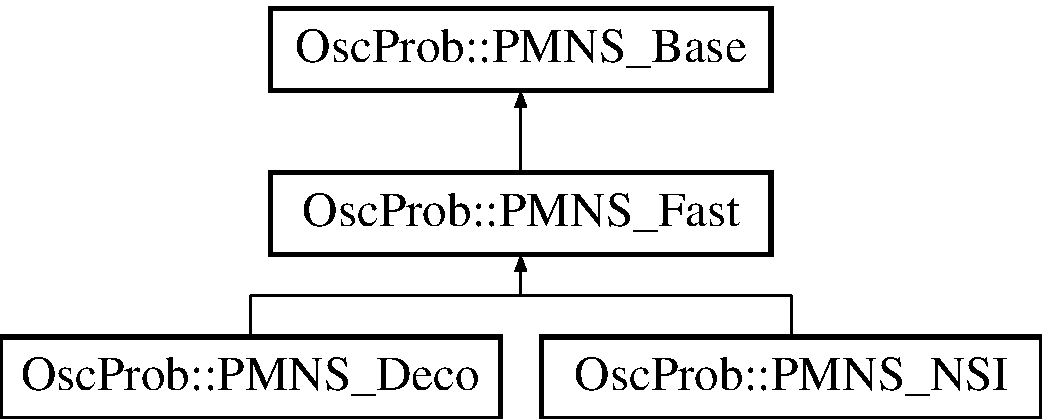
\includegraphics[height=3.000000cm]{classOscProb_1_1PMNS__Fast}
\end{center}
\end{figure}
\subsection*{Public Types}
\begin{DoxyCompactItemize}
\item 
typedef std\+::complex$<$ double $>$ \hyperlink{classOscProb_1_1PMNS__Base_ae86ec4718808ce9d02e5f5b4226714ab}{complex}
\end{DoxyCompactItemize}
\subsection*{Public Member Functions}
\begin{DoxyCompactItemize}
\item 
\hyperlink{classOscProb_1_1PMNS__Fast_a2bbac744bf63753105d766a860af7c0d}{P\+M\+N\+S\+\_\+\+Fast} ()
\begin{DoxyCompactList}\small\item\em Constructor. \end{DoxyCompactList}\item 
virtual \hyperlink{classOscProb_1_1PMNS__Fast_ae1b797dda260ff83793cdfe448f58878}{$\sim$\+P\+M\+N\+S\+\_\+\+Fast} ()
\begin{DoxyCompactList}\small\item\em Destructor. \end{DoxyCompactList}\item 
virtual void \hyperlink{classOscProb_1_1PMNS__Fast_ad849b2231d99c5d66fb3ade8efb896e1}{Set\+Mix} (double th12, double th23, double th13, double deltacp)
\begin{DoxyCompactList}\small\item\em Set the all mixing parameters at once. \end{DoxyCompactList}\item 
virtual void \hyperlink{classOscProb_1_1PMNS__Fast_a63733b246e6d2e609ce3de7a65ba5b9f}{Set\+Delta\+Msqrs} (double dm21, double dm32)
\begin{DoxyCompactList}\small\item\em Set both mass-\/splittings at once. \end{DoxyCompactList}\item 
virtual double \hyperlink{classOscProb_1_1PMNS__Base_aec5c399b93261f1962a4b7dbbb44b973}{Prob} (int flvi, int flvf)
\begin{DoxyCompactList}\small\item\em Compute the probability of flvi going to flvf. \end{DoxyCompactList}\item 
virtual double \hyperlink{classOscProb_1_1PMNS__Base_aa3cee10639d5c0879ccb9e78d62128d3}{Prob} (int flvi, int flvf, double E)
\begin{DoxyCompactList}\small\item\em Compute the probability of flvi going to flvf for energy E. \end{DoxyCompactList}\item 
virtual double \hyperlink{classOscProb_1_1PMNS__Base_a6e0a74508d9d6db7be02e242b8467563}{Prob} (int flvi, int flvf, double E, double L)
\begin{DoxyCompactList}\small\item\em Compute the probability of flvi going to flvf for energy E and distance L. \end{DoxyCompactList}\item 
virtual double \hyperlink{classOscProb_1_1PMNS__Base_ac03f754160422e6600da8dbae0f803ed}{Avg\+Prob} (int flvi, int flvf, double E, double dE=0)
\begin{DoxyCompactList}\small\item\em Compute the average probability over a bin of energy. \end{DoxyCompactList}\item 
virtual double \hyperlink{classOscProb_1_1PMNS__Base_ac19a92f4ef428a7333ca8eed76fca637}{Avg\+Prob\+LoE} (int flvi, int flvf, double LoE, double d\+LoE=0)
\begin{DoxyCompactList}\small\item\em Compute the average probability over a bin of L/E. \end{DoxyCompactList}\item 
virtual void \hyperlink{classOscProb_1_1PMNS__Base_ace7875cf6d3bec161a2b7ed2690aec34}{Set\+Angle} (int i, int j, double th)
\begin{DoxyCompactList}\small\item\em Set the mixing angle theta\+\_\+ij. \end{DoxyCompactList}\item 
virtual void \hyperlink{classOscProb_1_1PMNS__Base_a4bef78cfcfc4e70b4ce79cdb8862c0a3}{Set\+Delta} (int i, int j, double delta)
\begin{DoxyCompactList}\small\item\em Set the CP phase delta\+\_\+ij. \end{DoxyCompactList}\item 
virtual void \hyperlink{classOscProb_1_1PMNS__Base_a492243b22fb1b783cd2943f507cff970}{Set\+Dm} (int j, double dm)
\begin{DoxyCompactList}\small\item\em Set the mass-\/splitting dm\+\_\+j1 in e\+V$^\wedge$2. \end{DoxyCompactList}\item 
virtual double \hyperlink{classOscProb_1_1PMNS__Base_acee137091304c919642293ddf015bbc8}{Get\+Angle} (int i, int j)
\begin{DoxyCompactList}\small\item\em Get the mixing angle theta\+\_\+ij. \end{DoxyCompactList}\item 
virtual double \hyperlink{classOscProb_1_1PMNS__Base_adb8dbc91d4286d2e7c8f768c59476241}{Get\+Delta} (int i, int j)
\begin{DoxyCompactList}\small\item\em Get the CP phase delta\+\_\+ij. \end{DoxyCompactList}\item 
virtual double \hyperlink{classOscProb_1_1PMNS__Base_ad26815ac5f4805d1259817e4936e5f8f}{Get\+Dm} (int j)
\begin{DoxyCompactList}\small\item\em Get the mass-\/splitting dm\+\_\+j1 in e\+V$^\wedge$2. \end{DoxyCompactList}\item 
virtual void \hyperlink{classOscProb_1_1PMNS__Base_a4de96ac9b6d1e9b029ab877e57d211ad}{Set\+Std\+Pars} ()
\begin{DoxyCompactList}\small\item\em Set P\+DG 3-\/flavor parameters. \end{DoxyCompactList}\item 
virtual void \hyperlink{classOscProb_1_1PMNS__Base_a95b3b0d0cab5e6a54b5ef99587f837c0}{Set\+Energy} (double E)
\begin{DoxyCompactList}\small\item\em Set the neutrino energy in GeV. \end{DoxyCompactList}\item 
virtual void \hyperlink{classOscProb_1_1PMNS__Base_a717e0348cf762f3961854e332a9b52e0}{Set\+Is\+Nu\+Bar} (bool is\+Nu\+Bar)
\begin{DoxyCompactList}\small\item\em Set the anti-\/neutrino flag. \end{DoxyCompactList}\item 
virtual double \hyperlink{classOscProb_1_1PMNS__Base_acc0d46cc4b8f911b40b807225003bbed}{Get\+Energy} ()
\begin{DoxyCompactList}\small\item\em Get the neutrino energy in GeV. \end{DoxyCompactList}\item 
virtual bool \hyperlink{classOscProb_1_1PMNS__Base_a2f7f2a028dfe7a90fff6b4f757972c2c}{Get\+Is\+Nu\+Bar} ()
\begin{DoxyCompactList}\small\item\em Get the anti-\/neutrino flag. \end{DoxyCompactList}\item 
virtual void \hyperlink{classOscProb_1_1PMNS__Base_ac3b644fd0a56347d304ceca4ae9d8875}{Set\+Path} (\hyperlink{structOscProb_1_1NuPath}{Osc\+Prob\+::\+Nu\+Path} p)
\begin{DoxyCompactList}\small\item\em Set a single path. \end{DoxyCompactList}\item 
virtual void \hyperlink{classOscProb_1_1PMNS__Base_a35b983270613072a3df58b574d80dbfd}{Set\+Path} (double length, double density, double zoa=0.\+5, int layer=0)
\begin{DoxyCompactList}\small\item\em Set a single path. \end{DoxyCompactList}\item 
virtual void \hyperlink{classOscProb_1_1PMNS__Base_a637d19dd850b4246507796526622643c}{Set\+Path} (std\+::vector$<$ \hyperlink{structOscProb_1_1NuPath}{Osc\+Prob\+::\+Nu\+Path} $>$ paths)
\begin{DoxyCompactList}\small\item\em Set a path sequence. \end{DoxyCompactList}\item 
virtual void \hyperlink{classOscProb_1_1PMNS__Base_a887dc9d4dc569ec0cdef3933b4c60efc}{Add\+Path} (\hyperlink{structOscProb_1_1NuPath}{Osc\+Prob\+::\+Nu\+Path} p)
\begin{DoxyCompactList}\small\item\em Add a path to the sequence. \end{DoxyCompactList}\item 
virtual void \hyperlink{classOscProb_1_1PMNS__Base_ab7f89ad9e7e1224adaa59d3c41594cd9}{Add\+Path} (double length, double density, double zoa=0.\+5, int layer=0)
\begin{DoxyCompactList}\small\item\em Add a path to the sequence. \end{DoxyCompactList}\item 
virtual void \hyperlink{classOscProb_1_1PMNS__Base_aefe521239031c418cfaaaa550a6e13bb}{Clear\+Path} ()
\begin{DoxyCompactList}\small\item\em Clear the path vector. \end{DoxyCompactList}\item 
virtual void \hyperlink{classOscProb_1_1PMNS__Base_a6241325b1bd28cafa556daaecbe4ed62}{Set\+Length} (double L)
\begin{DoxyCompactList}\small\item\em Set a single path lentgh in km. \end{DoxyCompactList}\item 
virtual void \hyperlink{classOscProb_1_1PMNS__Base_aa34a40a3b5abda0f252982d9ead3b520}{Set\+Length} (std\+::vector$<$ double $>$ L)
\begin{DoxyCompactList}\small\item\em Set multiple path lengths. \end{DoxyCompactList}\item 
virtual void \hyperlink{classOscProb_1_1PMNS__Base_ac74206f349687da141392c81e2ba6b0d}{Set\+Density} (double rho)
\begin{DoxyCompactList}\small\item\em Set single path density in g/cm$^\wedge$3. \end{DoxyCompactList}\item 
virtual void \hyperlink{classOscProb_1_1PMNS__Base_a858221d5510fe732dc6a101fd305cda0}{Set\+Density} (std\+::vector$<$ double $>$ rho)
\begin{DoxyCompactList}\small\item\em Set multiple path densities. \end{DoxyCompactList}\item 
virtual void \hyperlink{classOscProb_1_1PMNS__Base_a1bf3ea8fd2507fd2fd82d7410ff8f578}{Set\+ZoA} (double zoa)
\begin{DoxyCompactList}\small\item\em Set Z/A value for single path. \end{DoxyCompactList}\item 
virtual void \hyperlink{classOscProb_1_1PMNS__Base_a8495f8a320e1a21965e6a64aec92ad2a}{Set\+ZoA} (std\+::vector$<$ double $>$ zoa)
\begin{DoxyCompactList}\small\item\em Set multiple path Z/A values. \end{DoxyCompactList}\item 
virtual void \hyperlink{classOscProb_1_1PMNS__Base_a904e580edf89fb98bf9a6397739b4ebe}{Set\+Layers} (std\+::vector$<$ int $>$ lay)
\begin{DoxyCompactList}\small\item\em Set multiple path layer indices. \end{DoxyCompactList}\item 
virtual void \hyperlink{classOscProb_1_1PMNS__Base_add6533a9fc9acdfc7ae258b62570d78d}{Set\+Std\+Path} ()
\begin{DoxyCompactList}\small\item\em Set standard neutrino path. \end{DoxyCompactList}\item 
virtual std\+::vector$<$ \hyperlink{structOscProb_1_1NuPath}{Osc\+Prob\+::\+Nu\+Path} $>$ \hyperlink{classOscProb_1_1PMNS__Base_ac8e196f2e85a2b1caaf705073ee95a5c}{Get\+Path} ()
\begin{DoxyCompactList}\small\item\em Get the neutrino path sequence. \end{DoxyCompactList}\item 
virtual std\+::vector$<$ double $>$ \hyperlink{classOscProb_1_1PMNS__Base_a9eac8d768c1424755ee41f7e783af179}{Get\+Sample\+Points} (double LoE, double d\+LoE)
\begin{DoxyCompactList}\small\item\em Compute the sample points for a bin of L/E with width d\+LoE. \end{DoxyCompactList}\end{DoxyCompactItemize}
\subsection*{Protected Member Functions}
\begin{DoxyCompactItemize}
\item 
virtual void \hyperlink{classOscProb_1_1PMNS__Fast_a16248082308f9d2c332ebf1be0aa90c3}{Update\+Ham} ()
\begin{DoxyCompactList}\small\item\em Build the full Hamiltonian. \end{DoxyCompactList}\item 
virtual void \hyperlink{classOscProb_1_1PMNS__Fast_a8a0828401591e88c60e0051fbfe02d5e}{Solve\+Ham} ()
\begin{DoxyCompactList}\small\item\em Solve the full Hamiltonian for eigenvectors and eigenvalues. \end{DoxyCompactList}\item 
virtual void \hyperlink{classOscProb_1_1PMNS__Fast_a76dd5a761df8689c502b28ad0391f9e2}{Set\+Vacuum\+Eigensystem} ()
\begin{DoxyCompactList}\small\item\em Set the eigensystem to the analytic solution of the vacuum Hamiltonian. \end{DoxyCompactList}\item 
virtual void \hyperlink{classOscProb_1_1PMNS__Base_adf23b569112f9f9e0e592f01d79a5f3d}{Initialize\+Vectors} ()
\begin{DoxyCompactList}\small\item\em Initialize all member vectors with zeros. \end{DoxyCompactList}\item 
virtual void \hyperlink{classOscProb_1_1PMNS__Base_a986e6ebef09a7e2eb7fee16a4c2c834d}{Set\+Cur\+Path} (\hyperlink{structOscProb_1_1NuPath}{Osc\+Prob\+::\+Nu\+Path} p)
\begin{DoxyCompactList}\small\item\em Set the path currently in use by the class. \end{DoxyCompactList}\item 
virtual void \hyperlink{classOscProb_1_1PMNS__Base_aba565962a440d14bee7a2a96d2eca2c5}{Set\+Att} (double att, int idx)
\begin{DoxyCompactList}\small\item\em Set one of the path attributes. \end{DoxyCompactList}\item 
virtual void \hyperlink{classOscProb_1_1PMNS__Base_aa001479b5f5828c3d16ed087f96ecbcc}{Set\+Att} (std\+::vector$<$ double $>$ att, int idx)
\begin{DoxyCompactList}\small\item\em Set all values of a path attribute. \end{DoxyCompactList}\item 
virtual void \hyperlink{classOscProb_1_1PMNS__Base_aae18afd69074211335f49ec40e6011b9}{RotateH} (int i, int j)
\begin{DoxyCompactList}\small\item\em Rotate the Hamiltonian by theta\+\_\+ij and delta\+\_\+ij. \end{DoxyCompactList}\item 
virtual void \hyperlink{classOscProb_1_1PMNS__Base_ad0faf5eae755afb1baa1fcd5ffebad41}{Build\+Hms} ()
\begin{DoxyCompactList}\small\item\em Build the matrix of masses squared. \end{DoxyCompactList}\item 
virtual void \hyperlink{classOscProb_1_1PMNS__Base_ac0d4bf8ff1318ef96d3dafa62e0cec25}{Reset\+To\+Flavour} (int flv)
\begin{DoxyCompactList}\small\item\em Reset neutrino state to pure flavour flv. \end{DoxyCompactList}\item 
virtual void \hyperlink{classOscProb_1_1PMNS__Base_accb08503acc162188041d7a96a280462}{Propagate\+Path} (\hyperlink{structOscProb_1_1NuPath}{Osc\+Prob\+::\+Nu\+Path} p)
\begin{DoxyCompactList}\small\item\em Propagate neutrino through a single path. \end{DoxyCompactList}\item 
virtual void \hyperlink{classOscProb_1_1PMNS__Base_a054e3a8b05b9a958b6fa416e4a835e3e}{Propagate} ()
\begin{DoxyCompactList}\small\item\em Propagate neutrino through full path. \end{DoxyCompactList}\item 
virtual double \hyperlink{classOscProb_1_1PMNS__Base_a0dc4d45bc3d7e03b9abbf5b4e100cc22}{P} (int flv)
\begin{DoxyCompactList}\small\item\em Return the probability of final state in flavour flv. \end{DoxyCompactList}\end{DoxyCompactItemize}
\subsection*{Protected Attributes}
\begin{DoxyCompactItemize}
\item 
\hyperlink{classOscProb_1_1PMNS__Base_ae86ec4718808ce9d02e5f5b4226714ab}{complex} \hyperlink{classOscProb_1_1PMNS__Fast_aab37f2a7f59ab7026a8a21a561115dd0}{f\+Ham} \mbox{[}3\mbox{]}\mbox{[}3\mbox{]}
\begin{DoxyCompactList}\small\item\em The full hamiltonian. \end{DoxyCompactList}\item 
int \hyperlink{classOscProb_1_1PMNS__Base_a24bb74bed63569dfe88b18fa6a08060e}{f\+Num\+Nus}
\begin{DoxyCompactList}\small\item\em Number of neutrino flavours. \end{DoxyCompactList}\item 
std\+::vector$<$ double $>$ \hyperlink{classOscProb_1_1PMNS__Base_a406a31c3b5d620e5a0cace5b411f9f70}{f\+Dm}
\begin{DoxyCompactList}\small\item\em m$^\wedge$2\+\_\+i -\/ m$^\wedge$2\+\_\+1 in vacuum \end{DoxyCompactList}\item 
std\+::vector$<$ std\+::vector$<$ double $>$ $>$ \hyperlink{classOscProb_1_1PMNS__Base_a1976887cd658dd86b2336c181f1470b4}{f\+Theta}
\begin{DoxyCompactList}\small\item\em theta\mbox{[}i\mbox{]}\mbox{[}j\mbox{]} mixing angle \end{DoxyCompactList}\item 
std\+::vector$<$ std\+::vector$<$ double $>$ $>$ \hyperlink{classOscProb_1_1PMNS__Base_ab2a5fa40e689b221c8a7d2c17213810d}{f\+Delta}
\begin{DoxyCompactList}\small\item\em delta\mbox{[}i\mbox{]}\mbox{[}j\mbox{]} CP violating phase \end{DoxyCompactList}\item 
std\+::vector$<$ \hyperlink{classOscProb_1_1PMNS__Base_ae86ec4718808ce9d02e5f5b4226714ab}{complex} $>$ \hyperlink{classOscProb_1_1PMNS__Base_ad38a7107c3ab393591fd5ba21658300b}{f\+Nu\+State}
\begin{DoxyCompactList}\small\item\em The neutrino current state. \end{DoxyCompactList}\item 
std\+::vector$<$ std\+::vector$<$ \hyperlink{classOscProb_1_1PMNS__Base_ae86ec4718808ce9d02e5f5b4226714ab}{complex} $>$ $>$ \hyperlink{classOscProb_1_1PMNS__Base_adf5901166216e8c7a5cff2092952f473}{f\+Hms}
\begin{DoxyCompactList}\small\item\em matrix H$\ast$2E in e\+V$^\wedge$2 \end{DoxyCompactList}\item 
std\+::vector$<$ double $>$ \hyperlink{classOscProb_1_1PMNS__Base_a6319c34d7decbb9d7d6da279c06e8c2d}{f\+Eval}
\begin{DoxyCompactList}\small\item\em Eigenvalues of the Hamiltonian. \end{DoxyCompactList}\item 
std\+::vector$<$ std\+::vector$<$ \hyperlink{classOscProb_1_1PMNS__Base_ae86ec4718808ce9d02e5f5b4226714ab}{complex} $>$ $>$ \hyperlink{classOscProb_1_1PMNS__Base_a093e7bd31d4ef52ed52df414e12c1d17}{f\+Evec}
\begin{DoxyCompactList}\small\item\em Eigenvectors of the Hamiltonian. \end{DoxyCompactList}\item 
double \hyperlink{classOscProb_1_1PMNS__Base_a2800af6d436972f3e900867790c046b0}{f\+Energy}
\begin{DoxyCompactList}\small\item\em Neutrino energy. \end{DoxyCompactList}\item 
bool \hyperlink{classOscProb_1_1PMNS__Base_a0ebaeaefab36a3ff381c6293faedfdd6}{f\+Is\+Nu\+Bar}
\begin{DoxyCompactList}\small\item\em Anti-\/neutrino flag. \end{DoxyCompactList}\item 
std\+::vector$<$ \hyperlink{structOscProb_1_1NuPath}{Osc\+Prob\+::\+Nu\+Path} $>$ \hyperlink{classOscProb_1_1PMNS__Base_a69db9d57e12fc7cbe0431bc6c18fac93}{f\+Nu\+Paths}
\begin{DoxyCompactList}\small\item\em Vector of neutrino paths. \end{DoxyCompactList}\item 
\hyperlink{structOscProb_1_1NuPath}{Osc\+Prob\+::\+Nu\+Path} \hyperlink{classOscProb_1_1PMNS__Base_a849437aa8891fe042e86886ce8f81c6e}{f\+Path}
\begin{DoxyCompactList}\small\item\em Current neutrino path. \end{DoxyCompactList}\item 
bool \hyperlink{classOscProb_1_1PMNS__Base_a9ac3cadeac8db1b90f3152f476244780}{f\+Built\+Hms}
\begin{DoxyCompactList}\small\item\em Tag to avoid rebuilding Hms. \end{DoxyCompactList}\item 
bool \hyperlink{classOscProb_1_1PMNS__Base_a6dc5cd010d2d70b2324745b4e53e9839}{f\+Got\+ES}
\begin{DoxyCompactList}\small\item\em Tag to avoid recalculating eigensystem. \end{DoxyCompactList}\end{DoxyCompactItemize}
\subsection*{Static Protected Attributes}
\begin{DoxyCompactItemize}
\item 
static const \hyperlink{classOscProb_1_1PMNS__Base_ae86ec4718808ce9d02e5f5b4226714ab}{complex} \hyperlink{classOscProb_1_1PMNS__Base_a5c31ed4593cf95feb36fb80c1850d25e}{zero}
\begin{DoxyCompactList}\small\item\em zero in complex \end{DoxyCompactList}\item 
static const \hyperlink{classOscProb_1_1PMNS__Base_ae86ec4718808ce9d02e5f5b4226714ab}{complex} \hyperlink{classOscProb_1_1PMNS__Base_ab64aab27448a5aca27565c991a9d173e}{one}
\begin{DoxyCompactList}\small\item\em one in complex \end{DoxyCompactList}\item 
static const double \hyperlink{classOscProb_1_1PMNS__Base_a382ddd7b76ca89b43f22614a2ea7327b}{k\+Km2eV} = 1.\+0 / 1.\+973269718e-\/10
\begin{DoxyCompactList}\small\item\em km to e\+V$^\wedge$-\/1 \end{DoxyCompactList}\item 
static const double \hyperlink{classOscProb_1_1PMNS__Base_a326fc5016d7dd7ce05682c06cdcb6d94}{k\+K2} = 4.\+62711501e-\/09
\begin{DoxyCompactList}\small\item\em mol/\+Ge\+V$^\wedge$2/cm$^\wedge$3 to eV \end{DoxyCompactList}\item 
static const double \hyperlink{classOscProb_1_1PMNS__Base_ad36a0a6bf58d6ec093d3947784bd89e9}{k\+Ge\+V2eV} = 1.\+0e+09
\begin{DoxyCompactList}\small\item\em GeV to eV. \end{DoxyCompactList}\item 
static const double \hyperlink{classOscProb_1_1PMNS__Base_a7f26a3456128234b2ae6cc9141a6532f}{k\+Gf} = 1.\+1663787e-\/05
\begin{DoxyCompactList}\small\item\em G\+\_\+F in units of Ge\+V$^\wedge$-\/2. \end{DoxyCompactList}\end{DoxyCompactItemize}


\subsection{Detailed Description}
Two optimizations are relevant\+:~\newline

\begin{DoxyItemize}
\item The construction of the Hamiltonian avoids computing null terms~\newline

\item The eigensystem determination is based on the following reference\+:~\newline
 
\begin{DoxyPre}
......................................................................\end{DoxyPre}

\end{DoxyItemize}


\begin{DoxyPre} Int. J. Mod. Phys. C       VOLUME 19, NUMBER 03            MARCH 2008\end{DoxyPre}



\begin{DoxyPre}     Efficient numerical diagonalization of hermitian 3x3 matrices\end{DoxyPre}



\begin{DoxyPre}                            Joachim Kopp
                  Max-Planck-Institut für Kernphysik 
             Postfach 10 39 80, 69029 Heidelberg, Germany
                    (Received 19 October 2007)\end{DoxyPre}



\begin{DoxyPre}                                523
......................................................................
 \end{DoxyPre}


\begin{DoxyAuthor}{Author}
Joao Coelho -\/ jcoelho@apc.\+in2p3.\+fr 
\end{DoxyAuthor}


Definition at line 36 of file P\+M\+N\+S\+\_\+\+Fast.\+h.



\subsection{Member Typedef Documentation}
\index{Osc\+Prob\+::\+P\+M\+N\+S\+\_\+\+Fast@{Osc\+Prob\+::\+P\+M\+N\+S\+\_\+\+Fast}!complex@{complex}}
\index{complex@{complex}!Osc\+Prob\+::\+P\+M\+N\+S\+\_\+\+Fast@{Osc\+Prob\+::\+P\+M\+N\+S\+\_\+\+Fast}}
\subsubsection[{\texorpdfstring{complex}{complex}}]{\setlength{\rightskip}{0pt plus 5cm}typedef std\+::complex$<$double$>$ {\bf Osc\+Prob\+::\+P\+M\+N\+S\+\_\+\+Base\+::complex}\hspace{0.3cm}{\ttfamily [inherited]}}\hypertarget{classOscProb_1_1PMNS__Base_ae86ec4718808ce9d02e5f5b4226714ab}{}\label{classOscProb_1_1PMNS__Base_ae86ec4718808ce9d02e5f5b4226714ab}


Definition at line 105 of file P\+M\+N\+S\+\_\+\+Base.\+h.



\subsection{Constructor \& Destructor Documentation}
\index{Osc\+Prob\+::\+P\+M\+N\+S\+\_\+\+Fast@{Osc\+Prob\+::\+P\+M\+N\+S\+\_\+\+Fast}!P\+M\+N\+S\+\_\+\+Fast@{P\+M\+N\+S\+\_\+\+Fast}}
\index{P\+M\+N\+S\+\_\+\+Fast@{P\+M\+N\+S\+\_\+\+Fast}!Osc\+Prob\+::\+P\+M\+N\+S\+\_\+\+Fast@{Osc\+Prob\+::\+P\+M\+N\+S\+\_\+\+Fast}}
\subsubsection[{\texorpdfstring{P\+M\+N\+S\+\_\+\+Fast()}{PMNS_Fast()}}]{\setlength{\rightskip}{0pt plus 5cm}P\+M\+N\+S\+\_\+\+Fast\+::\+P\+M\+N\+S\+\_\+\+Fast (
\begin{DoxyParamCaption}
{}
\end{DoxyParamCaption}
)}\hypertarget{classOscProb_1_1PMNS__Fast_a2bbac744bf63753105d766a860af7c0d}{}\label{classOscProb_1_1PMNS__Fast_a2bbac744bf63753105d766a860af7c0d}
Constructor. \begin{DoxySeeAlso}{See also}
\hyperlink{classOscProb_1_1PMNS__Base_aa53e83b03a9cf4bdfa0a07136bd17a79}{P\+M\+N\+S\+\_\+\+Base\+::\+P\+M\+N\+S\+\_\+\+Base}
\end{DoxySeeAlso}
This class is restricted to 3 neutrino flavours. 

Definition at line 24 of file P\+M\+N\+S\+\_\+\+Fast.\+cxx.


\begin{DoxyCode}
24 : \hyperlink{classOscProb_1_1PMNS__Base_aa53e83b03a9cf4bdfa0a07136bd17a79}{PMNS\_Base}(), \hyperlink{classOscProb_1_1PMNS__Fast_aab37f2a7f59ab7026a8a21a561115dd0}{fHam}() \{\}
\end{DoxyCode}
\index{Osc\+Prob\+::\+P\+M\+N\+S\+\_\+\+Fast@{Osc\+Prob\+::\+P\+M\+N\+S\+\_\+\+Fast}!````~P\+M\+N\+S\+\_\+\+Fast@{$\sim$\+P\+M\+N\+S\+\_\+\+Fast}}
\index{````~P\+M\+N\+S\+\_\+\+Fast@{$\sim$\+P\+M\+N\+S\+\_\+\+Fast}!Osc\+Prob\+::\+P\+M\+N\+S\+\_\+\+Fast@{Osc\+Prob\+::\+P\+M\+N\+S\+\_\+\+Fast}}
\subsubsection[{\texorpdfstring{$\sim$\+P\+M\+N\+S\+\_\+\+Fast()}{~PMNS_Fast()}}]{\setlength{\rightskip}{0pt plus 5cm}P\+M\+N\+S\+\_\+\+Fast\+::$\sim$\+P\+M\+N\+S\+\_\+\+Fast (
\begin{DoxyParamCaption}
{}
\end{DoxyParamCaption}
)\hspace{0.3cm}{\ttfamily [virtual]}}\hypertarget{classOscProb_1_1PMNS__Fast_ae1b797dda260ff83793cdfe448f58878}{}\label{classOscProb_1_1PMNS__Fast_ae1b797dda260ff83793cdfe448f58878}
Nothing to clean. 

Definition at line 30 of file P\+M\+N\+S\+\_\+\+Fast.\+cxx.


\begin{DoxyCode}
30 \{\}
\end{DoxyCode}


\subsection{Member Function Documentation}
\index{Osc\+Prob\+::\+P\+M\+N\+S\+\_\+\+Fast@{Osc\+Prob\+::\+P\+M\+N\+S\+\_\+\+Fast}!Add\+Path@{Add\+Path}}
\index{Add\+Path@{Add\+Path}!Osc\+Prob\+::\+P\+M\+N\+S\+\_\+\+Fast@{Osc\+Prob\+::\+P\+M\+N\+S\+\_\+\+Fast}}
\subsubsection[{\texorpdfstring{Add\+Path(\+Osc\+Prob\+::\+Nu\+Path p)}{AddPath(OscProb::NuPath p)}}]{\setlength{\rightskip}{0pt plus 5cm}void P\+M\+N\+S\+\_\+\+Base\+::\+Add\+Path (
\begin{DoxyParamCaption}
\item[{{\bf Osc\+Prob\+::\+Nu\+Path}}]{p}
\end{DoxyParamCaption}
)\hspace{0.3cm}{\ttfamily [virtual]}, {\ttfamily [inherited]}}\hypertarget{classOscProb_1_1PMNS__Base_a887dc9d4dc569ec0cdef3933b4c60efc}{}\label{classOscProb_1_1PMNS__Base_a887dc9d4dc569ec0cdef3933b4c60efc}
Add a path to the sequence. 
\begin{DoxyParams}{Parameters}
{\em p} & -\/ A neutrino path segment \\
\hline
\end{DoxyParams}


Definition at line 256 of file P\+M\+N\+S\+\_\+\+Base.\+cxx.



References Osc\+Prob\+::\+P\+M\+N\+S\+\_\+\+Base\+::f\+Nu\+Paths.



Referenced by Osc\+Prob\+::\+P\+M\+N\+S\+\_\+\+Base\+::\+Add\+Path(), Osc\+Prob\+::\+P\+M\+N\+S\+\_\+\+Base\+::\+Set\+Att(), and Osc\+Prob\+::\+P\+M\+N\+S\+\_\+\+Base\+::\+Set\+Path().


\begin{DoxyCode}
256                                \{
257 
258   \hyperlink{classOscProb_1_1PMNS__Base_a69db9d57e12fc7cbe0431bc6c18fac93}{fNuPaths}.push\_back(p);
259 
260 \}
\end{DoxyCode}
\index{Osc\+Prob\+::\+P\+M\+N\+S\+\_\+\+Fast@{Osc\+Prob\+::\+P\+M\+N\+S\+\_\+\+Fast}!Add\+Path@{Add\+Path}}
\index{Add\+Path@{Add\+Path}!Osc\+Prob\+::\+P\+M\+N\+S\+\_\+\+Fast@{Osc\+Prob\+::\+P\+M\+N\+S\+\_\+\+Fast}}
\subsubsection[{\texorpdfstring{Add\+Path(double length, double density, double zoa=0.\+5, int layer=0)}{AddPath(double length, double density, double zoa=0.5, int layer=0)}}]{\setlength{\rightskip}{0pt plus 5cm}void P\+M\+N\+S\+\_\+\+Base\+::\+Add\+Path (
\begin{DoxyParamCaption}
\item[{double}]{length, }
\item[{double}]{density, }
\item[{double}]{zoa = {\ttfamily 0.5}, }
\item[{int}]{layer = {\ttfamily 0}}
\end{DoxyParamCaption}
)\hspace{0.3cm}{\ttfamily [virtual]}, {\ttfamily [inherited]}}\hypertarget{classOscProb_1_1PMNS__Base_ab7f89ad9e7e1224adaa59d3c41594cd9}{}\label{classOscProb_1_1PMNS__Base_ab7f89ad9e7e1224adaa59d3c41594cd9}
Add a path to the sequence defining attributes directly. 
\begin{DoxyParams}{Parameters}
{\em length} & -\/ The length of the path segment in km \\
\hline
{\em density} & -\/ The density of the path segment in g/cm$^\wedge$3 \\
\hline
{\em zoa} & -\/ The effective Z/A of the path segment \\
\hline
{\em layer} & -\/ An index to identify the layer type (e.\+g. earth inner core) \\
\hline
\end{DoxyParams}


Definition at line 270 of file P\+M\+N\+S\+\_\+\+Base.\+cxx.



References Osc\+Prob\+::\+P\+M\+N\+S\+\_\+\+Base\+::\+Add\+Path().


\begin{DoxyCode}
270                                                                            \{
271 
272   \hyperlink{classOscProb_1_1PMNS__Base_a887dc9d4dc569ec0cdef3933b4c60efc}{AddPath}(\hyperlink{structOscProb_1_1NuPath}{NuPath}(length, density, zoa, layer));
273 
274 \}
\end{DoxyCode}
\index{Osc\+Prob\+::\+P\+M\+N\+S\+\_\+\+Fast@{Osc\+Prob\+::\+P\+M\+N\+S\+\_\+\+Fast}!Avg\+Prob@{Avg\+Prob}}
\index{Avg\+Prob@{Avg\+Prob}!Osc\+Prob\+::\+P\+M\+N\+S\+\_\+\+Fast@{Osc\+Prob\+::\+P\+M\+N\+S\+\_\+\+Fast}}
\subsubsection[{\texorpdfstring{Avg\+Prob(int flvi, int flvf, double E, double d\+E=0)}{AvgProb(int flvi, int flvf, double E, double dE=0)}}]{\setlength{\rightskip}{0pt plus 5cm}double P\+M\+N\+S\+\_\+\+Base\+::\+Avg\+Prob (
\begin{DoxyParamCaption}
\item[{int}]{flvi, }
\item[{int}]{flvf, }
\item[{double}]{E, }
\item[{double}]{dE = {\ttfamily 0}}
\end{DoxyParamCaption}
)\hspace{0.3cm}{\ttfamily [virtual]}, {\ttfamily [inherited]}}\hypertarget{classOscProb_1_1PMNS__Base_ac03f754160422e6600da8dbae0f803ed}{}\label{classOscProb_1_1PMNS__Base_ac03f754160422e6600da8dbae0f803ed}
Compute the average probability of flvi going to flvf over a bin of energy E with width dE.

This gets transformed into L/E, since the oscillation terms have arguments linear in L/E and not E.

This function currently only works for single paths.

Flavours are\+: 
\begin{DoxyPre}
  0 = nue, 1 = numu, 2 = nutau
  3 = sterile\_1, 4 = sterile\_2, etc.
\end{DoxyPre}
 
\begin{DoxyParams}{Parameters}
{\em flvi} & -\/ The neutrino starting flavour. \\
\hline
{\em flvf} & -\/ The neutrino final flavour. \\
\hline
{\em E} & -\/ The neutrino energy in the bin center in GeV \\
\hline
{\em dE} & -\/ The energy bin width in GeV\\
\hline
\end{DoxyParams}
\begin{DoxyReturn}{Returns}
Average neutrino oscillation probability 
\end{DoxyReturn}


Definition at line 1076 of file P\+M\+N\+S\+\_\+\+Base.\+cxx.



References Osc\+Prob\+::\+P\+M\+N\+S\+\_\+\+Base\+::\+Avg\+Prob\+Lo\+E(), Osc\+Prob\+::\+P\+M\+N\+S\+\_\+\+Base\+::f\+Nu\+Paths, Osc\+Prob\+::\+P\+M\+N\+S\+\_\+\+Base\+::f\+Path, Osc\+Prob\+::\+Nu\+Path\+::length, Osc\+Prob\+::\+P\+M\+N\+S\+\_\+\+Base\+::\+Prob(), and Osc\+Prob\+::\+P\+M\+N\+S\+\_\+\+Base\+::\+Set\+Cur\+Path().


\begin{DoxyCode}
1077 \{
1078 
1079   \textcolor{comment}{// Do nothing if energy is not positive}
1080   \textcolor{keywordflow}{if}(E<=0) \textcolor{keywordflow}{return} 0;
1081 
1082   \textcolor{keywordflow}{if}(\hyperlink{classOscProb_1_1PMNS__Base_a69db9d57e12fc7cbe0431bc6c18fac93}{fNuPaths}.empty()) \textcolor{keywordflow}{return} 0;
1083 
1084   \textcolor{keywordflow}{if}(\hyperlink{classOscProb_1_1PMNS__Base_a69db9d57e12fc7cbe0431bc6c18fac93}{fNuPaths}.size() != 1)\{
1085     cout << \textcolor{stringliteral}{"ERROR: AvgProb not implemented for multiple paths."} << endl;
1086     cout << \textcolor{stringliteral}{"       Returning probability at bin center."} << endl;
1087     \textcolor{keywordflow}{return} \hyperlink{classOscProb_1_1PMNS__Base_aec5c399b93261f1962a4b7dbbb44b973}{Prob}(flvi, flvf, E);
1088   \}
1089 
1090   \textcolor{comment}{// Don't average zero width}
1091   \textcolor{keywordflow}{if}(dE<=0) \textcolor{keywordflow}{return} \hyperlink{classOscProb_1_1PMNS__Base_aec5c399b93261f1962a4b7dbbb44b973}{Prob}(flvi, flvf, E);
1092 
1093   \textcolor{comment}{// Make sure fPath is set}
1094   \hyperlink{classOscProb_1_1PMNS__Base_a986e6ebef09a7e2eb7fee16a4c2c834d}{SetCurPath}(\hyperlink{classOscProb_1_1PMNS__Base_a69db9d57e12fc7cbe0431bc6c18fac93}{fNuPaths}[0]);
1095 
1096   \textcolor{comment}{// Define L/E variables}
1097   \textcolor{keywordtype}{double} LoE = 0;
1098   \textcolor{keywordtype}{double} dLoE = 0;
1099 
1100   \textcolor{comment}{// Set a minimum energy}
1101   \textcolor{keywordtype}{double} minE = 0.1 * E;
1102 
1103   \textcolor{comment}{// Transform range to L/E}
1104   \textcolor{comment}{// Full range if low edge > minE}
1105   \textcolor{keywordflow}{if}(E-dE/2 > minE)\{
1106     LoE = 0.5 * (\hyperlink{classOscProb_1_1PMNS__Base_a849437aa8891fe042e86886ce8f81c6e}{fPath}.\hyperlink{structOscProb_1_1NuPath_af22660894b6e25cf835500381b155557}{length}/(E-dE/2) + \hyperlink{classOscProb_1_1PMNS__Base_a849437aa8891fe042e86886ce8f81c6e}{fPath}.\hyperlink{structOscProb_1_1NuPath_af22660894b6e25cf835500381b155557}{length}/(E+dE/2));
1107     dLoE = \hyperlink{classOscProb_1_1PMNS__Base_a849437aa8891fe042e86886ce8f81c6e}{fPath}.\hyperlink{structOscProb_1_1NuPath_af22660894b6e25cf835500381b155557}{length}/(E-dE/2) - \hyperlink{classOscProb_1_1PMNS__Base_a849437aa8891fe042e86886ce8f81c6e}{fPath}.\hyperlink{structOscProb_1_1NuPath_af22660894b6e25cf835500381b155557}{length}/(E+dE/2);
1108   \}
1109   \textcolor{comment}{// Else start at minE}
1110   \textcolor{keywordflow}{else}\{
1111     LoE = 0.5 * (\hyperlink{classOscProb_1_1PMNS__Base_a849437aa8891fe042e86886ce8f81c6e}{fPath}.\hyperlink{structOscProb_1_1NuPath_af22660894b6e25cf835500381b155557}{length}/minE + \hyperlink{classOscProb_1_1PMNS__Base_a849437aa8891fe042e86886ce8f81c6e}{fPath}.\hyperlink{structOscProb_1_1NuPath_af22660894b6e25cf835500381b155557}{length}/(E+dE/2));
1112     dLoE = \hyperlink{classOscProb_1_1PMNS__Base_a849437aa8891fe042e86886ce8f81c6e}{fPath}.\hyperlink{structOscProb_1_1NuPath_af22660894b6e25cf835500381b155557}{length}/minE - \hyperlink{classOscProb_1_1PMNS__Base_a849437aa8891fe042e86886ce8f81c6e}{fPath}.\hyperlink{structOscProb_1_1NuPath_af22660894b6e25cf835500381b155557}{length}/(E+dE/2);
1113   \}
1114 
1115   \textcolor{comment}{// Compute average in LoE}
1116   \textcolor{keywordflow}{return} \hyperlink{classOscProb_1_1PMNS__Base_ac19a92f4ef428a7333ca8eed76fca637}{AvgProbLoE}(flvi, flvf, LoE, dLoE);
1117 
1118 \}
\end{DoxyCode}
\index{Osc\+Prob\+::\+P\+M\+N\+S\+\_\+\+Fast@{Osc\+Prob\+::\+P\+M\+N\+S\+\_\+\+Fast}!Avg\+Prob\+LoE@{Avg\+Prob\+LoE}}
\index{Avg\+Prob\+LoE@{Avg\+Prob\+LoE}!Osc\+Prob\+::\+P\+M\+N\+S\+\_\+\+Fast@{Osc\+Prob\+::\+P\+M\+N\+S\+\_\+\+Fast}}
\subsubsection[{\texorpdfstring{Avg\+Prob\+Lo\+E(int flvi, int flvf, double Lo\+E, double d\+Lo\+E=0)}{AvgProbLoE(int flvi, int flvf, double LoE, double dLoE=0)}}]{\setlength{\rightskip}{0pt plus 5cm}double P\+M\+N\+S\+\_\+\+Base\+::\+Avg\+Prob\+LoE (
\begin{DoxyParamCaption}
\item[{int}]{flvi, }
\item[{int}]{flvf, }
\item[{double}]{LoE, }
\item[{double}]{d\+LoE = {\ttfamily 0}}
\end{DoxyParamCaption}
)\hspace{0.3cm}{\ttfamily [virtual]}, {\ttfamily [inherited]}}\hypertarget{classOscProb_1_1PMNS__Base_ac19a92f4ef428a7333ca8eed76fca637}{}\label{classOscProb_1_1PMNS__Base_ac19a92f4ef428a7333ca8eed76fca637}
Compute the average probability of flvi going to flvf over a bin of L/E with width d\+LoE.

The probabilities are weighted by (L/E)$^\wedge$-\/2 so that event density is flat in energy. This avoids giving too much weight to low energies. Better approximations would be achieved if we used an interpolated event density.

This function currently only works for single paths.

Flavours are\+: 
\begin{DoxyPre}
  0 = nue, 1 = numu, 2 = nutau
  3 = sterile\_1, 4 = sterile\_2, etc.
\end{DoxyPre}
 
\begin{DoxyParams}{Parameters}
{\em flvi} & -\/ The neutrino starting flavour. \\
\hline
{\em flvf} & -\/ The neutrino final flavour. \\
\hline
{\em LoE} & -\/ The neutrino L/E value in the bin center in km/\+GeV \\
\hline
{\em d\+LoE} & -\/ The L/E bin width in km/\+GeV\\
\hline
\end{DoxyParams}
\begin{DoxyReturn}{Returns}
Average neutrino oscillation probability 
\end{DoxyReturn}


Definition at line 1144 of file P\+M\+N\+S\+\_\+\+Base.\+cxx.



References Osc\+Prob\+::\+P\+M\+N\+S\+\_\+\+Base\+::f\+Nu\+Paths, Osc\+Prob\+::\+P\+M\+N\+S\+\_\+\+Base\+::f\+Path, Osc\+Prob\+::\+P\+M\+N\+S\+\_\+\+Base\+::\+Get\+Sample\+Points(), Osc\+Prob\+::\+Nu\+Path\+::length, Osc\+Prob\+::\+P\+M\+N\+S\+\_\+\+Base\+::\+Prob(), Osc\+Prob\+::\+P\+M\+N\+S\+\_\+\+Base\+::\+Set\+Cur\+Path(), and Osc\+Prob\+::\+P\+M\+N\+S\+\_\+\+Base\+::\+Set\+Energy().



Referenced by Osc\+Prob\+::\+P\+M\+N\+S\+\_\+\+Base\+::\+Avg\+Prob().


\begin{DoxyCode}
1145 \{
1146 
1147   \textcolor{comment}{// Do nothing if L/E is not positive}
1148   \textcolor{keywordflow}{if}(LoE<=0) \textcolor{keywordflow}{return} 0;
1149 
1150   \textcolor{keywordflow}{if}(\hyperlink{classOscProb_1_1PMNS__Base_a69db9d57e12fc7cbe0431bc6c18fac93}{fNuPaths}.empty()) \textcolor{keywordflow}{return} 0;
1151 
1152   \textcolor{keywordflow}{if}(\hyperlink{classOscProb_1_1PMNS__Base_a69db9d57e12fc7cbe0431bc6c18fac93}{fNuPaths}.size() > 1)\{
1153 
1154     cout << \textcolor{stringliteral}{"ERROR: AvgProb not implemented for multiple paths."} << endl;
1155     cout << \textcolor{stringliteral}{"       Returning probability at bin center."} << endl;
1156 
1157     \textcolor{keywordtype}{double} L = 0;
1158     \textcolor{keywordflow}{for}(\textcolor{keywordtype}{int} i=0; i<int(\hyperlink{classOscProb_1_1PMNS__Base_a69db9d57e12fc7cbe0431bc6c18fac93}{fNuPaths}.size()); i++)\{
1159       L += \hyperlink{classOscProb_1_1PMNS__Base_a69db9d57e12fc7cbe0431bc6c18fac93}{fNuPaths}[i].length;
1160     \}
1161 
1162     \textcolor{keywordflow}{return} \hyperlink{classOscProb_1_1PMNS__Base_aec5c399b93261f1962a4b7dbbb44b973}{Prob}(flvi, flvf, L/LoE);
1163 
1164   \}
1165 
1166   \textcolor{comment}{// Make sure fPath is set}
1167   \hyperlink{classOscProb_1_1PMNS__Base_a986e6ebef09a7e2eb7fee16a4c2c834d}{SetCurPath}(\hyperlink{classOscProb_1_1PMNS__Base_a69db9d57e12fc7cbe0431bc6c18fac93}{fNuPaths}[0]);
1168 
1169   \textcolor{comment}{// Set the energy at bin center}
1170   \hyperlink{classOscProb_1_1PMNS__Base_a95b3b0d0cab5e6a54b5ef99587f837c0}{SetEnergy}(\hyperlink{classOscProb_1_1PMNS__Base_a849437aa8891fe042e86886ce8f81c6e}{fPath}.\hyperlink{structOscProb_1_1NuPath_af22660894b6e25cf835500381b155557}{length}/LoE);
1171 
1172   \textcolor{comment}{// Don't average zero width}
1173   \textcolor{keywordflow}{if}(dLoE<=0) \textcolor{keywordflow}{return} \hyperlink{classOscProb_1_1PMNS__Base_aec5c399b93261f1962a4b7dbbb44b973}{Prob}(flvi, flvf);
1174 
1175   \textcolor{comment}{// Get sample points for this bin}
1176   vector<double> samples = \hyperlink{classOscProb_1_1PMNS__Base_a9eac8d768c1424755ee41f7e783af179}{GetSamplePoints}(LoE, dLoE);
1177 
1178   \textcolor{comment}{// Variables to fill sample}
1179   \textcolor{comment}{// probabilities and weights}
1180   \textcolor{keywordtype}{double} sumw = 0;
1181   \textcolor{keywordtype}{double} prob = 0;
1182 
1183   \textcolor{comment}{// Loop over all sample points}
1184   \textcolor{keywordflow}{for}(\textcolor{keywordtype}{int} j=0; j<int(samples.size()); j++)\{
1185 
1186     \textcolor{comment}{// Set (L/E)^-2 weights}
1187     \textcolor{keywordtype}{double} w = 1./pow(samples[j],2);
1188 
1189     \textcolor{comment}{// Add weighted probability}
1190     prob += w * \hyperlink{classOscProb_1_1PMNS__Base_aec5c399b93261f1962a4b7dbbb44b973}{Prob}(flvi, flvf, \hyperlink{classOscProb_1_1PMNS__Base_a849437aa8891fe042e86886ce8f81c6e}{fPath}.\hyperlink{structOscProb_1_1NuPath_af22660894b6e25cf835500381b155557}{length} / samples[j]);
1191 
1192     \textcolor{comment}{// Increment sum of weights}
1193     sumw += w;
1194 
1195   \}
1196 
1197   \textcolor{comment}{// Return weighted average of probabilities}
1198   \textcolor{keywordflow}{return} prob / sumw;
1199 
1200 \}
\end{DoxyCode}
\index{Osc\+Prob\+::\+P\+M\+N\+S\+\_\+\+Fast@{Osc\+Prob\+::\+P\+M\+N\+S\+\_\+\+Fast}!Build\+Hms@{Build\+Hms}}
\index{Build\+Hms@{Build\+Hms}!Osc\+Prob\+::\+P\+M\+N\+S\+\_\+\+Fast@{Osc\+Prob\+::\+P\+M\+N\+S\+\_\+\+Fast}}
\subsubsection[{\texorpdfstring{Build\+Hms()}{BuildHms()}}]{\setlength{\rightskip}{0pt plus 5cm}void P\+M\+N\+S\+\_\+\+Base\+::\+Build\+Hms (
\begin{DoxyParamCaption}
{}
\end{DoxyParamCaption}
)\hspace{0.3cm}{\ttfamily [protected]}, {\ttfamily [virtual]}, {\ttfamily [inherited]}}\hypertarget{classOscProb_1_1PMNS__Base_ad0faf5eae755afb1baa1fcd5ffebad41}{}\label{classOscProb_1_1PMNS__Base_ad0faf5eae755afb1baa1fcd5ffebad41}
Build Hms = H$\ast$2E, where H is the Hamiltonian in vacuum on flavour basis and E is the neutrino energy in eV. Hms is effectively the matrix of masses squared.

This is a hermitian matrix, so only the upper triangular part needs to be filled

The construction of the Hamiltonian avoids computing terms that are simply zero. This has a big impact in the computation time. 

Definition at line 851 of file P\+M\+N\+S\+\_\+\+Base.\+cxx.



References Osc\+Prob\+::\+P\+M\+N\+S\+\_\+\+Base\+::f\+Built\+Hms, Osc\+Prob\+::\+P\+M\+N\+S\+\_\+\+Base\+::f\+Dm, Osc\+Prob\+::\+P\+M\+N\+S\+\_\+\+Base\+::f\+Got\+ES, Osc\+Prob\+::\+P\+M\+N\+S\+\_\+\+Base\+::f\+Hms, Osc\+Prob\+::\+P\+M\+N\+S\+\_\+\+Base\+::f\+Num\+Nus, and Osc\+Prob\+::\+P\+M\+N\+S\+\_\+\+Base\+::\+Rotate\+H().



Referenced by Osc\+Prob\+::\+P\+M\+N\+S\+\_\+\+Sterile\+::\+Solve\+Ham(), and Solve\+Ham().


\begin{DoxyCode}
852 \{
853 
854   \textcolor{comment}{// Check if anything changed}
855   \textcolor{keywordflow}{if}(\hyperlink{classOscProb_1_1PMNS__Base_a9ac3cadeac8db1b90f3152f476244780}{fBuiltHms}) \textcolor{keywordflow}{return};
856 
857   \textcolor{comment}{// Tag to recompute eigensystem}
858   \hyperlink{classOscProb_1_1PMNS__Base_a6dc5cd010d2d70b2324745b4e53e9839}{fGotES} = \textcolor{keyword}{false};
859 
860   \textcolor{keywordflow}{for}(\textcolor{keywordtype}{int} j=0; j<\hyperlink{classOscProb_1_1PMNS__Base_a24bb74bed63569dfe88b18fa6a08060e}{fNumNus}; j++)\{
861     \textcolor{comment}{// Set mass splitting}
862     \hyperlink{classOscProb_1_1PMNS__Base_adf5901166216e8c7a5cff2092952f473}{fHms}[j][j] = \hyperlink{classOscProb_1_1PMNS__Base_a406a31c3b5d620e5a0cace5b411f9f70}{fDm}[j];
863     \textcolor{comment}{// Reset off-diagonal elements}
864     \textcolor{keywordflow}{for}(\textcolor{keywordtype}{int} i=0; i<j; i++)\{
865       \hyperlink{classOscProb_1_1PMNS__Base_adf5901166216e8c7a5cff2092952f473}{fHms}[i][j] = 0;
866     \}
867     \textcolor{comment}{// Rotate j neutrinos}
868     \textcolor{keywordflow}{for}(\textcolor{keywordtype}{int} i=0; i<j; i++)\{
869       \hyperlink{classOscProb_1_1PMNS__Base_aae18afd69074211335f49ec40e6011b9}{RotateH}(i,j);
870     \}
871   \}
872 
873   \textcolor{comment}{// Tag as built}
874   \hyperlink{classOscProb_1_1PMNS__Base_a9ac3cadeac8db1b90f3152f476244780}{fBuiltHms} = \textcolor{keyword}{true};
875 
876 \}
\end{DoxyCode}
\index{Osc\+Prob\+::\+P\+M\+N\+S\+\_\+\+Fast@{Osc\+Prob\+::\+P\+M\+N\+S\+\_\+\+Fast}!Clear\+Path@{Clear\+Path}}
\index{Clear\+Path@{Clear\+Path}!Osc\+Prob\+::\+P\+M\+N\+S\+\_\+\+Fast@{Osc\+Prob\+::\+P\+M\+N\+S\+\_\+\+Fast}}
\subsubsection[{\texorpdfstring{Clear\+Path()}{ClearPath()}}]{\setlength{\rightskip}{0pt plus 5cm}void P\+M\+N\+S\+\_\+\+Base\+::\+Clear\+Path (
\begin{DoxyParamCaption}
{}
\end{DoxyParamCaption}
)\hspace{0.3cm}{\ttfamily [virtual]}, {\ttfamily [inherited]}}\hypertarget{classOscProb_1_1PMNS__Base_aefe521239031c418cfaaaa550a6e13bb}{}\label{classOscProb_1_1PMNS__Base_aefe521239031c418cfaaaa550a6e13bb}
Clear the path vector. 

Definition at line 224 of file P\+M\+N\+S\+\_\+\+Base.\+cxx.



References Osc\+Prob\+::\+P\+M\+N\+S\+\_\+\+Base\+::f\+Nu\+Paths.



Referenced by Osc\+Prob\+::\+P\+M\+N\+S\+\_\+\+Base\+::\+Set\+Att(), and Osc\+Prob\+::\+P\+M\+N\+S\+\_\+\+Base\+::\+Set\+Path().


\begin{DoxyCode}
224                          \{
225 
226   \hyperlink{classOscProb_1_1PMNS__Base_a69db9d57e12fc7cbe0431bc6c18fac93}{fNuPaths}.clear();
227 
228 \}
\end{DoxyCode}
\index{Osc\+Prob\+::\+P\+M\+N\+S\+\_\+\+Fast@{Osc\+Prob\+::\+P\+M\+N\+S\+\_\+\+Fast}!Get\+Angle@{Get\+Angle}}
\index{Get\+Angle@{Get\+Angle}!Osc\+Prob\+::\+P\+M\+N\+S\+\_\+\+Fast@{Osc\+Prob\+::\+P\+M\+N\+S\+\_\+\+Fast}}
\subsubsection[{\texorpdfstring{Get\+Angle(int i, int j)}{GetAngle(int i, int j)}}]{\setlength{\rightskip}{0pt plus 5cm}double P\+M\+N\+S\+\_\+\+Base\+::\+Get\+Angle (
\begin{DoxyParamCaption}
\item[{int}]{i, }
\item[{int}]{j}
\end{DoxyParamCaption}
)\hspace{0.3cm}{\ttfamily [virtual]}, {\ttfamily [inherited]}}\hypertarget{classOscProb_1_1PMNS__Base_acee137091304c919642293ddf015bbc8}{}\label{classOscProb_1_1PMNS__Base_acee137091304c919642293ddf015bbc8}
Get the mixing angle theta\+\_\+ij in radians.

Requires that i$<$j. Will notify you if input is wrong. If i$>$j, will assume reverse order and swap i and j.


\begin{DoxyParams}{Parameters}
{\em i,j} & -\/ the indices of theta\+\_\+ij \\
\hline
\end{DoxyParams}


Definition at line 563 of file P\+M\+N\+S\+\_\+\+Base.\+cxx.



References Osc\+Prob\+::\+P\+M\+N\+S\+\_\+\+Base\+::f\+Num\+Nus, and Osc\+Prob\+::\+P\+M\+N\+S\+\_\+\+Base\+::f\+Theta.


\begin{DoxyCode}
564 \{
565 
566   \textcolor{keywordflow}{if}(i>j)\{
567     cout << \textcolor{stringliteral}{"Warning: First argument should be smaller than second argument"} << endl;
568     cout << \textcolor{stringliteral}{"         Setting reverse order (Theta"} << j << i << \textcolor{stringliteral}{"). "} << endl;
569     \textcolor{keywordtype}{int} temp = i;
570     i = j;
571     j = temp;
572   \}
573   \textcolor{keywordflow}{if}(i<1 || i>\hyperlink{classOscProb_1_1PMNS__Base_a24bb74bed63569dfe88b18fa6a08060e}{fNumNus}-1 || j<2 || j>\hyperlink{classOscProb_1_1PMNS__Base_a24bb74bed63569dfe88b18fa6a08060e}{fNumNus})\{
574     cout << \textcolor{stringliteral}{"ERROR: Theta"} << i << j << \textcolor{stringliteral}{" not valid for "} << \hyperlink{classOscProb_1_1PMNS__Base_a24bb74bed63569dfe88b18fa6a08060e}{fNumNus};
575     cout << \textcolor{stringliteral}{" neutrinos. Returning zero."} << endl;
576     \textcolor{keywordflow}{return} 0;
577   \}
578 
579   \textcolor{keywordflow}{return} \hyperlink{classOscProb_1_1PMNS__Base_a1976887cd658dd86b2336c181f1470b4}{fTheta}[i-1][j-1];
580 
581 \}
\end{DoxyCode}
\index{Osc\+Prob\+::\+P\+M\+N\+S\+\_\+\+Fast@{Osc\+Prob\+::\+P\+M\+N\+S\+\_\+\+Fast}!Get\+Delta@{Get\+Delta}}
\index{Get\+Delta@{Get\+Delta}!Osc\+Prob\+::\+P\+M\+N\+S\+\_\+\+Fast@{Osc\+Prob\+::\+P\+M\+N\+S\+\_\+\+Fast}}
\subsubsection[{\texorpdfstring{Get\+Delta(int i, int j)}{GetDelta(int i, int j)}}]{\setlength{\rightskip}{0pt plus 5cm}double P\+M\+N\+S\+\_\+\+Base\+::\+Get\+Delta (
\begin{DoxyParamCaption}
\item[{int}]{i, }
\item[{int}]{j}
\end{DoxyParamCaption}
)\hspace{0.3cm}{\ttfamily [virtual]}, {\ttfamily [inherited]}}\hypertarget{classOscProb_1_1PMNS__Base_adb8dbc91d4286d2e7c8f768c59476241}{}\label{classOscProb_1_1PMNS__Base_adb8dbc91d4286d2e7c8f768c59476241}
Get the CP phase delta\+\_\+ij in radians.

Requires that i+1$<$j. Will notify you if input is wrong. If i$>$j, will assume reverse order and swap i and j.


\begin{DoxyParams}{Parameters}
{\em i,j} & -\/ the indices of delta\+\_\+ij \\
\hline
\end{DoxyParams}


Definition at line 633 of file P\+M\+N\+S\+\_\+\+Base.\+cxx.



References Osc\+Prob\+::\+P\+M\+N\+S\+\_\+\+Base\+::f\+Delta, and Osc\+Prob\+::\+P\+M\+N\+S\+\_\+\+Base\+::f\+Num\+Nus.


\begin{DoxyCode}
634 \{
635 
636   \textcolor{keywordflow}{if}(i>j)\{
637     cout << \textcolor{stringliteral}{"Warning: First argument should be smaller than second argument"} << endl;
638     cout << \textcolor{stringliteral}{"         Setting reverse order (Delta"} << j << i << \textcolor{stringliteral}{"). "} << endl;
639     \textcolor{keywordtype}{int} temp = i;
640     i = j;
641     j = temp;
642   \}
643   \textcolor{keywordflow}{if}(i<1 || i>\hyperlink{classOscProb_1_1PMNS__Base_a24bb74bed63569dfe88b18fa6a08060e}{fNumNus}-1 || j<2 || j>\hyperlink{classOscProb_1_1PMNS__Base_a24bb74bed63569dfe88b18fa6a08060e}{fNumNus})\{
644     cout << \textcolor{stringliteral}{"ERROR: Delta"} << i << j << \textcolor{stringliteral}{" not valid for "} << \hyperlink{classOscProb_1_1PMNS__Base_a24bb74bed63569dfe88b18fa6a08060e}{fNumNus};
645     cout << \textcolor{stringliteral}{" neutrinos. Returning zero."} << endl;
646     \textcolor{keywordflow}{return} 0;
647   \}
648   \textcolor{keywordflow}{if}(i+1==j)\{
649     cout << \textcolor{stringliteral}{"Warning: Rotation "} << i << j << \textcolor{stringliteral}{" is real. Returning zero."} << endl;
650     \textcolor{keywordflow}{return} 0;
651   \}
652 
653   \textcolor{keywordflow}{return} \hyperlink{classOscProb_1_1PMNS__Base_ab2a5fa40e689b221c8a7d2c17213810d}{fDelta}[i-1][j-1];
654 
655 \}
\end{DoxyCode}
\index{Osc\+Prob\+::\+P\+M\+N\+S\+\_\+\+Fast@{Osc\+Prob\+::\+P\+M\+N\+S\+\_\+\+Fast}!Get\+Dm@{Get\+Dm}}
\index{Get\+Dm@{Get\+Dm}!Osc\+Prob\+::\+P\+M\+N\+S\+\_\+\+Fast@{Osc\+Prob\+::\+P\+M\+N\+S\+\_\+\+Fast}}
\subsubsection[{\texorpdfstring{Get\+Dm(int j)}{GetDm(int j)}}]{\setlength{\rightskip}{0pt plus 5cm}double P\+M\+N\+S\+\_\+\+Base\+::\+Get\+Dm (
\begin{DoxyParamCaption}
\item[{int}]{j}
\end{DoxyParamCaption}
)\hspace{0.3cm}{\ttfamily [virtual]}, {\ttfamily [inherited]}}\hypertarget{classOscProb_1_1PMNS__Base_ad26815ac5f4805d1259817e4936e5f8f}{}\label{classOscProb_1_1PMNS__Base_ad26815ac5f4805d1259817e4936e5f8f}
Get the mass-\/splitting dm\+\_\+j1 = (m\+\_\+j$^\wedge$2 -\/ m\+\_\+1$^\wedge$2) in e\+V$^\wedge$2

Requires that j$>$1. Will notify you if input is wrong.


\begin{DoxyParams}{Parameters}
{\em j} & -\/ the index of dm\+\_\+j1 \\
\hline
\end{DoxyParams}


Definition at line 693 of file P\+M\+N\+S\+\_\+\+Base.\+cxx.



References Osc\+Prob\+::\+P\+M\+N\+S\+\_\+\+Base\+::f\+Dm, and Osc\+Prob\+::\+P\+M\+N\+S\+\_\+\+Base\+::f\+Num\+Nus.


\begin{DoxyCode}
694 \{
695 
696   \textcolor{keywordflow}{if}(j<2 || j>\hyperlink{classOscProb_1_1PMNS__Base_a24bb74bed63569dfe88b18fa6a08060e}{fNumNus})\{
697     cout << \textcolor{stringliteral}{"ERROR: Dm"} << j << \textcolor{stringliteral}{"1 not valid for "} << \hyperlink{classOscProb_1_1PMNS__Base_a24bb74bed63569dfe88b18fa6a08060e}{fNumNus};
698     cout << \textcolor{stringliteral}{" neutrinos. Returning zero."} << endl;
699     \textcolor{keywordflow}{return} 0;
700   \}
701 
702   \textcolor{keywordflow}{return} \hyperlink{classOscProb_1_1PMNS__Base_a406a31c3b5d620e5a0cace5b411f9f70}{fDm}[j-1];
703 
704 \}
\end{DoxyCode}
\index{Osc\+Prob\+::\+P\+M\+N\+S\+\_\+\+Fast@{Osc\+Prob\+::\+P\+M\+N\+S\+\_\+\+Fast}!Get\+Energy@{Get\+Energy}}
\index{Get\+Energy@{Get\+Energy}!Osc\+Prob\+::\+P\+M\+N\+S\+\_\+\+Fast@{Osc\+Prob\+::\+P\+M\+N\+S\+\_\+\+Fast}}
\subsubsection[{\texorpdfstring{Get\+Energy()}{GetEnergy()}}]{\setlength{\rightskip}{0pt plus 5cm}double P\+M\+N\+S\+\_\+\+Base\+::\+Get\+Energy (
\begin{DoxyParamCaption}
{}
\end{DoxyParamCaption}
)\hspace{0.3cm}{\ttfamily [virtual]}, {\ttfamily [inherited]}}\hypertarget{classOscProb_1_1PMNS__Base_acc0d46cc4b8f911b40b807225003bbed}{}\label{classOscProb_1_1PMNS__Base_acc0d46cc4b8f911b40b807225003bbed}
Get the neutrino energy in GeV. 

Definition at line 182 of file P\+M\+N\+S\+\_\+\+Base.\+cxx.



References Osc\+Prob\+::\+P\+M\+N\+S\+\_\+\+Base\+::f\+Energy.


\begin{DoxyCode}
182                             \{
183 
184   \textcolor{keywordflow}{return} \hyperlink{classOscProb_1_1PMNS__Base_a2800af6d436972f3e900867790c046b0}{fEnergy};
185 
186 \}
\end{DoxyCode}
\index{Osc\+Prob\+::\+P\+M\+N\+S\+\_\+\+Fast@{Osc\+Prob\+::\+P\+M\+N\+S\+\_\+\+Fast}!Get\+Is\+Nu\+Bar@{Get\+Is\+Nu\+Bar}}
\index{Get\+Is\+Nu\+Bar@{Get\+Is\+Nu\+Bar}!Osc\+Prob\+::\+P\+M\+N\+S\+\_\+\+Fast@{Osc\+Prob\+::\+P\+M\+N\+S\+\_\+\+Fast}}
\subsubsection[{\texorpdfstring{Get\+Is\+Nu\+Bar()}{GetIsNuBar()}}]{\setlength{\rightskip}{0pt plus 5cm}bool P\+M\+N\+S\+\_\+\+Base\+::\+Get\+Is\+Nu\+Bar (
\begin{DoxyParamCaption}
{}
\end{DoxyParamCaption}
)\hspace{0.3cm}{\ttfamily [virtual]}, {\ttfamily [inherited]}}\hypertarget{classOscProb_1_1PMNS__Base_a2f7f2a028dfe7a90fff6b4f757972c2c}{}\label{classOscProb_1_1PMNS__Base_a2f7f2a028dfe7a90fff6b4f757972c2c}
Get the anti-\/neutrino flag. 

Definition at line 192 of file P\+M\+N\+S\+\_\+\+Base.\+cxx.



References Osc\+Prob\+::\+P\+M\+N\+S\+\_\+\+Base\+::f\+Is\+Nu\+Bar.


\begin{DoxyCode}
192                            \{
193 
194   \textcolor{keywordflow}{return} \hyperlink{classOscProb_1_1PMNS__Base_a0ebaeaefab36a3ff381c6293faedfdd6}{fIsNuBar};
195 
196 \}
\end{DoxyCode}
\index{Osc\+Prob\+::\+P\+M\+N\+S\+\_\+\+Fast@{Osc\+Prob\+::\+P\+M\+N\+S\+\_\+\+Fast}!Get\+Path@{Get\+Path}}
\index{Get\+Path@{Get\+Path}!Osc\+Prob\+::\+P\+M\+N\+S\+\_\+\+Fast@{Osc\+Prob\+::\+P\+M\+N\+S\+\_\+\+Fast}}
\subsubsection[{\texorpdfstring{Get\+Path()}{GetPath()}}]{\setlength{\rightskip}{0pt plus 5cm}vector$<$ {\bf Nu\+Path} $>$ P\+M\+N\+S\+\_\+\+Base\+::\+Get\+Path (
\begin{DoxyParamCaption}
{}
\end{DoxyParamCaption}
)\hspace{0.3cm}{\ttfamily [virtual]}, {\ttfamily [inherited]}}\hypertarget{classOscProb_1_1PMNS__Base_ac8e196f2e85a2b1caaf705073ee95a5c}{}\label{classOscProb_1_1PMNS__Base_ac8e196f2e85a2b1caaf705073ee95a5c}
Get the vector of neutrino paths. 

Definition at line 245 of file P\+M\+N\+S\+\_\+\+Base.\+cxx.



References Osc\+Prob\+::\+P\+M\+N\+S\+\_\+\+Base\+::f\+Nu\+Paths.


\begin{DoxyCode}
245                                  \{
246 
247   \textcolor{keywordflow}{return} \hyperlink{classOscProb_1_1PMNS__Base_a69db9d57e12fc7cbe0431bc6c18fac93}{fNuPaths};
248 
249 \}
\end{DoxyCode}
\index{Osc\+Prob\+::\+P\+M\+N\+S\+\_\+\+Fast@{Osc\+Prob\+::\+P\+M\+N\+S\+\_\+\+Fast}!Get\+Sample\+Points@{Get\+Sample\+Points}}
\index{Get\+Sample\+Points@{Get\+Sample\+Points}!Osc\+Prob\+::\+P\+M\+N\+S\+\_\+\+Fast@{Osc\+Prob\+::\+P\+M\+N\+S\+\_\+\+Fast}}
\subsubsection[{\texorpdfstring{Get\+Sample\+Points(double Lo\+E, double d\+Lo\+E)}{GetSamplePoints(double LoE, double dLoE)}}]{\setlength{\rightskip}{0pt plus 5cm}vector$<$ double $>$ P\+M\+N\+S\+\_\+\+Base\+::\+Get\+Sample\+Points (
\begin{DoxyParamCaption}
\item[{double}]{LoE, }
\item[{double}]{d\+LoE}
\end{DoxyParamCaption}
)\hspace{0.3cm}{\ttfamily [virtual]}, {\ttfamily [inherited]}}\hypertarget{classOscProb_1_1PMNS__Base_a9eac8d768c1424755ee41f7e783af179}{}\label{classOscProb_1_1PMNS__Base_a9eac8d768c1424755ee41f7e783af179}
Compute the sample points for a bin of L/E with width d\+LoE

This is used for averaging the probability over a bin of L/E. It should be a private function, but I\textquotesingle{}m keeping it public for now for debugging purposes. The number of sample points seems too high for most purposes. The number of subdivisions needs to be optimized.


\begin{DoxyParams}{Parameters}
{\em LoE} & -\/ The neutrino L/E value in the bin center in km/\+GeV \\
\hline
{\em d\+LoE} & -\/ The L/E bin width in km/\+GeV \\
\hline
\end{DoxyParams}


Definition at line 1215 of file P\+M\+N\+S\+\_\+\+Base.\+cxx.



References Osc\+Prob\+::\+P\+M\+N\+S\+\_\+\+Base\+::f\+Energy, Osc\+Prob\+::\+P\+M\+N\+S\+\_\+\+Base\+::f\+Eval, Osc\+Prob\+::\+P\+M\+N\+S\+\_\+\+Base\+::f\+Num\+Nus, Osc\+Prob\+::\+P\+M\+N\+S\+\_\+\+Base\+::k\+Ge\+V2eV, Osc\+Prob\+::\+P\+M\+N\+S\+\_\+\+Base\+::k\+Km2eV, and Osc\+Prob\+::\+P\+M\+N\+S\+\_\+\+Base\+::\+Solve\+Ham().



Referenced by Osc\+Prob\+::\+P\+M\+N\+S\+\_\+\+Base\+::\+Avg\+Prob\+Lo\+E().


\begin{DoxyCode}
1216 \{
1217 
1218   \textcolor{comment}{// Solve Hamiltonian to get eigenvalues}
1219   \hyperlink{classOscProb_1_1PMNS__Base_a91f065cb9e910e0095e41462b4420b01}{SolveHam}();
1220 
1221   \textcolor{comment}{// Define conversion factor [km/GeV -> 1/(4 eV^2)]}
1222   \textcolor{keyword}{const} \textcolor{keywordtype}{double} k1267 = \hyperlink{classOscProb_1_1PMNS__Base_a382ddd7b76ca89b43f22614a2ea7327b}{kKm2eV} / (4 * \hyperlink{classOscProb_1_1PMNS__Base_ad36a0a6bf58d6ec093d3947784bd89e9}{kGeV2eV});
1223 
1224   \textcolor{comment}{// Get list of all effective Dm^2}
1225   vector<double> effDm;
1226 
1227   \textcolor{keywordflow}{for}(\textcolor{keywordtype}{int} i=0; i<\hyperlink{classOscProb_1_1PMNS__Base_a24bb74bed63569dfe88b18fa6a08060e}{fNumNus}-1; i++)\{
1228     \textcolor{keywordflow}{for}(\textcolor{keywordtype}{int} j=i+1; j<\hyperlink{classOscProb_1_1PMNS__Base_a24bb74bed63569dfe88b18fa6a08060e}{fNumNus}; j++)\{
1229       effDm.push\_back( 2 * \hyperlink{classOscProb_1_1PMNS__Base_ad36a0a6bf58d6ec093d3947784bd89e9}{kGeV2eV} * \hyperlink{classOscProb_1_1PMNS__Base_a2800af6d436972f3e900867790c046b0}{fEnergy} * fabs(\hyperlink{classOscProb_1_1PMNS__Base_a6319c34d7decbb9d7d6da279c06e8c2d}{fEval}[j] - 
      \hyperlink{classOscProb_1_1PMNS__Base_a6319c34d7decbb9d7d6da279c06e8c2d}{fEval}[i]) );
1230     \}
1231   \}
1232 
1233   \textcolor{keywordtype}{int} numDm = effDm.size();
1234 
1235   \textcolor{comment}{// Set a number of sub-divisions to achieve "good" accuracy}
1236   \textcolor{comment}{// This needs to be studied better}
1237   \textcolor{keywordtype}{int} n\_div = ceil( 20 * pow(dLoE/LoE,0.8) );
1238   \textcolor{comment}{//int n\_div = 1;}
1239 
1240   \textcolor{comment}{// A vector to store sample points}
1241   vector<double> allSamples;
1242 
1243   \textcolor{comment}{// Loop over sub-divisions}
1244   \textcolor{keywordflow}{for}(\textcolor{keywordtype}{int} k=0; k<n\_div; k++)\{
1245 
1246     \textcolor{comment}{// Define sub-division center and width}
1247     \textcolor{keywordtype}{double} bctr = LoE - dLoE/2 + (k+0.5)*dLoE/n\_div;
1248     \textcolor{keywordtype}{double} bwdt = dLoE/n\_div;
1249 
1250     \textcolor{comment}{// Make a list of indices sorted by Dm^2 value}
1251     vector<int> Idx(numDm, 0);
1252     \textcolor{keywordflow}{for}(\textcolor{keywordtype}{int} i=0; i<numDm; i++) Idx[i] = i;
1253     sort(Idx.begin(), Idx.end(), \hyperlink{structOscProb_1_1IdxCompare}{IdxCompare}(effDm));
1254 
1255     \textcolor{comment}{// Make a vector of L/E sample values}
1256     \textcolor{comment}{// Initialized in the sub-division center}
1257     vector<double> samples;
1258     samples.push\_back(bctr);
1259 
1260     \textcolor{comment}{// Loop over all Dm^2 to average each frequency}
1261     \textcolor{comment}{// This will recursively sample points in smaller}
1262     \textcolor{comment}{// bins so that all relevant frequencies are used}
1263     \textcolor{keywordflow}{for}(\textcolor{keywordtype}{int} i=0; i<numDm; i++)\{
1264 
1265       \textcolor{comment}{// Copy the list of sample L/E values}
1266       vector<double> prev = samples;
1267 
1268       \textcolor{comment}{// Redefine bin width to lie within full sub-division}
1269       \textcolor{keywordtype}{double} Width = 2*min(prev[0] - (bctr - bwdt/2), (bctr + bwdt/2) - prev[0]);
1270 
1271       \textcolor{comment}{// Compute oscillation argument sorted from lowest  to highest}
1272       \textcolor{keyword}{const} \textcolor{keywordtype}{double} arg = k1267 * effDm[Idx[i]] * Width;
1273 
1274       \textcolor{comment}{// Skip small oscillation values.}
1275       \textcolor{comment}{// If it's the last one, lower the tolerance}
1276       \textcolor{keywordflow}{if}(i < numDm-1)\{
1277         \textcolor{keywordflow}{if}(arg<0.9) \textcolor{keywordflow}{continue};
1278       \}
1279       \textcolor{keywordflow}{else}\{
1280         \textcolor{keywordflow}{if}(arg<0.1) \textcolor{keywordflow}{continue};
1281       \}
1282 
1283       \textcolor{comment}{// Reset samples to redefine them}
1284       samples.clear();
1285 
1286       \textcolor{comment}{// Loop over previous samples}
1287       \textcolor{keywordflow}{for}(\textcolor{keywordtype}{int} j=0; j<int(prev.size()); j++)\{
1288 
1289         \textcolor{comment}{// Compute new sample points around old samples}
1290         \textcolor{comment}{// This is based on a oscillatory quadrature rule}
1291         \textcolor{keywordtype}{double} sample = (1/sqrt(3)) * (Width/2);
1292         \textcolor{keywordflow}{if}(arg!=0) sample = acos(sin(arg)/arg)/arg * (Width/2);
1293 
1294         \textcolor{comment}{// Add samples above and below center}
1295         samples.push\_back(prev[j]-sample);
1296         samples.push\_back(prev[j]+sample);
1297 
1298       \}
1299 
1300     \}\textcolor{comment}{// End of loop over Dm^2}
1301 
1302     \textcolor{comment}{// Add sub-division samples to the end of allSamples vector}
1303     allSamples.insert(allSamples.end(), samples.begin(), samples.end());
1304 
1305   \}\textcolor{comment}{// End of loop over sub-divisions}
1306 
1307   \textcolor{comment}{// Return all sample points}
1308   \textcolor{keywordflow}{return} allSamples;
1309 
1310 \}
\end{DoxyCode}
\index{Osc\+Prob\+::\+P\+M\+N\+S\+\_\+\+Fast@{Osc\+Prob\+::\+P\+M\+N\+S\+\_\+\+Fast}!Initialize\+Vectors@{Initialize\+Vectors}}
\index{Initialize\+Vectors@{Initialize\+Vectors}!Osc\+Prob\+::\+P\+M\+N\+S\+\_\+\+Fast@{Osc\+Prob\+::\+P\+M\+N\+S\+\_\+\+Fast}}
\subsubsection[{\texorpdfstring{Initialize\+Vectors()}{InitializeVectors()}}]{\setlength{\rightskip}{0pt plus 5cm}void P\+M\+N\+S\+\_\+\+Base\+::\+Initialize\+Vectors (
\begin{DoxyParamCaption}
{}
\end{DoxyParamCaption}
)\hspace{0.3cm}{\ttfamily [protected]}, {\ttfamily [virtual]}, {\ttfamily [inherited]}}\hypertarget{classOscProb_1_1PMNS__Base_adf23b569112f9f9e0e592f01d79a5f3d}{}\label{classOscProb_1_1PMNS__Base_adf23b569112f9f9e0e592f01d79a5f3d}
Set vector sizes and initialize elements to zero. 

Definition at line 75 of file P\+M\+N\+S\+\_\+\+Base.\+cxx.



References Osc\+Prob\+::\+P\+M\+N\+S\+\_\+\+Base\+::f\+Delta, Osc\+Prob\+::\+P\+M\+N\+S\+\_\+\+Base\+::f\+Dm, Osc\+Prob\+::\+P\+M\+N\+S\+\_\+\+Base\+::f\+Eval, Osc\+Prob\+::\+P\+M\+N\+S\+\_\+\+Base\+::f\+Evec, Osc\+Prob\+::\+P\+M\+N\+S\+\_\+\+Base\+::f\+Hms, Osc\+Prob\+::\+P\+M\+N\+S\+\_\+\+Base\+::f\+Num\+Nus, Osc\+Prob\+::\+P\+M\+N\+S\+\_\+\+Base\+::f\+Nu\+State, Osc\+Prob\+::\+P\+M\+N\+S\+\_\+\+Base\+::f\+Theta, and Osc\+Prob\+::\+P\+M\+N\+S\+\_\+\+Base\+::zero.



Referenced by Osc\+Prob\+::\+P\+M\+N\+S\+\_\+\+Base\+::\+P\+M\+N\+S\+\_\+\+Base().


\begin{DoxyCode}
76 \{
77 
78   \hyperlink{classOscProb_1_1PMNS__Base_a406a31c3b5d620e5a0cace5b411f9f70}{fDm}    = vector<double>(\hyperlink{classOscProb_1_1PMNS__Base_a24bb74bed63569dfe88b18fa6a08060e}{fNumNus}, 0);
79   \hyperlink{classOscProb_1_1PMNS__Base_a1976887cd658dd86b2336c181f1470b4}{fTheta} = vector< vector<double> >(\hyperlink{classOscProb_1_1PMNS__Base_a24bb74bed63569dfe88b18fa6a08060e}{fNumNus}, vector<double>(\hyperlink{classOscProb_1_1PMNS__Base_a24bb74bed63569dfe88b18fa6a08060e}{fNumNus},0));
80   \hyperlink{classOscProb_1_1PMNS__Base_ab2a5fa40e689b221c8a7d2c17213810d}{fDelta} = vector< vector<double> >(\hyperlink{classOscProb_1_1PMNS__Base_a24bb74bed63569dfe88b18fa6a08060e}{fNumNus}, vector<double>(\hyperlink{classOscProb_1_1PMNS__Base_a24bb74bed63569dfe88b18fa6a08060e}{fNumNus},0));
81 
82   \hyperlink{classOscProb_1_1PMNS__Base_ad38a7107c3ab393591fd5ba21658300b}{fNuState} = vector<complex>(\hyperlink{classOscProb_1_1PMNS__Base_a24bb74bed63569dfe88b18fa6a08060e}{fNumNus}, \hyperlink{classOscProb_1_1PMNS__Base_a5c31ed4593cf95feb36fb80c1850d25e}{zero});
83   \hyperlink{classOscProb_1_1PMNS__Base_adf5901166216e8c7a5cff2092952f473}{fHms}     = vector< vector<complex> >(\hyperlink{classOscProb_1_1PMNS__Base_a24bb74bed63569dfe88b18fa6a08060e}{fNumNus}, vector<complex>(
      \hyperlink{classOscProb_1_1PMNS__Base_a24bb74bed63569dfe88b18fa6a08060e}{fNumNus},\hyperlink{classOscProb_1_1PMNS__Base_a5c31ed4593cf95feb36fb80c1850d25e}{zero}));
84 
85   \hyperlink{classOscProb_1_1PMNS__Base_a6319c34d7decbb9d7d6da279c06e8c2d}{fEval} = vector<double>(\hyperlink{classOscProb_1_1PMNS__Base_a24bb74bed63569dfe88b18fa6a08060e}{fNumNus}, 0);
86   \hyperlink{classOscProb_1_1PMNS__Base_a093e7bd31d4ef52ed52df414e12c1d17}{fEvec} = vector< vector<complex> >(\hyperlink{classOscProb_1_1PMNS__Base_a24bb74bed63569dfe88b18fa6a08060e}{fNumNus}, vector<complex>(\hyperlink{classOscProb_1_1PMNS__Base_a24bb74bed63569dfe88b18fa6a08060e}{fNumNus},
      \hyperlink{classOscProb_1_1PMNS__Base_a5c31ed4593cf95feb36fb80c1850d25e}{zero}));
87 
88 \}
\end{DoxyCode}
\index{Osc\+Prob\+::\+P\+M\+N\+S\+\_\+\+Fast@{Osc\+Prob\+::\+P\+M\+N\+S\+\_\+\+Fast}!P@{P}}
\index{P@{P}!Osc\+Prob\+::\+P\+M\+N\+S\+\_\+\+Fast@{Osc\+Prob\+::\+P\+M\+N\+S\+\_\+\+Fast}}
\subsubsection[{\texorpdfstring{P(int flv)}{P(int flv)}}]{\setlength{\rightskip}{0pt plus 5cm}double P\+M\+N\+S\+\_\+\+Base\+::P (
\begin{DoxyParamCaption}
\item[{int}]{flv}
\end{DoxyParamCaption}
)\hspace{0.3cm}{\ttfamily [protected]}, {\ttfamily [virtual]}, {\ttfamily [inherited]}}\hypertarget{classOscProb_1_1PMNS__Base_a0dc4d45bc3d7e03b9abbf5b4e100cc22}{}\label{classOscProb_1_1PMNS__Base_a0dc4d45bc3d7e03b9abbf5b4e100cc22}
Compute oscillation probability of flavour flv from current state

Flavours are\+: 
\begin{DoxyPre}
  0 = nue, 1 = numu, 2 = nutau
  3 = sterile\_1, 4 = sterile\_2, etc.
\end{DoxyPre}
 
\begin{DoxyParams}{Parameters}
{\em flv} & -\/ The neutrino final flavour.\\
\hline
\end{DoxyParams}
\begin{DoxyReturn}{Returns}
Neutrino oscillation probability 
\end{DoxyReturn}


Reimplemented in \hyperlink{classOscProb_1_1PMNS__Deco_aa81f47ea36207b90a5feb9849060032d}{Osc\+Prob\+::\+P\+M\+N\+S\+\_\+\+Deco}.



Definition at line 960 of file P\+M\+N\+S\+\_\+\+Base.\+cxx.



References Osc\+Prob\+::\+P\+M\+N\+S\+\_\+\+Base\+::f\+Num\+Nus, and Osc\+Prob\+::\+P\+M\+N\+S\+\_\+\+Base\+::f\+Nu\+State.



Referenced by Osc\+Prob\+::\+P\+M\+N\+S\+\_\+\+Base\+::\+Prob().


\begin{DoxyCode}
961 \{
962   assert(flv>=0 && flv<\hyperlink{classOscProb_1_1PMNS__Base_a24bb74bed63569dfe88b18fa6a08060e}{fNumNus});
963   \textcolor{keywordflow}{return} norm(\hyperlink{classOscProb_1_1PMNS__Base_ad38a7107c3ab393591fd5ba21658300b}{fNuState}[flv]);
964 \}
\end{DoxyCode}
\index{Osc\+Prob\+::\+P\+M\+N\+S\+\_\+\+Fast@{Osc\+Prob\+::\+P\+M\+N\+S\+\_\+\+Fast}!Prob@{Prob}}
\index{Prob@{Prob}!Osc\+Prob\+::\+P\+M\+N\+S\+\_\+\+Fast@{Osc\+Prob\+::\+P\+M\+N\+S\+\_\+\+Fast}}
\subsubsection[{\texorpdfstring{Prob(int flvi, int flvf)}{Prob(int flvi, int flvf)}}]{\setlength{\rightskip}{0pt plus 5cm}double P\+M\+N\+S\+\_\+\+Base\+::\+Prob (
\begin{DoxyParamCaption}
\item[{int}]{flvi, }
\item[{int}]{flvf}
\end{DoxyParamCaption}
)\hspace{0.3cm}{\ttfamily [virtual]}, {\ttfamily [inherited]}}\hypertarget{classOscProb_1_1PMNS__Base_aec5c399b93261f1962a4b7dbbb44b973}{}\label{classOscProb_1_1PMNS__Base_aec5c399b93261f1962a4b7dbbb44b973}
Compute the probability of flvi going to flvf.

Flavours are\+: 
\begin{DoxyPre}
  0 = nue, 1 = numu, 2 = nutau
  3 = sterile\_1, 4 = sterile\_2, etc.
\end{DoxyPre}
 
\begin{DoxyParams}{Parameters}
{\em flvi} & -\/ The neutrino starting flavour. \\
\hline
{\em flvf} & -\/ The neutrino final flavour.\\
\hline
\end{DoxyParams}
\begin{DoxyReturn}{Returns}
Neutrino oscillation probability 
\end{DoxyReturn}


Definition at line 980 of file P\+M\+N\+S\+\_\+\+Base.\+cxx.



References Osc\+Prob\+::\+P\+M\+N\+S\+\_\+\+Base\+::f\+Num\+Nus, Osc\+Prob\+::\+P\+M\+N\+S\+\_\+\+Base\+::\+P(), Osc\+Prob\+::\+P\+M\+N\+S\+\_\+\+Base\+::\+Propagate(), and Osc\+Prob\+::\+P\+M\+N\+S\+\_\+\+Base\+::\+Reset\+To\+Flavour().



Referenced by Osc\+Prob\+::\+P\+M\+N\+S\+\_\+\+Base\+::\+Avg\+Prob(), Osc\+Prob\+::\+P\+M\+N\+S\+\_\+\+Base\+::\+Avg\+Prob\+Lo\+E(), and Osc\+Prob\+::\+P\+M\+N\+S\+\_\+\+Base\+::\+Prob().


\begin{DoxyCode}
981 \{
982 
983   \textcolor{keywordflow}{if}(flvi < 0 || flvi >= \hyperlink{classOscProb_1_1PMNS__Base_a24bb74bed63569dfe88b18fa6a08060e}{fNumNus})\{
984     cout << \textcolor{stringliteral}{"ERROR: Initial flavour not in range: 0 - "} << \hyperlink{classOscProb_1_1PMNS__Base_a24bb74bed63569dfe88b18fa6a08060e}{fNumNus}-1 << endl;
985   \}
986   \textcolor{keywordflow}{if}(flvf < 0 || flvf >= \hyperlink{classOscProb_1_1PMNS__Base_a24bb74bed63569dfe88b18fa6a08060e}{fNumNus})\{
987     cout << \textcolor{stringliteral}{"ERROR: Final flavour not in range: 0 - "} << \hyperlink{classOscProb_1_1PMNS__Base_a24bb74bed63569dfe88b18fa6a08060e}{fNumNus}-1 << endl;
988   \}
989 
990   \hyperlink{classOscProb_1_1PMNS__Base_ac0d4bf8ff1318ef96d3dafa62e0cec25}{ResetToFlavour}(flvi);
991 
992   \hyperlink{classOscProb_1_1PMNS__Base_a054e3a8b05b9a958b6fa416e4a835e3e}{Propagate}();
993 
994   \textcolor{keywordflow}{return} \hyperlink{classOscProb_1_1PMNS__Base_a0dc4d45bc3d7e03b9abbf5b4e100cc22}{P}(flvf);
995 
996 \}
\end{DoxyCode}
\index{Osc\+Prob\+::\+P\+M\+N\+S\+\_\+\+Fast@{Osc\+Prob\+::\+P\+M\+N\+S\+\_\+\+Fast}!Prob@{Prob}}
\index{Prob@{Prob}!Osc\+Prob\+::\+P\+M\+N\+S\+\_\+\+Fast@{Osc\+Prob\+::\+P\+M\+N\+S\+\_\+\+Fast}}
\subsubsection[{\texorpdfstring{Prob(int flvi, int flvf, double E)}{Prob(int flvi, int flvf, double E)}}]{\setlength{\rightskip}{0pt plus 5cm}double P\+M\+N\+S\+\_\+\+Base\+::\+Prob (
\begin{DoxyParamCaption}
\item[{int}]{flvi, }
\item[{int}]{flvf, }
\item[{double}]{E}
\end{DoxyParamCaption}
)\hspace{0.3cm}{\ttfamily [virtual]}, {\ttfamily [inherited]}}\hypertarget{classOscProb_1_1PMNS__Base_aa3cee10639d5c0879ccb9e78d62128d3}{}\label{classOscProb_1_1PMNS__Base_aa3cee10639d5c0879ccb9e78d62128d3}
Compute the probability of flvi going to flvf for a given energy in GeV.

Flavours are\+: 
\begin{DoxyPre}
  0 = nue, 1 = numu, 2 = nutau
  3 = sterile\_1, 4 = sterile\_2, etc.
\end{DoxyPre}
 
\begin{DoxyParams}{Parameters}
{\em flvi} & -\/ The neutrino starting flavour. \\
\hline
{\em flvf} & -\/ The neutrino final flavour. \\
\hline
{\em E} & -\/ The neutrino energy in GeV\\
\hline
\end{DoxyParams}
\begin{DoxyReturn}{Returns}
Neutrino oscillation probability 
\end{DoxyReturn}


Definition at line 1013 of file P\+M\+N\+S\+\_\+\+Base.\+cxx.



References Osc\+Prob\+::\+P\+M\+N\+S\+\_\+\+Base\+::\+Prob(), and Osc\+Prob\+::\+P\+M\+N\+S\+\_\+\+Base\+::\+Set\+Energy().


\begin{DoxyCode}
1014 \{
1015 
1016   \hyperlink{classOscProb_1_1PMNS__Base_a95b3b0d0cab5e6a54b5ef99587f837c0}{SetEnergy}(E);
1017 
1018   \textcolor{keywordflow}{return} \hyperlink{classOscProb_1_1PMNS__Base_aec5c399b93261f1962a4b7dbbb44b973}{Prob}(flvi, flvf);
1019 
1020 \}
\end{DoxyCode}
\index{Osc\+Prob\+::\+P\+M\+N\+S\+\_\+\+Fast@{Osc\+Prob\+::\+P\+M\+N\+S\+\_\+\+Fast}!Prob@{Prob}}
\index{Prob@{Prob}!Osc\+Prob\+::\+P\+M\+N\+S\+\_\+\+Fast@{Osc\+Prob\+::\+P\+M\+N\+S\+\_\+\+Fast}}
\subsubsection[{\texorpdfstring{Prob(int flvi, int flvf, double E, double L)}{Prob(int flvi, int flvf, double E, double L)}}]{\setlength{\rightskip}{0pt plus 5cm}double P\+M\+N\+S\+\_\+\+Base\+::\+Prob (
\begin{DoxyParamCaption}
\item[{int}]{flvi, }
\item[{int}]{flvf, }
\item[{double}]{E, }
\item[{double}]{L}
\end{DoxyParamCaption}
)\hspace{0.3cm}{\ttfamily [virtual]}, {\ttfamily [inherited]}}\hypertarget{classOscProb_1_1PMNS__Base_a6e0a74508d9d6db7be02e242b8467563}{}\label{classOscProb_1_1PMNS__Base_a6e0a74508d9d6db7be02e242b8467563}
Compute the probability of flvi going to flvf for a given energy in GeV and distance in km in a single path.

If the path sequence is not a single path, a new single path will be created and the previous sequence will be lost.

Don\textquotesingle{}t use this if you want to propagate over multiple path segments.

Flavours are\+: 
\begin{DoxyPre}
  0 = nue, 1 = numu, 2 = nutau
  3 = sterile\_1, 4 = sterile\_2, etc.
\end{DoxyPre}
 
\begin{DoxyParams}{Parameters}
{\em flvi} & -\/ The neutrino starting flavour. \\
\hline
{\em flvf} & -\/ The neutrino final flavour. \\
\hline
{\em E} & -\/ The neutrino energy in GeV \\
\hline
{\em L} & -\/ The neutrino path length in km\\
\hline
\end{DoxyParams}
\begin{DoxyReturn}{Returns}
Neutrino oscillation probability 
\end{DoxyReturn}


Definition at line 1044 of file P\+M\+N\+S\+\_\+\+Base.\+cxx.



References Osc\+Prob\+::\+P\+M\+N\+S\+\_\+\+Base\+::\+Prob(), Osc\+Prob\+::\+P\+M\+N\+S\+\_\+\+Base\+::\+Set\+Energy(), and Osc\+Prob\+::\+P\+M\+N\+S\+\_\+\+Base\+::\+Set\+Length().


\begin{DoxyCode}
1045 \{
1046 
1047   \hyperlink{classOscProb_1_1PMNS__Base_a95b3b0d0cab5e6a54b5ef99587f837c0}{SetEnergy}(E);
1048   \hyperlink{classOscProb_1_1PMNS__Base_a6241325b1bd28cafa556daaecbe4ed62}{SetLength}(L);
1049 
1050   \textcolor{keywordflow}{return} \hyperlink{classOscProb_1_1PMNS__Base_aec5c399b93261f1962a4b7dbbb44b973}{Prob}(flvi, flvf);
1051 
1052 \}
\end{DoxyCode}
\index{Osc\+Prob\+::\+P\+M\+N\+S\+\_\+\+Fast@{Osc\+Prob\+::\+P\+M\+N\+S\+\_\+\+Fast}!Propagate@{Propagate}}
\index{Propagate@{Propagate}!Osc\+Prob\+::\+P\+M\+N\+S\+\_\+\+Fast@{Osc\+Prob\+::\+P\+M\+N\+S\+\_\+\+Fast}}
\subsubsection[{\texorpdfstring{Propagate()}{Propagate()}}]{\setlength{\rightskip}{0pt plus 5cm}void P\+M\+N\+S\+\_\+\+Base\+::\+Propagate (
\begin{DoxyParamCaption}
{}
\end{DoxyParamCaption}
)\hspace{0.3cm}{\ttfamily [protected]}, {\ttfamily [virtual]}, {\ttfamily [inherited]}}\hypertarget{classOscProb_1_1PMNS__Base_a054e3a8b05b9a958b6fa416e4a835e3e}{}\label{classOscProb_1_1PMNS__Base_a054e3a8b05b9a958b6fa416e4a835e3e}
Propagate neutrino state through full path 

Definition at line 916 of file P\+M\+N\+S\+\_\+\+Base.\+cxx.



References Osc\+Prob\+::\+P\+M\+N\+S\+\_\+\+Base\+::f\+Nu\+Paths, and Osc\+Prob\+::\+P\+M\+N\+S\+\_\+\+Base\+::\+Propagate\+Path().



Referenced by Osc\+Prob\+::\+P\+M\+N\+S\+\_\+\+Base\+::\+Prob().


\begin{DoxyCode}
917 \{
918 
919   \textcolor{keywordflow}{for}(\textcolor{keywordtype}{int} i=0; i<int(\hyperlink{classOscProb_1_1PMNS__Base_a69db9d57e12fc7cbe0431bc6c18fac93}{fNuPaths}.size()); i++)\{
920 
921     \hyperlink{classOscProb_1_1PMNS__Base_accb08503acc162188041d7a96a280462}{PropagatePath}(\hyperlink{classOscProb_1_1PMNS__Base_a69db9d57e12fc7cbe0431bc6c18fac93}{fNuPaths}[i]);
922 
923   \}
924 
925 \}
\end{DoxyCode}
\index{Osc\+Prob\+::\+P\+M\+N\+S\+\_\+\+Fast@{Osc\+Prob\+::\+P\+M\+N\+S\+\_\+\+Fast}!Propagate\+Path@{Propagate\+Path}}
\index{Propagate\+Path@{Propagate\+Path}!Osc\+Prob\+::\+P\+M\+N\+S\+\_\+\+Fast@{Osc\+Prob\+::\+P\+M\+N\+S\+\_\+\+Fast}}
\subsubsection[{\texorpdfstring{Propagate\+Path(\+Osc\+Prob\+::\+Nu\+Path p)}{PropagatePath(OscProb::NuPath p)}}]{\setlength{\rightskip}{0pt plus 5cm}void P\+M\+N\+S\+\_\+\+Base\+::\+Propagate\+Path (
\begin{DoxyParamCaption}
\item[{{\bf Osc\+Prob\+::\+Nu\+Path}}]{p}
\end{DoxyParamCaption}
)\hspace{0.3cm}{\ttfamily [protected]}, {\ttfamily [virtual]}, {\ttfamily [inherited]}}\hypertarget{classOscProb_1_1PMNS__Base_accb08503acc162188041d7a96a280462}{}\label{classOscProb_1_1PMNS__Base_accb08503acc162188041d7a96a280462}
Propagate the current neutrino state through a given path 
\begin{DoxyParams}{Parameters}
{\em p} & -\/ A neutrino path segment \\
\hline
\end{DoxyParams}


Reimplemented in \hyperlink{classOscProb_1_1PMNS__Deco_aa75341a3608bb12d7792a14e67ef2d5e}{Osc\+Prob\+::\+P\+M\+N\+S\+\_\+\+Deco}.



Definition at line 883 of file P\+M\+N\+S\+\_\+\+Base.\+cxx.



References Osc\+Prob\+::\+P\+M\+N\+S\+\_\+\+Base\+::f\+Eval, Osc\+Prob\+::\+P\+M\+N\+S\+\_\+\+Base\+::f\+Evec, Osc\+Prob\+::\+P\+M\+N\+S\+\_\+\+Base\+::f\+Num\+Nus, Osc\+Prob\+::\+P\+M\+N\+S\+\_\+\+Base\+::f\+Nu\+State, Osc\+Prob\+::\+P\+M\+N\+S\+\_\+\+Base\+::k\+Km2eV, Osc\+Prob\+::\+Nu\+Path\+::length, Osc\+Prob\+::\+P\+M\+N\+S\+\_\+\+Base\+::\+Set\+Cur\+Path(), Osc\+Prob\+::\+P\+M\+N\+S\+\_\+\+Base\+::\+Solve\+Ham(), and Osc\+Prob\+::\+P\+M\+N\+S\+\_\+\+Base\+::zero.



Referenced by Osc\+Prob\+::\+P\+M\+N\+S\+\_\+\+Base\+::\+Propagate().


\begin{DoxyCode}
884 \{
885 
886   \textcolor{comment}{// Set the neutrino path}
887   \hyperlink{classOscProb_1_1PMNS__Base_a986e6ebef09a7e2eb7fee16a4c2c834d}{SetCurPath}(p);
888 
889   \textcolor{comment}{// Solve for eigensystem}
890   \hyperlink{classOscProb_1_1PMNS__Base_a91f065cb9e910e0095e41462b4420b01}{SolveHam}();
891 
892   \textcolor{comment}{// Store coefficients of propagation eigenstates}
893   vector<complex> nuComp(\hyperlink{classOscProb_1_1PMNS__Base_a24bb74bed63569dfe88b18fa6a08060e}{fNumNus}, \hyperlink{classOscProb_1_1PMNS__Base_a5c31ed4593cf95feb36fb80c1850d25e}{zero});
894   \textcolor{keywordflow}{for}(\textcolor{keywordtype}{int} i=0;i<\hyperlink{classOscProb_1_1PMNS__Base_a24bb74bed63569dfe88b18fa6a08060e}{fNumNus};i++)\{
895     nuComp[i] = 0;
896     \textcolor{keywordflow}{for}(\textcolor{keywordtype}{int} j=0;j<\hyperlink{classOscProb_1_1PMNS__Base_a24bb74bed63569dfe88b18fa6a08060e}{fNumNus};j++)\{
897       nuComp[i] += \hyperlink{classOscProb_1_1PMNS__Base_ad38a7107c3ab393591fd5ba21658300b}{fNuState}[j] * conj(\hyperlink{classOscProb_1_1PMNS__Base_a093e7bd31d4ef52ed52df414e12c1d17}{fEvec}[j][i]);
898     \}
899   \}
900 
901   \textcolor{comment}{// Propagate neutrino state}
902   \textcolor{keywordflow}{for}(\textcolor{keywordtype}{int} i=0;i<\hyperlink{classOscProb_1_1PMNS__Base_a24bb74bed63569dfe88b18fa6a08060e}{fNumNus};i++)\{
903     \hyperlink{classOscProb_1_1PMNS__Base_ad38a7107c3ab393591fd5ba21658300b}{fNuState}[i] = 0;
904     \textcolor{keywordflow}{for}(\textcolor{keywordtype}{int} j=0;j<\hyperlink{classOscProb_1_1PMNS__Base_a24bb74bed63569dfe88b18fa6a08060e}{fNumNus};j++)\{
905       \textcolor{keywordtype}{double} arg = \hyperlink{classOscProb_1_1PMNS__Base_a6319c34d7decbb9d7d6da279c06e8c2d}{fEval}[j] * \hyperlink{classOscProb_1_1PMNS__Base_a382ddd7b76ca89b43f22614a2ea7327b}{kKm2eV} * p.\hyperlink{structOscProb_1_1NuPath_af22660894b6e25cf835500381b155557}{length};
906       \hyperlink{classOscProb_1_1PMNS__Base_ad38a7107c3ab393591fd5ba21658300b}{fNuState}[i] +=  \hyperlink{classOscProb_1_1PMNS__Base_ae86ec4718808ce9d02e5f5b4226714ab}{complex}(cos(arg), -sin(arg)) * nuComp[j] * 
      \hyperlink{classOscProb_1_1PMNS__Base_a093e7bd31d4ef52ed52df414e12c1d17}{fEvec}[i][j];
907     \}
908   \}
909 
910 \}
\end{DoxyCode}
\index{Osc\+Prob\+::\+P\+M\+N\+S\+\_\+\+Fast@{Osc\+Prob\+::\+P\+M\+N\+S\+\_\+\+Fast}!Reset\+To\+Flavour@{Reset\+To\+Flavour}}
\index{Reset\+To\+Flavour@{Reset\+To\+Flavour}!Osc\+Prob\+::\+P\+M\+N\+S\+\_\+\+Fast@{Osc\+Prob\+::\+P\+M\+N\+S\+\_\+\+Fast}}
\subsubsection[{\texorpdfstring{Reset\+To\+Flavour(int flv)}{ResetToFlavour(int flv)}}]{\setlength{\rightskip}{0pt plus 5cm}void P\+M\+N\+S\+\_\+\+Base\+::\+Reset\+To\+Flavour (
\begin{DoxyParamCaption}
\item[{int}]{flv}
\end{DoxyParamCaption}
)\hspace{0.3cm}{\ttfamily [protected]}, {\ttfamily [virtual]}, {\ttfamily [inherited]}}\hypertarget{classOscProb_1_1PMNS__Base_ac0d4bf8ff1318ef96d3dafa62e0cec25}{}\label{classOscProb_1_1PMNS__Base_ac0d4bf8ff1318ef96d3dafa62e0cec25}
Reset the neutrino state back to a pure flavour where it starts

Flavours are\+: 
\begin{DoxyPre}
  0 = nue, 1 = numu, 2 = nutau
  3 = sterile\_1, 4 = sterile\_2, etc.
\end{DoxyPre}
 
\begin{DoxyParams}{Parameters}
{\em flv} & -\/ The neutrino starting flavour. \\
\hline
\end{DoxyParams}


Reimplemented in \hyperlink{classOscProb_1_1PMNS__Deco_a393940f176614e3ffebeea40cfe78a62}{Osc\+Prob\+::\+P\+M\+N\+S\+\_\+\+Deco}.



Definition at line 938 of file P\+M\+N\+S\+\_\+\+Base.\+cxx.



References Osc\+Prob\+::\+P\+M\+N\+S\+\_\+\+Base\+::f\+Num\+Nus, Osc\+Prob\+::\+P\+M\+N\+S\+\_\+\+Base\+::f\+Nu\+State, Osc\+Prob\+::\+P\+M\+N\+S\+\_\+\+Base\+::one, and Osc\+Prob\+::\+P\+M\+N\+S\+\_\+\+Base\+::zero.



Referenced by Osc\+Prob\+::\+P\+M\+N\+S\+\_\+\+Base\+::\+P\+M\+N\+S\+\_\+\+Base(), and Osc\+Prob\+::\+P\+M\+N\+S\+\_\+\+Base\+::\+Prob().


\begin{DoxyCode}
939 \{
940   assert(flv>=0 && flv<\hyperlink{classOscProb_1_1PMNS__Base_a24bb74bed63569dfe88b18fa6a08060e}{fNumNus});
941   \textcolor{keywordflow}{for} (\textcolor{keywordtype}{int} i=0; i<\hyperlink{classOscProb_1_1PMNS__Base_a24bb74bed63569dfe88b18fa6a08060e}{fNumNus}; ++i)\{
942     \textcolor{keywordflow}{if} (i==flv) \hyperlink{classOscProb_1_1PMNS__Base_ad38a7107c3ab393591fd5ba21658300b}{fNuState}[i] = \hyperlink{classOscProb_1_1PMNS__Base_ab64aab27448a5aca27565c991a9d173e}{one};
943     \textcolor{keywordflow}{else}        \hyperlink{classOscProb_1_1PMNS__Base_ad38a7107c3ab393591fd5ba21658300b}{fNuState}[i] = \hyperlink{classOscProb_1_1PMNS__Base_a5c31ed4593cf95feb36fb80c1850d25e}{zero};
944   \}
945 \}
\end{DoxyCode}
\index{Osc\+Prob\+::\+P\+M\+N\+S\+\_\+\+Fast@{Osc\+Prob\+::\+P\+M\+N\+S\+\_\+\+Fast}!RotateH@{RotateH}}
\index{RotateH@{RotateH}!Osc\+Prob\+::\+P\+M\+N\+S\+\_\+\+Fast@{Osc\+Prob\+::\+P\+M\+N\+S\+\_\+\+Fast}}
\subsubsection[{\texorpdfstring{Rotate\+H(int i, int j)}{RotateH(int i, int j)}}]{\setlength{\rightskip}{0pt plus 5cm}void P\+M\+N\+S\+\_\+\+Base\+::\+RotateH (
\begin{DoxyParamCaption}
\item[{int}]{i, }
\item[{int}]{j}
\end{DoxyParamCaption}
)\hspace{0.3cm}{\ttfamily [protected]}, {\ttfamily [virtual]}, {\ttfamily [inherited]}}\hypertarget{classOscProb_1_1PMNS__Base_aae18afd69074211335f49ec40e6011b9}{}\label{classOscProb_1_1PMNS__Base_aae18afd69074211335f49ec40e6011b9}
Rotate the Hamiltonian by the angle theta\+\_\+ij and phase delta\+\_\+ij.

The rotations assume all off-\/diagonal elements with i $>$ j are zero. This is correct if the order of rotations is chosen appropriately and it speeds up computation by skipping null terms


\begin{DoxyParams}{Parameters}
{\em i,j} & -\/ the indices of the rotation ij \\
\hline
\end{DoxyParams}


Definition at line 717 of file P\+M\+N\+S\+\_\+\+Base.\+cxx.



References Osc\+Prob\+::\+P\+M\+N\+S\+\_\+\+Base\+::f\+Delta, Osc\+Prob\+::\+P\+M\+N\+S\+\_\+\+Base\+::f\+Hms, and Osc\+Prob\+::\+P\+M\+N\+S\+\_\+\+Base\+::f\+Theta.



Referenced by Osc\+Prob\+::\+P\+M\+N\+S\+\_\+\+Base\+::\+Build\+Hms().


\begin{DoxyCode}
717                                   \{
718 
719   \textcolor{comment}{// Do nothing if angle is zero}
720   \textcolor{keywordflow}{if}(\hyperlink{classOscProb_1_1PMNS__Base_a1976887cd658dd86b2336c181f1470b4}{fTheta}[i][j]==0) \textcolor{keywordflow}{return};
721 
722   \textcolor{keywordtype}{double} fSinBuffer = sin(\hyperlink{classOscProb_1_1PMNS__Base_a1976887cd658dd86b2336c181f1470b4}{fTheta}[i][j]);
723   \textcolor{keywordtype}{double} fCosBuffer = cos(\hyperlink{classOscProb_1_1PMNS__Base_a1976887cd658dd86b2336c181f1470b4}{fTheta}[i][j]);
724 
725   \textcolor{keywordtype}{double}  fHmsBufferD;
726   \hyperlink{classOscProb_1_1PMNS__Base_ae86ec4718808ce9d02e5f5b4226714ab}{complex} fHmsBufferC;
727 
728   \textcolor{comment}{// With Delta}
729   \textcolor{keywordflow}{if}(i+1<j)\{
730     \hyperlink{classOscProb_1_1PMNS__Base_ae86ec4718808ce9d02e5f5b4226714ab}{complex} fExpBuffer = \hyperlink{classOscProb_1_1PMNS__Base_ae86ec4718808ce9d02e5f5b4226714ab}{complex}(cos(\hyperlink{classOscProb_1_1PMNS__Base_ab2a5fa40e689b221c8a7d2c17213810d}{fDelta}[i][j]), -sin(
      \hyperlink{classOscProb_1_1PMNS__Base_ab2a5fa40e689b221c8a7d2c17213810d}{fDelta}[i][j]));
731 
732     \textcolor{comment}{// General case}
733     \textcolor{keywordflow}{if}(i>0)\{
734       \textcolor{comment}{// Top columns}
735       \textcolor{keywordflow}{for}(\textcolor{keywordtype}{int} k=0; k<i; k++)\{
736         fHmsBufferC = \hyperlink{classOscProb_1_1PMNS__Base_adf5901166216e8c7a5cff2092952f473}{fHms}[k][i];
737 
738         \hyperlink{classOscProb_1_1PMNS__Base_adf5901166216e8c7a5cff2092952f473}{fHms}[k][i] *= fCosBuffer;
739         \hyperlink{classOscProb_1_1PMNS__Base_adf5901166216e8c7a5cff2092952f473}{fHms}[k][i] += \hyperlink{classOscProb_1_1PMNS__Base_adf5901166216e8c7a5cff2092952f473}{fHms}[k][j] * fSinBuffer * conj(fExpBuffer);
740 
741         \hyperlink{classOscProb_1_1PMNS__Base_adf5901166216e8c7a5cff2092952f473}{fHms}[k][j] *= fCosBuffer;
742         \hyperlink{classOscProb_1_1PMNS__Base_adf5901166216e8c7a5cff2092952f473}{fHms}[k][j] -= fHmsBufferC * fSinBuffer * fExpBuffer;
743       \}
744 
745       \textcolor{comment}{// Middle row and column}
746       \textcolor{keywordflow}{for}(\textcolor{keywordtype}{int} k=i+1; k<j; k++)\{
747         fHmsBufferC = \hyperlink{classOscProb_1_1PMNS__Base_adf5901166216e8c7a5cff2092952f473}{fHms}[k][j];
748 
749         \hyperlink{classOscProb_1_1PMNS__Base_adf5901166216e8c7a5cff2092952f473}{fHms}[k][j] *= fCosBuffer;
750         \hyperlink{classOscProb_1_1PMNS__Base_adf5901166216e8c7a5cff2092952f473}{fHms}[k][j] -= conj(\hyperlink{classOscProb_1_1PMNS__Base_adf5901166216e8c7a5cff2092952f473}{fHms}[i][k]) * fSinBuffer * fExpBuffer;
751 
752         \hyperlink{classOscProb_1_1PMNS__Base_adf5901166216e8c7a5cff2092952f473}{fHms}[i][k] *= fCosBuffer;
753         \hyperlink{classOscProb_1_1PMNS__Base_adf5901166216e8c7a5cff2092952f473}{fHms}[i][k] += fSinBuffer * fExpBuffer * conj(fHmsBufferC);
754       \}
755 
756       \textcolor{comment}{// Nodes ij}
757       fHmsBufferC = \hyperlink{classOscProb_1_1PMNS__Base_adf5901166216e8c7a5cff2092952f473}{fHms}[i][i];
758       fHmsBufferD = real(\hyperlink{classOscProb_1_1PMNS__Base_adf5901166216e8c7a5cff2092952f473}{fHms}[j][j]);
759 
760       \hyperlink{classOscProb_1_1PMNS__Base_adf5901166216e8c7a5cff2092952f473}{fHms}[i][i] *= fCosBuffer * fCosBuffer;
761       \hyperlink{classOscProb_1_1PMNS__Base_adf5901166216e8c7a5cff2092952f473}{fHms}[i][i] += 2 * fSinBuffer * fCosBuffer * real(\hyperlink{classOscProb_1_1PMNS__Base_adf5901166216e8c7a5cff2092952f473}{fHms}[i][j] * conj(fExpBuffer));
762       \hyperlink{classOscProb_1_1PMNS__Base_adf5901166216e8c7a5cff2092952f473}{fHms}[i][i] += fSinBuffer * \hyperlink{classOscProb_1_1PMNS__Base_adf5901166216e8c7a5cff2092952f473}{fHms}[j][j] * fSinBuffer;
763 
764       \hyperlink{classOscProb_1_1PMNS__Base_adf5901166216e8c7a5cff2092952f473}{fHms}[j][j] *= fCosBuffer * fCosBuffer;
765       \hyperlink{classOscProb_1_1PMNS__Base_adf5901166216e8c7a5cff2092952f473}{fHms}[j][j] += fSinBuffer * fHmsBufferC * fSinBuffer;
766       \hyperlink{classOscProb_1_1PMNS__Base_adf5901166216e8c7a5cff2092952f473}{fHms}[j][j] -= 2 * fSinBuffer * fCosBuffer * real(\hyperlink{classOscProb_1_1PMNS__Base_adf5901166216e8c7a5cff2092952f473}{fHms}[i][j] * conj(fExpBuffer));
767 
768       \hyperlink{classOscProb_1_1PMNS__Base_adf5901166216e8c7a5cff2092952f473}{fHms}[i][j] -= 2 * fSinBuffer * real(\hyperlink{classOscProb_1_1PMNS__Base_adf5901166216e8c7a5cff2092952f473}{fHms}[i][j] * conj(fExpBuffer)) * fSinBuffer * fExpBuffer;
769       \hyperlink{classOscProb_1_1PMNS__Base_adf5901166216e8c7a5cff2092952f473}{fHms}[i][j] += fSinBuffer * fCosBuffer * (fHmsBufferD - fHmsBufferC) * fExpBuffer;
770 
771     \}
772     \textcolor{comment}{// First rotation on j (No top columns)}
773     \textcolor{keywordflow}{else}\{
774       \textcolor{comment}{// Middle rows and columns}
775       \textcolor{keywordflow}{for}(\textcolor{keywordtype}{int} k=i+1; k<j; k++)\{
776         \hyperlink{classOscProb_1_1PMNS__Base_adf5901166216e8c7a5cff2092952f473}{fHms}[k][j] = -conj(\hyperlink{classOscProb_1_1PMNS__Base_adf5901166216e8c7a5cff2092952f473}{fHms}[i][k]) * fSinBuffer * fExpBuffer;
777 
778         \hyperlink{classOscProb_1_1PMNS__Base_adf5901166216e8c7a5cff2092952f473}{fHms}[i][k] *= fCosBuffer;
779       \}
780 
781       \textcolor{comment}{// Nodes ij}
782       fHmsBufferD = real(\hyperlink{classOscProb_1_1PMNS__Base_adf5901166216e8c7a5cff2092952f473}{fHms}[i][i]);
783 
784       \hyperlink{classOscProb_1_1PMNS__Base_adf5901166216e8c7a5cff2092952f473}{fHms}[i][j] = fSinBuffer * fCosBuffer * (\hyperlink{classOscProb_1_1PMNS__Base_adf5901166216e8c7a5cff2092952f473}{fHms}[j][j] - fHmsBufferD) * fExpBuffer;
785 
786       \hyperlink{classOscProb_1_1PMNS__Base_adf5901166216e8c7a5cff2092952f473}{fHms}[i][i] *= fCosBuffer * fCosBuffer;
787       fHms[i][i] += fSinBuffer * fHms[j][j] * fSinBuffer;
788 
789       fHms[j][j] *= fCosBuffer * fCosBuffer;
790       fHms[j][j] += fSinBuffer * fHmsBufferD * fSinBuffer;
791     \}
792 
793   \}
794   \textcolor{comment}{// Without Delta (No middle rows or columns: j = i+1)}
795   \textcolor{keywordflow}{else}\{
796     \textcolor{comment}{// General case}
797     \textcolor{keywordflow}{if}(i>0)\{
798       \textcolor{comment}{// Top columns}
799       \textcolor{keywordflow}{for}(\textcolor{keywordtype}{int} k=0; k<i; k++)\{
800         fHmsBufferC = \hyperlink{classOscProb_1_1PMNS__Base_adf5901166216e8c7a5cff2092952f473}{fHms}[k][i];
801 
802         \hyperlink{classOscProb_1_1PMNS__Base_adf5901166216e8c7a5cff2092952f473}{fHms}[k][i] *= fCosBuffer;
803         \hyperlink{classOscProb_1_1PMNS__Base_adf5901166216e8c7a5cff2092952f473}{fHms}[k][i] += \hyperlink{classOscProb_1_1PMNS__Base_adf5901166216e8c7a5cff2092952f473}{fHms}[k][j] * fSinBuffer;
804 
805         \hyperlink{classOscProb_1_1PMNS__Base_adf5901166216e8c7a5cff2092952f473}{fHms}[k][j] *= fCosBuffer;
806         \hyperlink{classOscProb_1_1PMNS__Base_adf5901166216e8c7a5cff2092952f473}{fHms}[k][j] -= fHmsBufferC * fSinBuffer;
807       \}
808 
809       \textcolor{comment}{// Nodes ij}
810       fHmsBufferC = \hyperlink{classOscProb_1_1PMNS__Base_adf5901166216e8c7a5cff2092952f473}{fHms}[i][i];
811       fHmsBufferD = real(\hyperlink{classOscProb_1_1PMNS__Base_adf5901166216e8c7a5cff2092952f473}{fHms}[j][j]);
812 
813       \hyperlink{classOscProb_1_1PMNS__Base_adf5901166216e8c7a5cff2092952f473}{fHms}[i][i] *= fCosBuffer * fCosBuffer;
814       \hyperlink{classOscProb_1_1PMNS__Base_adf5901166216e8c7a5cff2092952f473}{fHms}[i][i] += 2 * fSinBuffer * fCosBuffer * real(\hyperlink{classOscProb_1_1PMNS__Base_adf5901166216e8c7a5cff2092952f473}{fHms}[i][j]);
815       \hyperlink{classOscProb_1_1PMNS__Base_adf5901166216e8c7a5cff2092952f473}{fHms}[i][i] += fSinBuffer * \hyperlink{classOscProb_1_1PMNS__Base_adf5901166216e8c7a5cff2092952f473}{fHms}[j][j] * fSinBuffer;
816 
817       \hyperlink{classOscProb_1_1PMNS__Base_adf5901166216e8c7a5cff2092952f473}{fHms}[j][j] *= fCosBuffer * fCosBuffer;
818       \hyperlink{classOscProb_1_1PMNS__Base_adf5901166216e8c7a5cff2092952f473}{fHms}[j][j] += fSinBuffer * fHmsBufferC * fSinBuffer;
819       \hyperlink{classOscProb_1_1PMNS__Base_adf5901166216e8c7a5cff2092952f473}{fHms}[j][j] -= 2 * fSinBuffer * fCosBuffer * real(\hyperlink{classOscProb_1_1PMNS__Base_adf5901166216e8c7a5cff2092952f473}{fHms}[i][j]);
820 
821       \hyperlink{classOscProb_1_1PMNS__Base_adf5901166216e8c7a5cff2092952f473}{fHms}[i][j] -= 2 * fSinBuffer * real(\hyperlink{classOscProb_1_1PMNS__Base_adf5901166216e8c7a5cff2092952f473}{fHms}[i][j]) * fSinBuffer;
822       \hyperlink{classOscProb_1_1PMNS__Base_adf5901166216e8c7a5cff2092952f473}{fHms}[i][j] += fSinBuffer * fCosBuffer * (fHmsBufferD - fHmsBufferC);
823 
824     \}
825     \textcolor{comment}{// First rotation (theta12)}
826     \textcolor{keywordflow}{else}\{
827 
828       \hyperlink{classOscProb_1_1PMNS__Base_adf5901166216e8c7a5cff2092952f473}{fHms}[i][j] = fSinBuffer * fCosBuffer * \hyperlink{classOscProb_1_1PMNS__Base_adf5901166216e8c7a5cff2092952f473}{fHms}[j][j];
829 
830       fHms[i][i] = fSinBuffer * fHms[j][j] * fSinBuffer;
831 
832       fHms[j][j] *= fCosBuffer * fCosBuffer;
833 
834     \}
835   \}
836 
837 \}
\end{DoxyCode}
\index{Osc\+Prob\+::\+P\+M\+N\+S\+\_\+\+Fast@{Osc\+Prob\+::\+P\+M\+N\+S\+\_\+\+Fast}!Set\+Angle@{Set\+Angle}}
\index{Set\+Angle@{Set\+Angle}!Osc\+Prob\+::\+P\+M\+N\+S\+\_\+\+Fast@{Osc\+Prob\+::\+P\+M\+N\+S\+\_\+\+Fast}}
\subsubsection[{\texorpdfstring{Set\+Angle(int i, int j, double th)}{SetAngle(int i, int j, double th)}}]{\setlength{\rightskip}{0pt plus 5cm}void P\+M\+N\+S\+\_\+\+Base\+::\+Set\+Angle (
\begin{DoxyParamCaption}
\item[{int}]{i, }
\item[{int}]{j, }
\item[{double}]{th}
\end{DoxyParamCaption}
)\hspace{0.3cm}{\ttfamily [virtual]}, {\ttfamily [inherited]}}\hypertarget{classOscProb_1_1PMNS__Base_ace7875cf6d3bec161a2b7ed2690aec34}{}\label{classOscProb_1_1PMNS__Base_ace7875cf6d3bec161a2b7ed2690aec34}
Set the mixing angle theta\+\_\+ij in radians.

Requires that i$<$j. Will notify you if input is wrong. If i$>$j, will assume reverse order and swap i and j.

This will check if value is changing to keep track of whether the hamiltonian needs to be rebuilt.


\begin{DoxyParams}{Parameters}
{\em i,j} & -\/ the indices of theta\+\_\+ij \\
\hline
{\em th} & -\/ the value of theta\+\_\+ij \\
\hline
\end{DoxyParams}


Definition at line 531 of file P\+M\+N\+S\+\_\+\+Base.\+cxx.



References Osc\+Prob\+::\+P\+M\+N\+S\+\_\+\+Base\+::f\+Built\+Hms, Osc\+Prob\+::\+P\+M\+N\+S\+\_\+\+Base\+::f\+Num\+Nus, and Osc\+Prob\+::\+P\+M\+N\+S\+\_\+\+Base\+::f\+Theta.



Referenced by Set\+Mix(), and Osc\+Prob\+::\+P\+M\+N\+S\+\_\+\+Base\+::\+Set\+Std\+Pars().


\begin{DoxyCode}
532 \{
533 
534   \textcolor{keywordflow}{if}(i>j)\{
535     cout << \textcolor{stringliteral}{"Warning: First argument should be smaller than second argument"} << endl;
536     cout << \textcolor{stringliteral}{"         Setting reverse order (Theta"} << j << i << \textcolor{stringliteral}{"). "} << endl;
537     \textcolor{keywordtype}{int} temp = i;
538     i = j;
539     j = temp;
540   \}
541   \textcolor{keywordflow}{if}(i<1 || i>\hyperlink{classOscProb_1_1PMNS__Base_a24bb74bed63569dfe88b18fa6a08060e}{fNumNus}-1 || j<2 || j>\hyperlink{classOscProb_1_1PMNS__Base_a24bb74bed63569dfe88b18fa6a08060e}{fNumNus})\{
542     cout << \textcolor{stringliteral}{"ERROR: Theta"} << i << j << \textcolor{stringliteral}{" not valid for "} << \hyperlink{classOscProb_1_1PMNS__Base_a24bb74bed63569dfe88b18fa6a08060e}{fNumNus};
543     cout << \textcolor{stringliteral}{" neutrinos. Doing nothing."} << endl;
544     \textcolor{keywordflow}{return};
545   \}
546 
547   \textcolor{comment}{// Check if value is actually changing}
548   \hyperlink{classOscProb_1_1PMNS__Base_a9ac3cadeac8db1b90f3152f476244780}{fBuiltHms} *= (\hyperlink{classOscProb_1_1PMNS__Base_a1976887cd658dd86b2336c181f1470b4}{fTheta}[i-1][j-1] == th);
549 
550   \hyperlink{classOscProb_1_1PMNS__Base_a1976887cd658dd86b2336c181f1470b4}{fTheta}[i-1][j-1] = th;
551 
552 \}
\end{DoxyCode}
\index{Osc\+Prob\+::\+P\+M\+N\+S\+\_\+\+Fast@{Osc\+Prob\+::\+P\+M\+N\+S\+\_\+\+Fast}!Set\+Att@{Set\+Att}}
\index{Set\+Att@{Set\+Att}!Osc\+Prob\+::\+P\+M\+N\+S\+\_\+\+Fast@{Osc\+Prob\+::\+P\+M\+N\+S\+\_\+\+Fast}}
\subsubsection[{\texorpdfstring{Set\+Att(double att, int idx)}{SetAtt(double att, int idx)}}]{\setlength{\rightskip}{0pt plus 5cm}void P\+M\+N\+S\+\_\+\+Base\+::\+Set\+Att (
\begin{DoxyParamCaption}
\item[{double}]{att, }
\item[{int}]{idx}
\end{DoxyParamCaption}
)\hspace{0.3cm}{\ttfamily [protected]}, {\ttfamily [virtual]}, {\ttfamily [inherited]}}\hypertarget{classOscProb_1_1PMNS__Base_aba565962a440d14bee7a2a96d2eca2c5}{}\label{classOscProb_1_1PMNS__Base_aba565962a440d14bee7a2a96d2eca2c5}
Set some single path attribute.

An auxiliary function to set individual attributes in a single path.

If the path sequence is not a single path, a new single path will be created and the previous sequence will be lost. Use with care.


\begin{DoxyParams}{Parameters}
{\em att} & -\/ The value of the attribute \\
\hline
{\em idx} & -\/ The index of the attribute (0,1,2,3) = (L, Rho, Z/A, Layer) \\
\hline
\end{DoxyParams}


Definition at line 320 of file P\+M\+N\+S\+\_\+\+Base.\+cxx.



References Osc\+Prob\+::\+P\+M\+N\+S\+\_\+\+Base\+::f\+Nu\+Paths, and Osc\+Prob\+::\+P\+M\+N\+S\+\_\+\+Base\+::\+Set\+Std\+Path().



Referenced by Osc\+Prob\+::\+P\+M\+N\+S\+\_\+\+Base\+::\+Set\+Density(), Osc\+Prob\+::\+P\+M\+N\+S\+\_\+\+Base\+::\+Set\+Layers(), Osc\+Prob\+::\+P\+M\+N\+S\+\_\+\+Base\+::\+Set\+Length(), and Osc\+Prob\+::\+P\+M\+N\+S\+\_\+\+Base\+::\+Set\+Zo\+A().


\begin{DoxyCode}
320                                          \{
321 
322   \textcolor{keywordflow}{if}(\hyperlink{classOscProb_1_1PMNS__Base_a69db9d57e12fc7cbe0431bc6c18fac93}{fNuPaths}.size() != 1)\{
323 
324     cout << \textcolor{stringliteral}{"Warning: Clearing path vector and starting new single path."} << endl;
325     cout << \textcolor{stringliteral}{"To avoid possible issues, use the SetPath function."} << endl;
326 
327     \hyperlink{classOscProb_1_1PMNS__Base_add6533a9fc9acdfc7ae258b62570d78d}{SetStdPath}();
328 
329   \}
330 
331   \textcolor{keywordflow}{switch}(idx)\{
332     \textcolor{keywordflow}{case} 0: \hyperlink{classOscProb_1_1PMNS__Base_a69db9d57e12fc7cbe0431bc6c18fac93}{fNuPaths}[0].length  = att; \textcolor{keywordflow}{break};
333     \textcolor{keywordflow}{case} 1: \hyperlink{classOscProb_1_1PMNS__Base_a69db9d57e12fc7cbe0431bc6c18fac93}{fNuPaths}[0].density = att; \textcolor{keywordflow}{break};
334     \textcolor{keywordflow}{case} 2: \hyperlink{classOscProb_1_1PMNS__Base_a69db9d57e12fc7cbe0431bc6c18fac93}{fNuPaths}[0].zoa     = att; \textcolor{keywordflow}{break};
335     \textcolor{keywordflow}{case} 3: \hyperlink{classOscProb_1_1PMNS__Base_a69db9d57e12fc7cbe0431bc6c18fac93}{fNuPaths}[0].layer   = att; \textcolor{keywordflow}{break};
336   \}
337 
338 \}
\end{DoxyCode}
\index{Osc\+Prob\+::\+P\+M\+N\+S\+\_\+\+Fast@{Osc\+Prob\+::\+P\+M\+N\+S\+\_\+\+Fast}!Set\+Att@{Set\+Att}}
\index{Set\+Att@{Set\+Att}!Osc\+Prob\+::\+P\+M\+N\+S\+\_\+\+Fast@{Osc\+Prob\+::\+P\+M\+N\+S\+\_\+\+Fast}}
\subsubsection[{\texorpdfstring{Set\+Att(std\+::vector$<$ double $>$ att, int idx)}{SetAtt(std::vector< double > att, int idx)}}]{\setlength{\rightskip}{0pt plus 5cm}void P\+M\+N\+S\+\_\+\+Base\+::\+Set\+Att (
\begin{DoxyParamCaption}
\item[{std\+::vector$<$ double $>$}]{att, }
\item[{int}]{idx}
\end{DoxyParamCaption}
)\hspace{0.3cm}{\ttfamily [protected]}, {\ttfamily [virtual]}, {\ttfamily [inherited]}}\hypertarget{classOscProb_1_1PMNS__Base_aa001479b5f5828c3d16ed087f96ecbcc}{}\label{classOscProb_1_1PMNS__Base_aa001479b5f5828c3d16ed087f96ecbcc}
Set all values of a path attribute.

An auxiliary function to set individual attributes in a path sequence.

If the path sequence is of a different size, a new path sequence will be created and the previous sequence will be lost. Use with care.


\begin{DoxyParams}{Parameters}
{\em att} & -\/ The values of the attribute \\
\hline
{\em idx} & -\/ The index of the attribute (0,1,2,3) = (L, Rho, Z/A, Layer) \\
\hline
\end{DoxyParams}


Definition at line 397 of file P\+M\+N\+S\+\_\+\+Base.\+cxx.



References Osc\+Prob\+::\+P\+M\+N\+S\+\_\+\+Base\+::\+Add\+Path(), Osc\+Prob\+::\+P\+M\+N\+S\+\_\+\+Base\+::\+Clear\+Path(), Osc\+Prob\+::\+Nu\+Path\+::density, Osc\+Prob\+::\+P\+M\+N\+S\+\_\+\+Base\+::f\+Nu\+Paths, Osc\+Prob\+::\+Nu\+Path\+::layer, Osc\+Prob\+::\+Nu\+Path\+::length, Osc\+Prob\+::\+P\+M\+N\+S\+\_\+\+Base\+::\+Set\+Std\+Path(), and Osc\+Prob\+::\+Nu\+Path\+::zoa.


\begin{DoxyCode}
397                                                     \{
398 
399   \textcolor{comment}{// Get the sizes of the attribute and}
400   \textcolor{comment}{// path sequence vectors}
401   \textcolor{keywordtype}{int} nA = att.size();
402   \textcolor{keywordtype}{int} nP = \hyperlink{classOscProb_1_1PMNS__Base_a69db9d57e12fc7cbe0431bc6c18fac93}{fNuPaths}.size();
403 
404   \textcolor{comment}{// If the vector sizes are equal, update this attribute}
405   \textcolor{keywordflow}{if}(nA == nP)\{
406 
407     \textcolor{keywordflow}{for}(\textcolor{keywordtype}{int} i=0; i<nP; i++)\{
408 
409       \textcolor{keywordflow}{switch}(idx)\{
410         \textcolor{keywordflow}{case} 0: \hyperlink{classOscProb_1_1PMNS__Base_a69db9d57e12fc7cbe0431bc6c18fac93}{fNuPaths}[i].length  = att[i]; \textcolor{keywordflow}{break};
411         \textcolor{keywordflow}{case} 1: \hyperlink{classOscProb_1_1PMNS__Base_a69db9d57e12fc7cbe0431bc6c18fac93}{fNuPaths}[i].density = att[i]; \textcolor{keywordflow}{break};
412         \textcolor{keywordflow}{case} 2: \hyperlink{classOscProb_1_1PMNS__Base_a69db9d57e12fc7cbe0431bc6c18fac93}{fNuPaths}[i].zoa     = att[i]; \textcolor{keywordflow}{break};
413         \textcolor{keywordflow}{case} 3: \hyperlink{classOscProb_1_1PMNS__Base_a69db9d57e12fc7cbe0431bc6c18fac93}{fNuPaths}[i].layer   = att[i]; \textcolor{keywordflow}{break};
414       \}
415 
416     \}
417 
418   \}
419   \textcolor{comment}{// If the vector sizes differ, create a new path sequence}
420   \textcolor{comment}{// and set value for this attribute. Other attributes will}
421   \textcolor{comment}{// be taken from default single path.}
422   \textcolor{keywordflow}{else}\{
423 
424     cout << \textcolor{stringliteral}{"Warning: New vector size. Starting new path vector."} << endl;
425     cout << \textcolor{stringliteral}{"To avoid possible issues, use the SetPath function."} << endl;
426 
427     \textcolor{comment}{// Start a new standard path just}
428     \textcolor{comment}{// to set default values}
429     \hyperlink{classOscProb_1_1PMNS__Base_add6533a9fc9acdfc7ae258b62570d78d}{SetStdPath}();
430 
431     \textcolor{comment}{// Create a path segment with default values}
432     \hyperlink{structOscProb_1_1NuPath}{NuPath} p = \hyperlink{classOscProb_1_1PMNS__Base_a69db9d57e12fc7cbe0431bc6c18fac93}{fNuPaths}[0];
433 
434     \textcolor{comment}{// Clear the path sequence}
435     \hyperlink{classOscProb_1_1PMNS__Base_aefe521239031c418cfaaaa550a6e13bb}{ClearPath}();
436 
437     \textcolor{comment}{// Set this particular attribute's value}
438     \textcolor{comment}{// and add the path segment to the sequence}
439     \textcolor{keywordflow}{for}(\textcolor{keywordtype}{int} i=0; i<nA; i++)\{
440 
441       \textcolor{keywordflow}{switch}(idx)\{
442         \textcolor{keywordflow}{case} 0: p.\hyperlink{structOscProb_1_1NuPath_af22660894b6e25cf835500381b155557}{length}  = att[i]; \textcolor{keywordflow}{break};
443         \textcolor{keywordflow}{case} 1: p.\hyperlink{structOscProb_1_1NuPath_a54ddd451db69bc54434de3cf18a117ca}{density} = att[i]; \textcolor{keywordflow}{break};
444         \textcolor{keywordflow}{case} 2: p.\hyperlink{structOscProb_1_1NuPath_af3213f3691ba83c6bc05f4a3490f6b31}{zoa}     = att[i]; \textcolor{keywordflow}{break};
445         \textcolor{keywordflow}{case} 3: p.\hyperlink{structOscProb_1_1NuPath_a442b160899e554ad1d800989510d5309}{layer}   = att[i]; \textcolor{keywordflow}{break};
446       \}
447 
448       \hyperlink{classOscProb_1_1PMNS__Base_a887dc9d4dc569ec0cdef3933b4c60efc}{AddPath}(p);
449 
450     \}
451 
452   \}
453 
454 \}
\end{DoxyCode}
\index{Osc\+Prob\+::\+P\+M\+N\+S\+\_\+\+Fast@{Osc\+Prob\+::\+P\+M\+N\+S\+\_\+\+Fast}!Set\+Cur\+Path@{Set\+Cur\+Path}}
\index{Set\+Cur\+Path@{Set\+Cur\+Path}!Osc\+Prob\+::\+P\+M\+N\+S\+\_\+\+Fast@{Osc\+Prob\+::\+P\+M\+N\+S\+\_\+\+Fast}}
\subsubsection[{\texorpdfstring{Set\+Cur\+Path(\+Osc\+Prob\+::\+Nu\+Path p)}{SetCurPath(OscProb::NuPath p)}}]{\setlength{\rightskip}{0pt plus 5cm}void P\+M\+N\+S\+\_\+\+Base\+::\+Set\+Cur\+Path (
\begin{DoxyParamCaption}
\item[{{\bf Osc\+Prob\+::\+Nu\+Path}}]{p}
\end{DoxyParamCaption}
)\hspace{0.3cm}{\ttfamily [protected]}, {\ttfamily [virtual]}, {\ttfamily [inherited]}}\hypertarget{classOscProb_1_1PMNS__Base_a986e6ebef09a7e2eb7fee16a4c2c834d}{}\label{classOscProb_1_1PMNS__Base_a986e6ebef09a7e2eb7fee16a4c2c834d}
Set the path currentlyin use by the class.

This will be used to know what path to propagate through next.

It will also check if values are changing to keep track of whether the eigensystem needs to be recomputed.


\begin{DoxyParams}{Parameters}
{\em p} & -\/ A neutrino path segment \\
\hline
\end{DoxyParams}


Definition at line 209 of file P\+M\+N\+S\+\_\+\+Base.\+cxx.



References Osc\+Prob\+::\+Nu\+Path\+::density, Osc\+Prob\+::\+P\+M\+N\+S\+\_\+\+Base\+::f\+Got\+ES, Osc\+Prob\+::\+P\+M\+N\+S\+\_\+\+Base\+::f\+Path, and Osc\+Prob\+::\+Nu\+Path\+::zoa.



Referenced by Osc\+Prob\+::\+P\+M\+N\+S\+\_\+\+Base\+::\+Avg\+Prob(), Osc\+Prob\+::\+P\+M\+N\+S\+\_\+\+Base\+::\+Avg\+Prob\+Lo\+E(), Osc\+Prob\+::\+P\+M\+N\+S\+\_\+\+Deco\+::\+Propagate\+Path(), and Osc\+Prob\+::\+P\+M\+N\+S\+\_\+\+Base\+::\+Propagate\+Path().


\begin{DoxyCode}
210 \{
211 
212   \textcolor{comment}{// Check if relevant value are actually changing}
213   \hyperlink{classOscProb_1_1PMNS__Base_a6dc5cd010d2d70b2324745b4e53e9839}{fGotES} *= (\hyperlink{classOscProb_1_1PMNS__Base_a849437aa8891fe042e86886ce8f81c6e}{fPath}.\hyperlink{structOscProb_1_1NuPath_a54ddd451db69bc54434de3cf18a117ca}{density} == p.\hyperlink{structOscProb_1_1NuPath_a54ddd451db69bc54434de3cf18a117ca}{density});
214   \hyperlink{classOscProb_1_1PMNS__Base_a6dc5cd010d2d70b2324745b4e53e9839}{fGotES} *= (\hyperlink{classOscProb_1_1PMNS__Base_a849437aa8891fe042e86886ce8f81c6e}{fPath}.\hyperlink{structOscProb_1_1NuPath_af3213f3691ba83c6bc05f4a3490f6b31}{zoa} == p.\hyperlink{structOscProb_1_1NuPath_af3213f3691ba83c6bc05f4a3490f6b31}{zoa});
215 
216   \hyperlink{classOscProb_1_1PMNS__Base_a849437aa8891fe042e86886ce8f81c6e}{fPath} = p;
217 
218 \}
\end{DoxyCode}
\index{Osc\+Prob\+::\+P\+M\+N\+S\+\_\+\+Fast@{Osc\+Prob\+::\+P\+M\+N\+S\+\_\+\+Fast}!Set\+Delta@{Set\+Delta}}
\index{Set\+Delta@{Set\+Delta}!Osc\+Prob\+::\+P\+M\+N\+S\+\_\+\+Fast@{Osc\+Prob\+::\+P\+M\+N\+S\+\_\+\+Fast}}
\subsubsection[{\texorpdfstring{Set\+Delta(int i, int j, double delta)}{SetDelta(int i, int j, double delta)}}]{\setlength{\rightskip}{0pt plus 5cm}void P\+M\+N\+S\+\_\+\+Base\+::\+Set\+Delta (
\begin{DoxyParamCaption}
\item[{int}]{i, }
\item[{int}]{j, }
\item[{double}]{delta}
\end{DoxyParamCaption}
)\hspace{0.3cm}{\ttfamily [virtual]}, {\ttfamily [inherited]}}\hypertarget{classOscProb_1_1PMNS__Base_a4bef78cfcfc4e70b4ce79cdb8862c0a3}{}\label{classOscProb_1_1PMNS__Base_a4bef78cfcfc4e70b4ce79cdb8862c0a3}
Set the CP phase delta\+\_\+ij in radians.

Requires that i+1$<$j. Will notify you if input is wrong. If i$>$j, will assume reverse order and swap i and j.

This will check if value is changing to keep track of whether the hamiltonian needs to be rebuilt.


\begin{DoxyParams}{Parameters}
{\em i,j} & -\/ the indices of delta\+\_\+ij \\
\hline
{\em delta} & -\/ the value of delta\+\_\+ij \\
\hline
\end{DoxyParams}


Definition at line 597 of file P\+M\+N\+S\+\_\+\+Base.\+cxx.



References Osc\+Prob\+::\+P\+M\+N\+S\+\_\+\+Base\+::f\+Built\+Hms, Osc\+Prob\+::\+P\+M\+N\+S\+\_\+\+Base\+::f\+Delta, and Osc\+Prob\+::\+P\+M\+N\+S\+\_\+\+Base\+::f\+Num\+Nus.



Referenced by Set\+Mix().


\begin{DoxyCode}
598 \{
599 
600   \textcolor{keywordflow}{if}(i>j)\{
601     cout << \textcolor{stringliteral}{"Warning: First argument should be smaller than second argument"} << endl;
602     cout << \textcolor{stringliteral}{"         Setting reverse order (Delta"} << j << i << \textcolor{stringliteral}{"). "} << endl;
603     \textcolor{keywordtype}{int} temp = i;
604     i = j;
605     j = temp;
606   \}
607   \textcolor{keywordflow}{if}(i<1 || i>\hyperlink{classOscProb_1_1PMNS__Base_a24bb74bed63569dfe88b18fa6a08060e}{fNumNus}-1 || j<2 || j>\hyperlink{classOscProb_1_1PMNS__Base_a24bb74bed63569dfe88b18fa6a08060e}{fNumNus})\{
608     cout << \textcolor{stringliteral}{"ERROR: Delta"} << i << j << \textcolor{stringliteral}{" not valid for "} << \hyperlink{classOscProb_1_1PMNS__Base_a24bb74bed63569dfe88b18fa6a08060e}{fNumNus};
609     cout << \textcolor{stringliteral}{" neutrinos. Doing nothing."} << endl;
610     \textcolor{keywordflow}{return};
611   \}
612   \textcolor{keywordflow}{if}(i+1==j)\{
613     cout << \textcolor{stringliteral}{"Warning: Rotation "} << i << j << \textcolor{stringliteral}{" is real. Doing nothing."} << endl;
614     \textcolor{keywordflow}{return};
615   \}
616 
617   \textcolor{comment}{// Check if value is actually changing}
618   \hyperlink{classOscProb_1_1PMNS__Base_a9ac3cadeac8db1b90f3152f476244780}{fBuiltHms} *= (\hyperlink{classOscProb_1_1PMNS__Base_ab2a5fa40e689b221c8a7d2c17213810d}{fDelta}[i-1][j-1] == delta);
619 
620   \hyperlink{classOscProb_1_1PMNS__Base_ab2a5fa40e689b221c8a7d2c17213810d}{fDelta}[i-1][j-1] = delta;
621 
622 \}
\end{DoxyCode}
\index{Osc\+Prob\+::\+P\+M\+N\+S\+\_\+\+Fast@{Osc\+Prob\+::\+P\+M\+N\+S\+\_\+\+Fast}!Set\+Delta\+Msqrs@{Set\+Delta\+Msqrs}}
\index{Set\+Delta\+Msqrs@{Set\+Delta\+Msqrs}!Osc\+Prob\+::\+P\+M\+N\+S\+\_\+\+Fast@{Osc\+Prob\+::\+P\+M\+N\+S\+\_\+\+Fast}}
\subsubsection[{\texorpdfstring{Set\+Delta\+Msqrs(double dm21, double dm32)}{SetDeltaMsqrs(double dm21, double dm32)}}]{\setlength{\rightskip}{0pt plus 5cm}void P\+M\+N\+S\+\_\+\+Fast\+::\+Set\+Delta\+Msqrs (
\begin{DoxyParamCaption}
\item[{double}]{dm21, }
\item[{double}]{dm32}
\end{DoxyParamCaption}
)\hspace{0.3cm}{\ttfamily [virtual]}}\hypertarget{classOscProb_1_1PMNS__Fast_a63733b246e6d2e609ce3de7a65ba5b9f}{}\label{classOscProb_1_1PMNS__Fast_a63733b246e6d2e609ce3de7a65ba5b9f}
Set both mass-\/splittings at once.

These are Dm\+\_\+21 and Dm\+\_\+32 in e\+V$^\wedge$2.~\newline
The corresponding Dm\+\_\+31 is set in the class attributes.


\begin{DoxyParams}{Parameters}
{\em dm21} & -\/ The solar mass-\/splitting Dm\+\_\+21 \\
\hline
{\em dm32} & -\/ The atmospheric mass-\/splitting Dm\+\_\+32 \\
\hline
\end{DoxyParams}


Definition at line 60 of file P\+M\+N\+S\+\_\+\+Fast.\+cxx.



References Osc\+Prob\+::\+P\+M\+N\+S\+\_\+\+Base\+::\+Set\+Dm().


\begin{DoxyCode}
61 \{
62 
63   \hyperlink{classOscProb_1_1PMNS__Base_a492243b22fb1b783cd2943f507cff970}{SetDm}(2, dm21);
64   \hyperlink{classOscProb_1_1PMNS__Base_a492243b22fb1b783cd2943f507cff970}{SetDm}(3, dm32 + dm21);
65 
66 \}
\end{DoxyCode}
\index{Osc\+Prob\+::\+P\+M\+N\+S\+\_\+\+Fast@{Osc\+Prob\+::\+P\+M\+N\+S\+\_\+\+Fast}!Set\+Density@{Set\+Density}}
\index{Set\+Density@{Set\+Density}!Osc\+Prob\+::\+P\+M\+N\+S\+\_\+\+Fast@{Osc\+Prob\+::\+P\+M\+N\+S\+\_\+\+Fast}}
\subsubsection[{\texorpdfstring{Set\+Density(double rho)}{SetDensity(double rho)}}]{\setlength{\rightskip}{0pt plus 5cm}void P\+M\+N\+S\+\_\+\+Base\+::\+Set\+Density (
\begin{DoxyParamCaption}
\item[{double}]{rho}
\end{DoxyParamCaption}
)\hspace{0.3cm}{\ttfamily [virtual]}, {\ttfamily [inherited]}}\hypertarget{classOscProb_1_1PMNS__Base_ac74206f349687da141392c81e2ba6b0d}{}\label{classOscProb_1_1PMNS__Base_ac74206f349687da141392c81e2ba6b0d}
Set single path density.

If the path sequence is not a single path, a new single path will be created and the previous sequence will be lost. Use with care.


\begin{DoxyParams}{Parameters}
{\em rho} & -\/ The density of the path segment in g/cm$^\wedge$3 \\
\hline
\end{DoxyParams}


Definition at line 364 of file P\+M\+N\+S\+\_\+\+Base.\+cxx.



References Osc\+Prob\+::\+P\+M\+N\+S\+\_\+\+Base\+::\+Set\+Att().


\begin{DoxyCode}
364                                     \{
365 
366   \hyperlink{classOscProb_1_1PMNS__Base_aba565962a440d14bee7a2a96d2eca2c5}{SetAtt}(rho, 1);
367 
368 \}
\end{DoxyCode}
\index{Osc\+Prob\+::\+P\+M\+N\+S\+\_\+\+Fast@{Osc\+Prob\+::\+P\+M\+N\+S\+\_\+\+Fast}!Set\+Density@{Set\+Density}}
\index{Set\+Density@{Set\+Density}!Osc\+Prob\+::\+P\+M\+N\+S\+\_\+\+Fast@{Osc\+Prob\+::\+P\+M\+N\+S\+\_\+\+Fast}}
\subsubsection[{\texorpdfstring{Set\+Density(std\+::vector$<$ double $>$ rho)}{SetDensity(std::vector< double > rho)}}]{\setlength{\rightskip}{0pt plus 5cm}void P\+M\+N\+S\+\_\+\+Base\+::\+Set\+Density (
\begin{DoxyParamCaption}
\item[{std\+::vector$<$ double $>$}]{rho}
\end{DoxyParamCaption}
)\hspace{0.3cm}{\ttfamily [virtual]}, {\ttfamily [inherited]}}\hypertarget{classOscProb_1_1PMNS__Base_a858221d5510fe732dc6a101fd305cda0}{}\label{classOscProb_1_1PMNS__Base_a858221d5510fe732dc6a101fd305cda0}
Set multiple path densities.

If the path sequence is of a different size, a new path sequence will be created and the previous sequence will be lost. Use with care.


\begin{DoxyParams}{Parameters}
{\em rho} & -\/ The densities of the path segments in g/cm$^\wedge$3 \\
\hline
\end{DoxyParams}


Definition at line 480 of file P\+M\+N\+S\+\_\+\+Base.\+cxx.



References Osc\+Prob\+::\+P\+M\+N\+S\+\_\+\+Base\+::\+Set\+Att().


\begin{DoxyCode}
480                                                \{
481 
482   \hyperlink{classOscProb_1_1PMNS__Base_aba565962a440d14bee7a2a96d2eca2c5}{SetAtt}(rho, 1);
483 
484 \}
\end{DoxyCode}
\index{Osc\+Prob\+::\+P\+M\+N\+S\+\_\+\+Fast@{Osc\+Prob\+::\+P\+M\+N\+S\+\_\+\+Fast}!Set\+Dm@{Set\+Dm}}
\index{Set\+Dm@{Set\+Dm}!Osc\+Prob\+::\+P\+M\+N\+S\+\_\+\+Fast@{Osc\+Prob\+::\+P\+M\+N\+S\+\_\+\+Fast}}
\subsubsection[{\texorpdfstring{Set\+Dm(int j, double dm)}{SetDm(int j, double dm)}}]{\setlength{\rightskip}{0pt plus 5cm}void P\+M\+N\+S\+\_\+\+Base\+::\+Set\+Dm (
\begin{DoxyParamCaption}
\item[{int}]{j, }
\item[{double}]{dm}
\end{DoxyParamCaption}
)\hspace{0.3cm}{\ttfamily [virtual]}, {\ttfamily [inherited]}}\hypertarget{classOscProb_1_1PMNS__Base_a492243b22fb1b783cd2943f507cff970}{}\label{classOscProb_1_1PMNS__Base_a492243b22fb1b783cd2943f507cff970}
Set the mass-\/splitting dm\+\_\+j1 = (m\+\_\+j$^\wedge$2 -\/ m\+\_\+1$^\wedge$2) in e\+V$^\wedge$2

Requires that j$>$1. Will notify you if input is wrong.

This will check if value is changing to keep track of whether the hamiltonian needs to be rebuilt.


\begin{DoxyParams}{Parameters}
{\em j} & -\/ the index of dm\+\_\+j1 \\
\hline
{\em dm} & -\/ the value of dm\+\_\+j1 \\
\hline
\end{DoxyParams}


Definition at line 669 of file P\+M\+N\+S\+\_\+\+Base.\+cxx.



References Osc\+Prob\+::\+P\+M\+N\+S\+\_\+\+Base\+::f\+Built\+Hms, Osc\+Prob\+::\+P\+M\+N\+S\+\_\+\+Base\+::f\+Dm, and Osc\+Prob\+::\+P\+M\+N\+S\+\_\+\+Base\+::f\+Num\+Nus.



Referenced by Set\+Delta\+Msqrs(), and Osc\+Prob\+::\+P\+M\+N\+S\+\_\+\+Base\+::\+Set\+Std\+Pars().


\begin{DoxyCode}
670 \{
671 
672   \textcolor{keywordflow}{if}(j<2 || j>\hyperlink{classOscProb_1_1PMNS__Base_a24bb74bed63569dfe88b18fa6a08060e}{fNumNus})\{
673     cout << \textcolor{stringliteral}{"ERROR: Dm"} << j << \textcolor{stringliteral}{"1 not valid for "} << \hyperlink{classOscProb_1_1PMNS__Base_a24bb74bed63569dfe88b18fa6a08060e}{fNumNus};
674     cout << \textcolor{stringliteral}{" neutrinos. Doing nothing."} << endl;
675     \textcolor{keywordflow}{return};
676   \}
677 
678   \textcolor{comment}{// Check if value is actually changing}
679   \hyperlink{classOscProb_1_1PMNS__Base_a9ac3cadeac8db1b90f3152f476244780}{fBuiltHms} *= (\hyperlink{classOscProb_1_1PMNS__Base_a406a31c3b5d620e5a0cace5b411f9f70}{fDm}[j-1] == dm);
680 
681   \hyperlink{classOscProb_1_1PMNS__Base_a406a31c3b5d620e5a0cace5b411f9f70}{fDm}[j-1] = dm;
682 
683 \}
\end{DoxyCode}
\index{Osc\+Prob\+::\+P\+M\+N\+S\+\_\+\+Fast@{Osc\+Prob\+::\+P\+M\+N\+S\+\_\+\+Fast}!Set\+Energy@{Set\+Energy}}
\index{Set\+Energy@{Set\+Energy}!Osc\+Prob\+::\+P\+M\+N\+S\+\_\+\+Fast@{Osc\+Prob\+::\+P\+M\+N\+S\+\_\+\+Fast}}
\subsubsection[{\texorpdfstring{Set\+Energy(double E)}{SetEnergy(double E)}}]{\setlength{\rightskip}{0pt plus 5cm}void P\+M\+N\+S\+\_\+\+Base\+::\+Set\+Energy (
\begin{DoxyParamCaption}
\item[{double}]{E}
\end{DoxyParamCaption}
)\hspace{0.3cm}{\ttfamily [virtual]}, {\ttfamily [inherited]}}\hypertarget{classOscProb_1_1PMNS__Base_a95b3b0d0cab5e6a54b5ef99587f837c0}{}\label{classOscProb_1_1PMNS__Base_a95b3b0d0cab5e6a54b5ef99587f837c0}
Set neutrino energy in GeV.

This will check if value is changing to keep track of whether the eigensystem needs to be recomputed.


\begin{DoxyParams}{Parameters}
{\em E} & -\/ The neutrino energy in GeV \\
\hline
\end{DoxyParams}


Definition at line 149 of file P\+M\+N\+S\+\_\+\+Base.\+cxx.



References Osc\+Prob\+::\+P\+M\+N\+S\+\_\+\+Base\+::f\+Energy, and Osc\+Prob\+::\+P\+M\+N\+S\+\_\+\+Base\+::f\+Got\+ES.



Referenced by Osc\+Prob\+::\+P\+M\+N\+S\+\_\+\+Base\+::\+Avg\+Prob\+Lo\+E(), Osc\+Prob\+::\+P\+M\+N\+S\+\_\+\+Base\+::\+P\+M\+N\+S\+\_\+\+Base(), and Osc\+Prob\+::\+P\+M\+N\+S\+\_\+\+Base\+::\+Prob().


\begin{DoxyCode}
150 \{
151 
152   \textcolor{comment}{// Check if value is actually changing}
153   \hyperlink{classOscProb_1_1PMNS__Base_a6dc5cd010d2d70b2324745b4e53e9839}{fGotES} *= (\hyperlink{classOscProb_1_1PMNS__Base_a2800af6d436972f3e900867790c046b0}{fEnergy} == E);
154 
155   \hyperlink{classOscProb_1_1PMNS__Base_a2800af6d436972f3e900867790c046b0}{fEnergy} = E;
156 
157 \}
\end{DoxyCode}
\index{Osc\+Prob\+::\+P\+M\+N\+S\+\_\+\+Fast@{Osc\+Prob\+::\+P\+M\+N\+S\+\_\+\+Fast}!Set\+Is\+Nu\+Bar@{Set\+Is\+Nu\+Bar}}
\index{Set\+Is\+Nu\+Bar@{Set\+Is\+Nu\+Bar}!Osc\+Prob\+::\+P\+M\+N\+S\+\_\+\+Fast@{Osc\+Prob\+::\+P\+M\+N\+S\+\_\+\+Fast}}
\subsubsection[{\texorpdfstring{Set\+Is\+Nu\+Bar(bool is\+Nu\+Bar)}{SetIsNuBar(bool isNuBar)}}]{\setlength{\rightskip}{0pt plus 5cm}void P\+M\+N\+S\+\_\+\+Base\+::\+Set\+Is\+Nu\+Bar (
\begin{DoxyParamCaption}
\item[{bool}]{is\+Nu\+Bar}
\end{DoxyParamCaption}
)\hspace{0.3cm}{\ttfamily [virtual]}, {\ttfamily [inherited]}}\hypertarget{classOscProb_1_1PMNS__Base_a717e0348cf762f3961854e332a9b52e0}{}\label{classOscProb_1_1PMNS__Base_a717e0348cf762f3961854e332a9b52e0}
Set anti-\/neutrino flag.

This will check if value is changing to keep track of whether the eigensystem needs to be recomputed.


\begin{DoxyParams}{Parameters}
{\em is\+Nu\+Bar} & -\/ Set to true for anti-\/neutrino and false for neutrino. \\
\hline
\end{DoxyParams}


Definition at line 168 of file P\+M\+N\+S\+\_\+\+Base.\+cxx.



References Osc\+Prob\+::\+P\+M\+N\+S\+\_\+\+Base\+::f\+Got\+ES, and Osc\+Prob\+::\+P\+M\+N\+S\+\_\+\+Base\+::f\+Is\+Nu\+Bar.



Referenced by Osc\+Prob\+::\+P\+M\+N\+S\+\_\+\+Base\+::\+P\+M\+N\+S\+\_\+\+Base().


\begin{DoxyCode}
169 \{
170 
171   \textcolor{comment}{// Check if value is actually changing}
172   \hyperlink{classOscProb_1_1PMNS__Base_a6dc5cd010d2d70b2324745b4e53e9839}{fGotES} *= (\hyperlink{classOscProb_1_1PMNS__Base_a0ebaeaefab36a3ff381c6293faedfdd6}{fIsNuBar} == isNuBar);
173 
174   \hyperlink{classOscProb_1_1PMNS__Base_a0ebaeaefab36a3ff381c6293faedfdd6}{fIsNuBar} = isNuBar;
175 
176 \}
\end{DoxyCode}
\index{Osc\+Prob\+::\+P\+M\+N\+S\+\_\+\+Fast@{Osc\+Prob\+::\+P\+M\+N\+S\+\_\+\+Fast}!Set\+Layers@{Set\+Layers}}
\index{Set\+Layers@{Set\+Layers}!Osc\+Prob\+::\+P\+M\+N\+S\+\_\+\+Fast@{Osc\+Prob\+::\+P\+M\+N\+S\+\_\+\+Fast}}
\subsubsection[{\texorpdfstring{Set\+Layers(std\+::vector$<$ int $>$ lay)}{SetLayers(std::vector< int > lay)}}]{\setlength{\rightskip}{0pt plus 5cm}void P\+M\+N\+S\+\_\+\+Base\+::\+Set\+Layers (
\begin{DoxyParamCaption}
\item[{std\+::vector$<$ int $>$}]{lay}
\end{DoxyParamCaption}
)\hspace{0.3cm}{\ttfamily [virtual]}, {\ttfamily [inherited]}}\hypertarget{classOscProb_1_1PMNS__Base_a904e580edf89fb98bf9a6397739b4ebe}{}\label{classOscProb_1_1PMNS__Base_a904e580edf89fb98bf9a6397739b4ebe}
Set multiple path layer indices.

If the path sequence is of a different size, a new path sequence will be created and the previous sequence will be lost. Use with care.


\begin{DoxyParams}{Parameters}
{\em lay} & -\/ Indices to identify the layer types (e.\+g. earth inner core) \\
\hline
\end{DoxyParams}


Definition at line 510 of file P\+M\+N\+S\+\_\+\+Base.\+cxx.



References Osc\+Prob\+::\+P\+M\+N\+S\+\_\+\+Base\+::\+Set\+Att().


\begin{DoxyCode}
510                                            \{
511 
512   vector<double> lay\_double(lay.begin(), lay.end());
513 
514   \hyperlink{classOscProb_1_1PMNS__Base_aba565962a440d14bee7a2a96d2eca2c5}{SetAtt}(lay\_double, 3);
515 
516 \}
\end{DoxyCode}
\index{Osc\+Prob\+::\+P\+M\+N\+S\+\_\+\+Fast@{Osc\+Prob\+::\+P\+M\+N\+S\+\_\+\+Fast}!Set\+Length@{Set\+Length}}
\index{Set\+Length@{Set\+Length}!Osc\+Prob\+::\+P\+M\+N\+S\+\_\+\+Fast@{Osc\+Prob\+::\+P\+M\+N\+S\+\_\+\+Fast}}
\subsubsection[{\texorpdfstring{Set\+Length(double L)}{SetLength(double L)}}]{\setlength{\rightskip}{0pt plus 5cm}void P\+M\+N\+S\+\_\+\+Base\+::\+Set\+Length (
\begin{DoxyParamCaption}
\item[{double}]{L}
\end{DoxyParamCaption}
)\hspace{0.3cm}{\ttfamily [virtual]}, {\ttfamily [inherited]}}\hypertarget{classOscProb_1_1PMNS__Base_a6241325b1bd28cafa556daaecbe4ed62}{}\label{classOscProb_1_1PMNS__Base_a6241325b1bd28cafa556daaecbe4ed62}
Set the length for a single path.

If the path sequence is not a single path, a new single path will be created and the previous sequence will be lost. Use with care.


\begin{DoxyParams}{Parameters}
{\em L} & -\/ The length of the path segment in km \\
\hline
\end{DoxyParams}


Definition at line 349 of file P\+M\+N\+S\+\_\+\+Base.\+cxx.



References Osc\+Prob\+::\+P\+M\+N\+S\+\_\+\+Base\+::\+Set\+Att().



Referenced by Osc\+Prob\+::\+P\+M\+N\+S\+\_\+\+Base\+::\+Prob().


\begin{DoxyCode}
349                                  \{
350 
351   \hyperlink{classOscProb_1_1PMNS__Base_aba565962a440d14bee7a2a96d2eca2c5}{SetAtt}(L, 0);
352 
353 \}
\end{DoxyCode}
\index{Osc\+Prob\+::\+P\+M\+N\+S\+\_\+\+Fast@{Osc\+Prob\+::\+P\+M\+N\+S\+\_\+\+Fast}!Set\+Length@{Set\+Length}}
\index{Set\+Length@{Set\+Length}!Osc\+Prob\+::\+P\+M\+N\+S\+\_\+\+Fast@{Osc\+Prob\+::\+P\+M\+N\+S\+\_\+\+Fast}}
\subsubsection[{\texorpdfstring{Set\+Length(std\+::vector$<$ double $>$ L)}{SetLength(std::vector< double > L)}}]{\setlength{\rightskip}{0pt plus 5cm}void P\+M\+N\+S\+\_\+\+Base\+::\+Set\+Length (
\begin{DoxyParamCaption}
\item[{std\+::vector$<$ double $>$}]{L}
\end{DoxyParamCaption}
)\hspace{0.3cm}{\ttfamily [virtual]}, {\ttfamily [inherited]}}\hypertarget{classOscProb_1_1PMNS__Base_aa34a40a3b5abda0f252982d9ead3b520}{}\label{classOscProb_1_1PMNS__Base_aa34a40a3b5abda0f252982d9ead3b520}
Set multiple path lengths.

If the path sequence is of a different size, a new path sequence will be created and the previous sequence will be lost. Use with care.


\begin{DoxyParams}{Parameters}
{\em L} & -\/ The lengths of the path segments in km \\
\hline
\end{DoxyParams}


Definition at line 465 of file P\+M\+N\+S\+\_\+\+Base.\+cxx.



References Osc\+Prob\+::\+P\+M\+N\+S\+\_\+\+Base\+::\+Set\+Att().


\begin{DoxyCode}
465                                             \{
466 
467   \hyperlink{classOscProb_1_1PMNS__Base_aba565962a440d14bee7a2a96d2eca2c5}{SetAtt}(L, 0);
468 
469 \}
\end{DoxyCode}
\index{Osc\+Prob\+::\+P\+M\+N\+S\+\_\+\+Fast@{Osc\+Prob\+::\+P\+M\+N\+S\+\_\+\+Fast}!Set\+Mix@{Set\+Mix}}
\index{Set\+Mix@{Set\+Mix}!Osc\+Prob\+::\+P\+M\+N\+S\+\_\+\+Fast@{Osc\+Prob\+::\+P\+M\+N\+S\+\_\+\+Fast}}
\subsubsection[{\texorpdfstring{Set\+Mix(double th12, double th23, double th13, double deltacp)}{SetMix(double th12, double th23, double th13, double deltacp)}}]{\setlength{\rightskip}{0pt plus 5cm}void P\+M\+N\+S\+\_\+\+Fast\+::\+Set\+Mix (
\begin{DoxyParamCaption}
\item[{double}]{th12, }
\item[{double}]{th23, }
\item[{double}]{th13, }
\item[{double}]{deltacp}
\end{DoxyParamCaption}
)\hspace{0.3cm}{\ttfamily [virtual]}}\hypertarget{classOscProb_1_1PMNS__Fast_ad849b2231d99c5d66fb3ade8efb896e1}{}\label{classOscProb_1_1PMNS__Fast_ad849b2231d99c5d66fb3ade8efb896e1}
Set all mixing parameters at once. 
\begin{DoxyParams}{Parameters}
{\em th12} & -\/ The value of the mixing angle theta\+\_\+12 \\
\hline
{\em th23} & -\/ The value of the mixing angle theta\+\_\+23 \\
\hline
{\em th13} & -\/ The value of the mixing angle theta\+\_\+13 \\
\hline
{\em deltacp} & -\/ The value of the CP phase delta\+\_\+13 \\
\hline
\end{DoxyParams}


Definition at line 40 of file P\+M\+N\+S\+\_\+\+Fast.\+cxx.



References Osc\+Prob\+::\+P\+M\+N\+S\+\_\+\+Base\+::\+Set\+Angle(), and Osc\+Prob\+::\+P\+M\+N\+S\+\_\+\+Base\+::\+Set\+Delta().


\begin{DoxyCode}
41 \{
42 
43   \hyperlink{classOscProb_1_1PMNS__Base_ace7875cf6d3bec161a2b7ed2690aec34}{SetAngle}(1,2, th12);
44   \hyperlink{classOscProb_1_1PMNS__Base_ace7875cf6d3bec161a2b7ed2690aec34}{SetAngle}(1,3, th13);
45   \hyperlink{classOscProb_1_1PMNS__Base_ace7875cf6d3bec161a2b7ed2690aec34}{SetAngle}(2,3, th23);
46   \hyperlink{classOscProb_1_1PMNS__Base_a4bef78cfcfc4e70b4ce79cdb8862c0a3}{SetDelta}(1,3, deltacp);
47 
48 \}
\end{DoxyCode}
\index{Osc\+Prob\+::\+P\+M\+N\+S\+\_\+\+Fast@{Osc\+Prob\+::\+P\+M\+N\+S\+\_\+\+Fast}!Set\+Path@{Set\+Path}}
\index{Set\+Path@{Set\+Path}!Osc\+Prob\+::\+P\+M\+N\+S\+\_\+\+Fast@{Osc\+Prob\+::\+P\+M\+N\+S\+\_\+\+Fast}}
\subsubsection[{\texorpdfstring{Set\+Path(\+Osc\+Prob\+::\+Nu\+Path p)}{SetPath(OscProb::NuPath p)}}]{\setlength{\rightskip}{0pt plus 5cm}void P\+M\+N\+S\+\_\+\+Base\+::\+Set\+Path (
\begin{DoxyParamCaption}
\item[{{\bf Osc\+Prob\+::\+Nu\+Path}}]{p}
\end{DoxyParamCaption}
)\hspace{0.3cm}{\ttfamily [virtual]}, {\ttfamily [inherited]}}\hypertarget{classOscProb_1_1PMNS__Base_ac3b644fd0a56347d304ceca4ae9d8875}{}\label{classOscProb_1_1PMNS__Base_ac3b644fd0a56347d304ceca4ae9d8875}
Set a single path.

This destroys the current path sequence and creates a new first path.


\begin{DoxyParams}{Parameters}
{\em p} & -\/ A neutrino path segment \\
\hline
\end{DoxyParams}


Definition at line 284 of file P\+M\+N\+S\+\_\+\+Base.\+cxx.



References Osc\+Prob\+::\+P\+M\+N\+S\+\_\+\+Base\+::\+Add\+Path(), and Osc\+Prob\+::\+P\+M\+N\+S\+\_\+\+Base\+::\+Clear\+Path().



Referenced by Osc\+Prob\+::\+P\+M\+N\+S\+\_\+\+Base\+::\+Set\+Path(), and Osc\+Prob\+::\+P\+M\+N\+S\+\_\+\+Base\+::\+Set\+Std\+Path().


\begin{DoxyCode}
284                                \{
285 
286   \hyperlink{classOscProb_1_1PMNS__Base_aefe521239031c418cfaaaa550a6e13bb}{ClearPath}();
287   \hyperlink{classOscProb_1_1PMNS__Base_a887dc9d4dc569ec0cdef3933b4c60efc}{AddPath}(p);
288 
289 \}
\end{DoxyCode}
\index{Osc\+Prob\+::\+P\+M\+N\+S\+\_\+\+Fast@{Osc\+Prob\+::\+P\+M\+N\+S\+\_\+\+Fast}!Set\+Path@{Set\+Path}}
\index{Set\+Path@{Set\+Path}!Osc\+Prob\+::\+P\+M\+N\+S\+\_\+\+Fast@{Osc\+Prob\+::\+P\+M\+N\+S\+\_\+\+Fast}}
\subsubsection[{\texorpdfstring{Set\+Path(double length, double density, double zoa=0.\+5, int layer=0)}{SetPath(double length, double density, double zoa=0.5, int layer=0)}}]{\setlength{\rightskip}{0pt plus 5cm}void P\+M\+N\+S\+\_\+\+Base\+::\+Set\+Path (
\begin{DoxyParamCaption}
\item[{double}]{length, }
\item[{double}]{density, }
\item[{double}]{zoa = {\ttfamily 0.5}, }
\item[{int}]{layer = {\ttfamily 0}}
\end{DoxyParamCaption}
)\hspace{0.3cm}{\ttfamily [virtual]}, {\ttfamily [inherited]}}\hypertarget{classOscProb_1_1PMNS__Base_a35b983270613072a3df58b574d80dbfd}{}\label{classOscProb_1_1PMNS__Base_a35b983270613072a3df58b574d80dbfd}
Set a single path defining attributes directly.

This destroys the current path sequence and creates a new first path.


\begin{DoxyParams}{Parameters}
{\em length} & -\/ The length of the path segment in km \\
\hline
{\em density} & -\/ The density of the path segment in g/cm$^\wedge$3 \\
\hline
{\em zoa} & -\/ The effective Z/A of the path segment \\
\hline
{\em layer} & -\/ An index to identify the layer type (e.\+g. earth inner core) \\
\hline
\end{DoxyParams}


Definition at line 302 of file P\+M\+N\+S\+\_\+\+Base.\+cxx.



References Osc\+Prob\+::\+P\+M\+N\+S\+\_\+\+Base\+::\+Set\+Path().


\begin{DoxyCode}
302                                                                            \{
303 
304   \hyperlink{classOscProb_1_1PMNS__Base_ac3b644fd0a56347d304ceca4ae9d8875}{SetPath}(\hyperlink{structOscProb_1_1NuPath}{NuPath}(length, density, zoa, layer));
305 
306 \}
\end{DoxyCode}
\index{Osc\+Prob\+::\+P\+M\+N\+S\+\_\+\+Fast@{Osc\+Prob\+::\+P\+M\+N\+S\+\_\+\+Fast}!Set\+Path@{Set\+Path}}
\index{Set\+Path@{Set\+Path}!Osc\+Prob\+::\+P\+M\+N\+S\+\_\+\+Fast@{Osc\+Prob\+::\+P\+M\+N\+S\+\_\+\+Fast}}
\subsubsection[{\texorpdfstring{Set\+Path(std\+::vector$<$ Osc\+Prob\+::\+Nu\+Path $>$ paths)}{SetPath(std::vector< OscProb::NuPath > paths)}}]{\setlength{\rightskip}{0pt plus 5cm}void P\+M\+N\+S\+\_\+\+Base\+::\+Set\+Path (
\begin{DoxyParamCaption}
\item[{std\+::vector$<$ {\bf Osc\+Prob\+::\+Nu\+Path} $>$}]{paths}
\end{DoxyParamCaption}
)\hspace{0.3cm}{\ttfamily [virtual]}, {\ttfamily [inherited]}}\hypertarget{classOscProb_1_1PMNS__Base_a637d19dd850b4246507796526622643c}{}\label{classOscProb_1_1PMNS__Base_a637d19dd850b4246507796526622643c}
Set vector of neutrino paths. 
\begin{DoxyParams}{Parameters}
{\em paths} & -\/ A sequence of neutrino paths \\
\hline
\end{DoxyParams}


Definition at line 235 of file P\+M\+N\+S\+\_\+\+Base.\+cxx.



References Osc\+Prob\+::\+P\+M\+N\+S\+\_\+\+Base\+::f\+Nu\+Paths.


\begin{DoxyCode}
235                                               \{
236 
237   \hyperlink{classOscProb_1_1PMNS__Base_a69db9d57e12fc7cbe0431bc6c18fac93}{fNuPaths}=paths;
238 
239 \}
\end{DoxyCode}
\index{Osc\+Prob\+::\+P\+M\+N\+S\+\_\+\+Fast@{Osc\+Prob\+::\+P\+M\+N\+S\+\_\+\+Fast}!Set\+Std\+Pars@{Set\+Std\+Pars}}
\index{Set\+Std\+Pars@{Set\+Std\+Pars}!Osc\+Prob\+::\+P\+M\+N\+S\+\_\+\+Fast@{Osc\+Prob\+::\+P\+M\+N\+S\+\_\+\+Fast}}
\subsubsection[{\texorpdfstring{Set\+Std\+Pars()}{SetStdPars()}}]{\setlength{\rightskip}{0pt plus 5cm}void P\+M\+N\+S\+\_\+\+Base\+::\+Set\+Std\+Pars (
\begin{DoxyParamCaption}
{}
\end{DoxyParamCaption}
)\hspace{0.3cm}{\ttfamily [virtual]}, {\ttfamily [inherited]}}\hypertarget{classOscProb_1_1PMNS__Base_a4de96ac9b6d1e9b029ab877e57d211ad}{}\label{classOscProb_1_1PMNS__Base_a4de96ac9b6d1e9b029ab877e57d211ad}
Set standard oscillation parameters from P\+DG 2015.

For two neutrinos, Dm is set to the muon disappearance effective mass-\/splitting and mixing angle. 

Definition at line 97 of file P\+M\+N\+S\+\_\+\+Base.\+cxx.



References Osc\+Prob\+::\+P\+M\+N\+S\+\_\+\+Base\+::f\+Num\+Nus, Osc\+Prob\+::\+P\+M\+N\+S\+\_\+\+Base\+::\+Set\+Angle(), and Osc\+Prob\+::\+P\+M\+N\+S\+\_\+\+Base\+::\+Set\+Dm().



Referenced by Osc\+Prob\+::\+P\+M\+N\+S\+\_\+\+Base\+::\+P\+M\+N\+S\+\_\+\+Base().


\begin{DoxyCode}
98 \{
99 
100   \textcolor{keywordflow}{if}(\hyperlink{classOscProb_1_1PMNS__Base_a24bb74bed63569dfe88b18fa6a08060e}{fNumNus}>2)\{
101     \textcolor{comment}{// PDG values for 3 neutrinos}
102     \textcolor{comment}{// Also applicable for 3+N neutrinos}
103     \hyperlink{classOscProb_1_1PMNS__Base_ace7875cf6d3bec161a2b7ed2690aec34}{SetAngle}(1,2, asin(sqrt(0.304)));
104     \hyperlink{classOscProb_1_1PMNS__Base_ace7875cf6d3bec161a2b7ed2690aec34}{SetAngle}(1,3, asin(sqrt(0.0219)));
105     \hyperlink{classOscProb_1_1PMNS__Base_ace7875cf6d3bec161a2b7ed2690aec34}{SetAngle}(2,3, asin(sqrt(0.514)));
106     \hyperlink{classOscProb_1_1PMNS__Base_a492243b22fb1b783cd2943f507cff970}{SetDm}(2, 7.53e-5);
107     \hyperlink{classOscProb_1_1PMNS__Base_a492243b22fb1b783cd2943f507cff970}{SetDm}(3, 2.52e-3);
108   \}
109   \textcolor{keywordflow}{else} \textcolor{keywordflow}{if}(\hyperlink{classOscProb_1_1PMNS__Base_a24bb74bed63569dfe88b18fa6a08060e}{fNumNus}==2)\{
110     \textcolor{comment}{// Effective muon disappearance values}
111     \textcolor{comment}{// for two-flavour approximation}
112     \hyperlink{classOscProb_1_1PMNS__Base_ace7875cf6d3bec161a2b7ed2690aec34}{SetAngle}(1,2, 0.788);
113     \hyperlink{classOscProb_1_1PMNS__Base_a492243b22fb1b783cd2943f507cff970}{SetDm}(2, 2.47e-3);
114   \}
115 
116 \}
\end{DoxyCode}
\index{Osc\+Prob\+::\+P\+M\+N\+S\+\_\+\+Fast@{Osc\+Prob\+::\+P\+M\+N\+S\+\_\+\+Fast}!Set\+Std\+Path@{Set\+Std\+Path}}
\index{Set\+Std\+Path@{Set\+Std\+Path}!Osc\+Prob\+::\+P\+M\+N\+S\+\_\+\+Fast@{Osc\+Prob\+::\+P\+M\+N\+S\+\_\+\+Fast}}
\subsubsection[{\texorpdfstring{Set\+Std\+Path()}{SetStdPath()}}]{\setlength{\rightskip}{0pt plus 5cm}void P\+M\+N\+S\+\_\+\+Base\+::\+Set\+Std\+Path (
\begin{DoxyParamCaption}
{}
\end{DoxyParamCaption}
)\hspace{0.3cm}{\ttfamily [virtual]}, {\ttfamily [inherited]}}\hypertarget{classOscProb_1_1PMNS__Base_add6533a9fc9acdfc7ae258b62570d78d}{}\label{classOscProb_1_1PMNS__Base_add6533a9fc9acdfc7ae258b62570d78d}
Set standard single path.

Length is 1000 km, so $\sim$2 GeV peak energy.

Density is approximate from C\+R\+U\+S\+T2.\+0 ($\sim$2.8 g/cm$^\wedge$3). Z/A is set to a round 0.\+5. 

Definition at line 127 of file P\+M\+N\+S\+\_\+\+Base.\+cxx.



References Osc\+Prob\+::\+Nu\+Path\+::density, Osc\+Prob\+::\+Nu\+Path\+::layer, Osc\+Prob\+::\+Nu\+Path\+::length, Osc\+Prob\+::\+P\+M\+N\+S\+\_\+\+Base\+::\+Set\+Path(), and Osc\+Prob\+::\+Nu\+Path\+::zoa.



Referenced by Osc\+Prob\+::\+P\+M\+N\+S\+\_\+\+Base\+::\+P\+M\+N\+S\+\_\+\+Base(), Osc\+Prob\+::\+P\+M\+N\+S\+\_\+\+Deco\+::\+P\+M\+N\+S\+\_\+\+Deco(), Osc\+Prob\+::\+P\+M\+N\+S\+\_\+\+N\+S\+I\+::\+P\+M\+N\+S\+\_\+\+N\+S\+I(), and Osc\+Prob\+::\+P\+M\+N\+S\+\_\+\+Base\+::\+Set\+Att().


\begin{DoxyCode}
127                           \{
128 
129   \hyperlink{structOscProb_1_1NuPath}{NuPath} p;
130 
131   p.\hyperlink{structOscProb_1_1NuPath_af22660894b6e25cf835500381b155557}{length}  = 1000; \textcolor{comment}{// 1000 km default}
132   p.\hyperlink{structOscProb_1_1NuPath_a54ddd451db69bc54434de3cf18a117ca}{density} = 2.8;  \textcolor{comment}{// Crust density}
133   p.\hyperlink{structOscProb_1_1NuPath_af3213f3691ba83c6bc05f4a3490f6b31}{zoa}     = 0.5;  \textcolor{comment}{// Crust Z/A}
134   p.\hyperlink{structOscProb_1_1NuPath_a442b160899e554ad1d800989510d5309}{layer}   = 0;    \textcolor{comment}{// Single layer}
135 
136   \hyperlink{classOscProb_1_1PMNS__Base_ac3b644fd0a56347d304ceca4ae9d8875}{SetPath}(p);
137 
138 \}
\end{DoxyCode}
\index{Osc\+Prob\+::\+P\+M\+N\+S\+\_\+\+Fast@{Osc\+Prob\+::\+P\+M\+N\+S\+\_\+\+Fast}!Set\+Vacuum\+Eigensystem@{Set\+Vacuum\+Eigensystem}}
\index{Set\+Vacuum\+Eigensystem@{Set\+Vacuum\+Eigensystem}!Osc\+Prob\+::\+P\+M\+N\+S\+\_\+\+Fast@{Osc\+Prob\+::\+P\+M\+N\+S\+\_\+\+Fast}}
\subsubsection[{\texorpdfstring{Set\+Vacuum\+Eigensystem()}{SetVacuumEigensystem()}}]{\setlength{\rightskip}{0pt plus 5cm}void P\+M\+N\+S\+\_\+\+Fast\+::\+Set\+Vacuum\+Eigensystem (
\begin{DoxyParamCaption}
{}
\end{DoxyParamCaption}
)\hspace{0.3cm}{\ttfamily [protected]}, {\ttfamily [virtual]}}\hypertarget{classOscProb_1_1PMNS__Fast_a76dd5a761df8689c502b28ad0391f9e2}{}\label{classOscProb_1_1PMNS__Fast_a76dd5a761df8689c502b28ad0391f9e2}
Set the eigensystem to the analytic solution in vacuum.

We know the vacuum eigensystem, so just write it explicitly 

Definition at line 146 of file P\+M\+N\+S\+\_\+\+Fast.\+cxx.



References Osc\+Prob\+::\+P\+M\+N\+S\+\_\+\+Base\+::f\+Delta, Osc\+Prob\+::\+P\+M\+N\+S\+\_\+\+Base\+::f\+Dm, Osc\+Prob\+::\+P\+M\+N\+S\+\_\+\+Base\+::f\+Energy, Osc\+Prob\+::\+P\+M\+N\+S\+\_\+\+Base\+::f\+Eval, Osc\+Prob\+::\+P\+M\+N\+S\+\_\+\+Base\+::f\+Evec, Osc\+Prob\+::\+P\+M\+N\+S\+\_\+\+Base\+::f\+Is\+Nu\+Bar, Osc\+Prob\+::\+P\+M\+N\+S\+\_\+\+Base\+::f\+Theta, and Osc\+Prob\+::\+P\+M\+N\+S\+\_\+\+Base\+::k\+Ge\+V2eV.



Referenced by Solve\+Ham().


\begin{DoxyCode}
147 \{
148 
149   \textcolor{keywordtype}{double}  s12, s23, s13, c12, c23, c13;
150   \hyperlink{classOscProb_1_1PMNS__Base_ae86ec4718808ce9d02e5f5b4226714ab}{complex} idelta(0.0, \hyperlink{classOscProb_1_1PMNS__Base_ab2a5fa40e689b221c8a7d2c17213810d}{fDelta}[0][2]);
151   \textcolor{keywordflow}{if}(\hyperlink{classOscProb_1_1PMNS__Base_a0ebaeaefab36a3ff381c6293faedfdd6}{fIsNuBar}) idelta = conj(idelta);
152 
153   s12 = sin(\hyperlink{classOscProb_1_1PMNS__Base_a1976887cd658dd86b2336c181f1470b4}{fTheta}[0][1]);  s23 = sin(\hyperlink{classOscProb_1_1PMNS__Base_a1976887cd658dd86b2336c181f1470b4}{fTheta}[1][2]);  s13 = sin(
      \hyperlink{classOscProb_1_1PMNS__Base_a1976887cd658dd86b2336c181f1470b4}{fTheta}[0][2]);
154   c12 = cos(\hyperlink{classOscProb_1_1PMNS__Base_a1976887cd658dd86b2336c181f1470b4}{fTheta}[0][1]);  c23 = cos(\hyperlink{classOscProb_1_1PMNS__Base_a1976887cd658dd86b2336c181f1470b4}{fTheta}[1][2]);  c13 = cos(
      \hyperlink{classOscProb_1_1PMNS__Base_a1976887cd658dd86b2336c181f1470b4}{fTheta}[0][2]);
155 
156   \hyperlink{classOscProb_1_1PMNS__Base_a093e7bd31d4ef52ed52df414e12c1d17}{fEvec}[0][0] =  c12*c13;
157   \hyperlink{classOscProb_1_1PMNS__Base_a093e7bd31d4ef52ed52df414e12c1d17}{fEvec}[0][1] =  s12*c13;
158   \hyperlink{classOscProb_1_1PMNS__Base_a093e7bd31d4ef52ed52df414e12c1d17}{fEvec}[0][2] =  s13*exp(-idelta);
159 
160   \hyperlink{classOscProb_1_1PMNS__Base_a093e7bd31d4ef52ed52df414e12c1d17}{fEvec}[1][0] = -s12*c23-c12*s23*s13*exp(idelta);
161   \hyperlink{classOscProb_1_1PMNS__Base_a093e7bd31d4ef52ed52df414e12c1d17}{fEvec}[1][1] =  c12*c23-s12*s23*s13*exp(idelta);
162   \hyperlink{classOscProb_1_1PMNS__Base_a093e7bd31d4ef52ed52df414e12c1d17}{fEvec}[1][2] =  s23*c13;
163 
164   \hyperlink{classOscProb_1_1PMNS__Base_a093e7bd31d4ef52ed52df414e12c1d17}{fEvec}[2][0] =  s12*s23-c12*c23*s13*exp(idelta);
165   \hyperlink{classOscProb_1_1PMNS__Base_a093e7bd31d4ef52ed52df414e12c1d17}{fEvec}[2][1] = -c12*s23-s12*c23*s13*exp(idelta);
166   \hyperlink{classOscProb_1_1PMNS__Base_a093e7bd31d4ef52ed52df414e12c1d17}{fEvec}[2][2] =  c23*c13;
167 
168   \hyperlink{classOscProb_1_1PMNS__Base_a6319c34d7decbb9d7d6da279c06e8c2d}{fEval}[0] = 0;
169   \hyperlink{classOscProb_1_1PMNS__Base_a6319c34d7decbb9d7d6da279c06e8c2d}{fEval}[1] = \hyperlink{classOscProb_1_1PMNS__Base_a406a31c3b5d620e5a0cace5b411f9f70}{fDm}[1] / (2 * \hyperlink{classOscProb_1_1PMNS__Base_ad36a0a6bf58d6ec093d3947784bd89e9}{kGeV2eV}*\hyperlink{classOscProb_1_1PMNS__Base_a2800af6d436972f3e900867790c046b0}{fEnergy});
170   \hyperlink{classOscProb_1_1PMNS__Base_a6319c34d7decbb9d7d6da279c06e8c2d}{fEval}[2] = \hyperlink{classOscProb_1_1PMNS__Base_a406a31c3b5d620e5a0cace5b411f9f70}{fDm}[2] / (2 * \hyperlink{classOscProb_1_1PMNS__Base_ad36a0a6bf58d6ec093d3947784bd89e9}{kGeV2eV}*\hyperlink{classOscProb_1_1PMNS__Base_a2800af6d436972f3e900867790c046b0}{fEnergy});
171 
172 \}
\end{DoxyCode}
\index{Osc\+Prob\+::\+P\+M\+N\+S\+\_\+\+Fast@{Osc\+Prob\+::\+P\+M\+N\+S\+\_\+\+Fast}!Set\+ZoA@{Set\+ZoA}}
\index{Set\+ZoA@{Set\+ZoA}!Osc\+Prob\+::\+P\+M\+N\+S\+\_\+\+Fast@{Osc\+Prob\+::\+P\+M\+N\+S\+\_\+\+Fast}}
\subsubsection[{\texorpdfstring{Set\+Zo\+A(double zoa)}{SetZoA(double zoa)}}]{\setlength{\rightskip}{0pt plus 5cm}void P\+M\+N\+S\+\_\+\+Base\+::\+Set\+ZoA (
\begin{DoxyParamCaption}
\item[{double}]{zoa}
\end{DoxyParamCaption}
)\hspace{0.3cm}{\ttfamily [virtual]}, {\ttfamily [inherited]}}\hypertarget{classOscProb_1_1PMNS__Base_a1bf3ea8fd2507fd2fd82d7410ff8f578}{}\label{classOscProb_1_1PMNS__Base_a1bf3ea8fd2507fd2fd82d7410ff8f578}
Set single path Z/A.

If the path sequence is not a single path, a new single path will be created and the previous sequence will be lost. Use with care.


\begin{DoxyParams}{Parameters}
{\em zoa} & -\/ The effective Z/A of the path segment \\
\hline
\end{DoxyParams}


Definition at line 379 of file P\+M\+N\+S\+\_\+\+Base.\+cxx.



References Osc\+Prob\+::\+P\+M\+N\+S\+\_\+\+Base\+::\+Set\+Att().


\begin{DoxyCode}
379                                 \{
380 
381   \hyperlink{classOscProb_1_1PMNS__Base_aba565962a440d14bee7a2a96d2eca2c5}{SetAtt}(zoa, 2);
382 
383 \}
\end{DoxyCode}
\index{Osc\+Prob\+::\+P\+M\+N\+S\+\_\+\+Fast@{Osc\+Prob\+::\+P\+M\+N\+S\+\_\+\+Fast}!Set\+ZoA@{Set\+ZoA}}
\index{Set\+ZoA@{Set\+ZoA}!Osc\+Prob\+::\+P\+M\+N\+S\+\_\+\+Fast@{Osc\+Prob\+::\+P\+M\+N\+S\+\_\+\+Fast}}
\subsubsection[{\texorpdfstring{Set\+Zo\+A(std\+::vector$<$ double $>$ zoa)}{SetZoA(std::vector< double > zoa)}}]{\setlength{\rightskip}{0pt plus 5cm}void P\+M\+N\+S\+\_\+\+Base\+::\+Set\+ZoA (
\begin{DoxyParamCaption}
\item[{std\+::vector$<$ double $>$}]{zoa}
\end{DoxyParamCaption}
)\hspace{0.3cm}{\ttfamily [virtual]}, {\ttfamily [inherited]}}\hypertarget{classOscProb_1_1PMNS__Base_a8495f8a320e1a21965e6a64aec92ad2a}{}\label{classOscProb_1_1PMNS__Base_a8495f8a320e1a21965e6a64aec92ad2a}
Set multiple path Z/A values.

If the path sequence is of a different size, a new path sequence will be created and the previous sequence will be lost. Use with care.


\begin{DoxyParams}{Parameters}
{\em zoa} & -\/ The effective Z/A of the path segments \\
\hline
\end{DoxyParams}


Definition at line 495 of file P\+M\+N\+S\+\_\+\+Base.\+cxx.



References Osc\+Prob\+::\+P\+M\+N\+S\+\_\+\+Base\+::\+Set\+Att().


\begin{DoxyCode}
495                                            \{
496 
497   \hyperlink{classOscProb_1_1PMNS__Base_aba565962a440d14bee7a2a96d2eca2c5}{SetAtt}(zoa, 2);
498 
499 \}
\end{DoxyCode}
\index{Osc\+Prob\+::\+P\+M\+N\+S\+\_\+\+Fast@{Osc\+Prob\+::\+P\+M\+N\+S\+\_\+\+Fast}!Solve\+Ham@{Solve\+Ham}}
\index{Solve\+Ham@{Solve\+Ham}!Osc\+Prob\+::\+P\+M\+N\+S\+\_\+\+Fast@{Osc\+Prob\+::\+P\+M\+N\+S\+\_\+\+Fast}}
\subsubsection[{\texorpdfstring{Solve\+Ham()}{SolveHam()}}]{\setlength{\rightskip}{0pt plus 5cm}void P\+M\+N\+S\+\_\+\+Fast\+::\+Solve\+Ham (
\begin{DoxyParamCaption}
{}
\end{DoxyParamCaption}
)\hspace{0.3cm}{\ttfamily [protected]}, {\ttfamily [virtual]}}\hypertarget{classOscProb_1_1PMNS__Fast_a8a0828401591e88c60e0051fbfe02d5e}{}\label{classOscProb_1_1PMNS__Fast_a8a0828401591e88c60e0051fbfe02d5e}
Solve the full Hamiltonian for eigenvectors and eigenvalues.

This is using a method from the G\+Lo\+B\+ES software available at \href{http://www.mpi-hd.mpg.de/personalhomes/globes/3x3/}{\tt http\+://www.\+mpi-\/hd.\+mpg.\+de/personalhomes/globes/3x3/} ~\newline
We should cite them accordingly 

Implements \hyperlink{classOscProb_1_1PMNS__Base_a91f065cb9e910e0095e41462b4420b01}{Osc\+Prob\+::\+P\+M\+N\+S\+\_\+\+Base}.



Definition at line 105 of file P\+M\+N\+S\+\_\+\+Fast.\+cxx.



References Osc\+Prob\+::\+P\+M\+N\+S\+\_\+\+Base\+::\+Build\+Hms(), Osc\+Prob\+::\+Nu\+Path\+::density, Osc\+Prob\+::\+P\+M\+N\+S\+\_\+\+Base\+::f\+Eval, Osc\+Prob\+::\+P\+M\+N\+S\+\_\+\+Base\+::f\+Evec, Osc\+Prob\+::\+P\+M\+N\+S\+\_\+\+Base\+::f\+Got\+ES, f\+Ham, Osc\+Prob\+::\+P\+M\+N\+S\+\_\+\+Base\+::f\+Num\+Nus, Osc\+Prob\+::\+P\+M\+N\+S\+\_\+\+Base\+::f\+Path, Set\+Vacuum\+Eigensystem(), Update\+Ham(), and zheevh3().



Referenced by Osc\+Prob\+::\+P\+M\+N\+S\+\_\+\+Deco\+::\+Propagate\+Path().


\begin{DoxyCode}
106 \{
107 
108   \textcolor{comment}{// Do vacuum oscillation in low density}
109   \textcolor{keywordflow}{if}(\hyperlink{classOscProb_1_1PMNS__Base_a849437aa8891fe042e86886ce8f81c6e}{fPath}.\hyperlink{structOscProb_1_1NuPath_a54ddd451db69bc54434de3cf18a117ca}{density} < 1.0e-6)\{
110     \hyperlink{classOscProb_1_1PMNS__Fast_a76dd5a761df8689c502b28ad0391f9e2}{SetVacuumEigensystem}();
111     \textcolor{keywordflow}{return};
112   \}
113 
114   \textcolor{comment}{// Build Hamiltonian}
115   \hyperlink{classOscProb_1_1PMNS__Base_ad0faf5eae755afb1baa1fcd5ffebad41}{BuildHms}();
116 
117   \textcolor{comment}{// Check if anything changed  }
118   \textcolor{keywordflow}{if}(\hyperlink{classOscProb_1_1PMNS__Base_a6dc5cd010d2d70b2324745b4e53e9839}{fGotES}) \textcolor{keywordflow}{return};
119 
120   \hyperlink{classOscProb_1_1PMNS__Fast_a16248082308f9d2c332ebf1be0aa90c3}{UpdateHam}();
121 
122   \textcolor{keywordtype}{double} fEvalGLoBES[3];
123   \hyperlink{classOscProb_1_1PMNS__Base_ae86ec4718808ce9d02e5f5b4226714ab}{complex} fEvecGLoBES[3][3];
124 
125   \textcolor{comment}{// Solve Hamiltonian for eigensystem using the GLoBES method}
126   \hyperlink{zheevh3_8cxx_a96ac4b39a8406951c69eeabad77a3bc6}{zheevh3}(\hyperlink{classOscProb_1_1PMNS__Fast_aab37f2a7f59ab7026a8a21a561115dd0}{fHam},fEvecGLoBES,fEvalGLoBES);
127 
128   \textcolor{comment}{// Fill fEval and fEvec vectors from GLoBES arrays  }
129   \textcolor{keywordflow}{for}(\textcolor{keywordtype}{int} i=0;i<\hyperlink{classOscProb_1_1PMNS__Base_a24bb74bed63569dfe88b18fa6a08060e}{fNumNus};i++)\{
130     \hyperlink{classOscProb_1_1PMNS__Base_a6319c34d7decbb9d7d6da279c06e8c2d}{fEval}[i] = fEvalGLoBES[i];
131     \textcolor{keywordflow}{for}(\textcolor{keywordtype}{int} j=0;j<\hyperlink{classOscProb_1_1PMNS__Base_a24bb74bed63569dfe88b18fa6a08060e}{fNumNus};j++)\{
132       \hyperlink{classOscProb_1_1PMNS__Base_a093e7bd31d4ef52ed52df414e12c1d17}{fEvec}[i][j] = fEvecGLoBES[i][j];
133     \}
134   \}
135   
136   \hyperlink{classOscProb_1_1PMNS__Base_a6dc5cd010d2d70b2324745b4e53e9839}{fGotES} = \textcolor{keyword}{true};
137 
138 \}
\end{DoxyCode}
\index{Osc\+Prob\+::\+P\+M\+N\+S\+\_\+\+Fast@{Osc\+Prob\+::\+P\+M\+N\+S\+\_\+\+Fast}!Update\+Ham@{Update\+Ham}}
\index{Update\+Ham@{Update\+Ham}!Osc\+Prob\+::\+P\+M\+N\+S\+\_\+\+Fast@{Osc\+Prob\+::\+P\+M\+N\+S\+\_\+\+Fast}}
\subsubsection[{\texorpdfstring{Update\+Ham()}{UpdateHam()}}]{\setlength{\rightskip}{0pt plus 5cm}void P\+M\+N\+S\+\_\+\+Fast\+::\+Update\+Ham (
\begin{DoxyParamCaption}
{}
\end{DoxyParamCaption}
)\hspace{0.3cm}{\ttfamily [protected]}, {\ttfamily [virtual]}}\hypertarget{classOscProb_1_1PMNS__Fast_a16248082308f9d2c332ebf1be0aa90c3}{}\label{classOscProb_1_1PMNS__Fast_a16248082308f9d2c332ebf1be0aa90c3}
Build the full Hamiltonian in matter.

Here we divide the mass squared matrix Hms by the 2E to obtain the vacuum Hamiltonian in eV. Then, the matter potential is added to the electron component. 

Reimplemented in \hyperlink{classOscProb_1_1PMNS__NSI_ab5c4f4644fbedb8835f6336c553805ce}{Osc\+Prob\+::\+P\+M\+N\+S\+\_\+\+N\+SI}.



Definition at line 76 of file P\+M\+N\+S\+\_\+\+Fast.\+cxx.



References Osc\+Prob\+::\+Nu\+Path\+::density, Osc\+Prob\+::\+P\+M\+N\+S\+\_\+\+Base\+::f\+Energy, f\+Ham, Osc\+Prob\+::\+P\+M\+N\+S\+\_\+\+Base\+::f\+Hms, Osc\+Prob\+::\+P\+M\+N\+S\+\_\+\+Base\+::f\+Is\+Nu\+Bar, Osc\+Prob\+::\+P\+M\+N\+S\+\_\+\+Base\+::f\+Num\+Nus, Osc\+Prob\+::\+P\+M\+N\+S\+\_\+\+Base\+::f\+Path, Osc\+Prob\+::\+P\+M\+N\+S\+\_\+\+Base\+::k\+Ge\+V2eV, Osc\+Prob\+::\+P\+M\+N\+S\+\_\+\+Base\+::k\+Gf, Osc\+Prob\+::\+P\+M\+N\+S\+\_\+\+Base\+::k\+K2, and Osc\+Prob\+::\+Nu\+Path\+::zoa.



Referenced by Solve\+Ham().


\begin{DoxyCode}
77 \{
78 
79   \textcolor{keywordtype}{double} lv = 2 * \hyperlink{classOscProb_1_1PMNS__Base_ad36a0a6bf58d6ec093d3947784bd89e9}{kGeV2eV}*\hyperlink{classOscProb_1_1PMNS__Base_a2800af6d436972f3e900867790c046b0}{fEnergy};     \textcolor{comment}{// 2E in eV }
80 
81   \textcolor{keywordtype}{double} kr2GNe = \hyperlink{classOscProb_1_1PMNS__Base_a326fc5016d7dd7ce05682c06cdcb6d94}{kK2}*M\_SQRT2*\hyperlink{classOscProb_1_1PMNS__Base_a7f26a3456128234b2ae6cc9141a6532f}{kGf};
82   kr2GNe *= \hyperlink{classOscProb_1_1PMNS__Base_a849437aa8891fe042e86886ce8f81c6e}{fPath}.\hyperlink{structOscProb_1_1NuPath_a54ddd451db69bc54434de3cf18a117ca}{density} * \hyperlink{classOscProb_1_1PMNS__Base_a849437aa8891fe042e86886ce8f81c6e}{fPath}.\hyperlink{structOscProb_1_1NuPath_af3213f3691ba83c6bc05f4a3490f6b31}{zoa}; \textcolor{comment}{// Matter potential in eV}
83 
84   \textcolor{comment}{// Finish building Hamiltonian in matter with dimension of eV}
85   \textcolor{keywordflow}{for}(\textcolor{keywordtype}{int} i=0;i<\hyperlink{classOscProb_1_1PMNS__Base_a24bb74bed63569dfe88b18fa6a08060e}{fNumNus};i++)\{
86     \hyperlink{classOscProb_1_1PMNS__Fast_aab37f2a7f59ab7026a8a21a561115dd0}{fHam}[i][i] = \hyperlink{classOscProb_1_1PMNS__Base_adf5901166216e8c7a5cff2092952f473}{fHms}[i][i]/lv;
87     \textcolor{keywordflow}{for}(\textcolor{keywordtype}{int} j=i+1;j<\hyperlink{classOscProb_1_1PMNS__Base_a24bb74bed63569dfe88b18fa6a08060e}{fNumNus};j++)\{
88       \textcolor{keywordflow}{if}(!\hyperlink{classOscProb_1_1PMNS__Base_a0ebaeaefab36a3ff381c6293faedfdd6}{fIsNuBar}) \hyperlink{classOscProb_1_1PMNS__Fast_aab37f2a7f59ab7026a8a21a561115dd0}{fHam}[i][j] = \hyperlink{classOscProb_1_1PMNS__Base_adf5901166216e8c7a5cff2092952f473}{fHms}[i][j]/lv;
89       \textcolor{keywordflow}{else}          \hyperlink{classOscProb_1_1PMNS__Fast_aab37f2a7f59ab7026a8a21a561115dd0}{fHam}[i][j] = conj(\hyperlink{classOscProb_1_1PMNS__Base_adf5901166216e8c7a5cff2092952f473}{fHms}[i][j])/lv;
90     \}
91   \}
92   \textcolor{keywordflow}{if}(!\hyperlink{classOscProb_1_1PMNS__Base_a0ebaeaefab36a3ff381c6293faedfdd6}{fIsNuBar}) \hyperlink{classOscProb_1_1PMNS__Fast_aab37f2a7f59ab7026a8a21a561115dd0}{fHam}[0][0] += kr2GNe;
93   \textcolor{keywordflow}{else}          \hyperlink{classOscProb_1_1PMNS__Fast_aab37f2a7f59ab7026a8a21a561115dd0}{fHam}[0][0] -= kr2GNe;
94 
95 \}
\end{DoxyCode}


\subsection{Member Data Documentation}
\index{Osc\+Prob\+::\+P\+M\+N\+S\+\_\+\+Fast@{Osc\+Prob\+::\+P\+M\+N\+S\+\_\+\+Fast}!f\+Built\+Hms@{f\+Built\+Hms}}
\index{f\+Built\+Hms@{f\+Built\+Hms}!Osc\+Prob\+::\+P\+M\+N\+S\+\_\+\+Fast@{Osc\+Prob\+::\+P\+M\+N\+S\+\_\+\+Fast}}
\subsubsection[{\texorpdfstring{f\+Built\+Hms}{fBuiltHms}}]{\setlength{\rightskip}{0pt plus 5cm}bool Osc\+Prob\+::\+P\+M\+N\+S\+\_\+\+Base\+::f\+Built\+Hms\hspace{0.3cm}{\ttfamily [protected]}, {\ttfamily [inherited]}}\hypertarget{classOscProb_1_1PMNS__Base_a9ac3cadeac8db1b90f3152f476244780}{}\label{classOscProb_1_1PMNS__Base_a9ac3cadeac8db1b90f3152f476244780}


Definition at line 173 of file P\+M\+N\+S\+\_\+\+Base.\+h.



Referenced by Osc\+Prob\+::\+P\+M\+N\+S\+\_\+\+Base\+::\+Build\+Hms(), Osc\+Prob\+::\+P\+M\+N\+S\+\_\+\+Base\+::\+Set\+Angle(), Osc\+Prob\+::\+P\+M\+N\+S\+\_\+\+Base\+::\+Set\+Delta(), and Osc\+Prob\+::\+P\+M\+N\+S\+\_\+\+Base\+::\+Set\+Dm().

\index{Osc\+Prob\+::\+P\+M\+N\+S\+\_\+\+Fast@{Osc\+Prob\+::\+P\+M\+N\+S\+\_\+\+Fast}!f\+Delta@{f\+Delta}}
\index{f\+Delta@{f\+Delta}!Osc\+Prob\+::\+P\+M\+N\+S\+\_\+\+Fast@{Osc\+Prob\+::\+P\+M\+N\+S\+\_\+\+Fast}}
\subsubsection[{\texorpdfstring{f\+Delta}{fDelta}}]{\setlength{\rightskip}{0pt plus 5cm}std\+::vector$<$ std\+::vector$<$double$>$ $>$ Osc\+Prob\+::\+P\+M\+N\+S\+\_\+\+Base\+::f\+Delta\hspace{0.3cm}{\ttfamily [protected]}, {\ttfamily [inherited]}}\hypertarget{classOscProb_1_1PMNS__Base_ab2a5fa40e689b221c8a7d2c17213810d}{}\label{classOscProb_1_1PMNS__Base_ab2a5fa40e689b221c8a7d2c17213810d}


Definition at line 159 of file P\+M\+N\+S\+\_\+\+Base.\+h.



Referenced by Osc\+Prob\+::\+P\+M\+N\+S\+\_\+\+Base\+::\+Get\+Delta(), Osc\+Prob\+::\+P\+M\+N\+S\+\_\+\+Base\+::\+Initialize\+Vectors(), Osc\+Prob\+::\+P\+M\+N\+S\+\_\+\+Base\+::\+Rotate\+H(), Osc\+Prob\+::\+P\+M\+N\+S\+\_\+\+Base\+::\+Set\+Delta(), and Set\+Vacuum\+Eigensystem().

\index{Osc\+Prob\+::\+P\+M\+N\+S\+\_\+\+Fast@{Osc\+Prob\+::\+P\+M\+N\+S\+\_\+\+Fast}!f\+Dm@{f\+Dm}}
\index{f\+Dm@{f\+Dm}!Osc\+Prob\+::\+P\+M\+N\+S\+\_\+\+Fast@{Osc\+Prob\+::\+P\+M\+N\+S\+\_\+\+Fast}}
\subsubsection[{\texorpdfstring{f\+Dm}{fDm}}]{\setlength{\rightskip}{0pt plus 5cm}std\+::vector$<$double$>$ Osc\+Prob\+::\+P\+M\+N\+S\+\_\+\+Base\+::f\+Dm\hspace{0.3cm}{\ttfamily [protected]}, {\ttfamily [inherited]}}\hypertarget{classOscProb_1_1PMNS__Base_a406a31c3b5d620e5a0cace5b411f9f70}{}\label{classOscProb_1_1PMNS__Base_a406a31c3b5d620e5a0cace5b411f9f70}


Definition at line 157 of file P\+M\+N\+S\+\_\+\+Base.\+h.



Referenced by Osc\+Prob\+::\+P\+M\+N\+S\+\_\+\+Base\+::\+Build\+Hms(), Osc\+Prob\+::\+P\+M\+N\+S\+\_\+\+Base\+::\+Get\+Dm(), Osc\+Prob\+::\+P\+M\+N\+S\+\_\+\+Base\+::\+Initialize\+Vectors(), Osc\+Prob\+::\+P\+M\+N\+S\+\_\+\+Deco\+::\+Propagate\+Path(), Osc\+Prob\+::\+P\+M\+N\+S\+\_\+\+Base\+::\+Set\+Dm(), and Set\+Vacuum\+Eigensystem().

\index{Osc\+Prob\+::\+P\+M\+N\+S\+\_\+\+Fast@{Osc\+Prob\+::\+P\+M\+N\+S\+\_\+\+Fast}!f\+Energy@{f\+Energy}}
\index{f\+Energy@{f\+Energy}!Osc\+Prob\+::\+P\+M\+N\+S\+\_\+\+Fast@{Osc\+Prob\+::\+P\+M\+N\+S\+\_\+\+Fast}}
\subsubsection[{\texorpdfstring{f\+Energy}{fEnergy}}]{\setlength{\rightskip}{0pt plus 5cm}double Osc\+Prob\+::\+P\+M\+N\+S\+\_\+\+Base\+::f\+Energy\hspace{0.3cm}{\ttfamily [protected]}, {\ttfamily [inherited]}}\hypertarget{classOscProb_1_1PMNS__Base_a2800af6d436972f3e900867790c046b0}{}\label{classOscProb_1_1PMNS__Base_a2800af6d436972f3e900867790c046b0}


Definition at line 167 of file P\+M\+N\+S\+\_\+\+Base.\+h.



Referenced by Osc\+Prob\+::\+P\+M\+N\+S\+\_\+\+Base\+::\+Get\+Energy(), Osc\+Prob\+::\+P\+M\+N\+S\+\_\+\+Base\+::\+Get\+Sample\+Points(), Osc\+Prob\+::\+P\+M\+N\+S\+\_\+\+Base\+::\+Set\+Energy(), Set\+Vacuum\+Eigensystem(), Osc\+Prob\+::\+P\+M\+N\+S\+\_\+\+Sterile\+::\+Solve\+Ham(), Update\+Ham(), and Osc\+Prob\+::\+P\+M\+N\+S\+\_\+\+N\+S\+I\+::\+Update\+Ham().

\index{Osc\+Prob\+::\+P\+M\+N\+S\+\_\+\+Fast@{Osc\+Prob\+::\+P\+M\+N\+S\+\_\+\+Fast}!f\+Eval@{f\+Eval}}
\index{f\+Eval@{f\+Eval}!Osc\+Prob\+::\+P\+M\+N\+S\+\_\+\+Fast@{Osc\+Prob\+::\+P\+M\+N\+S\+\_\+\+Fast}}
\subsubsection[{\texorpdfstring{f\+Eval}{fEval}}]{\setlength{\rightskip}{0pt plus 5cm}std\+::vector$<$double$>$ Osc\+Prob\+::\+P\+M\+N\+S\+\_\+\+Base\+::f\+Eval\hspace{0.3cm}{\ttfamily [protected]}, {\ttfamily [inherited]}}\hypertarget{classOscProb_1_1PMNS__Base_a6319c34d7decbb9d7d6da279c06e8c2d}{}\label{classOscProb_1_1PMNS__Base_a6319c34d7decbb9d7d6da279c06e8c2d}


Definition at line 164 of file P\+M\+N\+S\+\_\+\+Base.\+h.



Referenced by Osc\+Prob\+::\+P\+M\+N\+S\+\_\+\+Base\+::\+Get\+Sample\+Points(), Osc\+Prob\+::\+P\+M\+N\+S\+\_\+\+Base\+::\+Initialize\+Vectors(), Osc\+Prob\+::\+P\+M\+N\+S\+\_\+\+Deco\+::\+Propagate\+Path(), Osc\+Prob\+::\+P\+M\+N\+S\+\_\+\+Base\+::\+Propagate\+Path(), Set\+Vacuum\+Eigensystem(), Osc\+Prob\+::\+P\+M\+N\+S\+\_\+\+Sterile\+::\+Solve\+Ham(), and Solve\+Ham().

\index{Osc\+Prob\+::\+P\+M\+N\+S\+\_\+\+Fast@{Osc\+Prob\+::\+P\+M\+N\+S\+\_\+\+Fast}!f\+Evec@{f\+Evec}}
\index{f\+Evec@{f\+Evec}!Osc\+Prob\+::\+P\+M\+N\+S\+\_\+\+Fast@{Osc\+Prob\+::\+P\+M\+N\+S\+\_\+\+Fast}}
\subsubsection[{\texorpdfstring{f\+Evec}{fEvec}}]{\setlength{\rightskip}{0pt plus 5cm}std\+::vector$<$ std\+::vector$<${\bf complex}$>$ $>$ Osc\+Prob\+::\+P\+M\+N\+S\+\_\+\+Base\+::f\+Evec\hspace{0.3cm}{\ttfamily [protected]}, {\ttfamily [inherited]}}\hypertarget{classOscProb_1_1PMNS__Base_a093e7bd31d4ef52ed52df414e12c1d17}{}\label{classOscProb_1_1PMNS__Base_a093e7bd31d4ef52ed52df414e12c1d17}


Definition at line 165 of file P\+M\+N\+S\+\_\+\+Base.\+h.



Referenced by Osc\+Prob\+::\+P\+M\+N\+S\+\_\+\+Base\+::\+Initialize\+Vectors(), Osc\+Prob\+::\+P\+M\+N\+S\+\_\+\+Deco\+::\+Propagate\+Path(), Osc\+Prob\+::\+P\+M\+N\+S\+\_\+\+Base\+::\+Propagate\+Path(), Set\+Vacuum\+Eigensystem(), Osc\+Prob\+::\+P\+M\+N\+S\+\_\+\+Sterile\+::\+Solve\+Ham(), and Solve\+Ham().

\index{Osc\+Prob\+::\+P\+M\+N\+S\+\_\+\+Fast@{Osc\+Prob\+::\+P\+M\+N\+S\+\_\+\+Fast}!f\+Got\+ES@{f\+Got\+ES}}
\index{f\+Got\+ES@{f\+Got\+ES}!Osc\+Prob\+::\+P\+M\+N\+S\+\_\+\+Fast@{Osc\+Prob\+::\+P\+M\+N\+S\+\_\+\+Fast}}
\subsubsection[{\texorpdfstring{f\+Got\+ES}{fGotES}}]{\setlength{\rightskip}{0pt plus 5cm}bool Osc\+Prob\+::\+P\+M\+N\+S\+\_\+\+Base\+::f\+Got\+ES\hspace{0.3cm}{\ttfamily [protected]}, {\ttfamily [inherited]}}\hypertarget{classOscProb_1_1PMNS__Base_a6dc5cd010d2d70b2324745b4e53e9839}{}\label{classOscProb_1_1PMNS__Base_a6dc5cd010d2d70b2324745b4e53e9839}


Definition at line 174 of file P\+M\+N\+S\+\_\+\+Base.\+h.



Referenced by Osc\+Prob\+::\+P\+M\+N\+S\+\_\+\+Base\+::\+Build\+Hms(), Osc\+Prob\+::\+P\+M\+N\+S\+\_\+\+Base\+::\+Set\+Cur\+Path(), Osc\+Prob\+::\+P\+M\+N\+S\+\_\+\+Base\+::\+Set\+Energy(), Osc\+Prob\+::\+P\+M\+N\+S\+\_\+\+N\+S\+I\+::\+Set\+Eps(), Osc\+Prob\+::\+P\+M\+N\+S\+\_\+\+Deco\+::\+Set\+Gamma(), Osc\+Prob\+::\+P\+M\+N\+S\+\_\+\+Base\+::\+Set\+Is\+Nu\+Bar(), Osc\+Prob\+::\+P\+M\+N\+S\+\_\+\+Sterile\+::\+Solve\+Ham(), and Solve\+Ham().

\index{Osc\+Prob\+::\+P\+M\+N\+S\+\_\+\+Fast@{Osc\+Prob\+::\+P\+M\+N\+S\+\_\+\+Fast}!f\+Ham@{f\+Ham}}
\index{f\+Ham@{f\+Ham}!Osc\+Prob\+::\+P\+M\+N\+S\+\_\+\+Fast@{Osc\+Prob\+::\+P\+M\+N\+S\+\_\+\+Fast}}
\subsubsection[{\texorpdfstring{f\+Ham}{fHam}}]{\setlength{\rightskip}{0pt plus 5cm}{\bf complex} Osc\+Prob\+::\+P\+M\+N\+S\+\_\+\+Fast\+::f\+Ham\mbox{[}3\mbox{]}\mbox{[}3\mbox{]}\hspace{0.3cm}{\ttfamily [protected]}}\hypertarget{classOscProb_1_1PMNS__Fast_aab37f2a7f59ab7026a8a21a561115dd0}{}\label{classOscProb_1_1PMNS__Fast_aab37f2a7f59ab7026a8a21a561115dd0}


Definition at line 60 of file P\+M\+N\+S\+\_\+\+Fast.\+h.



Referenced by Solve\+Ham(), Update\+Ham(), and Osc\+Prob\+::\+P\+M\+N\+S\+\_\+\+N\+S\+I\+::\+Update\+Ham().

\index{Osc\+Prob\+::\+P\+M\+N\+S\+\_\+\+Fast@{Osc\+Prob\+::\+P\+M\+N\+S\+\_\+\+Fast}!f\+Hms@{f\+Hms}}
\index{f\+Hms@{f\+Hms}!Osc\+Prob\+::\+P\+M\+N\+S\+\_\+\+Fast@{Osc\+Prob\+::\+P\+M\+N\+S\+\_\+\+Fast}}
\subsubsection[{\texorpdfstring{f\+Hms}{fHms}}]{\setlength{\rightskip}{0pt plus 5cm}std\+::vector$<$ std\+::vector$<${\bf complex}$>$ $>$ Osc\+Prob\+::\+P\+M\+N\+S\+\_\+\+Base\+::f\+Hms\hspace{0.3cm}{\ttfamily [protected]}, {\ttfamily [inherited]}}\hypertarget{classOscProb_1_1PMNS__Base_adf5901166216e8c7a5cff2092952f473}{}\label{classOscProb_1_1PMNS__Base_adf5901166216e8c7a5cff2092952f473}


Definition at line 162 of file P\+M\+N\+S\+\_\+\+Base.\+h.



Referenced by Osc\+Prob\+::\+P\+M\+N\+S\+\_\+\+Base\+::\+Build\+Hms(), Osc\+Prob\+::\+P\+M\+N\+S\+\_\+\+Base\+::\+Initialize\+Vectors(), Osc\+Prob\+::\+P\+M\+N\+S\+\_\+\+Base\+::\+Rotate\+H(), Osc\+Prob\+::\+P\+M\+N\+S\+\_\+\+Sterile\+::\+Solve\+Ham(), Update\+Ham(), and Osc\+Prob\+::\+P\+M\+N\+S\+\_\+\+N\+S\+I\+::\+Update\+Ham().

\index{Osc\+Prob\+::\+P\+M\+N\+S\+\_\+\+Fast@{Osc\+Prob\+::\+P\+M\+N\+S\+\_\+\+Fast}!f\+Is\+Nu\+Bar@{f\+Is\+Nu\+Bar}}
\index{f\+Is\+Nu\+Bar@{f\+Is\+Nu\+Bar}!Osc\+Prob\+::\+P\+M\+N\+S\+\_\+\+Fast@{Osc\+Prob\+::\+P\+M\+N\+S\+\_\+\+Fast}}
\subsubsection[{\texorpdfstring{f\+Is\+Nu\+Bar}{fIsNuBar}}]{\setlength{\rightskip}{0pt plus 5cm}bool Osc\+Prob\+::\+P\+M\+N\+S\+\_\+\+Base\+::f\+Is\+Nu\+Bar\hspace{0.3cm}{\ttfamily [protected]}, {\ttfamily [inherited]}}\hypertarget{classOscProb_1_1PMNS__Base_a0ebaeaefab36a3ff381c6293faedfdd6}{}\label{classOscProb_1_1PMNS__Base_a0ebaeaefab36a3ff381c6293faedfdd6}


Definition at line 168 of file P\+M\+N\+S\+\_\+\+Base.\+h.



Referenced by Osc\+Prob\+::\+P\+M\+N\+S\+\_\+\+Base\+::\+Get\+Is\+Nu\+Bar(), Osc\+Prob\+::\+P\+M\+N\+S\+\_\+\+Base\+::\+Set\+Is\+Nu\+Bar(), Set\+Vacuum\+Eigensystem(), Osc\+Prob\+::\+P\+M\+N\+S\+\_\+\+Sterile\+::\+Solve\+Ham(), Update\+Ham(), and Osc\+Prob\+::\+P\+M\+N\+S\+\_\+\+N\+S\+I\+::\+Update\+Ham().

\index{Osc\+Prob\+::\+P\+M\+N\+S\+\_\+\+Fast@{Osc\+Prob\+::\+P\+M\+N\+S\+\_\+\+Fast}!f\+Num\+Nus@{f\+Num\+Nus}}
\index{f\+Num\+Nus@{f\+Num\+Nus}!Osc\+Prob\+::\+P\+M\+N\+S\+\_\+\+Fast@{Osc\+Prob\+::\+P\+M\+N\+S\+\_\+\+Fast}}
\subsubsection[{\texorpdfstring{f\+Num\+Nus}{fNumNus}}]{\setlength{\rightskip}{0pt plus 5cm}int Osc\+Prob\+::\+P\+M\+N\+S\+\_\+\+Base\+::f\+Num\+Nus\hspace{0.3cm}{\ttfamily [protected]}, {\ttfamily [inherited]}}\hypertarget{classOscProb_1_1PMNS__Base_a24bb74bed63569dfe88b18fa6a08060e}{}\label{classOscProb_1_1PMNS__Base_a24bb74bed63569dfe88b18fa6a08060e}


Definition at line 155 of file P\+M\+N\+S\+\_\+\+Base.\+h.



Referenced by Osc\+Prob\+::\+P\+M\+N\+S\+\_\+\+Base\+::\+Build\+Hms(), Osc\+Prob\+::\+P\+M\+N\+S\+\_\+\+Base\+::\+Get\+Angle(), Osc\+Prob\+::\+P\+M\+N\+S\+\_\+\+Base\+::\+Get\+Delta(), Osc\+Prob\+::\+P\+M\+N\+S\+\_\+\+Base\+::\+Get\+Dm(), Osc\+Prob\+::\+P\+M\+N\+S\+\_\+\+N\+S\+I\+::\+Get\+Eps(), Osc\+Prob\+::\+P\+M\+N\+S\+\_\+\+Deco\+::\+Get\+Gamma(), Osc\+Prob\+::\+P\+M\+N\+S\+\_\+\+Base\+::\+Get\+Sample\+Points(), Osc\+Prob\+::\+P\+M\+N\+S\+\_\+\+Base\+::\+Initialize\+Vectors(), Osc\+Prob\+::\+P\+M\+N\+S\+\_\+\+Deco\+::\+P(), Osc\+Prob\+::\+P\+M\+N\+S\+\_\+\+Base\+::\+P(), Osc\+Prob\+::\+P\+M\+N\+S\+\_\+\+Base\+::\+P\+M\+N\+S\+\_\+\+Base(), Osc\+Prob\+::\+P\+M\+N\+S\+\_\+\+Sterile\+::\+P\+M\+N\+S\+\_\+\+Sterile(), Osc\+Prob\+::\+P\+M\+N\+S\+\_\+\+Base\+::\+Prob(), Osc\+Prob\+::\+P\+M\+N\+S\+\_\+\+Base\+::\+Propagate\+Path(), Osc\+Prob\+::\+P\+M\+N\+S\+\_\+\+Deco\+::\+Reset\+To\+Flavour(), Osc\+Prob\+::\+P\+M\+N\+S\+\_\+\+Base\+::\+Reset\+To\+Flavour(), Osc\+Prob\+::\+P\+M\+N\+S\+\_\+\+Base\+::\+Set\+Angle(), Osc\+Prob\+::\+P\+M\+N\+S\+\_\+\+Base\+::\+Set\+Delta(), Osc\+Prob\+::\+P\+M\+N\+S\+\_\+\+Base\+::\+Set\+Dm(), Osc\+Prob\+::\+P\+M\+N\+S\+\_\+\+N\+S\+I\+::\+Set\+Eps(), Osc\+Prob\+::\+P\+M\+N\+S\+\_\+\+Deco\+::\+Set\+Gamma(), Osc\+Prob\+::\+P\+M\+N\+S\+\_\+\+Base\+::\+Set\+Std\+Pars(), Osc\+Prob\+::\+P\+M\+N\+S\+\_\+\+Sterile\+::\+Solve\+Ham(), Solve\+Ham(), Update\+Ham(), and Osc\+Prob\+::\+P\+M\+N\+S\+\_\+\+N\+S\+I\+::\+Update\+Ham().

\index{Osc\+Prob\+::\+P\+M\+N\+S\+\_\+\+Fast@{Osc\+Prob\+::\+P\+M\+N\+S\+\_\+\+Fast}!f\+Nu\+Paths@{f\+Nu\+Paths}}
\index{f\+Nu\+Paths@{f\+Nu\+Paths}!Osc\+Prob\+::\+P\+M\+N\+S\+\_\+\+Fast@{Osc\+Prob\+::\+P\+M\+N\+S\+\_\+\+Fast}}
\subsubsection[{\texorpdfstring{f\+Nu\+Paths}{fNuPaths}}]{\setlength{\rightskip}{0pt plus 5cm}std\+::vector$<${\bf Osc\+Prob\+::\+Nu\+Path}$>$ Osc\+Prob\+::\+P\+M\+N\+S\+\_\+\+Base\+::f\+Nu\+Paths\hspace{0.3cm}{\ttfamily [protected]}, {\ttfamily [inherited]}}\hypertarget{classOscProb_1_1PMNS__Base_a69db9d57e12fc7cbe0431bc6c18fac93}{}\label{classOscProb_1_1PMNS__Base_a69db9d57e12fc7cbe0431bc6c18fac93}


Definition at line 170 of file P\+M\+N\+S\+\_\+\+Base.\+h.



Referenced by Osc\+Prob\+::\+P\+M\+N\+S\+\_\+\+Base\+::\+Add\+Path(), Osc\+Prob\+::\+P\+M\+N\+S\+\_\+\+Base\+::\+Avg\+Prob(), Osc\+Prob\+::\+P\+M\+N\+S\+\_\+\+Base\+::\+Avg\+Prob\+Lo\+E(), Osc\+Prob\+::\+P\+M\+N\+S\+\_\+\+Base\+::\+Clear\+Path(), Osc\+Prob\+::\+P\+M\+N\+S\+\_\+\+Base\+::\+Get\+Path(), Osc\+Prob\+::\+P\+M\+N\+S\+\_\+\+Base\+::\+Propagate(), Osc\+Prob\+::\+P\+M\+N\+S\+\_\+\+Base\+::\+Set\+Att(), and Osc\+Prob\+::\+P\+M\+N\+S\+\_\+\+Base\+::\+Set\+Path().

\index{Osc\+Prob\+::\+P\+M\+N\+S\+\_\+\+Fast@{Osc\+Prob\+::\+P\+M\+N\+S\+\_\+\+Fast}!f\+Nu\+State@{f\+Nu\+State}}
\index{f\+Nu\+State@{f\+Nu\+State}!Osc\+Prob\+::\+P\+M\+N\+S\+\_\+\+Fast@{Osc\+Prob\+::\+P\+M\+N\+S\+\_\+\+Fast}}
\subsubsection[{\texorpdfstring{f\+Nu\+State}{fNuState}}]{\setlength{\rightskip}{0pt plus 5cm}std\+::vector$<${\bf complex}$>$ Osc\+Prob\+::\+P\+M\+N\+S\+\_\+\+Base\+::f\+Nu\+State\hspace{0.3cm}{\ttfamily [protected]}, {\ttfamily [inherited]}}\hypertarget{classOscProb_1_1PMNS__Base_ad38a7107c3ab393591fd5ba21658300b}{}\label{classOscProb_1_1PMNS__Base_ad38a7107c3ab393591fd5ba21658300b}


Definition at line 161 of file P\+M\+N\+S\+\_\+\+Base.\+h.



Referenced by Osc\+Prob\+::\+P\+M\+N\+S\+\_\+\+Base\+::\+Initialize\+Vectors(), Osc\+Prob\+::\+P\+M\+N\+S\+\_\+\+Base\+::\+P(), Osc\+Prob\+::\+P\+M\+N\+S\+\_\+\+Base\+::\+Propagate\+Path(), and Osc\+Prob\+::\+P\+M\+N\+S\+\_\+\+Base\+::\+Reset\+To\+Flavour().

\index{Osc\+Prob\+::\+P\+M\+N\+S\+\_\+\+Fast@{Osc\+Prob\+::\+P\+M\+N\+S\+\_\+\+Fast}!f\+Path@{f\+Path}}
\index{f\+Path@{f\+Path}!Osc\+Prob\+::\+P\+M\+N\+S\+\_\+\+Fast@{Osc\+Prob\+::\+P\+M\+N\+S\+\_\+\+Fast}}
\subsubsection[{\texorpdfstring{f\+Path}{fPath}}]{\setlength{\rightskip}{0pt plus 5cm}{\bf Osc\+Prob\+::\+Nu\+Path} Osc\+Prob\+::\+P\+M\+N\+S\+\_\+\+Base\+::f\+Path\hspace{0.3cm}{\ttfamily [protected]}, {\ttfamily [inherited]}}\hypertarget{classOscProb_1_1PMNS__Base_a849437aa8891fe042e86886ce8f81c6e}{}\label{classOscProb_1_1PMNS__Base_a849437aa8891fe042e86886ce8f81c6e}


Definition at line 171 of file P\+M\+N\+S\+\_\+\+Base.\+h.



Referenced by Osc\+Prob\+::\+P\+M\+N\+S\+\_\+\+Base\+::\+Avg\+Prob(), Osc\+Prob\+::\+P\+M\+N\+S\+\_\+\+Base\+::\+Avg\+Prob\+Lo\+E(), Osc\+Prob\+::\+P\+M\+N\+S\+\_\+\+Base\+::\+Set\+Cur\+Path(), Osc\+Prob\+::\+P\+M\+N\+S\+\_\+\+Sterile\+::\+Solve\+Ham(), Solve\+Ham(), Update\+Ham(), and Osc\+Prob\+::\+P\+M\+N\+S\+\_\+\+N\+S\+I\+::\+Update\+Ham().

\index{Osc\+Prob\+::\+P\+M\+N\+S\+\_\+\+Fast@{Osc\+Prob\+::\+P\+M\+N\+S\+\_\+\+Fast}!f\+Theta@{f\+Theta}}
\index{f\+Theta@{f\+Theta}!Osc\+Prob\+::\+P\+M\+N\+S\+\_\+\+Fast@{Osc\+Prob\+::\+P\+M\+N\+S\+\_\+\+Fast}}
\subsubsection[{\texorpdfstring{f\+Theta}{fTheta}}]{\setlength{\rightskip}{0pt plus 5cm}std\+::vector$<$ std\+::vector$<$double$>$ $>$ Osc\+Prob\+::\+P\+M\+N\+S\+\_\+\+Base\+::f\+Theta\hspace{0.3cm}{\ttfamily [protected]}, {\ttfamily [inherited]}}\hypertarget{classOscProb_1_1PMNS__Base_a1976887cd658dd86b2336c181f1470b4}{}\label{classOscProb_1_1PMNS__Base_a1976887cd658dd86b2336c181f1470b4}


Definition at line 158 of file P\+M\+N\+S\+\_\+\+Base.\+h.



Referenced by Osc\+Prob\+::\+P\+M\+N\+S\+\_\+\+Base\+::\+Get\+Angle(), Osc\+Prob\+::\+P\+M\+N\+S\+\_\+\+Base\+::\+Initialize\+Vectors(), Osc\+Prob\+::\+P\+M\+N\+S\+\_\+\+Base\+::\+Rotate\+H(), Osc\+Prob\+::\+P\+M\+N\+S\+\_\+\+Base\+::\+Set\+Angle(), and Set\+Vacuum\+Eigensystem().

\index{Osc\+Prob\+::\+P\+M\+N\+S\+\_\+\+Fast@{Osc\+Prob\+::\+P\+M\+N\+S\+\_\+\+Fast}!k\+Ge\+V2eV@{k\+Ge\+V2eV}}
\index{k\+Ge\+V2eV@{k\+Ge\+V2eV}!Osc\+Prob\+::\+P\+M\+N\+S\+\_\+\+Fast@{Osc\+Prob\+::\+P\+M\+N\+S\+\_\+\+Fast}}
\subsubsection[{\texorpdfstring{k\+Ge\+V2eV}{kGeV2eV}}]{\setlength{\rightskip}{0pt plus 5cm}const double P\+M\+N\+S\+\_\+\+Base\+::k\+Ge\+V2eV = 1.\+0e+09\hspace{0.3cm}{\ttfamily [static]}, {\ttfamily [protected]}, {\ttfamily [inherited]}}\hypertarget{classOscProb_1_1PMNS__Base_ad36a0a6bf58d6ec093d3947784bd89e9}{}\label{classOscProb_1_1PMNS__Base_ad36a0a6bf58d6ec093d3947784bd89e9}


Definition at line 116 of file P\+M\+N\+S\+\_\+\+Base.\+h.



Referenced by Osc\+Prob\+::\+P\+M\+N\+S\+\_\+\+Base\+::\+Get\+Sample\+Points(), Osc\+Prob\+::\+P\+M\+N\+S\+\_\+\+Deco\+::\+Propagate\+Path(), Set\+Vacuum\+Eigensystem(), Osc\+Prob\+::\+P\+M\+N\+S\+\_\+\+Sterile\+::\+Solve\+Ham(), Update\+Ham(), and Osc\+Prob\+::\+P\+M\+N\+S\+\_\+\+N\+S\+I\+::\+Update\+Ham().

\index{Osc\+Prob\+::\+P\+M\+N\+S\+\_\+\+Fast@{Osc\+Prob\+::\+P\+M\+N\+S\+\_\+\+Fast}!k\+Gf@{k\+Gf}}
\index{k\+Gf@{k\+Gf}!Osc\+Prob\+::\+P\+M\+N\+S\+\_\+\+Fast@{Osc\+Prob\+::\+P\+M\+N\+S\+\_\+\+Fast}}
\subsubsection[{\texorpdfstring{k\+Gf}{kGf}}]{\setlength{\rightskip}{0pt plus 5cm}const double P\+M\+N\+S\+\_\+\+Base\+::k\+Gf = 1.\+1663787e-\/05\hspace{0.3cm}{\ttfamily [static]}, {\ttfamily [protected]}, {\ttfamily [inherited]}}\hypertarget{classOscProb_1_1PMNS__Base_a7f26a3456128234b2ae6cc9141a6532f}{}\label{classOscProb_1_1PMNS__Base_a7f26a3456128234b2ae6cc9141a6532f}


Definition at line 118 of file P\+M\+N\+S\+\_\+\+Base.\+h.



Referenced by Osc\+Prob\+::\+P\+M\+N\+S\+\_\+\+Sterile\+::\+Solve\+Ham(), Update\+Ham(), and Osc\+Prob\+::\+P\+M\+N\+S\+\_\+\+N\+S\+I\+::\+Update\+Ham().

\index{Osc\+Prob\+::\+P\+M\+N\+S\+\_\+\+Fast@{Osc\+Prob\+::\+P\+M\+N\+S\+\_\+\+Fast}!k\+K2@{k\+K2}}
\index{k\+K2@{k\+K2}!Osc\+Prob\+::\+P\+M\+N\+S\+\_\+\+Fast@{Osc\+Prob\+::\+P\+M\+N\+S\+\_\+\+Fast}}
\subsubsection[{\texorpdfstring{k\+K2}{kK2}}]{\setlength{\rightskip}{0pt plus 5cm}const double P\+M\+N\+S\+\_\+\+Base\+::k\+K2 = 4.\+62711501e-\/09\hspace{0.3cm}{\ttfamily [static]}, {\ttfamily [protected]}, {\ttfamily [inherited]}}\hypertarget{classOscProb_1_1PMNS__Base_a326fc5016d7dd7ce05682c06cdcb6d94}{}\label{classOscProb_1_1PMNS__Base_a326fc5016d7dd7ce05682c06cdcb6d94}


Definition at line 115 of file P\+M\+N\+S\+\_\+\+Base.\+h.



Referenced by Osc\+Prob\+::\+P\+M\+N\+S\+\_\+\+Sterile\+::\+Solve\+Ham(), Update\+Ham(), and Osc\+Prob\+::\+P\+M\+N\+S\+\_\+\+N\+S\+I\+::\+Update\+Ham().

\index{Osc\+Prob\+::\+P\+M\+N\+S\+\_\+\+Fast@{Osc\+Prob\+::\+P\+M\+N\+S\+\_\+\+Fast}!k\+Km2eV@{k\+Km2eV}}
\index{k\+Km2eV@{k\+Km2eV}!Osc\+Prob\+::\+P\+M\+N\+S\+\_\+\+Fast@{Osc\+Prob\+::\+P\+M\+N\+S\+\_\+\+Fast}}
\subsubsection[{\texorpdfstring{k\+Km2eV}{kKm2eV}}]{\setlength{\rightskip}{0pt plus 5cm}const double P\+M\+N\+S\+\_\+\+Base\+::k\+Km2eV = 1.\+0 / 1.\+973269718e-\/10\hspace{0.3cm}{\ttfamily [static]}, {\ttfamily [protected]}, {\ttfamily [inherited]}}\hypertarget{classOscProb_1_1PMNS__Base_a382ddd7b76ca89b43f22614a2ea7327b}{}\label{classOscProb_1_1PMNS__Base_a382ddd7b76ca89b43f22614a2ea7327b}


Definition at line 114 of file P\+M\+N\+S\+\_\+\+Base.\+h.



Referenced by Osc\+Prob\+::\+P\+M\+N\+S\+\_\+\+Base\+::\+Get\+Sample\+Points(), Osc\+Prob\+::\+P\+M\+N\+S\+\_\+\+Deco\+::\+Propagate\+Path(), and Osc\+Prob\+::\+P\+M\+N\+S\+\_\+\+Base\+::\+Propagate\+Path().

\index{Osc\+Prob\+::\+P\+M\+N\+S\+\_\+\+Fast@{Osc\+Prob\+::\+P\+M\+N\+S\+\_\+\+Fast}!one@{one}}
\index{one@{one}!Osc\+Prob\+::\+P\+M\+N\+S\+\_\+\+Fast@{Osc\+Prob\+::\+P\+M\+N\+S\+\_\+\+Fast}}
\subsubsection[{\texorpdfstring{one}{one}}]{\setlength{\rightskip}{0pt plus 5cm}const {\bf complex}$<$ double $>$ P\+M\+N\+S\+\_\+\+Base\+::one\hspace{0.3cm}{\ttfamily [static]}, {\ttfamily [protected]}, {\ttfamily [inherited]}}\hypertarget{classOscProb_1_1PMNS__Base_ab64aab27448a5aca27565c991a9d173e}{}\label{classOscProb_1_1PMNS__Base_ab64aab27448a5aca27565c991a9d173e}


Definition at line 111 of file P\+M\+N\+S\+\_\+\+Base.\+h.



Referenced by Osc\+Prob\+::\+P\+M\+N\+S\+\_\+\+Deco\+::\+Reset\+To\+Flavour(), and Osc\+Prob\+::\+P\+M\+N\+S\+\_\+\+Base\+::\+Reset\+To\+Flavour().

\index{Osc\+Prob\+::\+P\+M\+N\+S\+\_\+\+Fast@{Osc\+Prob\+::\+P\+M\+N\+S\+\_\+\+Fast}!zero@{zero}}
\index{zero@{zero}!Osc\+Prob\+::\+P\+M\+N\+S\+\_\+\+Fast@{Osc\+Prob\+::\+P\+M\+N\+S\+\_\+\+Fast}}
\subsubsection[{\texorpdfstring{zero}{zero}}]{\setlength{\rightskip}{0pt plus 5cm}const {\bf complex}$<$ double $>$ P\+M\+N\+S\+\_\+\+Base\+::zero\hspace{0.3cm}{\ttfamily [static]}, {\ttfamily [protected]}, {\ttfamily [inherited]}}\hypertarget{classOscProb_1_1PMNS__Base_a5c31ed4593cf95feb36fb80c1850d25e}{}\label{classOscProb_1_1PMNS__Base_a5c31ed4593cf95feb36fb80c1850d25e}


Definition at line 110 of file P\+M\+N\+S\+\_\+\+Base.\+h.



Referenced by Osc\+Prob\+::\+P\+M\+N\+S\+\_\+\+N\+S\+I\+::\+Get\+Eps(), Osc\+Prob\+::\+P\+M\+N\+S\+\_\+\+Base\+::\+Initialize\+Vectors(), Osc\+Prob\+::\+P\+M\+N\+S\+\_\+\+Base\+::\+Propagate\+Path(), Osc\+Prob\+::\+P\+M\+N\+S\+\_\+\+Deco\+::\+Reset\+To\+Flavour(), and Osc\+Prob\+::\+P\+M\+N\+S\+\_\+\+Base\+::\+Reset\+To\+Flavour().



The documentation for this class was generated from the following files\+:\begin{DoxyCompactItemize}
\item 
/home/jcoelho/\+Osc\+Prob\+Git/\hyperlink{PMNS__Fast_8h}{P\+M\+N\+S\+\_\+\+Fast.\+h}\item 
/home/jcoelho/\+Osc\+Prob\+Git/\hyperlink{PMNS__Fast_8cxx}{P\+M\+N\+S\+\_\+\+Fast.\+cxx}\end{DoxyCompactItemize}

\hypertarget{classOscProb_1_1PMNS__NSI}{}\section{Osc\+Prob\+:\+:P\+M\+N\+S\+\_\+\+N\+SI Class Reference}
\label{classOscProb_1_1PMNS__NSI}\index{Osc\+Prob\+::\+P\+M\+N\+S\+\_\+\+N\+SI@{Osc\+Prob\+::\+P\+M\+N\+S\+\_\+\+N\+SI}}


Implementation of oscillations of neutrinos in matter in a three-\/neutrino framework with N\+SI.  




{\ttfamily \#include $<$P\+M\+N\+S\+\_\+\+N\+S\+I.\+h$>$}

Inheritance diagram for Osc\+Prob\+:\+:P\+M\+N\+S\+\_\+\+N\+SI\+:\begin{figure}[H]
\begin{center}
\leavevmode
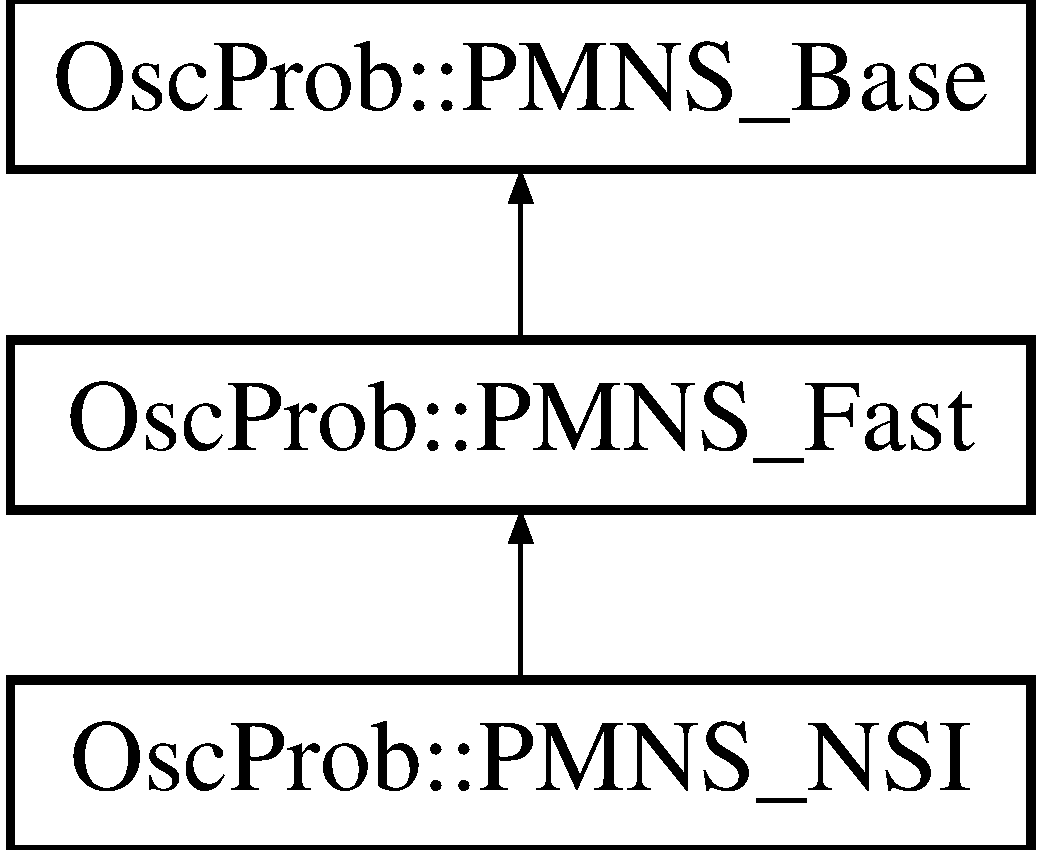
\includegraphics[height=3.000000cm]{classOscProb_1_1PMNS__NSI}
\end{center}
\end{figure}
\subsection*{Public Types}
\begin{DoxyCompactItemize}
\item 
typedef std\+::complex$<$ double $>$ \hyperlink{classOscProb_1_1PMNS__Base_ae86ec4718808ce9d02e5f5b4226714ab}{complex}
\end{DoxyCompactItemize}
\subsection*{Public Member Functions}
\begin{DoxyCompactItemize}
\item 
\hyperlink{classOscProb_1_1PMNS__NSI_ab41e79fb427c7a5662443acad31ce7e9}{P\+M\+N\+S\+\_\+\+N\+SI} ()
\begin{DoxyCompactList}\small\item\em Constructor. \end{DoxyCompactList}\item 
virtual \hyperlink{classOscProb_1_1PMNS__NSI_aad1035cb0fb26994029c25b475ec3bde}{$\sim$\+P\+M\+N\+S\+\_\+\+N\+SI} ()
\begin{DoxyCompactList}\small\item\em Destructor. \end{DoxyCompactList}\item 
virtual void \hyperlink{classOscProb_1_1PMNS__NSI_a87c508149ea36b6de493a6817247a0ea}{Set\+Eps} (int flvi, int flvj, double val, double phase)
\begin{DoxyCompactList}\small\item\em Set any given N\+SI parameter. \end{DoxyCompactList}\item 
virtual \hyperlink{classOscProb_1_1PMNS__Base_ae86ec4718808ce9d02e5f5b4226714ab}{complex} \hyperlink{classOscProb_1_1PMNS__NSI_aac8925ae248f737fe7c3afb12f511534}{Get\+Eps} (int flvi, int flvj)
\begin{DoxyCompactList}\small\item\em Get any given N\+SI parameter. \end{DoxyCompactList}\item 
void \hyperlink{classOscProb_1_1PMNS__NSI_ae8829af10bc4051e8c74c8b1bc81c88c}{Set\+N\+SI} (double eps\+\_\+ee, double eps\+\_\+emu, double eps\+\_\+etau, double eps\+\_\+mumu, double eps\+\_\+mutau, double eps\+\_\+tautau, double delta\+\_\+emu=0, double delta\+\_\+etau=0, double delta\+\_\+mutau=0)
\begin{DoxyCompactList}\small\item\em Set the N\+SI parameters all at once. \end{DoxyCompactList}\item 
virtual void \hyperlink{classOscProb_1_1PMNS__NSI_a13ecb89c4d43924d23833a9e930f50e0}{Set\+Eps\+\_\+ee} (double a)
\begin{DoxyCompactList}\small\item\em Set eps\+\_\+ee parameter. \end{DoxyCompactList}\item 
virtual void \hyperlink{classOscProb_1_1PMNS__NSI_abf049db9904c745f04346d0d1dedf998}{Set\+Eps\+\_\+mumu} (double a)
\begin{DoxyCompactList}\small\item\em Set eps\+\_\+mumu parameter. \end{DoxyCompactList}\item 
virtual void \hyperlink{classOscProb_1_1PMNS__NSI_a5736f3cd792a621dfa844c3fa314cd17}{Set\+Eps\+\_\+tautau} (double a)
\begin{DoxyCompactList}\small\item\em Set eps\+\_\+tautau parameter. \end{DoxyCompactList}\item 
virtual void \hyperlink{classOscProb_1_1PMNS__NSI_ad5fccd151aea7c673c516b8686f8253c}{Set\+Eps\+\_\+emu} (double a, double phi)
\begin{DoxyCompactList}\small\item\em Set eps\+\_\+emu parameter. \end{DoxyCompactList}\item 
virtual void \hyperlink{classOscProb_1_1PMNS__NSI_a73d43e6d267975d1545af922f8e81bb3}{Set\+Eps\+\_\+etau} (double a, double phi)
\begin{DoxyCompactList}\small\item\em Set eps\+\_\+etau parameter. \end{DoxyCompactList}\item 
virtual void \hyperlink{classOscProb_1_1PMNS__NSI_acfb9893697e04fcc25915ffaf8ed137f}{Set\+Eps\+\_\+mutau} (double a, double phi)
\begin{DoxyCompactList}\small\item\em Set eps\+\_\+mutau parameter. \end{DoxyCompactList}\item 
virtual void \hyperlink{classOscProb_1_1PMNS__Fast_ad849b2231d99c5d66fb3ade8efb896e1}{Set\+Mix} (double th12, double th23, double th13, double deltacp)
\begin{DoxyCompactList}\small\item\em Set the all mixing parameters at once. \end{DoxyCompactList}\item 
virtual void \hyperlink{classOscProb_1_1PMNS__Fast_a63733b246e6d2e609ce3de7a65ba5b9f}{Set\+Delta\+Msqrs} (double dm21, double dm32)
\begin{DoxyCompactList}\small\item\em Set both mass-\/splittings at once. \end{DoxyCompactList}\item 
virtual double \hyperlink{classOscProb_1_1PMNS__Base_aec5c399b93261f1962a4b7dbbb44b973}{Prob} (int flvi, int flvf)
\begin{DoxyCompactList}\small\item\em Compute the probability of flvi going to flvf. \end{DoxyCompactList}\item 
virtual double \hyperlink{classOscProb_1_1PMNS__Base_aa3cee10639d5c0879ccb9e78d62128d3}{Prob} (int flvi, int flvf, double E)
\begin{DoxyCompactList}\small\item\em Compute the probability of flvi going to flvf for energy E. \end{DoxyCompactList}\item 
virtual double \hyperlink{classOscProb_1_1PMNS__Base_a6e0a74508d9d6db7be02e242b8467563}{Prob} (int flvi, int flvf, double E, double L)
\begin{DoxyCompactList}\small\item\em Compute the probability of flvi going to flvf for energy E and distance L. \end{DoxyCompactList}\item 
virtual double \hyperlink{classOscProb_1_1PMNS__Base_ac03f754160422e6600da8dbae0f803ed}{Avg\+Prob} (int flvi, int flvf, double E, double dE=0)
\begin{DoxyCompactList}\small\item\em Compute the average probability over a bin of energy. \end{DoxyCompactList}\item 
virtual double \hyperlink{classOscProb_1_1PMNS__Base_ac19a92f4ef428a7333ca8eed76fca637}{Avg\+Prob\+LoE} (int flvi, int flvf, double LoE, double d\+LoE=0)
\begin{DoxyCompactList}\small\item\em Compute the average probability over a bin of L/E. \end{DoxyCompactList}\item 
virtual void \hyperlink{classOscProb_1_1PMNS__Base_ace7875cf6d3bec161a2b7ed2690aec34}{Set\+Angle} (int i, int j, double th)
\begin{DoxyCompactList}\small\item\em Set the mixing angle theta\+\_\+ij. \end{DoxyCompactList}\item 
virtual void \hyperlink{classOscProb_1_1PMNS__Base_a4bef78cfcfc4e70b4ce79cdb8862c0a3}{Set\+Delta} (int i, int j, double delta)
\begin{DoxyCompactList}\small\item\em Set the CP phase delta\+\_\+ij. \end{DoxyCompactList}\item 
virtual void \hyperlink{classOscProb_1_1PMNS__Base_a492243b22fb1b783cd2943f507cff970}{Set\+Dm} (int j, double dm)
\begin{DoxyCompactList}\small\item\em Set the mass-\/splitting dm\+\_\+j1 in e\+V$^\wedge$2. \end{DoxyCompactList}\item 
virtual double \hyperlink{classOscProb_1_1PMNS__Base_acee137091304c919642293ddf015bbc8}{Get\+Angle} (int i, int j)
\begin{DoxyCompactList}\small\item\em Get the mixing angle theta\+\_\+ij. \end{DoxyCompactList}\item 
virtual double \hyperlink{classOscProb_1_1PMNS__Base_adb8dbc91d4286d2e7c8f768c59476241}{Get\+Delta} (int i, int j)
\begin{DoxyCompactList}\small\item\em Get the CP phase delta\+\_\+ij. \end{DoxyCompactList}\item 
virtual double \hyperlink{classOscProb_1_1PMNS__Base_ad26815ac5f4805d1259817e4936e5f8f}{Get\+Dm} (int j)
\begin{DoxyCompactList}\small\item\em Get the mass-\/splitting dm\+\_\+j1 in e\+V$^\wedge$2. \end{DoxyCompactList}\item 
virtual void \hyperlink{classOscProb_1_1PMNS__Base_a4de96ac9b6d1e9b029ab877e57d211ad}{Set\+Std\+Pars} ()
\begin{DoxyCompactList}\small\item\em Set P\+DG 3-\/flavor parameters. \end{DoxyCompactList}\item 
virtual void \hyperlink{classOscProb_1_1PMNS__Base_a95b3b0d0cab5e6a54b5ef99587f837c0}{Set\+Energy} (double E)
\begin{DoxyCompactList}\small\item\em Set the neutrino energy in GeV. \end{DoxyCompactList}\item 
virtual void \hyperlink{classOscProb_1_1PMNS__Base_a717e0348cf762f3961854e332a9b52e0}{Set\+Is\+Nu\+Bar} (bool is\+Nu\+Bar)
\begin{DoxyCompactList}\small\item\em Set the anti-\/neutrino flag. \end{DoxyCompactList}\item 
virtual double \hyperlink{classOscProb_1_1PMNS__Base_acc0d46cc4b8f911b40b807225003bbed}{Get\+Energy} ()
\begin{DoxyCompactList}\small\item\em Get the neutrino energy in GeV. \end{DoxyCompactList}\item 
virtual bool \hyperlink{classOscProb_1_1PMNS__Base_a2f7f2a028dfe7a90fff6b4f757972c2c}{Get\+Is\+Nu\+Bar} ()
\begin{DoxyCompactList}\small\item\em Get the anti-\/neutrino flag. \end{DoxyCompactList}\item 
virtual void \hyperlink{classOscProb_1_1PMNS__Base_ac3b644fd0a56347d304ceca4ae9d8875}{Set\+Path} (\hyperlink{structOscProb_1_1NuPath}{Osc\+Prob\+::\+Nu\+Path} p)
\begin{DoxyCompactList}\small\item\em Set a single path. \end{DoxyCompactList}\item 
virtual void \hyperlink{classOscProb_1_1PMNS__Base_a35b983270613072a3df58b574d80dbfd}{Set\+Path} (double length, double density, double zoa=0.\+5, int layer=0)
\begin{DoxyCompactList}\small\item\em Set a single path. \end{DoxyCompactList}\item 
virtual void \hyperlink{classOscProb_1_1PMNS__Base_a637d19dd850b4246507796526622643c}{Set\+Path} (std\+::vector$<$ \hyperlink{structOscProb_1_1NuPath}{Osc\+Prob\+::\+Nu\+Path} $>$ paths)
\begin{DoxyCompactList}\small\item\em Set a path sequence. \end{DoxyCompactList}\item 
virtual void \hyperlink{classOscProb_1_1PMNS__Base_a887dc9d4dc569ec0cdef3933b4c60efc}{Add\+Path} (\hyperlink{structOscProb_1_1NuPath}{Osc\+Prob\+::\+Nu\+Path} p)
\begin{DoxyCompactList}\small\item\em Add a path to the sequence. \end{DoxyCompactList}\item 
virtual void \hyperlink{classOscProb_1_1PMNS__Base_ab7f89ad9e7e1224adaa59d3c41594cd9}{Add\+Path} (double length, double density, double zoa=0.\+5, int layer=0)
\begin{DoxyCompactList}\small\item\em Add a path to the sequence. \end{DoxyCompactList}\item 
virtual void \hyperlink{classOscProb_1_1PMNS__Base_aefe521239031c418cfaaaa550a6e13bb}{Clear\+Path} ()
\begin{DoxyCompactList}\small\item\em Clear the path vector. \end{DoxyCompactList}\item 
virtual void \hyperlink{classOscProb_1_1PMNS__Base_a6241325b1bd28cafa556daaecbe4ed62}{Set\+Length} (double L)
\begin{DoxyCompactList}\small\item\em Set a single path lentgh in km. \end{DoxyCompactList}\item 
virtual void \hyperlink{classOscProb_1_1PMNS__Base_aa34a40a3b5abda0f252982d9ead3b520}{Set\+Length} (std\+::vector$<$ double $>$ L)
\begin{DoxyCompactList}\small\item\em Set multiple path lengths. \end{DoxyCompactList}\item 
virtual void \hyperlink{classOscProb_1_1PMNS__Base_ac74206f349687da141392c81e2ba6b0d}{Set\+Density} (double rho)
\begin{DoxyCompactList}\small\item\em Set single path density in g/cm$^\wedge$3. \end{DoxyCompactList}\item 
virtual void \hyperlink{classOscProb_1_1PMNS__Base_a858221d5510fe732dc6a101fd305cda0}{Set\+Density} (std\+::vector$<$ double $>$ rho)
\begin{DoxyCompactList}\small\item\em Set multiple path densities. \end{DoxyCompactList}\item 
virtual void \hyperlink{classOscProb_1_1PMNS__Base_a1bf3ea8fd2507fd2fd82d7410ff8f578}{Set\+ZoA} (double zoa)
\begin{DoxyCompactList}\small\item\em Set Z/A value for single path. \end{DoxyCompactList}\item 
virtual void \hyperlink{classOscProb_1_1PMNS__Base_a8495f8a320e1a21965e6a64aec92ad2a}{Set\+ZoA} (std\+::vector$<$ double $>$ zoa)
\begin{DoxyCompactList}\small\item\em Set multiple path Z/A values. \end{DoxyCompactList}\item 
virtual void \hyperlink{classOscProb_1_1PMNS__Base_a904e580edf89fb98bf9a6397739b4ebe}{Set\+Layers} (std\+::vector$<$ int $>$ lay)
\begin{DoxyCompactList}\small\item\em Set multiple path layer indices. \end{DoxyCompactList}\item 
virtual void \hyperlink{classOscProb_1_1PMNS__Base_add6533a9fc9acdfc7ae258b62570d78d}{Set\+Std\+Path} ()
\begin{DoxyCompactList}\small\item\em Set standard neutrino path. \end{DoxyCompactList}\item 
virtual std\+::vector$<$ \hyperlink{structOscProb_1_1NuPath}{Osc\+Prob\+::\+Nu\+Path} $>$ \hyperlink{classOscProb_1_1PMNS__Base_ac8e196f2e85a2b1caaf705073ee95a5c}{Get\+Path} ()
\begin{DoxyCompactList}\small\item\em Get the neutrino path sequence. \end{DoxyCompactList}\item 
virtual std\+::vector$<$ double $>$ \hyperlink{classOscProb_1_1PMNS__Base_a9eac8d768c1424755ee41f7e783af179}{Get\+Sample\+Points} (double LoE, double d\+LoE)
\begin{DoxyCompactList}\small\item\em Compute the sample points for a bin of L/E with width d\+LoE. \end{DoxyCompactList}\end{DoxyCompactItemize}
\subsection*{Protected Member Functions}
\begin{DoxyCompactItemize}
\item 
virtual void \hyperlink{classOscProb_1_1PMNS__NSI_ab5c4f4644fbedb8835f6336c553805ce}{Update\+Ham} ()
\begin{DoxyCompactList}\small\item\em Build the full Hamiltonian. \end{DoxyCompactList}\item 
virtual void \hyperlink{classOscProb_1_1PMNS__Fast_a8a0828401591e88c60e0051fbfe02d5e}{Solve\+Ham} ()
\begin{DoxyCompactList}\small\item\em Solve the full Hamiltonian for eigenvectors and eigenvalues. \end{DoxyCompactList}\item 
virtual void \hyperlink{classOscProb_1_1PMNS__Fast_a76dd5a761df8689c502b28ad0391f9e2}{Set\+Vacuum\+Eigensystem} ()
\begin{DoxyCompactList}\small\item\em Set the eigensystem to the analytic solution of the vacuum Hamiltonian. \end{DoxyCompactList}\item 
virtual void \hyperlink{classOscProb_1_1PMNS__Base_adf23b569112f9f9e0e592f01d79a5f3d}{Initialize\+Vectors} ()
\begin{DoxyCompactList}\small\item\em Initialize all member vectors with zeros. \end{DoxyCompactList}\item 
virtual void \hyperlink{classOscProb_1_1PMNS__Base_a986e6ebef09a7e2eb7fee16a4c2c834d}{Set\+Cur\+Path} (\hyperlink{structOscProb_1_1NuPath}{Osc\+Prob\+::\+Nu\+Path} p)
\begin{DoxyCompactList}\small\item\em Set the path currently in use by the class. \end{DoxyCompactList}\item 
virtual void \hyperlink{classOscProb_1_1PMNS__Base_aba565962a440d14bee7a2a96d2eca2c5}{Set\+Att} (double att, int idx)
\begin{DoxyCompactList}\small\item\em Set one of the path attributes. \end{DoxyCompactList}\item 
virtual void \hyperlink{classOscProb_1_1PMNS__Base_aa001479b5f5828c3d16ed087f96ecbcc}{Set\+Att} (std\+::vector$<$ double $>$ att, int idx)
\begin{DoxyCompactList}\small\item\em Set all values of a path attribute. \end{DoxyCompactList}\item 
virtual void \hyperlink{classOscProb_1_1PMNS__Base_aae18afd69074211335f49ec40e6011b9}{RotateH} (int i, int j)
\begin{DoxyCompactList}\small\item\em Rotate the Hamiltonian by theta\+\_\+ij and delta\+\_\+ij. \end{DoxyCompactList}\item 
virtual void \hyperlink{classOscProb_1_1PMNS__Base_ad0faf5eae755afb1baa1fcd5ffebad41}{Build\+Hms} ()
\begin{DoxyCompactList}\small\item\em Build the matrix of masses squared. \end{DoxyCompactList}\item 
virtual void \hyperlink{classOscProb_1_1PMNS__Base_ac0d4bf8ff1318ef96d3dafa62e0cec25}{Reset\+To\+Flavour} (int flv)
\begin{DoxyCompactList}\small\item\em Reset neutrino state to pure flavour flv. \end{DoxyCompactList}\item 
virtual void \hyperlink{classOscProb_1_1PMNS__Base_accb08503acc162188041d7a96a280462}{Propagate\+Path} (\hyperlink{structOscProb_1_1NuPath}{Osc\+Prob\+::\+Nu\+Path} p)
\begin{DoxyCompactList}\small\item\em Propagate neutrino through a single path. \end{DoxyCompactList}\item 
virtual void \hyperlink{classOscProb_1_1PMNS__Base_a054e3a8b05b9a958b6fa416e4a835e3e}{Propagate} ()
\begin{DoxyCompactList}\small\item\em Propagate neutrino through full path. \end{DoxyCompactList}\item 
virtual double \hyperlink{classOscProb_1_1PMNS__Base_a0dc4d45bc3d7e03b9abbf5b4e100cc22}{P} (int flv)
\begin{DoxyCompactList}\small\item\em Return the probability of final state in flavour flv. \end{DoxyCompactList}\end{DoxyCompactItemize}
\subsection*{Protected Attributes}
\begin{DoxyCompactItemize}
\item 
\hyperlink{classOscProb_1_1PMNS__Base_ae86ec4718808ce9d02e5f5b4226714ab}{complex} \hyperlink{classOscProb_1_1PMNS__NSI_a7e2f0a3fdc633f68523c9de0ce76e67d}{f\+Eps} \mbox{[}3\mbox{]}\mbox{[}3\mbox{]}
\begin{DoxyCompactList}\small\item\em Stores each N\+SI parameter. \end{DoxyCompactList}\item 
\hyperlink{classOscProb_1_1PMNS__Base_ae86ec4718808ce9d02e5f5b4226714ab}{complex} \hyperlink{classOscProb_1_1PMNS__Fast_aab37f2a7f59ab7026a8a21a561115dd0}{f\+Ham} \mbox{[}3\mbox{]}\mbox{[}3\mbox{]}
\begin{DoxyCompactList}\small\item\em The full hamiltonian. \end{DoxyCompactList}\item 
int \hyperlink{classOscProb_1_1PMNS__Base_a24bb74bed63569dfe88b18fa6a08060e}{f\+Num\+Nus}
\begin{DoxyCompactList}\small\item\em Number of neutrino flavours. \end{DoxyCompactList}\item 
std\+::vector$<$ double $>$ \hyperlink{classOscProb_1_1PMNS__Base_a406a31c3b5d620e5a0cace5b411f9f70}{f\+Dm}
\begin{DoxyCompactList}\small\item\em m$^\wedge$2\+\_\+i -\/ m$^\wedge$2\+\_\+1 in vacuum \end{DoxyCompactList}\item 
std\+::vector$<$ std\+::vector$<$ double $>$ $>$ \hyperlink{classOscProb_1_1PMNS__Base_a1976887cd658dd86b2336c181f1470b4}{f\+Theta}
\begin{DoxyCompactList}\small\item\em theta\mbox{[}i\mbox{]}\mbox{[}j\mbox{]} mixing angle \end{DoxyCompactList}\item 
std\+::vector$<$ std\+::vector$<$ double $>$ $>$ \hyperlink{classOscProb_1_1PMNS__Base_ab2a5fa40e689b221c8a7d2c17213810d}{f\+Delta}
\begin{DoxyCompactList}\small\item\em delta\mbox{[}i\mbox{]}\mbox{[}j\mbox{]} CP violating phase \end{DoxyCompactList}\item 
std\+::vector$<$ \hyperlink{classOscProb_1_1PMNS__Base_ae86ec4718808ce9d02e5f5b4226714ab}{complex} $>$ \hyperlink{classOscProb_1_1PMNS__Base_ad38a7107c3ab393591fd5ba21658300b}{f\+Nu\+State}
\begin{DoxyCompactList}\small\item\em The neutrino current state. \end{DoxyCompactList}\item 
std\+::vector$<$ std\+::vector$<$ \hyperlink{classOscProb_1_1PMNS__Base_ae86ec4718808ce9d02e5f5b4226714ab}{complex} $>$ $>$ \hyperlink{classOscProb_1_1PMNS__Base_adf5901166216e8c7a5cff2092952f473}{f\+Hms}
\begin{DoxyCompactList}\small\item\em matrix H$\ast$2E in e\+V$^\wedge$2 \end{DoxyCompactList}\item 
std\+::vector$<$ \hyperlink{classOscProb_1_1PMNS__Base_ae86ec4718808ce9d02e5f5b4226714ab}{complex} $>$ \hyperlink{classOscProb_1_1PMNS__Base_a2fcb59d7c533e4cd963b1890e504d3dc}{f\+Phases}
\begin{DoxyCompactList}\small\item\em Buffer for oscillation phases. \end{DoxyCompactList}\item 
std\+::vector$<$ \hyperlink{classOscProb_1_1PMNS__Base_ae86ec4718808ce9d02e5f5b4226714ab}{complex} $>$ \hyperlink{classOscProb_1_1PMNS__Base_a53f912c6e4a17035a6c0c11fd63b5f14}{f\+Buffer}
\begin{DoxyCompactList}\small\item\em Buffer for neutrino state tranformations. \end{DoxyCompactList}\item 
std\+::vector$<$ double $>$ \hyperlink{classOscProb_1_1PMNS__Base_a6319c34d7decbb9d7d6da279c06e8c2d}{f\+Eval}
\begin{DoxyCompactList}\small\item\em Eigenvalues of the Hamiltonian. \end{DoxyCompactList}\item 
std\+::vector$<$ std\+::vector$<$ \hyperlink{classOscProb_1_1PMNS__Base_ae86ec4718808ce9d02e5f5b4226714ab}{complex} $>$ $>$ \hyperlink{classOscProb_1_1PMNS__Base_a093e7bd31d4ef52ed52df414e12c1d17}{f\+Evec}
\begin{DoxyCompactList}\small\item\em Eigenvectors of the Hamiltonian. \end{DoxyCompactList}\item 
double \hyperlink{classOscProb_1_1PMNS__Base_a2800af6d436972f3e900867790c046b0}{f\+Energy}
\begin{DoxyCompactList}\small\item\em Neutrino energy. \end{DoxyCompactList}\item 
bool \hyperlink{classOscProb_1_1PMNS__Base_a0ebaeaefab36a3ff381c6293faedfdd6}{f\+Is\+Nu\+Bar}
\begin{DoxyCompactList}\small\item\em Anti-\/neutrino flag. \end{DoxyCompactList}\item 
std\+::vector$<$ \hyperlink{structOscProb_1_1NuPath}{Osc\+Prob\+::\+Nu\+Path} $>$ \hyperlink{classOscProb_1_1PMNS__Base_a69db9d57e12fc7cbe0431bc6c18fac93}{f\+Nu\+Paths}
\begin{DoxyCompactList}\small\item\em Vector of neutrino paths. \end{DoxyCompactList}\item 
\hyperlink{structOscProb_1_1NuPath}{Osc\+Prob\+::\+Nu\+Path} \hyperlink{classOscProb_1_1PMNS__Base_a849437aa8891fe042e86886ce8f81c6e}{f\+Path}
\begin{DoxyCompactList}\small\item\em Current neutrino path. \end{DoxyCompactList}\item 
bool \hyperlink{classOscProb_1_1PMNS__Base_a9ac3cadeac8db1b90f3152f476244780}{f\+Built\+Hms}
\begin{DoxyCompactList}\small\item\em Tag to avoid rebuilding Hms. \end{DoxyCompactList}\item 
bool \hyperlink{classOscProb_1_1PMNS__Base_a6dc5cd010d2d70b2324745b4e53e9839}{f\+Got\+ES}
\begin{DoxyCompactList}\small\item\em Tag to avoid recalculating eigensystem. \end{DoxyCompactList}\end{DoxyCompactItemize}
\subsection*{Static Protected Attributes}
\begin{DoxyCompactItemize}
\item 
static const \hyperlink{classOscProb_1_1PMNS__Base_ae86ec4718808ce9d02e5f5b4226714ab}{complex} \hyperlink{classOscProb_1_1PMNS__Base_a5c31ed4593cf95feb36fb80c1850d25e}{zero}
\begin{DoxyCompactList}\small\item\em zero in complex \end{DoxyCompactList}\item 
static const \hyperlink{classOscProb_1_1PMNS__Base_ae86ec4718808ce9d02e5f5b4226714ab}{complex} \hyperlink{classOscProb_1_1PMNS__Base_ab64aab27448a5aca27565c991a9d173e}{one}
\begin{DoxyCompactList}\small\item\em one in complex \end{DoxyCompactList}\item 
static const double \hyperlink{classOscProb_1_1PMNS__Base_a382ddd7b76ca89b43f22614a2ea7327b}{k\+Km2eV} = 1.\+0 / 1.\+973269788e-\/10
\begin{DoxyCompactList}\small\item\em km to e\+V$^\wedge$-\/1 \end{DoxyCompactList}\item 
static const double \hyperlink{classOscProb_1_1PMNS__Base_a326fc5016d7dd7ce05682c06cdcb6d94}{k\+K2} = 1e-\/3 $\ast$ k\+N\+A / pow(k\+Km2e\+V,3)
\begin{DoxyCompactList}\small\item\em mol/\+Ge\+V$^\wedge$2/cm$^\wedge$3 to eV \end{DoxyCompactList}\item 
static const double \hyperlink{classOscProb_1_1PMNS__Base_ad36a0a6bf58d6ec093d3947784bd89e9}{k\+Ge\+V2eV} = 1.\+0e+09
\begin{DoxyCompactList}\small\item\em GeV to eV. \end{DoxyCompactList}\item 
static const double \hyperlink{classOscProb_1_1PMNS__Base_a69355e770b89e99437c2b8a66e48eeb9}{k\+NA} = 6.\+022140857e23
\begin{DoxyCompactList}\small\item\em Avogadro constant. \end{DoxyCompactList}\item 
static const double \hyperlink{classOscProb_1_1PMNS__Base_a7f26a3456128234b2ae6cc9141a6532f}{k\+Gf} = 1.\+1663787e-\/05
\begin{DoxyCompactList}\small\item\em G\+\_\+F in units of Ge\+V$^\wedge$-\/2. \end{DoxyCompactList}\end{DoxyCompactItemize}


\subsection{Detailed Description}
This class expands the \hyperlink{classOscProb_1_1PMNS__Fast}{P\+M\+N\+S\+\_\+\+Fast} class including a general matter potential matrix describing Non-\/\+Standard Interactions (N\+SI).

The matter potential is parametrized by dimensionless quantities epsilon which quantify the intensity of the N\+SI with respect to the standard matter effects from coherent forward scattering with electrons.

\begin{DoxySeeAlso}{See also}
\hyperlink{classOscProb_1_1PMNS__Fast}{P\+M\+N\+S\+\_\+\+Fast}
\end{DoxySeeAlso}
\begin{DoxyAuthor}{Author}
coelho@lal.\+in2p3.\+fr 
\end{DoxyAuthor}


Definition at line 25 of file P\+M\+N\+S\+\_\+\+N\+S\+I.\+h.



\subsection{Member Typedef Documentation}
\mbox{\Hypertarget{classOscProb_1_1PMNS__Base_ae86ec4718808ce9d02e5f5b4226714ab}\label{classOscProb_1_1PMNS__Base_ae86ec4718808ce9d02e5f5b4226714ab}} 
\index{Osc\+Prob\+::\+P\+M\+N\+S\+\_\+\+N\+SI@{Osc\+Prob\+::\+P\+M\+N\+S\+\_\+\+N\+SI}!complex@{complex}}
\index{complex@{complex}!Osc\+Prob\+::\+P\+M\+N\+S\+\_\+\+N\+SI@{Osc\+Prob\+::\+P\+M\+N\+S\+\_\+\+N\+SI}}
\subsubsection{\texorpdfstring{complex}{complex}}
{\footnotesize\ttfamily typedef std\+::complex$<$double$>$ \hyperlink{classOscProb_1_1PMNS__Base_ae86ec4718808ce9d02e5f5b4226714ab}{Osc\+Prob\+::\+P\+M\+N\+S\+\_\+\+Base\+::complex}\hspace{0.3cm}{\ttfamily [inherited]}}



Definition at line 104 of file P\+M\+N\+S\+\_\+\+Base.\+h.



\subsection{Constructor \& Destructor Documentation}
\mbox{\Hypertarget{classOscProb_1_1PMNS__NSI_ab41e79fb427c7a5662443acad31ce7e9}\label{classOscProb_1_1PMNS__NSI_ab41e79fb427c7a5662443acad31ce7e9}} 
\index{Osc\+Prob\+::\+P\+M\+N\+S\+\_\+\+N\+SI@{Osc\+Prob\+::\+P\+M\+N\+S\+\_\+\+N\+SI}!P\+M\+N\+S\+\_\+\+N\+SI@{P\+M\+N\+S\+\_\+\+N\+SI}}
\index{P\+M\+N\+S\+\_\+\+N\+SI@{P\+M\+N\+S\+\_\+\+N\+SI}!Osc\+Prob\+::\+P\+M\+N\+S\+\_\+\+N\+SI@{Osc\+Prob\+::\+P\+M\+N\+S\+\_\+\+N\+SI}}
\subsubsection{\texorpdfstring{P\+M\+N\+S\+\_\+\+N\+S\+I()}{PMNS\_NSI()}}
{\footnotesize\ttfamily P\+M\+N\+S\+\_\+\+N\+S\+I\+::\+P\+M\+N\+S\+\_\+\+N\+SI (\begin{DoxyParamCaption}{ }\end{DoxyParamCaption})}

Constructor. \begin{DoxySeeAlso}{See also}
\hyperlink{classOscProb_1_1PMNS__Base_aa53e83b03a9cf4bdfa0a07136bd17a79}{P\+M\+N\+S\+\_\+\+Base\+::\+P\+M\+N\+S\+\_\+\+Base}
\end{DoxySeeAlso}
This class is restricted to 3 neutrino flavours. 

Definition at line 29 of file P\+M\+N\+S\+\_\+\+N\+S\+I.\+cxx.



References Set\+N\+S\+I(), and Osc\+Prob\+::\+P\+M\+N\+S\+\_\+\+Base\+::\+Set\+Std\+Path().


\begin{DoxyCode}
29                    : \hyperlink{classOscProb_1_1PMNS__Fast_a2bbac744bf63753105d766a860af7c0d}{PMNS\_Fast}(), \hyperlink{classOscProb_1_1PMNS__NSI_a7e2f0a3fdc633f68523c9de0ce76e67d}{fEps}()
30 \{
31   \hyperlink{classOscProb_1_1PMNS__Base_add6533a9fc9acdfc7ae258b62570d78d}{SetStdPath}();
32   \hyperlink{classOscProb_1_1PMNS__NSI_ae8829af10bc4051e8c74c8b1bc81c88c}{SetNSI}(0.,0.,0.,0.,0.,0.,0.,0.,0.);
33 \}
\end{DoxyCode}
\mbox{\Hypertarget{classOscProb_1_1PMNS__NSI_aad1035cb0fb26994029c25b475ec3bde}\label{classOscProb_1_1PMNS__NSI_aad1035cb0fb26994029c25b475ec3bde}} 
\index{Osc\+Prob\+::\+P\+M\+N\+S\+\_\+\+N\+SI@{Osc\+Prob\+::\+P\+M\+N\+S\+\_\+\+N\+SI}!````~P\+M\+N\+S\+\_\+\+N\+SI@{$\sim$\+P\+M\+N\+S\+\_\+\+N\+SI}}
\index{````~P\+M\+N\+S\+\_\+\+N\+SI@{$\sim$\+P\+M\+N\+S\+\_\+\+N\+SI}!Osc\+Prob\+::\+P\+M\+N\+S\+\_\+\+N\+SI@{Osc\+Prob\+::\+P\+M\+N\+S\+\_\+\+N\+SI}}
\subsubsection{\texorpdfstring{$\sim$\+P\+M\+N\+S\+\_\+\+N\+S\+I()}{~PMNS\_NSI()}}
{\footnotesize\ttfamily P\+M\+N\+S\+\_\+\+N\+S\+I\+::$\sim$\+P\+M\+N\+S\+\_\+\+N\+SI (\begin{DoxyParamCaption}{ }\end{DoxyParamCaption})\hspace{0.3cm}{\ttfamily [virtual]}}

Nothing to clean. 

Definition at line 39 of file P\+M\+N\+S\+\_\+\+N\+S\+I.\+cxx.


\begin{DoxyCode}
39 \{\}
\end{DoxyCode}


\subsection{Member Function Documentation}
\mbox{\Hypertarget{classOscProb_1_1PMNS__Base_a887dc9d4dc569ec0cdef3933b4c60efc}\label{classOscProb_1_1PMNS__Base_a887dc9d4dc569ec0cdef3933b4c60efc}} 
\index{Osc\+Prob\+::\+P\+M\+N\+S\+\_\+\+N\+SI@{Osc\+Prob\+::\+P\+M\+N\+S\+\_\+\+N\+SI}!Add\+Path@{Add\+Path}}
\index{Add\+Path@{Add\+Path}!Osc\+Prob\+::\+P\+M\+N\+S\+\_\+\+N\+SI@{Osc\+Prob\+::\+P\+M\+N\+S\+\_\+\+N\+SI}}
\subsubsection{\texorpdfstring{Add\+Path()}{AddPath()}\hspace{0.1cm}{\footnotesize\ttfamily [1/2]}}
{\footnotesize\ttfamily void P\+M\+N\+S\+\_\+\+Base\+::\+Add\+Path (\begin{DoxyParamCaption}\item[{\hyperlink{structOscProb_1_1NuPath}{Osc\+Prob\+::\+Nu\+Path}}]{p }\end{DoxyParamCaption})\hspace{0.3cm}{\ttfamily [virtual]}, {\ttfamily [inherited]}}

Add a path to the sequence. 
\begin{DoxyParams}{Parameters}
{\em p} & -\/ A neutrino path segment \\
\hline
\end{DoxyParams}


Definition at line 260 of file P\+M\+N\+S\+\_\+\+Base.\+cxx.



References Osc\+Prob\+::\+P\+M\+N\+S\+\_\+\+Base\+::f\+Nu\+Paths.



Referenced by Osc\+Prob\+::\+P\+M\+N\+S\+\_\+\+Base\+::\+Add\+Path(), Osc\+Prob\+::\+P\+M\+N\+S\+\_\+\+Base\+::\+Set\+Att(), and Osc\+Prob\+::\+P\+M\+N\+S\+\_\+\+Base\+::\+Set\+Path().


\begin{DoxyCode}
260                                \{
261 
262   \hyperlink{classOscProb_1_1PMNS__Base_a69db9d57e12fc7cbe0431bc6c18fac93}{fNuPaths}.push\_back(p);
263 
264 \}
\end{DoxyCode}
\mbox{\Hypertarget{classOscProb_1_1PMNS__Base_ab7f89ad9e7e1224adaa59d3c41594cd9}\label{classOscProb_1_1PMNS__Base_ab7f89ad9e7e1224adaa59d3c41594cd9}} 
\index{Osc\+Prob\+::\+P\+M\+N\+S\+\_\+\+N\+SI@{Osc\+Prob\+::\+P\+M\+N\+S\+\_\+\+N\+SI}!Add\+Path@{Add\+Path}}
\index{Add\+Path@{Add\+Path}!Osc\+Prob\+::\+P\+M\+N\+S\+\_\+\+N\+SI@{Osc\+Prob\+::\+P\+M\+N\+S\+\_\+\+N\+SI}}
\subsubsection{\texorpdfstring{Add\+Path()}{AddPath()}\hspace{0.1cm}{\footnotesize\ttfamily [2/2]}}
{\footnotesize\ttfamily void P\+M\+N\+S\+\_\+\+Base\+::\+Add\+Path (\begin{DoxyParamCaption}\item[{double}]{length,  }\item[{double}]{density,  }\item[{double}]{zoa = {\ttfamily 0.5},  }\item[{int}]{layer = {\ttfamily 0} }\end{DoxyParamCaption})\hspace{0.3cm}{\ttfamily [virtual]}, {\ttfamily [inherited]}}

Add a path to the sequence defining attributes directly. 
\begin{DoxyParams}{Parameters}
{\em length} & -\/ The length of the path segment in km \\
\hline
{\em density} & -\/ The density of the path segment in g/cm$^\wedge$3 \\
\hline
{\em zoa} & -\/ The effective Z/A of the path segment \\
\hline
{\em layer} & -\/ An index to identify the layer type (e.\+g. earth inner core) \\
\hline
\end{DoxyParams}


Definition at line 274 of file P\+M\+N\+S\+\_\+\+Base.\+cxx.



References Osc\+Prob\+::\+P\+M\+N\+S\+\_\+\+Base\+::\+Add\+Path().


\begin{DoxyCode}
274                                                                            \{
275 
276   \hyperlink{classOscProb_1_1PMNS__Base_a887dc9d4dc569ec0cdef3933b4c60efc}{AddPath}(\hyperlink{structOscProb_1_1NuPath}{NuPath}(length, density, zoa, layer));
277 
278 \}
\end{DoxyCode}
\mbox{\Hypertarget{classOscProb_1_1PMNS__Base_ac03f754160422e6600da8dbae0f803ed}\label{classOscProb_1_1PMNS__Base_ac03f754160422e6600da8dbae0f803ed}} 
\index{Osc\+Prob\+::\+P\+M\+N\+S\+\_\+\+N\+SI@{Osc\+Prob\+::\+P\+M\+N\+S\+\_\+\+N\+SI}!Avg\+Prob@{Avg\+Prob}}
\index{Avg\+Prob@{Avg\+Prob}!Osc\+Prob\+::\+P\+M\+N\+S\+\_\+\+N\+SI@{Osc\+Prob\+::\+P\+M\+N\+S\+\_\+\+N\+SI}}
\subsubsection{\texorpdfstring{Avg\+Prob()}{AvgProb()}}
{\footnotesize\ttfamily double P\+M\+N\+S\+\_\+\+Base\+::\+Avg\+Prob (\begin{DoxyParamCaption}\item[{int}]{flvi,  }\item[{int}]{flvf,  }\item[{double}]{E,  }\item[{double}]{dE = {\ttfamily 0} }\end{DoxyParamCaption})\hspace{0.3cm}{\ttfamily [virtual]}, {\ttfamily [inherited]}}

Compute the average probability of flvi going to flvf over a bin of energy E with width dE.

This gets transformed into L/E, since the oscillation terms have arguments linear in L/E and not E.

This function currently only works for single paths.

Flavours are\+: 
\begin{DoxyPre}
  0 = nue, 1 = numu, 2 = nutau
  3 = sterile\_1, 4 = sterile\_2, etc.
\end{DoxyPre}
 
\begin{DoxyParams}{Parameters}
{\em flvi} & -\/ The neutrino starting flavour. \\
\hline
{\em flvf} & -\/ The neutrino final flavour. \\
\hline
{\em E} & -\/ The neutrino energy in the bin center in GeV \\
\hline
{\em dE} & -\/ The energy bin width in GeV\\
\hline
\end{DoxyParams}
\begin{DoxyReturn}{Returns}
Average neutrino oscillation probability 
\end{DoxyReturn}


Definition at line 1084 of file P\+M\+N\+S\+\_\+\+Base.\+cxx.



References Osc\+Prob\+::\+P\+M\+N\+S\+\_\+\+Base\+::\+Avg\+Prob\+Lo\+E(), Osc\+Prob\+::\+P\+M\+N\+S\+\_\+\+Base\+::f\+Nu\+Paths, Osc\+Prob\+::\+P\+M\+N\+S\+\_\+\+Base\+::f\+Path, Osc\+Prob\+::\+Nu\+Path\+::length, Osc\+Prob\+::\+P\+M\+N\+S\+\_\+\+Base\+::\+Prob(), and Osc\+Prob\+::\+P\+M\+N\+S\+\_\+\+Base\+::\+Set\+Cur\+Path().


\begin{DoxyCode}
1085 \{
1086 
1087   \textcolor{comment}{// Do nothing if energy is not positive}
1088   \textcolor{keywordflow}{if}(E<=0) \textcolor{keywordflow}{return} 0;
1089 
1090   \textcolor{keywordflow}{if}(\hyperlink{classOscProb_1_1PMNS__Base_a69db9d57e12fc7cbe0431bc6c18fac93}{fNuPaths}.empty()) \textcolor{keywordflow}{return} 0;
1091 
1092   \textcolor{keywordflow}{if}(\hyperlink{classOscProb_1_1PMNS__Base_a69db9d57e12fc7cbe0431bc6c18fac93}{fNuPaths}.size() != 1)\{
1093     cout << \textcolor{stringliteral}{"ERROR: AvgProb not implemented for multiple paths."} << endl;
1094     cout << \textcolor{stringliteral}{"       Returning probability at bin center."} << endl;
1095     \textcolor{keywordflow}{return} \hyperlink{classOscProb_1_1PMNS__Base_aec5c399b93261f1962a4b7dbbb44b973}{Prob}(flvi, flvf, E);
1096   \}
1097 
1098   \textcolor{comment}{// Don't average zero width}
1099   \textcolor{keywordflow}{if}(dE<=0) \textcolor{keywordflow}{return} \hyperlink{classOscProb_1_1PMNS__Base_aec5c399b93261f1962a4b7dbbb44b973}{Prob}(flvi, flvf, E);
1100 
1101   \textcolor{comment}{// Make sure fPath is set}
1102   \hyperlink{classOscProb_1_1PMNS__Base_a986e6ebef09a7e2eb7fee16a4c2c834d}{SetCurPath}(\hyperlink{classOscProb_1_1PMNS__Base_a69db9d57e12fc7cbe0431bc6c18fac93}{fNuPaths}[0]);
1103 
1104   \textcolor{comment}{// Define L/E variables}
1105   \textcolor{keywordtype}{double} LoE = 0;
1106   \textcolor{keywordtype}{double} dLoE = 0;
1107 
1108   \textcolor{comment}{// Set a minimum energy}
1109   \textcolor{keywordtype}{double} minE = 0.1 * E;
1110 
1111   \textcolor{comment}{// Transform range to L/E}
1112   \textcolor{comment}{// Full range if low edge > minE}
1113   \textcolor{keywordflow}{if}(E-dE/2 > minE)\{
1114     LoE = 0.5 * (\hyperlink{classOscProb_1_1PMNS__Base_a849437aa8891fe042e86886ce8f81c6e}{fPath}.\hyperlink{structOscProb_1_1NuPath_af22660894b6e25cf835500381b155557}{length}/(E-dE/2) + \hyperlink{classOscProb_1_1PMNS__Base_a849437aa8891fe042e86886ce8f81c6e}{fPath}.\hyperlink{structOscProb_1_1NuPath_af22660894b6e25cf835500381b155557}{length}/(E+dE/2));
1115     dLoE = \hyperlink{classOscProb_1_1PMNS__Base_a849437aa8891fe042e86886ce8f81c6e}{fPath}.\hyperlink{structOscProb_1_1NuPath_af22660894b6e25cf835500381b155557}{length}/(E-dE/2) - \hyperlink{classOscProb_1_1PMNS__Base_a849437aa8891fe042e86886ce8f81c6e}{fPath}.\hyperlink{structOscProb_1_1NuPath_af22660894b6e25cf835500381b155557}{length}/(E+dE/2);
1116   \}
1117   \textcolor{comment}{// Else start at minE}
1118   \textcolor{keywordflow}{else}\{
1119     LoE = 0.5 * (\hyperlink{classOscProb_1_1PMNS__Base_a849437aa8891fe042e86886ce8f81c6e}{fPath}.\hyperlink{structOscProb_1_1NuPath_af22660894b6e25cf835500381b155557}{length}/minE + \hyperlink{classOscProb_1_1PMNS__Base_a849437aa8891fe042e86886ce8f81c6e}{fPath}.\hyperlink{structOscProb_1_1NuPath_af22660894b6e25cf835500381b155557}{length}/(E+dE/2));
1120     dLoE = \hyperlink{classOscProb_1_1PMNS__Base_a849437aa8891fe042e86886ce8f81c6e}{fPath}.\hyperlink{structOscProb_1_1NuPath_af22660894b6e25cf835500381b155557}{length}/minE - \hyperlink{classOscProb_1_1PMNS__Base_a849437aa8891fe042e86886ce8f81c6e}{fPath}.\hyperlink{structOscProb_1_1NuPath_af22660894b6e25cf835500381b155557}{length}/(E+dE/2);
1121   \}
1122 
1123   \textcolor{comment}{// Compute average in LoE}
1124   \textcolor{keywordflow}{return} \hyperlink{classOscProb_1_1PMNS__Base_ac19a92f4ef428a7333ca8eed76fca637}{AvgProbLoE}(flvi, flvf, LoE, dLoE);
1125 
1126 \}
\end{DoxyCode}
\mbox{\Hypertarget{classOscProb_1_1PMNS__Base_ac19a92f4ef428a7333ca8eed76fca637}\label{classOscProb_1_1PMNS__Base_ac19a92f4ef428a7333ca8eed76fca637}} 
\index{Osc\+Prob\+::\+P\+M\+N\+S\+\_\+\+N\+SI@{Osc\+Prob\+::\+P\+M\+N\+S\+\_\+\+N\+SI}!Avg\+Prob\+LoE@{Avg\+Prob\+LoE}}
\index{Avg\+Prob\+LoE@{Avg\+Prob\+LoE}!Osc\+Prob\+::\+P\+M\+N\+S\+\_\+\+N\+SI@{Osc\+Prob\+::\+P\+M\+N\+S\+\_\+\+N\+SI}}
\subsubsection{\texorpdfstring{Avg\+Prob\+Lo\+E()}{AvgProbLoE()}}
{\footnotesize\ttfamily double P\+M\+N\+S\+\_\+\+Base\+::\+Avg\+Prob\+LoE (\begin{DoxyParamCaption}\item[{int}]{flvi,  }\item[{int}]{flvf,  }\item[{double}]{LoE,  }\item[{double}]{d\+LoE = {\ttfamily 0} }\end{DoxyParamCaption})\hspace{0.3cm}{\ttfamily [virtual]}, {\ttfamily [inherited]}}

Compute the average probability of flvi going to flvf over a bin of L/E with width d\+LoE.

The probabilities are weighted by (L/E)$^\wedge$-\/2 so that event density is flat in energy. This avoids giving too much weight to low energies. Better approximations would be achieved if we used an interpolated event density.

This function currently only works for single paths.

Flavours are\+: 
\begin{DoxyPre}
  0 = nue, 1 = numu, 2 = nutau
  3 = sterile\_1, 4 = sterile\_2, etc.
\end{DoxyPre}
 
\begin{DoxyParams}{Parameters}
{\em flvi} & -\/ The neutrino starting flavour. \\
\hline
{\em flvf} & -\/ The neutrino final flavour. \\
\hline
{\em LoE} & -\/ The neutrino L/E value in the bin center in km/\+GeV \\
\hline
{\em d\+LoE} & -\/ The L/E bin width in km/\+GeV\\
\hline
\end{DoxyParams}
\begin{DoxyReturn}{Returns}
Average neutrino oscillation probability 
\end{DoxyReturn}


Definition at line 1152 of file P\+M\+N\+S\+\_\+\+Base.\+cxx.



References Osc\+Prob\+::\+P\+M\+N\+S\+\_\+\+Base\+::f\+Nu\+Paths, Osc\+Prob\+::\+P\+M\+N\+S\+\_\+\+Base\+::f\+Path, Osc\+Prob\+::\+P\+M\+N\+S\+\_\+\+Base\+::\+Get\+Sample\+Points(), Osc\+Prob\+::\+Nu\+Path\+::length, Osc\+Prob\+::\+P\+M\+N\+S\+\_\+\+Base\+::\+Prob(), Osc\+Prob\+::\+P\+M\+N\+S\+\_\+\+Base\+::\+Set\+Cur\+Path(), and Osc\+Prob\+::\+P\+M\+N\+S\+\_\+\+Base\+::\+Set\+Energy().



Referenced by Osc\+Prob\+::\+P\+M\+N\+S\+\_\+\+Base\+::\+Avg\+Prob().


\begin{DoxyCode}
1153 \{
1154 
1155   \textcolor{comment}{// Do nothing if L/E is not positive}
1156   \textcolor{keywordflow}{if}(LoE<=0) \textcolor{keywordflow}{return} 0;
1157 
1158   \textcolor{keywordflow}{if}(\hyperlink{classOscProb_1_1PMNS__Base_a69db9d57e12fc7cbe0431bc6c18fac93}{fNuPaths}.empty()) \textcolor{keywordflow}{return} 0;
1159 
1160   \textcolor{keywordflow}{if}(\hyperlink{classOscProb_1_1PMNS__Base_a69db9d57e12fc7cbe0431bc6c18fac93}{fNuPaths}.size() > 1)\{
1161 
1162     cout << \textcolor{stringliteral}{"ERROR: AvgProb not implemented for multiple paths."} << endl;
1163     cout << \textcolor{stringliteral}{"       Returning probability at bin center."} << endl;
1164 
1165     \textcolor{keywordtype}{double} L = 0;
1166     \textcolor{keywordflow}{for}(\textcolor{keywordtype}{int} i=0; i<int(\hyperlink{classOscProb_1_1PMNS__Base_a69db9d57e12fc7cbe0431bc6c18fac93}{fNuPaths}.size()); i++)\{
1167       L += \hyperlink{classOscProb_1_1PMNS__Base_a69db9d57e12fc7cbe0431bc6c18fac93}{fNuPaths}[i].length;
1168     \}
1169 
1170     \textcolor{keywordflow}{return} \hyperlink{classOscProb_1_1PMNS__Base_aec5c399b93261f1962a4b7dbbb44b973}{Prob}(flvi, flvf, L/LoE);
1171 
1172   \}
1173 
1174   \textcolor{comment}{// Make sure fPath is set}
1175   \hyperlink{classOscProb_1_1PMNS__Base_a986e6ebef09a7e2eb7fee16a4c2c834d}{SetCurPath}(\hyperlink{classOscProb_1_1PMNS__Base_a69db9d57e12fc7cbe0431bc6c18fac93}{fNuPaths}[0]);
1176 
1177   \textcolor{comment}{// Set the energy at bin center}
1178   \hyperlink{classOscProb_1_1PMNS__Base_a95b3b0d0cab5e6a54b5ef99587f837c0}{SetEnergy}(\hyperlink{classOscProb_1_1PMNS__Base_a849437aa8891fe042e86886ce8f81c6e}{fPath}.\hyperlink{structOscProb_1_1NuPath_af22660894b6e25cf835500381b155557}{length}/LoE);
1179 
1180   \textcolor{comment}{// Don't average zero width}
1181   \textcolor{keywordflow}{if}(dLoE<=0) \textcolor{keywordflow}{return} \hyperlink{classOscProb_1_1PMNS__Base_aec5c399b93261f1962a4b7dbbb44b973}{Prob}(flvi, flvf);
1182 
1183   \textcolor{comment}{// Get sample points for this bin}
1184   vector<double> samples = \hyperlink{classOscProb_1_1PMNS__Base_a9eac8d768c1424755ee41f7e783af179}{GetSamplePoints}(LoE, dLoE);
1185 
1186   \textcolor{comment}{// Variables to fill sample}
1187   \textcolor{comment}{// probabilities and weights}
1188   \textcolor{keywordtype}{double} sumw = 0;
1189   \textcolor{keywordtype}{double} prob = 0;
1190 
1191   \textcolor{comment}{// Loop over all sample points}
1192   \textcolor{keywordflow}{for}(\textcolor{keywordtype}{int} j=0; j<int(samples.size()); j++)\{
1193 
1194     \textcolor{comment}{// Set (L/E)^-2 weights}
1195     \textcolor{keywordtype}{double} w = 1./pow(samples[j],2);
1196 
1197     \textcolor{comment}{// Add weighted probability}
1198     prob += w * \hyperlink{classOscProb_1_1PMNS__Base_aec5c399b93261f1962a4b7dbbb44b973}{Prob}(flvi, flvf, \hyperlink{classOscProb_1_1PMNS__Base_a849437aa8891fe042e86886ce8f81c6e}{fPath}.\hyperlink{structOscProb_1_1NuPath_af22660894b6e25cf835500381b155557}{length} / samples[j]);
1199 
1200     \textcolor{comment}{// Increment sum of weights}
1201     sumw += w;
1202 
1203   \}
1204 
1205   \textcolor{comment}{// Return weighted average of probabilities}
1206   \textcolor{keywordflow}{return} prob / sumw;
1207 
1208 \}
\end{DoxyCode}
\mbox{\Hypertarget{classOscProb_1_1PMNS__Base_ad0faf5eae755afb1baa1fcd5ffebad41}\label{classOscProb_1_1PMNS__Base_ad0faf5eae755afb1baa1fcd5ffebad41}} 
\index{Osc\+Prob\+::\+P\+M\+N\+S\+\_\+\+N\+SI@{Osc\+Prob\+::\+P\+M\+N\+S\+\_\+\+N\+SI}!Build\+Hms@{Build\+Hms}}
\index{Build\+Hms@{Build\+Hms}!Osc\+Prob\+::\+P\+M\+N\+S\+\_\+\+N\+SI@{Osc\+Prob\+::\+P\+M\+N\+S\+\_\+\+N\+SI}}
\subsubsection{\texorpdfstring{Build\+Hms()}{BuildHms()}}
{\footnotesize\ttfamily void P\+M\+N\+S\+\_\+\+Base\+::\+Build\+Hms (\begin{DoxyParamCaption}{ }\end{DoxyParamCaption})\hspace{0.3cm}{\ttfamily [protected]}, {\ttfamily [virtual]}, {\ttfamily [inherited]}}

Build Hms = H$\ast$2E, where H is the Hamiltonian in vacuum on flavour basis and E is the neutrino energy in eV. Hms is effectively the matrix of masses squared.

This is a hermitian matrix, so only the upper triangular part needs to be filled

The construction of the Hamiltonian avoids computing terms that are simply zero. This has a big impact in the computation time. 

Definition at line 855 of file P\+M\+N\+S\+\_\+\+Base.\+cxx.



References Osc\+Prob\+::\+P\+M\+N\+S\+\_\+\+Base\+::f\+Built\+Hms, Osc\+Prob\+::\+P\+M\+N\+S\+\_\+\+Base\+::f\+Dm, Osc\+Prob\+::\+P\+M\+N\+S\+\_\+\+Base\+::f\+Got\+ES, Osc\+Prob\+::\+P\+M\+N\+S\+\_\+\+Base\+::f\+Hms, Osc\+Prob\+::\+P\+M\+N\+S\+\_\+\+Base\+::f\+Num\+Nus, and Osc\+Prob\+::\+P\+M\+N\+S\+\_\+\+Base\+::\+Rotate\+H().



Referenced by Osc\+Prob\+::\+P\+M\+N\+S\+\_\+\+Sterile\+::\+Solve\+Ham(), and Osc\+Prob\+::\+P\+M\+N\+S\+\_\+\+Fast\+::\+Solve\+Ham().


\begin{DoxyCode}
856 \{
857 
858   \textcolor{comment}{// Check if anything changed}
859   \textcolor{keywordflow}{if}(\hyperlink{classOscProb_1_1PMNS__Base_a9ac3cadeac8db1b90f3152f476244780}{fBuiltHms}) \textcolor{keywordflow}{return};
860 
861   \textcolor{comment}{// Tag to recompute eigensystem}
862   \hyperlink{classOscProb_1_1PMNS__Base_a6dc5cd010d2d70b2324745b4e53e9839}{fGotES} = \textcolor{keyword}{false};
863 
864   \textcolor{keywordflow}{for}(\textcolor{keywordtype}{int} j=0; j<\hyperlink{classOscProb_1_1PMNS__Base_a24bb74bed63569dfe88b18fa6a08060e}{fNumNus}; j++)\{
865     \textcolor{comment}{// Set mass splitting}
866     \hyperlink{classOscProb_1_1PMNS__Base_adf5901166216e8c7a5cff2092952f473}{fHms}[j][j] = \hyperlink{classOscProb_1_1PMNS__Base_a406a31c3b5d620e5a0cace5b411f9f70}{fDm}[j];
867     \textcolor{comment}{// Reset off-diagonal elements}
868     \textcolor{keywordflow}{for}(\textcolor{keywordtype}{int} i=0; i<j; i++)\{
869       \hyperlink{classOscProb_1_1PMNS__Base_adf5901166216e8c7a5cff2092952f473}{fHms}[i][j] = 0;
870     \}
871     \textcolor{comment}{// Rotate j neutrinos}
872     \textcolor{keywordflow}{for}(\textcolor{keywordtype}{int} i=0; i<j; i++)\{
873       \hyperlink{classOscProb_1_1PMNS__Base_aae18afd69074211335f49ec40e6011b9}{RotateH}(i,j);
874     \}
875   \}
876 
877   \textcolor{comment}{// Tag as built}
878   \hyperlink{classOscProb_1_1PMNS__Base_a9ac3cadeac8db1b90f3152f476244780}{fBuiltHms} = \textcolor{keyword}{true};
879 
880 \}
\end{DoxyCode}
\mbox{\Hypertarget{classOscProb_1_1PMNS__Base_aefe521239031c418cfaaaa550a6e13bb}\label{classOscProb_1_1PMNS__Base_aefe521239031c418cfaaaa550a6e13bb}} 
\index{Osc\+Prob\+::\+P\+M\+N\+S\+\_\+\+N\+SI@{Osc\+Prob\+::\+P\+M\+N\+S\+\_\+\+N\+SI}!Clear\+Path@{Clear\+Path}}
\index{Clear\+Path@{Clear\+Path}!Osc\+Prob\+::\+P\+M\+N\+S\+\_\+\+N\+SI@{Osc\+Prob\+::\+P\+M\+N\+S\+\_\+\+N\+SI}}
\subsubsection{\texorpdfstring{Clear\+Path()}{ClearPath()}}
{\footnotesize\ttfamily void P\+M\+N\+S\+\_\+\+Base\+::\+Clear\+Path (\begin{DoxyParamCaption}{ }\end{DoxyParamCaption})\hspace{0.3cm}{\ttfamily [virtual]}, {\ttfamily [inherited]}}

Clear the path vector. 

Definition at line 228 of file P\+M\+N\+S\+\_\+\+Base.\+cxx.



References Osc\+Prob\+::\+P\+M\+N\+S\+\_\+\+Base\+::f\+Nu\+Paths.



Referenced by Osc\+Prob\+::\+P\+M\+N\+S\+\_\+\+Base\+::\+Set\+Att(), and Osc\+Prob\+::\+P\+M\+N\+S\+\_\+\+Base\+::\+Set\+Path().


\begin{DoxyCode}
228                          \{
229 
230   \hyperlink{classOscProb_1_1PMNS__Base_a69db9d57e12fc7cbe0431bc6c18fac93}{fNuPaths}.clear();
231 
232 \}
\end{DoxyCode}
\mbox{\Hypertarget{classOscProb_1_1PMNS__Base_acee137091304c919642293ddf015bbc8}\label{classOscProb_1_1PMNS__Base_acee137091304c919642293ddf015bbc8}} 
\index{Osc\+Prob\+::\+P\+M\+N\+S\+\_\+\+N\+SI@{Osc\+Prob\+::\+P\+M\+N\+S\+\_\+\+N\+SI}!Get\+Angle@{Get\+Angle}}
\index{Get\+Angle@{Get\+Angle}!Osc\+Prob\+::\+P\+M\+N\+S\+\_\+\+N\+SI@{Osc\+Prob\+::\+P\+M\+N\+S\+\_\+\+N\+SI}}
\subsubsection{\texorpdfstring{Get\+Angle()}{GetAngle()}}
{\footnotesize\ttfamily double P\+M\+N\+S\+\_\+\+Base\+::\+Get\+Angle (\begin{DoxyParamCaption}\item[{int}]{i,  }\item[{int}]{j }\end{DoxyParamCaption})\hspace{0.3cm}{\ttfamily [virtual]}, {\ttfamily [inherited]}}

Get the mixing angle theta\+\_\+ij in radians.

Requires that i$<$j. Will notify you if input is wrong. If i$>$j, will assume reverse order and swap i and j.


\begin{DoxyParams}{Parameters}
{\em i,j} & -\/ the indices of theta\+\_\+ij \\
\hline
\end{DoxyParams}


Definition at line 567 of file P\+M\+N\+S\+\_\+\+Base.\+cxx.



References Osc\+Prob\+::\+P\+M\+N\+S\+\_\+\+Base\+::f\+Num\+Nus, and Osc\+Prob\+::\+P\+M\+N\+S\+\_\+\+Base\+::f\+Theta.


\begin{DoxyCode}
568 \{
569 
570   \textcolor{keywordflow}{if}(i>j)\{
571     cout << \textcolor{stringliteral}{"Warning: First argument should be smaller than second argument"} << endl;
572     cout << \textcolor{stringliteral}{"         Setting reverse order (Theta"} << j << i << \textcolor{stringliteral}{"). "} << endl;
573     \textcolor{keywordtype}{int} temp = i;
574     i = j;
575     j = temp;
576   \}
577   \textcolor{keywordflow}{if}(i<1 || i>\hyperlink{classOscProb_1_1PMNS__Base_a24bb74bed63569dfe88b18fa6a08060e}{fNumNus}-1 || j<2 || j>\hyperlink{classOscProb_1_1PMNS__Base_a24bb74bed63569dfe88b18fa6a08060e}{fNumNus})\{
578     cout << \textcolor{stringliteral}{"ERROR: Theta"} << i << j << \textcolor{stringliteral}{" not valid for "} << \hyperlink{classOscProb_1_1PMNS__Base_a24bb74bed63569dfe88b18fa6a08060e}{fNumNus};
579     cout << \textcolor{stringliteral}{" neutrinos. Returning zero."} << endl;
580     \textcolor{keywordflow}{return} 0;
581   \}
582 
583   \textcolor{keywordflow}{return} \hyperlink{classOscProb_1_1PMNS__Base_a1976887cd658dd86b2336c181f1470b4}{fTheta}[i-1][j-1];
584 
585 \}
\end{DoxyCode}
\mbox{\Hypertarget{classOscProb_1_1PMNS__Base_adb8dbc91d4286d2e7c8f768c59476241}\label{classOscProb_1_1PMNS__Base_adb8dbc91d4286d2e7c8f768c59476241}} 
\index{Osc\+Prob\+::\+P\+M\+N\+S\+\_\+\+N\+SI@{Osc\+Prob\+::\+P\+M\+N\+S\+\_\+\+N\+SI}!Get\+Delta@{Get\+Delta}}
\index{Get\+Delta@{Get\+Delta}!Osc\+Prob\+::\+P\+M\+N\+S\+\_\+\+N\+SI@{Osc\+Prob\+::\+P\+M\+N\+S\+\_\+\+N\+SI}}
\subsubsection{\texorpdfstring{Get\+Delta()}{GetDelta()}}
{\footnotesize\ttfamily double P\+M\+N\+S\+\_\+\+Base\+::\+Get\+Delta (\begin{DoxyParamCaption}\item[{int}]{i,  }\item[{int}]{j }\end{DoxyParamCaption})\hspace{0.3cm}{\ttfamily [virtual]}, {\ttfamily [inherited]}}

Get the CP phase delta\+\_\+ij in radians.

Requires that i+1$<$j. Will notify you if input is wrong. If i$>$j, will assume reverse order and swap i and j.


\begin{DoxyParams}{Parameters}
{\em i,j} & -\/ the indices of delta\+\_\+ij \\
\hline
\end{DoxyParams}


Definition at line 637 of file P\+M\+N\+S\+\_\+\+Base.\+cxx.



References Osc\+Prob\+::\+P\+M\+N\+S\+\_\+\+Base\+::f\+Delta, and Osc\+Prob\+::\+P\+M\+N\+S\+\_\+\+Base\+::f\+Num\+Nus.


\begin{DoxyCode}
638 \{
639 
640   \textcolor{keywordflow}{if}(i>j)\{
641     cout << \textcolor{stringliteral}{"Warning: First argument should be smaller than second argument"} << endl;
642     cout << \textcolor{stringliteral}{"         Setting reverse order (Delta"} << j << i << \textcolor{stringliteral}{"). "} << endl;
643     \textcolor{keywordtype}{int} temp = i;
644     i = j;
645     j = temp;
646   \}
647   \textcolor{keywordflow}{if}(i<1 || i>\hyperlink{classOscProb_1_1PMNS__Base_a24bb74bed63569dfe88b18fa6a08060e}{fNumNus}-1 || j<2 || j>\hyperlink{classOscProb_1_1PMNS__Base_a24bb74bed63569dfe88b18fa6a08060e}{fNumNus})\{
648     cout << \textcolor{stringliteral}{"ERROR: Delta"} << i << j << \textcolor{stringliteral}{" not valid for "} << \hyperlink{classOscProb_1_1PMNS__Base_a24bb74bed63569dfe88b18fa6a08060e}{fNumNus};
649     cout << \textcolor{stringliteral}{" neutrinos. Returning zero."} << endl;
650     \textcolor{keywordflow}{return} 0;
651   \}
652   \textcolor{keywordflow}{if}(i+1==j)\{
653     cout << \textcolor{stringliteral}{"Warning: Rotation "} << i << j << \textcolor{stringliteral}{" is real. Returning zero."} << endl;
654     \textcolor{keywordflow}{return} 0;
655   \}
656 
657   \textcolor{keywordflow}{return} \hyperlink{classOscProb_1_1PMNS__Base_ab2a5fa40e689b221c8a7d2c17213810d}{fDelta}[i-1][j-1];
658 
659 \}
\end{DoxyCode}
\mbox{\Hypertarget{classOscProb_1_1PMNS__Base_ad26815ac5f4805d1259817e4936e5f8f}\label{classOscProb_1_1PMNS__Base_ad26815ac5f4805d1259817e4936e5f8f}} 
\index{Osc\+Prob\+::\+P\+M\+N\+S\+\_\+\+N\+SI@{Osc\+Prob\+::\+P\+M\+N\+S\+\_\+\+N\+SI}!Get\+Dm@{Get\+Dm}}
\index{Get\+Dm@{Get\+Dm}!Osc\+Prob\+::\+P\+M\+N\+S\+\_\+\+N\+SI@{Osc\+Prob\+::\+P\+M\+N\+S\+\_\+\+N\+SI}}
\subsubsection{\texorpdfstring{Get\+Dm()}{GetDm()}}
{\footnotesize\ttfamily double P\+M\+N\+S\+\_\+\+Base\+::\+Get\+Dm (\begin{DoxyParamCaption}\item[{int}]{j }\end{DoxyParamCaption})\hspace{0.3cm}{\ttfamily [virtual]}, {\ttfamily [inherited]}}

Get the mass-\/splitting dm\+\_\+j1 = (m\+\_\+j$^\wedge$2 -\/ m\+\_\+1$^\wedge$2) in e\+V$^\wedge$2

Requires that j$>$1. Will notify you if input is wrong.


\begin{DoxyParams}{Parameters}
{\em j} & -\/ the index of dm\+\_\+j1 \\
\hline
\end{DoxyParams}


Definition at line 697 of file P\+M\+N\+S\+\_\+\+Base.\+cxx.



References Osc\+Prob\+::\+P\+M\+N\+S\+\_\+\+Base\+::f\+Dm, and Osc\+Prob\+::\+P\+M\+N\+S\+\_\+\+Base\+::f\+Num\+Nus.


\begin{DoxyCode}
698 \{
699 
700   \textcolor{keywordflow}{if}(j<2 || j>\hyperlink{classOscProb_1_1PMNS__Base_a24bb74bed63569dfe88b18fa6a08060e}{fNumNus})\{
701     cout << \textcolor{stringliteral}{"ERROR: Dm"} << j << \textcolor{stringliteral}{"1 not valid for "} << \hyperlink{classOscProb_1_1PMNS__Base_a24bb74bed63569dfe88b18fa6a08060e}{fNumNus};
702     cout << \textcolor{stringliteral}{" neutrinos. Returning zero."} << endl;
703     \textcolor{keywordflow}{return} 0;
704   \}
705 
706   \textcolor{keywordflow}{return} \hyperlink{classOscProb_1_1PMNS__Base_a406a31c3b5d620e5a0cace5b411f9f70}{fDm}[j-1];
707 
708 \}
\end{DoxyCode}
\mbox{\Hypertarget{classOscProb_1_1PMNS__Base_acc0d46cc4b8f911b40b807225003bbed}\label{classOscProb_1_1PMNS__Base_acc0d46cc4b8f911b40b807225003bbed}} 
\index{Osc\+Prob\+::\+P\+M\+N\+S\+\_\+\+N\+SI@{Osc\+Prob\+::\+P\+M\+N\+S\+\_\+\+N\+SI}!Get\+Energy@{Get\+Energy}}
\index{Get\+Energy@{Get\+Energy}!Osc\+Prob\+::\+P\+M\+N\+S\+\_\+\+N\+SI@{Osc\+Prob\+::\+P\+M\+N\+S\+\_\+\+N\+SI}}
\subsubsection{\texorpdfstring{Get\+Energy()}{GetEnergy()}}
{\footnotesize\ttfamily double P\+M\+N\+S\+\_\+\+Base\+::\+Get\+Energy (\begin{DoxyParamCaption}{ }\end{DoxyParamCaption})\hspace{0.3cm}{\ttfamily [virtual]}, {\ttfamily [inherited]}}

Get the neutrino energy in GeV. 

Definition at line 186 of file P\+M\+N\+S\+\_\+\+Base.\+cxx.



References Osc\+Prob\+::\+P\+M\+N\+S\+\_\+\+Base\+::f\+Energy.


\begin{DoxyCode}
186                             \{
187 
188   \textcolor{keywordflow}{return} \hyperlink{classOscProb_1_1PMNS__Base_a2800af6d436972f3e900867790c046b0}{fEnergy};
189 
190 \}
\end{DoxyCode}
\mbox{\Hypertarget{classOscProb_1_1PMNS__NSI_aac8925ae248f737fe7c3afb12f511534}\label{classOscProb_1_1PMNS__NSI_aac8925ae248f737fe7c3afb12f511534}} 
\index{Osc\+Prob\+::\+P\+M\+N\+S\+\_\+\+N\+SI@{Osc\+Prob\+::\+P\+M\+N\+S\+\_\+\+N\+SI}!Get\+Eps@{Get\+Eps}}
\index{Get\+Eps@{Get\+Eps}!Osc\+Prob\+::\+P\+M\+N\+S\+\_\+\+N\+SI@{Osc\+Prob\+::\+P\+M\+N\+S\+\_\+\+N\+SI}}
\subsubsection{\texorpdfstring{Get\+Eps()}{GetEps()}}
{\footnotesize\ttfamily \hyperlink{classOscProb_1_1PMNS__Base_ae86ec4718808ce9d02e5f5b4226714ab}{complex}$<$ double $>$ P\+M\+N\+S\+\_\+\+N\+S\+I\+::\+Get\+Eps (\begin{DoxyParamCaption}\item[{int}]{flvi,  }\item[{int}]{flvj }\end{DoxyParamCaption})\hspace{0.3cm}{\ttfamily [virtual]}}

Get any given N\+SI parameter.

Flavours are\+:~\newline

\begin{DoxyItemize}
\item 0 = nue, 1 = numu, 2 = nutau
\end{DoxyItemize}

Requires that flvi $<$ flvj. Will notify you if input is wrong. If flvi $>$ flvj, will assume reverse order and swap flvi and flvj.


\begin{DoxyParams}{Parameters}
{\em flvi} & -\/ The first flavour index \\
\hline
{\em flvj} & -\/ The second flavour index \\
\hline
\end{DoxyParams}


Definition at line 131 of file P\+M\+N\+S\+\_\+\+N\+S\+I.\+cxx.



References f\+Eps, Osc\+Prob\+::\+P\+M\+N\+S\+\_\+\+Base\+::f\+Num\+Nus, and Osc\+Prob\+::\+P\+M\+N\+S\+\_\+\+Base\+::zero.


\begin{DoxyCode}
131                                                   \{
132 
133   \textcolor{keywordflow}{if}(flvi > flvj)\{
134     cout << \textcolor{stringliteral}{"First argument should be smaller or equal to second argument"} << endl;
135     cout << \textcolor{stringliteral}{"Setting reverse order (Eps\_"} << flvj << flvi << \textcolor{stringliteral}{"). "} << endl;
136     \textcolor{keywordtype}{int} temp = flvi;
137     flvi = flvj;
138     flvj = temp;
139   \}
140   \textcolor{keywordflow}{if}(flvi<0 || flvi>2 || flvj < flvi || flvj > 2)\{
141     cout << \textcolor{stringliteral}{"Eps\_"} << flvi << flvj << \textcolor{stringliteral}{" not valid for "} << \hyperlink{classOscProb_1_1PMNS__Base_a24bb74bed63569dfe88b18fa6a08060e}{fNumNus};
142     cout << \textcolor{stringliteral}{" neutrinos. Returning 0."} << endl;
143     \textcolor{keywordflow}{return} \hyperlink{classOscProb_1_1PMNS__Base_a5c31ed4593cf95feb36fb80c1850d25e}{zero};
144   \}
145 
146   \textcolor{keywordflow}{return} \hyperlink{classOscProb_1_1PMNS__NSI_a7e2f0a3fdc633f68523c9de0ce76e67d}{fEps}[flvi][flvj];
147 
148 \}
\end{DoxyCode}
\mbox{\Hypertarget{classOscProb_1_1PMNS__Base_a2f7f2a028dfe7a90fff6b4f757972c2c}\label{classOscProb_1_1PMNS__Base_a2f7f2a028dfe7a90fff6b4f757972c2c}} 
\index{Osc\+Prob\+::\+P\+M\+N\+S\+\_\+\+N\+SI@{Osc\+Prob\+::\+P\+M\+N\+S\+\_\+\+N\+SI}!Get\+Is\+Nu\+Bar@{Get\+Is\+Nu\+Bar}}
\index{Get\+Is\+Nu\+Bar@{Get\+Is\+Nu\+Bar}!Osc\+Prob\+::\+P\+M\+N\+S\+\_\+\+N\+SI@{Osc\+Prob\+::\+P\+M\+N\+S\+\_\+\+N\+SI}}
\subsubsection{\texorpdfstring{Get\+Is\+Nu\+Bar()}{GetIsNuBar()}}
{\footnotesize\ttfamily bool P\+M\+N\+S\+\_\+\+Base\+::\+Get\+Is\+Nu\+Bar (\begin{DoxyParamCaption}{ }\end{DoxyParamCaption})\hspace{0.3cm}{\ttfamily [virtual]}, {\ttfamily [inherited]}}

Get the anti-\/neutrino flag. 

Definition at line 196 of file P\+M\+N\+S\+\_\+\+Base.\+cxx.



References Osc\+Prob\+::\+P\+M\+N\+S\+\_\+\+Base\+::f\+Is\+Nu\+Bar.


\begin{DoxyCode}
196                            \{
197 
198   \textcolor{keywordflow}{return} \hyperlink{classOscProb_1_1PMNS__Base_a0ebaeaefab36a3ff381c6293faedfdd6}{fIsNuBar};
199 
200 \}
\end{DoxyCode}
\mbox{\Hypertarget{classOscProb_1_1PMNS__Base_ac8e196f2e85a2b1caaf705073ee95a5c}\label{classOscProb_1_1PMNS__Base_ac8e196f2e85a2b1caaf705073ee95a5c}} 
\index{Osc\+Prob\+::\+P\+M\+N\+S\+\_\+\+N\+SI@{Osc\+Prob\+::\+P\+M\+N\+S\+\_\+\+N\+SI}!Get\+Path@{Get\+Path}}
\index{Get\+Path@{Get\+Path}!Osc\+Prob\+::\+P\+M\+N\+S\+\_\+\+N\+SI@{Osc\+Prob\+::\+P\+M\+N\+S\+\_\+\+N\+SI}}
\subsubsection{\texorpdfstring{Get\+Path()}{GetPath()}}
{\footnotesize\ttfamily vector$<$ \hyperlink{structOscProb_1_1NuPath}{Nu\+Path} $>$ P\+M\+N\+S\+\_\+\+Base\+::\+Get\+Path (\begin{DoxyParamCaption}{ }\end{DoxyParamCaption})\hspace{0.3cm}{\ttfamily [virtual]}, {\ttfamily [inherited]}}

Get the vector of neutrino paths. 

Definition at line 249 of file P\+M\+N\+S\+\_\+\+Base.\+cxx.



References Osc\+Prob\+::\+P\+M\+N\+S\+\_\+\+Base\+::f\+Nu\+Paths.


\begin{DoxyCode}
249                                  \{
250 
251   \textcolor{keywordflow}{return} \hyperlink{classOscProb_1_1PMNS__Base_a69db9d57e12fc7cbe0431bc6c18fac93}{fNuPaths};
252 
253 \}
\end{DoxyCode}
\mbox{\Hypertarget{classOscProb_1_1PMNS__Base_a9eac8d768c1424755ee41f7e783af179}\label{classOscProb_1_1PMNS__Base_a9eac8d768c1424755ee41f7e783af179}} 
\index{Osc\+Prob\+::\+P\+M\+N\+S\+\_\+\+N\+SI@{Osc\+Prob\+::\+P\+M\+N\+S\+\_\+\+N\+SI}!Get\+Sample\+Points@{Get\+Sample\+Points}}
\index{Get\+Sample\+Points@{Get\+Sample\+Points}!Osc\+Prob\+::\+P\+M\+N\+S\+\_\+\+N\+SI@{Osc\+Prob\+::\+P\+M\+N\+S\+\_\+\+N\+SI}}
\subsubsection{\texorpdfstring{Get\+Sample\+Points()}{GetSamplePoints()}}
{\footnotesize\ttfamily vector$<$ double $>$ P\+M\+N\+S\+\_\+\+Base\+::\+Get\+Sample\+Points (\begin{DoxyParamCaption}\item[{double}]{LoE,  }\item[{double}]{d\+LoE }\end{DoxyParamCaption})\hspace{0.3cm}{\ttfamily [virtual]}, {\ttfamily [inherited]}}

Compute the sample points for a bin of L/E with width d\+LoE

This is used for averaging the probability over a bin of L/E. It should be a private function, but I\textquotesingle{}m keeping it public for now for debugging purposes. The number of sample points seems too high for most purposes. The number of subdivisions needs to be optimized.


\begin{DoxyParams}{Parameters}
{\em LoE} & -\/ The neutrino L/E value in the bin center in km/\+GeV \\
\hline
{\em d\+LoE} & -\/ The L/E bin width in km/\+GeV \\
\hline
\end{DoxyParams}


Definition at line 1223 of file P\+M\+N\+S\+\_\+\+Base.\+cxx.



References Osc\+Prob\+::\+P\+M\+N\+S\+\_\+\+Base\+::f\+Energy, Osc\+Prob\+::\+P\+M\+N\+S\+\_\+\+Base\+::f\+Eval, Osc\+Prob\+::\+P\+M\+N\+S\+\_\+\+Base\+::f\+Num\+Nus, Osc\+Prob\+::\+P\+M\+N\+S\+\_\+\+Base\+::k\+Ge\+V2eV, Osc\+Prob\+::\+P\+M\+N\+S\+\_\+\+Base\+::k\+Km2eV, and Osc\+Prob\+::\+P\+M\+N\+S\+\_\+\+Base\+::\+Solve\+Ham().



Referenced by Osc\+Prob\+::\+P\+M\+N\+S\+\_\+\+Base\+::\+Avg\+Prob\+Lo\+E().


\begin{DoxyCode}
1224 \{
1225 
1226   \textcolor{comment}{// Solve Hamiltonian to get eigenvalues}
1227   \hyperlink{classOscProb_1_1PMNS__Base_a91f065cb9e910e0095e41462b4420b01}{SolveHam}();
1228 
1229   \textcolor{comment}{// Define conversion factor [km/GeV -> 1/(4 eV^2)]}
1230   \textcolor{keyword}{const} \textcolor{keywordtype}{double} k1267 = \hyperlink{classOscProb_1_1PMNS__Base_a382ddd7b76ca89b43f22614a2ea7327b}{kKm2eV} / (4 * \hyperlink{classOscProb_1_1PMNS__Base_ad36a0a6bf58d6ec093d3947784bd89e9}{kGeV2eV});
1231 
1232   \textcolor{comment}{// Get list of all effective Dm^2}
1233   vector<double> effDm;
1234 
1235   \textcolor{keywordflow}{for}(\textcolor{keywordtype}{int} i=0; i<\hyperlink{classOscProb_1_1PMNS__Base_a24bb74bed63569dfe88b18fa6a08060e}{fNumNus}-1; i++)\{
1236     \textcolor{keywordflow}{for}(\textcolor{keywordtype}{int} j=i+1; j<\hyperlink{classOscProb_1_1PMNS__Base_a24bb74bed63569dfe88b18fa6a08060e}{fNumNus}; j++)\{
1237       effDm.push\_back( 2 * \hyperlink{classOscProb_1_1PMNS__Base_ad36a0a6bf58d6ec093d3947784bd89e9}{kGeV2eV} * \hyperlink{classOscProb_1_1PMNS__Base_a2800af6d436972f3e900867790c046b0}{fEnergy} * fabs(\hyperlink{classOscProb_1_1PMNS__Base_a6319c34d7decbb9d7d6da279c06e8c2d}{fEval}[j] - 
      \hyperlink{classOscProb_1_1PMNS__Base_a6319c34d7decbb9d7d6da279c06e8c2d}{fEval}[i]) );
1238     \}
1239   \}
1240 
1241   \textcolor{keywordtype}{int} numDm = effDm.size();
1242 
1243   \textcolor{comment}{// Set a number of sub-divisions to achieve "good" accuracy}
1244   \textcolor{comment}{// This needs to be studied better}
1245   \textcolor{keywordtype}{int} n\_div = ceil( 20 * pow(dLoE/LoE,0.8) );
1246   \textcolor{comment}{//int n\_div = 1;}
1247 
1248   \textcolor{comment}{// A vector to store sample points}
1249   vector<double> allSamples;
1250 
1251   \textcolor{comment}{// Loop over sub-divisions}
1252   \textcolor{keywordflow}{for}(\textcolor{keywordtype}{int} k=0; k<n\_div; k++)\{
1253 
1254     \textcolor{comment}{// Define sub-division center and width}
1255     \textcolor{keywordtype}{double} bctr = LoE - dLoE/2 + (k+0.5)*dLoE/n\_div;
1256     \textcolor{keywordtype}{double} bwdt = dLoE/n\_div;
1257 
1258     \textcolor{comment}{// Make a list of indices sorted by Dm^2 value}
1259     vector<int> Idx(numDm, 0);
1260     \textcolor{keywordflow}{for}(\textcolor{keywordtype}{int} i=0; i<numDm; i++) Idx[i] = i;
1261     sort(Idx.begin(), Idx.end(), \hyperlink{structOscProb_1_1IdxCompare}{IdxCompare}(effDm));
1262 
1263     \textcolor{comment}{// Make a vector of L/E sample values}
1264     \textcolor{comment}{// Initialized in the sub-division center}
1265     vector<double> samples;
1266     samples.push\_back(bctr);
1267 
1268     \textcolor{comment}{// Loop over all Dm^2 to average each frequency}
1269     \textcolor{comment}{// This will recursively sample points in smaller}
1270     \textcolor{comment}{// bins so that all relevant frequencies are used}
1271     \textcolor{keywordflow}{for}(\textcolor{keywordtype}{int} i=0; i<numDm; i++)\{
1272 
1273       \textcolor{comment}{// Copy the list of sample L/E values}
1274       vector<double> prev = samples;
1275 
1276       \textcolor{comment}{// Redefine bin width to lie within full sub-division}
1277       \textcolor{keywordtype}{double} Width = 2*min(prev[0] - (bctr - bwdt/2), (bctr + bwdt/2) - prev[0]);
1278 
1279       \textcolor{comment}{// Compute oscillation argument sorted from lowest  to highest}
1280       \textcolor{keyword}{const} \textcolor{keywordtype}{double} arg = k1267 * effDm[Idx[i]] * Width;
1281 
1282       \textcolor{comment}{// Skip small oscillation values.}
1283       \textcolor{comment}{// If it's the last one, lower the tolerance}
1284       \textcolor{keywordflow}{if}(i < numDm-1)\{
1285         \textcolor{keywordflow}{if}(arg<0.9) \textcolor{keywordflow}{continue};
1286       \}
1287       \textcolor{keywordflow}{else}\{
1288         \textcolor{keywordflow}{if}(arg<0.1) \textcolor{keywordflow}{continue};
1289       \}
1290 
1291       \textcolor{comment}{// Reset samples to redefine them}
1292       samples.clear();
1293 
1294       \textcolor{comment}{// Loop over previous samples}
1295       \textcolor{keywordflow}{for}(\textcolor{keywordtype}{int} j=0; j<int(prev.size()); j++)\{
1296 
1297         \textcolor{comment}{// Compute new sample points around old samples}
1298         \textcolor{comment}{// This is based on a oscillatory quadrature rule}
1299         \textcolor{keywordtype}{double} sample = (1/sqrt(3)) * (Width/2);
1300         \textcolor{keywordflow}{if}(arg!=0) sample = acos(sin(arg)/arg)/arg * (Width/2);
1301 
1302         \textcolor{comment}{// Add samples above and below center}
1303         samples.push\_back(prev[j]-sample);
1304         samples.push\_back(prev[j]+sample);
1305 
1306       \}
1307 
1308     \}\textcolor{comment}{// End of loop over Dm^2}
1309 
1310     \textcolor{comment}{// Add sub-division samples to the end of allSamples vector}
1311     allSamples.insert(allSamples.end(), samples.begin(), samples.end());
1312 
1313   \}\textcolor{comment}{// End of loop over sub-divisions}
1314 
1315   \textcolor{comment}{// Return all sample points}
1316   \textcolor{keywordflow}{return} allSamples;
1317 
1318 \}
\end{DoxyCode}
\mbox{\Hypertarget{classOscProb_1_1PMNS__Base_adf23b569112f9f9e0e592f01d79a5f3d}\label{classOscProb_1_1PMNS__Base_adf23b569112f9f9e0e592f01d79a5f3d}} 
\index{Osc\+Prob\+::\+P\+M\+N\+S\+\_\+\+N\+SI@{Osc\+Prob\+::\+P\+M\+N\+S\+\_\+\+N\+SI}!Initialize\+Vectors@{Initialize\+Vectors}}
\index{Initialize\+Vectors@{Initialize\+Vectors}!Osc\+Prob\+::\+P\+M\+N\+S\+\_\+\+N\+SI@{Osc\+Prob\+::\+P\+M\+N\+S\+\_\+\+N\+SI}}
\subsubsection{\texorpdfstring{Initialize\+Vectors()}{InitializeVectors()}}
{\footnotesize\ttfamily void P\+M\+N\+S\+\_\+\+Base\+::\+Initialize\+Vectors (\begin{DoxyParamCaption}{ }\end{DoxyParamCaption})\hspace{0.3cm}{\ttfamily [protected]}, {\ttfamily [virtual]}, {\ttfamily [inherited]}}

Set vector sizes and initialize elements to zero. 

Definition at line 76 of file P\+M\+N\+S\+\_\+\+Base.\+cxx.



References Osc\+Prob\+::\+P\+M\+N\+S\+\_\+\+Base\+::f\+Buffer, Osc\+Prob\+::\+P\+M\+N\+S\+\_\+\+Base\+::f\+Delta, Osc\+Prob\+::\+P\+M\+N\+S\+\_\+\+Base\+::f\+Dm, Osc\+Prob\+::\+P\+M\+N\+S\+\_\+\+Base\+::f\+Eval, Osc\+Prob\+::\+P\+M\+N\+S\+\_\+\+Base\+::f\+Evec, Osc\+Prob\+::\+P\+M\+N\+S\+\_\+\+Base\+::f\+Hms, Osc\+Prob\+::\+P\+M\+N\+S\+\_\+\+Base\+::f\+Num\+Nus, Osc\+Prob\+::\+P\+M\+N\+S\+\_\+\+Base\+::f\+Nu\+State, Osc\+Prob\+::\+P\+M\+N\+S\+\_\+\+Base\+::f\+Phases, Osc\+Prob\+::\+P\+M\+N\+S\+\_\+\+Base\+::f\+Theta, and Osc\+Prob\+::\+P\+M\+N\+S\+\_\+\+Base\+::zero.



Referenced by Osc\+Prob\+::\+P\+M\+N\+S\+\_\+\+Base\+::\+P\+M\+N\+S\+\_\+\+Base().


\begin{DoxyCode}
77 \{
78 
79   \hyperlink{classOscProb_1_1PMNS__Base_a406a31c3b5d620e5a0cace5b411f9f70}{fDm}    = vector<double>(\hyperlink{classOscProb_1_1PMNS__Base_a24bb74bed63569dfe88b18fa6a08060e}{fNumNus}, 0);
80   \hyperlink{classOscProb_1_1PMNS__Base_a1976887cd658dd86b2336c181f1470b4}{fTheta} = vector< vector<double> >(\hyperlink{classOscProb_1_1PMNS__Base_a24bb74bed63569dfe88b18fa6a08060e}{fNumNus}, vector<double>(\hyperlink{classOscProb_1_1PMNS__Base_a24bb74bed63569dfe88b18fa6a08060e}{fNumNus},0));
81   \hyperlink{classOscProb_1_1PMNS__Base_ab2a5fa40e689b221c8a7d2c17213810d}{fDelta} = vector< vector<double> >(\hyperlink{classOscProb_1_1PMNS__Base_a24bb74bed63569dfe88b18fa6a08060e}{fNumNus}, vector<double>(\hyperlink{classOscProb_1_1PMNS__Base_a24bb74bed63569dfe88b18fa6a08060e}{fNumNus},0));
82 
83   \hyperlink{classOscProb_1_1PMNS__Base_ad38a7107c3ab393591fd5ba21658300b}{fNuState} = vector<complex>(\hyperlink{classOscProb_1_1PMNS__Base_a24bb74bed63569dfe88b18fa6a08060e}{fNumNus}, \hyperlink{classOscProb_1_1PMNS__Base_a5c31ed4593cf95feb36fb80c1850d25e}{zero});
84   \hyperlink{classOscProb_1_1PMNS__Base_adf5901166216e8c7a5cff2092952f473}{fHms}     = vector< vector<complex> >(\hyperlink{classOscProb_1_1PMNS__Base_a24bb74bed63569dfe88b18fa6a08060e}{fNumNus}, vector<complex>(
      \hyperlink{classOscProb_1_1PMNS__Base_a24bb74bed63569dfe88b18fa6a08060e}{fNumNus},\hyperlink{classOscProb_1_1PMNS__Base_a5c31ed4593cf95feb36fb80c1850d25e}{zero}));
85 
86   \hyperlink{classOscProb_1_1PMNS__Base_a2fcb59d7c533e4cd963b1890e504d3dc}{fPhases} = vector<complex>(\hyperlink{classOscProb_1_1PMNS__Base_a24bb74bed63569dfe88b18fa6a08060e}{fNumNus}, \hyperlink{classOscProb_1_1PMNS__Base_a5c31ed4593cf95feb36fb80c1850d25e}{zero});
87   \hyperlink{classOscProb_1_1PMNS__Base_a53f912c6e4a17035a6c0c11fd63b5f14}{fBuffer} = vector<complex>(\hyperlink{classOscProb_1_1PMNS__Base_a24bb74bed63569dfe88b18fa6a08060e}{fNumNus}, \hyperlink{classOscProb_1_1PMNS__Base_a5c31ed4593cf95feb36fb80c1850d25e}{zero});
88 
89   \hyperlink{classOscProb_1_1PMNS__Base_a6319c34d7decbb9d7d6da279c06e8c2d}{fEval} = vector<double>(\hyperlink{classOscProb_1_1PMNS__Base_a24bb74bed63569dfe88b18fa6a08060e}{fNumNus}, 0);
90   \hyperlink{classOscProb_1_1PMNS__Base_a093e7bd31d4ef52ed52df414e12c1d17}{fEvec} = vector< vector<complex> >(\hyperlink{classOscProb_1_1PMNS__Base_a24bb74bed63569dfe88b18fa6a08060e}{fNumNus}, vector<complex>(\hyperlink{classOscProb_1_1PMNS__Base_a24bb74bed63569dfe88b18fa6a08060e}{fNumNus},
      \hyperlink{classOscProb_1_1PMNS__Base_a5c31ed4593cf95feb36fb80c1850d25e}{zero}));
91 
92 \}
\end{DoxyCode}
\mbox{\Hypertarget{classOscProb_1_1PMNS__Base_a0dc4d45bc3d7e03b9abbf5b4e100cc22}\label{classOscProb_1_1PMNS__Base_a0dc4d45bc3d7e03b9abbf5b4e100cc22}} 
\index{Osc\+Prob\+::\+P\+M\+N\+S\+\_\+\+N\+SI@{Osc\+Prob\+::\+P\+M\+N\+S\+\_\+\+N\+SI}!P@{P}}
\index{P@{P}!Osc\+Prob\+::\+P\+M\+N\+S\+\_\+\+N\+SI@{Osc\+Prob\+::\+P\+M\+N\+S\+\_\+\+N\+SI}}
\subsubsection{\texorpdfstring{P()}{P()}}
{\footnotesize\ttfamily double P\+M\+N\+S\+\_\+\+Base\+::P (\begin{DoxyParamCaption}\item[{int}]{flv }\end{DoxyParamCaption})\hspace{0.3cm}{\ttfamily [protected]}, {\ttfamily [virtual]}, {\ttfamily [inherited]}}

Compute oscillation probability of flavour flv from current state

Flavours are\+: 
\begin{DoxyPre}
  0 = nue, 1 = numu, 2 = nutau
  3 = sterile\_1, 4 = sterile\_2, etc.
\end{DoxyPre}
 
\begin{DoxyParams}{Parameters}
{\em flv} & -\/ The neutrino final flavour.\\
\hline
\end{DoxyParams}
\begin{DoxyReturn}{Returns}
Neutrino oscillation probability 
\end{DoxyReturn}


Reimplemented in \hyperlink{classOscProb_1_1PMNS__Deco_aa81f47ea36207b90a5feb9849060032d}{Osc\+Prob\+::\+P\+M\+N\+S\+\_\+\+Deco}.



Definition at line 968 of file P\+M\+N\+S\+\_\+\+Base.\+cxx.



References Osc\+Prob\+::\+P\+M\+N\+S\+\_\+\+Base\+::f\+Num\+Nus, and Osc\+Prob\+::\+P\+M\+N\+S\+\_\+\+Base\+::f\+Nu\+State.



Referenced by Osc\+Prob\+::\+P\+M\+N\+S\+\_\+\+Base\+::\+Prob().


\begin{DoxyCode}
969 \{
970   assert(flv>=0 && flv<\hyperlink{classOscProb_1_1PMNS__Base_a24bb74bed63569dfe88b18fa6a08060e}{fNumNus});
971   \textcolor{keywordflow}{return} norm(\hyperlink{classOscProb_1_1PMNS__Base_ad38a7107c3ab393591fd5ba21658300b}{fNuState}[flv]);
972 \}
\end{DoxyCode}
\mbox{\Hypertarget{classOscProb_1_1PMNS__Base_aec5c399b93261f1962a4b7dbbb44b973}\label{classOscProb_1_1PMNS__Base_aec5c399b93261f1962a4b7dbbb44b973}} 
\index{Osc\+Prob\+::\+P\+M\+N\+S\+\_\+\+N\+SI@{Osc\+Prob\+::\+P\+M\+N\+S\+\_\+\+N\+SI}!Prob@{Prob}}
\index{Prob@{Prob}!Osc\+Prob\+::\+P\+M\+N\+S\+\_\+\+N\+SI@{Osc\+Prob\+::\+P\+M\+N\+S\+\_\+\+N\+SI}}
\subsubsection{\texorpdfstring{Prob()}{Prob()}\hspace{0.1cm}{\footnotesize\ttfamily [1/3]}}
{\footnotesize\ttfamily double P\+M\+N\+S\+\_\+\+Base\+::\+Prob (\begin{DoxyParamCaption}\item[{int}]{flvi,  }\item[{int}]{flvf }\end{DoxyParamCaption})\hspace{0.3cm}{\ttfamily [virtual]}, {\ttfamily [inherited]}}

Compute the probability of flvi going to flvf.

Flavours are\+: 
\begin{DoxyPre}
  0 = nue, 1 = numu, 2 = nutau
  3 = sterile\_1, 4 = sterile\_2, etc.
\end{DoxyPre}
 
\begin{DoxyParams}{Parameters}
{\em flvi} & -\/ The neutrino starting flavour. \\
\hline
{\em flvf} & -\/ The neutrino final flavour.\\
\hline
\end{DoxyParams}
\begin{DoxyReturn}{Returns}
Neutrino oscillation probability 
\end{DoxyReturn}


Definition at line 988 of file P\+M\+N\+S\+\_\+\+Base.\+cxx.



References Osc\+Prob\+::\+P\+M\+N\+S\+\_\+\+Base\+::f\+Num\+Nus, Osc\+Prob\+::\+P\+M\+N\+S\+\_\+\+Base\+::\+P(), Osc\+Prob\+::\+P\+M\+N\+S\+\_\+\+Base\+::\+Propagate(), and Osc\+Prob\+::\+P\+M\+N\+S\+\_\+\+Base\+::\+Reset\+To\+Flavour().



Referenced by Osc\+Prob\+::\+P\+M\+N\+S\+\_\+\+Base\+::\+Avg\+Prob(), Osc\+Prob\+::\+P\+M\+N\+S\+\_\+\+Base\+::\+Avg\+Prob\+Lo\+E(), and Osc\+Prob\+::\+P\+M\+N\+S\+\_\+\+Base\+::\+Prob().


\begin{DoxyCode}
989 \{
990 
991   \textcolor{keywordflow}{if}(flvi < 0 || flvi >= \hyperlink{classOscProb_1_1PMNS__Base_a24bb74bed63569dfe88b18fa6a08060e}{fNumNus})\{
992     cout << \textcolor{stringliteral}{"ERROR: Initial flavour not in range: 0 - "} << \hyperlink{classOscProb_1_1PMNS__Base_a24bb74bed63569dfe88b18fa6a08060e}{fNumNus}-1 << endl;
993   \}
994   \textcolor{keywordflow}{if}(flvf < 0 || flvf >= \hyperlink{classOscProb_1_1PMNS__Base_a24bb74bed63569dfe88b18fa6a08060e}{fNumNus})\{
995     cout << \textcolor{stringliteral}{"ERROR: Final flavour not in range: 0 - "} << \hyperlink{classOscProb_1_1PMNS__Base_a24bb74bed63569dfe88b18fa6a08060e}{fNumNus}-1 << endl;
996   \}
997 
998   \hyperlink{classOscProb_1_1PMNS__Base_ac0d4bf8ff1318ef96d3dafa62e0cec25}{ResetToFlavour}(flvi);
999 
1000   \hyperlink{classOscProb_1_1PMNS__Base_a054e3a8b05b9a958b6fa416e4a835e3e}{Propagate}();
1001 
1002   \textcolor{keywordflow}{return} \hyperlink{classOscProb_1_1PMNS__Base_a0dc4d45bc3d7e03b9abbf5b4e100cc22}{P}(flvf);
1003 
1004 \}
\end{DoxyCode}
\mbox{\Hypertarget{classOscProb_1_1PMNS__Base_aa3cee10639d5c0879ccb9e78d62128d3}\label{classOscProb_1_1PMNS__Base_aa3cee10639d5c0879ccb9e78d62128d3}} 
\index{Osc\+Prob\+::\+P\+M\+N\+S\+\_\+\+N\+SI@{Osc\+Prob\+::\+P\+M\+N\+S\+\_\+\+N\+SI}!Prob@{Prob}}
\index{Prob@{Prob}!Osc\+Prob\+::\+P\+M\+N\+S\+\_\+\+N\+SI@{Osc\+Prob\+::\+P\+M\+N\+S\+\_\+\+N\+SI}}
\subsubsection{\texorpdfstring{Prob()}{Prob()}\hspace{0.1cm}{\footnotesize\ttfamily [2/3]}}
{\footnotesize\ttfamily double P\+M\+N\+S\+\_\+\+Base\+::\+Prob (\begin{DoxyParamCaption}\item[{int}]{flvi,  }\item[{int}]{flvf,  }\item[{double}]{E }\end{DoxyParamCaption})\hspace{0.3cm}{\ttfamily [virtual]}, {\ttfamily [inherited]}}

Compute the probability of flvi going to flvf for a given energy in GeV.

Flavours are\+: 
\begin{DoxyPre}
  0 = nue, 1 = numu, 2 = nutau
  3 = sterile\_1, 4 = sterile\_2, etc.
\end{DoxyPre}
 
\begin{DoxyParams}{Parameters}
{\em flvi} & -\/ The neutrino starting flavour. \\
\hline
{\em flvf} & -\/ The neutrino final flavour. \\
\hline
{\em E} & -\/ The neutrino energy in GeV\\
\hline
\end{DoxyParams}
\begin{DoxyReturn}{Returns}
Neutrino oscillation probability 
\end{DoxyReturn}


Definition at line 1021 of file P\+M\+N\+S\+\_\+\+Base.\+cxx.



References Osc\+Prob\+::\+P\+M\+N\+S\+\_\+\+Base\+::\+Prob(), and Osc\+Prob\+::\+P\+M\+N\+S\+\_\+\+Base\+::\+Set\+Energy().


\begin{DoxyCode}
1022 \{
1023 
1024   \hyperlink{classOscProb_1_1PMNS__Base_a95b3b0d0cab5e6a54b5ef99587f837c0}{SetEnergy}(E);
1025 
1026   \textcolor{keywordflow}{return} \hyperlink{classOscProb_1_1PMNS__Base_aec5c399b93261f1962a4b7dbbb44b973}{Prob}(flvi, flvf);
1027 
1028 \}
\end{DoxyCode}
\mbox{\Hypertarget{classOscProb_1_1PMNS__Base_a6e0a74508d9d6db7be02e242b8467563}\label{classOscProb_1_1PMNS__Base_a6e0a74508d9d6db7be02e242b8467563}} 
\index{Osc\+Prob\+::\+P\+M\+N\+S\+\_\+\+N\+SI@{Osc\+Prob\+::\+P\+M\+N\+S\+\_\+\+N\+SI}!Prob@{Prob}}
\index{Prob@{Prob}!Osc\+Prob\+::\+P\+M\+N\+S\+\_\+\+N\+SI@{Osc\+Prob\+::\+P\+M\+N\+S\+\_\+\+N\+SI}}
\subsubsection{\texorpdfstring{Prob()}{Prob()}\hspace{0.1cm}{\footnotesize\ttfamily [3/3]}}
{\footnotesize\ttfamily double P\+M\+N\+S\+\_\+\+Base\+::\+Prob (\begin{DoxyParamCaption}\item[{int}]{flvi,  }\item[{int}]{flvf,  }\item[{double}]{E,  }\item[{double}]{L }\end{DoxyParamCaption})\hspace{0.3cm}{\ttfamily [virtual]}, {\ttfamily [inherited]}}

Compute the probability of flvi going to flvf for a given energy in GeV and distance in km in a single path.

If the path sequence is not a single path, a new single path will be created and the previous sequence will be lost.

Don\textquotesingle{}t use this if you want to propagate over multiple path segments.

Flavours are\+: 
\begin{DoxyPre}
  0 = nue, 1 = numu, 2 = nutau
  3 = sterile\_1, 4 = sterile\_2, etc.
\end{DoxyPre}
 
\begin{DoxyParams}{Parameters}
{\em flvi} & -\/ The neutrino starting flavour. \\
\hline
{\em flvf} & -\/ The neutrino final flavour. \\
\hline
{\em E} & -\/ The neutrino energy in GeV \\
\hline
{\em L} & -\/ The neutrino path length in km\\
\hline
\end{DoxyParams}
\begin{DoxyReturn}{Returns}
Neutrino oscillation probability 
\end{DoxyReturn}


Definition at line 1052 of file P\+M\+N\+S\+\_\+\+Base.\+cxx.



References Osc\+Prob\+::\+P\+M\+N\+S\+\_\+\+Base\+::\+Prob(), Osc\+Prob\+::\+P\+M\+N\+S\+\_\+\+Base\+::\+Set\+Energy(), and Osc\+Prob\+::\+P\+M\+N\+S\+\_\+\+Base\+::\+Set\+Length().


\begin{DoxyCode}
1053 \{
1054 
1055   \hyperlink{classOscProb_1_1PMNS__Base_a95b3b0d0cab5e6a54b5ef99587f837c0}{SetEnergy}(E);
1056   \hyperlink{classOscProb_1_1PMNS__Base_a6241325b1bd28cafa556daaecbe4ed62}{SetLength}(L);
1057 
1058   \textcolor{keywordflow}{return} \hyperlink{classOscProb_1_1PMNS__Base_aec5c399b93261f1962a4b7dbbb44b973}{Prob}(flvi, flvf);
1059 
1060 \}
\end{DoxyCode}
\mbox{\Hypertarget{classOscProb_1_1PMNS__Base_a054e3a8b05b9a958b6fa416e4a835e3e}\label{classOscProb_1_1PMNS__Base_a054e3a8b05b9a958b6fa416e4a835e3e}} 
\index{Osc\+Prob\+::\+P\+M\+N\+S\+\_\+\+N\+SI@{Osc\+Prob\+::\+P\+M\+N\+S\+\_\+\+N\+SI}!Propagate@{Propagate}}
\index{Propagate@{Propagate}!Osc\+Prob\+::\+P\+M\+N\+S\+\_\+\+N\+SI@{Osc\+Prob\+::\+P\+M\+N\+S\+\_\+\+N\+SI}}
\subsubsection{\texorpdfstring{Propagate()}{Propagate()}}
{\footnotesize\ttfamily void P\+M\+N\+S\+\_\+\+Base\+::\+Propagate (\begin{DoxyParamCaption}{ }\end{DoxyParamCaption})\hspace{0.3cm}{\ttfamily [protected]}, {\ttfamily [virtual]}, {\ttfamily [inherited]}}

Propagate neutrino state through full path 

Definition at line 924 of file P\+M\+N\+S\+\_\+\+Base.\+cxx.



References Osc\+Prob\+::\+P\+M\+N\+S\+\_\+\+Base\+::f\+Nu\+Paths, and Osc\+Prob\+::\+P\+M\+N\+S\+\_\+\+Base\+::\+Propagate\+Path().



Referenced by Osc\+Prob\+::\+P\+M\+N\+S\+\_\+\+Base\+::\+Prob().


\begin{DoxyCode}
925 \{
926 
927   \textcolor{keywordflow}{for}(\textcolor{keywordtype}{int} i=0; i<int(\hyperlink{classOscProb_1_1PMNS__Base_a69db9d57e12fc7cbe0431bc6c18fac93}{fNuPaths}.size()); i++)\{
928 
929     \hyperlink{classOscProb_1_1PMNS__Base_accb08503acc162188041d7a96a280462}{PropagatePath}(\hyperlink{classOscProb_1_1PMNS__Base_a69db9d57e12fc7cbe0431bc6c18fac93}{fNuPaths}[i]);
930 
931   \}
932 
933 \}
\end{DoxyCode}
\mbox{\Hypertarget{classOscProb_1_1PMNS__Base_accb08503acc162188041d7a96a280462}\label{classOscProb_1_1PMNS__Base_accb08503acc162188041d7a96a280462}} 
\index{Osc\+Prob\+::\+P\+M\+N\+S\+\_\+\+N\+SI@{Osc\+Prob\+::\+P\+M\+N\+S\+\_\+\+N\+SI}!Propagate\+Path@{Propagate\+Path}}
\index{Propagate\+Path@{Propagate\+Path}!Osc\+Prob\+::\+P\+M\+N\+S\+\_\+\+N\+SI@{Osc\+Prob\+::\+P\+M\+N\+S\+\_\+\+N\+SI}}
\subsubsection{\texorpdfstring{Propagate\+Path()}{PropagatePath()}}
{\footnotesize\ttfamily void P\+M\+N\+S\+\_\+\+Base\+::\+Propagate\+Path (\begin{DoxyParamCaption}\item[{\hyperlink{structOscProb_1_1NuPath}{Osc\+Prob\+::\+Nu\+Path}}]{p }\end{DoxyParamCaption})\hspace{0.3cm}{\ttfamily [protected]}, {\ttfamily [virtual]}, {\ttfamily [inherited]}}

Propagate the current neutrino state through a given path 
\begin{DoxyParams}{Parameters}
{\em p} & -\/ A neutrino path segment \\
\hline
\end{DoxyParams}


Reimplemented in \hyperlink{classOscProb_1_1PMNS__Deco_aa75341a3608bb12d7792a14e67ef2d5e}{Osc\+Prob\+::\+P\+M\+N\+S\+\_\+\+Deco}.



Definition at line 887 of file P\+M\+N\+S\+\_\+\+Base.\+cxx.



References Osc\+Prob\+::\+P\+M\+N\+S\+\_\+\+Base\+::f\+Buffer, Osc\+Prob\+::\+P\+M\+N\+S\+\_\+\+Base\+::f\+Eval, Osc\+Prob\+::\+P\+M\+N\+S\+\_\+\+Base\+::f\+Evec, Osc\+Prob\+::\+P\+M\+N\+S\+\_\+\+Base\+::f\+Num\+Nus, Osc\+Prob\+::\+P\+M\+N\+S\+\_\+\+Base\+::f\+Nu\+State, Osc\+Prob\+::\+P\+M\+N\+S\+\_\+\+Base\+::f\+Phases, Osc\+Prob\+::\+P\+M\+N\+S\+\_\+\+Base\+::k\+Km2eV, Osc\+Prob\+::\+Nu\+Path\+::length, Osc\+Prob\+::\+P\+M\+N\+S\+\_\+\+Base\+::\+Set\+Cur\+Path(), and Osc\+Prob\+::\+P\+M\+N\+S\+\_\+\+Base\+::\+Solve\+Ham().



Referenced by Osc\+Prob\+::\+P\+M\+N\+S\+\_\+\+Base\+::\+Propagate().


\begin{DoxyCode}
888 \{
889 
890   \textcolor{comment}{// Set the neutrino path}
891   \hyperlink{classOscProb_1_1PMNS__Base_a986e6ebef09a7e2eb7fee16a4c2c834d}{SetCurPath}(p);
892 
893   \textcolor{comment}{// Solve for eigensystem}
894   \hyperlink{classOscProb_1_1PMNS__Base_a91f065cb9e910e0095e41462b4420b01}{SolveHam}();
895 
896   \textcolor{keywordtype}{double} LengthIneV = \hyperlink{classOscProb_1_1PMNS__Base_a382ddd7b76ca89b43f22614a2ea7327b}{kKm2eV} * p.\hyperlink{structOscProb_1_1NuPath_af22660894b6e25cf835500381b155557}{length};
897   \textcolor{keywordflow}{for}(\textcolor{keywordtype}{int} i=0; i<\hyperlink{classOscProb_1_1PMNS__Base_a24bb74bed63569dfe88b18fa6a08060e}{fNumNus}; i++)\{
898     \textcolor{keywordtype}{double} arg = \hyperlink{classOscProb_1_1PMNS__Base_a6319c34d7decbb9d7d6da279c06e8c2d}{fEval}[i] * LengthIneV;
899     \hyperlink{classOscProb_1_1PMNS__Base_a2fcb59d7c533e4cd963b1890e504d3dc}{fPhases}[i] = \hyperlink{classOscProb_1_1PMNS__Base_ae86ec4718808ce9d02e5f5b4226714ab}{complex}(cos(arg), -sin(arg));
900   \}
901   
902   \textcolor{keywordflow}{for}(\textcolor{keywordtype}{int} i=0;i<\hyperlink{classOscProb_1_1PMNS__Base_a24bb74bed63569dfe88b18fa6a08060e}{fNumNus};i++)\{
903     \hyperlink{classOscProb_1_1PMNS__Base_a53f912c6e4a17035a6c0c11fd63b5f14}{fBuffer}[i] = 0;
904     \textcolor{keywordflow}{for}(\textcolor{keywordtype}{int} j=0;j<\hyperlink{classOscProb_1_1PMNS__Base_a24bb74bed63569dfe88b18fa6a08060e}{fNumNus};j++)\{
905       \hyperlink{classOscProb_1_1PMNS__Base_a53f912c6e4a17035a6c0c11fd63b5f14}{fBuffer}[i] += conj(\hyperlink{classOscProb_1_1PMNS__Base_a093e7bd31d4ef52ed52df414e12c1d17}{fEvec}[j][i]) * \hyperlink{classOscProb_1_1PMNS__Base_ad38a7107c3ab393591fd5ba21658300b}{fNuState}[j];
906     \}
907     \hyperlink{classOscProb_1_1PMNS__Base_a53f912c6e4a17035a6c0c11fd63b5f14}{fBuffer}[i] *= \hyperlink{classOscProb_1_1PMNS__Base_a2fcb59d7c533e4cd963b1890e504d3dc}{fPhases}[i];
908   \}
909 
910   \textcolor{comment}{// Propagate neutrino state}
911   \textcolor{keywordflow}{for}(\textcolor{keywordtype}{int} i=0;i<\hyperlink{classOscProb_1_1PMNS__Base_a24bb74bed63569dfe88b18fa6a08060e}{fNumNus};i++)\{
912     \hyperlink{classOscProb_1_1PMNS__Base_ad38a7107c3ab393591fd5ba21658300b}{fNuState}[i] = 0;
913     \textcolor{keywordflow}{for}(\textcolor{keywordtype}{int} j=0;j<\hyperlink{classOscProb_1_1PMNS__Base_a24bb74bed63569dfe88b18fa6a08060e}{fNumNus};j++)\{
914       \hyperlink{classOscProb_1_1PMNS__Base_ad38a7107c3ab393591fd5ba21658300b}{fNuState}[i] +=  \hyperlink{classOscProb_1_1PMNS__Base_a093e7bd31d4ef52ed52df414e12c1d17}{fEvec}[i][j] * \hyperlink{classOscProb_1_1PMNS__Base_a53f912c6e4a17035a6c0c11fd63b5f14}{fBuffer}[j];
915     \}
916   \}
917 
918 \}
\end{DoxyCode}
\mbox{\Hypertarget{classOscProb_1_1PMNS__Base_ac0d4bf8ff1318ef96d3dafa62e0cec25}\label{classOscProb_1_1PMNS__Base_ac0d4bf8ff1318ef96d3dafa62e0cec25}} 
\index{Osc\+Prob\+::\+P\+M\+N\+S\+\_\+\+N\+SI@{Osc\+Prob\+::\+P\+M\+N\+S\+\_\+\+N\+SI}!Reset\+To\+Flavour@{Reset\+To\+Flavour}}
\index{Reset\+To\+Flavour@{Reset\+To\+Flavour}!Osc\+Prob\+::\+P\+M\+N\+S\+\_\+\+N\+SI@{Osc\+Prob\+::\+P\+M\+N\+S\+\_\+\+N\+SI}}
\subsubsection{\texorpdfstring{Reset\+To\+Flavour()}{ResetToFlavour()}}
{\footnotesize\ttfamily void P\+M\+N\+S\+\_\+\+Base\+::\+Reset\+To\+Flavour (\begin{DoxyParamCaption}\item[{int}]{flv }\end{DoxyParamCaption})\hspace{0.3cm}{\ttfamily [protected]}, {\ttfamily [virtual]}, {\ttfamily [inherited]}}

Reset the neutrino state back to a pure flavour where it starts

Flavours are\+: 
\begin{DoxyPre}
  0 = nue, 1 = numu, 2 = nutau
  3 = sterile\_1, 4 = sterile\_2, etc.
\end{DoxyPre}
 
\begin{DoxyParams}{Parameters}
{\em flv} & -\/ The neutrino starting flavour. \\
\hline
\end{DoxyParams}


Reimplemented in \hyperlink{classOscProb_1_1PMNS__Deco_a393940f176614e3ffebeea40cfe78a62}{Osc\+Prob\+::\+P\+M\+N\+S\+\_\+\+Deco}.



Definition at line 946 of file P\+M\+N\+S\+\_\+\+Base.\+cxx.



References Osc\+Prob\+::\+P\+M\+N\+S\+\_\+\+Base\+::f\+Num\+Nus, Osc\+Prob\+::\+P\+M\+N\+S\+\_\+\+Base\+::f\+Nu\+State, Osc\+Prob\+::\+P\+M\+N\+S\+\_\+\+Base\+::one, and Osc\+Prob\+::\+P\+M\+N\+S\+\_\+\+Base\+::zero.



Referenced by Osc\+Prob\+::\+P\+M\+N\+S\+\_\+\+Base\+::\+P\+M\+N\+S\+\_\+\+Base(), and Osc\+Prob\+::\+P\+M\+N\+S\+\_\+\+Base\+::\+Prob().


\begin{DoxyCode}
947 \{
948   assert(flv>=0 && flv<\hyperlink{classOscProb_1_1PMNS__Base_a24bb74bed63569dfe88b18fa6a08060e}{fNumNus});
949   \textcolor{keywordflow}{for} (\textcolor{keywordtype}{int} i=0; i<\hyperlink{classOscProb_1_1PMNS__Base_a24bb74bed63569dfe88b18fa6a08060e}{fNumNus}; ++i)\{
950     \textcolor{keywordflow}{if} (i==flv) \hyperlink{classOscProb_1_1PMNS__Base_ad38a7107c3ab393591fd5ba21658300b}{fNuState}[i] = \hyperlink{classOscProb_1_1PMNS__Base_ab64aab27448a5aca27565c991a9d173e}{one};
951     \textcolor{keywordflow}{else}        \hyperlink{classOscProb_1_1PMNS__Base_ad38a7107c3ab393591fd5ba21658300b}{fNuState}[i] = \hyperlink{classOscProb_1_1PMNS__Base_a5c31ed4593cf95feb36fb80c1850d25e}{zero};
952   \}
953 \}
\end{DoxyCode}
\mbox{\Hypertarget{classOscProb_1_1PMNS__Base_aae18afd69074211335f49ec40e6011b9}\label{classOscProb_1_1PMNS__Base_aae18afd69074211335f49ec40e6011b9}} 
\index{Osc\+Prob\+::\+P\+M\+N\+S\+\_\+\+N\+SI@{Osc\+Prob\+::\+P\+M\+N\+S\+\_\+\+N\+SI}!RotateH@{RotateH}}
\index{RotateH@{RotateH}!Osc\+Prob\+::\+P\+M\+N\+S\+\_\+\+N\+SI@{Osc\+Prob\+::\+P\+M\+N\+S\+\_\+\+N\+SI}}
\subsubsection{\texorpdfstring{Rotate\+H()}{RotateH()}}
{\footnotesize\ttfamily void P\+M\+N\+S\+\_\+\+Base\+::\+RotateH (\begin{DoxyParamCaption}\item[{int}]{i,  }\item[{int}]{j }\end{DoxyParamCaption})\hspace{0.3cm}{\ttfamily [protected]}, {\ttfamily [virtual]}, {\ttfamily [inherited]}}

Rotate the Hamiltonian by the angle theta\+\_\+ij and phase delta\+\_\+ij.

The rotations assume all off-\/diagonal elements with i $>$ j are zero. This is correct if the order of rotations is chosen appropriately and it speeds up computation by skipping null terms


\begin{DoxyParams}{Parameters}
{\em i,j} & -\/ the indices of the rotation ij \\
\hline
\end{DoxyParams}


Definition at line 721 of file P\+M\+N\+S\+\_\+\+Base.\+cxx.



References Osc\+Prob\+::\+P\+M\+N\+S\+\_\+\+Base\+::f\+Delta, Osc\+Prob\+::\+P\+M\+N\+S\+\_\+\+Base\+::f\+Hms, and Osc\+Prob\+::\+P\+M\+N\+S\+\_\+\+Base\+::f\+Theta.



Referenced by Osc\+Prob\+::\+P\+M\+N\+S\+\_\+\+Base\+::\+Build\+Hms().


\begin{DoxyCode}
721                                   \{
722 
723   \textcolor{comment}{// Do nothing if angle is zero}
724   \textcolor{keywordflow}{if}(\hyperlink{classOscProb_1_1PMNS__Base_a1976887cd658dd86b2336c181f1470b4}{fTheta}[i][j]==0) \textcolor{keywordflow}{return};
725 
726   \textcolor{keywordtype}{double} fSinBuffer = sin(\hyperlink{classOscProb_1_1PMNS__Base_a1976887cd658dd86b2336c181f1470b4}{fTheta}[i][j]);
727   \textcolor{keywordtype}{double} fCosBuffer = cos(\hyperlink{classOscProb_1_1PMNS__Base_a1976887cd658dd86b2336c181f1470b4}{fTheta}[i][j]);
728 
729   \textcolor{keywordtype}{double}  fHmsBufferD;
730   \hyperlink{classOscProb_1_1PMNS__Base_ae86ec4718808ce9d02e5f5b4226714ab}{complex} fHmsBufferC;
731 
732   \textcolor{comment}{// With Delta}
733   \textcolor{keywordflow}{if}(i+1<j)\{
734     \hyperlink{classOscProb_1_1PMNS__Base_ae86ec4718808ce9d02e5f5b4226714ab}{complex} fExpBuffer = \hyperlink{classOscProb_1_1PMNS__Base_ae86ec4718808ce9d02e5f5b4226714ab}{complex}(cos(\hyperlink{classOscProb_1_1PMNS__Base_ab2a5fa40e689b221c8a7d2c17213810d}{fDelta}[i][j]), -sin(
      \hyperlink{classOscProb_1_1PMNS__Base_ab2a5fa40e689b221c8a7d2c17213810d}{fDelta}[i][j]));
735 
736     \textcolor{comment}{// General case}
737     \textcolor{keywordflow}{if}(i>0)\{
738       \textcolor{comment}{// Top columns}
739       \textcolor{keywordflow}{for}(\textcolor{keywordtype}{int} k=0; k<i; k++)\{
740         fHmsBufferC = \hyperlink{classOscProb_1_1PMNS__Base_adf5901166216e8c7a5cff2092952f473}{fHms}[k][i];
741 
742         \hyperlink{classOscProb_1_1PMNS__Base_adf5901166216e8c7a5cff2092952f473}{fHms}[k][i] *= fCosBuffer;
743         \hyperlink{classOscProb_1_1PMNS__Base_adf5901166216e8c7a5cff2092952f473}{fHms}[k][i] += \hyperlink{classOscProb_1_1PMNS__Base_adf5901166216e8c7a5cff2092952f473}{fHms}[k][j] * fSinBuffer * conj(fExpBuffer);
744 
745         \hyperlink{classOscProb_1_1PMNS__Base_adf5901166216e8c7a5cff2092952f473}{fHms}[k][j] *= fCosBuffer;
746         \hyperlink{classOscProb_1_1PMNS__Base_adf5901166216e8c7a5cff2092952f473}{fHms}[k][j] -= fHmsBufferC * fSinBuffer * fExpBuffer;
747       \}
748 
749       \textcolor{comment}{// Middle row and column}
750       \textcolor{keywordflow}{for}(\textcolor{keywordtype}{int} k=i+1; k<j; k++)\{
751         fHmsBufferC = \hyperlink{classOscProb_1_1PMNS__Base_adf5901166216e8c7a5cff2092952f473}{fHms}[k][j];
752 
753         \hyperlink{classOscProb_1_1PMNS__Base_adf5901166216e8c7a5cff2092952f473}{fHms}[k][j] *= fCosBuffer;
754         \hyperlink{classOscProb_1_1PMNS__Base_adf5901166216e8c7a5cff2092952f473}{fHms}[k][j] -= conj(\hyperlink{classOscProb_1_1PMNS__Base_adf5901166216e8c7a5cff2092952f473}{fHms}[i][k]) * fSinBuffer * fExpBuffer;
755 
756         \hyperlink{classOscProb_1_1PMNS__Base_adf5901166216e8c7a5cff2092952f473}{fHms}[i][k] *= fCosBuffer;
757         \hyperlink{classOscProb_1_1PMNS__Base_adf5901166216e8c7a5cff2092952f473}{fHms}[i][k] += fSinBuffer * fExpBuffer * conj(fHmsBufferC);
758       \}
759 
760       \textcolor{comment}{// Nodes ij}
761       fHmsBufferC = \hyperlink{classOscProb_1_1PMNS__Base_adf5901166216e8c7a5cff2092952f473}{fHms}[i][i];
762       fHmsBufferD = real(\hyperlink{classOscProb_1_1PMNS__Base_adf5901166216e8c7a5cff2092952f473}{fHms}[j][j]);
763 
764       \hyperlink{classOscProb_1_1PMNS__Base_adf5901166216e8c7a5cff2092952f473}{fHms}[i][i] *= fCosBuffer * fCosBuffer;
765       \hyperlink{classOscProb_1_1PMNS__Base_adf5901166216e8c7a5cff2092952f473}{fHms}[i][i] += 2 * fSinBuffer * fCosBuffer * real(\hyperlink{classOscProb_1_1PMNS__Base_adf5901166216e8c7a5cff2092952f473}{fHms}[i][j] * conj(fExpBuffer));
766       \hyperlink{classOscProb_1_1PMNS__Base_adf5901166216e8c7a5cff2092952f473}{fHms}[i][i] += fSinBuffer * \hyperlink{classOscProb_1_1PMNS__Base_adf5901166216e8c7a5cff2092952f473}{fHms}[j][j] * fSinBuffer;
767 
768       \hyperlink{classOscProb_1_1PMNS__Base_adf5901166216e8c7a5cff2092952f473}{fHms}[j][j] *= fCosBuffer * fCosBuffer;
769       \hyperlink{classOscProb_1_1PMNS__Base_adf5901166216e8c7a5cff2092952f473}{fHms}[j][j] += fSinBuffer * fHmsBufferC * fSinBuffer;
770       \hyperlink{classOscProb_1_1PMNS__Base_adf5901166216e8c7a5cff2092952f473}{fHms}[j][j] -= 2 * fSinBuffer * fCosBuffer * real(\hyperlink{classOscProb_1_1PMNS__Base_adf5901166216e8c7a5cff2092952f473}{fHms}[i][j] * conj(fExpBuffer));
771 
772       \hyperlink{classOscProb_1_1PMNS__Base_adf5901166216e8c7a5cff2092952f473}{fHms}[i][j] -= 2 * fSinBuffer * real(\hyperlink{classOscProb_1_1PMNS__Base_adf5901166216e8c7a5cff2092952f473}{fHms}[i][j] * conj(fExpBuffer)) * fSinBuffer * fExpBuffer;
773       \hyperlink{classOscProb_1_1PMNS__Base_adf5901166216e8c7a5cff2092952f473}{fHms}[i][j] += fSinBuffer * fCosBuffer * (fHmsBufferD - fHmsBufferC) * fExpBuffer;
774 
775     \}
776     \textcolor{comment}{// First rotation on j (No top columns)}
777     \textcolor{keywordflow}{else}\{
778       \textcolor{comment}{// Middle rows and columns}
779       \textcolor{keywordflow}{for}(\textcolor{keywordtype}{int} k=i+1; k<j; k++)\{
780         \hyperlink{classOscProb_1_1PMNS__Base_adf5901166216e8c7a5cff2092952f473}{fHms}[k][j] = -conj(\hyperlink{classOscProb_1_1PMNS__Base_adf5901166216e8c7a5cff2092952f473}{fHms}[i][k]) * fSinBuffer * fExpBuffer;
781 
782         \hyperlink{classOscProb_1_1PMNS__Base_adf5901166216e8c7a5cff2092952f473}{fHms}[i][k] *= fCosBuffer;
783       \}
784 
785       \textcolor{comment}{// Nodes ij}
786       fHmsBufferD = real(\hyperlink{classOscProb_1_1PMNS__Base_adf5901166216e8c7a5cff2092952f473}{fHms}[i][i]);
787 
788       \hyperlink{classOscProb_1_1PMNS__Base_adf5901166216e8c7a5cff2092952f473}{fHms}[i][j] = fSinBuffer * fCosBuffer * (\hyperlink{classOscProb_1_1PMNS__Base_adf5901166216e8c7a5cff2092952f473}{fHms}[j][j] - fHmsBufferD) * fExpBuffer;
789 
790       \hyperlink{classOscProb_1_1PMNS__Base_adf5901166216e8c7a5cff2092952f473}{fHms}[i][i] *= fCosBuffer * fCosBuffer;
791       fHms[i][i] += fSinBuffer * fHms[j][j] * fSinBuffer;
792 
793       fHms[j][j] *= fCosBuffer * fCosBuffer;
794       fHms[j][j] += fSinBuffer * fHmsBufferD * fSinBuffer;
795     \}
796 
797   \}
798   \textcolor{comment}{// Without Delta (No middle rows or columns: j = i+1)}
799   \textcolor{keywordflow}{else}\{
800     \textcolor{comment}{// General case}
801     \textcolor{keywordflow}{if}(i>0)\{
802       \textcolor{comment}{// Top columns}
803       \textcolor{keywordflow}{for}(\textcolor{keywordtype}{int} k=0; k<i; k++)\{
804         fHmsBufferC = \hyperlink{classOscProb_1_1PMNS__Base_adf5901166216e8c7a5cff2092952f473}{fHms}[k][i];
805 
806         \hyperlink{classOscProb_1_1PMNS__Base_adf5901166216e8c7a5cff2092952f473}{fHms}[k][i] *= fCosBuffer;
807         \hyperlink{classOscProb_1_1PMNS__Base_adf5901166216e8c7a5cff2092952f473}{fHms}[k][i] += \hyperlink{classOscProb_1_1PMNS__Base_adf5901166216e8c7a5cff2092952f473}{fHms}[k][j] * fSinBuffer;
808 
809         \hyperlink{classOscProb_1_1PMNS__Base_adf5901166216e8c7a5cff2092952f473}{fHms}[k][j] *= fCosBuffer;
810         \hyperlink{classOscProb_1_1PMNS__Base_adf5901166216e8c7a5cff2092952f473}{fHms}[k][j] -= fHmsBufferC * fSinBuffer;
811       \}
812 
813       \textcolor{comment}{// Nodes ij}
814       fHmsBufferC = \hyperlink{classOscProb_1_1PMNS__Base_adf5901166216e8c7a5cff2092952f473}{fHms}[i][i];
815       fHmsBufferD = real(\hyperlink{classOscProb_1_1PMNS__Base_adf5901166216e8c7a5cff2092952f473}{fHms}[j][j]);
816 
817       \hyperlink{classOscProb_1_1PMNS__Base_adf5901166216e8c7a5cff2092952f473}{fHms}[i][i] *= fCosBuffer * fCosBuffer;
818       \hyperlink{classOscProb_1_1PMNS__Base_adf5901166216e8c7a5cff2092952f473}{fHms}[i][i] += 2 * fSinBuffer * fCosBuffer * real(\hyperlink{classOscProb_1_1PMNS__Base_adf5901166216e8c7a5cff2092952f473}{fHms}[i][j]);
819       \hyperlink{classOscProb_1_1PMNS__Base_adf5901166216e8c7a5cff2092952f473}{fHms}[i][i] += fSinBuffer * \hyperlink{classOscProb_1_1PMNS__Base_adf5901166216e8c7a5cff2092952f473}{fHms}[j][j] * fSinBuffer;
820 
821       \hyperlink{classOscProb_1_1PMNS__Base_adf5901166216e8c7a5cff2092952f473}{fHms}[j][j] *= fCosBuffer * fCosBuffer;
822       \hyperlink{classOscProb_1_1PMNS__Base_adf5901166216e8c7a5cff2092952f473}{fHms}[j][j] += fSinBuffer * fHmsBufferC * fSinBuffer;
823       \hyperlink{classOscProb_1_1PMNS__Base_adf5901166216e8c7a5cff2092952f473}{fHms}[j][j] -= 2 * fSinBuffer * fCosBuffer * real(\hyperlink{classOscProb_1_1PMNS__Base_adf5901166216e8c7a5cff2092952f473}{fHms}[i][j]);
824 
825       \hyperlink{classOscProb_1_1PMNS__Base_adf5901166216e8c7a5cff2092952f473}{fHms}[i][j] -= 2 * fSinBuffer * real(\hyperlink{classOscProb_1_1PMNS__Base_adf5901166216e8c7a5cff2092952f473}{fHms}[i][j]) * fSinBuffer;
826       \hyperlink{classOscProb_1_1PMNS__Base_adf5901166216e8c7a5cff2092952f473}{fHms}[i][j] += fSinBuffer * fCosBuffer * (fHmsBufferD - fHmsBufferC);
827 
828     \}
829     \textcolor{comment}{// First rotation (theta12)}
830     \textcolor{keywordflow}{else}\{
831 
832       \hyperlink{classOscProb_1_1PMNS__Base_adf5901166216e8c7a5cff2092952f473}{fHms}[i][j] = fSinBuffer * fCosBuffer * \hyperlink{classOscProb_1_1PMNS__Base_adf5901166216e8c7a5cff2092952f473}{fHms}[j][j];
833 
834       fHms[i][i] = fSinBuffer * fHms[j][j] * fSinBuffer;
835 
836       fHms[j][j] *= fCosBuffer * fCosBuffer;
837 
838     \}
839   \}
840 
841 \}
\end{DoxyCode}
\mbox{\Hypertarget{classOscProb_1_1PMNS__Base_ace7875cf6d3bec161a2b7ed2690aec34}\label{classOscProb_1_1PMNS__Base_ace7875cf6d3bec161a2b7ed2690aec34}} 
\index{Osc\+Prob\+::\+P\+M\+N\+S\+\_\+\+N\+SI@{Osc\+Prob\+::\+P\+M\+N\+S\+\_\+\+N\+SI}!Set\+Angle@{Set\+Angle}}
\index{Set\+Angle@{Set\+Angle}!Osc\+Prob\+::\+P\+M\+N\+S\+\_\+\+N\+SI@{Osc\+Prob\+::\+P\+M\+N\+S\+\_\+\+N\+SI}}
\subsubsection{\texorpdfstring{Set\+Angle()}{SetAngle()}}
{\footnotesize\ttfamily void P\+M\+N\+S\+\_\+\+Base\+::\+Set\+Angle (\begin{DoxyParamCaption}\item[{int}]{i,  }\item[{int}]{j,  }\item[{double}]{th }\end{DoxyParamCaption})\hspace{0.3cm}{\ttfamily [virtual]}, {\ttfamily [inherited]}}

Set the mixing angle theta\+\_\+ij in radians.

Requires that i$<$j. Will notify you if input is wrong. If i$>$j, will assume reverse order and swap i and j.

This will check if value is changing to keep track of whether the hamiltonian needs to be rebuilt.


\begin{DoxyParams}{Parameters}
{\em i,j} & -\/ the indices of theta\+\_\+ij \\
\hline
{\em th} & -\/ the value of theta\+\_\+ij \\
\hline
\end{DoxyParams}


Definition at line 535 of file P\+M\+N\+S\+\_\+\+Base.\+cxx.



References Osc\+Prob\+::\+P\+M\+N\+S\+\_\+\+Base\+::f\+Built\+Hms, Osc\+Prob\+::\+P\+M\+N\+S\+\_\+\+Base\+::f\+Num\+Nus, and Osc\+Prob\+::\+P\+M\+N\+S\+\_\+\+Base\+::f\+Theta.



Referenced by Osc\+Prob\+::\+P\+M\+N\+S\+\_\+\+Fast\+::\+Set\+Mix(), and Osc\+Prob\+::\+P\+M\+N\+S\+\_\+\+Base\+::\+Set\+Std\+Pars().


\begin{DoxyCode}
536 \{
537 
538   \textcolor{keywordflow}{if}(i>j)\{
539     cout << \textcolor{stringliteral}{"Warning: First argument should be smaller than second argument"} << endl;
540     cout << \textcolor{stringliteral}{"         Setting reverse order (Theta"} << j << i << \textcolor{stringliteral}{"). "} << endl;
541     \textcolor{keywordtype}{int} temp = i;
542     i = j;
543     j = temp;
544   \}
545   \textcolor{keywordflow}{if}(i<1 || i>\hyperlink{classOscProb_1_1PMNS__Base_a24bb74bed63569dfe88b18fa6a08060e}{fNumNus}-1 || j<2 || j>\hyperlink{classOscProb_1_1PMNS__Base_a24bb74bed63569dfe88b18fa6a08060e}{fNumNus})\{
546     cout << \textcolor{stringliteral}{"ERROR: Theta"} << i << j << \textcolor{stringliteral}{" not valid for "} << \hyperlink{classOscProb_1_1PMNS__Base_a24bb74bed63569dfe88b18fa6a08060e}{fNumNus};
547     cout << \textcolor{stringliteral}{" neutrinos. Doing nothing."} << endl;
548     \textcolor{keywordflow}{return};
549   \}
550 
551   \textcolor{comment}{// Check if value is actually changing}
552   \hyperlink{classOscProb_1_1PMNS__Base_a9ac3cadeac8db1b90f3152f476244780}{fBuiltHms} *= (\hyperlink{classOscProb_1_1PMNS__Base_a1976887cd658dd86b2336c181f1470b4}{fTheta}[i-1][j-1] == th);
553 
554   \hyperlink{classOscProb_1_1PMNS__Base_a1976887cd658dd86b2336c181f1470b4}{fTheta}[i-1][j-1] = th;
555 
556 \}
\end{DoxyCode}
\mbox{\Hypertarget{classOscProb_1_1PMNS__Base_aba565962a440d14bee7a2a96d2eca2c5}\label{classOscProb_1_1PMNS__Base_aba565962a440d14bee7a2a96d2eca2c5}} 
\index{Osc\+Prob\+::\+P\+M\+N\+S\+\_\+\+N\+SI@{Osc\+Prob\+::\+P\+M\+N\+S\+\_\+\+N\+SI}!Set\+Att@{Set\+Att}}
\index{Set\+Att@{Set\+Att}!Osc\+Prob\+::\+P\+M\+N\+S\+\_\+\+N\+SI@{Osc\+Prob\+::\+P\+M\+N\+S\+\_\+\+N\+SI}}
\subsubsection{\texorpdfstring{Set\+Att()}{SetAtt()}\hspace{0.1cm}{\footnotesize\ttfamily [1/2]}}
{\footnotesize\ttfamily void P\+M\+N\+S\+\_\+\+Base\+::\+Set\+Att (\begin{DoxyParamCaption}\item[{double}]{att,  }\item[{int}]{idx }\end{DoxyParamCaption})\hspace{0.3cm}{\ttfamily [protected]}, {\ttfamily [virtual]}, {\ttfamily [inherited]}}

Set some single path attribute.

An auxiliary function to set individual attributes in a single path.

If the path sequence is not a single path, a new single path will be created and the previous sequence will be lost. Use with care.


\begin{DoxyParams}{Parameters}
{\em att} & -\/ The value of the attribute \\
\hline
{\em idx} & -\/ The index of the attribute (0,1,2,3) = (L, Rho, Z/A, Layer) \\
\hline
\end{DoxyParams}


Definition at line 324 of file P\+M\+N\+S\+\_\+\+Base.\+cxx.



References Osc\+Prob\+::\+P\+M\+N\+S\+\_\+\+Base\+::f\+Nu\+Paths, and Osc\+Prob\+::\+P\+M\+N\+S\+\_\+\+Base\+::\+Set\+Std\+Path().



Referenced by Osc\+Prob\+::\+P\+M\+N\+S\+\_\+\+Base\+::\+Set\+Density(), Osc\+Prob\+::\+P\+M\+N\+S\+\_\+\+Base\+::\+Set\+Layers(), Osc\+Prob\+::\+P\+M\+N\+S\+\_\+\+Base\+::\+Set\+Length(), and Osc\+Prob\+::\+P\+M\+N\+S\+\_\+\+Base\+::\+Set\+Zo\+A().


\begin{DoxyCode}
324                                          \{
325 
326   \textcolor{keywordflow}{if}(\hyperlink{classOscProb_1_1PMNS__Base_a69db9d57e12fc7cbe0431bc6c18fac93}{fNuPaths}.size() != 1)\{
327 
328     cout << \textcolor{stringliteral}{"Warning: Clearing path vector and starting new single path."} << endl;
329     cout << \textcolor{stringliteral}{"To avoid possible issues, use the SetPath function."} << endl;
330 
331     \hyperlink{classOscProb_1_1PMNS__Base_add6533a9fc9acdfc7ae258b62570d78d}{SetStdPath}();
332 
333   \}
334 
335   \textcolor{keywordflow}{switch}(idx)\{
336     \textcolor{keywordflow}{case} 0: \hyperlink{classOscProb_1_1PMNS__Base_a69db9d57e12fc7cbe0431bc6c18fac93}{fNuPaths}[0].length  = att; \textcolor{keywordflow}{break};
337     \textcolor{keywordflow}{case} 1: \hyperlink{classOscProb_1_1PMNS__Base_a69db9d57e12fc7cbe0431bc6c18fac93}{fNuPaths}[0].density = att; \textcolor{keywordflow}{break};
338     \textcolor{keywordflow}{case} 2: \hyperlink{classOscProb_1_1PMNS__Base_a69db9d57e12fc7cbe0431bc6c18fac93}{fNuPaths}[0].zoa     = att; \textcolor{keywordflow}{break};
339     \textcolor{keywordflow}{case} 3: \hyperlink{classOscProb_1_1PMNS__Base_a69db9d57e12fc7cbe0431bc6c18fac93}{fNuPaths}[0].layer   = att; \textcolor{keywordflow}{break};
340   \}
341 
342 \}
\end{DoxyCode}
\mbox{\Hypertarget{classOscProb_1_1PMNS__Base_aa001479b5f5828c3d16ed087f96ecbcc}\label{classOscProb_1_1PMNS__Base_aa001479b5f5828c3d16ed087f96ecbcc}} 
\index{Osc\+Prob\+::\+P\+M\+N\+S\+\_\+\+N\+SI@{Osc\+Prob\+::\+P\+M\+N\+S\+\_\+\+N\+SI}!Set\+Att@{Set\+Att}}
\index{Set\+Att@{Set\+Att}!Osc\+Prob\+::\+P\+M\+N\+S\+\_\+\+N\+SI@{Osc\+Prob\+::\+P\+M\+N\+S\+\_\+\+N\+SI}}
\subsubsection{\texorpdfstring{Set\+Att()}{SetAtt()}\hspace{0.1cm}{\footnotesize\ttfamily [2/2]}}
{\footnotesize\ttfamily void P\+M\+N\+S\+\_\+\+Base\+::\+Set\+Att (\begin{DoxyParamCaption}\item[{std\+::vector$<$ double $>$}]{att,  }\item[{int}]{idx }\end{DoxyParamCaption})\hspace{0.3cm}{\ttfamily [protected]}, {\ttfamily [virtual]}, {\ttfamily [inherited]}}

Set all values of a path attribute.

An auxiliary function to set individual attributes in a path sequence.

If the path sequence is of a different size, a new path sequence will be created and the previous sequence will be lost. Use with care.


\begin{DoxyParams}{Parameters}
{\em att} & -\/ The values of the attribute \\
\hline
{\em idx} & -\/ The index of the attribute (0,1,2,3) = (L, Rho, Z/A, Layer) \\
\hline
\end{DoxyParams}


Definition at line 401 of file P\+M\+N\+S\+\_\+\+Base.\+cxx.



References Osc\+Prob\+::\+P\+M\+N\+S\+\_\+\+Base\+::\+Add\+Path(), Osc\+Prob\+::\+P\+M\+N\+S\+\_\+\+Base\+::\+Clear\+Path(), Osc\+Prob\+::\+Nu\+Path\+::density, Osc\+Prob\+::\+P\+M\+N\+S\+\_\+\+Base\+::f\+Nu\+Paths, Osc\+Prob\+::\+Nu\+Path\+::layer, Osc\+Prob\+::\+Nu\+Path\+::length, Osc\+Prob\+::\+P\+M\+N\+S\+\_\+\+Base\+::\+Set\+Std\+Path(), and Osc\+Prob\+::\+Nu\+Path\+::zoa.


\begin{DoxyCode}
401                                                     \{
402 
403   \textcolor{comment}{// Get the sizes of the attribute and}
404   \textcolor{comment}{// path sequence vectors}
405   \textcolor{keywordtype}{int} nA = att.size();
406   \textcolor{keywordtype}{int} nP = \hyperlink{classOscProb_1_1PMNS__Base_a69db9d57e12fc7cbe0431bc6c18fac93}{fNuPaths}.size();
407 
408   \textcolor{comment}{// If the vector sizes are equal, update this attribute}
409   \textcolor{keywordflow}{if}(nA == nP)\{
410 
411     \textcolor{keywordflow}{for}(\textcolor{keywordtype}{int} i=0; i<nP; i++)\{
412 
413       \textcolor{keywordflow}{switch}(idx)\{
414         \textcolor{keywordflow}{case} 0: \hyperlink{classOscProb_1_1PMNS__Base_a69db9d57e12fc7cbe0431bc6c18fac93}{fNuPaths}[i].length  = att[i]; \textcolor{keywordflow}{break};
415         \textcolor{keywordflow}{case} 1: \hyperlink{classOscProb_1_1PMNS__Base_a69db9d57e12fc7cbe0431bc6c18fac93}{fNuPaths}[i].density = att[i]; \textcolor{keywordflow}{break};
416         \textcolor{keywordflow}{case} 2: \hyperlink{classOscProb_1_1PMNS__Base_a69db9d57e12fc7cbe0431bc6c18fac93}{fNuPaths}[i].zoa     = att[i]; \textcolor{keywordflow}{break};
417         \textcolor{keywordflow}{case} 3: \hyperlink{classOscProb_1_1PMNS__Base_a69db9d57e12fc7cbe0431bc6c18fac93}{fNuPaths}[i].layer   = att[i]; \textcolor{keywordflow}{break};
418       \}
419 
420     \}
421 
422   \}
423   \textcolor{comment}{// If the vector sizes differ, create a new path sequence}
424   \textcolor{comment}{// and set value for this attribute. Other attributes will}
425   \textcolor{comment}{// be taken from default single path.}
426   \textcolor{keywordflow}{else}\{
427 
428     cout << \textcolor{stringliteral}{"Warning: New vector size. Starting new path vector."} << endl;
429     cout << \textcolor{stringliteral}{"To avoid possible issues, use the SetPath function."} << endl;
430 
431     \textcolor{comment}{// Start a new standard path just}
432     \textcolor{comment}{// to set default values}
433     \hyperlink{classOscProb_1_1PMNS__Base_add6533a9fc9acdfc7ae258b62570d78d}{SetStdPath}();
434 
435     \textcolor{comment}{// Create a path segment with default values}
436     \hyperlink{structOscProb_1_1NuPath}{NuPath} p = \hyperlink{classOscProb_1_1PMNS__Base_a69db9d57e12fc7cbe0431bc6c18fac93}{fNuPaths}[0];
437 
438     \textcolor{comment}{// Clear the path sequence}
439     \hyperlink{classOscProb_1_1PMNS__Base_aefe521239031c418cfaaaa550a6e13bb}{ClearPath}();
440 
441     \textcolor{comment}{// Set this particular attribute's value}
442     \textcolor{comment}{// and add the path segment to the sequence}
443     \textcolor{keywordflow}{for}(\textcolor{keywordtype}{int} i=0; i<nA; i++)\{
444 
445       \textcolor{keywordflow}{switch}(idx)\{
446         \textcolor{keywordflow}{case} 0: p.\hyperlink{structOscProb_1_1NuPath_af22660894b6e25cf835500381b155557}{length}  = att[i]; \textcolor{keywordflow}{break};
447         \textcolor{keywordflow}{case} 1: p.\hyperlink{structOscProb_1_1NuPath_a54ddd451db69bc54434de3cf18a117ca}{density} = att[i]; \textcolor{keywordflow}{break};
448         \textcolor{keywordflow}{case} 2: p.\hyperlink{structOscProb_1_1NuPath_af3213f3691ba83c6bc05f4a3490f6b31}{zoa}     = att[i]; \textcolor{keywordflow}{break};
449         \textcolor{keywordflow}{case} 3: p.\hyperlink{structOscProb_1_1NuPath_a442b160899e554ad1d800989510d5309}{layer}   = att[i]; \textcolor{keywordflow}{break};
450       \}
451 
452       \hyperlink{classOscProb_1_1PMNS__Base_a887dc9d4dc569ec0cdef3933b4c60efc}{AddPath}(p);
453 
454     \}
455 
456   \}
457 
458 \}
\end{DoxyCode}
\mbox{\Hypertarget{classOscProb_1_1PMNS__Base_a986e6ebef09a7e2eb7fee16a4c2c834d}\label{classOscProb_1_1PMNS__Base_a986e6ebef09a7e2eb7fee16a4c2c834d}} 
\index{Osc\+Prob\+::\+P\+M\+N\+S\+\_\+\+N\+SI@{Osc\+Prob\+::\+P\+M\+N\+S\+\_\+\+N\+SI}!Set\+Cur\+Path@{Set\+Cur\+Path}}
\index{Set\+Cur\+Path@{Set\+Cur\+Path}!Osc\+Prob\+::\+P\+M\+N\+S\+\_\+\+N\+SI@{Osc\+Prob\+::\+P\+M\+N\+S\+\_\+\+N\+SI}}
\subsubsection{\texorpdfstring{Set\+Cur\+Path()}{SetCurPath()}}
{\footnotesize\ttfamily void P\+M\+N\+S\+\_\+\+Base\+::\+Set\+Cur\+Path (\begin{DoxyParamCaption}\item[{\hyperlink{structOscProb_1_1NuPath}{Osc\+Prob\+::\+Nu\+Path}}]{p }\end{DoxyParamCaption})\hspace{0.3cm}{\ttfamily [protected]}, {\ttfamily [virtual]}, {\ttfamily [inherited]}}

Set the path currentlyin use by the class.

This will be used to know what path to propagate through next.

It will also check if values are changing to keep track of whether the eigensystem needs to be recomputed.


\begin{DoxyParams}{Parameters}
{\em p} & -\/ A neutrino path segment \\
\hline
\end{DoxyParams}


Definition at line 213 of file P\+M\+N\+S\+\_\+\+Base.\+cxx.



References Osc\+Prob\+::\+Nu\+Path\+::density, Osc\+Prob\+::\+P\+M\+N\+S\+\_\+\+Base\+::f\+Got\+ES, Osc\+Prob\+::\+P\+M\+N\+S\+\_\+\+Base\+::f\+Path, and Osc\+Prob\+::\+Nu\+Path\+::zoa.



Referenced by Osc\+Prob\+::\+P\+M\+N\+S\+\_\+\+Base\+::\+Avg\+Prob(), Osc\+Prob\+::\+P\+M\+N\+S\+\_\+\+Base\+::\+Avg\+Prob\+Lo\+E(), Osc\+Prob\+::\+P\+M\+N\+S\+\_\+\+Deco\+::\+Propagate\+Path(), and Osc\+Prob\+::\+P\+M\+N\+S\+\_\+\+Base\+::\+Propagate\+Path().


\begin{DoxyCode}
214 \{
215 
216   \textcolor{comment}{// Check if relevant value are actually changing}
217   \hyperlink{classOscProb_1_1PMNS__Base_a6dc5cd010d2d70b2324745b4e53e9839}{fGotES} *= (\hyperlink{classOscProb_1_1PMNS__Base_a849437aa8891fe042e86886ce8f81c6e}{fPath}.\hyperlink{structOscProb_1_1NuPath_a54ddd451db69bc54434de3cf18a117ca}{density} == p.\hyperlink{structOscProb_1_1NuPath_a54ddd451db69bc54434de3cf18a117ca}{density});
218   \hyperlink{classOscProb_1_1PMNS__Base_a6dc5cd010d2d70b2324745b4e53e9839}{fGotES} *= (\hyperlink{classOscProb_1_1PMNS__Base_a849437aa8891fe042e86886ce8f81c6e}{fPath}.\hyperlink{structOscProb_1_1NuPath_af3213f3691ba83c6bc05f4a3490f6b31}{zoa} == p.\hyperlink{structOscProb_1_1NuPath_af3213f3691ba83c6bc05f4a3490f6b31}{zoa});
219 
220   \hyperlink{classOscProb_1_1PMNS__Base_a849437aa8891fe042e86886ce8f81c6e}{fPath} = p;
221 
222 \}
\end{DoxyCode}
\mbox{\Hypertarget{classOscProb_1_1PMNS__Base_a4bef78cfcfc4e70b4ce79cdb8862c0a3}\label{classOscProb_1_1PMNS__Base_a4bef78cfcfc4e70b4ce79cdb8862c0a3}} 
\index{Osc\+Prob\+::\+P\+M\+N\+S\+\_\+\+N\+SI@{Osc\+Prob\+::\+P\+M\+N\+S\+\_\+\+N\+SI}!Set\+Delta@{Set\+Delta}}
\index{Set\+Delta@{Set\+Delta}!Osc\+Prob\+::\+P\+M\+N\+S\+\_\+\+N\+SI@{Osc\+Prob\+::\+P\+M\+N\+S\+\_\+\+N\+SI}}
\subsubsection{\texorpdfstring{Set\+Delta()}{SetDelta()}}
{\footnotesize\ttfamily void P\+M\+N\+S\+\_\+\+Base\+::\+Set\+Delta (\begin{DoxyParamCaption}\item[{int}]{i,  }\item[{int}]{j,  }\item[{double}]{delta }\end{DoxyParamCaption})\hspace{0.3cm}{\ttfamily [virtual]}, {\ttfamily [inherited]}}

Set the CP phase delta\+\_\+ij in radians.

Requires that i+1$<$j. Will notify you if input is wrong. If i$>$j, will assume reverse order and swap i and j.

This will check if value is changing to keep track of whether the hamiltonian needs to be rebuilt.


\begin{DoxyParams}{Parameters}
{\em i,j} & -\/ the indices of delta\+\_\+ij \\
\hline
{\em delta} & -\/ the value of delta\+\_\+ij \\
\hline
\end{DoxyParams}


Definition at line 601 of file P\+M\+N\+S\+\_\+\+Base.\+cxx.



References Osc\+Prob\+::\+P\+M\+N\+S\+\_\+\+Base\+::f\+Built\+Hms, Osc\+Prob\+::\+P\+M\+N\+S\+\_\+\+Base\+::f\+Delta, and Osc\+Prob\+::\+P\+M\+N\+S\+\_\+\+Base\+::f\+Num\+Nus.



Referenced by Osc\+Prob\+::\+P\+M\+N\+S\+\_\+\+Fast\+::\+Set\+Mix().


\begin{DoxyCode}
602 \{
603 
604   \textcolor{keywordflow}{if}(i>j)\{
605     cout << \textcolor{stringliteral}{"Warning: First argument should be smaller than second argument"} << endl;
606     cout << \textcolor{stringliteral}{"         Setting reverse order (Delta"} << j << i << \textcolor{stringliteral}{"). "} << endl;
607     \textcolor{keywordtype}{int} temp = i;
608     i = j;
609     j = temp;
610   \}
611   \textcolor{keywordflow}{if}(i<1 || i>\hyperlink{classOscProb_1_1PMNS__Base_a24bb74bed63569dfe88b18fa6a08060e}{fNumNus}-1 || j<2 || j>\hyperlink{classOscProb_1_1PMNS__Base_a24bb74bed63569dfe88b18fa6a08060e}{fNumNus})\{
612     cout << \textcolor{stringliteral}{"ERROR: Delta"} << i << j << \textcolor{stringliteral}{" not valid for "} << \hyperlink{classOscProb_1_1PMNS__Base_a24bb74bed63569dfe88b18fa6a08060e}{fNumNus};
613     cout << \textcolor{stringliteral}{" neutrinos. Doing nothing."} << endl;
614     \textcolor{keywordflow}{return};
615   \}
616   \textcolor{keywordflow}{if}(i+1==j)\{
617     cout << \textcolor{stringliteral}{"Warning: Rotation "} << i << j << \textcolor{stringliteral}{" is real. Doing nothing."} << endl;
618     \textcolor{keywordflow}{return};
619   \}
620 
621   \textcolor{comment}{// Check if value is actually changing}
622   \hyperlink{classOscProb_1_1PMNS__Base_a9ac3cadeac8db1b90f3152f476244780}{fBuiltHms} *= (\hyperlink{classOscProb_1_1PMNS__Base_ab2a5fa40e689b221c8a7d2c17213810d}{fDelta}[i-1][j-1] == delta);
623 
624   \hyperlink{classOscProb_1_1PMNS__Base_ab2a5fa40e689b221c8a7d2c17213810d}{fDelta}[i-1][j-1] = delta;
625 
626 \}
\end{DoxyCode}
\mbox{\Hypertarget{classOscProb_1_1PMNS__Fast_a63733b246e6d2e609ce3de7a65ba5b9f}\label{classOscProb_1_1PMNS__Fast_a63733b246e6d2e609ce3de7a65ba5b9f}} 
\index{Osc\+Prob\+::\+P\+M\+N\+S\+\_\+\+N\+SI@{Osc\+Prob\+::\+P\+M\+N\+S\+\_\+\+N\+SI}!Set\+Delta\+Msqrs@{Set\+Delta\+Msqrs}}
\index{Set\+Delta\+Msqrs@{Set\+Delta\+Msqrs}!Osc\+Prob\+::\+P\+M\+N\+S\+\_\+\+N\+SI@{Osc\+Prob\+::\+P\+M\+N\+S\+\_\+\+N\+SI}}
\subsubsection{\texorpdfstring{Set\+Delta\+Msqrs()}{SetDeltaMsqrs()}}
{\footnotesize\ttfamily void P\+M\+N\+S\+\_\+\+Fast\+::\+Set\+Delta\+Msqrs (\begin{DoxyParamCaption}\item[{double}]{dm21,  }\item[{double}]{dm32 }\end{DoxyParamCaption})\hspace{0.3cm}{\ttfamily [virtual]}, {\ttfamily [inherited]}}

Set both mass-\/splittings at once.

These are Dm\+\_\+21 and Dm\+\_\+32 in e\+V$^\wedge$2.~\newline
The corresponding Dm\+\_\+31 is set in the class attributes.


\begin{DoxyParams}{Parameters}
{\em dm21} & -\/ The solar mass-\/splitting Dm\+\_\+21 \\
\hline
{\em dm32} & -\/ The atmospheric mass-\/splitting Dm\+\_\+32 \\
\hline
\end{DoxyParams}


Definition at line 60 of file P\+M\+N\+S\+\_\+\+Fast.\+cxx.



References Osc\+Prob\+::\+P\+M\+N\+S\+\_\+\+Base\+::\+Set\+Dm().


\begin{DoxyCode}
61 \{
62 
63   \hyperlink{classOscProb_1_1PMNS__Base_a492243b22fb1b783cd2943f507cff970}{SetDm}(2, dm21);
64   \hyperlink{classOscProb_1_1PMNS__Base_a492243b22fb1b783cd2943f507cff970}{SetDm}(3, dm32 + dm21);
65 
66 \}
\end{DoxyCode}
\mbox{\Hypertarget{classOscProb_1_1PMNS__Base_ac74206f349687da141392c81e2ba6b0d}\label{classOscProb_1_1PMNS__Base_ac74206f349687da141392c81e2ba6b0d}} 
\index{Osc\+Prob\+::\+P\+M\+N\+S\+\_\+\+N\+SI@{Osc\+Prob\+::\+P\+M\+N\+S\+\_\+\+N\+SI}!Set\+Density@{Set\+Density}}
\index{Set\+Density@{Set\+Density}!Osc\+Prob\+::\+P\+M\+N\+S\+\_\+\+N\+SI@{Osc\+Prob\+::\+P\+M\+N\+S\+\_\+\+N\+SI}}
\subsubsection{\texorpdfstring{Set\+Density()}{SetDensity()}\hspace{0.1cm}{\footnotesize\ttfamily [1/2]}}
{\footnotesize\ttfamily void P\+M\+N\+S\+\_\+\+Base\+::\+Set\+Density (\begin{DoxyParamCaption}\item[{double}]{rho }\end{DoxyParamCaption})\hspace{0.3cm}{\ttfamily [virtual]}, {\ttfamily [inherited]}}

Set single path density.

If the path sequence is not a single path, a new single path will be created and the previous sequence will be lost. Use with care.


\begin{DoxyParams}{Parameters}
{\em rho} & -\/ The density of the path segment in g/cm$^\wedge$3 \\
\hline
\end{DoxyParams}


Definition at line 368 of file P\+M\+N\+S\+\_\+\+Base.\+cxx.



References Osc\+Prob\+::\+P\+M\+N\+S\+\_\+\+Base\+::\+Set\+Att().


\begin{DoxyCode}
368                                     \{
369 
370   \hyperlink{classOscProb_1_1PMNS__Base_aba565962a440d14bee7a2a96d2eca2c5}{SetAtt}(rho, 1);
371 
372 \}
\end{DoxyCode}
\mbox{\Hypertarget{classOscProb_1_1PMNS__Base_a858221d5510fe732dc6a101fd305cda0}\label{classOscProb_1_1PMNS__Base_a858221d5510fe732dc6a101fd305cda0}} 
\index{Osc\+Prob\+::\+P\+M\+N\+S\+\_\+\+N\+SI@{Osc\+Prob\+::\+P\+M\+N\+S\+\_\+\+N\+SI}!Set\+Density@{Set\+Density}}
\index{Set\+Density@{Set\+Density}!Osc\+Prob\+::\+P\+M\+N\+S\+\_\+\+N\+SI@{Osc\+Prob\+::\+P\+M\+N\+S\+\_\+\+N\+SI}}
\subsubsection{\texorpdfstring{Set\+Density()}{SetDensity()}\hspace{0.1cm}{\footnotesize\ttfamily [2/2]}}
{\footnotesize\ttfamily void P\+M\+N\+S\+\_\+\+Base\+::\+Set\+Density (\begin{DoxyParamCaption}\item[{std\+::vector$<$ double $>$}]{rho }\end{DoxyParamCaption})\hspace{0.3cm}{\ttfamily [virtual]}, {\ttfamily [inherited]}}

Set multiple path densities.

If the path sequence is of a different size, a new path sequence will be created and the previous sequence will be lost. Use with care.


\begin{DoxyParams}{Parameters}
{\em rho} & -\/ The densities of the path segments in g/cm$^\wedge$3 \\
\hline
\end{DoxyParams}


Definition at line 484 of file P\+M\+N\+S\+\_\+\+Base.\+cxx.



References Osc\+Prob\+::\+P\+M\+N\+S\+\_\+\+Base\+::\+Set\+Att().


\begin{DoxyCode}
484                                                \{
485 
486   \hyperlink{classOscProb_1_1PMNS__Base_aba565962a440d14bee7a2a96d2eca2c5}{SetAtt}(rho, 1);
487 
488 \}
\end{DoxyCode}
\mbox{\Hypertarget{classOscProb_1_1PMNS__Base_a492243b22fb1b783cd2943f507cff970}\label{classOscProb_1_1PMNS__Base_a492243b22fb1b783cd2943f507cff970}} 
\index{Osc\+Prob\+::\+P\+M\+N\+S\+\_\+\+N\+SI@{Osc\+Prob\+::\+P\+M\+N\+S\+\_\+\+N\+SI}!Set\+Dm@{Set\+Dm}}
\index{Set\+Dm@{Set\+Dm}!Osc\+Prob\+::\+P\+M\+N\+S\+\_\+\+N\+SI@{Osc\+Prob\+::\+P\+M\+N\+S\+\_\+\+N\+SI}}
\subsubsection{\texorpdfstring{Set\+Dm()}{SetDm()}}
{\footnotesize\ttfamily void P\+M\+N\+S\+\_\+\+Base\+::\+Set\+Dm (\begin{DoxyParamCaption}\item[{int}]{j,  }\item[{double}]{dm }\end{DoxyParamCaption})\hspace{0.3cm}{\ttfamily [virtual]}, {\ttfamily [inherited]}}

Set the mass-\/splitting dm\+\_\+j1 = (m\+\_\+j$^\wedge$2 -\/ m\+\_\+1$^\wedge$2) in e\+V$^\wedge$2

Requires that j$>$1. Will notify you if input is wrong.

This will check if value is changing to keep track of whether the hamiltonian needs to be rebuilt.


\begin{DoxyParams}{Parameters}
{\em j} & -\/ the index of dm\+\_\+j1 \\
\hline
{\em dm} & -\/ the value of dm\+\_\+j1 \\
\hline
\end{DoxyParams}


Definition at line 673 of file P\+M\+N\+S\+\_\+\+Base.\+cxx.



References Osc\+Prob\+::\+P\+M\+N\+S\+\_\+\+Base\+::f\+Built\+Hms, Osc\+Prob\+::\+P\+M\+N\+S\+\_\+\+Base\+::f\+Dm, and Osc\+Prob\+::\+P\+M\+N\+S\+\_\+\+Base\+::f\+Num\+Nus.



Referenced by Osc\+Prob\+::\+P\+M\+N\+S\+\_\+\+Fast\+::\+Set\+Delta\+Msqrs(), and Osc\+Prob\+::\+P\+M\+N\+S\+\_\+\+Base\+::\+Set\+Std\+Pars().


\begin{DoxyCode}
674 \{
675 
676   \textcolor{keywordflow}{if}(j<2 || j>\hyperlink{classOscProb_1_1PMNS__Base_a24bb74bed63569dfe88b18fa6a08060e}{fNumNus})\{
677     cout << \textcolor{stringliteral}{"ERROR: Dm"} << j << \textcolor{stringliteral}{"1 not valid for "} << \hyperlink{classOscProb_1_1PMNS__Base_a24bb74bed63569dfe88b18fa6a08060e}{fNumNus};
678     cout << \textcolor{stringliteral}{" neutrinos. Doing nothing."} << endl;
679     \textcolor{keywordflow}{return};
680   \}
681 
682   \textcolor{comment}{// Check if value is actually changing}
683   \hyperlink{classOscProb_1_1PMNS__Base_a9ac3cadeac8db1b90f3152f476244780}{fBuiltHms} *= (\hyperlink{classOscProb_1_1PMNS__Base_a406a31c3b5d620e5a0cace5b411f9f70}{fDm}[j-1] == dm);
684 
685   \hyperlink{classOscProb_1_1PMNS__Base_a406a31c3b5d620e5a0cace5b411f9f70}{fDm}[j-1] = dm;
686 
687 \}
\end{DoxyCode}
\mbox{\Hypertarget{classOscProb_1_1PMNS__Base_a95b3b0d0cab5e6a54b5ef99587f837c0}\label{classOscProb_1_1PMNS__Base_a95b3b0d0cab5e6a54b5ef99587f837c0}} 
\index{Osc\+Prob\+::\+P\+M\+N\+S\+\_\+\+N\+SI@{Osc\+Prob\+::\+P\+M\+N\+S\+\_\+\+N\+SI}!Set\+Energy@{Set\+Energy}}
\index{Set\+Energy@{Set\+Energy}!Osc\+Prob\+::\+P\+M\+N\+S\+\_\+\+N\+SI@{Osc\+Prob\+::\+P\+M\+N\+S\+\_\+\+N\+SI}}
\subsubsection{\texorpdfstring{Set\+Energy()}{SetEnergy()}}
{\footnotesize\ttfamily void P\+M\+N\+S\+\_\+\+Base\+::\+Set\+Energy (\begin{DoxyParamCaption}\item[{double}]{E }\end{DoxyParamCaption})\hspace{0.3cm}{\ttfamily [virtual]}, {\ttfamily [inherited]}}

Set neutrino energy in GeV.

This will check if value is changing to keep track of whether the eigensystem needs to be recomputed.


\begin{DoxyParams}{Parameters}
{\em E} & -\/ The neutrino energy in GeV \\
\hline
\end{DoxyParams}


Definition at line 153 of file P\+M\+N\+S\+\_\+\+Base.\+cxx.



References Osc\+Prob\+::\+P\+M\+N\+S\+\_\+\+Base\+::f\+Energy, and Osc\+Prob\+::\+P\+M\+N\+S\+\_\+\+Base\+::f\+Got\+ES.



Referenced by Osc\+Prob\+::\+P\+M\+N\+S\+\_\+\+Base\+::\+Avg\+Prob\+Lo\+E(), Osc\+Prob\+::\+P\+M\+N\+S\+\_\+\+Base\+::\+P\+M\+N\+S\+\_\+\+Base(), and Osc\+Prob\+::\+P\+M\+N\+S\+\_\+\+Base\+::\+Prob().


\begin{DoxyCode}
154 \{
155 
156   \textcolor{comment}{// Check if value is actually changing}
157   \hyperlink{classOscProb_1_1PMNS__Base_a6dc5cd010d2d70b2324745b4e53e9839}{fGotES} *= (\hyperlink{classOscProb_1_1PMNS__Base_a2800af6d436972f3e900867790c046b0}{fEnergy} == E);
158 
159   \hyperlink{classOscProb_1_1PMNS__Base_a2800af6d436972f3e900867790c046b0}{fEnergy} = E;
160 
161 \}
\end{DoxyCode}
\mbox{\Hypertarget{classOscProb_1_1PMNS__NSI_a87c508149ea36b6de493a6817247a0ea}\label{classOscProb_1_1PMNS__NSI_a87c508149ea36b6de493a6817247a0ea}} 
\index{Osc\+Prob\+::\+P\+M\+N\+S\+\_\+\+N\+SI@{Osc\+Prob\+::\+P\+M\+N\+S\+\_\+\+N\+SI}!Set\+Eps@{Set\+Eps}}
\index{Set\+Eps@{Set\+Eps}!Osc\+Prob\+::\+P\+M\+N\+S\+\_\+\+N\+SI@{Osc\+Prob\+::\+P\+M\+N\+S\+\_\+\+N\+SI}}
\subsubsection{\texorpdfstring{Set\+Eps()}{SetEps()}}
{\footnotesize\ttfamily void P\+M\+N\+S\+\_\+\+N\+S\+I\+::\+Set\+Eps (\begin{DoxyParamCaption}\item[{int}]{flvi,  }\item[{int}]{flvj,  }\item[{double}]{val,  }\item[{double}]{phase }\end{DoxyParamCaption})\hspace{0.3cm}{\ttfamily [virtual]}}

Set any given N\+SI parameter.

This will check if value is changing to keep track of whether the eigensystem needs to be recomputed.

Flavours are\+:~\newline

\begin{DoxyItemize}
\item 0 = nue, 1 = numu, 2 = nutau
\end{DoxyItemize}

Requires that flvi $<$ flvj. Will notify you if input is wrong. If flvi $>$ flvj, will assume reverse order and swap flvi and flvj.


\begin{DoxyParams}{Parameters}
{\em flvi} & -\/ The first flavour index \\
\hline
{\em flvj} & -\/ The second flavour index \\
\hline
{\em val} & -\/ The absolute value of the parameter \\
\hline
{\em phase} & -\/ The complex phase of the parameter in radians \\
\hline
\end{DoxyParams}


Definition at line 91 of file P\+M\+N\+S\+\_\+\+N\+S\+I.\+cxx.



References f\+Eps, Osc\+Prob\+::\+P\+M\+N\+S\+\_\+\+Base\+::f\+Got\+ES, and Osc\+Prob\+::\+P\+M\+N\+S\+\_\+\+Base\+::f\+Num\+Nus.



Referenced by Set\+Eps\+\_\+ee(), Set\+Eps\+\_\+emu(), Set\+Eps\+\_\+etau(), Set\+Eps\+\_\+mumu(), Set\+Eps\+\_\+mutau(), Set\+Eps\+\_\+tautau(), and Set\+N\+S\+I().


\begin{DoxyCode}
91                                                                  \{
92 
93   \textcolor{keywordflow}{if}(flvi > flvj)\{
94     cout << \textcolor{stringliteral}{"First argument should be smaller or equal to second argument"} << endl;
95     cout << \textcolor{stringliteral}{"Setting reverse order (Eps\_"} << flvj << flvi << \textcolor{stringliteral}{"). "} << endl;
96     \textcolor{keywordtype}{int} temp = flvi;
97     flvi = flvj;
98     flvj = temp;
99   \}
100   \textcolor{keywordflow}{if}(flvi<0 || flvi>2 || flvj < flvi || flvj > 2)\{
101     cout << \textcolor{stringliteral}{"Eps\_"} << flvi << flvj << \textcolor{stringliteral}{" not valid for "} << \hyperlink{classOscProb_1_1PMNS__Base_a24bb74bed63569dfe88b18fa6a08060e}{fNumNus};
102     cout << \textcolor{stringliteral}{" neutrinos. Doing nothing."} << endl;
103     \textcolor{keywordflow}{return};
104   \}
105 
106   \hyperlink{classOscProb_1_1PMNS__Base_ae86ec4718808ce9d02e5f5b4226714ab}{complex} h = val;  
107 
108   \textcolor{keywordflow}{if}(flvi != flvj) h *= \hyperlink{classOscProb_1_1PMNS__Base_ae86ec4718808ce9d02e5f5b4226714ab}{complex}(cos(phase), sin(phase)); 
109 
110   \textcolor{keywordflow}{else} \textcolor{keywordflow}{if}(flvi == 0) h += 1;
111 
112   \hyperlink{classOscProb_1_1PMNS__Base_a6dc5cd010d2d70b2324745b4e53e9839}{fGotES} *= (\hyperlink{classOscProb_1_1PMNS__NSI_a7e2f0a3fdc633f68523c9de0ce76e67d}{fEps}[flvi][flvj] == h);
113   
114   \hyperlink{classOscProb_1_1PMNS__NSI_a7e2f0a3fdc633f68523c9de0ce76e67d}{fEps}[flvi][flvj] = h;
115   
116 \}
\end{DoxyCode}
\mbox{\Hypertarget{classOscProb_1_1PMNS__NSI_a13ecb89c4d43924d23833a9e930f50e0}\label{classOscProb_1_1PMNS__NSI_a13ecb89c4d43924d23833a9e930f50e0}} 
\index{Osc\+Prob\+::\+P\+M\+N\+S\+\_\+\+N\+SI@{Osc\+Prob\+::\+P\+M\+N\+S\+\_\+\+N\+SI}!Set\+Eps\+\_\+ee@{Set\+Eps\+\_\+ee}}
\index{Set\+Eps\+\_\+ee@{Set\+Eps\+\_\+ee}!Osc\+Prob\+::\+P\+M\+N\+S\+\_\+\+N\+SI@{Osc\+Prob\+::\+P\+M\+N\+S\+\_\+\+N\+SI}}
\subsubsection{\texorpdfstring{Set\+Eps\+\_\+ee()}{SetEps\_ee()}}
{\footnotesize\ttfamily void P\+M\+N\+S\+\_\+\+N\+S\+I\+::\+Set\+Eps\+\_\+ee (\begin{DoxyParamCaption}\item[{double}]{a }\end{DoxyParamCaption})\hspace{0.3cm}{\ttfamily [virtual]}}

Set eps\+\_\+ee parameter

This will check if value is changing to keep track of whether the eigensystem needs to be recomputed.


\begin{DoxyParams}{Parameters}
{\em a} & -\/ The value of the real parameter eps\+\_\+ee \\
\hline
\end{DoxyParams}


Definition at line 159 of file P\+M\+N\+S\+\_\+\+N\+S\+I.\+cxx.



References Set\+Eps().


\begin{DoxyCode}
159 \{ \hyperlink{classOscProb_1_1PMNS__NSI_a87c508149ea36b6de493a6817247a0ea}{SetEps}(0,0, a, 0); \}
\end{DoxyCode}
\mbox{\Hypertarget{classOscProb_1_1PMNS__NSI_ad5fccd151aea7c673c516b8686f8253c}\label{classOscProb_1_1PMNS__NSI_ad5fccd151aea7c673c516b8686f8253c}} 
\index{Osc\+Prob\+::\+P\+M\+N\+S\+\_\+\+N\+SI@{Osc\+Prob\+::\+P\+M\+N\+S\+\_\+\+N\+SI}!Set\+Eps\+\_\+emu@{Set\+Eps\+\_\+emu}}
\index{Set\+Eps\+\_\+emu@{Set\+Eps\+\_\+emu}!Osc\+Prob\+::\+P\+M\+N\+S\+\_\+\+N\+SI@{Osc\+Prob\+::\+P\+M\+N\+S\+\_\+\+N\+SI}}
\subsubsection{\texorpdfstring{Set\+Eps\+\_\+emu()}{SetEps\_emu()}}
{\footnotesize\ttfamily void P\+M\+N\+S\+\_\+\+N\+S\+I\+::\+Set\+Eps\+\_\+emu (\begin{DoxyParamCaption}\item[{double}]{a,  }\item[{double}]{phi }\end{DoxyParamCaption})\hspace{0.3cm}{\ttfamily [virtual]}}

Set eps\+\_\+emu parameter

This will check if value is changing to keep track of whether the eigensystem needs to be recomputed.


\begin{DoxyParams}{Parameters}
{\em a} & -\/ The absolute value of the parameter eps\+\_\+emu \\
\hline
{\em phi} & -\/ The phase of the complex parameter eps\+\_\+emu in radians \\
\hline
\end{DoxyParams}


Definition at line 193 of file P\+M\+N\+S\+\_\+\+N\+S\+I.\+cxx.



References Set\+Eps().


\begin{DoxyCode}
193 \{ \hyperlink{classOscProb_1_1PMNS__NSI_a87c508149ea36b6de493a6817247a0ea}{SetEps}(0,1, a, phi); \}
\end{DoxyCode}
\mbox{\Hypertarget{classOscProb_1_1PMNS__NSI_a73d43e6d267975d1545af922f8e81bb3}\label{classOscProb_1_1PMNS__NSI_a73d43e6d267975d1545af922f8e81bb3}} 
\index{Osc\+Prob\+::\+P\+M\+N\+S\+\_\+\+N\+SI@{Osc\+Prob\+::\+P\+M\+N\+S\+\_\+\+N\+SI}!Set\+Eps\+\_\+etau@{Set\+Eps\+\_\+etau}}
\index{Set\+Eps\+\_\+etau@{Set\+Eps\+\_\+etau}!Osc\+Prob\+::\+P\+M\+N\+S\+\_\+\+N\+SI@{Osc\+Prob\+::\+P\+M\+N\+S\+\_\+\+N\+SI}}
\subsubsection{\texorpdfstring{Set\+Eps\+\_\+etau()}{SetEps\_etau()}}
{\footnotesize\ttfamily void P\+M\+N\+S\+\_\+\+N\+S\+I\+::\+Set\+Eps\+\_\+etau (\begin{DoxyParamCaption}\item[{double}]{a,  }\item[{double}]{phi }\end{DoxyParamCaption})\hspace{0.3cm}{\ttfamily [virtual]}}

Set eps\+\_\+etau parameter

This will check if value is changing to keep track of whether the eigensystem needs to be recomputed.


\begin{DoxyParams}{Parameters}
{\em a} & -\/ The absolute value of the parameter eps\+\_\+etau \\
\hline
{\em phi} & -\/ The phase of the complex parameter eps\+\_\+etau in radians \\
\hline
\end{DoxyParams}


Definition at line 205 of file P\+M\+N\+S\+\_\+\+N\+S\+I.\+cxx.



References Set\+Eps().


\begin{DoxyCode}
205 \{ \hyperlink{classOscProb_1_1PMNS__NSI_a87c508149ea36b6de493a6817247a0ea}{SetEps}(0,2, a, phi); \}
\end{DoxyCode}
\mbox{\Hypertarget{classOscProb_1_1PMNS__NSI_abf049db9904c745f04346d0d1dedf998}\label{classOscProb_1_1PMNS__NSI_abf049db9904c745f04346d0d1dedf998}} 
\index{Osc\+Prob\+::\+P\+M\+N\+S\+\_\+\+N\+SI@{Osc\+Prob\+::\+P\+M\+N\+S\+\_\+\+N\+SI}!Set\+Eps\+\_\+mumu@{Set\+Eps\+\_\+mumu}}
\index{Set\+Eps\+\_\+mumu@{Set\+Eps\+\_\+mumu}!Osc\+Prob\+::\+P\+M\+N\+S\+\_\+\+N\+SI@{Osc\+Prob\+::\+P\+M\+N\+S\+\_\+\+N\+SI}}
\subsubsection{\texorpdfstring{Set\+Eps\+\_\+mumu()}{SetEps\_mumu()}}
{\footnotesize\ttfamily void P\+M\+N\+S\+\_\+\+N\+S\+I\+::\+Set\+Eps\+\_\+mumu (\begin{DoxyParamCaption}\item[{double}]{a }\end{DoxyParamCaption})\hspace{0.3cm}{\ttfamily [virtual]}}

Set eps\+\_\+mumu parameter

This will check if value is changing to keep track of whether the eigensystem needs to be recomputed.


\begin{DoxyParams}{Parameters}
{\em a} & -\/ The value of the real parameter eps\+\_\+mumu \\
\hline
\end{DoxyParams}


Definition at line 170 of file P\+M\+N\+S\+\_\+\+N\+S\+I.\+cxx.



References Set\+Eps().


\begin{DoxyCode}
170 \{ \hyperlink{classOscProb_1_1PMNS__NSI_a87c508149ea36b6de493a6817247a0ea}{SetEps}(1,1, a, 0); \}
\end{DoxyCode}
\mbox{\Hypertarget{classOscProb_1_1PMNS__NSI_acfb9893697e04fcc25915ffaf8ed137f}\label{classOscProb_1_1PMNS__NSI_acfb9893697e04fcc25915ffaf8ed137f}} 
\index{Osc\+Prob\+::\+P\+M\+N\+S\+\_\+\+N\+SI@{Osc\+Prob\+::\+P\+M\+N\+S\+\_\+\+N\+SI}!Set\+Eps\+\_\+mutau@{Set\+Eps\+\_\+mutau}}
\index{Set\+Eps\+\_\+mutau@{Set\+Eps\+\_\+mutau}!Osc\+Prob\+::\+P\+M\+N\+S\+\_\+\+N\+SI@{Osc\+Prob\+::\+P\+M\+N\+S\+\_\+\+N\+SI}}
\subsubsection{\texorpdfstring{Set\+Eps\+\_\+mutau()}{SetEps\_mutau()}}
{\footnotesize\ttfamily void P\+M\+N\+S\+\_\+\+N\+S\+I\+::\+Set\+Eps\+\_\+mutau (\begin{DoxyParamCaption}\item[{double}]{a,  }\item[{double}]{phi }\end{DoxyParamCaption})\hspace{0.3cm}{\ttfamily [virtual]}}

Set eps\+\_\+mutau parameter

This will check if value is changing to keep track of whether the eigensystem needs to be recomputed.


\begin{DoxyParams}{Parameters}
{\em a} & -\/ The absolute value of the parameter eps\+\_\+mutau \\
\hline
{\em phi} & -\/ The phase of the complex parameter eps\+\_\+mutau in radians \\
\hline
\end{DoxyParams}


Definition at line 217 of file P\+M\+N\+S\+\_\+\+N\+S\+I.\+cxx.



References Set\+Eps().


\begin{DoxyCode}
217 \{ \hyperlink{classOscProb_1_1PMNS__NSI_a87c508149ea36b6de493a6817247a0ea}{SetEps}(1,2, a, phi); \}
\end{DoxyCode}
\mbox{\Hypertarget{classOscProb_1_1PMNS__NSI_a5736f3cd792a621dfa844c3fa314cd17}\label{classOscProb_1_1PMNS__NSI_a5736f3cd792a621dfa844c3fa314cd17}} 
\index{Osc\+Prob\+::\+P\+M\+N\+S\+\_\+\+N\+SI@{Osc\+Prob\+::\+P\+M\+N\+S\+\_\+\+N\+SI}!Set\+Eps\+\_\+tautau@{Set\+Eps\+\_\+tautau}}
\index{Set\+Eps\+\_\+tautau@{Set\+Eps\+\_\+tautau}!Osc\+Prob\+::\+P\+M\+N\+S\+\_\+\+N\+SI@{Osc\+Prob\+::\+P\+M\+N\+S\+\_\+\+N\+SI}}
\subsubsection{\texorpdfstring{Set\+Eps\+\_\+tautau()}{SetEps\_tautau()}}
{\footnotesize\ttfamily void P\+M\+N\+S\+\_\+\+N\+S\+I\+::\+Set\+Eps\+\_\+tautau (\begin{DoxyParamCaption}\item[{double}]{a }\end{DoxyParamCaption})\hspace{0.3cm}{\ttfamily [virtual]}}

Set eps\+\_\+tautau parameter

This will check if value is changing to keep track of whether the eigensystem needs to be recomputed.


\begin{DoxyParams}{Parameters}
{\em a} & -\/ The value of the real parameter eps\+\_\+tautau \\
\hline
\end{DoxyParams}


Definition at line 181 of file P\+M\+N\+S\+\_\+\+N\+S\+I.\+cxx.



References Set\+Eps().


\begin{DoxyCode}
181 \{ \hyperlink{classOscProb_1_1PMNS__NSI_a87c508149ea36b6de493a6817247a0ea}{SetEps}(2,2, a, 0); \}
\end{DoxyCode}
\mbox{\Hypertarget{classOscProb_1_1PMNS__Base_a717e0348cf762f3961854e332a9b52e0}\label{classOscProb_1_1PMNS__Base_a717e0348cf762f3961854e332a9b52e0}} 
\index{Osc\+Prob\+::\+P\+M\+N\+S\+\_\+\+N\+SI@{Osc\+Prob\+::\+P\+M\+N\+S\+\_\+\+N\+SI}!Set\+Is\+Nu\+Bar@{Set\+Is\+Nu\+Bar}}
\index{Set\+Is\+Nu\+Bar@{Set\+Is\+Nu\+Bar}!Osc\+Prob\+::\+P\+M\+N\+S\+\_\+\+N\+SI@{Osc\+Prob\+::\+P\+M\+N\+S\+\_\+\+N\+SI}}
\subsubsection{\texorpdfstring{Set\+Is\+Nu\+Bar()}{SetIsNuBar()}}
{\footnotesize\ttfamily void P\+M\+N\+S\+\_\+\+Base\+::\+Set\+Is\+Nu\+Bar (\begin{DoxyParamCaption}\item[{bool}]{is\+Nu\+Bar }\end{DoxyParamCaption})\hspace{0.3cm}{\ttfamily [virtual]}, {\ttfamily [inherited]}}

Set anti-\/neutrino flag.

This will check if value is changing to keep track of whether the eigensystem needs to be recomputed.


\begin{DoxyParams}{Parameters}
{\em is\+Nu\+Bar} & -\/ Set to true for anti-\/neutrino and false for neutrino. \\
\hline
\end{DoxyParams}


Definition at line 172 of file P\+M\+N\+S\+\_\+\+Base.\+cxx.



References Osc\+Prob\+::\+P\+M\+N\+S\+\_\+\+Base\+::f\+Got\+ES, and Osc\+Prob\+::\+P\+M\+N\+S\+\_\+\+Base\+::f\+Is\+Nu\+Bar.



Referenced by Osc\+Prob\+::\+P\+M\+N\+S\+\_\+\+Base\+::\+P\+M\+N\+S\+\_\+\+Base().


\begin{DoxyCode}
173 \{
174 
175   \textcolor{comment}{// Check if value is actually changing}
176   \hyperlink{classOscProb_1_1PMNS__Base_a6dc5cd010d2d70b2324745b4e53e9839}{fGotES} *= (\hyperlink{classOscProb_1_1PMNS__Base_a0ebaeaefab36a3ff381c6293faedfdd6}{fIsNuBar} == isNuBar);
177 
178   \hyperlink{classOscProb_1_1PMNS__Base_a0ebaeaefab36a3ff381c6293faedfdd6}{fIsNuBar} = isNuBar;
179 
180 \}
\end{DoxyCode}
\mbox{\Hypertarget{classOscProb_1_1PMNS__Base_a904e580edf89fb98bf9a6397739b4ebe}\label{classOscProb_1_1PMNS__Base_a904e580edf89fb98bf9a6397739b4ebe}} 
\index{Osc\+Prob\+::\+P\+M\+N\+S\+\_\+\+N\+SI@{Osc\+Prob\+::\+P\+M\+N\+S\+\_\+\+N\+SI}!Set\+Layers@{Set\+Layers}}
\index{Set\+Layers@{Set\+Layers}!Osc\+Prob\+::\+P\+M\+N\+S\+\_\+\+N\+SI@{Osc\+Prob\+::\+P\+M\+N\+S\+\_\+\+N\+SI}}
\subsubsection{\texorpdfstring{Set\+Layers()}{SetLayers()}}
{\footnotesize\ttfamily void P\+M\+N\+S\+\_\+\+Base\+::\+Set\+Layers (\begin{DoxyParamCaption}\item[{std\+::vector$<$ int $>$}]{lay }\end{DoxyParamCaption})\hspace{0.3cm}{\ttfamily [virtual]}, {\ttfamily [inherited]}}

Set multiple path layer indices.

If the path sequence is of a different size, a new path sequence will be created and the previous sequence will be lost. Use with care.


\begin{DoxyParams}{Parameters}
{\em lay} & -\/ Indices to identify the layer types (e.\+g. earth inner core) \\
\hline
\end{DoxyParams}


Definition at line 514 of file P\+M\+N\+S\+\_\+\+Base.\+cxx.



References Osc\+Prob\+::\+P\+M\+N\+S\+\_\+\+Base\+::\+Set\+Att().


\begin{DoxyCode}
514                                            \{
515 
516   vector<double> lay\_double(lay.begin(), lay.end());
517 
518   \hyperlink{classOscProb_1_1PMNS__Base_aba565962a440d14bee7a2a96d2eca2c5}{SetAtt}(lay\_double, 3);
519 
520 \}
\end{DoxyCode}
\mbox{\Hypertarget{classOscProb_1_1PMNS__Base_a6241325b1bd28cafa556daaecbe4ed62}\label{classOscProb_1_1PMNS__Base_a6241325b1bd28cafa556daaecbe4ed62}} 
\index{Osc\+Prob\+::\+P\+M\+N\+S\+\_\+\+N\+SI@{Osc\+Prob\+::\+P\+M\+N\+S\+\_\+\+N\+SI}!Set\+Length@{Set\+Length}}
\index{Set\+Length@{Set\+Length}!Osc\+Prob\+::\+P\+M\+N\+S\+\_\+\+N\+SI@{Osc\+Prob\+::\+P\+M\+N\+S\+\_\+\+N\+SI}}
\subsubsection{\texorpdfstring{Set\+Length()}{SetLength()}\hspace{0.1cm}{\footnotesize\ttfamily [1/2]}}
{\footnotesize\ttfamily void P\+M\+N\+S\+\_\+\+Base\+::\+Set\+Length (\begin{DoxyParamCaption}\item[{double}]{L }\end{DoxyParamCaption})\hspace{0.3cm}{\ttfamily [virtual]}, {\ttfamily [inherited]}}

Set the length for a single path.

If the path sequence is not a single path, a new single path will be created and the previous sequence will be lost. Use with care.


\begin{DoxyParams}{Parameters}
{\em L} & -\/ The length of the path segment in km \\
\hline
\end{DoxyParams}


Definition at line 353 of file P\+M\+N\+S\+\_\+\+Base.\+cxx.



References Osc\+Prob\+::\+P\+M\+N\+S\+\_\+\+Base\+::\+Set\+Att().



Referenced by Osc\+Prob\+::\+P\+M\+N\+S\+\_\+\+Base\+::\+Prob().


\begin{DoxyCode}
353                                  \{
354 
355   \hyperlink{classOscProb_1_1PMNS__Base_aba565962a440d14bee7a2a96d2eca2c5}{SetAtt}(L, 0);
356 
357 \}
\end{DoxyCode}
\mbox{\Hypertarget{classOscProb_1_1PMNS__Base_aa34a40a3b5abda0f252982d9ead3b520}\label{classOscProb_1_1PMNS__Base_aa34a40a3b5abda0f252982d9ead3b520}} 
\index{Osc\+Prob\+::\+P\+M\+N\+S\+\_\+\+N\+SI@{Osc\+Prob\+::\+P\+M\+N\+S\+\_\+\+N\+SI}!Set\+Length@{Set\+Length}}
\index{Set\+Length@{Set\+Length}!Osc\+Prob\+::\+P\+M\+N\+S\+\_\+\+N\+SI@{Osc\+Prob\+::\+P\+M\+N\+S\+\_\+\+N\+SI}}
\subsubsection{\texorpdfstring{Set\+Length()}{SetLength()}\hspace{0.1cm}{\footnotesize\ttfamily [2/2]}}
{\footnotesize\ttfamily void P\+M\+N\+S\+\_\+\+Base\+::\+Set\+Length (\begin{DoxyParamCaption}\item[{std\+::vector$<$ double $>$}]{L }\end{DoxyParamCaption})\hspace{0.3cm}{\ttfamily [virtual]}, {\ttfamily [inherited]}}

Set multiple path lengths.

If the path sequence is of a different size, a new path sequence will be created and the previous sequence will be lost. Use with care.


\begin{DoxyParams}{Parameters}
{\em L} & -\/ The lengths of the path segments in km \\
\hline
\end{DoxyParams}


Definition at line 469 of file P\+M\+N\+S\+\_\+\+Base.\+cxx.



References Osc\+Prob\+::\+P\+M\+N\+S\+\_\+\+Base\+::\+Set\+Att().


\begin{DoxyCode}
469                                             \{
470 
471   \hyperlink{classOscProb_1_1PMNS__Base_aba565962a440d14bee7a2a96d2eca2c5}{SetAtt}(L, 0);
472 
473 \}
\end{DoxyCode}
\mbox{\Hypertarget{classOscProb_1_1PMNS__Fast_ad849b2231d99c5d66fb3ade8efb896e1}\label{classOscProb_1_1PMNS__Fast_ad849b2231d99c5d66fb3ade8efb896e1}} 
\index{Osc\+Prob\+::\+P\+M\+N\+S\+\_\+\+N\+SI@{Osc\+Prob\+::\+P\+M\+N\+S\+\_\+\+N\+SI}!Set\+Mix@{Set\+Mix}}
\index{Set\+Mix@{Set\+Mix}!Osc\+Prob\+::\+P\+M\+N\+S\+\_\+\+N\+SI@{Osc\+Prob\+::\+P\+M\+N\+S\+\_\+\+N\+SI}}
\subsubsection{\texorpdfstring{Set\+Mix()}{SetMix()}}
{\footnotesize\ttfamily void P\+M\+N\+S\+\_\+\+Fast\+::\+Set\+Mix (\begin{DoxyParamCaption}\item[{double}]{th12,  }\item[{double}]{th23,  }\item[{double}]{th13,  }\item[{double}]{deltacp }\end{DoxyParamCaption})\hspace{0.3cm}{\ttfamily [virtual]}, {\ttfamily [inherited]}}

Set all mixing parameters at once. 
\begin{DoxyParams}{Parameters}
{\em th12} & -\/ The value of the mixing angle theta\+\_\+12 \\
\hline
{\em th23} & -\/ The value of the mixing angle theta\+\_\+23 \\
\hline
{\em th13} & -\/ The value of the mixing angle theta\+\_\+13 \\
\hline
{\em deltacp} & -\/ The value of the CP phase delta\+\_\+13 \\
\hline
\end{DoxyParams}


Definition at line 40 of file P\+M\+N\+S\+\_\+\+Fast.\+cxx.



References Osc\+Prob\+::\+P\+M\+N\+S\+\_\+\+Base\+::\+Set\+Angle(), and Osc\+Prob\+::\+P\+M\+N\+S\+\_\+\+Base\+::\+Set\+Delta().


\begin{DoxyCode}
41 \{
42 
43   \hyperlink{classOscProb_1_1PMNS__Base_ace7875cf6d3bec161a2b7ed2690aec34}{SetAngle}(1,2, th12);
44   \hyperlink{classOscProb_1_1PMNS__Base_ace7875cf6d3bec161a2b7ed2690aec34}{SetAngle}(1,3, th13);
45   \hyperlink{classOscProb_1_1PMNS__Base_ace7875cf6d3bec161a2b7ed2690aec34}{SetAngle}(2,3, th23);
46   \hyperlink{classOscProb_1_1PMNS__Base_a4bef78cfcfc4e70b4ce79cdb8862c0a3}{SetDelta}(1,3, deltacp);
47 
48 \}
\end{DoxyCode}
\mbox{\Hypertarget{classOscProb_1_1PMNS__NSI_ae8829af10bc4051e8c74c8b1bc81c88c}\label{classOscProb_1_1PMNS__NSI_ae8829af10bc4051e8c74c8b1bc81c88c}} 
\index{Osc\+Prob\+::\+P\+M\+N\+S\+\_\+\+N\+SI@{Osc\+Prob\+::\+P\+M\+N\+S\+\_\+\+N\+SI}!Set\+N\+SI@{Set\+N\+SI}}
\index{Set\+N\+SI@{Set\+N\+SI}!Osc\+Prob\+::\+P\+M\+N\+S\+\_\+\+N\+SI@{Osc\+Prob\+::\+P\+M\+N\+S\+\_\+\+N\+SI}}
\subsubsection{\texorpdfstring{Set\+N\+S\+I()}{SetNSI()}}
{\footnotesize\ttfamily void P\+M\+N\+S\+\_\+\+N\+S\+I\+::\+Set\+N\+SI (\begin{DoxyParamCaption}\item[{double}]{eps\+\_\+ee,  }\item[{double}]{eps\+\_\+emu,  }\item[{double}]{eps\+\_\+etau,  }\item[{double}]{eps\+\_\+mumu,  }\item[{double}]{eps\+\_\+mutau,  }\item[{double}]{eps\+\_\+tautau,  }\item[{double}]{delta\+\_\+emu = {\ttfamily 0},  }\item[{double}]{delta\+\_\+etau = {\ttfamily 0},  }\item[{double}]{delta\+\_\+mutau = {\ttfamily 0} }\end{DoxyParamCaption})}

Set all N\+SI parameters at once.

This will check if value is changing to keep track of whether the eigensystem needs to be recomputed.


\begin{DoxyParams}{Parameters}
{\em eps\+\_\+ee} & -\/ The real parameter eps\+\_\+ee \\
\hline
{\em eps\+\_\+emu} & -\/ The absolute value of the complex parameter eps\+\_\+emu \\
\hline
{\em eps\+\_\+etau} & -\/ The absolute value of the complex parameter eps\+\_\+etau \\
\hline
{\em eps\+\_\+mumu} & -\/ The real parameter eps\+\_\+mumu \\
\hline
{\em eps\+\_\+mutau} & -\/ The absolute value of the complex parameter eps\+\_\+mutau \\
\hline
{\em eps\+\_\+tautau} & -\/ The real parameter eps\+\_\+tautau \\
\hline
{\em delta\+\_\+emu} & -\/ The phase of the complex parameter eps\+\_\+emu in radians \\
\hline
{\em delta\+\_\+etau} & -\/ The phase of the complex parameter eps\+\_\+etau in radians \\
\hline
{\em delta\+\_\+mutau} & -\/ The phase of the complex parameter eps\+\_\+mutau in radians \\
\hline
\end{DoxyParams}


Definition at line 58 of file P\+M\+N\+S\+\_\+\+N\+S\+I.\+cxx.



References Set\+Eps().



Referenced by P\+M\+N\+S\+\_\+\+N\+S\+I().


\begin{DoxyCode}
61 \{
62 
63   \hyperlink{classOscProb_1_1PMNS__NSI_a87c508149ea36b6de493a6817247a0ea}{SetEps}(0,0, eps\_ee,     0);
64   \hyperlink{classOscProb_1_1PMNS__NSI_a87c508149ea36b6de493a6817247a0ea}{SetEps}(1,1, eps\_mumu,   0);
65   \hyperlink{classOscProb_1_1PMNS__NSI_a87c508149ea36b6de493a6817247a0ea}{SetEps}(2,2, eps\_tautau, 0);
66 
67   \hyperlink{classOscProb_1_1PMNS__NSI_a87c508149ea36b6de493a6817247a0ea}{SetEps}(0,1, eps\_emu,   delta\_emu);
68   \hyperlink{classOscProb_1_1PMNS__NSI_a87c508149ea36b6de493a6817247a0ea}{SetEps}(0,2, eps\_etau,  delta\_etau);
69   \hyperlink{classOscProb_1_1PMNS__NSI_a87c508149ea36b6de493a6817247a0ea}{SetEps}(1,2, eps\_mutau, delta\_mutau);
70 
71 \}
\end{DoxyCode}
\mbox{\Hypertarget{classOscProb_1_1PMNS__Base_ac3b644fd0a56347d304ceca4ae9d8875}\label{classOscProb_1_1PMNS__Base_ac3b644fd0a56347d304ceca4ae9d8875}} 
\index{Osc\+Prob\+::\+P\+M\+N\+S\+\_\+\+N\+SI@{Osc\+Prob\+::\+P\+M\+N\+S\+\_\+\+N\+SI}!Set\+Path@{Set\+Path}}
\index{Set\+Path@{Set\+Path}!Osc\+Prob\+::\+P\+M\+N\+S\+\_\+\+N\+SI@{Osc\+Prob\+::\+P\+M\+N\+S\+\_\+\+N\+SI}}
\subsubsection{\texorpdfstring{Set\+Path()}{SetPath()}\hspace{0.1cm}{\footnotesize\ttfamily [1/3]}}
{\footnotesize\ttfamily void P\+M\+N\+S\+\_\+\+Base\+::\+Set\+Path (\begin{DoxyParamCaption}\item[{\hyperlink{structOscProb_1_1NuPath}{Osc\+Prob\+::\+Nu\+Path}}]{p }\end{DoxyParamCaption})\hspace{0.3cm}{\ttfamily [virtual]}, {\ttfamily [inherited]}}

Set a single path.

This destroys the current path sequence and creates a new first path.


\begin{DoxyParams}{Parameters}
{\em p} & -\/ A neutrino path segment \\
\hline
\end{DoxyParams}


Definition at line 288 of file P\+M\+N\+S\+\_\+\+Base.\+cxx.



References Osc\+Prob\+::\+P\+M\+N\+S\+\_\+\+Base\+::\+Add\+Path(), and Osc\+Prob\+::\+P\+M\+N\+S\+\_\+\+Base\+::\+Clear\+Path().



Referenced by Osc\+Prob\+::\+P\+M\+N\+S\+\_\+\+Base\+::\+Set\+Path(), and Osc\+Prob\+::\+P\+M\+N\+S\+\_\+\+Base\+::\+Set\+Std\+Path().


\begin{DoxyCode}
288                                \{
289 
290   \hyperlink{classOscProb_1_1PMNS__Base_aefe521239031c418cfaaaa550a6e13bb}{ClearPath}();
291   \hyperlink{classOscProb_1_1PMNS__Base_a887dc9d4dc569ec0cdef3933b4c60efc}{AddPath}(p);
292 
293 \}
\end{DoxyCode}
\mbox{\Hypertarget{classOscProb_1_1PMNS__Base_a35b983270613072a3df58b574d80dbfd}\label{classOscProb_1_1PMNS__Base_a35b983270613072a3df58b574d80dbfd}} 
\index{Osc\+Prob\+::\+P\+M\+N\+S\+\_\+\+N\+SI@{Osc\+Prob\+::\+P\+M\+N\+S\+\_\+\+N\+SI}!Set\+Path@{Set\+Path}}
\index{Set\+Path@{Set\+Path}!Osc\+Prob\+::\+P\+M\+N\+S\+\_\+\+N\+SI@{Osc\+Prob\+::\+P\+M\+N\+S\+\_\+\+N\+SI}}
\subsubsection{\texorpdfstring{Set\+Path()}{SetPath()}\hspace{0.1cm}{\footnotesize\ttfamily [2/3]}}
{\footnotesize\ttfamily void P\+M\+N\+S\+\_\+\+Base\+::\+Set\+Path (\begin{DoxyParamCaption}\item[{double}]{length,  }\item[{double}]{density,  }\item[{double}]{zoa = {\ttfamily 0.5},  }\item[{int}]{layer = {\ttfamily 0} }\end{DoxyParamCaption})\hspace{0.3cm}{\ttfamily [virtual]}, {\ttfamily [inherited]}}

Set a single path defining attributes directly.

This destroys the current path sequence and creates a new first path.


\begin{DoxyParams}{Parameters}
{\em length} & -\/ The length of the path segment in km \\
\hline
{\em density} & -\/ The density of the path segment in g/cm$^\wedge$3 \\
\hline
{\em zoa} & -\/ The effective Z/A of the path segment \\
\hline
{\em layer} & -\/ An index to identify the layer type (e.\+g. earth inner core) \\
\hline
\end{DoxyParams}


Definition at line 306 of file P\+M\+N\+S\+\_\+\+Base.\+cxx.



References Osc\+Prob\+::\+P\+M\+N\+S\+\_\+\+Base\+::\+Set\+Path().


\begin{DoxyCode}
306                                                                            \{
307 
308   \hyperlink{classOscProb_1_1PMNS__Base_ac3b644fd0a56347d304ceca4ae9d8875}{SetPath}(\hyperlink{structOscProb_1_1NuPath}{NuPath}(length, density, zoa, layer));
309 
310 \}
\end{DoxyCode}
\mbox{\Hypertarget{classOscProb_1_1PMNS__Base_a637d19dd850b4246507796526622643c}\label{classOscProb_1_1PMNS__Base_a637d19dd850b4246507796526622643c}} 
\index{Osc\+Prob\+::\+P\+M\+N\+S\+\_\+\+N\+SI@{Osc\+Prob\+::\+P\+M\+N\+S\+\_\+\+N\+SI}!Set\+Path@{Set\+Path}}
\index{Set\+Path@{Set\+Path}!Osc\+Prob\+::\+P\+M\+N\+S\+\_\+\+N\+SI@{Osc\+Prob\+::\+P\+M\+N\+S\+\_\+\+N\+SI}}
\subsubsection{\texorpdfstring{Set\+Path()}{SetPath()}\hspace{0.1cm}{\footnotesize\ttfamily [3/3]}}
{\footnotesize\ttfamily void P\+M\+N\+S\+\_\+\+Base\+::\+Set\+Path (\begin{DoxyParamCaption}\item[{std\+::vector$<$ \hyperlink{structOscProb_1_1NuPath}{Osc\+Prob\+::\+Nu\+Path} $>$}]{paths }\end{DoxyParamCaption})\hspace{0.3cm}{\ttfamily [virtual]}, {\ttfamily [inherited]}}

Set vector of neutrino paths. 
\begin{DoxyParams}{Parameters}
{\em paths} & -\/ A sequence of neutrino paths \\
\hline
\end{DoxyParams}


Definition at line 239 of file P\+M\+N\+S\+\_\+\+Base.\+cxx.



References Osc\+Prob\+::\+P\+M\+N\+S\+\_\+\+Base\+::f\+Nu\+Paths.


\begin{DoxyCode}
239                                               \{
240 
241   \hyperlink{classOscProb_1_1PMNS__Base_a69db9d57e12fc7cbe0431bc6c18fac93}{fNuPaths}=paths;
242 
243 \}
\end{DoxyCode}
\mbox{\Hypertarget{classOscProb_1_1PMNS__Base_a4de96ac9b6d1e9b029ab877e57d211ad}\label{classOscProb_1_1PMNS__Base_a4de96ac9b6d1e9b029ab877e57d211ad}} 
\index{Osc\+Prob\+::\+P\+M\+N\+S\+\_\+\+N\+SI@{Osc\+Prob\+::\+P\+M\+N\+S\+\_\+\+N\+SI}!Set\+Std\+Pars@{Set\+Std\+Pars}}
\index{Set\+Std\+Pars@{Set\+Std\+Pars}!Osc\+Prob\+::\+P\+M\+N\+S\+\_\+\+N\+SI@{Osc\+Prob\+::\+P\+M\+N\+S\+\_\+\+N\+SI}}
\subsubsection{\texorpdfstring{Set\+Std\+Pars()}{SetStdPars()}}
{\footnotesize\ttfamily void P\+M\+N\+S\+\_\+\+Base\+::\+Set\+Std\+Pars (\begin{DoxyParamCaption}{ }\end{DoxyParamCaption})\hspace{0.3cm}{\ttfamily [virtual]}, {\ttfamily [inherited]}}

Set standard oscillation parameters from P\+DG 2015.

For two neutrinos, Dm is set to the muon disappearance effective mass-\/splitting and mixing angle. 

Definition at line 101 of file P\+M\+N\+S\+\_\+\+Base.\+cxx.



References Osc\+Prob\+::\+P\+M\+N\+S\+\_\+\+Base\+::f\+Num\+Nus, Osc\+Prob\+::\+P\+M\+N\+S\+\_\+\+Base\+::\+Set\+Angle(), and Osc\+Prob\+::\+P\+M\+N\+S\+\_\+\+Base\+::\+Set\+Dm().



Referenced by Osc\+Prob\+::\+P\+M\+N\+S\+\_\+\+Base\+::\+P\+M\+N\+S\+\_\+\+Base().


\begin{DoxyCode}
102 \{
103 
104   \textcolor{keywordflow}{if}(\hyperlink{classOscProb_1_1PMNS__Base_a24bb74bed63569dfe88b18fa6a08060e}{fNumNus}>2)\{
105     \textcolor{comment}{// PDG values for 3 neutrinos}
106     \textcolor{comment}{// Also applicable for 3+N neutrinos}
107     \hyperlink{classOscProb_1_1PMNS__Base_ace7875cf6d3bec161a2b7ed2690aec34}{SetAngle}(1,2, asin(sqrt(0.304)));
108     \hyperlink{classOscProb_1_1PMNS__Base_ace7875cf6d3bec161a2b7ed2690aec34}{SetAngle}(1,3, asin(sqrt(0.0219)));
109     \hyperlink{classOscProb_1_1PMNS__Base_ace7875cf6d3bec161a2b7ed2690aec34}{SetAngle}(2,3, asin(sqrt(0.514)));
110     \hyperlink{classOscProb_1_1PMNS__Base_a492243b22fb1b783cd2943f507cff970}{SetDm}(2, 7.53e-5);
111     \hyperlink{classOscProb_1_1PMNS__Base_a492243b22fb1b783cd2943f507cff970}{SetDm}(3, 2.52e-3);
112   \}
113   \textcolor{keywordflow}{else} \textcolor{keywordflow}{if}(\hyperlink{classOscProb_1_1PMNS__Base_a24bb74bed63569dfe88b18fa6a08060e}{fNumNus}==2)\{
114     \textcolor{comment}{// Effective muon disappearance values}
115     \textcolor{comment}{// for two-flavour approximation}
116     \hyperlink{classOscProb_1_1PMNS__Base_ace7875cf6d3bec161a2b7ed2690aec34}{SetAngle}(1,2, 0.788);
117     \hyperlink{classOscProb_1_1PMNS__Base_a492243b22fb1b783cd2943f507cff970}{SetDm}(2, 2.47e-3);
118   \}
119 
120 \}
\end{DoxyCode}
\mbox{\Hypertarget{classOscProb_1_1PMNS__Base_add6533a9fc9acdfc7ae258b62570d78d}\label{classOscProb_1_1PMNS__Base_add6533a9fc9acdfc7ae258b62570d78d}} 
\index{Osc\+Prob\+::\+P\+M\+N\+S\+\_\+\+N\+SI@{Osc\+Prob\+::\+P\+M\+N\+S\+\_\+\+N\+SI}!Set\+Std\+Path@{Set\+Std\+Path}}
\index{Set\+Std\+Path@{Set\+Std\+Path}!Osc\+Prob\+::\+P\+M\+N\+S\+\_\+\+N\+SI@{Osc\+Prob\+::\+P\+M\+N\+S\+\_\+\+N\+SI}}
\subsubsection{\texorpdfstring{Set\+Std\+Path()}{SetStdPath()}}
{\footnotesize\ttfamily void P\+M\+N\+S\+\_\+\+Base\+::\+Set\+Std\+Path (\begin{DoxyParamCaption}{ }\end{DoxyParamCaption})\hspace{0.3cm}{\ttfamily [virtual]}, {\ttfamily [inherited]}}

Set standard single path.

Length is 1000 km, so $\sim$2 GeV peak energy.

Density is approximate from C\+R\+U\+S\+T2.\+0 ($\sim$2.8 g/cm$^\wedge$3). Z/A is set to a round 0.\+5. 

Definition at line 131 of file P\+M\+N\+S\+\_\+\+Base.\+cxx.



References Osc\+Prob\+::\+Nu\+Path\+::density, Osc\+Prob\+::\+Nu\+Path\+::layer, Osc\+Prob\+::\+Nu\+Path\+::length, Osc\+Prob\+::\+P\+M\+N\+S\+\_\+\+Base\+::\+Set\+Path(), and Osc\+Prob\+::\+Nu\+Path\+::zoa.



Referenced by Osc\+Prob\+::\+P\+M\+N\+S\+\_\+\+Base\+::\+P\+M\+N\+S\+\_\+\+Base(), Osc\+Prob\+::\+P\+M\+N\+S\+\_\+\+Deco\+::\+P\+M\+N\+S\+\_\+\+Deco(), P\+M\+N\+S\+\_\+\+N\+S\+I(), and Osc\+Prob\+::\+P\+M\+N\+S\+\_\+\+Base\+::\+Set\+Att().


\begin{DoxyCode}
131                           \{
132 
133   \hyperlink{structOscProb_1_1NuPath}{NuPath} p;
134 
135   p.\hyperlink{structOscProb_1_1NuPath_af22660894b6e25cf835500381b155557}{length}  = 1000; \textcolor{comment}{// 1000 km default}
136   p.\hyperlink{structOscProb_1_1NuPath_a54ddd451db69bc54434de3cf18a117ca}{density} = 2.8;  \textcolor{comment}{// Crust density}
137   p.\hyperlink{structOscProb_1_1NuPath_af3213f3691ba83c6bc05f4a3490f6b31}{zoa}     = 0.5;  \textcolor{comment}{// Crust Z/A}
138   p.\hyperlink{structOscProb_1_1NuPath_a442b160899e554ad1d800989510d5309}{layer}   = 0;    \textcolor{comment}{// Single layer}
139 
140   \hyperlink{classOscProb_1_1PMNS__Base_ac3b644fd0a56347d304ceca4ae9d8875}{SetPath}(p);
141 
142 \}
\end{DoxyCode}
\mbox{\Hypertarget{classOscProb_1_1PMNS__Fast_a76dd5a761df8689c502b28ad0391f9e2}\label{classOscProb_1_1PMNS__Fast_a76dd5a761df8689c502b28ad0391f9e2}} 
\index{Osc\+Prob\+::\+P\+M\+N\+S\+\_\+\+N\+SI@{Osc\+Prob\+::\+P\+M\+N\+S\+\_\+\+N\+SI}!Set\+Vacuum\+Eigensystem@{Set\+Vacuum\+Eigensystem}}
\index{Set\+Vacuum\+Eigensystem@{Set\+Vacuum\+Eigensystem}!Osc\+Prob\+::\+P\+M\+N\+S\+\_\+\+N\+SI@{Osc\+Prob\+::\+P\+M\+N\+S\+\_\+\+N\+SI}}
\subsubsection{\texorpdfstring{Set\+Vacuum\+Eigensystem()}{SetVacuumEigensystem()}}
{\footnotesize\ttfamily void P\+M\+N\+S\+\_\+\+Fast\+::\+Set\+Vacuum\+Eigensystem (\begin{DoxyParamCaption}{ }\end{DoxyParamCaption})\hspace{0.3cm}{\ttfamily [protected]}, {\ttfamily [virtual]}, {\ttfamily [inherited]}}

Set the eigensystem to the analytic solution in vacuum.

We know the vacuum eigensystem, so just write it explicitly 

Definition at line 146 of file P\+M\+N\+S\+\_\+\+Fast.\+cxx.



References Osc\+Prob\+::\+P\+M\+N\+S\+\_\+\+Base\+::f\+Delta, Osc\+Prob\+::\+P\+M\+N\+S\+\_\+\+Base\+::f\+Dm, Osc\+Prob\+::\+P\+M\+N\+S\+\_\+\+Base\+::f\+Energy, Osc\+Prob\+::\+P\+M\+N\+S\+\_\+\+Base\+::f\+Eval, Osc\+Prob\+::\+P\+M\+N\+S\+\_\+\+Base\+::f\+Evec, Osc\+Prob\+::\+P\+M\+N\+S\+\_\+\+Base\+::f\+Is\+Nu\+Bar, Osc\+Prob\+::\+P\+M\+N\+S\+\_\+\+Base\+::f\+Theta, and Osc\+Prob\+::\+P\+M\+N\+S\+\_\+\+Base\+::k\+Ge\+V2eV.



Referenced by Osc\+Prob\+::\+P\+M\+N\+S\+\_\+\+Fast\+::\+Solve\+Ham().


\begin{DoxyCode}
147 \{
148 
149   \textcolor{keywordtype}{double}  s12, s23, s13, c12, c23, c13;
150   \hyperlink{classOscProb_1_1PMNS__Base_ae86ec4718808ce9d02e5f5b4226714ab}{complex} idelta(0.0, \hyperlink{classOscProb_1_1PMNS__Base_ab2a5fa40e689b221c8a7d2c17213810d}{fDelta}[0][2]);
151   \textcolor{keywordflow}{if}(\hyperlink{classOscProb_1_1PMNS__Base_a0ebaeaefab36a3ff381c6293faedfdd6}{fIsNuBar}) idelta = conj(idelta);
152 
153   s12 = sin(\hyperlink{classOscProb_1_1PMNS__Base_a1976887cd658dd86b2336c181f1470b4}{fTheta}[0][1]);  s23 = sin(\hyperlink{classOscProb_1_1PMNS__Base_a1976887cd658dd86b2336c181f1470b4}{fTheta}[1][2]);  s13 = sin(
      \hyperlink{classOscProb_1_1PMNS__Base_a1976887cd658dd86b2336c181f1470b4}{fTheta}[0][2]);
154   c12 = cos(\hyperlink{classOscProb_1_1PMNS__Base_a1976887cd658dd86b2336c181f1470b4}{fTheta}[0][1]);  c23 = cos(\hyperlink{classOscProb_1_1PMNS__Base_a1976887cd658dd86b2336c181f1470b4}{fTheta}[1][2]);  c13 = cos(
      \hyperlink{classOscProb_1_1PMNS__Base_a1976887cd658dd86b2336c181f1470b4}{fTheta}[0][2]);
155 
156   \hyperlink{classOscProb_1_1PMNS__Base_a093e7bd31d4ef52ed52df414e12c1d17}{fEvec}[0][0] =  c12*c13;
157   \hyperlink{classOscProb_1_1PMNS__Base_a093e7bd31d4ef52ed52df414e12c1d17}{fEvec}[0][1] =  s12*c13;
158   \hyperlink{classOscProb_1_1PMNS__Base_a093e7bd31d4ef52ed52df414e12c1d17}{fEvec}[0][2] =  s13*exp(-idelta);
159 
160   \hyperlink{classOscProb_1_1PMNS__Base_a093e7bd31d4ef52ed52df414e12c1d17}{fEvec}[1][0] = -s12*c23-c12*s23*s13*exp(idelta);
161   \hyperlink{classOscProb_1_1PMNS__Base_a093e7bd31d4ef52ed52df414e12c1d17}{fEvec}[1][1] =  c12*c23-s12*s23*s13*exp(idelta);
162   \hyperlink{classOscProb_1_1PMNS__Base_a093e7bd31d4ef52ed52df414e12c1d17}{fEvec}[1][2] =  s23*c13;
163 
164   \hyperlink{classOscProb_1_1PMNS__Base_a093e7bd31d4ef52ed52df414e12c1d17}{fEvec}[2][0] =  s12*s23-c12*c23*s13*exp(idelta);
165   \hyperlink{classOscProb_1_1PMNS__Base_a093e7bd31d4ef52ed52df414e12c1d17}{fEvec}[2][1] = -c12*s23-s12*c23*s13*exp(idelta);
166   \hyperlink{classOscProb_1_1PMNS__Base_a093e7bd31d4ef52ed52df414e12c1d17}{fEvec}[2][2] =  c23*c13;
167 
168   \hyperlink{classOscProb_1_1PMNS__Base_a6319c34d7decbb9d7d6da279c06e8c2d}{fEval}[0] = 0;
169   \hyperlink{classOscProb_1_1PMNS__Base_a6319c34d7decbb9d7d6da279c06e8c2d}{fEval}[1] = \hyperlink{classOscProb_1_1PMNS__Base_a406a31c3b5d620e5a0cace5b411f9f70}{fDm}[1] / (2 * \hyperlink{classOscProb_1_1PMNS__Base_ad36a0a6bf58d6ec093d3947784bd89e9}{kGeV2eV}*\hyperlink{classOscProb_1_1PMNS__Base_a2800af6d436972f3e900867790c046b0}{fEnergy});
170   \hyperlink{classOscProb_1_1PMNS__Base_a6319c34d7decbb9d7d6da279c06e8c2d}{fEval}[2] = \hyperlink{classOscProb_1_1PMNS__Base_a406a31c3b5d620e5a0cace5b411f9f70}{fDm}[2] / (2 * \hyperlink{classOscProb_1_1PMNS__Base_ad36a0a6bf58d6ec093d3947784bd89e9}{kGeV2eV}*\hyperlink{classOscProb_1_1PMNS__Base_a2800af6d436972f3e900867790c046b0}{fEnergy});
171 
172 \}
\end{DoxyCode}
\mbox{\Hypertarget{classOscProb_1_1PMNS__Base_a1bf3ea8fd2507fd2fd82d7410ff8f578}\label{classOscProb_1_1PMNS__Base_a1bf3ea8fd2507fd2fd82d7410ff8f578}} 
\index{Osc\+Prob\+::\+P\+M\+N\+S\+\_\+\+N\+SI@{Osc\+Prob\+::\+P\+M\+N\+S\+\_\+\+N\+SI}!Set\+ZoA@{Set\+ZoA}}
\index{Set\+ZoA@{Set\+ZoA}!Osc\+Prob\+::\+P\+M\+N\+S\+\_\+\+N\+SI@{Osc\+Prob\+::\+P\+M\+N\+S\+\_\+\+N\+SI}}
\subsubsection{\texorpdfstring{Set\+Zo\+A()}{SetZoA()}\hspace{0.1cm}{\footnotesize\ttfamily [1/2]}}
{\footnotesize\ttfamily void P\+M\+N\+S\+\_\+\+Base\+::\+Set\+ZoA (\begin{DoxyParamCaption}\item[{double}]{zoa }\end{DoxyParamCaption})\hspace{0.3cm}{\ttfamily [virtual]}, {\ttfamily [inherited]}}

Set single path Z/A.

If the path sequence is not a single path, a new single path will be created and the previous sequence will be lost. Use with care.


\begin{DoxyParams}{Parameters}
{\em zoa} & -\/ The effective Z/A of the path segment \\
\hline
\end{DoxyParams}


Definition at line 383 of file P\+M\+N\+S\+\_\+\+Base.\+cxx.



References Osc\+Prob\+::\+P\+M\+N\+S\+\_\+\+Base\+::\+Set\+Att().


\begin{DoxyCode}
383                                 \{
384 
385   \hyperlink{classOscProb_1_1PMNS__Base_aba565962a440d14bee7a2a96d2eca2c5}{SetAtt}(zoa, 2);
386 
387 \}
\end{DoxyCode}
\mbox{\Hypertarget{classOscProb_1_1PMNS__Base_a8495f8a320e1a21965e6a64aec92ad2a}\label{classOscProb_1_1PMNS__Base_a8495f8a320e1a21965e6a64aec92ad2a}} 
\index{Osc\+Prob\+::\+P\+M\+N\+S\+\_\+\+N\+SI@{Osc\+Prob\+::\+P\+M\+N\+S\+\_\+\+N\+SI}!Set\+ZoA@{Set\+ZoA}}
\index{Set\+ZoA@{Set\+ZoA}!Osc\+Prob\+::\+P\+M\+N\+S\+\_\+\+N\+SI@{Osc\+Prob\+::\+P\+M\+N\+S\+\_\+\+N\+SI}}
\subsubsection{\texorpdfstring{Set\+Zo\+A()}{SetZoA()}\hspace{0.1cm}{\footnotesize\ttfamily [2/2]}}
{\footnotesize\ttfamily void P\+M\+N\+S\+\_\+\+Base\+::\+Set\+ZoA (\begin{DoxyParamCaption}\item[{std\+::vector$<$ double $>$}]{zoa }\end{DoxyParamCaption})\hspace{0.3cm}{\ttfamily [virtual]}, {\ttfamily [inherited]}}

Set multiple path Z/A values.

If the path sequence is of a different size, a new path sequence will be created and the previous sequence will be lost. Use with care.


\begin{DoxyParams}{Parameters}
{\em zoa} & -\/ The effective Z/A of the path segments \\
\hline
\end{DoxyParams}


Definition at line 499 of file P\+M\+N\+S\+\_\+\+Base.\+cxx.



References Osc\+Prob\+::\+P\+M\+N\+S\+\_\+\+Base\+::\+Set\+Att().


\begin{DoxyCode}
499                                            \{
500 
501   \hyperlink{classOscProb_1_1PMNS__Base_aba565962a440d14bee7a2a96d2eca2c5}{SetAtt}(zoa, 2);
502 
503 \}
\end{DoxyCode}
\mbox{\Hypertarget{classOscProb_1_1PMNS__Fast_a8a0828401591e88c60e0051fbfe02d5e}\label{classOscProb_1_1PMNS__Fast_a8a0828401591e88c60e0051fbfe02d5e}} 
\index{Osc\+Prob\+::\+P\+M\+N\+S\+\_\+\+N\+SI@{Osc\+Prob\+::\+P\+M\+N\+S\+\_\+\+N\+SI}!Solve\+Ham@{Solve\+Ham}}
\index{Solve\+Ham@{Solve\+Ham}!Osc\+Prob\+::\+P\+M\+N\+S\+\_\+\+N\+SI@{Osc\+Prob\+::\+P\+M\+N\+S\+\_\+\+N\+SI}}
\subsubsection{\texorpdfstring{Solve\+Ham()}{SolveHam()}}
{\footnotesize\ttfamily void P\+M\+N\+S\+\_\+\+Fast\+::\+Solve\+Ham (\begin{DoxyParamCaption}{ }\end{DoxyParamCaption})\hspace{0.3cm}{\ttfamily [protected]}, {\ttfamily [virtual]}, {\ttfamily [inherited]}}

Solve the full Hamiltonian for eigenvectors and eigenvalues.

This is using a method from the G\+Lo\+B\+ES software available at \href{http://www.mpi-hd.mpg.de/personalhomes/globes/3x3/}{\tt http\+://www.\+mpi-\/hd.\+mpg.\+de/personalhomes/globes/3x3/} ~\newline
We should cite them accordingly 

Implements \hyperlink{classOscProb_1_1PMNS__Base_a91f065cb9e910e0095e41462b4420b01}{Osc\+Prob\+::\+P\+M\+N\+S\+\_\+\+Base}.



Definition at line 105 of file P\+M\+N\+S\+\_\+\+Fast.\+cxx.



References Osc\+Prob\+::\+P\+M\+N\+S\+\_\+\+Base\+::\+Build\+Hms(), Osc\+Prob\+::\+Nu\+Path\+::density, Osc\+Prob\+::\+P\+M\+N\+S\+\_\+\+Base\+::f\+Eval, Osc\+Prob\+::\+P\+M\+N\+S\+\_\+\+Base\+::f\+Evec, Osc\+Prob\+::\+P\+M\+N\+S\+\_\+\+Base\+::f\+Got\+ES, Osc\+Prob\+::\+P\+M\+N\+S\+\_\+\+Fast\+::f\+Ham, Osc\+Prob\+::\+P\+M\+N\+S\+\_\+\+Base\+::f\+Num\+Nus, Osc\+Prob\+::\+P\+M\+N\+S\+\_\+\+Base\+::f\+Path, Osc\+Prob\+::\+P\+M\+N\+S\+\_\+\+Fast\+::\+Set\+Vacuum\+Eigensystem(), Osc\+Prob\+::\+P\+M\+N\+S\+\_\+\+Fast\+::\+Update\+Ham(), and zheevh3().



Referenced by Osc\+Prob\+::\+P\+M\+N\+S\+\_\+\+Deco\+::\+Propagate\+Path().


\begin{DoxyCode}
106 \{
107 
108   \textcolor{comment}{// Do vacuum oscillation in low density}
109   \textcolor{keywordflow}{if}(\hyperlink{classOscProb_1_1PMNS__Base_a849437aa8891fe042e86886ce8f81c6e}{fPath}.\hyperlink{structOscProb_1_1NuPath_a54ddd451db69bc54434de3cf18a117ca}{density} < 1.0e-6)\{
110     \hyperlink{classOscProb_1_1PMNS__Fast_a76dd5a761df8689c502b28ad0391f9e2}{SetVacuumEigensystem}();
111     \textcolor{keywordflow}{return};
112   \}
113 
114   \textcolor{comment}{// Build Hamiltonian}
115   \hyperlink{classOscProb_1_1PMNS__Base_ad0faf5eae755afb1baa1fcd5ffebad41}{BuildHms}();
116 
117   \textcolor{comment}{// Check if anything changed  }
118   \textcolor{keywordflow}{if}(\hyperlink{classOscProb_1_1PMNS__Base_a6dc5cd010d2d70b2324745b4e53e9839}{fGotES}) \textcolor{keywordflow}{return};
119 
120   \hyperlink{classOscProb_1_1PMNS__Fast_a16248082308f9d2c332ebf1be0aa90c3}{UpdateHam}();
121 
122   \textcolor{keywordtype}{double} fEvalGLoBES[3];
123   \hyperlink{classOscProb_1_1PMNS__Base_ae86ec4718808ce9d02e5f5b4226714ab}{complex} fEvecGLoBES[3][3];
124 
125   \textcolor{comment}{// Solve Hamiltonian for eigensystem using the GLoBES method}
126   \hyperlink{zheevh3_8cxx_a96ac4b39a8406951c69eeabad77a3bc6}{zheevh3}(\hyperlink{classOscProb_1_1PMNS__Fast_aab37f2a7f59ab7026a8a21a561115dd0}{fHam},fEvecGLoBES,fEvalGLoBES);
127 
128   \textcolor{comment}{// Fill fEval and fEvec vectors from GLoBES arrays  }
129   \textcolor{keywordflow}{for}(\textcolor{keywordtype}{int} i=0;i<\hyperlink{classOscProb_1_1PMNS__Base_a24bb74bed63569dfe88b18fa6a08060e}{fNumNus};i++)\{
130     \hyperlink{classOscProb_1_1PMNS__Base_a6319c34d7decbb9d7d6da279c06e8c2d}{fEval}[i] = fEvalGLoBES[i];
131     \textcolor{keywordflow}{for}(\textcolor{keywordtype}{int} j=0;j<\hyperlink{classOscProb_1_1PMNS__Base_a24bb74bed63569dfe88b18fa6a08060e}{fNumNus};j++)\{
132       \hyperlink{classOscProb_1_1PMNS__Base_a093e7bd31d4ef52ed52df414e12c1d17}{fEvec}[i][j] = fEvecGLoBES[i][j];
133     \}
134   \}
135   
136   \hyperlink{classOscProb_1_1PMNS__Base_a6dc5cd010d2d70b2324745b4e53e9839}{fGotES} = \textcolor{keyword}{true};
137 
138 \}
\end{DoxyCode}
\mbox{\Hypertarget{classOscProb_1_1PMNS__NSI_ab5c4f4644fbedb8835f6336c553805ce}\label{classOscProb_1_1PMNS__NSI_ab5c4f4644fbedb8835f6336c553805ce}} 
\index{Osc\+Prob\+::\+P\+M\+N\+S\+\_\+\+N\+SI@{Osc\+Prob\+::\+P\+M\+N\+S\+\_\+\+N\+SI}!Update\+Ham@{Update\+Ham}}
\index{Update\+Ham@{Update\+Ham}!Osc\+Prob\+::\+P\+M\+N\+S\+\_\+\+N\+SI@{Osc\+Prob\+::\+P\+M\+N\+S\+\_\+\+N\+SI}}
\subsubsection{\texorpdfstring{Update\+Ham()}{UpdateHam()}}
{\footnotesize\ttfamily void P\+M\+N\+S\+\_\+\+N\+S\+I\+::\+Update\+Ham (\begin{DoxyParamCaption}{ }\end{DoxyParamCaption})\hspace{0.3cm}{\ttfamily [protected]}, {\ttfamily [virtual]}}

Build the full Hamiltonian in matter

Here we divide the mass squared matrix Hms by the 2E to obtain the vacuum Hamiltonian in eV. Then, the matter potential is added to each flavour pair. 

Reimplemented from \hyperlink{classOscProb_1_1PMNS__Fast_a16248082308f9d2c332ebf1be0aa90c3}{Osc\+Prob\+::\+P\+M\+N\+S\+\_\+\+Fast}.



Definition at line 227 of file P\+M\+N\+S\+\_\+\+N\+S\+I.\+cxx.



References Osc\+Prob\+::\+Nu\+Path\+::density, Osc\+Prob\+::\+P\+M\+N\+S\+\_\+\+Base\+::f\+Energy, f\+Eps, Osc\+Prob\+::\+P\+M\+N\+S\+\_\+\+Fast\+::f\+Ham, Osc\+Prob\+::\+P\+M\+N\+S\+\_\+\+Base\+::f\+Hms, Osc\+Prob\+::\+P\+M\+N\+S\+\_\+\+Base\+::f\+Is\+Nu\+Bar, Osc\+Prob\+::\+P\+M\+N\+S\+\_\+\+Base\+::f\+Num\+Nus, Osc\+Prob\+::\+P\+M\+N\+S\+\_\+\+Base\+::f\+Path, Osc\+Prob\+::\+P\+M\+N\+S\+\_\+\+Base\+::k\+Ge\+V2eV, Osc\+Prob\+::\+P\+M\+N\+S\+\_\+\+Base\+::k\+Gf, Osc\+Prob\+::\+P\+M\+N\+S\+\_\+\+Base\+::k\+K2, and Osc\+Prob\+::\+Nu\+Path\+::zoa.


\begin{DoxyCode}
228 \{
229 
230   \textcolor{keywordtype}{double} lv = 2 * \hyperlink{classOscProb_1_1PMNS__Base_ad36a0a6bf58d6ec093d3947784bd89e9}{kGeV2eV}*\hyperlink{classOscProb_1_1PMNS__Base_a2800af6d436972f3e900867790c046b0}{fEnergy};           \textcolor{comment}{// 2*E in eV }
231 
232   \textcolor{keywordtype}{double} kr2GNe = \hyperlink{classOscProb_1_1PMNS__Base_a326fc5016d7dd7ce05682c06cdcb6d94}{kK2}*M\_SQRT2*\hyperlink{classOscProb_1_1PMNS__Base_a7f26a3456128234b2ae6cc9141a6532f}{kGf};
233   kr2GNe *= \hyperlink{classOscProb_1_1PMNS__Base_a849437aa8891fe042e86886ce8f81c6e}{fPath}.\hyperlink{structOscProb_1_1NuPath_a54ddd451db69bc54434de3cf18a117ca}{density} * \hyperlink{classOscProb_1_1PMNS__Base_a849437aa8891fe042e86886ce8f81c6e}{fPath}.\hyperlink{structOscProb_1_1NuPath_af3213f3691ba83c6bc05f4a3490f6b31}{zoa}; \textcolor{comment}{// Matter potential in eV}
234 
235 
236   \textcolor{comment}{// Finish build Hamiltonian in matter with dimension of eV}
237   \textcolor{keywordflow}{for}(\textcolor{keywordtype}{int} i=0;i<\hyperlink{classOscProb_1_1PMNS__Base_a24bb74bed63569dfe88b18fa6a08060e}{fNumNus};i++)\{
238     \textcolor{keywordflow}{for}(\textcolor{keywordtype}{int} j=i;j<\hyperlink{classOscProb_1_1PMNS__Base_a24bb74bed63569dfe88b18fa6a08060e}{fNumNus};j++)\{
239       \textcolor{keywordflow}{if}(!\hyperlink{classOscProb_1_1PMNS__Base_a0ebaeaefab36a3ff381c6293faedfdd6}{fIsNuBar}) \hyperlink{classOscProb_1_1PMNS__Fast_aab37f2a7f59ab7026a8a21a561115dd0}{fHam}[i][j] = \hyperlink{classOscProb_1_1PMNS__Base_adf5901166216e8c7a5cff2092952f473}{fHms}[i][j]/lv + kr2GNe*\hyperlink{classOscProb_1_1PMNS__NSI_a7e2f0a3fdc633f68523c9de0ce76e67d}{fEps}[i][j];
240       \textcolor{keywordflow}{else}          \hyperlink{classOscProb_1_1PMNS__Fast_aab37f2a7f59ab7026a8a21a561115dd0}{fHam}[i][j] = conj(\hyperlink{classOscProb_1_1PMNS__Base_adf5901166216e8c7a5cff2092952f473}{fHms}[i][j]/lv - kr2GNe*fEps[i][j]);
241     \}
242   \}
243 
244 \}
\end{DoxyCode}


\subsection{Member Data Documentation}
\mbox{\Hypertarget{classOscProb_1_1PMNS__Base_a53f912c6e4a17035a6c0c11fd63b5f14}\label{classOscProb_1_1PMNS__Base_a53f912c6e4a17035a6c0c11fd63b5f14}} 
\index{Osc\+Prob\+::\+P\+M\+N\+S\+\_\+\+N\+SI@{Osc\+Prob\+::\+P\+M\+N\+S\+\_\+\+N\+SI}!f\+Buffer@{f\+Buffer}}
\index{f\+Buffer@{f\+Buffer}!Osc\+Prob\+::\+P\+M\+N\+S\+\_\+\+N\+SI@{Osc\+Prob\+::\+P\+M\+N\+S\+\_\+\+N\+SI}}
\subsubsection{\texorpdfstring{f\+Buffer}{fBuffer}}
{\footnotesize\ttfamily std\+::vector$<$\hyperlink{classOscProb_1_1PMNS__Base_ae86ec4718808ce9d02e5f5b4226714ab}{complex}$>$ Osc\+Prob\+::\+P\+M\+N\+S\+\_\+\+Base\+::f\+Buffer\hspace{0.3cm}{\ttfamily [protected]}, {\ttfamily [inherited]}}



Definition at line 165 of file P\+M\+N\+S\+\_\+\+Base.\+h.



Referenced by Osc\+Prob\+::\+P\+M\+N\+S\+\_\+\+Base\+::\+Initialize\+Vectors(), and Osc\+Prob\+::\+P\+M\+N\+S\+\_\+\+Base\+::\+Propagate\+Path().

\mbox{\Hypertarget{classOscProb_1_1PMNS__Base_a9ac3cadeac8db1b90f3152f476244780}\label{classOscProb_1_1PMNS__Base_a9ac3cadeac8db1b90f3152f476244780}} 
\index{Osc\+Prob\+::\+P\+M\+N\+S\+\_\+\+N\+SI@{Osc\+Prob\+::\+P\+M\+N\+S\+\_\+\+N\+SI}!f\+Built\+Hms@{f\+Built\+Hms}}
\index{f\+Built\+Hms@{f\+Built\+Hms}!Osc\+Prob\+::\+P\+M\+N\+S\+\_\+\+N\+SI@{Osc\+Prob\+::\+P\+M\+N\+S\+\_\+\+N\+SI}}
\subsubsection{\texorpdfstring{f\+Built\+Hms}{fBuiltHms}}
{\footnotesize\ttfamily bool Osc\+Prob\+::\+P\+M\+N\+S\+\_\+\+Base\+::f\+Built\+Hms\hspace{0.3cm}{\ttfamily [protected]}, {\ttfamily [inherited]}}



Definition at line 176 of file P\+M\+N\+S\+\_\+\+Base.\+h.



Referenced by Osc\+Prob\+::\+P\+M\+N\+S\+\_\+\+Base\+::\+Build\+Hms(), Osc\+Prob\+::\+P\+M\+N\+S\+\_\+\+Base\+::\+Set\+Angle(), Osc\+Prob\+::\+P\+M\+N\+S\+\_\+\+Base\+::\+Set\+Delta(), and Osc\+Prob\+::\+P\+M\+N\+S\+\_\+\+Base\+::\+Set\+Dm().

\mbox{\Hypertarget{classOscProb_1_1PMNS__Base_ab2a5fa40e689b221c8a7d2c17213810d}\label{classOscProb_1_1PMNS__Base_ab2a5fa40e689b221c8a7d2c17213810d}} 
\index{Osc\+Prob\+::\+P\+M\+N\+S\+\_\+\+N\+SI@{Osc\+Prob\+::\+P\+M\+N\+S\+\_\+\+N\+SI}!f\+Delta@{f\+Delta}}
\index{f\+Delta@{f\+Delta}!Osc\+Prob\+::\+P\+M\+N\+S\+\_\+\+N\+SI@{Osc\+Prob\+::\+P\+M\+N\+S\+\_\+\+N\+SI}}
\subsubsection{\texorpdfstring{f\+Delta}{fDelta}}
{\footnotesize\ttfamily std\+::vector$<$ std\+::vector$<$double$>$ $>$ Osc\+Prob\+::\+P\+M\+N\+S\+\_\+\+Base\+::f\+Delta\hspace{0.3cm}{\ttfamily [protected]}, {\ttfamily [inherited]}}



Definition at line 159 of file P\+M\+N\+S\+\_\+\+Base.\+h.



Referenced by Osc\+Prob\+::\+P\+M\+N\+S\+\_\+\+Base\+::\+Get\+Delta(), Osc\+Prob\+::\+P\+M\+N\+S\+\_\+\+Base\+::\+Initialize\+Vectors(), Osc\+Prob\+::\+P\+M\+N\+S\+\_\+\+Base\+::\+Rotate\+H(), Osc\+Prob\+::\+P\+M\+N\+S\+\_\+\+Base\+::\+Set\+Delta(), and Osc\+Prob\+::\+P\+M\+N\+S\+\_\+\+Fast\+::\+Set\+Vacuum\+Eigensystem().

\mbox{\Hypertarget{classOscProb_1_1PMNS__Base_a406a31c3b5d620e5a0cace5b411f9f70}\label{classOscProb_1_1PMNS__Base_a406a31c3b5d620e5a0cace5b411f9f70}} 
\index{Osc\+Prob\+::\+P\+M\+N\+S\+\_\+\+N\+SI@{Osc\+Prob\+::\+P\+M\+N\+S\+\_\+\+N\+SI}!f\+Dm@{f\+Dm}}
\index{f\+Dm@{f\+Dm}!Osc\+Prob\+::\+P\+M\+N\+S\+\_\+\+N\+SI@{Osc\+Prob\+::\+P\+M\+N\+S\+\_\+\+N\+SI}}
\subsubsection{\texorpdfstring{f\+Dm}{fDm}}
{\footnotesize\ttfamily std\+::vector$<$double$>$ Osc\+Prob\+::\+P\+M\+N\+S\+\_\+\+Base\+::f\+Dm\hspace{0.3cm}{\ttfamily [protected]}, {\ttfamily [inherited]}}



Definition at line 157 of file P\+M\+N\+S\+\_\+\+Base.\+h.



Referenced by Osc\+Prob\+::\+P\+M\+N\+S\+\_\+\+Base\+::\+Build\+Hms(), Osc\+Prob\+::\+P\+M\+N\+S\+\_\+\+Base\+::\+Get\+Dm(), Osc\+Prob\+::\+P\+M\+N\+S\+\_\+\+Base\+::\+Initialize\+Vectors(), Osc\+Prob\+::\+P\+M\+N\+S\+\_\+\+Deco\+::\+Propagate\+Path(), Osc\+Prob\+::\+P\+M\+N\+S\+\_\+\+Base\+::\+Set\+Dm(), and Osc\+Prob\+::\+P\+M\+N\+S\+\_\+\+Fast\+::\+Set\+Vacuum\+Eigensystem().

\mbox{\Hypertarget{classOscProb_1_1PMNS__Base_a2800af6d436972f3e900867790c046b0}\label{classOscProb_1_1PMNS__Base_a2800af6d436972f3e900867790c046b0}} 
\index{Osc\+Prob\+::\+P\+M\+N\+S\+\_\+\+N\+SI@{Osc\+Prob\+::\+P\+M\+N\+S\+\_\+\+N\+SI}!f\+Energy@{f\+Energy}}
\index{f\+Energy@{f\+Energy}!Osc\+Prob\+::\+P\+M\+N\+S\+\_\+\+N\+SI@{Osc\+Prob\+::\+P\+M\+N\+S\+\_\+\+N\+SI}}
\subsubsection{\texorpdfstring{f\+Energy}{fEnergy}}
{\footnotesize\ttfamily double Osc\+Prob\+::\+P\+M\+N\+S\+\_\+\+Base\+::f\+Energy\hspace{0.3cm}{\ttfamily [protected]}, {\ttfamily [inherited]}}



Definition at line 170 of file P\+M\+N\+S\+\_\+\+Base.\+h.



Referenced by Osc\+Prob\+::\+P\+M\+N\+S\+\_\+\+Base\+::\+Get\+Energy(), Osc\+Prob\+::\+P\+M\+N\+S\+\_\+\+Base\+::\+Get\+Sample\+Points(), Osc\+Prob\+::\+P\+M\+N\+S\+\_\+\+Base\+::\+Set\+Energy(), Osc\+Prob\+::\+P\+M\+N\+S\+\_\+\+Fast\+::\+Set\+Vacuum\+Eigensystem(), Osc\+Prob\+::\+P\+M\+N\+S\+\_\+\+Sterile\+::\+Solve\+Ham(), Osc\+Prob\+::\+P\+M\+N\+S\+\_\+\+Fast\+::\+Update\+Ham(), and Update\+Ham().

\mbox{\Hypertarget{classOscProb_1_1PMNS__NSI_a7e2f0a3fdc633f68523c9de0ce76e67d}\label{classOscProb_1_1PMNS__NSI_a7e2f0a3fdc633f68523c9de0ce76e67d}} 
\index{Osc\+Prob\+::\+P\+M\+N\+S\+\_\+\+N\+SI@{Osc\+Prob\+::\+P\+M\+N\+S\+\_\+\+N\+SI}!f\+Eps@{f\+Eps}}
\index{f\+Eps@{f\+Eps}!Osc\+Prob\+::\+P\+M\+N\+S\+\_\+\+N\+SI@{Osc\+Prob\+::\+P\+M\+N\+S\+\_\+\+N\+SI}}
\subsubsection{\texorpdfstring{f\+Eps}{fEps}}
{\footnotesize\ttfamily \hyperlink{classOscProb_1_1PMNS__Base_ae86ec4718808ce9d02e5f5b4226714ab}{complex} Osc\+Prob\+::\+P\+M\+N\+S\+\_\+\+N\+S\+I\+::f\+Eps\mbox{[}3\mbox{]}\mbox{[}3\mbox{]}\hspace{0.3cm}{\ttfamily [protected]}}



Definition at line 58 of file P\+M\+N\+S\+\_\+\+N\+S\+I.\+h.



Referenced by Get\+Eps(), Set\+Eps(), and Update\+Ham().

\mbox{\Hypertarget{classOscProb_1_1PMNS__Base_a6319c34d7decbb9d7d6da279c06e8c2d}\label{classOscProb_1_1PMNS__Base_a6319c34d7decbb9d7d6da279c06e8c2d}} 
\index{Osc\+Prob\+::\+P\+M\+N\+S\+\_\+\+N\+SI@{Osc\+Prob\+::\+P\+M\+N\+S\+\_\+\+N\+SI}!f\+Eval@{f\+Eval}}
\index{f\+Eval@{f\+Eval}!Osc\+Prob\+::\+P\+M\+N\+S\+\_\+\+N\+SI@{Osc\+Prob\+::\+P\+M\+N\+S\+\_\+\+N\+SI}}
\subsubsection{\texorpdfstring{f\+Eval}{fEval}}
{\footnotesize\ttfamily std\+::vector$<$double$>$ Osc\+Prob\+::\+P\+M\+N\+S\+\_\+\+Base\+::f\+Eval\hspace{0.3cm}{\ttfamily [protected]}, {\ttfamily [inherited]}}



Definition at line 167 of file P\+M\+N\+S\+\_\+\+Base.\+h.



Referenced by Osc\+Prob\+::\+P\+M\+N\+S\+\_\+\+Base\+::\+Get\+Sample\+Points(), Osc\+Prob\+::\+P\+M\+N\+S\+\_\+\+Base\+::\+Initialize\+Vectors(), Osc\+Prob\+::\+P\+M\+N\+S\+\_\+\+Deco\+::\+Propagate\+Path(), Osc\+Prob\+::\+P\+M\+N\+S\+\_\+\+Base\+::\+Propagate\+Path(), Osc\+Prob\+::\+P\+M\+N\+S\+\_\+\+Fast\+::\+Set\+Vacuum\+Eigensystem(), Osc\+Prob\+::\+P\+M\+N\+S\+\_\+\+Sterile\+::\+Solve\+Ham(), and Osc\+Prob\+::\+P\+M\+N\+S\+\_\+\+Fast\+::\+Solve\+Ham().

\mbox{\Hypertarget{classOscProb_1_1PMNS__Base_a093e7bd31d4ef52ed52df414e12c1d17}\label{classOscProb_1_1PMNS__Base_a093e7bd31d4ef52ed52df414e12c1d17}} 
\index{Osc\+Prob\+::\+P\+M\+N\+S\+\_\+\+N\+SI@{Osc\+Prob\+::\+P\+M\+N\+S\+\_\+\+N\+SI}!f\+Evec@{f\+Evec}}
\index{f\+Evec@{f\+Evec}!Osc\+Prob\+::\+P\+M\+N\+S\+\_\+\+N\+SI@{Osc\+Prob\+::\+P\+M\+N\+S\+\_\+\+N\+SI}}
\subsubsection{\texorpdfstring{f\+Evec}{fEvec}}
{\footnotesize\ttfamily std\+::vector$<$ std\+::vector$<$\hyperlink{classOscProb_1_1PMNS__Base_ae86ec4718808ce9d02e5f5b4226714ab}{complex}$>$ $>$ Osc\+Prob\+::\+P\+M\+N\+S\+\_\+\+Base\+::f\+Evec\hspace{0.3cm}{\ttfamily [protected]}, {\ttfamily [inherited]}}



Definition at line 168 of file P\+M\+N\+S\+\_\+\+Base.\+h.



Referenced by Osc\+Prob\+::\+P\+M\+N\+S\+\_\+\+Base\+::\+Initialize\+Vectors(), Osc\+Prob\+::\+P\+M\+N\+S\+\_\+\+Deco\+::\+Propagate\+Path(), Osc\+Prob\+::\+P\+M\+N\+S\+\_\+\+Base\+::\+Propagate\+Path(), Osc\+Prob\+::\+P\+M\+N\+S\+\_\+\+Fast\+::\+Set\+Vacuum\+Eigensystem(), Osc\+Prob\+::\+P\+M\+N\+S\+\_\+\+Sterile\+::\+Solve\+Ham(), and Osc\+Prob\+::\+P\+M\+N\+S\+\_\+\+Fast\+::\+Solve\+Ham().

\mbox{\Hypertarget{classOscProb_1_1PMNS__Base_a6dc5cd010d2d70b2324745b4e53e9839}\label{classOscProb_1_1PMNS__Base_a6dc5cd010d2d70b2324745b4e53e9839}} 
\index{Osc\+Prob\+::\+P\+M\+N\+S\+\_\+\+N\+SI@{Osc\+Prob\+::\+P\+M\+N\+S\+\_\+\+N\+SI}!f\+Got\+ES@{f\+Got\+ES}}
\index{f\+Got\+ES@{f\+Got\+ES}!Osc\+Prob\+::\+P\+M\+N\+S\+\_\+\+N\+SI@{Osc\+Prob\+::\+P\+M\+N\+S\+\_\+\+N\+SI}}
\subsubsection{\texorpdfstring{f\+Got\+ES}{fGotES}}
{\footnotesize\ttfamily bool Osc\+Prob\+::\+P\+M\+N\+S\+\_\+\+Base\+::f\+Got\+ES\hspace{0.3cm}{\ttfamily [protected]}, {\ttfamily [inherited]}}



Definition at line 177 of file P\+M\+N\+S\+\_\+\+Base.\+h.



Referenced by Osc\+Prob\+::\+P\+M\+N\+S\+\_\+\+Base\+::\+Build\+Hms(), Osc\+Prob\+::\+P\+M\+N\+S\+\_\+\+Base\+::\+Set\+Cur\+Path(), Osc\+Prob\+::\+P\+M\+N\+S\+\_\+\+Deco\+::\+Set\+Deco\+Angle(), Osc\+Prob\+::\+P\+M\+N\+S\+\_\+\+Base\+::\+Set\+Energy(), Set\+Eps(), Osc\+Prob\+::\+P\+M\+N\+S\+\_\+\+Deco\+::\+Set\+Gamma(), Osc\+Prob\+::\+P\+M\+N\+S\+\_\+\+Deco\+::\+Set\+Gamma32(), Osc\+Prob\+::\+P\+M\+N\+S\+\_\+\+Base\+::\+Set\+Is\+Nu\+Bar(), Osc\+Prob\+::\+P\+M\+N\+S\+\_\+\+Sterile\+::\+Solve\+Ham(), and Osc\+Prob\+::\+P\+M\+N\+S\+\_\+\+Fast\+::\+Solve\+Ham().

\mbox{\Hypertarget{classOscProb_1_1PMNS__Fast_aab37f2a7f59ab7026a8a21a561115dd0}\label{classOscProb_1_1PMNS__Fast_aab37f2a7f59ab7026a8a21a561115dd0}} 
\index{Osc\+Prob\+::\+P\+M\+N\+S\+\_\+\+N\+SI@{Osc\+Prob\+::\+P\+M\+N\+S\+\_\+\+N\+SI}!f\+Ham@{f\+Ham}}
\index{f\+Ham@{f\+Ham}!Osc\+Prob\+::\+P\+M\+N\+S\+\_\+\+N\+SI@{Osc\+Prob\+::\+P\+M\+N\+S\+\_\+\+N\+SI}}
\subsubsection{\texorpdfstring{f\+Ham}{fHam}}
{\footnotesize\ttfamily \hyperlink{classOscProb_1_1PMNS__Base_ae86ec4718808ce9d02e5f5b4226714ab}{complex} Osc\+Prob\+::\+P\+M\+N\+S\+\_\+\+Fast\+::f\+Ham\mbox{[}3\mbox{]}\mbox{[}3\mbox{]}\hspace{0.3cm}{\ttfamily [protected]}, {\ttfamily [inherited]}}



Definition at line 62 of file P\+M\+N\+S\+\_\+\+Fast.\+h.



Referenced by Osc\+Prob\+::\+P\+M\+N\+S\+\_\+\+Fast\+::\+Solve\+Ham(), Osc\+Prob\+::\+P\+M\+N\+S\+\_\+\+Fast\+::\+Update\+Ham(), and Update\+Ham().

\mbox{\Hypertarget{classOscProb_1_1PMNS__Base_adf5901166216e8c7a5cff2092952f473}\label{classOscProb_1_1PMNS__Base_adf5901166216e8c7a5cff2092952f473}} 
\index{Osc\+Prob\+::\+P\+M\+N\+S\+\_\+\+N\+SI@{Osc\+Prob\+::\+P\+M\+N\+S\+\_\+\+N\+SI}!f\+Hms@{f\+Hms}}
\index{f\+Hms@{f\+Hms}!Osc\+Prob\+::\+P\+M\+N\+S\+\_\+\+N\+SI@{Osc\+Prob\+::\+P\+M\+N\+S\+\_\+\+N\+SI}}
\subsubsection{\texorpdfstring{f\+Hms}{fHms}}
{\footnotesize\ttfamily std\+::vector$<$ std\+::vector$<$\hyperlink{classOscProb_1_1PMNS__Base_ae86ec4718808ce9d02e5f5b4226714ab}{complex}$>$ $>$ Osc\+Prob\+::\+P\+M\+N\+S\+\_\+\+Base\+::f\+Hms\hspace{0.3cm}{\ttfamily [protected]}, {\ttfamily [inherited]}}



Definition at line 162 of file P\+M\+N\+S\+\_\+\+Base.\+h.



Referenced by Osc\+Prob\+::\+P\+M\+N\+S\+\_\+\+Base\+::\+Build\+Hms(), Osc\+Prob\+::\+P\+M\+N\+S\+\_\+\+Base\+::\+Initialize\+Vectors(), Osc\+Prob\+::\+P\+M\+N\+S\+\_\+\+Base\+::\+Rotate\+H(), Osc\+Prob\+::\+P\+M\+N\+S\+\_\+\+Sterile\+::\+Solve\+Ham(), Osc\+Prob\+::\+P\+M\+N\+S\+\_\+\+Fast\+::\+Update\+Ham(), and Update\+Ham().

\mbox{\Hypertarget{classOscProb_1_1PMNS__Base_a0ebaeaefab36a3ff381c6293faedfdd6}\label{classOscProb_1_1PMNS__Base_a0ebaeaefab36a3ff381c6293faedfdd6}} 
\index{Osc\+Prob\+::\+P\+M\+N\+S\+\_\+\+N\+SI@{Osc\+Prob\+::\+P\+M\+N\+S\+\_\+\+N\+SI}!f\+Is\+Nu\+Bar@{f\+Is\+Nu\+Bar}}
\index{f\+Is\+Nu\+Bar@{f\+Is\+Nu\+Bar}!Osc\+Prob\+::\+P\+M\+N\+S\+\_\+\+N\+SI@{Osc\+Prob\+::\+P\+M\+N\+S\+\_\+\+N\+SI}}
\subsubsection{\texorpdfstring{f\+Is\+Nu\+Bar}{fIsNuBar}}
{\footnotesize\ttfamily bool Osc\+Prob\+::\+P\+M\+N\+S\+\_\+\+Base\+::f\+Is\+Nu\+Bar\hspace{0.3cm}{\ttfamily [protected]}, {\ttfamily [inherited]}}



Definition at line 171 of file P\+M\+N\+S\+\_\+\+Base.\+h.



Referenced by Osc\+Prob\+::\+P\+M\+N\+S\+\_\+\+Base\+::\+Get\+Is\+Nu\+Bar(), Osc\+Prob\+::\+P\+M\+N\+S\+\_\+\+Base\+::\+Set\+Is\+Nu\+Bar(), Osc\+Prob\+::\+P\+M\+N\+S\+\_\+\+Fast\+::\+Set\+Vacuum\+Eigensystem(), Osc\+Prob\+::\+P\+M\+N\+S\+\_\+\+Sterile\+::\+Solve\+Ham(), Osc\+Prob\+::\+P\+M\+N\+S\+\_\+\+Fast\+::\+Update\+Ham(), and Update\+Ham().

\mbox{\Hypertarget{classOscProb_1_1PMNS__Base_a24bb74bed63569dfe88b18fa6a08060e}\label{classOscProb_1_1PMNS__Base_a24bb74bed63569dfe88b18fa6a08060e}} 
\index{Osc\+Prob\+::\+P\+M\+N\+S\+\_\+\+N\+SI@{Osc\+Prob\+::\+P\+M\+N\+S\+\_\+\+N\+SI}!f\+Num\+Nus@{f\+Num\+Nus}}
\index{f\+Num\+Nus@{f\+Num\+Nus}!Osc\+Prob\+::\+P\+M\+N\+S\+\_\+\+N\+SI@{Osc\+Prob\+::\+P\+M\+N\+S\+\_\+\+N\+SI}}
\subsubsection{\texorpdfstring{f\+Num\+Nus}{fNumNus}}
{\footnotesize\ttfamily int Osc\+Prob\+::\+P\+M\+N\+S\+\_\+\+Base\+::f\+Num\+Nus\hspace{0.3cm}{\ttfamily [protected]}, {\ttfamily [inherited]}}



Definition at line 155 of file P\+M\+N\+S\+\_\+\+Base.\+h.



Referenced by Osc\+Prob\+::\+P\+M\+N\+S\+\_\+\+Base\+::\+Build\+Hms(), Osc\+Prob\+::\+P\+M\+N\+S\+\_\+\+Base\+::\+Get\+Angle(), Osc\+Prob\+::\+P\+M\+N\+S\+\_\+\+Base\+::\+Get\+Delta(), Osc\+Prob\+::\+P\+M\+N\+S\+\_\+\+Base\+::\+Get\+Dm(), Get\+Eps(), Osc\+Prob\+::\+P\+M\+N\+S\+\_\+\+Deco\+::\+Get\+Gamma(), Osc\+Prob\+::\+P\+M\+N\+S\+\_\+\+Base\+::\+Get\+Sample\+Points(), Osc\+Prob\+::\+P\+M\+N\+S\+\_\+\+Base\+::\+Initialize\+Vectors(), Osc\+Prob\+::\+P\+M\+N\+S\+\_\+\+Deco\+::\+P(), Osc\+Prob\+::\+P\+M\+N\+S\+\_\+\+Base\+::\+P(), Osc\+Prob\+::\+P\+M\+N\+S\+\_\+\+Base\+::\+P\+M\+N\+S\+\_\+\+Base(), Osc\+Prob\+::\+P\+M\+N\+S\+\_\+\+Sterile\+::\+P\+M\+N\+S\+\_\+\+Sterile(), Osc\+Prob\+::\+P\+M\+N\+S\+\_\+\+Base\+::\+Prob(), Osc\+Prob\+::\+P\+M\+N\+S\+\_\+\+Base\+::\+Propagate\+Path(), Osc\+Prob\+::\+P\+M\+N\+S\+\_\+\+Deco\+::\+Reset\+To\+Flavour(), Osc\+Prob\+::\+P\+M\+N\+S\+\_\+\+Base\+::\+Reset\+To\+Flavour(), Osc\+Prob\+::\+P\+M\+N\+S\+\_\+\+Base\+::\+Set\+Angle(), Osc\+Prob\+::\+P\+M\+N\+S\+\_\+\+Base\+::\+Set\+Delta(), Osc\+Prob\+::\+P\+M\+N\+S\+\_\+\+Base\+::\+Set\+Dm(), Set\+Eps(), Osc\+Prob\+::\+P\+M\+N\+S\+\_\+\+Deco\+::\+Set\+Gamma(), Osc\+Prob\+::\+P\+M\+N\+S\+\_\+\+Base\+::\+Set\+Std\+Pars(), Osc\+Prob\+::\+P\+M\+N\+S\+\_\+\+Sterile\+::\+Solve\+Ham(), Osc\+Prob\+::\+P\+M\+N\+S\+\_\+\+Fast\+::\+Solve\+Ham(), Osc\+Prob\+::\+P\+M\+N\+S\+\_\+\+Fast\+::\+Update\+Ham(), and Update\+Ham().

\mbox{\Hypertarget{classOscProb_1_1PMNS__Base_a69db9d57e12fc7cbe0431bc6c18fac93}\label{classOscProb_1_1PMNS__Base_a69db9d57e12fc7cbe0431bc6c18fac93}} 
\index{Osc\+Prob\+::\+P\+M\+N\+S\+\_\+\+N\+SI@{Osc\+Prob\+::\+P\+M\+N\+S\+\_\+\+N\+SI}!f\+Nu\+Paths@{f\+Nu\+Paths}}
\index{f\+Nu\+Paths@{f\+Nu\+Paths}!Osc\+Prob\+::\+P\+M\+N\+S\+\_\+\+N\+SI@{Osc\+Prob\+::\+P\+M\+N\+S\+\_\+\+N\+SI}}
\subsubsection{\texorpdfstring{f\+Nu\+Paths}{fNuPaths}}
{\footnotesize\ttfamily std\+::vector$<$\hyperlink{structOscProb_1_1NuPath}{Osc\+Prob\+::\+Nu\+Path}$>$ Osc\+Prob\+::\+P\+M\+N\+S\+\_\+\+Base\+::f\+Nu\+Paths\hspace{0.3cm}{\ttfamily [protected]}, {\ttfamily [inherited]}}



Definition at line 173 of file P\+M\+N\+S\+\_\+\+Base.\+h.



Referenced by Osc\+Prob\+::\+P\+M\+N\+S\+\_\+\+Base\+::\+Add\+Path(), Osc\+Prob\+::\+P\+M\+N\+S\+\_\+\+Base\+::\+Avg\+Prob(), Osc\+Prob\+::\+P\+M\+N\+S\+\_\+\+Base\+::\+Avg\+Prob\+Lo\+E(), Osc\+Prob\+::\+P\+M\+N\+S\+\_\+\+Base\+::\+Clear\+Path(), Osc\+Prob\+::\+P\+M\+N\+S\+\_\+\+Base\+::\+Get\+Path(), Osc\+Prob\+::\+P\+M\+N\+S\+\_\+\+Base\+::\+Propagate(), Osc\+Prob\+::\+P\+M\+N\+S\+\_\+\+Base\+::\+Set\+Att(), and Osc\+Prob\+::\+P\+M\+N\+S\+\_\+\+Base\+::\+Set\+Path().

\mbox{\Hypertarget{classOscProb_1_1PMNS__Base_ad38a7107c3ab393591fd5ba21658300b}\label{classOscProb_1_1PMNS__Base_ad38a7107c3ab393591fd5ba21658300b}} 
\index{Osc\+Prob\+::\+P\+M\+N\+S\+\_\+\+N\+SI@{Osc\+Prob\+::\+P\+M\+N\+S\+\_\+\+N\+SI}!f\+Nu\+State@{f\+Nu\+State}}
\index{f\+Nu\+State@{f\+Nu\+State}!Osc\+Prob\+::\+P\+M\+N\+S\+\_\+\+N\+SI@{Osc\+Prob\+::\+P\+M\+N\+S\+\_\+\+N\+SI}}
\subsubsection{\texorpdfstring{f\+Nu\+State}{fNuState}}
{\footnotesize\ttfamily std\+::vector$<$\hyperlink{classOscProb_1_1PMNS__Base_ae86ec4718808ce9d02e5f5b4226714ab}{complex}$>$ Osc\+Prob\+::\+P\+M\+N\+S\+\_\+\+Base\+::f\+Nu\+State\hspace{0.3cm}{\ttfamily [protected]}, {\ttfamily [inherited]}}



Definition at line 161 of file P\+M\+N\+S\+\_\+\+Base.\+h.



Referenced by Osc\+Prob\+::\+P\+M\+N\+S\+\_\+\+Base\+::\+Initialize\+Vectors(), Osc\+Prob\+::\+P\+M\+N\+S\+\_\+\+Base\+::\+P(), Osc\+Prob\+::\+P\+M\+N\+S\+\_\+\+Base\+::\+Propagate\+Path(), and Osc\+Prob\+::\+P\+M\+N\+S\+\_\+\+Base\+::\+Reset\+To\+Flavour().

\mbox{\Hypertarget{classOscProb_1_1PMNS__Base_a849437aa8891fe042e86886ce8f81c6e}\label{classOscProb_1_1PMNS__Base_a849437aa8891fe042e86886ce8f81c6e}} 
\index{Osc\+Prob\+::\+P\+M\+N\+S\+\_\+\+N\+SI@{Osc\+Prob\+::\+P\+M\+N\+S\+\_\+\+N\+SI}!f\+Path@{f\+Path}}
\index{f\+Path@{f\+Path}!Osc\+Prob\+::\+P\+M\+N\+S\+\_\+\+N\+SI@{Osc\+Prob\+::\+P\+M\+N\+S\+\_\+\+N\+SI}}
\subsubsection{\texorpdfstring{f\+Path}{fPath}}
{\footnotesize\ttfamily \hyperlink{structOscProb_1_1NuPath}{Osc\+Prob\+::\+Nu\+Path} Osc\+Prob\+::\+P\+M\+N\+S\+\_\+\+Base\+::f\+Path\hspace{0.3cm}{\ttfamily [protected]}, {\ttfamily [inherited]}}



Definition at line 174 of file P\+M\+N\+S\+\_\+\+Base.\+h.



Referenced by Osc\+Prob\+::\+P\+M\+N\+S\+\_\+\+Base\+::\+Avg\+Prob(), Osc\+Prob\+::\+P\+M\+N\+S\+\_\+\+Base\+::\+Avg\+Prob\+Lo\+E(), Osc\+Prob\+::\+P\+M\+N\+S\+\_\+\+Base\+::\+Set\+Cur\+Path(), Osc\+Prob\+::\+P\+M\+N\+S\+\_\+\+Sterile\+::\+Solve\+Ham(), Osc\+Prob\+::\+P\+M\+N\+S\+\_\+\+Fast\+::\+Solve\+Ham(), Osc\+Prob\+::\+P\+M\+N\+S\+\_\+\+Fast\+::\+Update\+Ham(), and Update\+Ham().

\mbox{\Hypertarget{classOscProb_1_1PMNS__Base_a2fcb59d7c533e4cd963b1890e504d3dc}\label{classOscProb_1_1PMNS__Base_a2fcb59d7c533e4cd963b1890e504d3dc}} 
\index{Osc\+Prob\+::\+P\+M\+N\+S\+\_\+\+N\+SI@{Osc\+Prob\+::\+P\+M\+N\+S\+\_\+\+N\+SI}!f\+Phases@{f\+Phases}}
\index{f\+Phases@{f\+Phases}!Osc\+Prob\+::\+P\+M\+N\+S\+\_\+\+N\+SI@{Osc\+Prob\+::\+P\+M\+N\+S\+\_\+\+N\+SI}}
\subsubsection{\texorpdfstring{f\+Phases}{fPhases}}
{\footnotesize\ttfamily std\+::vector$<$\hyperlink{classOscProb_1_1PMNS__Base_ae86ec4718808ce9d02e5f5b4226714ab}{complex}$>$ Osc\+Prob\+::\+P\+M\+N\+S\+\_\+\+Base\+::f\+Phases\hspace{0.3cm}{\ttfamily [protected]}, {\ttfamily [inherited]}}



Definition at line 164 of file P\+M\+N\+S\+\_\+\+Base.\+h.



Referenced by Osc\+Prob\+::\+P\+M\+N\+S\+\_\+\+Base\+::\+Initialize\+Vectors(), and Osc\+Prob\+::\+P\+M\+N\+S\+\_\+\+Base\+::\+Propagate\+Path().

\mbox{\Hypertarget{classOscProb_1_1PMNS__Base_a1976887cd658dd86b2336c181f1470b4}\label{classOscProb_1_1PMNS__Base_a1976887cd658dd86b2336c181f1470b4}} 
\index{Osc\+Prob\+::\+P\+M\+N\+S\+\_\+\+N\+SI@{Osc\+Prob\+::\+P\+M\+N\+S\+\_\+\+N\+SI}!f\+Theta@{f\+Theta}}
\index{f\+Theta@{f\+Theta}!Osc\+Prob\+::\+P\+M\+N\+S\+\_\+\+N\+SI@{Osc\+Prob\+::\+P\+M\+N\+S\+\_\+\+N\+SI}}
\subsubsection{\texorpdfstring{f\+Theta}{fTheta}}
{\footnotesize\ttfamily std\+::vector$<$ std\+::vector$<$double$>$ $>$ Osc\+Prob\+::\+P\+M\+N\+S\+\_\+\+Base\+::f\+Theta\hspace{0.3cm}{\ttfamily [protected]}, {\ttfamily [inherited]}}



Definition at line 158 of file P\+M\+N\+S\+\_\+\+Base.\+h.



Referenced by Osc\+Prob\+::\+P\+M\+N\+S\+\_\+\+Base\+::\+Get\+Angle(), Osc\+Prob\+::\+P\+M\+N\+S\+\_\+\+Base\+::\+Initialize\+Vectors(), Osc\+Prob\+::\+P\+M\+N\+S\+\_\+\+Base\+::\+Rotate\+H(), Osc\+Prob\+::\+P\+M\+N\+S\+\_\+\+Base\+::\+Set\+Angle(), and Osc\+Prob\+::\+P\+M\+N\+S\+\_\+\+Fast\+::\+Set\+Vacuum\+Eigensystem().

\mbox{\Hypertarget{classOscProb_1_1PMNS__Base_ad36a0a6bf58d6ec093d3947784bd89e9}\label{classOscProb_1_1PMNS__Base_ad36a0a6bf58d6ec093d3947784bd89e9}} 
\index{Osc\+Prob\+::\+P\+M\+N\+S\+\_\+\+N\+SI@{Osc\+Prob\+::\+P\+M\+N\+S\+\_\+\+N\+SI}!k\+Ge\+V2eV@{k\+Ge\+V2eV}}
\index{k\+Ge\+V2eV@{k\+Ge\+V2eV}!Osc\+Prob\+::\+P\+M\+N\+S\+\_\+\+N\+SI@{Osc\+Prob\+::\+P\+M\+N\+S\+\_\+\+N\+SI}}
\subsubsection{\texorpdfstring{k\+Ge\+V2eV}{kGeV2eV}}
{\footnotesize\ttfamily const double P\+M\+N\+S\+\_\+\+Base\+::k\+Ge\+V2eV = 1.\+0e+09\hspace{0.3cm}{\ttfamily [static]}, {\ttfamily [protected]}, {\ttfamily [inherited]}}



Definition at line 115 of file P\+M\+N\+S\+\_\+\+Base.\+h.



Referenced by Osc\+Prob\+::\+P\+M\+N\+S\+\_\+\+Base\+::\+Get\+Sample\+Points(), Osc\+Prob\+::\+P\+M\+N\+S\+\_\+\+Deco\+::\+Propagate\+Path(), Osc\+Prob\+::\+P\+M\+N\+S\+\_\+\+Fast\+::\+Set\+Vacuum\+Eigensystem(), Osc\+Prob\+::\+P\+M\+N\+S\+\_\+\+Sterile\+::\+Solve\+Ham(), Osc\+Prob\+::\+P\+M\+N\+S\+\_\+\+Fast\+::\+Update\+Ham(), and Update\+Ham().

\mbox{\Hypertarget{classOscProb_1_1PMNS__Base_a7f26a3456128234b2ae6cc9141a6532f}\label{classOscProb_1_1PMNS__Base_a7f26a3456128234b2ae6cc9141a6532f}} 
\index{Osc\+Prob\+::\+P\+M\+N\+S\+\_\+\+N\+SI@{Osc\+Prob\+::\+P\+M\+N\+S\+\_\+\+N\+SI}!k\+Gf@{k\+Gf}}
\index{k\+Gf@{k\+Gf}!Osc\+Prob\+::\+P\+M\+N\+S\+\_\+\+N\+SI@{Osc\+Prob\+::\+P\+M\+N\+S\+\_\+\+N\+SI}}
\subsubsection{\texorpdfstring{k\+Gf}{kGf}}
{\footnotesize\ttfamily const double P\+M\+N\+S\+\_\+\+Base\+::k\+Gf = 1.\+1663787e-\/05\hspace{0.3cm}{\ttfamily [static]}, {\ttfamily [protected]}, {\ttfamily [inherited]}}



Definition at line 118 of file P\+M\+N\+S\+\_\+\+Base.\+h.



Referenced by Osc\+Prob\+::\+P\+M\+N\+S\+\_\+\+Sterile\+::\+Solve\+Ham(), Osc\+Prob\+::\+P\+M\+N\+S\+\_\+\+Fast\+::\+Update\+Ham(), and Update\+Ham().

\mbox{\Hypertarget{classOscProb_1_1PMNS__Base_a326fc5016d7dd7ce05682c06cdcb6d94}\label{classOscProb_1_1PMNS__Base_a326fc5016d7dd7ce05682c06cdcb6d94}} 
\index{Osc\+Prob\+::\+P\+M\+N\+S\+\_\+\+N\+SI@{Osc\+Prob\+::\+P\+M\+N\+S\+\_\+\+N\+SI}!k\+K2@{k\+K2}}
\index{k\+K2@{k\+K2}!Osc\+Prob\+::\+P\+M\+N\+S\+\_\+\+N\+SI@{Osc\+Prob\+::\+P\+M\+N\+S\+\_\+\+N\+SI}}
\subsubsection{\texorpdfstring{k\+K2}{kK2}}
{\footnotesize\ttfamily const double P\+M\+N\+S\+\_\+\+Base\+::k\+K2 = 1e-\/3 $\ast$ k\+N\+A / pow(k\+Km2e\+V,3)\hspace{0.3cm}{\ttfamily [static]}, {\ttfamily [protected]}, {\ttfamily [inherited]}}



Definition at line 114 of file P\+M\+N\+S\+\_\+\+Base.\+h.



Referenced by Osc\+Prob\+::\+P\+M\+N\+S\+\_\+\+Sterile\+::\+Solve\+Ham(), Osc\+Prob\+::\+P\+M\+N\+S\+\_\+\+Fast\+::\+Update\+Ham(), and Update\+Ham().

\mbox{\Hypertarget{classOscProb_1_1PMNS__Base_a382ddd7b76ca89b43f22614a2ea7327b}\label{classOscProb_1_1PMNS__Base_a382ddd7b76ca89b43f22614a2ea7327b}} 
\index{Osc\+Prob\+::\+P\+M\+N\+S\+\_\+\+N\+SI@{Osc\+Prob\+::\+P\+M\+N\+S\+\_\+\+N\+SI}!k\+Km2eV@{k\+Km2eV}}
\index{k\+Km2eV@{k\+Km2eV}!Osc\+Prob\+::\+P\+M\+N\+S\+\_\+\+N\+SI@{Osc\+Prob\+::\+P\+M\+N\+S\+\_\+\+N\+SI}}
\subsubsection{\texorpdfstring{k\+Km2eV}{kKm2eV}}
{\footnotesize\ttfamily const double P\+M\+N\+S\+\_\+\+Base\+::k\+Km2eV = 1.\+0 / 1.\+973269788e-\/10\hspace{0.3cm}{\ttfamily [static]}, {\ttfamily [protected]}, {\ttfamily [inherited]}}



Definition at line 113 of file P\+M\+N\+S\+\_\+\+Base.\+h.



Referenced by Osc\+Prob\+::\+P\+M\+N\+S\+\_\+\+Base\+::\+Get\+Sample\+Points(), Osc\+Prob\+::\+P\+M\+N\+S\+\_\+\+Deco\+::\+Propagate\+Path(), and Osc\+Prob\+::\+P\+M\+N\+S\+\_\+\+Base\+::\+Propagate\+Path().

\mbox{\Hypertarget{classOscProb_1_1PMNS__Base_a69355e770b89e99437c2b8a66e48eeb9}\label{classOscProb_1_1PMNS__Base_a69355e770b89e99437c2b8a66e48eeb9}} 
\index{Osc\+Prob\+::\+P\+M\+N\+S\+\_\+\+N\+SI@{Osc\+Prob\+::\+P\+M\+N\+S\+\_\+\+N\+SI}!k\+NA@{k\+NA}}
\index{k\+NA@{k\+NA}!Osc\+Prob\+::\+P\+M\+N\+S\+\_\+\+N\+SI@{Osc\+Prob\+::\+P\+M\+N\+S\+\_\+\+N\+SI}}
\subsubsection{\texorpdfstring{k\+NA}{kNA}}
{\footnotesize\ttfamily const double P\+M\+N\+S\+\_\+\+Base\+::k\+NA = 6.\+022140857e23\hspace{0.3cm}{\ttfamily [static]}, {\ttfamily [protected]}, {\ttfamily [inherited]}}



Definition at line 116 of file P\+M\+N\+S\+\_\+\+Base.\+h.

\mbox{\Hypertarget{classOscProb_1_1PMNS__Base_ab64aab27448a5aca27565c991a9d173e}\label{classOscProb_1_1PMNS__Base_ab64aab27448a5aca27565c991a9d173e}} 
\index{Osc\+Prob\+::\+P\+M\+N\+S\+\_\+\+N\+SI@{Osc\+Prob\+::\+P\+M\+N\+S\+\_\+\+N\+SI}!one@{one}}
\index{one@{one}!Osc\+Prob\+::\+P\+M\+N\+S\+\_\+\+N\+SI@{Osc\+Prob\+::\+P\+M\+N\+S\+\_\+\+N\+SI}}
\subsubsection{\texorpdfstring{one}{one}}
{\footnotesize\ttfamily const \hyperlink{classOscProb_1_1PMNS__Base_ae86ec4718808ce9d02e5f5b4226714ab}{complex}$<$ double $>$ P\+M\+N\+S\+\_\+\+Base\+::one\hspace{0.3cm}{\ttfamily [static]}, {\ttfamily [protected]}, {\ttfamily [inherited]}}



Definition at line 110 of file P\+M\+N\+S\+\_\+\+Base.\+h.



Referenced by Osc\+Prob\+::\+P\+M\+N\+S\+\_\+\+Deco\+::\+Reset\+To\+Flavour(), and Osc\+Prob\+::\+P\+M\+N\+S\+\_\+\+Base\+::\+Reset\+To\+Flavour().

\mbox{\Hypertarget{classOscProb_1_1PMNS__Base_a5c31ed4593cf95feb36fb80c1850d25e}\label{classOscProb_1_1PMNS__Base_a5c31ed4593cf95feb36fb80c1850d25e}} 
\index{Osc\+Prob\+::\+P\+M\+N\+S\+\_\+\+N\+SI@{Osc\+Prob\+::\+P\+M\+N\+S\+\_\+\+N\+SI}!zero@{zero}}
\index{zero@{zero}!Osc\+Prob\+::\+P\+M\+N\+S\+\_\+\+N\+SI@{Osc\+Prob\+::\+P\+M\+N\+S\+\_\+\+N\+SI}}
\subsubsection{\texorpdfstring{zero}{zero}}
{\footnotesize\ttfamily const \hyperlink{classOscProb_1_1PMNS__Base_ae86ec4718808ce9d02e5f5b4226714ab}{complex}$<$ double $>$ P\+M\+N\+S\+\_\+\+Base\+::zero\hspace{0.3cm}{\ttfamily [static]}, {\ttfamily [protected]}, {\ttfamily [inherited]}}



Definition at line 109 of file P\+M\+N\+S\+\_\+\+Base.\+h.



Referenced by Get\+Eps(), Osc\+Prob\+::\+P\+M\+N\+S\+\_\+\+Base\+::\+Initialize\+Vectors(), Osc\+Prob\+::\+P\+M\+N\+S\+\_\+\+Deco\+::\+Reset\+To\+Flavour(), and Osc\+Prob\+::\+P\+M\+N\+S\+\_\+\+Base\+::\+Reset\+To\+Flavour().



The documentation for this class was generated from the following files\+:\begin{DoxyCompactItemize}
\item 
/home/jcoelho/\+Osc\+Prob\+Git/\hyperlink{PMNS__NSI_8h}{P\+M\+N\+S\+\_\+\+N\+S\+I.\+h}\item 
/home/jcoelho/\+Osc\+Prob\+Git/\hyperlink{PMNS__NSI_8cxx}{P\+M\+N\+S\+\_\+\+N\+S\+I.\+cxx}\end{DoxyCompactItemize}

\hypertarget{classOscProb_1_1PMNS__Sterile}{}\section{Osc\+Prob\+:\+:P\+M\+N\+S\+\_\+\+Sterile Class Reference}
\label{classOscProb_1_1PMNS__Sterile}\index{Osc\+Prob\+::\+P\+M\+N\+S\+\_\+\+Sterile@{Osc\+Prob\+::\+P\+M\+N\+S\+\_\+\+Sterile}}


Implementation of oscillations of neutrinos in matter in a N-\/neutrino framework.  




{\ttfamily \#include $<$P\+M\+N\+S\+\_\+\+Sterile.\+h$>$}

Inheritance diagram for Osc\+Prob\+:\+:P\+M\+N\+S\+\_\+\+Sterile\+:\begin{figure}[H]
\begin{center}
\leavevmode
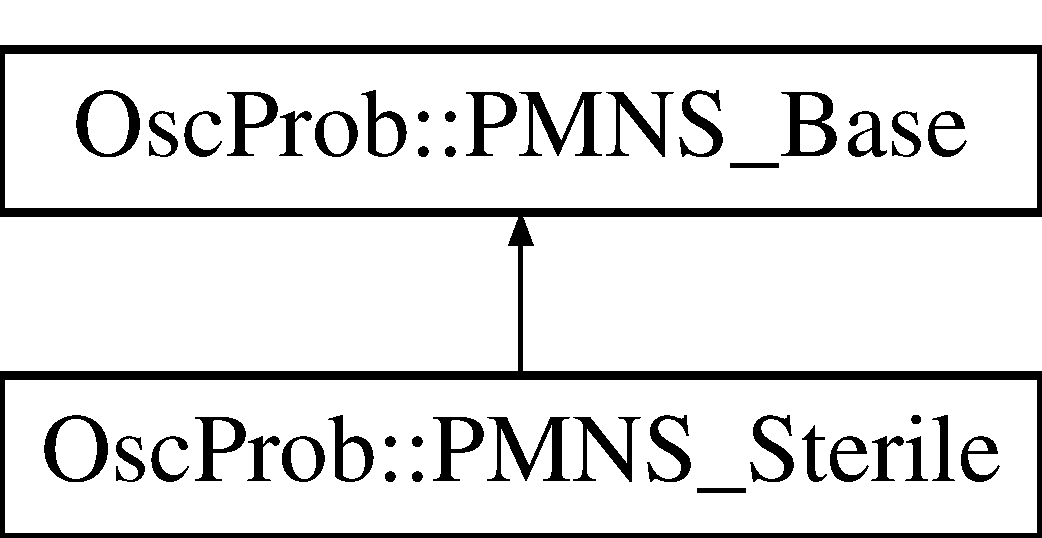
\includegraphics[height=2.000000cm]{classOscProb_1_1PMNS__Sterile}
\end{center}
\end{figure}
\subsection*{Public Types}
\begin{DoxyCompactItemize}
\item 
typedef std\+::complex$<$ double $>$ \hyperlink{classOscProb_1_1PMNS__Base_ae86ec4718808ce9d02e5f5b4226714ab}{complex}
\end{DoxyCompactItemize}
\subsection*{Public Member Functions}
\begin{DoxyCompactItemize}
\item 
\hyperlink{classOscProb_1_1PMNS__Sterile_a774766ab4278d9369a295ffa8e2d272c}{P\+M\+N\+S\+\_\+\+Sterile} (int Num\+Nus)
\begin{DoxyCompactList}\small\item\em Constructor. \end{DoxyCompactList}\item 
virtual \hyperlink{classOscProb_1_1PMNS__Sterile_a992eaf747da2c16f680060d48284c2b9}{$\sim$\+P\+M\+N\+S\+\_\+\+Sterile} ()
\begin{DoxyCompactList}\small\item\em Destructor. \end{DoxyCompactList}\item 
virtual double \hyperlink{classOscProb_1_1PMNS__Base_aec5c399b93261f1962a4b7dbbb44b973}{Prob} (int flvi, int flvf)
\begin{DoxyCompactList}\small\item\em Compute the probability of flvi going to flvf. \end{DoxyCompactList}\item 
virtual double \hyperlink{classOscProb_1_1PMNS__Base_aa3cee10639d5c0879ccb9e78d62128d3}{Prob} (int flvi, int flvf, double E)
\begin{DoxyCompactList}\small\item\em Compute the probability of flvi going to flvf for energy E. \end{DoxyCompactList}\item 
virtual double \hyperlink{classOscProb_1_1PMNS__Base_a6e0a74508d9d6db7be02e242b8467563}{Prob} (int flvi, int flvf, double E, double L)
\begin{DoxyCompactList}\small\item\em Compute the probability of flvi going to flvf for energy E and distance L. \end{DoxyCompactList}\item 
virtual double \hyperlink{classOscProb_1_1PMNS__Base_ac03f754160422e6600da8dbae0f803ed}{Avg\+Prob} (int flvi, int flvf, double E, double dE=0)
\begin{DoxyCompactList}\small\item\em Compute the average probability over a bin of energy. \end{DoxyCompactList}\item 
virtual double \hyperlink{classOscProb_1_1PMNS__Base_ac19a92f4ef428a7333ca8eed76fca637}{Avg\+Prob\+LoE} (int flvi, int flvf, double LoE, double d\+LoE=0)
\begin{DoxyCompactList}\small\item\em Compute the average probability over a bin of L/E. \end{DoxyCompactList}\item 
virtual void \hyperlink{classOscProb_1_1PMNS__Base_ace7875cf6d3bec161a2b7ed2690aec34}{Set\+Angle} (int i, int j, double th)
\begin{DoxyCompactList}\small\item\em Set the mixing angle theta\+\_\+ij. \end{DoxyCompactList}\item 
virtual void \hyperlink{classOscProb_1_1PMNS__Base_a4bef78cfcfc4e70b4ce79cdb8862c0a3}{Set\+Delta} (int i, int j, double delta)
\begin{DoxyCompactList}\small\item\em Set the CP phase delta\+\_\+ij. \end{DoxyCompactList}\item 
virtual void \hyperlink{classOscProb_1_1PMNS__Base_a492243b22fb1b783cd2943f507cff970}{Set\+Dm} (int j, double dm)
\begin{DoxyCompactList}\small\item\em Set the mass-\/splitting dm\+\_\+j1 in e\+V$^\wedge$2. \end{DoxyCompactList}\item 
virtual double \hyperlink{classOscProb_1_1PMNS__Base_acee137091304c919642293ddf015bbc8}{Get\+Angle} (int i, int j)
\begin{DoxyCompactList}\small\item\em Get the mixing angle theta\+\_\+ij. \end{DoxyCompactList}\item 
virtual double \hyperlink{classOscProb_1_1PMNS__Base_adb8dbc91d4286d2e7c8f768c59476241}{Get\+Delta} (int i, int j)
\begin{DoxyCompactList}\small\item\em Get the CP phase delta\+\_\+ij. \end{DoxyCompactList}\item 
virtual double \hyperlink{classOscProb_1_1PMNS__Base_ad26815ac5f4805d1259817e4936e5f8f}{Get\+Dm} (int j)
\begin{DoxyCompactList}\small\item\em Get the mass-\/splitting dm\+\_\+j1 in e\+V$^\wedge$2. \end{DoxyCompactList}\item 
virtual void \hyperlink{classOscProb_1_1PMNS__Base_a4de96ac9b6d1e9b029ab877e57d211ad}{Set\+Std\+Pars} ()
\begin{DoxyCompactList}\small\item\em Set P\+DG 3-\/flavor parameters. \end{DoxyCompactList}\item 
virtual void \hyperlink{classOscProb_1_1PMNS__Base_a95b3b0d0cab5e6a54b5ef99587f837c0}{Set\+Energy} (double E)
\begin{DoxyCompactList}\small\item\em Set the neutrino energy in GeV. \end{DoxyCompactList}\item 
virtual void \hyperlink{classOscProb_1_1PMNS__Base_a717e0348cf762f3961854e332a9b52e0}{Set\+Is\+Nu\+Bar} (bool is\+Nu\+Bar)
\begin{DoxyCompactList}\small\item\em Set the anti-\/neutrino flag. \end{DoxyCompactList}\item 
virtual double \hyperlink{classOscProb_1_1PMNS__Base_acc0d46cc4b8f911b40b807225003bbed}{Get\+Energy} ()
\begin{DoxyCompactList}\small\item\em Get the neutrino energy in GeV. \end{DoxyCompactList}\item 
virtual bool \hyperlink{classOscProb_1_1PMNS__Base_a2f7f2a028dfe7a90fff6b4f757972c2c}{Get\+Is\+Nu\+Bar} ()
\begin{DoxyCompactList}\small\item\em Get the anti-\/neutrino flag. \end{DoxyCompactList}\item 
virtual void \hyperlink{classOscProb_1_1PMNS__Base_ac3b644fd0a56347d304ceca4ae9d8875}{Set\+Path} (\hyperlink{structOscProb_1_1NuPath}{Osc\+Prob\+::\+Nu\+Path} p)
\begin{DoxyCompactList}\small\item\em Set a single path. \end{DoxyCompactList}\item 
virtual void \hyperlink{classOscProb_1_1PMNS__Base_a35b983270613072a3df58b574d80dbfd}{Set\+Path} (double length, double density, double zoa=0.\+5, int layer=0)
\begin{DoxyCompactList}\small\item\em Set a single path. \end{DoxyCompactList}\item 
virtual void \hyperlink{classOscProb_1_1PMNS__Base_a637d19dd850b4246507796526622643c}{Set\+Path} (std\+::vector$<$ \hyperlink{structOscProb_1_1NuPath}{Osc\+Prob\+::\+Nu\+Path} $>$ paths)
\begin{DoxyCompactList}\small\item\em Set a path sequence. \end{DoxyCompactList}\item 
virtual void \hyperlink{classOscProb_1_1PMNS__Base_a887dc9d4dc569ec0cdef3933b4c60efc}{Add\+Path} (\hyperlink{structOscProb_1_1NuPath}{Osc\+Prob\+::\+Nu\+Path} p)
\begin{DoxyCompactList}\small\item\em Add a path to the sequence. \end{DoxyCompactList}\item 
virtual void \hyperlink{classOscProb_1_1PMNS__Base_ab7f89ad9e7e1224adaa59d3c41594cd9}{Add\+Path} (double length, double density, double zoa=0.\+5, int layer=0)
\begin{DoxyCompactList}\small\item\em Add a path to the sequence. \end{DoxyCompactList}\item 
virtual void \hyperlink{classOscProb_1_1PMNS__Base_aefe521239031c418cfaaaa550a6e13bb}{Clear\+Path} ()
\begin{DoxyCompactList}\small\item\em Clear the path vector. \end{DoxyCompactList}\item 
virtual void \hyperlink{classOscProb_1_1PMNS__Base_a6241325b1bd28cafa556daaecbe4ed62}{Set\+Length} (double L)
\begin{DoxyCompactList}\small\item\em Set a single path lentgh in km. \end{DoxyCompactList}\item 
virtual void \hyperlink{classOscProb_1_1PMNS__Base_aa34a40a3b5abda0f252982d9ead3b520}{Set\+Length} (std\+::vector$<$ double $>$ L)
\begin{DoxyCompactList}\small\item\em Set multiple path lengths. \end{DoxyCompactList}\item 
virtual void \hyperlink{classOscProb_1_1PMNS__Base_ac74206f349687da141392c81e2ba6b0d}{Set\+Density} (double rho)
\begin{DoxyCompactList}\small\item\em Set single path density in g/cm$^\wedge$3. \end{DoxyCompactList}\item 
virtual void \hyperlink{classOscProb_1_1PMNS__Base_a858221d5510fe732dc6a101fd305cda0}{Set\+Density} (std\+::vector$<$ double $>$ rho)
\begin{DoxyCompactList}\small\item\em Set multiple path densities. \end{DoxyCompactList}\item 
virtual void \hyperlink{classOscProb_1_1PMNS__Base_a1bf3ea8fd2507fd2fd82d7410ff8f578}{Set\+ZoA} (double zoa)
\begin{DoxyCompactList}\small\item\em Set Z/A value for single path. \end{DoxyCompactList}\item 
virtual void \hyperlink{classOscProb_1_1PMNS__Base_a8495f8a320e1a21965e6a64aec92ad2a}{Set\+ZoA} (std\+::vector$<$ double $>$ zoa)
\begin{DoxyCompactList}\small\item\em Set multiple path Z/A values. \end{DoxyCompactList}\item 
virtual void \hyperlink{classOscProb_1_1PMNS__Base_a904e580edf89fb98bf9a6397739b4ebe}{Set\+Layers} (std\+::vector$<$ int $>$ lay)
\begin{DoxyCompactList}\small\item\em Set multiple path layer indices. \end{DoxyCompactList}\item 
virtual void \hyperlink{classOscProb_1_1PMNS__Base_add6533a9fc9acdfc7ae258b62570d78d}{Set\+Std\+Path} ()
\begin{DoxyCompactList}\small\item\em Set standard neutrino path. \end{DoxyCompactList}\item 
virtual std\+::vector$<$ \hyperlink{structOscProb_1_1NuPath}{Osc\+Prob\+::\+Nu\+Path} $>$ \hyperlink{classOscProb_1_1PMNS__Base_ac8e196f2e85a2b1caaf705073ee95a5c}{Get\+Path} ()
\begin{DoxyCompactList}\small\item\em Get the neutrino path sequence. \end{DoxyCompactList}\item 
virtual std\+::vector$<$ double $>$ \hyperlink{classOscProb_1_1PMNS__Base_a9eac8d768c1424755ee41f7e783af179}{Get\+Sample\+Points} (double LoE, double d\+LoE)
\begin{DoxyCompactList}\small\item\em Compute the sample points for a bin of L/E with width d\+LoE. \end{DoxyCompactList}\end{DoxyCompactItemize}
\subsection*{Protected Member Functions}
\begin{DoxyCompactItemize}
\item 
virtual void \hyperlink{classOscProb_1_1PMNS__Sterile_af60f89862d0fe333c62d6f87ecfd89f8}{Solve\+Ham} ()
\begin{DoxyCompactList}\small\item\em Solve the full Hamiltonian for eigenvectors and eigenvalues. \end{DoxyCompactList}\item 
virtual void \hyperlink{classOscProb_1_1PMNS__Base_adf23b569112f9f9e0e592f01d79a5f3d}{Initialize\+Vectors} ()
\begin{DoxyCompactList}\small\item\em Initialize all member vectors with zeros. \end{DoxyCompactList}\item 
virtual void \hyperlink{classOscProb_1_1PMNS__Base_a986e6ebef09a7e2eb7fee16a4c2c834d}{Set\+Cur\+Path} (\hyperlink{structOscProb_1_1NuPath}{Osc\+Prob\+::\+Nu\+Path} p)
\begin{DoxyCompactList}\small\item\em Set the path currently in use by the class. \end{DoxyCompactList}\item 
virtual void \hyperlink{classOscProb_1_1PMNS__Base_aba565962a440d14bee7a2a96d2eca2c5}{Set\+Att} (double att, int idx)
\begin{DoxyCompactList}\small\item\em Set one of the path attributes. \end{DoxyCompactList}\item 
virtual void \hyperlink{classOscProb_1_1PMNS__Base_aa001479b5f5828c3d16ed087f96ecbcc}{Set\+Att} (std\+::vector$<$ double $>$ att, int idx)
\begin{DoxyCompactList}\small\item\em Set all values of a path attribute. \end{DoxyCompactList}\item 
virtual void \hyperlink{classOscProb_1_1PMNS__Base_aae18afd69074211335f49ec40e6011b9}{RotateH} (int i, int j)
\begin{DoxyCompactList}\small\item\em Rotate the Hamiltonian by theta\+\_\+ij and delta\+\_\+ij. \end{DoxyCompactList}\item 
virtual void \hyperlink{classOscProb_1_1PMNS__Base_ad0faf5eae755afb1baa1fcd5ffebad41}{Build\+Hms} ()
\begin{DoxyCompactList}\small\item\em Build the matrix of masses squared. \end{DoxyCompactList}\item 
virtual void \hyperlink{classOscProb_1_1PMNS__Base_ac0d4bf8ff1318ef96d3dafa62e0cec25}{Reset\+To\+Flavour} (int flv)
\begin{DoxyCompactList}\small\item\em Reset neutrino state to pure flavour flv. \end{DoxyCompactList}\item 
virtual void \hyperlink{classOscProb_1_1PMNS__Base_accb08503acc162188041d7a96a280462}{Propagate\+Path} (\hyperlink{structOscProb_1_1NuPath}{Osc\+Prob\+::\+Nu\+Path} p)
\begin{DoxyCompactList}\small\item\em Propagate neutrino through a single path. \end{DoxyCompactList}\item 
virtual void \hyperlink{classOscProb_1_1PMNS__Base_a054e3a8b05b9a958b6fa416e4a835e3e}{Propagate} ()
\begin{DoxyCompactList}\small\item\em Propagate neutrino through full path. \end{DoxyCompactList}\item 
virtual double \hyperlink{classOscProb_1_1PMNS__Base_a0dc4d45bc3d7e03b9abbf5b4e100cc22}{P} (int flv)
\begin{DoxyCompactList}\small\item\em Return the probability of final state in flavour flv. \end{DoxyCompactList}\end{DoxyCompactItemize}
\subsection*{Protected Attributes}
\begin{DoxyCompactItemize}
\item 
gsl\+\_\+vector $\ast$ \hyperlink{classOscProb_1_1PMNS__Sterile_abdcb0a144aadef0239dfb36ed4ed0297}{f\+Eval\+G\+SL}
\begin{DoxyCompactList}\small\item\em Stores the G\+SL eigenvalues. \end{DoxyCompactList}\item 
gsl\+\_\+matrix\+\_\+complex $\ast$ \hyperlink{classOscProb_1_1PMNS__Sterile_a8ab71bc7de328eb6ba855904f365fb1d}{f\+Evec\+G\+SL}
\begin{DoxyCompactList}\small\item\em Stores the G\+SL eigenvectors. \end{DoxyCompactList}\item 
gsl\+\_\+matrix\+\_\+complex $\ast$ \hyperlink{classOscProb_1_1PMNS__Sterile_aeff790051925a3135b7529ced67e81ab}{H\+\_\+\+G\+SL}
\begin{DoxyCompactList}\small\item\em The Hamiltonian to be solved by G\+SL. \end{DoxyCompactList}\item 
gsl\+\_\+eigen\+\_\+hermv\+\_\+workspace $\ast$ \hyperlink{classOscProb_1_1PMNS__Sterile_a4e8aed8fd29297e4833488572c9a4eb1}{W\+\_\+\+G\+SL}
\begin{DoxyCompactList}\small\item\em Allocates memory for G\+SL solution. \end{DoxyCompactList}\item 
int \hyperlink{classOscProb_1_1PMNS__Base_a24bb74bed63569dfe88b18fa6a08060e}{f\+Num\+Nus}
\begin{DoxyCompactList}\small\item\em Number of neutrino flavours. \end{DoxyCompactList}\item 
std\+::vector$<$ double $>$ \hyperlink{classOscProb_1_1PMNS__Base_a406a31c3b5d620e5a0cace5b411f9f70}{f\+Dm}
\begin{DoxyCompactList}\small\item\em m$^\wedge$2\+\_\+i -\/ m$^\wedge$2\+\_\+1 in vacuum \end{DoxyCompactList}\item 
std\+::vector$<$ std\+::vector$<$ double $>$ $>$ \hyperlink{classOscProb_1_1PMNS__Base_a1976887cd658dd86b2336c181f1470b4}{f\+Theta}
\begin{DoxyCompactList}\small\item\em theta\mbox{[}i\mbox{]}\mbox{[}j\mbox{]} mixing angle \end{DoxyCompactList}\item 
std\+::vector$<$ std\+::vector$<$ double $>$ $>$ \hyperlink{classOscProb_1_1PMNS__Base_ab2a5fa40e689b221c8a7d2c17213810d}{f\+Delta}
\begin{DoxyCompactList}\small\item\em delta\mbox{[}i\mbox{]}\mbox{[}j\mbox{]} CP violating phase \end{DoxyCompactList}\item 
std\+::vector$<$ \hyperlink{classOscProb_1_1PMNS__Base_ae86ec4718808ce9d02e5f5b4226714ab}{complex} $>$ \hyperlink{classOscProb_1_1PMNS__Base_ad38a7107c3ab393591fd5ba21658300b}{f\+Nu\+State}
\begin{DoxyCompactList}\small\item\em The neutrino current state. \end{DoxyCompactList}\item 
std\+::vector$<$ std\+::vector$<$ \hyperlink{classOscProb_1_1PMNS__Base_ae86ec4718808ce9d02e5f5b4226714ab}{complex} $>$ $>$ \hyperlink{classOscProb_1_1PMNS__Base_adf5901166216e8c7a5cff2092952f473}{f\+Hms}
\begin{DoxyCompactList}\small\item\em matrix H$\ast$2E in e\+V$^\wedge$2 \end{DoxyCompactList}\item 
std\+::vector$<$ double $>$ \hyperlink{classOscProb_1_1PMNS__Base_a6319c34d7decbb9d7d6da279c06e8c2d}{f\+Eval}
\begin{DoxyCompactList}\small\item\em Eigenvalues of the Hamiltonian. \end{DoxyCompactList}\item 
std\+::vector$<$ std\+::vector$<$ \hyperlink{classOscProb_1_1PMNS__Base_ae86ec4718808ce9d02e5f5b4226714ab}{complex} $>$ $>$ \hyperlink{classOscProb_1_1PMNS__Base_a093e7bd31d4ef52ed52df414e12c1d17}{f\+Evec}
\begin{DoxyCompactList}\small\item\em Eigenvectors of the Hamiltonian. \end{DoxyCompactList}\item 
double \hyperlink{classOscProb_1_1PMNS__Base_a2800af6d436972f3e900867790c046b0}{f\+Energy}
\begin{DoxyCompactList}\small\item\em Neutrino energy. \end{DoxyCompactList}\item 
bool \hyperlink{classOscProb_1_1PMNS__Base_a0ebaeaefab36a3ff381c6293faedfdd6}{f\+Is\+Nu\+Bar}
\begin{DoxyCompactList}\small\item\em Anti-\/neutrino flag. \end{DoxyCompactList}\item 
std\+::vector$<$ \hyperlink{structOscProb_1_1NuPath}{Osc\+Prob\+::\+Nu\+Path} $>$ \hyperlink{classOscProb_1_1PMNS__Base_a69db9d57e12fc7cbe0431bc6c18fac93}{f\+Nu\+Paths}
\begin{DoxyCompactList}\small\item\em Vector of neutrino paths. \end{DoxyCompactList}\item 
\hyperlink{structOscProb_1_1NuPath}{Osc\+Prob\+::\+Nu\+Path} \hyperlink{classOscProb_1_1PMNS__Base_a849437aa8891fe042e86886ce8f81c6e}{f\+Path}
\begin{DoxyCompactList}\small\item\em Current neutrino path. \end{DoxyCompactList}\item 
bool \hyperlink{classOscProb_1_1PMNS__Base_a9ac3cadeac8db1b90f3152f476244780}{f\+Built\+Hms}
\begin{DoxyCompactList}\small\item\em Tag to avoid rebuilding Hms. \end{DoxyCompactList}\item 
bool \hyperlink{classOscProb_1_1PMNS__Base_a6dc5cd010d2d70b2324745b4e53e9839}{f\+Got\+ES}
\begin{DoxyCompactList}\small\item\em Tag to avoid recalculating eigensystem. \end{DoxyCompactList}\end{DoxyCompactItemize}
\subsection*{Static Protected Attributes}
\begin{DoxyCompactItemize}
\item 
static const \hyperlink{classOscProb_1_1PMNS__Base_ae86ec4718808ce9d02e5f5b4226714ab}{complex} \hyperlink{classOscProb_1_1PMNS__Base_a5c31ed4593cf95feb36fb80c1850d25e}{zero}
\begin{DoxyCompactList}\small\item\em zero in complex \end{DoxyCompactList}\item 
static const \hyperlink{classOscProb_1_1PMNS__Base_ae86ec4718808ce9d02e5f5b4226714ab}{complex} \hyperlink{classOscProb_1_1PMNS__Base_ab64aab27448a5aca27565c991a9d173e}{one}
\begin{DoxyCompactList}\small\item\em one in complex \end{DoxyCompactList}\item 
static const double \hyperlink{classOscProb_1_1PMNS__Base_a382ddd7b76ca89b43f22614a2ea7327b}{k\+Km2eV} = 1.\+0 / 1.\+973269718e-\/10
\begin{DoxyCompactList}\small\item\em km to e\+V$^\wedge$-\/1 \end{DoxyCompactList}\item 
static const double \hyperlink{classOscProb_1_1PMNS__Base_a326fc5016d7dd7ce05682c06cdcb6d94}{k\+K2} = 4.\+62711501e-\/09
\begin{DoxyCompactList}\small\item\em mol/\+Ge\+V$^\wedge$2/cm$^\wedge$3 to eV \end{DoxyCompactList}\item 
static const double \hyperlink{classOscProb_1_1PMNS__Base_ad36a0a6bf58d6ec093d3947784bd89e9}{k\+Ge\+V2eV} = 1.\+0e+09
\begin{DoxyCompactList}\small\item\em GeV to eV. \end{DoxyCompactList}\item 
static const double \hyperlink{classOscProb_1_1PMNS__Base_a7f26a3456128234b2ae6cc9141a6532f}{k\+Gf} = 1.\+1663787e-\/05
\begin{DoxyCompactList}\small\item\em G\+\_\+F in units of Ge\+V$^\wedge$-\/2. \end{DoxyCompactList}\end{DoxyCompactItemize}


\subsection{Detailed Description}
This class implements neutrino oscillations for any number of neutrino falvours. The extra flavours above 3 are treated as sterile neutrinos, i.\+e. it implements a 3+N model. One can also run a 2-\/neutrino model in principle, but an analytical solution would be feasible and more efficient in that case.

The eigensystem solution is performed by G\+SL, which makes it slower than the \hyperlink{classOscProb_1_1PMNS__Fast}{P\+M\+N\+S\+\_\+\+Fast} class, which only works for 3 neutrinos.

\begin{DoxyAuthor}{Author}
jcoelho@apc.\+in2p3.\+fr 
\end{DoxyAuthor}


Definition at line 26 of file P\+M\+N\+S\+\_\+\+Sterile.\+h.



\subsection{Member Typedef Documentation}
\index{Osc\+Prob\+::\+P\+M\+N\+S\+\_\+\+Sterile@{Osc\+Prob\+::\+P\+M\+N\+S\+\_\+\+Sterile}!complex@{complex}}
\index{complex@{complex}!Osc\+Prob\+::\+P\+M\+N\+S\+\_\+\+Sterile@{Osc\+Prob\+::\+P\+M\+N\+S\+\_\+\+Sterile}}
\subsubsection[{\texorpdfstring{complex}{complex}}]{\setlength{\rightskip}{0pt plus 5cm}typedef std\+::complex$<$double$>$ {\bf Osc\+Prob\+::\+P\+M\+N\+S\+\_\+\+Base\+::complex}\hspace{0.3cm}{\ttfamily [inherited]}}\hypertarget{classOscProb_1_1PMNS__Base_ae86ec4718808ce9d02e5f5b4226714ab}{}\label{classOscProb_1_1PMNS__Base_ae86ec4718808ce9d02e5f5b4226714ab}


Definition at line 105 of file P\+M\+N\+S\+\_\+\+Base.\+h.



\subsection{Constructor \& Destructor Documentation}
\index{Osc\+Prob\+::\+P\+M\+N\+S\+\_\+\+Sterile@{Osc\+Prob\+::\+P\+M\+N\+S\+\_\+\+Sterile}!P\+M\+N\+S\+\_\+\+Sterile@{P\+M\+N\+S\+\_\+\+Sterile}}
\index{P\+M\+N\+S\+\_\+\+Sterile@{P\+M\+N\+S\+\_\+\+Sterile}!Osc\+Prob\+::\+P\+M\+N\+S\+\_\+\+Sterile@{Osc\+Prob\+::\+P\+M\+N\+S\+\_\+\+Sterile}}
\subsubsection[{\texorpdfstring{P\+M\+N\+S\+\_\+\+Sterile(int Num\+Nus)}{PMNS_Sterile(int NumNus)}}]{\setlength{\rightskip}{0pt plus 5cm}P\+M\+N\+S\+\_\+\+Sterile\+::\+P\+M\+N\+S\+\_\+\+Sterile (
\begin{DoxyParamCaption}
\item[{int}]{num\+Nus}
\end{DoxyParamCaption}
)}\hypertarget{classOscProb_1_1PMNS__Sterile_a774766ab4278d9369a295ffa8e2d272c}{}\label{classOscProb_1_1PMNS__Sterile_a774766ab4278d9369a295ffa8e2d272c}
Constructor. \begin{DoxySeeAlso}{See also}
\hyperlink{classOscProb_1_1PMNS__Base_aa53e83b03a9cf4bdfa0a07136bd17a79}{P\+M\+N\+S\+\_\+\+Base\+::\+P\+M\+N\+S\+\_\+\+Base}
\end{DoxySeeAlso}
This class can implement any number of neutrino flavours.


\begin{DoxyParams}{Parameters}
{\em num\+Nus} & -\/ the number of neutrino flavours \\
\hline
\end{DoxyParams}


Definition at line 38 of file P\+M\+N\+S\+\_\+\+Sterile.\+cxx.



References f\+Eval\+G\+SL, f\+Evec\+G\+SL, Osc\+Prob\+::\+P\+M\+N\+S\+\_\+\+Base\+::f\+Num\+Nus, H\+\_\+\+G\+SL, and W\+\_\+\+G\+SL.


\begin{DoxyCode}
38                                      : \hyperlink{classOscProb_1_1PMNS__Base_aa53e83b03a9cf4bdfa0a07136bd17a79}{PMNS\_Base}(numNus),
39 \hyperlink{classOscProb_1_1PMNS__Sterile_abdcb0a144aadef0239dfb36ed4ed0297}{fEvalGSL}(0), \hyperlink{classOscProb_1_1PMNS__Sterile_a8ab71bc7de328eb6ba855904f365fb1d}{fEvecGSL}(0), \hyperlink{classOscProb_1_1PMNS__Sterile_aeff790051925a3135b7529ced67e81ab}{H\_GSL}(0), \hyperlink{classOscProb_1_1PMNS__Sterile_a4e8aed8fd29297e4833488572c9a4eb1}{W\_GSL}(0)
40 \{
41 
42   \textcolor{comment}{// Allocate memory for the GSL objects}
43   \hyperlink{classOscProb_1_1PMNS__Sterile_abdcb0a144aadef0239dfb36ed4ed0297}{fEvalGSL} = gsl\_vector\_alloc(\hyperlink{classOscProb_1_1PMNS__Base_a24bb74bed63569dfe88b18fa6a08060e}{fNumNus});
44   \hyperlink{classOscProb_1_1PMNS__Sterile_a8ab71bc7de328eb6ba855904f365fb1d}{fEvecGSL} = gsl\_matrix\_complex\_alloc(\hyperlink{classOscProb_1_1PMNS__Base_a24bb74bed63569dfe88b18fa6a08060e}{fNumNus}, \hyperlink{classOscProb_1_1PMNS__Base_a24bb74bed63569dfe88b18fa6a08060e}{fNumNus});
45   \hyperlink{classOscProb_1_1PMNS__Sterile_aeff790051925a3135b7529ced67e81ab}{H\_GSL} = gsl\_matrix\_complex\_alloc(\hyperlink{classOscProb_1_1PMNS__Base_a24bb74bed63569dfe88b18fa6a08060e}{fNumNus}, \hyperlink{classOscProb_1_1PMNS__Base_a24bb74bed63569dfe88b18fa6a08060e}{fNumNus});
46   \hyperlink{classOscProb_1_1PMNS__Sterile_a4e8aed8fd29297e4833488572c9a4eb1}{W\_GSL} = gsl\_eigen\_hermv\_alloc(\hyperlink{classOscProb_1_1PMNS__Base_a24bb74bed63569dfe88b18fa6a08060e}{fNumNus});
47 
48 \}
\end{DoxyCode}
\index{Osc\+Prob\+::\+P\+M\+N\+S\+\_\+\+Sterile@{Osc\+Prob\+::\+P\+M\+N\+S\+\_\+\+Sterile}!````~P\+M\+N\+S\+\_\+\+Sterile@{$\sim$\+P\+M\+N\+S\+\_\+\+Sterile}}
\index{````~P\+M\+N\+S\+\_\+\+Sterile@{$\sim$\+P\+M\+N\+S\+\_\+\+Sterile}!Osc\+Prob\+::\+P\+M\+N\+S\+\_\+\+Sterile@{Osc\+Prob\+::\+P\+M\+N\+S\+\_\+\+Sterile}}
\subsubsection[{\texorpdfstring{$\sim$\+P\+M\+N\+S\+\_\+\+Sterile()}{~PMNS_Sterile()}}]{\setlength{\rightskip}{0pt plus 5cm}P\+M\+N\+S\+\_\+\+Sterile\+::$\sim$\+P\+M\+N\+S\+\_\+\+Sterile (
\begin{DoxyParamCaption}
{}
\end{DoxyParamCaption}
)\hspace{0.3cm}{\ttfamily [virtual]}}\hypertarget{classOscProb_1_1PMNS__Sterile_a992eaf747da2c16f680060d48284c2b9}{}\label{classOscProb_1_1PMNS__Sterile_a992eaf747da2c16f680060d48284c2b9}
Destructor.

Clear G\+SL objects. 

Definition at line 56 of file P\+M\+N\+S\+\_\+\+Sterile.\+cxx.



References f\+Eval\+G\+SL, f\+Evec\+G\+SL, H\+\_\+\+G\+SL, and W\+\_\+\+G\+SL.


\begin{DoxyCode}
56                            \{
57 
58   \textcolor{comment}{// Free memory from GSL objects}
59   gsl\_matrix\_complex\_free(\hyperlink{classOscProb_1_1PMNS__Sterile_aeff790051925a3135b7529ced67e81ab}{H\_GSL}); \hyperlink{classOscProb_1_1PMNS__Sterile_aeff790051925a3135b7529ced67e81ab}{H\_GSL} = 0;
60   gsl\_eigen\_hermv\_free(\hyperlink{classOscProb_1_1PMNS__Sterile_a4e8aed8fd29297e4833488572c9a4eb1}{W\_GSL}); \hyperlink{classOscProb_1_1PMNS__Sterile_a4e8aed8fd29297e4833488572c9a4eb1}{W\_GSL} = 0;
61   gsl\_matrix\_complex\_free(\hyperlink{classOscProb_1_1PMNS__Sterile_a8ab71bc7de328eb6ba855904f365fb1d}{fEvecGSL}); \hyperlink{classOscProb_1_1PMNS__Sterile_a8ab71bc7de328eb6ba855904f365fb1d}{fEvecGSL} = 0;
62   gsl\_vector\_free(\hyperlink{classOscProb_1_1PMNS__Sterile_abdcb0a144aadef0239dfb36ed4ed0297}{fEvalGSL}); \hyperlink{classOscProb_1_1PMNS__Sterile_abdcb0a144aadef0239dfb36ed4ed0297}{fEvalGSL} = 0;
63 
64 \}
\end{DoxyCode}


\subsection{Member Function Documentation}
\index{Osc\+Prob\+::\+P\+M\+N\+S\+\_\+\+Sterile@{Osc\+Prob\+::\+P\+M\+N\+S\+\_\+\+Sterile}!Add\+Path@{Add\+Path}}
\index{Add\+Path@{Add\+Path}!Osc\+Prob\+::\+P\+M\+N\+S\+\_\+\+Sterile@{Osc\+Prob\+::\+P\+M\+N\+S\+\_\+\+Sterile}}
\subsubsection[{\texorpdfstring{Add\+Path(\+Osc\+Prob\+::\+Nu\+Path p)}{AddPath(OscProb::NuPath p)}}]{\setlength{\rightskip}{0pt plus 5cm}void P\+M\+N\+S\+\_\+\+Base\+::\+Add\+Path (
\begin{DoxyParamCaption}
\item[{{\bf Osc\+Prob\+::\+Nu\+Path}}]{p}
\end{DoxyParamCaption}
)\hspace{0.3cm}{\ttfamily [virtual]}, {\ttfamily [inherited]}}\hypertarget{classOscProb_1_1PMNS__Base_a887dc9d4dc569ec0cdef3933b4c60efc}{}\label{classOscProb_1_1PMNS__Base_a887dc9d4dc569ec0cdef3933b4c60efc}
Add a path to the sequence. 
\begin{DoxyParams}{Parameters}
{\em p} & -\/ A neutrino path segment \\
\hline
\end{DoxyParams}


Definition at line 256 of file P\+M\+N\+S\+\_\+\+Base.\+cxx.



References Osc\+Prob\+::\+P\+M\+N\+S\+\_\+\+Base\+::f\+Nu\+Paths.



Referenced by Osc\+Prob\+::\+P\+M\+N\+S\+\_\+\+Base\+::\+Add\+Path(), Osc\+Prob\+::\+P\+M\+N\+S\+\_\+\+Base\+::\+Set\+Att(), and Osc\+Prob\+::\+P\+M\+N\+S\+\_\+\+Base\+::\+Set\+Path().


\begin{DoxyCode}
256                                \{
257 
258   \hyperlink{classOscProb_1_1PMNS__Base_a69db9d57e12fc7cbe0431bc6c18fac93}{fNuPaths}.push\_back(p);
259 
260 \}
\end{DoxyCode}
\index{Osc\+Prob\+::\+P\+M\+N\+S\+\_\+\+Sterile@{Osc\+Prob\+::\+P\+M\+N\+S\+\_\+\+Sterile}!Add\+Path@{Add\+Path}}
\index{Add\+Path@{Add\+Path}!Osc\+Prob\+::\+P\+M\+N\+S\+\_\+\+Sterile@{Osc\+Prob\+::\+P\+M\+N\+S\+\_\+\+Sterile}}
\subsubsection[{\texorpdfstring{Add\+Path(double length, double density, double zoa=0.\+5, int layer=0)}{AddPath(double length, double density, double zoa=0.5, int layer=0)}}]{\setlength{\rightskip}{0pt plus 5cm}void P\+M\+N\+S\+\_\+\+Base\+::\+Add\+Path (
\begin{DoxyParamCaption}
\item[{double}]{length, }
\item[{double}]{density, }
\item[{double}]{zoa = {\ttfamily 0.5}, }
\item[{int}]{layer = {\ttfamily 0}}
\end{DoxyParamCaption}
)\hspace{0.3cm}{\ttfamily [virtual]}, {\ttfamily [inherited]}}\hypertarget{classOscProb_1_1PMNS__Base_ab7f89ad9e7e1224adaa59d3c41594cd9}{}\label{classOscProb_1_1PMNS__Base_ab7f89ad9e7e1224adaa59d3c41594cd9}
Add a path to the sequence defining attributes directly. 
\begin{DoxyParams}{Parameters}
{\em length} & -\/ The length of the path segment in km \\
\hline
{\em density} & -\/ The density of the path segment in g/cm$^\wedge$3 \\
\hline
{\em zoa} & -\/ The effective Z/A of the path segment \\
\hline
{\em layer} & -\/ An index to identify the layer type (e.\+g. earth inner core) \\
\hline
\end{DoxyParams}


Definition at line 270 of file P\+M\+N\+S\+\_\+\+Base.\+cxx.



References Osc\+Prob\+::\+P\+M\+N\+S\+\_\+\+Base\+::\+Add\+Path().


\begin{DoxyCode}
270                                                                            \{
271 
272   \hyperlink{classOscProb_1_1PMNS__Base_a887dc9d4dc569ec0cdef3933b4c60efc}{AddPath}(\hyperlink{structOscProb_1_1NuPath}{NuPath}(length, density, zoa, layer));
273 
274 \}
\end{DoxyCode}
\index{Osc\+Prob\+::\+P\+M\+N\+S\+\_\+\+Sterile@{Osc\+Prob\+::\+P\+M\+N\+S\+\_\+\+Sterile}!Avg\+Prob@{Avg\+Prob}}
\index{Avg\+Prob@{Avg\+Prob}!Osc\+Prob\+::\+P\+M\+N\+S\+\_\+\+Sterile@{Osc\+Prob\+::\+P\+M\+N\+S\+\_\+\+Sterile}}
\subsubsection[{\texorpdfstring{Avg\+Prob(int flvi, int flvf, double E, double d\+E=0)}{AvgProb(int flvi, int flvf, double E, double dE=0)}}]{\setlength{\rightskip}{0pt plus 5cm}double P\+M\+N\+S\+\_\+\+Base\+::\+Avg\+Prob (
\begin{DoxyParamCaption}
\item[{int}]{flvi, }
\item[{int}]{flvf, }
\item[{double}]{E, }
\item[{double}]{dE = {\ttfamily 0}}
\end{DoxyParamCaption}
)\hspace{0.3cm}{\ttfamily [virtual]}, {\ttfamily [inherited]}}\hypertarget{classOscProb_1_1PMNS__Base_ac03f754160422e6600da8dbae0f803ed}{}\label{classOscProb_1_1PMNS__Base_ac03f754160422e6600da8dbae0f803ed}
Compute the average probability of flvi going to flvf over a bin of energy E with width dE.

This gets transformed into L/E, since the oscillation terms have arguments linear in L/E and not E.

This function currently only works for single paths.

Flavours are\+: 
\begin{DoxyPre}
  0 = nue, 1 = numu, 2 = nutau
  3 = sterile\_1, 4 = sterile\_2, etc.
\end{DoxyPre}
 
\begin{DoxyParams}{Parameters}
{\em flvi} & -\/ The neutrino starting flavour. \\
\hline
{\em flvf} & -\/ The neutrino final flavour. \\
\hline
{\em E} & -\/ The neutrino energy in the bin center in GeV \\
\hline
{\em dE} & -\/ The energy bin width in GeV\\
\hline
\end{DoxyParams}
\begin{DoxyReturn}{Returns}
Average neutrino oscillation probability 
\end{DoxyReturn}


Definition at line 1076 of file P\+M\+N\+S\+\_\+\+Base.\+cxx.



References Osc\+Prob\+::\+P\+M\+N\+S\+\_\+\+Base\+::\+Avg\+Prob\+Lo\+E(), Osc\+Prob\+::\+P\+M\+N\+S\+\_\+\+Base\+::f\+Nu\+Paths, Osc\+Prob\+::\+P\+M\+N\+S\+\_\+\+Base\+::f\+Path, Osc\+Prob\+::\+Nu\+Path\+::length, Osc\+Prob\+::\+P\+M\+N\+S\+\_\+\+Base\+::\+Prob(), and Osc\+Prob\+::\+P\+M\+N\+S\+\_\+\+Base\+::\+Set\+Cur\+Path().


\begin{DoxyCode}
1077 \{
1078 
1079   \textcolor{comment}{// Do nothing if energy is not positive}
1080   \textcolor{keywordflow}{if}(E<=0) \textcolor{keywordflow}{return} 0;
1081 
1082   \textcolor{keywordflow}{if}(\hyperlink{classOscProb_1_1PMNS__Base_a69db9d57e12fc7cbe0431bc6c18fac93}{fNuPaths}.empty()) \textcolor{keywordflow}{return} 0;
1083 
1084   \textcolor{keywordflow}{if}(\hyperlink{classOscProb_1_1PMNS__Base_a69db9d57e12fc7cbe0431bc6c18fac93}{fNuPaths}.size() != 1)\{
1085     cout << \textcolor{stringliteral}{"ERROR: AvgProb not implemented for multiple paths."} << endl;
1086     cout << \textcolor{stringliteral}{"       Returning probability at bin center."} << endl;
1087     \textcolor{keywordflow}{return} \hyperlink{classOscProb_1_1PMNS__Base_aec5c399b93261f1962a4b7dbbb44b973}{Prob}(flvi, flvf, E);
1088   \}
1089 
1090   \textcolor{comment}{// Don't average zero width}
1091   \textcolor{keywordflow}{if}(dE<=0) \textcolor{keywordflow}{return} \hyperlink{classOscProb_1_1PMNS__Base_aec5c399b93261f1962a4b7dbbb44b973}{Prob}(flvi, flvf, E);
1092 
1093   \textcolor{comment}{// Make sure fPath is set}
1094   \hyperlink{classOscProb_1_1PMNS__Base_a986e6ebef09a7e2eb7fee16a4c2c834d}{SetCurPath}(\hyperlink{classOscProb_1_1PMNS__Base_a69db9d57e12fc7cbe0431bc6c18fac93}{fNuPaths}[0]);
1095 
1096   \textcolor{comment}{// Define L/E variables}
1097   \textcolor{keywordtype}{double} LoE = 0;
1098   \textcolor{keywordtype}{double} dLoE = 0;
1099 
1100   \textcolor{comment}{// Set a minimum energy}
1101   \textcolor{keywordtype}{double} minE = 0.1 * E;
1102 
1103   \textcolor{comment}{// Transform range to L/E}
1104   \textcolor{comment}{// Full range if low edge > minE}
1105   \textcolor{keywordflow}{if}(E-dE/2 > minE)\{
1106     LoE = 0.5 * (\hyperlink{classOscProb_1_1PMNS__Base_a849437aa8891fe042e86886ce8f81c6e}{fPath}.\hyperlink{structOscProb_1_1NuPath_af22660894b6e25cf835500381b155557}{length}/(E-dE/2) + \hyperlink{classOscProb_1_1PMNS__Base_a849437aa8891fe042e86886ce8f81c6e}{fPath}.\hyperlink{structOscProb_1_1NuPath_af22660894b6e25cf835500381b155557}{length}/(E+dE/2));
1107     dLoE = \hyperlink{classOscProb_1_1PMNS__Base_a849437aa8891fe042e86886ce8f81c6e}{fPath}.\hyperlink{structOscProb_1_1NuPath_af22660894b6e25cf835500381b155557}{length}/(E-dE/2) - \hyperlink{classOscProb_1_1PMNS__Base_a849437aa8891fe042e86886ce8f81c6e}{fPath}.\hyperlink{structOscProb_1_1NuPath_af22660894b6e25cf835500381b155557}{length}/(E+dE/2);
1108   \}
1109   \textcolor{comment}{// Else start at minE}
1110   \textcolor{keywordflow}{else}\{
1111     LoE = 0.5 * (\hyperlink{classOscProb_1_1PMNS__Base_a849437aa8891fe042e86886ce8f81c6e}{fPath}.\hyperlink{structOscProb_1_1NuPath_af22660894b6e25cf835500381b155557}{length}/minE + \hyperlink{classOscProb_1_1PMNS__Base_a849437aa8891fe042e86886ce8f81c6e}{fPath}.\hyperlink{structOscProb_1_1NuPath_af22660894b6e25cf835500381b155557}{length}/(E+dE/2));
1112     dLoE = \hyperlink{classOscProb_1_1PMNS__Base_a849437aa8891fe042e86886ce8f81c6e}{fPath}.\hyperlink{structOscProb_1_1NuPath_af22660894b6e25cf835500381b155557}{length}/minE - \hyperlink{classOscProb_1_1PMNS__Base_a849437aa8891fe042e86886ce8f81c6e}{fPath}.\hyperlink{structOscProb_1_1NuPath_af22660894b6e25cf835500381b155557}{length}/(E+dE/2);
1113   \}
1114 
1115   \textcolor{comment}{// Compute average in LoE}
1116   \textcolor{keywordflow}{return} \hyperlink{classOscProb_1_1PMNS__Base_ac19a92f4ef428a7333ca8eed76fca637}{AvgProbLoE}(flvi, flvf, LoE, dLoE);
1117 
1118 \}
\end{DoxyCode}
\index{Osc\+Prob\+::\+P\+M\+N\+S\+\_\+\+Sterile@{Osc\+Prob\+::\+P\+M\+N\+S\+\_\+\+Sterile}!Avg\+Prob\+LoE@{Avg\+Prob\+LoE}}
\index{Avg\+Prob\+LoE@{Avg\+Prob\+LoE}!Osc\+Prob\+::\+P\+M\+N\+S\+\_\+\+Sterile@{Osc\+Prob\+::\+P\+M\+N\+S\+\_\+\+Sterile}}
\subsubsection[{\texorpdfstring{Avg\+Prob\+Lo\+E(int flvi, int flvf, double Lo\+E, double d\+Lo\+E=0)}{AvgProbLoE(int flvi, int flvf, double LoE, double dLoE=0)}}]{\setlength{\rightskip}{0pt plus 5cm}double P\+M\+N\+S\+\_\+\+Base\+::\+Avg\+Prob\+LoE (
\begin{DoxyParamCaption}
\item[{int}]{flvi, }
\item[{int}]{flvf, }
\item[{double}]{LoE, }
\item[{double}]{d\+LoE = {\ttfamily 0}}
\end{DoxyParamCaption}
)\hspace{0.3cm}{\ttfamily [virtual]}, {\ttfamily [inherited]}}\hypertarget{classOscProb_1_1PMNS__Base_ac19a92f4ef428a7333ca8eed76fca637}{}\label{classOscProb_1_1PMNS__Base_ac19a92f4ef428a7333ca8eed76fca637}
Compute the average probability of flvi going to flvf over a bin of L/E with width d\+LoE.

The probabilities are weighted by (L/E)$^\wedge$-\/2 so that event density is flat in energy. This avoids giving too much weight to low energies. Better approximations would be achieved if we used an interpolated event density.

This function currently only works for single paths.

Flavours are\+: 
\begin{DoxyPre}
  0 = nue, 1 = numu, 2 = nutau
  3 = sterile\_1, 4 = sterile\_2, etc.
\end{DoxyPre}
 
\begin{DoxyParams}{Parameters}
{\em flvi} & -\/ The neutrino starting flavour. \\
\hline
{\em flvf} & -\/ The neutrino final flavour. \\
\hline
{\em LoE} & -\/ The neutrino L/E value in the bin center in km/\+GeV \\
\hline
{\em d\+LoE} & -\/ The L/E bin width in km/\+GeV\\
\hline
\end{DoxyParams}
\begin{DoxyReturn}{Returns}
Average neutrino oscillation probability 
\end{DoxyReturn}


Definition at line 1144 of file P\+M\+N\+S\+\_\+\+Base.\+cxx.



References Osc\+Prob\+::\+P\+M\+N\+S\+\_\+\+Base\+::f\+Nu\+Paths, Osc\+Prob\+::\+P\+M\+N\+S\+\_\+\+Base\+::f\+Path, Osc\+Prob\+::\+P\+M\+N\+S\+\_\+\+Base\+::\+Get\+Sample\+Points(), Osc\+Prob\+::\+Nu\+Path\+::length, Osc\+Prob\+::\+P\+M\+N\+S\+\_\+\+Base\+::\+Prob(), Osc\+Prob\+::\+P\+M\+N\+S\+\_\+\+Base\+::\+Set\+Cur\+Path(), and Osc\+Prob\+::\+P\+M\+N\+S\+\_\+\+Base\+::\+Set\+Energy().



Referenced by Osc\+Prob\+::\+P\+M\+N\+S\+\_\+\+Base\+::\+Avg\+Prob().


\begin{DoxyCode}
1145 \{
1146 
1147   \textcolor{comment}{// Do nothing if L/E is not positive}
1148   \textcolor{keywordflow}{if}(LoE<=0) \textcolor{keywordflow}{return} 0;
1149 
1150   \textcolor{keywordflow}{if}(\hyperlink{classOscProb_1_1PMNS__Base_a69db9d57e12fc7cbe0431bc6c18fac93}{fNuPaths}.empty()) \textcolor{keywordflow}{return} 0;
1151 
1152   \textcolor{keywordflow}{if}(\hyperlink{classOscProb_1_1PMNS__Base_a69db9d57e12fc7cbe0431bc6c18fac93}{fNuPaths}.size() > 1)\{
1153 
1154     cout << \textcolor{stringliteral}{"ERROR: AvgProb not implemented for multiple paths."} << endl;
1155     cout << \textcolor{stringliteral}{"       Returning probability at bin center."} << endl;
1156 
1157     \textcolor{keywordtype}{double} L = 0;
1158     \textcolor{keywordflow}{for}(\textcolor{keywordtype}{int} i=0; i<int(\hyperlink{classOscProb_1_1PMNS__Base_a69db9d57e12fc7cbe0431bc6c18fac93}{fNuPaths}.size()); i++)\{
1159       L += \hyperlink{classOscProb_1_1PMNS__Base_a69db9d57e12fc7cbe0431bc6c18fac93}{fNuPaths}[i].length;
1160     \}
1161 
1162     \textcolor{keywordflow}{return} \hyperlink{classOscProb_1_1PMNS__Base_aec5c399b93261f1962a4b7dbbb44b973}{Prob}(flvi, flvf, L/LoE);
1163 
1164   \}
1165 
1166   \textcolor{comment}{// Make sure fPath is set}
1167   \hyperlink{classOscProb_1_1PMNS__Base_a986e6ebef09a7e2eb7fee16a4c2c834d}{SetCurPath}(\hyperlink{classOscProb_1_1PMNS__Base_a69db9d57e12fc7cbe0431bc6c18fac93}{fNuPaths}[0]);
1168 
1169   \textcolor{comment}{// Set the energy at bin center}
1170   \hyperlink{classOscProb_1_1PMNS__Base_a95b3b0d0cab5e6a54b5ef99587f837c0}{SetEnergy}(\hyperlink{classOscProb_1_1PMNS__Base_a849437aa8891fe042e86886ce8f81c6e}{fPath}.\hyperlink{structOscProb_1_1NuPath_af22660894b6e25cf835500381b155557}{length}/LoE);
1171 
1172   \textcolor{comment}{// Don't average zero width}
1173   \textcolor{keywordflow}{if}(dLoE<=0) \textcolor{keywordflow}{return} \hyperlink{classOscProb_1_1PMNS__Base_aec5c399b93261f1962a4b7dbbb44b973}{Prob}(flvi, flvf);
1174 
1175   \textcolor{comment}{// Get sample points for this bin}
1176   vector<double> samples = \hyperlink{classOscProb_1_1PMNS__Base_a9eac8d768c1424755ee41f7e783af179}{GetSamplePoints}(LoE, dLoE);
1177 
1178   \textcolor{comment}{// Variables to fill sample}
1179   \textcolor{comment}{// probabilities and weights}
1180   \textcolor{keywordtype}{double} sumw = 0;
1181   \textcolor{keywordtype}{double} prob = 0;
1182 
1183   \textcolor{comment}{// Loop over all sample points}
1184   \textcolor{keywordflow}{for}(\textcolor{keywordtype}{int} j=0; j<int(samples.size()); j++)\{
1185 
1186     \textcolor{comment}{// Set (L/E)^-2 weights}
1187     \textcolor{keywordtype}{double} w = 1./pow(samples[j],2);
1188 
1189     \textcolor{comment}{// Add weighted probability}
1190     prob += w * \hyperlink{classOscProb_1_1PMNS__Base_aec5c399b93261f1962a4b7dbbb44b973}{Prob}(flvi, flvf, \hyperlink{classOscProb_1_1PMNS__Base_a849437aa8891fe042e86886ce8f81c6e}{fPath}.\hyperlink{structOscProb_1_1NuPath_af22660894b6e25cf835500381b155557}{length} / samples[j]);
1191 
1192     \textcolor{comment}{// Increment sum of weights}
1193     sumw += w;
1194 
1195   \}
1196 
1197   \textcolor{comment}{// Return weighted average of probabilities}
1198   \textcolor{keywordflow}{return} prob / sumw;
1199 
1200 \}
\end{DoxyCode}
\index{Osc\+Prob\+::\+P\+M\+N\+S\+\_\+\+Sterile@{Osc\+Prob\+::\+P\+M\+N\+S\+\_\+\+Sterile}!Build\+Hms@{Build\+Hms}}
\index{Build\+Hms@{Build\+Hms}!Osc\+Prob\+::\+P\+M\+N\+S\+\_\+\+Sterile@{Osc\+Prob\+::\+P\+M\+N\+S\+\_\+\+Sterile}}
\subsubsection[{\texorpdfstring{Build\+Hms()}{BuildHms()}}]{\setlength{\rightskip}{0pt plus 5cm}void P\+M\+N\+S\+\_\+\+Base\+::\+Build\+Hms (
\begin{DoxyParamCaption}
{}
\end{DoxyParamCaption}
)\hspace{0.3cm}{\ttfamily [protected]}, {\ttfamily [virtual]}, {\ttfamily [inherited]}}\hypertarget{classOscProb_1_1PMNS__Base_ad0faf5eae755afb1baa1fcd5ffebad41}{}\label{classOscProb_1_1PMNS__Base_ad0faf5eae755afb1baa1fcd5ffebad41}
Build Hms = H$\ast$2E, where H is the Hamiltonian in vacuum on flavour basis and E is the neutrino energy in eV. Hms is effectively the matrix of masses squared.

This is a hermitian matrix, so only the upper triangular part needs to be filled

The construction of the Hamiltonian avoids computing terms that are simply zero. This has a big impact in the computation time. 

Definition at line 851 of file P\+M\+N\+S\+\_\+\+Base.\+cxx.



References Osc\+Prob\+::\+P\+M\+N\+S\+\_\+\+Base\+::f\+Built\+Hms, Osc\+Prob\+::\+P\+M\+N\+S\+\_\+\+Base\+::f\+Dm, Osc\+Prob\+::\+P\+M\+N\+S\+\_\+\+Base\+::f\+Got\+ES, Osc\+Prob\+::\+P\+M\+N\+S\+\_\+\+Base\+::f\+Hms, Osc\+Prob\+::\+P\+M\+N\+S\+\_\+\+Base\+::f\+Num\+Nus, and Osc\+Prob\+::\+P\+M\+N\+S\+\_\+\+Base\+::\+Rotate\+H().



Referenced by Solve\+Ham(), and Osc\+Prob\+::\+P\+M\+N\+S\+\_\+\+Fast\+::\+Solve\+Ham().


\begin{DoxyCode}
852 \{
853 
854   \textcolor{comment}{// Check if anything changed}
855   \textcolor{keywordflow}{if}(\hyperlink{classOscProb_1_1PMNS__Base_a9ac3cadeac8db1b90f3152f476244780}{fBuiltHms}) \textcolor{keywordflow}{return};
856 
857   \textcolor{comment}{// Tag to recompute eigensystem}
858   \hyperlink{classOscProb_1_1PMNS__Base_a6dc5cd010d2d70b2324745b4e53e9839}{fGotES} = \textcolor{keyword}{false};
859 
860   \textcolor{keywordflow}{for}(\textcolor{keywordtype}{int} j=0; j<\hyperlink{classOscProb_1_1PMNS__Base_a24bb74bed63569dfe88b18fa6a08060e}{fNumNus}; j++)\{
861     \textcolor{comment}{// Set mass splitting}
862     \hyperlink{classOscProb_1_1PMNS__Base_adf5901166216e8c7a5cff2092952f473}{fHms}[j][j] = \hyperlink{classOscProb_1_1PMNS__Base_a406a31c3b5d620e5a0cace5b411f9f70}{fDm}[j];
863     \textcolor{comment}{// Reset off-diagonal elements}
864     \textcolor{keywordflow}{for}(\textcolor{keywordtype}{int} i=0; i<j; i++)\{
865       \hyperlink{classOscProb_1_1PMNS__Base_adf5901166216e8c7a5cff2092952f473}{fHms}[i][j] = 0;
866     \}
867     \textcolor{comment}{// Rotate j neutrinos}
868     \textcolor{keywordflow}{for}(\textcolor{keywordtype}{int} i=0; i<j; i++)\{
869       \hyperlink{classOscProb_1_1PMNS__Base_aae18afd69074211335f49ec40e6011b9}{RotateH}(i,j);
870     \}
871   \}
872 
873   \textcolor{comment}{// Tag as built}
874   \hyperlink{classOscProb_1_1PMNS__Base_a9ac3cadeac8db1b90f3152f476244780}{fBuiltHms} = \textcolor{keyword}{true};
875 
876 \}
\end{DoxyCode}
\index{Osc\+Prob\+::\+P\+M\+N\+S\+\_\+\+Sterile@{Osc\+Prob\+::\+P\+M\+N\+S\+\_\+\+Sterile}!Clear\+Path@{Clear\+Path}}
\index{Clear\+Path@{Clear\+Path}!Osc\+Prob\+::\+P\+M\+N\+S\+\_\+\+Sterile@{Osc\+Prob\+::\+P\+M\+N\+S\+\_\+\+Sterile}}
\subsubsection[{\texorpdfstring{Clear\+Path()}{ClearPath()}}]{\setlength{\rightskip}{0pt plus 5cm}void P\+M\+N\+S\+\_\+\+Base\+::\+Clear\+Path (
\begin{DoxyParamCaption}
{}
\end{DoxyParamCaption}
)\hspace{0.3cm}{\ttfamily [virtual]}, {\ttfamily [inherited]}}\hypertarget{classOscProb_1_1PMNS__Base_aefe521239031c418cfaaaa550a6e13bb}{}\label{classOscProb_1_1PMNS__Base_aefe521239031c418cfaaaa550a6e13bb}
Clear the path vector. 

Definition at line 224 of file P\+M\+N\+S\+\_\+\+Base.\+cxx.



References Osc\+Prob\+::\+P\+M\+N\+S\+\_\+\+Base\+::f\+Nu\+Paths.



Referenced by Osc\+Prob\+::\+P\+M\+N\+S\+\_\+\+Base\+::\+Set\+Att(), and Osc\+Prob\+::\+P\+M\+N\+S\+\_\+\+Base\+::\+Set\+Path().


\begin{DoxyCode}
224                          \{
225 
226   \hyperlink{classOscProb_1_1PMNS__Base_a69db9d57e12fc7cbe0431bc6c18fac93}{fNuPaths}.clear();
227 
228 \}
\end{DoxyCode}
\index{Osc\+Prob\+::\+P\+M\+N\+S\+\_\+\+Sterile@{Osc\+Prob\+::\+P\+M\+N\+S\+\_\+\+Sterile}!Get\+Angle@{Get\+Angle}}
\index{Get\+Angle@{Get\+Angle}!Osc\+Prob\+::\+P\+M\+N\+S\+\_\+\+Sterile@{Osc\+Prob\+::\+P\+M\+N\+S\+\_\+\+Sterile}}
\subsubsection[{\texorpdfstring{Get\+Angle(int i, int j)}{GetAngle(int i, int j)}}]{\setlength{\rightskip}{0pt plus 5cm}double P\+M\+N\+S\+\_\+\+Base\+::\+Get\+Angle (
\begin{DoxyParamCaption}
\item[{int}]{i, }
\item[{int}]{j}
\end{DoxyParamCaption}
)\hspace{0.3cm}{\ttfamily [virtual]}, {\ttfamily [inherited]}}\hypertarget{classOscProb_1_1PMNS__Base_acee137091304c919642293ddf015bbc8}{}\label{classOscProb_1_1PMNS__Base_acee137091304c919642293ddf015bbc8}
Get the mixing angle theta\+\_\+ij in radians.

Requires that i$<$j. Will notify you if input is wrong. If i$>$j, will assume reverse order and swap i and j.


\begin{DoxyParams}{Parameters}
{\em i,j} & -\/ the indices of theta\+\_\+ij \\
\hline
\end{DoxyParams}


Definition at line 563 of file P\+M\+N\+S\+\_\+\+Base.\+cxx.



References Osc\+Prob\+::\+P\+M\+N\+S\+\_\+\+Base\+::f\+Num\+Nus, and Osc\+Prob\+::\+P\+M\+N\+S\+\_\+\+Base\+::f\+Theta.


\begin{DoxyCode}
564 \{
565 
566   \textcolor{keywordflow}{if}(i>j)\{
567     cout << \textcolor{stringliteral}{"Warning: First argument should be smaller than second argument"} << endl;
568     cout << \textcolor{stringliteral}{"         Setting reverse order (Theta"} << j << i << \textcolor{stringliteral}{"). "} << endl;
569     \textcolor{keywordtype}{int} temp = i;
570     i = j;
571     j = temp;
572   \}
573   \textcolor{keywordflow}{if}(i<1 || i>\hyperlink{classOscProb_1_1PMNS__Base_a24bb74bed63569dfe88b18fa6a08060e}{fNumNus}-1 || j<2 || j>\hyperlink{classOscProb_1_1PMNS__Base_a24bb74bed63569dfe88b18fa6a08060e}{fNumNus})\{
574     cout << \textcolor{stringliteral}{"ERROR: Theta"} << i << j << \textcolor{stringliteral}{" not valid for "} << \hyperlink{classOscProb_1_1PMNS__Base_a24bb74bed63569dfe88b18fa6a08060e}{fNumNus};
575     cout << \textcolor{stringliteral}{" neutrinos. Returning zero."} << endl;
576     \textcolor{keywordflow}{return} 0;
577   \}
578 
579   \textcolor{keywordflow}{return} \hyperlink{classOscProb_1_1PMNS__Base_a1976887cd658dd86b2336c181f1470b4}{fTheta}[i-1][j-1];
580 
581 \}
\end{DoxyCode}
\index{Osc\+Prob\+::\+P\+M\+N\+S\+\_\+\+Sterile@{Osc\+Prob\+::\+P\+M\+N\+S\+\_\+\+Sterile}!Get\+Delta@{Get\+Delta}}
\index{Get\+Delta@{Get\+Delta}!Osc\+Prob\+::\+P\+M\+N\+S\+\_\+\+Sterile@{Osc\+Prob\+::\+P\+M\+N\+S\+\_\+\+Sterile}}
\subsubsection[{\texorpdfstring{Get\+Delta(int i, int j)}{GetDelta(int i, int j)}}]{\setlength{\rightskip}{0pt plus 5cm}double P\+M\+N\+S\+\_\+\+Base\+::\+Get\+Delta (
\begin{DoxyParamCaption}
\item[{int}]{i, }
\item[{int}]{j}
\end{DoxyParamCaption}
)\hspace{0.3cm}{\ttfamily [virtual]}, {\ttfamily [inherited]}}\hypertarget{classOscProb_1_1PMNS__Base_adb8dbc91d4286d2e7c8f768c59476241}{}\label{classOscProb_1_1PMNS__Base_adb8dbc91d4286d2e7c8f768c59476241}
Get the CP phase delta\+\_\+ij in radians.

Requires that i+1$<$j. Will notify you if input is wrong. If i$>$j, will assume reverse order and swap i and j.


\begin{DoxyParams}{Parameters}
{\em i,j} & -\/ the indices of delta\+\_\+ij \\
\hline
\end{DoxyParams}


Definition at line 633 of file P\+M\+N\+S\+\_\+\+Base.\+cxx.



References Osc\+Prob\+::\+P\+M\+N\+S\+\_\+\+Base\+::f\+Delta, and Osc\+Prob\+::\+P\+M\+N\+S\+\_\+\+Base\+::f\+Num\+Nus.


\begin{DoxyCode}
634 \{
635 
636   \textcolor{keywordflow}{if}(i>j)\{
637     cout << \textcolor{stringliteral}{"Warning: First argument should be smaller than second argument"} << endl;
638     cout << \textcolor{stringliteral}{"         Setting reverse order (Delta"} << j << i << \textcolor{stringliteral}{"). "} << endl;
639     \textcolor{keywordtype}{int} temp = i;
640     i = j;
641     j = temp;
642   \}
643   \textcolor{keywordflow}{if}(i<1 || i>\hyperlink{classOscProb_1_1PMNS__Base_a24bb74bed63569dfe88b18fa6a08060e}{fNumNus}-1 || j<2 || j>\hyperlink{classOscProb_1_1PMNS__Base_a24bb74bed63569dfe88b18fa6a08060e}{fNumNus})\{
644     cout << \textcolor{stringliteral}{"ERROR: Delta"} << i << j << \textcolor{stringliteral}{" not valid for "} << \hyperlink{classOscProb_1_1PMNS__Base_a24bb74bed63569dfe88b18fa6a08060e}{fNumNus};
645     cout << \textcolor{stringliteral}{" neutrinos. Returning zero."} << endl;
646     \textcolor{keywordflow}{return} 0;
647   \}
648   \textcolor{keywordflow}{if}(i+1==j)\{
649     cout << \textcolor{stringliteral}{"Warning: Rotation "} << i << j << \textcolor{stringliteral}{" is real. Returning zero."} << endl;
650     \textcolor{keywordflow}{return} 0;
651   \}
652 
653   \textcolor{keywordflow}{return} \hyperlink{classOscProb_1_1PMNS__Base_ab2a5fa40e689b221c8a7d2c17213810d}{fDelta}[i-1][j-1];
654 
655 \}
\end{DoxyCode}
\index{Osc\+Prob\+::\+P\+M\+N\+S\+\_\+\+Sterile@{Osc\+Prob\+::\+P\+M\+N\+S\+\_\+\+Sterile}!Get\+Dm@{Get\+Dm}}
\index{Get\+Dm@{Get\+Dm}!Osc\+Prob\+::\+P\+M\+N\+S\+\_\+\+Sterile@{Osc\+Prob\+::\+P\+M\+N\+S\+\_\+\+Sterile}}
\subsubsection[{\texorpdfstring{Get\+Dm(int j)}{GetDm(int j)}}]{\setlength{\rightskip}{0pt plus 5cm}double P\+M\+N\+S\+\_\+\+Base\+::\+Get\+Dm (
\begin{DoxyParamCaption}
\item[{int}]{j}
\end{DoxyParamCaption}
)\hspace{0.3cm}{\ttfamily [virtual]}, {\ttfamily [inherited]}}\hypertarget{classOscProb_1_1PMNS__Base_ad26815ac5f4805d1259817e4936e5f8f}{}\label{classOscProb_1_1PMNS__Base_ad26815ac5f4805d1259817e4936e5f8f}
Get the mass-\/splitting dm\+\_\+j1 = (m\+\_\+j$^\wedge$2 -\/ m\+\_\+1$^\wedge$2) in e\+V$^\wedge$2

Requires that j$>$1. Will notify you if input is wrong.


\begin{DoxyParams}{Parameters}
{\em j} & -\/ the index of dm\+\_\+j1 \\
\hline
\end{DoxyParams}


Definition at line 693 of file P\+M\+N\+S\+\_\+\+Base.\+cxx.



References Osc\+Prob\+::\+P\+M\+N\+S\+\_\+\+Base\+::f\+Dm, and Osc\+Prob\+::\+P\+M\+N\+S\+\_\+\+Base\+::f\+Num\+Nus.


\begin{DoxyCode}
694 \{
695 
696   \textcolor{keywordflow}{if}(j<2 || j>\hyperlink{classOscProb_1_1PMNS__Base_a24bb74bed63569dfe88b18fa6a08060e}{fNumNus})\{
697     cout << \textcolor{stringliteral}{"ERROR: Dm"} << j << \textcolor{stringliteral}{"1 not valid for "} << \hyperlink{classOscProb_1_1PMNS__Base_a24bb74bed63569dfe88b18fa6a08060e}{fNumNus};
698     cout << \textcolor{stringliteral}{" neutrinos. Returning zero."} << endl;
699     \textcolor{keywordflow}{return} 0;
700   \}
701 
702   \textcolor{keywordflow}{return} \hyperlink{classOscProb_1_1PMNS__Base_a406a31c3b5d620e5a0cace5b411f9f70}{fDm}[j-1];
703 
704 \}
\end{DoxyCode}
\index{Osc\+Prob\+::\+P\+M\+N\+S\+\_\+\+Sterile@{Osc\+Prob\+::\+P\+M\+N\+S\+\_\+\+Sterile}!Get\+Energy@{Get\+Energy}}
\index{Get\+Energy@{Get\+Energy}!Osc\+Prob\+::\+P\+M\+N\+S\+\_\+\+Sterile@{Osc\+Prob\+::\+P\+M\+N\+S\+\_\+\+Sterile}}
\subsubsection[{\texorpdfstring{Get\+Energy()}{GetEnergy()}}]{\setlength{\rightskip}{0pt plus 5cm}double P\+M\+N\+S\+\_\+\+Base\+::\+Get\+Energy (
\begin{DoxyParamCaption}
{}
\end{DoxyParamCaption}
)\hspace{0.3cm}{\ttfamily [virtual]}, {\ttfamily [inherited]}}\hypertarget{classOscProb_1_1PMNS__Base_acc0d46cc4b8f911b40b807225003bbed}{}\label{classOscProb_1_1PMNS__Base_acc0d46cc4b8f911b40b807225003bbed}
Get the neutrino energy in GeV. 

Definition at line 182 of file P\+M\+N\+S\+\_\+\+Base.\+cxx.



References Osc\+Prob\+::\+P\+M\+N\+S\+\_\+\+Base\+::f\+Energy.


\begin{DoxyCode}
182                             \{
183 
184   \textcolor{keywordflow}{return} \hyperlink{classOscProb_1_1PMNS__Base_a2800af6d436972f3e900867790c046b0}{fEnergy};
185 
186 \}
\end{DoxyCode}
\index{Osc\+Prob\+::\+P\+M\+N\+S\+\_\+\+Sterile@{Osc\+Prob\+::\+P\+M\+N\+S\+\_\+\+Sterile}!Get\+Is\+Nu\+Bar@{Get\+Is\+Nu\+Bar}}
\index{Get\+Is\+Nu\+Bar@{Get\+Is\+Nu\+Bar}!Osc\+Prob\+::\+P\+M\+N\+S\+\_\+\+Sterile@{Osc\+Prob\+::\+P\+M\+N\+S\+\_\+\+Sterile}}
\subsubsection[{\texorpdfstring{Get\+Is\+Nu\+Bar()}{GetIsNuBar()}}]{\setlength{\rightskip}{0pt plus 5cm}bool P\+M\+N\+S\+\_\+\+Base\+::\+Get\+Is\+Nu\+Bar (
\begin{DoxyParamCaption}
{}
\end{DoxyParamCaption}
)\hspace{0.3cm}{\ttfamily [virtual]}, {\ttfamily [inherited]}}\hypertarget{classOscProb_1_1PMNS__Base_a2f7f2a028dfe7a90fff6b4f757972c2c}{}\label{classOscProb_1_1PMNS__Base_a2f7f2a028dfe7a90fff6b4f757972c2c}
Get the anti-\/neutrino flag. 

Definition at line 192 of file P\+M\+N\+S\+\_\+\+Base.\+cxx.



References Osc\+Prob\+::\+P\+M\+N\+S\+\_\+\+Base\+::f\+Is\+Nu\+Bar.


\begin{DoxyCode}
192                            \{
193 
194   \textcolor{keywordflow}{return} \hyperlink{classOscProb_1_1PMNS__Base_a0ebaeaefab36a3ff381c6293faedfdd6}{fIsNuBar};
195 
196 \}
\end{DoxyCode}
\index{Osc\+Prob\+::\+P\+M\+N\+S\+\_\+\+Sterile@{Osc\+Prob\+::\+P\+M\+N\+S\+\_\+\+Sterile}!Get\+Path@{Get\+Path}}
\index{Get\+Path@{Get\+Path}!Osc\+Prob\+::\+P\+M\+N\+S\+\_\+\+Sterile@{Osc\+Prob\+::\+P\+M\+N\+S\+\_\+\+Sterile}}
\subsubsection[{\texorpdfstring{Get\+Path()}{GetPath()}}]{\setlength{\rightskip}{0pt plus 5cm}vector$<$ {\bf Nu\+Path} $>$ P\+M\+N\+S\+\_\+\+Base\+::\+Get\+Path (
\begin{DoxyParamCaption}
{}
\end{DoxyParamCaption}
)\hspace{0.3cm}{\ttfamily [virtual]}, {\ttfamily [inherited]}}\hypertarget{classOscProb_1_1PMNS__Base_ac8e196f2e85a2b1caaf705073ee95a5c}{}\label{classOscProb_1_1PMNS__Base_ac8e196f2e85a2b1caaf705073ee95a5c}
Get the vector of neutrino paths. 

Definition at line 245 of file P\+M\+N\+S\+\_\+\+Base.\+cxx.



References Osc\+Prob\+::\+P\+M\+N\+S\+\_\+\+Base\+::f\+Nu\+Paths.


\begin{DoxyCode}
245                                  \{
246 
247   \textcolor{keywordflow}{return} \hyperlink{classOscProb_1_1PMNS__Base_a69db9d57e12fc7cbe0431bc6c18fac93}{fNuPaths};
248 
249 \}
\end{DoxyCode}
\index{Osc\+Prob\+::\+P\+M\+N\+S\+\_\+\+Sterile@{Osc\+Prob\+::\+P\+M\+N\+S\+\_\+\+Sterile}!Get\+Sample\+Points@{Get\+Sample\+Points}}
\index{Get\+Sample\+Points@{Get\+Sample\+Points}!Osc\+Prob\+::\+P\+M\+N\+S\+\_\+\+Sterile@{Osc\+Prob\+::\+P\+M\+N\+S\+\_\+\+Sterile}}
\subsubsection[{\texorpdfstring{Get\+Sample\+Points(double Lo\+E, double d\+Lo\+E)}{GetSamplePoints(double LoE, double dLoE)}}]{\setlength{\rightskip}{0pt plus 5cm}vector$<$ double $>$ P\+M\+N\+S\+\_\+\+Base\+::\+Get\+Sample\+Points (
\begin{DoxyParamCaption}
\item[{double}]{LoE, }
\item[{double}]{d\+LoE}
\end{DoxyParamCaption}
)\hspace{0.3cm}{\ttfamily [virtual]}, {\ttfamily [inherited]}}\hypertarget{classOscProb_1_1PMNS__Base_a9eac8d768c1424755ee41f7e783af179}{}\label{classOscProb_1_1PMNS__Base_a9eac8d768c1424755ee41f7e783af179}
Compute the sample points for a bin of L/E with width d\+LoE

This is used for averaging the probability over a bin of L/E. It should be a private function, but I\textquotesingle{}m keeping it public for now for debugging purposes. The number of sample points seems too high for most purposes. The number of subdivisions needs to be optimized.


\begin{DoxyParams}{Parameters}
{\em LoE} & -\/ The neutrino L/E value in the bin center in km/\+GeV \\
\hline
{\em d\+LoE} & -\/ The L/E bin width in km/\+GeV \\
\hline
\end{DoxyParams}


Definition at line 1215 of file P\+M\+N\+S\+\_\+\+Base.\+cxx.



References Osc\+Prob\+::\+P\+M\+N\+S\+\_\+\+Base\+::f\+Energy, Osc\+Prob\+::\+P\+M\+N\+S\+\_\+\+Base\+::f\+Eval, Osc\+Prob\+::\+P\+M\+N\+S\+\_\+\+Base\+::f\+Num\+Nus, Osc\+Prob\+::\+P\+M\+N\+S\+\_\+\+Base\+::k\+Ge\+V2eV, Osc\+Prob\+::\+P\+M\+N\+S\+\_\+\+Base\+::k\+Km2eV, and Osc\+Prob\+::\+P\+M\+N\+S\+\_\+\+Base\+::\+Solve\+Ham().



Referenced by Osc\+Prob\+::\+P\+M\+N\+S\+\_\+\+Base\+::\+Avg\+Prob\+Lo\+E().


\begin{DoxyCode}
1216 \{
1217 
1218   \textcolor{comment}{// Solve Hamiltonian to get eigenvalues}
1219   \hyperlink{classOscProb_1_1PMNS__Base_a91f065cb9e910e0095e41462b4420b01}{SolveHam}();
1220 
1221   \textcolor{comment}{// Define conversion factor [km/GeV -> 1/(4 eV^2)]}
1222   \textcolor{keyword}{const} \textcolor{keywordtype}{double} k1267 = \hyperlink{classOscProb_1_1PMNS__Base_a382ddd7b76ca89b43f22614a2ea7327b}{kKm2eV} / (4 * \hyperlink{classOscProb_1_1PMNS__Base_ad36a0a6bf58d6ec093d3947784bd89e9}{kGeV2eV});
1223 
1224   \textcolor{comment}{// Get list of all effective Dm^2}
1225   vector<double> effDm;
1226 
1227   \textcolor{keywordflow}{for}(\textcolor{keywordtype}{int} i=0; i<\hyperlink{classOscProb_1_1PMNS__Base_a24bb74bed63569dfe88b18fa6a08060e}{fNumNus}-1; i++)\{
1228     \textcolor{keywordflow}{for}(\textcolor{keywordtype}{int} j=i+1; j<\hyperlink{classOscProb_1_1PMNS__Base_a24bb74bed63569dfe88b18fa6a08060e}{fNumNus}; j++)\{
1229       effDm.push\_back( 2 * \hyperlink{classOscProb_1_1PMNS__Base_ad36a0a6bf58d6ec093d3947784bd89e9}{kGeV2eV} * \hyperlink{classOscProb_1_1PMNS__Base_a2800af6d436972f3e900867790c046b0}{fEnergy} * fabs(\hyperlink{classOscProb_1_1PMNS__Base_a6319c34d7decbb9d7d6da279c06e8c2d}{fEval}[j] - 
      \hyperlink{classOscProb_1_1PMNS__Base_a6319c34d7decbb9d7d6da279c06e8c2d}{fEval}[i]) );
1230     \}
1231   \}
1232 
1233   \textcolor{keywordtype}{int} numDm = effDm.size();
1234 
1235   \textcolor{comment}{// Set a number of sub-divisions to achieve "good" accuracy}
1236   \textcolor{comment}{// This needs to be studied better}
1237   \textcolor{keywordtype}{int} n\_div = ceil( 20 * pow(dLoE/LoE,0.8) );
1238   \textcolor{comment}{//int n\_div = 1;}
1239 
1240   \textcolor{comment}{// A vector to store sample points}
1241   vector<double> allSamples;
1242 
1243   \textcolor{comment}{// Loop over sub-divisions}
1244   \textcolor{keywordflow}{for}(\textcolor{keywordtype}{int} k=0; k<n\_div; k++)\{
1245 
1246     \textcolor{comment}{// Define sub-division center and width}
1247     \textcolor{keywordtype}{double} bctr = LoE - dLoE/2 + (k+0.5)*dLoE/n\_div;
1248     \textcolor{keywordtype}{double} bwdt = dLoE/n\_div;
1249 
1250     \textcolor{comment}{// Make a list of indices sorted by Dm^2 value}
1251     vector<int> Idx(numDm, 0);
1252     \textcolor{keywordflow}{for}(\textcolor{keywordtype}{int} i=0; i<numDm; i++) Idx[i] = i;
1253     sort(Idx.begin(), Idx.end(), \hyperlink{structOscProb_1_1IdxCompare}{IdxCompare}(effDm));
1254 
1255     \textcolor{comment}{// Make a vector of L/E sample values}
1256     \textcolor{comment}{// Initialized in the sub-division center}
1257     vector<double> samples;
1258     samples.push\_back(bctr);
1259 
1260     \textcolor{comment}{// Loop over all Dm^2 to average each frequency}
1261     \textcolor{comment}{// This will recursively sample points in smaller}
1262     \textcolor{comment}{// bins so that all relevant frequencies are used}
1263     \textcolor{keywordflow}{for}(\textcolor{keywordtype}{int} i=0; i<numDm; i++)\{
1264 
1265       \textcolor{comment}{// Copy the list of sample L/E values}
1266       vector<double> prev = samples;
1267 
1268       \textcolor{comment}{// Redefine bin width to lie within full sub-division}
1269       \textcolor{keywordtype}{double} Width = 2*min(prev[0] - (bctr - bwdt/2), (bctr + bwdt/2) - prev[0]);
1270 
1271       \textcolor{comment}{// Compute oscillation argument sorted from lowest  to highest}
1272       \textcolor{keyword}{const} \textcolor{keywordtype}{double} arg = k1267 * effDm[Idx[i]] * Width;
1273 
1274       \textcolor{comment}{// Skip small oscillation values.}
1275       \textcolor{comment}{// If it's the last one, lower the tolerance}
1276       \textcolor{keywordflow}{if}(i < numDm-1)\{
1277         \textcolor{keywordflow}{if}(arg<0.9) \textcolor{keywordflow}{continue};
1278       \}
1279       \textcolor{keywordflow}{else}\{
1280         \textcolor{keywordflow}{if}(arg<0.1) \textcolor{keywordflow}{continue};
1281       \}
1282 
1283       \textcolor{comment}{// Reset samples to redefine them}
1284       samples.clear();
1285 
1286       \textcolor{comment}{// Loop over previous samples}
1287       \textcolor{keywordflow}{for}(\textcolor{keywordtype}{int} j=0; j<int(prev.size()); j++)\{
1288 
1289         \textcolor{comment}{// Compute new sample points around old samples}
1290         \textcolor{comment}{// This is based on a oscillatory quadrature rule}
1291         \textcolor{keywordtype}{double} sample = (1/sqrt(3)) * (Width/2);
1292         \textcolor{keywordflow}{if}(arg!=0) sample = acos(sin(arg)/arg)/arg * (Width/2);
1293 
1294         \textcolor{comment}{// Add samples above and below center}
1295         samples.push\_back(prev[j]-sample);
1296         samples.push\_back(prev[j]+sample);
1297 
1298       \}
1299 
1300     \}\textcolor{comment}{// End of loop over Dm^2}
1301 
1302     \textcolor{comment}{// Add sub-division samples to the end of allSamples vector}
1303     allSamples.insert(allSamples.end(), samples.begin(), samples.end());
1304 
1305   \}\textcolor{comment}{// End of loop over sub-divisions}
1306 
1307   \textcolor{comment}{// Return all sample points}
1308   \textcolor{keywordflow}{return} allSamples;
1309 
1310 \}
\end{DoxyCode}
\index{Osc\+Prob\+::\+P\+M\+N\+S\+\_\+\+Sterile@{Osc\+Prob\+::\+P\+M\+N\+S\+\_\+\+Sterile}!Initialize\+Vectors@{Initialize\+Vectors}}
\index{Initialize\+Vectors@{Initialize\+Vectors}!Osc\+Prob\+::\+P\+M\+N\+S\+\_\+\+Sterile@{Osc\+Prob\+::\+P\+M\+N\+S\+\_\+\+Sterile}}
\subsubsection[{\texorpdfstring{Initialize\+Vectors()}{InitializeVectors()}}]{\setlength{\rightskip}{0pt plus 5cm}void P\+M\+N\+S\+\_\+\+Base\+::\+Initialize\+Vectors (
\begin{DoxyParamCaption}
{}
\end{DoxyParamCaption}
)\hspace{0.3cm}{\ttfamily [protected]}, {\ttfamily [virtual]}, {\ttfamily [inherited]}}\hypertarget{classOscProb_1_1PMNS__Base_adf23b569112f9f9e0e592f01d79a5f3d}{}\label{classOscProb_1_1PMNS__Base_adf23b569112f9f9e0e592f01d79a5f3d}
Set vector sizes and initialize elements to zero. 

Definition at line 75 of file P\+M\+N\+S\+\_\+\+Base.\+cxx.



References Osc\+Prob\+::\+P\+M\+N\+S\+\_\+\+Base\+::f\+Delta, Osc\+Prob\+::\+P\+M\+N\+S\+\_\+\+Base\+::f\+Dm, Osc\+Prob\+::\+P\+M\+N\+S\+\_\+\+Base\+::f\+Eval, Osc\+Prob\+::\+P\+M\+N\+S\+\_\+\+Base\+::f\+Evec, Osc\+Prob\+::\+P\+M\+N\+S\+\_\+\+Base\+::f\+Hms, Osc\+Prob\+::\+P\+M\+N\+S\+\_\+\+Base\+::f\+Num\+Nus, Osc\+Prob\+::\+P\+M\+N\+S\+\_\+\+Base\+::f\+Nu\+State, Osc\+Prob\+::\+P\+M\+N\+S\+\_\+\+Base\+::f\+Theta, and Osc\+Prob\+::\+P\+M\+N\+S\+\_\+\+Base\+::zero.



Referenced by Osc\+Prob\+::\+P\+M\+N\+S\+\_\+\+Base\+::\+P\+M\+N\+S\+\_\+\+Base().


\begin{DoxyCode}
76 \{
77 
78   \hyperlink{classOscProb_1_1PMNS__Base_a406a31c3b5d620e5a0cace5b411f9f70}{fDm}    = vector<double>(\hyperlink{classOscProb_1_1PMNS__Base_a24bb74bed63569dfe88b18fa6a08060e}{fNumNus}, 0);
79   \hyperlink{classOscProb_1_1PMNS__Base_a1976887cd658dd86b2336c181f1470b4}{fTheta} = vector< vector<double> >(\hyperlink{classOscProb_1_1PMNS__Base_a24bb74bed63569dfe88b18fa6a08060e}{fNumNus}, vector<double>(\hyperlink{classOscProb_1_1PMNS__Base_a24bb74bed63569dfe88b18fa6a08060e}{fNumNus},0));
80   \hyperlink{classOscProb_1_1PMNS__Base_ab2a5fa40e689b221c8a7d2c17213810d}{fDelta} = vector< vector<double> >(\hyperlink{classOscProb_1_1PMNS__Base_a24bb74bed63569dfe88b18fa6a08060e}{fNumNus}, vector<double>(\hyperlink{classOscProb_1_1PMNS__Base_a24bb74bed63569dfe88b18fa6a08060e}{fNumNus},0));
81 
82   \hyperlink{classOscProb_1_1PMNS__Base_ad38a7107c3ab393591fd5ba21658300b}{fNuState} = vector<complex>(\hyperlink{classOscProb_1_1PMNS__Base_a24bb74bed63569dfe88b18fa6a08060e}{fNumNus}, \hyperlink{classOscProb_1_1PMNS__Base_a5c31ed4593cf95feb36fb80c1850d25e}{zero});
83   \hyperlink{classOscProb_1_1PMNS__Base_adf5901166216e8c7a5cff2092952f473}{fHms}     = vector< vector<complex> >(\hyperlink{classOscProb_1_1PMNS__Base_a24bb74bed63569dfe88b18fa6a08060e}{fNumNus}, vector<complex>(
      \hyperlink{classOscProb_1_1PMNS__Base_a24bb74bed63569dfe88b18fa6a08060e}{fNumNus},\hyperlink{classOscProb_1_1PMNS__Base_a5c31ed4593cf95feb36fb80c1850d25e}{zero}));
84 
85   \hyperlink{classOscProb_1_1PMNS__Base_a6319c34d7decbb9d7d6da279c06e8c2d}{fEval} = vector<double>(\hyperlink{classOscProb_1_1PMNS__Base_a24bb74bed63569dfe88b18fa6a08060e}{fNumNus}, 0);
86   \hyperlink{classOscProb_1_1PMNS__Base_a093e7bd31d4ef52ed52df414e12c1d17}{fEvec} = vector< vector<complex> >(\hyperlink{classOscProb_1_1PMNS__Base_a24bb74bed63569dfe88b18fa6a08060e}{fNumNus}, vector<complex>(\hyperlink{classOscProb_1_1PMNS__Base_a24bb74bed63569dfe88b18fa6a08060e}{fNumNus},
      \hyperlink{classOscProb_1_1PMNS__Base_a5c31ed4593cf95feb36fb80c1850d25e}{zero}));
87 
88 \}
\end{DoxyCode}
\index{Osc\+Prob\+::\+P\+M\+N\+S\+\_\+\+Sterile@{Osc\+Prob\+::\+P\+M\+N\+S\+\_\+\+Sterile}!P@{P}}
\index{P@{P}!Osc\+Prob\+::\+P\+M\+N\+S\+\_\+\+Sterile@{Osc\+Prob\+::\+P\+M\+N\+S\+\_\+\+Sterile}}
\subsubsection[{\texorpdfstring{P(int flv)}{P(int flv)}}]{\setlength{\rightskip}{0pt plus 5cm}double P\+M\+N\+S\+\_\+\+Base\+::P (
\begin{DoxyParamCaption}
\item[{int}]{flv}
\end{DoxyParamCaption}
)\hspace{0.3cm}{\ttfamily [protected]}, {\ttfamily [virtual]}, {\ttfamily [inherited]}}\hypertarget{classOscProb_1_1PMNS__Base_a0dc4d45bc3d7e03b9abbf5b4e100cc22}{}\label{classOscProb_1_1PMNS__Base_a0dc4d45bc3d7e03b9abbf5b4e100cc22}
Compute oscillation probability of flavour flv from current state

Flavours are\+: 
\begin{DoxyPre}
  0 = nue, 1 = numu, 2 = nutau
  3 = sterile\_1, 4 = sterile\_2, etc.
\end{DoxyPre}
 
\begin{DoxyParams}{Parameters}
{\em flv} & -\/ The neutrino final flavour.\\
\hline
\end{DoxyParams}
\begin{DoxyReturn}{Returns}
Neutrino oscillation probability 
\end{DoxyReturn}


Definition at line 960 of file P\+M\+N\+S\+\_\+\+Base.\+cxx.



References Osc\+Prob\+::\+P\+M\+N\+S\+\_\+\+Base\+::f\+Num\+Nus, and Osc\+Prob\+::\+P\+M\+N\+S\+\_\+\+Base\+::f\+Nu\+State.



Referenced by Osc\+Prob\+::\+P\+M\+N\+S\+\_\+\+Base\+::\+Prob().


\begin{DoxyCode}
961 \{
962   assert(flv>=0 && flv<\hyperlink{classOscProb_1_1PMNS__Base_a24bb74bed63569dfe88b18fa6a08060e}{fNumNus});
963   \textcolor{keywordflow}{return} norm(\hyperlink{classOscProb_1_1PMNS__Base_ad38a7107c3ab393591fd5ba21658300b}{fNuState}[flv]);
964 \}
\end{DoxyCode}
\index{Osc\+Prob\+::\+P\+M\+N\+S\+\_\+\+Sterile@{Osc\+Prob\+::\+P\+M\+N\+S\+\_\+\+Sterile}!Prob@{Prob}}
\index{Prob@{Prob}!Osc\+Prob\+::\+P\+M\+N\+S\+\_\+\+Sterile@{Osc\+Prob\+::\+P\+M\+N\+S\+\_\+\+Sterile}}
\subsubsection[{\texorpdfstring{Prob(int flvi, int flvf)}{Prob(int flvi, int flvf)}}]{\setlength{\rightskip}{0pt plus 5cm}double P\+M\+N\+S\+\_\+\+Base\+::\+Prob (
\begin{DoxyParamCaption}
\item[{int}]{flvi, }
\item[{int}]{flvf}
\end{DoxyParamCaption}
)\hspace{0.3cm}{\ttfamily [virtual]}, {\ttfamily [inherited]}}\hypertarget{classOscProb_1_1PMNS__Base_aec5c399b93261f1962a4b7dbbb44b973}{}\label{classOscProb_1_1PMNS__Base_aec5c399b93261f1962a4b7dbbb44b973}
Compute the probability of flvi going to flvf.

Flavours are\+: 
\begin{DoxyPre}
  0 = nue, 1 = numu, 2 = nutau
  3 = sterile\_1, 4 = sterile\_2, etc.
\end{DoxyPre}
 
\begin{DoxyParams}{Parameters}
{\em flvi} & -\/ The neutrino starting flavour. \\
\hline
{\em flvf} & -\/ The neutrino final flavour.\\
\hline
\end{DoxyParams}
\begin{DoxyReturn}{Returns}
Neutrino oscillation probability 
\end{DoxyReturn}


Definition at line 980 of file P\+M\+N\+S\+\_\+\+Base.\+cxx.



References Osc\+Prob\+::\+P\+M\+N\+S\+\_\+\+Base\+::f\+Num\+Nus, Osc\+Prob\+::\+P\+M\+N\+S\+\_\+\+Base\+::\+P(), Osc\+Prob\+::\+P\+M\+N\+S\+\_\+\+Base\+::\+Propagate(), and Osc\+Prob\+::\+P\+M\+N\+S\+\_\+\+Base\+::\+Reset\+To\+Flavour().



Referenced by Osc\+Prob\+::\+P\+M\+N\+S\+\_\+\+Base\+::\+Avg\+Prob(), Osc\+Prob\+::\+P\+M\+N\+S\+\_\+\+Base\+::\+Avg\+Prob\+Lo\+E(), and Osc\+Prob\+::\+P\+M\+N\+S\+\_\+\+Base\+::\+Prob().


\begin{DoxyCode}
981 \{
982 
983   \textcolor{keywordflow}{if}(flvi < 0 || flvi >= \hyperlink{classOscProb_1_1PMNS__Base_a24bb74bed63569dfe88b18fa6a08060e}{fNumNus})\{
984     cout << \textcolor{stringliteral}{"ERROR: Initial flavour not in range: 0 - "} << \hyperlink{classOscProb_1_1PMNS__Base_a24bb74bed63569dfe88b18fa6a08060e}{fNumNus}-1 << endl;
985   \}
986   \textcolor{keywordflow}{if}(flvf < 0 || flvf >= \hyperlink{classOscProb_1_1PMNS__Base_a24bb74bed63569dfe88b18fa6a08060e}{fNumNus})\{
987     cout << \textcolor{stringliteral}{"ERROR: Final flavour not in range: 0 - "} << \hyperlink{classOscProb_1_1PMNS__Base_a24bb74bed63569dfe88b18fa6a08060e}{fNumNus}-1 << endl;
988   \}
989 
990   \hyperlink{classOscProb_1_1PMNS__Base_ac0d4bf8ff1318ef96d3dafa62e0cec25}{ResetToFlavour}(flvi);
991 
992   \hyperlink{classOscProb_1_1PMNS__Base_a054e3a8b05b9a958b6fa416e4a835e3e}{Propagate}();
993 
994   \textcolor{keywordflow}{return} \hyperlink{classOscProb_1_1PMNS__Base_a0dc4d45bc3d7e03b9abbf5b4e100cc22}{P}(flvf);
995 
996 \}
\end{DoxyCode}
\index{Osc\+Prob\+::\+P\+M\+N\+S\+\_\+\+Sterile@{Osc\+Prob\+::\+P\+M\+N\+S\+\_\+\+Sterile}!Prob@{Prob}}
\index{Prob@{Prob}!Osc\+Prob\+::\+P\+M\+N\+S\+\_\+\+Sterile@{Osc\+Prob\+::\+P\+M\+N\+S\+\_\+\+Sterile}}
\subsubsection[{\texorpdfstring{Prob(int flvi, int flvf, double E)}{Prob(int flvi, int flvf, double E)}}]{\setlength{\rightskip}{0pt plus 5cm}double P\+M\+N\+S\+\_\+\+Base\+::\+Prob (
\begin{DoxyParamCaption}
\item[{int}]{flvi, }
\item[{int}]{flvf, }
\item[{double}]{E}
\end{DoxyParamCaption}
)\hspace{0.3cm}{\ttfamily [virtual]}, {\ttfamily [inherited]}}\hypertarget{classOscProb_1_1PMNS__Base_aa3cee10639d5c0879ccb9e78d62128d3}{}\label{classOscProb_1_1PMNS__Base_aa3cee10639d5c0879ccb9e78d62128d3}
Compute the probability of flvi going to flvf for a given energy in GeV.

Flavours are\+: 
\begin{DoxyPre}
  0 = nue, 1 = numu, 2 = nutau
  3 = sterile\_1, 4 = sterile\_2, etc.
\end{DoxyPre}
 
\begin{DoxyParams}{Parameters}
{\em flvi} & -\/ The neutrino starting flavour. \\
\hline
{\em flvf} & -\/ The neutrino final flavour. \\
\hline
{\em E} & -\/ The neutrino energy in GeV\\
\hline
\end{DoxyParams}
\begin{DoxyReturn}{Returns}
Neutrino oscillation probability 
\end{DoxyReturn}


Definition at line 1013 of file P\+M\+N\+S\+\_\+\+Base.\+cxx.



References Osc\+Prob\+::\+P\+M\+N\+S\+\_\+\+Base\+::\+Prob(), and Osc\+Prob\+::\+P\+M\+N\+S\+\_\+\+Base\+::\+Set\+Energy().


\begin{DoxyCode}
1014 \{
1015 
1016   \hyperlink{classOscProb_1_1PMNS__Base_a95b3b0d0cab5e6a54b5ef99587f837c0}{SetEnergy}(E);
1017 
1018   \textcolor{keywordflow}{return} \hyperlink{classOscProb_1_1PMNS__Base_aec5c399b93261f1962a4b7dbbb44b973}{Prob}(flvi, flvf);
1019 
1020 \}
\end{DoxyCode}
\index{Osc\+Prob\+::\+P\+M\+N\+S\+\_\+\+Sterile@{Osc\+Prob\+::\+P\+M\+N\+S\+\_\+\+Sterile}!Prob@{Prob}}
\index{Prob@{Prob}!Osc\+Prob\+::\+P\+M\+N\+S\+\_\+\+Sterile@{Osc\+Prob\+::\+P\+M\+N\+S\+\_\+\+Sterile}}
\subsubsection[{\texorpdfstring{Prob(int flvi, int flvf, double E, double L)}{Prob(int flvi, int flvf, double E, double L)}}]{\setlength{\rightskip}{0pt plus 5cm}double P\+M\+N\+S\+\_\+\+Base\+::\+Prob (
\begin{DoxyParamCaption}
\item[{int}]{flvi, }
\item[{int}]{flvf, }
\item[{double}]{E, }
\item[{double}]{L}
\end{DoxyParamCaption}
)\hspace{0.3cm}{\ttfamily [virtual]}, {\ttfamily [inherited]}}\hypertarget{classOscProb_1_1PMNS__Base_a6e0a74508d9d6db7be02e242b8467563}{}\label{classOscProb_1_1PMNS__Base_a6e0a74508d9d6db7be02e242b8467563}
Compute the probability of flvi going to flvf for a given energy in GeV and distance in km in a single path.

If the path sequence is not a single path, a new single path will be created and the previous sequence will be lost.

Don\textquotesingle{}t use this if you want to propagate over multiple path segments.

Flavours are\+: 
\begin{DoxyPre}
  0 = nue, 1 = numu, 2 = nutau
  3 = sterile\_1, 4 = sterile\_2, etc.
\end{DoxyPre}
 
\begin{DoxyParams}{Parameters}
{\em flvi} & -\/ The neutrino starting flavour. \\
\hline
{\em flvf} & -\/ The neutrino final flavour. \\
\hline
{\em E} & -\/ The neutrino energy in GeV \\
\hline
{\em L} & -\/ The neutrino path length in km\\
\hline
\end{DoxyParams}
\begin{DoxyReturn}{Returns}
Neutrino oscillation probability 
\end{DoxyReturn}


Definition at line 1044 of file P\+M\+N\+S\+\_\+\+Base.\+cxx.



References Osc\+Prob\+::\+P\+M\+N\+S\+\_\+\+Base\+::\+Prob(), Osc\+Prob\+::\+P\+M\+N\+S\+\_\+\+Base\+::\+Set\+Energy(), and Osc\+Prob\+::\+P\+M\+N\+S\+\_\+\+Base\+::\+Set\+Length().


\begin{DoxyCode}
1045 \{
1046 
1047   \hyperlink{classOscProb_1_1PMNS__Base_a95b3b0d0cab5e6a54b5ef99587f837c0}{SetEnergy}(E);
1048   \hyperlink{classOscProb_1_1PMNS__Base_a6241325b1bd28cafa556daaecbe4ed62}{SetLength}(L);
1049 
1050   \textcolor{keywordflow}{return} \hyperlink{classOscProb_1_1PMNS__Base_aec5c399b93261f1962a4b7dbbb44b973}{Prob}(flvi, flvf);
1051 
1052 \}
\end{DoxyCode}
\index{Osc\+Prob\+::\+P\+M\+N\+S\+\_\+\+Sterile@{Osc\+Prob\+::\+P\+M\+N\+S\+\_\+\+Sterile}!Propagate@{Propagate}}
\index{Propagate@{Propagate}!Osc\+Prob\+::\+P\+M\+N\+S\+\_\+\+Sterile@{Osc\+Prob\+::\+P\+M\+N\+S\+\_\+\+Sterile}}
\subsubsection[{\texorpdfstring{Propagate()}{Propagate()}}]{\setlength{\rightskip}{0pt plus 5cm}void P\+M\+N\+S\+\_\+\+Base\+::\+Propagate (
\begin{DoxyParamCaption}
{}
\end{DoxyParamCaption}
)\hspace{0.3cm}{\ttfamily [protected]}, {\ttfamily [virtual]}, {\ttfamily [inherited]}}\hypertarget{classOscProb_1_1PMNS__Base_a054e3a8b05b9a958b6fa416e4a835e3e}{}\label{classOscProb_1_1PMNS__Base_a054e3a8b05b9a958b6fa416e4a835e3e}
Propagate neutrino state through full path 

Definition at line 916 of file P\+M\+N\+S\+\_\+\+Base.\+cxx.



References Osc\+Prob\+::\+P\+M\+N\+S\+\_\+\+Base\+::f\+Nu\+Paths, and Osc\+Prob\+::\+P\+M\+N\+S\+\_\+\+Base\+::\+Propagate\+Path().



Referenced by Osc\+Prob\+::\+P\+M\+N\+S\+\_\+\+Base\+::\+Prob().


\begin{DoxyCode}
917 \{
918 
919   \textcolor{keywordflow}{for}(\textcolor{keywordtype}{int} i=0; i<int(\hyperlink{classOscProb_1_1PMNS__Base_a69db9d57e12fc7cbe0431bc6c18fac93}{fNuPaths}.size()); i++)\{
920 
921     \hyperlink{classOscProb_1_1PMNS__Base_accb08503acc162188041d7a96a280462}{PropagatePath}(\hyperlink{classOscProb_1_1PMNS__Base_a69db9d57e12fc7cbe0431bc6c18fac93}{fNuPaths}[i]);
922 
923   \}
924 
925 \}
\end{DoxyCode}
\index{Osc\+Prob\+::\+P\+M\+N\+S\+\_\+\+Sterile@{Osc\+Prob\+::\+P\+M\+N\+S\+\_\+\+Sterile}!Propagate\+Path@{Propagate\+Path}}
\index{Propagate\+Path@{Propagate\+Path}!Osc\+Prob\+::\+P\+M\+N\+S\+\_\+\+Sterile@{Osc\+Prob\+::\+P\+M\+N\+S\+\_\+\+Sterile}}
\subsubsection[{\texorpdfstring{Propagate\+Path(\+Osc\+Prob\+::\+Nu\+Path p)}{PropagatePath(OscProb::NuPath p)}}]{\setlength{\rightskip}{0pt plus 5cm}void P\+M\+N\+S\+\_\+\+Base\+::\+Propagate\+Path (
\begin{DoxyParamCaption}
\item[{{\bf Osc\+Prob\+::\+Nu\+Path}}]{p}
\end{DoxyParamCaption}
)\hspace{0.3cm}{\ttfamily [protected]}, {\ttfamily [virtual]}, {\ttfamily [inherited]}}\hypertarget{classOscProb_1_1PMNS__Base_accb08503acc162188041d7a96a280462}{}\label{classOscProb_1_1PMNS__Base_accb08503acc162188041d7a96a280462}
Propagate the current neutrino state through a given path 
\begin{DoxyParams}{Parameters}
{\em p} & -\/ A neutrino path segment \\
\hline
\end{DoxyParams}


Definition at line 883 of file P\+M\+N\+S\+\_\+\+Base.\+cxx.



References Osc\+Prob\+::\+P\+M\+N\+S\+\_\+\+Base\+::f\+Eval, Osc\+Prob\+::\+P\+M\+N\+S\+\_\+\+Base\+::f\+Evec, Osc\+Prob\+::\+P\+M\+N\+S\+\_\+\+Base\+::f\+Num\+Nus, Osc\+Prob\+::\+P\+M\+N\+S\+\_\+\+Base\+::f\+Nu\+State, Osc\+Prob\+::\+P\+M\+N\+S\+\_\+\+Base\+::k\+Km2eV, Osc\+Prob\+::\+Nu\+Path\+::length, Osc\+Prob\+::\+P\+M\+N\+S\+\_\+\+Base\+::\+Set\+Cur\+Path(), Osc\+Prob\+::\+P\+M\+N\+S\+\_\+\+Base\+::\+Solve\+Ham(), and Osc\+Prob\+::\+P\+M\+N\+S\+\_\+\+Base\+::zero.



Referenced by Osc\+Prob\+::\+P\+M\+N\+S\+\_\+\+Base\+::\+Propagate().


\begin{DoxyCode}
884 \{
885 
886   \textcolor{comment}{// Set the neutrino path}
887   \hyperlink{classOscProb_1_1PMNS__Base_a986e6ebef09a7e2eb7fee16a4c2c834d}{SetCurPath}(p);
888 
889   \textcolor{comment}{// Solve for eigensystem}
890   \hyperlink{classOscProb_1_1PMNS__Base_a91f065cb9e910e0095e41462b4420b01}{SolveHam}();
891 
892   \textcolor{comment}{// Store coefficients of propagation eigenstates}
893   vector<complex> nuComp(\hyperlink{classOscProb_1_1PMNS__Base_a24bb74bed63569dfe88b18fa6a08060e}{fNumNus}, \hyperlink{classOscProb_1_1PMNS__Base_a5c31ed4593cf95feb36fb80c1850d25e}{zero});
894   \textcolor{keywordflow}{for}(\textcolor{keywordtype}{int} i=0;i<\hyperlink{classOscProb_1_1PMNS__Base_a24bb74bed63569dfe88b18fa6a08060e}{fNumNus};i++)\{
895     nuComp[i] = 0;
896     \textcolor{keywordflow}{for}(\textcolor{keywordtype}{int} j=0;j<\hyperlink{classOscProb_1_1PMNS__Base_a24bb74bed63569dfe88b18fa6a08060e}{fNumNus};j++)\{
897       nuComp[i] += \hyperlink{classOscProb_1_1PMNS__Base_ad38a7107c3ab393591fd5ba21658300b}{fNuState}[j] * conj(\hyperlink{classOscProb_1_1PMNS__Base_a093e7bd31d4ef52ed52df414e12c1d17}{fEvec}[j][i]);
898     \}
899   \}
900 
901   \textcolor{comment}{// Propagate neutrino state}
902   \textcolor{keywordflow}{for}(\textcolor{keywordtype}{int} i=0;i<\hyperlink{classOscProb_1_1PMNS__Base_a24bb74bed63569dfe88b18fa6a08060e}{fNumNus};i++)\{
903     \hyperlink{classOscProb_1_1PMNS__Base_ad38a7107c3ab393591fd5ba21658300b}{fNuState}[i] = 0;
904     \textcolor{keywordflow}{for}(\textcolor{keywordtype}{int} j=0;j<\hyperlink{classOscProb_1_1PMNS__Base_a24bb74bed63569dfe88b18fa6a08060e}{fNumNus};j++)\{
905       \textcolor{keywordtype}{double} arg = \hyperlink{classOscProb_1_1PMNS__Base_a6319c34d7decbb9d7d6da279c06e8c2d}{fEval}[j] * \hyperlink{classOscProb_1_1PMNS__Base_a382ddd7b76ca89b43f22614a2ea7327b}{kKm2eV} * p.\hyperlink{structOscProb_1_1NuPath_af22660894b6e25cf835500381b155557}{length};
906       \hyperlink{classOscProb_1_1PMNS__Base_ad38a7107c3ab393591fd5ba21658300b}{fNuState}[i] +=  \hyperlink{classOscProb_1_1PMNS__Base_ae86ec4718808ce9d02e5f5b4226714ab}{complex}(cos(arg), -sin(arg)) * nuComp[j] * 
      \hyperlink{classOscProb_1_1PMNS__Base_a093e7bd31d4ef52ed52df414e12c1d17}{fEvec}[i][j];
907     \}
908   \}
909 
910 \}
\end{DoxyCode}
\index{Osc\+Prob\+::\+P\+M\+N\+S\+\_\+\+Sterile@{Osc\+Prob\+::\+P\+M\+N\+S\+\_\+\+Sterile}!Reset\+To\+Flavour@{Reset\+To\+Flavour}}
\index{Reset\+To\+Flavour@{Reset\+To\+Flavour}!Osc\+Prob\+::\+P\+M\+N\+S\+\_\+\+Sterile@{Osc\+Prob\+::\+P\+M\+N\+S\+\_\+\+Sterile}}
\subsubsection[{\texorpdfstring{Reset\+To\+Flavour(int flv)}{ResetToFlavour(int flv)}}]{\setlength{\rightskip}{0pt plus 5cm}void P\+M\+N\+S\+\_\+\+Base\+::\+Reset\+To\+Flavour (
\begin{DoxyParamCaption}
\item[{int}]{flv}
\end{DoxyParamCaption}
)\hspace{0.3cm}{\ttfamily [protected]}, {\ttfamily [virtual]}, {\ttfamily [inherited]}}\hypertarget{classOscProb_1_1PMNS__Base_ac0d4bf8ff1318ef96d3dafa62e0cec25}{}\label{classOscProb_1_1PMNS__Base_ac0d4bf8ff1318ef96d3dafa62e0cec25}
Reset the neutrino state back to a pure flavour where it starts

Flavours are\+: 
\begin{DoxyPre}
  0 = nue, 1 = numu, 2 = nutau
  3 = sterile\_1, 4 = sterile\_2, etc.
\end{DoxyPre}
 
\begin{DoxyParams}{Parameters}
{\em flv} & -\/ The neutrino starting flavour. \\
\hline
\end{DoxyParams}


Definition at line 938 of file P\+M\+N\+S\+\_\+\+Base.\+cxx.



References Osc\+Prob\+::\+P\+M\+N\+S\+\_\+\+Base\+::f\+Num\+Nus, Osc\+Prob\+::\+P\+M\+N\+S\+\_\+\+Base\+::f\+Nu\+State, Osc\+Prob\+::\+P\+M\+N\+S\+\_\+\+Base\+::one, and Osc\+Prob\+::\+P\+M\+N\+S\+\_\+\+Base\+::zero.



Referenced by Osc\+Prob\+::\+P\+M\+N\+S\+\_\+\+Base\+::\+P\+M\+N\+S\+\_\+\+Base(), and Osc\+Prob\+::\+P\+M\+N\+S\+\_\+\+Base\+::\+Prob().


\begin{DoxyCode}
939 \{
940   assert(flv>=0 && flv<\hyperlink{classOscProb_1_1PMNS__Base_a24bb74bed63569dfe88b18fa6a08060e}{fNumNus});
941   \textcolor{keywordflow}{for} (\textcolor{keywordtype}{int} i=0; i<\hyperlink{classOscProb_1_1PMNS__Base_a24bb74bed63569dfe88b18fa6a08060e}{fNumNus}; ++i)\{
942     \textcolor{keywordflow}{if} (i==flv) \hyperlink{classOscProb_1_1PMNS__Base_ad38a7107c3ab393591fd5ba21658300b}{fNuState}[i] = \hyperlink{classOscProb_1_1PMNS__Base_ab64aab27448a5aca27565c991a9d173e}{one};
943     \textcolor{keywordflow}{else}        \hyperlink{classOscProb_1_1PMNS__Base_ad38a7107c3ab393591fd5ba21658300b}{fNuState}[i] = \hyperlink{classOscProb_1_1PMNS__Base_a5c31ed4593cf95feb36fb80c1850d25e}{zero};
944   \}
945 \}
\end{DoxyCode}
\index{Osc\+Prob\+::\+P\+M\+N\+S\+\_\+\+Sterile@{Osc\+Prob\+::\+P\+M\+N\+S\+\_\+\+Sterile}!RotateH@{RotateH}}
\index{RotateH@{RotateH}!Osc\+Prob\+::\+P\+M\+N\+S\+\_\+\+Sterile@{Osc\+Prob\+::\+P\+M\+N\+S\+\_\+\+Sterile}}
\subsubsection[{\texorpdfstring{Rotate\+H(int i, int j)}{RotateH(int i, int j)}}]{\setlength{\rightskip}{0pt plus 5cm}void P\+M\+N\+S\+\_\+\+Base\+::\+RotateH (
\begin{DoxyParamCaption}
\item[{int}]{i, }
\item[{int}]{j}
\end{DoxyParamCaption}
)\hspace{0.3cm}{\ttfamily [protected]}, {\ttfamily [virtual]}, {\ttfamily [inherited]}}\hypertarget{classOscProb_1_1PMNS__Base_aae18afd69074211335f49ec40e6011b9}{}\label{classOscProb_1_1PMNS__Base_aae18afd69074211335f49ec40e6011b9}
Rotate the Hamiltonian by the angle theta\+\_\+ij and phase delta\+\_\+ij.

The rotations assume all off-\/diagonal elements with i $>$ j are zero. This is correct if the order of rotations is chosen appropriately and it speeds up computation by skipping null terms


\begin{DoxyParams}{Parameters}
{\em i,j} & -\/ the indices of the rotation ij \\
\hline
\end{DoxyParams}


Definition at line 717 of file P\+M\+N\+S\+\_\+\+Base.\+cxx.



References Osc\+Prob\+::\+P\+M\+N\+S\+\_\+\+Base\+::f\+Delta, Osc\+Prob\+::\+P\+M\+N\+S\+\_\+\+Base\+::f\+Hms, and Osc\+Prob\+::\+P\+M\+N\+S\+\_\+\+Base\+::f\+Theta.



Referenced by Osc\+Prob\+::\+P\+M\+N\+S\+\_\+\+Base\+::\+Build\+Hms().


\begin{DoxyCode}
717                                   \{
718 
719   \textcolor{comment}{// Do nothing if angle is zero}
720   \textcolor{keywordflow}{if}(\hyperlink{classOscProb_1_1PMNS__Base_a1976887cd658dd86b2336c181f1470b4}{fTheta}[i][j]==0) \textcolor{keywordflow}{return};
721 
722   \textcolor{keywordtype}{double} fSinBuffer = sin(\hyperlink{classOscProb_1_1PMNS__Base_a1976887cd658dd86b2336c181f1470b4}{fTheta}[i][j]);
723   \textcolor{keywordtype}{double} fCosBuffer = cos(\hyperlink{classOscProb_1_1PMNS__Base_a1976887cd658dd86b2336c181f1470b4}{fTheta}[i][j]);
724 
725   \textcolor{keywordtype}{double}  fHmsBufferD;
726   \hyperlink{classOscProb_1_1PMNS__Base_ae86ec4718808ce9d02e5f5b4226714ab}{complex} fHmsBufferC;
727 
728   \textcolor{comment}{// With Delta}
729   \textcolor{keywordflow}{if}(i+1<j)\{
730     \hyperlink{classOscProb_1_1PMNS__Base_ae86ec4718808ce9d02e5f5b4226714ab}{complex} fExpBuffer = \hyperlink{classOscProb_1_1PMNS__Base_ae86ec4718808ce9d02e5f5b4226714ab}{complex}(cos(\hyperlink{classOscProb_1_1PMNS__Base_ab2a5fa40e689b221c8a7d2c17213810d}{fDelta}[i][j]), -sin(
      \hyperlink{classOscProb_1_1PMNS__Base_ab2a5fa40e689b221c8a7d2c17213810d}{fDelta}[i][j]));
731 
732     \textcolor{comment}{// General case}
733     \textcolor{keywordflow}{if}(i>0)\{
734       \textcolor{comment}{// Top columns}
735       \textcolor{keywordflow}{for}(\textcolor{keywordtype}{int} k=0; k<i; k++)\{
736         fHmsBufferC = \hyperlink{classOscProb_1_1PMNS__Base_adf5901166216e8c7a5cff2092952f473}{fHms}[k][i];
737 
738         \hyperlink{classOscProb_1_1PMNS__Base_adf5901166216e8c7a5cff2092952f473}{fHms}[k][i] *= fCosBuffer;
739         \hyperlink{classOscProb_1_1PMNS__Base_adf5901166216e8c7a5cff2092952f473}{fHms}[k][i] += \hyperlink{classOscProb_1_1PMNS__Base_adf5901166216e8c7a5cff2092952f473}{fHms}[k][j] * fSinBuffer * conj(fExpBuffer);
740 
741         \hyperlink{classOscProb_1_1PMNS__Base_adf5901166216e8c7a5cff2092952f473}{fHms}[k][j] *= fCosBuffer;
742         \hyperlink{classOscProb_1_1PMNS__Base_adf5901166216e8c7a5cff2092952f473}{fHms}[k][j] -= fHmsBufferC * fSinBuffer * fExpBuffer;
743       \}
744 
745       \textcolor{comment}{// Middle row and column}
746       \textcolor{keywordflow}{for}(\textcolor{keywordtype}{int} k=i+1; k<j; k++)\{
747         fHmsBufferC = \hyperlink{classOscProb_1_1PMNS__Base_adf5901166216e8c7a5cff2092952f473}{fHms}[k][j];
748 
749         \hyperlink{classOscProb_1_1PMNS__Base_adf5901166216e8c7a5cff2092952f473}{fHms}[k][j] *= fCosBuffer;
750         \hyperlink{classOscProb_1_1PMNS__Base_adf5901166216e8c7a5cff2092952f473}{fHms}[k][j] -= conj(\hyperlink{classOscProb_1_1PMNS__Base_adf5901166216e8c7a5cff2092952f473}{fHms}[i][k]) * fSinBuffer * fExpBuffer;
751 
752         \hyperlink{classOscProb_1_1PMNS__Base_adf5901166216e8c7a5cff2092952f473}{fHms}[i][k] *= fCosBuffer;
753         \hyperlink{classOscProb_1_1PMNS__Base_adf5901166216e8c7a5cff2092952f473}{fHms}[i][k] += fSinBuffer * fExpBuffer * conj(fHmsBufferC);
754       \}
755 
756       \textcolor{comment}{// Nodes ij}
757       fHmsBufferC = \hyperlink{classOscProb_1_1PMNS__Base_adf5901166216e8c7a5cff2092952f473}{fHms}[i][i];
758       fHmsBufferD = real(\hyperlink{classOscProb_1_1PMNS__Base_adf5901166216e8c7a5cff2092952f473}{fHms}[j][j]);
759 
760       \hyperlink{classOscProb_1_1PMNS__Base_adf5901166216e8c7a5cff2092952f473}{fHms}[i][i] *= fCosBuffer * fCosBuffer;
761       \hyperlink{classOscProb_1_1PMNS__Base_adf5901166216e8c7a5cff2092952f473}{fHms}[i][i] += 2 * fSinBuffer * fCosBuffer * real(\hyperlink{classOscProb_1_1PMNS__Base_adf5901166216e8c7a5cff2092952f473}{fHms}[i][j] * conj(fExpBuffer));
762       \hyperlink{classOscProb_1_1PMNS__Base_adf5901166216e8c7a5cff2092952f473}{fHms}[i][i] += fSinBuffer * \hyperlink{classOscProb_1_1PMNS__Base_adf5901166216e8c7a5cff2092952f473}{fHms}[j][j] * fSinBuffer;
763 
764       \hyperlink{classOscProb_1_1PMNS__Base_adf5901166216e8c7a5cff2092952f473}{fHms}[j][j] *= fCosBuffer * fCosBuffer;
765       \hyperlink{classOscProb_1_1PMNS__Base_adf5901166216e8c7a5cff2092952f473}{fHms}[j][j] += fSinBuffer * fHmsBufferC * fSinBuffer;
766       \hyperlink{classOscProb_1_1PMNS__Base_adf5901166216e8c7a5cff2092952f473}{fHms}[j][j] -= 2 * fSinBuffer * fCosBuffer * real(\hyperlink{classOscProb_1_1PMNS__Base_adf5901166216e8c7a5cff2092952f473}{fHms}[i][j] * conj(fExpBuffer));
767 
768       \hyperlink{classOscProb_1_1PMNS__Base_adf5901166216e8c7a5cff2092952f473}{fHms}[i][j] -= 2 * fSinBuffer * real(\hyperlink{classOscProb_1_1PMNS__Base_adf5901166216e8c7a5cff2092952f473}{fHms}[i][j] * conj(fExpBuffer)) * fSinBuffer * fExpBuffer;
769       \hyperlink{classOscProb_1_1PMNS__Base_adf5901166216e8c7a5cff2092952f473}{fHms}[i][j] += fSinBuffer * fCosBuffer * (fHmsBufferD - fHmsBufferC) * fExpBuffer;
770 
771     \}
772     \textcolor{comment}{// First rotation on j (No top columns)}
773     \textcolor{keywordflow}{else}\{
774       \textcolor{comment}{// Middle rows and columns}
775       \textcolor{keywordflow}{for}(\textcolor{keywordtype}{int} k=i+1; k<j; k++)\{
776         \hyperlink{classOscProb_1_1PMNS__Base_adf5901166216e8c7a5cff2092952f473}{fHms}[k][j] = -conj(\hyperlink{classOscProb_1_1PMNS__Base_adf5901166216e8c7a5cff2092952f473}{fHms}[i][k]) * fSinBuffer * fExpBuffer;
777 
778         \hyperlink{classOscProb_1_1PMNS__Base_adf5901166216e8c7a5cff2092952f473}{fHms}[i][k] *= fCosBuffer;
779       \}
780 
781       \textcolor{comment}{// Nodes ij}
782       fHmsBufferD = real(\hyperlink{classOscProb_1_1PMNS__Base_adf5901166216e8c7a5cff2092952f473}{fHms}[i][i]);
783 
784       \hyperlink{classOscProb_1_1PMNS__Base_adf5901166216e8c7a5cff2092952f473}{fHms}[i][j] = fSinBuffer * fCosBuffer * (\hyperlink{classOscProb_1_1PMNS__Base_adf5901166216e8c7a5cff2092952f473}{fHms}[j][j] - fHmsBufferD) * fExpBuffer;
785 
786       \hyperlink{classOscProb_1_1PMNS__Base_adf5901166216e8c7a5cff2092952f473}{fHms}[i][i] *= fCosBuffer * fCosBuffer;
787       fHms[i][i] += fSinBuffer * fHms[j][j] * fSinBuffer;
788 
789       fHms[j][j] *= fCosBuffer * fCosBuffer;
790       fHms[j][j] += fSinBuffer * fHmsBufferD * fSinBuffer;
791     \}
792 
793   \}
794   \textcolor{comment}{// Without Delta (No middle rows or columns: j = i+1)}
795   \textcolor{keywordflow}{else}\{
796     \textcolor{comment}{// General case}
797     \textcolor{keywordflow}{if}(i>0)\{
798       \textcolor{comment}{// Top columns}
799       \textcolor{keywordflow}{for}(\textcolor{keywordtype}{int} k=0; k<i; k++)\{
800         fHmsBufferC = \hyperlink{classOscProb_1_1PMNS__Base_adf5901166216e8c7a5cff2092952f473}{fHms}[k][i];
801 
802         \hyperlink{classOscProb_1_1PMNS__Base_adf5901166216e8c7a5cff2092952f473}{fHms}[k][i] *= fCosBuffer;
803         \hyperlink{classOscProb_1_1PMNS__Base_adf5901166216e8c7a5cff2092952f473}{fHms}[k][i] += \hyperlink{classOscProb_1_1PMNS__Base_adf5901166216e8c7a5cff2092952f473}{fHms}[k][j] * fSinBuffer;
804 
805         \hyperlink{classOscProb_1_1PMNS__Base_adf5901166216e8c7a5cff2092952f473}{fHms}[k][j] *= fCosBuffer;
806         \hyperlink{classOscProb_1_1PMNS__Base_adf5901166216e8c7a5cff2092952f473}{fHms}[k][j] -= fHmsBufferC * fSinBuffer;
807       \}
808 
809       \textcolor{comment}{// Nodes ij}
810       fHmsBufferC = \hyperlink{classOscProb_1_1PMNS__Base_adf5901166216e8c7a5cff2092952f473}{fHms}[i][i];
811       fHmsBufferD = real(\hyperlink{classOscProb_1_1PMNS__Base_adf5901166216e8c7a5cff2092952f473}{fHms}[j][j]);
812 
813       \hyperlink{classOscProb_1_1PMNS__Base_adf5901166216e8c7a5cff2092952f473}{fHms}[i][i] *= fCosBuffer * fCosBuffer;
814       \hyperlink{classOscProb_1_1PMNS__Base_adf5901166216e8c7a5cff2092952f473}{fHms}[i][i] += 2 * fSinBuffer * fCosBuffer * real(\hyperlink{classOscProb_1_1PMNS__Base_adf5901166216e8c7a5cff2092952f473}{fHms}[i][j]);
815       \hyperlink{classOscProb_1_1PMNS__Base_adf5901166216e8c7a5cff2092952f473}{fHms}[i][i] += fSinBuffer * \hyperlink{classOscProb_1_1PMNS__Base_adf5901166216e8c7a5cff2092952f473}{fHms}[j][j] * fSinBuffer;
816 
817       \hyperlink{classOscProb_1_1PMNS__Base_adf5901166216e8c7a5cff2092952f473}{fHms}[j][j] *= fCosBuffer * fCosBuffer;
818       \hyperlink{classOscProb_1_1PMNS__Base_adf5901166216e8c7a5cff2092952f473}{fHms}[j][j] += fSinBuffer * fHmsBufferC * fSinBuffer;
819       \hyperlink{classOscProb_1_1PMNS__Base_adf5901166216e8c7a5cff2092952f473}{fHms}[j][j] -= 2 * fSinBuffer * fCosBuffer * real(\hyperlink{classOscProb_1_1PMNS__Base_adf5901166216e8c7a5cff2092952f473}{fHms}[i][j]);
820 
821       \hyperlink{classOscProb_1_1PMNS__Base_adf5901166216e8c7a5cff2092952f473}{fHms}[i][j] -= 2 * fSinBuffer * real(\hyperlink{classOscProb_1_1PMNS__Base_adf5901166216e8c7a5cff2092952f473}{fHms}[i][j]) * fSinBuffer;
822       \hyperlink{classOscProb_1_1PMNS__Base_adf5901166216e8c7a5cff2092952f473}{fHms}[i][j] += fSinBuffer * fCosBuffer * (fHmsBufferD - fHmsBufferC);
823 
824     \}
825     \textcolor{comment}{// First rotation (theta12)}
826     \textcolor{keywordflow}{else}\{
827 
828       \hyperlink{classOscProb_1_1PMNS__Base_adf5901166216e8c7a5cff2092952f473}{fHms}[i][j] = fSinBuffer * fCosBuffer * \hyperlink{classOscProb_1_1PMNS__Base_adf5901166216e8c7a5cff2092952f473}{fHms}[j][j];
829 
830       fHms[i][i] = fSinBuffer * fHms[j][j] * fSinBuffer;
831 
832       fHms[j][j] *= fCosBuffer * fCosBuffer;
833 
834     \}
835   \}
836 
837 \}
\end{DoxyCode}
\index{Osc\+Prob\+::\+P\+M\+N\+S\+\_\+\+Sterile@{Osc\+Prob\+::\+P\+M\+N\+S\+\_\+\+Sterile}!Set\+Angle@{Set\+Angle}}
\index{Set\+Angle@{Set\+Angle}!Osc\+Prob\+::\+P\+M\+N\+S\+\_\+\+Sterile@{Osc\+Prob\+::\+P\+M\+N\+S\+\_\+\+Sterile}}
\subsubsection[{\texorpdfstring{Set\+Angle(int i, int j, double th)}{SetAngle(int i, int j, double th)}}]{\setlength{\rightskip}{0pt plus 5cm}void P\+M\+N\+S\+\_\+\+Base\+::\+Set\+Angle (
\begin{DoxyParamCaption}
\item[{int}]{i, }
\item[{int}]{j, }
\item[{double}]{th}
\end{DoxyParamCaption}
)\hspace{0.3cm}{\ttfamily [virtual]}, {\ttfamily [inherited]}}\hypertarget{classOscProb_1_1PMNS__Base_ace7875cf6d3bec161a2b7ed2690aec34}{}\label{classOscProb_1_1PMNS__Base_ace7875cf6d3bec161a2b7ed2690aec34}
Set the mixing angle theta\+\_\+ij in radians.

Requires that i$<$j. Will notify you if input is wrong. If i$>$j, will assume reverse order and swap i and j.

This will check if value is changing to keep track of whether the hamiltonian needs to be rebuilt.


\begin{DoxyParams}{Parameters}
{\em i,j} & -\/ the indices of theta\+\_\+ij \\
\hline
{\em th} & -\/ the value of theta\+\_\+ij \\
\hline
\end{DoxyParams}


Definition at line 531 of file P\+M\+N\+S\+\_\+\+Base.\+cxx.



References Osc\+Prob\+::\+P\+M\+N\+S\+\_\+\+Base\+::f\+Built\+Hms, Osc\+Prob\+::\+P\+M\+N\+S\+\_\+\+Base\+::f\+Num\+Nus, and Osc\+Prob\+::\+P\+M\+N\+S\+\_\+\+Base\+::f\+Theta.



Referenced by Osc\+Prob\+::\+P\+M\+N\+S\+\_\+\+Fast\+::\+Set\+Mix(), and Osc\+Prob\+::\+P\+M\+N\+S\+\_\+\+Base\+::\+Set\+Std\+Pars().


\begin{DoxyCode}
532 \{
533 
534   \textcolor{keywordflow}{if}(i>j)\{
535     cout << \textcolor{stringliteral}{"Warning: First argument should be smaller than second argument"} << endl;
536     cout << \textcolor{stringliteral}{"         Setting reverse order (Theta"} << j << i << \textcolor{stringliteral}{"). "} << endl;
537     \textcolor{keywordtype}{int} temp = i;
538     i = j;
539     j = temp;
540   \}
541   \textcolor{keywordflow}{if}(i<1 || i>\hyperlink{classOscProb_1_1PMNS__Base_a24bb74bed63569dfe88b18fa6a08060e}{fNumNus}-1 || j<2 || j>\hyperlink{classOscProb_1_1PMNS__Base_a24bb74bed63569dfe88b18fa6a08060e}{fNumNus})\{
542     cout << \textcolor{stringliteral}{"ERROR: Theta"} << i << j << \textcolor{stringliteral}{" not valid for "} << \hyperlink{classOscProb_1_1PMNS__Base_a24bb74bed63569dfe88b18fa6a08060e}{fNumNus};
543     cout << \textcolor{stringliteral}{" neutrinos. Doing nothing."} << endl;
544     \textcolor{keywordflow}{return};
545   \}
546 
547   \textcolor{comment}{// Check if value is actually changing}
548   \hyperlink{classOscProb_1_1PMNS__Base_a9ac3cadeac8db1b90f3152f476244780}{fBuiltHms} *= (\hyperlink{classOscProb_1_1PMNS__Base_a1976887cd658dd86b2336c181f1470b4}{fTheta}[i-1][j-1] == th);
549 
550   \hyperlink{classOscProb_1_1PMNS__Base_a1976887cd658dd86b2336c181f1470b4}{fTheta}[i-1][j-1] = th;
551 
552 \}
\end{DoxyCode}
\index{Osc\+Prob\+::\+P\+M\+N\+S\+\_\+\+Sterile@{Osc\+Prob\+::\+P\+M\+N\+S\+\_\+\+Sterile}!Set\+Att@{Set\+Att}}
\index{Set\+Att@{Set\+Att}!Osc\+Prob\+::\+P\+M\+N\+S\+\_\+\+Sterile@{Osc\+Prob\+::\+P\+M\+N\+S\+\_\+\+Sterile}}
\subsubsection[{\texorpdfstring{Set\+Att(double att, int idx)}{SetAtt(double att, int idx)}}]{\setlength{\rightskip}{0pt plus 5cm}void P\+M\+N\+S\+\_\+\+Base\+::\+Set\+Att (
\begin{DoxyParamCaption}
\item[{double}]{att, }
\item[{int}]{idx}
\end{DoxyParamCaption}
)\hspace{0.3cm}{\ttfamily [protected]}, {\ttfamily [virtual]}, {\ttfamily [inherited]}}\hypertarget{classOscProb_1_1PMNS__Base_aba565962a440d14bee7a2a96d2eca2c5}{}\label{classOscProb_1_1PMNS__Base_aba565962a440d14bee7a2a96d2eca2c5}
Set some single path attribute.

An auxiliary function to set individual attributes in a single path.

If the path sequence is not a single path, a new single path will be created and the previous sequence will be lost. Use with care.


\begin{DoxyParams}{Parameters}
{\em att} & -\/ The value of the attribute \\
\hline
{\em idx} & -\/ The index of the attribute (0,1,2,3) = (L, Rho, Z/A, Layer) \\
\hline
\end{DoxyParams}


Definition at line 320 of file P\+M\+N\+S\+\_\+\+Base.\+cxx.



References Osc\+Prob\+::\+P\+M\+N\+S\+\_\+\+Base\+::f\+Nu\+Paths, and Osc\+Prob\+::\+P\+M\+N\+S\+\_\+\+Base\+::\+Set\+Std\+Path().



Referenced by Osc\+Prob\+::\+P\+M\+N\+S\+\_\+\+Base\+::\+Set\+Density(), Osc\+Prob\+::\+P\+M\+N\+S\+\_\+\+Base\+::\+Set\+Layers(), Osc\+Prob\+::\+P\+M\+N\+S\+\_\+\+Base\+::\+Set\+Length(), and Osc\+Prob\+::\+P\+M\+N\+S\+\_\+\+Base\+::\+Set\+Zo\+A().


\begin{DoxyCode}
320                                          \{
321 
322   \textcolor{keywordflow}{if}(\hyperlink{classOscProb_1_1PMNS__Base_a69db9d57e12fc7cbe0431bc6c18fac93}{fNuPaths}.size() != 1)\{
323 
324     cout << \textcolor{stringliteral}{"Warning: Clearing path vector and starting new single path."} << endl;
325     cout << \textcolor{stringliteral}{"To avoid possible issues, use the SetPath function."} << endl;
326 
327     \hyperlink{classOscProb_1_1PMNS__Base_add6533a9fc9acdfc7ae258b62570d78d}{SetStdPath}();
328 
329   \}
330 
331   \textcolor{keywordflow}{switch}(idx)\{
332     \textcolor{keywordflow}{case} 0: \hyperlink{classOscProb_1_1PMNS__Base_a69db9d57e12fc7cbe0431bc6c18fac93}{fNuPaths}[0].length  = att; \textcolor{keywordflow}{break};
333     \textcolor{keywordflow}{case} 1: \hyperlink{classOscProb_1_1PMNS__Base_a69db9d57e12fc7cbe0431bc6c18fac93}{fNuPaths}[0].density = att; \textcolor{keywordflow}{break};
334     \textcolor{keywordflow}{case} 2: \hyperlink{classOscProb_1_1PMNS__Base_a69db9d57e12fc7cbe0431bc6c18fac93}{fNuPaths}[0].zoa     = att; \textcolor{keywordflow}{break};
335     \textcolor{keywordflow}{case} 3: \hyperlink{classOscProb_1_1PMNS__Base_a69db9d57e12fc7cbe0431bc6c18fac93}{fNuPaths}[0].layer   = att; \textcolor{keywordflow}{break};
336   \}
337 
338 \}
\end{DoxyCode}
\index{Osc\+Prob\+::\+P\+M\+N\+S\+\_\+\+Sterile@{Osc\+Prob\+::\+P\+M\+N\+S\+\_\+\+Sterile}!Set\+Att@{Set\+Att}}
\index{Set\+Att@{Set\+Att}!Osc\+Prob\+::\+P\+M\+N\+S\+\_\+\+Sterile@{Osc\+Prob\+::\+P\+M\+N\+S\+\_\+\+Sterile}}
\subsubsection[{\texorpdfstring{Set\+Att(std\+::vector$<$ double $>$ att, int idx)}{SetAtt(std::vector< double > att, int idx)}}]{\setlength{\rightskip}{0pt plus 5cm}void P\+M\+N\+S\+\_\+\+Base\+::\+Set\+Att (
\begin{DoxyParamCaption}
\item[{std\+::vector$<$ double $>$}]{att, }
\item[{int}]{idx}
\end{DoxyParamCaption}
)\hspace{0.3cm}{\ttfamily [protected]}, {\ttfamily [virtual]}, {\ttfamily [inherited]}}\hypertarget{classOscProb_1_1PMNS__Base_aa001479b5f5828c3d16ed087f96ecbcc}{}\label{classOscProb_1_1PMNS__Base_aa001479b5f5828c3d16ed087f96ecbcc}
Set all values of a path attribute.

An auxiliary function to set individual attributes in a path sequence.

If the path sequence is of a different size, a new path sequence will be created and the previous sequence will be lost. Use with care.


\begin{DoxyParams}{Parameters}
{\em att} & -\/ The values of the attribute \\
\hline
{\em idx} & -\/ The index of the attribute (0,1,2,3) = (L, Rho, Z/A, Layer) \\
\hline
\end{DoxyParams}


Definition at line 397 of file P\+M\+N\+S\+\_\+\+Base.\+cxx.



References Osc\+Prob\+::\+P\+M\+N\+S\+\_\+\+Base\+::\+Add\+Path(), Osc\+Prob\+::\+P\+M\+N\+S\+\_\+\+Base\+::\+Clear\+Path(), Osc\+Prob\+::\+Nu\+Path\+::density, Osc\+Prob\+::\+P\+M\+N\+S\+\_\+\+Base\+::f\+Nu\+Paths, Osc\+Prob\+::\+Nu\+Path\+::layer, Osc\+Prob\+::\+Nu\+Path\+::length, Osc\+Prob\+::\+P\+M\+N\+S\+\_\+\+Base\+::\+Set\+Std\+Path(), and Osc\+Prob\+::\+Nu\+Path\+::zoa.


\begin{DoxyCode}
397                                                     \{
398 
399   \textcolor{comment}{// Get the sizes of the attribute and}
400   \textcolor{comment}{// path sequence vectors}
401   \textcolor{keywordtype}{int} nA = att.size();
402   \textcolor{keywordtype}{int} nP = \hyperlink{classOscProb_1_1PMNS__Base_a69db9d57e12fc7cbe0431bc6c18fac93}{fNuPaths}.size();
403 
404   \textcolor{comment}{// If the vector sizes are equal, update this attribute}
405   \textcolor{keywordflow}{if}(nA == nP)\{
406 
407     \textcolor{keywordflow}{for}(\textcolor{keywordtype}{int} i=0; i<nP; i++)\{
408 
409       \textcolor{keywordflow}{switch}(idx)\{
410         \textcolor{keywordflow}{case} 0: \hyperlink{classOscProb_1_1PMNS__Base_a69db9d57e12fc7cbe0431bc6c18fac93}{fNuPaths}[i].length  = att[i]; \textcolor{keywordflow}{break};
411         \textcolor{keywordflow}{case} 1: \hyperlink{classOscProb_1_1PMNS__Base_a69db9d57e12fc7cbe0431bc6c18fac93}{fNuPaths}[i].density = att[i]; \textcolor{keywordflow}{break};
412         \textcolor{keywordflow}{case} 2: \hyperlink{classOscProb_1_1PMNS__Base_a69db9d57e12fc7cbe0431bc6c18fac93}{fNuPaths}[i].zoa     = att[i]; \textcolor{keywordflow}{break};
413         \textcolor{keywordflow}{case} 3: \hyperlink{classOscProb_1_1PMNS__Base_a69db9d57e12fc7cbe0431bc6c18fac93}{fNuPaths}[i].layer   = att[i]; \textcolor{keywordflow}{break};
414       \}
415 
416     \}
417 
418   \}
419   \textcolor{comment}{// If the vector sizes differ, create a new path sequence}
420   \textcolor{comment}{// and set value for this attribute. Other attributes will}
421   \textcolor{comment}{// be taken from default single path.}
422   \textcolor{keywordflow}{else}\{
423 
424     cout << \textcolor{stringliteral}{"Warning: New vector size. Starting new path vector."} << endl;
425     cout << \textcolor{stringliteral}{"To avoid possible issues, use the SetPath function."} << endl;
426 
427     \textcolor{comment}{// Start a new standard path just}
428     \textcolor{comment}{// to set default values}
429     \hyperlink{classOscProb_1_1PMNS__Base_add6533a9fc9acdfc7ae258b62570d78d}{SetStdPath}();
430 
431     \textcolor{comment}{// Create a path segment with default values}
432     \hyperlink{structOscProb_1_1NuPath}{NuPath} p = \hyperlink{classOscProb_1_1PMNS__Base_a69db9d57e12fc7cbe0431bc6c18fac93}{fNuPaths}[0];
433 
434     \textcolor{comment}{// Clear the path sequence}
435     \hyperlink{classOscProb_1_1PMNS__Base_aefe521239031c418cfaaaa550a6e13bb}{ClearPath}();
436 
437     \textcolor{comment}{// Set this particular attribute's value}
438     \textcolor{comment}{// and add the path segment to the sequence}
439     \textcolor{keywordflow}{for}(\textcolor{keywordtype}{int} i=0; i<nA; i++)\{
440 
441       \textcolor{keywordflow}{switch}(idx)\{
442         \textcolor{keywordflow}{case} 0: p.\hyperlink{structOscProb_1_1NuPath_af22660894b6e25cf835500381b155557}{length}  = att[i]; \textcolor{keywordflow}{break};
443         \textcolor{keywordflow}{case} 1: p.\hyperlink{structOscProb_1_1NuPath_a54ddd451db69bc54434de3cf18a117ca}{density} = att[i]; \textcolor{keywordflow}{break};
444         \textcolor{keywordflow}{case} 2: p.\hyperlink{structOscProb_1_1NuPath_af3213f3691ba83c6bc05f4a3490f6b31}{zoa}     = att[i]; \textcolor{keywordflow}{break};
445         \textcolor{keywordflow}{case} 3: p.\hyperlink{structOscProb_1_1NuPath_a442b160899e554ad1d800989510d5309}{layer}   = att[i]; \textcolor{keywordflow}{break};
446       \}
447 
448       \hyperlink{classOscProb_1_1PMNS__Base_a887dc9d4dc569ec0cdef3933b4c60efc}{AddPath}(p);
449 
450     \}
451 
452   \}
453 
454 \}
\end{DoxyCode}
\index{Osc\+Prob\+::\+P\+M\+N\+S\+\_\+\+Sterile@{Osc\+Prob\+::\+P\+M\+N\+S\+\_\+\+Sterile}!Set\+Cur\+Path@{Set\+Cur\+Path}}
\index{Set\+Cur\+Path@{Set\+Cur\+Path}!Osc\+Prob\+::\+P\+M\+N\+S\+\_\+\+Sterile@{Osc\+Prob\+::\+P\+M\+N\+S\+\_\+\+Sterile}}
\subsubsection[{\texorpdfstring{Set\+Cur\+Path(\+Osc\+Prob\+::\+Nu\+Path p)}{SetCurPath(OscProb::NuPath p)}}]{\setlength{\rightskip}{0pt plus 5cm}void P\+M\+N\+S\+\_\+\+Base\+::\+Set\+Cur\+Path (
\begin{DoxyParamCaption}
\item[{{\bf Osc\+Prob\+::\+Nu\+Path}}]{p}
\end{DoxyParamCaption}
)\hspace{0.3cm}{\ttfamily [protected]}, {\ttfamily [virtual]}, {\ttfamily [inherited]}}\hypertarget{classOscProb_1_1PMNS__Base_a986e6ebef09a7e2eb7fee16a4c2c834d}{}\label{classOscProb_1_1PMNS__Base_a986e6ebef09a7e2eb7fee16a4c2c834d}
Set the path currentlyin use by the class.

This will be used to know what path to propagate through next.

It will also check if values are changing to keep track of whether the eigensystem needs to be recomputed.


\begin{DoxyParams}{Parameters}
{\em p} & -\/ A neutrino path segment \\
\hline
\end{DoxyParams}


Definition at line 209 of file P\+M\+N\+S\+\_\+\+Base.\+cxx.



References Osc\+Prob\+::\+Nu\+Path\+::density, Osc\+Prob\+::\+P\+M\+N\+S\+\_\+\+Base\+::f\+Got\+ES, Osc\+Prob\+::\+P\+M\+N\+S\+\_\+\+Base\+::f\+Path, and Osc\+Prob\+::\+Nu\+Path\+::zoa.



Referenced by Osc\+Prob\+::\+P\+M\+N\+S\+\_\+\+Base\+::\+Avg\+Prob(), Osc\+Prob\+::\+P\+M\+N\+S\+\_\+\+Base\+::\+Avg\+Prob\+Lo\+E(), and Osc\+Prob\+::\+P\+M\+N\+S\+\_\+\+Base\+::\+Propagate\+Path().


\begin{DoxyCode}
210 \{
211 
212   \textcolor{comment}{// Check if relevant value are actually changing}
213   \hyperlink{classOscProb_1_1PMNS__Base_a6dc5cd010d2d70b2324745b4e53e9839}{fGotES} *= (\hyperlink{classOscProb_1_1PMNS__Base_a849437aa8891fe042e86886ce8f81c6e}{fPath}.\hyperlink{structOscProb_1_1NuPath_a54ddd451db69bc54434de3cf18a117ca}{density} == p.\hyperlink{structOscProb_1_1NuPath_a54ddd451db69bc54434de3cf18a117ca}{density});
214   \hyperlink{classOscProb_1_1PMNS__Base_a6dc5cd010d2d70b2324745b4e53e9839}{fGotES} *= (\hyperlink{classOscProb_1_1PMNS__Base_a849437aa8891fe042e86886ce8f81c6e}{fPath}.\hyperlink{structOscProb_1_1NuPath_af3213f3691ba83c6bc05f4a3490f6b31}{zoa} == p.\hyperlink{structOscProb_1_1NuPath_af3213f3691ba83c6bc05f4a3490f6b31}{zoa});
215 
216   \hyperlink{classOscProb_1_1PMNS__Base_a849437aa8891fe042e86886ce8f81c6e}{fPath} = p;
217 
218 \}
\end{DoxyCode}
\index{Osc\+Prob\+::\+P\+M\+N\+S\+\_\+\+Sterile@{Osc\+Prob\+::\+P\+M\+N\+S\+\_\+\+Sterile}!Set\+Delta@{Set\+Delta}}
\index{Set\+Delta@{Set\+Delta}!Osc\+Prob\+::\+P\+M\+N\+S\+\_\+\+Sterile@{Osc\+Prob\+::\+P\+M\+N\+S\+\_\+\+Sterile}}
\subsubsection[{\texorpdfstring{Set\+Delta(int i, int j, double delta)}{SetDelta(int i, int j, double delta)}}]{\setlength{\rightskip}{0pt plus 5cm}void P\+M\+N\+S\+\_\+\+Base\+::\+Set\+Delta (
\begin{DoxyParamCaption}
\item[{int}]{i, }
\item[{int}]{j, }
\item[{double}]{delta}
\end{DoxyParamCaption}
)\hspace{0.3cm}{\ttfamily [virtual]}, {\ttfamily [inherited]}}\hypertarget{classOscProb_1_1PMNS__Base_a4bef78cfcfc4e70b4ce79cdb8862c0a3}{}\label{classOscProb_1_1PMNS__Base_a4bef78cfcfc4e70b4ce79cdb8862c0a3}
Set the CP phase delta\+\_\+ij in radians.

Requires that i+1$<$j. Will notify you if input is wrong. If i$>$j, will assume reverse order and swap i and j.

This will check if value is changing to keep track of whether the hamiltonian needs to be rebuilt.


\begin{DoxyParams}{Parameters}
{\em i,j} & -\/ the indices of delta\+\_\+ij \\
\hline
{\em delta} & -\/ the value of delta\+\_\+ij \\
\hline
\end{DoxyParams}


Definition at line 597 of file P\+M\+N\+S\+\_\+\+Base.\+cxx.



References Osc\+Prob\+::\+P\+M\+N\+S\+\_\+\+Base\+::f\+Built\+Hms, Osc\+Prob\+::\+P\+M\+N\+S\+\_\+\+Base\+::f\+Delta, and Osc\+Prob\+::\+P\+M\+N\+S\+\_\+\+Base\+::f\+Num\+Nus.



Referenced by Osc\+Prob\+::\+P\+M\+N\+S\+\_\+\+Fast\+::\+Set\+Mix().


\begin{DoxyCode}
598 \{
599 
600   \textcolor{keywordflow}{if}(i>j)\{
601     cout << \textcolor{stringliteral}{"Warning: First argument should be smaller than second argument"} << endl;
602     cout << \textcolor{stringliteral}{"         Setting reverse order (Delta"} << j << i << \textcolor{stringliteral}{"). "} << endl;
603     \textcolor{keywordtype}{int} temp = i;
604     i = j;
605     j = temp;
606   \}
607   \textcolor{keywordflow}{if}(i<1 || i>\hyperlink{classOscProb_1_1PMNS__Base_a24bb74bed63569dfe88b18fa6a08060e}{fNumNus}-1 || j<2 || j>\hyperlink{classOscProb_1_1PMNS__Base_a24bb74bed63569dfe88b18fa6a08060e}{fNumNus})\{
608     cout << \textcolor{stringliteral}{"ERROR: Delta"} << i << j << \textcolor{stringliteral}{" not valid for "} << \hyperlink{classOscProb_1_1PMNS__Base_a24bb74bed63569dfe88b18fa6a08060e}{fNumNus};
609     cout << \textcolor{stringliteral}{" neutrinos. Doing nothing."} << endl;
610     \textcolor{keywordflow}{return};
611   \}
612   \textcolor{keywordflow}{if}(i+1==j)\{
613     cout << \textcolor{stringliteral}{"Warning: Rotation "} << i << j << \textcolor{stringliteral}{" is real. Doing nothing."} << endl;
614     \textcolor{keywordflow}{return};
615   \}
616 
617   \textcolor{comment}{// Check if value is actually changing}
618   \hyperlink{classOscProb_1_1PMNS__Base_a9ac3cadeac8db1b90f3152f476244780}{fBuiltHms} *= (\hyperlink{classOscProb_1_1PMNS__Base_ab2a5fa40e689b221c8a7d2c17213810d}{fDelta}[i-1][j-1] == delta);
619 
620   \hyperlink{classOscProb_1_1PMNS__Base_ab2a5fa40e689b221c8a7d2c17213810d}{fDelta}[i-1][j-1] = delta;
621 
622 \}
\end{DoxyCode}
\index{Osc\+Prob\+::\+P\+M\+N\+S\+\_\+\+Sterile@{Osc\+Prob\+::\+P\+M\+N\+S\+\_\+\+Sterile}!Set\+Density@{Set\+Density}}
\index{Set\+Density@{Set\+Density}!Osc\+Prob\+::\+P\+M\+N\+S\+\_\+\+Sterile@{Osc\+Prob\+::\+P\+M\+N\+S\+\_\+\+Sterile}}
\subsubsection[{\texorpdfstring{Set\+Density(double rho)}{SetDensity(double rho)}}]{\setlength{\rightskip}{0pt plus 5cm}void P\+M\+N\+S\+\_\+\+Base\+::\+Set\+Density (
\begin{DoxyParamCaption}
\item[{double}]{rho}
\end{DoxyParamCaption}
)\hspace{0.3cm}{\ttfamily [virtual]}, {\ttfamily [inherited]}}\hypertarget{classOscProb_1_1PMNS__Base_ac74206f349687da141392c81e2ba6b0d}{}\label{classOscProb_1_1PMNS__Base_ac74206f349687da141392c81e2ba6b0d}
Set single path density.

If the path sequence is not a single path, a new single path will be created and the previous sequence will be lost. Use with care.


\begin{DoxyParams}{Parameters}
{\em rho} & -\/ The density of the path segment in g/cm$^\wedge$3 \\
\hline
\end{DoxyParams}


Definition at line 364 of file P\+M\+N\+S\+\_\+\+Base.\+cxx.



References Osc\+Prob\+::\+P\+M\+N\+S\+\_\+\+Base\+::\+Set\+Att().


\begin{DoxyCode}
364                                     \{
365 
366   \hyperlink{classOscProb_1_1PMNS__Base_aba565962a440d14bee7a2a96d2eca2c5}{SetAtt}(rho, 1);
367 
368 \}
\end{DoxyCode}
\index{Osc\+Prob\+::\+P\+M\+N\+S\+\_\+\+Sterile@{Osc\+Prob\+::\+P\+M\+N\+S\+\_\+\+Sterile}!Set\+Density@{Set\+Density}}
\index{Set\+Density@{Set\+Density}!Osc\+Prob\+::\+P\+M\+N\+S\+\_\+\+Sterile@{Osc\+Prob\+::\+P\+M\+N\+S\+\_\+\+Sterile}}
\subsubsection[{\texorpdfstring{Set\+Density(std\+::vector$<$ double $>$ rho)}{SetDensity(std::vector< double > rho)}}]{\setlength{\rightskip}{0pt plus 5cm}void P\+M\+N\+S\+\_\+\+Base\+::\+Set\+Density (
\begin{DoxyParamCaption}
\item[{std\+::vector$<$ double $>$}]{rho}
\end{DoxyParamCaption}
)\hspace{0.3cm}{\ttfamily [virtual]}, {\ttfamily [inherited]}}\hypertarget{classOscProb_1_1PMNS__Base_a858221d5510fe732dc6a101fd305cda0}{}\label{classOscProb_1_1PMNS__Base_a858221d5510fe732dc6a101fd305cda0}
Set multiple path densities.

If the path sequence is of a different size, a new path sequence will be created and the previous sequence will be lost. Use with care.


\begin{DoxyParams}{Parameters}
{\em rho} & -\/ The densities of the path segments in g/cm$^\wedge$3 \\
\hline
\end{DoxyParams}


Definition at line 480 of file P\+M\+N\+S\+\_\+\+Base.\+cxx.



References Osc\+Prob\+::\+P\+M\+N\+S\+\_\+\+Base\+::\+Set\+Att().


\begin{DoxyCode}
480                                                \{
481 
482   \hyperlink{classOscProb_1_1PMNS__Base_aba565962a440d14bee7a2a96d2eca2c5}{SetAtt}(rho, 1);
483 
484 \}
\end{DoxyCode}
\index{Osc\+Prob\+::\+P\+M\+N\+S\+\_\+\+Sterile@{Osc\+Prob\+::\+P\+M\+N\+S\+\_\+\+Sterile}!Set\+Dm@{Set\+Dm}}
\index{Set\+Dm@{Set\+Dm}!Osc\+Prob\+::\+P\+M\+N\+S\+\_\+\+Sterile@{Osc\+Prob\+::\+P\+M\+N\+S\+\_\+\+Sterile}}
\subsubsection[{\texorpdfstring{Set\+Dm(int j, double dm)}{SetDm(int j, double dm)}}]{\setlength{\rightskip}{0pt plus 5cm}void P\+M\+N\+S\+\_\+\+Base\+::\+Set\+Dm (
\begin{DoxyParamCaption}
\item[{int}]{j, }
\item[{double}]{dm}
\end{DoxyParamCaption}
)\hspace{0.3cm}{\ttfamily [virtual]}, {\ttfamily [inherited]}}\hypertarget{classOscProb_1_1PMNS__Base_a492243b22fb1b783cd2943f507cff970}{}\label{classOscProb_1_1PMNS__Base_a492243b22fb1b783cd2943f507cff970}
Set the mass-\/splitting dm\+\_\+j1 = (m\+\_\+j$^\wedge$2 -\/ m\+\_\+1$^\wedge$2) in e\+V$^\wedge$2

Requires that j$>$1. Will notify you if input is wrong.

This will check if value is changing to keep track of whether the hamiltonian needs to be rebuilt.


\begin{DoxyParams}{Parameters}
{\em j} & -\/ the index of dm\+\_\+j1 \\
\hline
{\em dm} & -\/ the value of dm\+\_\+j1 \\
\hline
\end{DoxyParams}


Definition at line 669 of file P\+M\+N\+S\+\_\+\+Base.\+cxx.



References Osc\+Prob\+::\+P\+M\+N\+S\+\_\+\+Base\+::f\+Built\+Hms, Osc\+Prob\+::\+P\+M\+N\+S\+\_\+\+Base\+::f\+Dm, and Osc\+Prob\+::\+P\+M\+N\+S\+\_\+\+Base\+::f\+Num\+Nus.



Referenced by Osc\+Prob\+::\+P\+M\+N\+S\+\_\+\+Fast\+::\+Set\+Delta\+Msqrs(), and Osc\+Prob\+::\+P\+M\+N\+S\+\_\+\+Base\+::\+Set\+Std\+Pars().


\begin{DoxyCode}
670 \{
671 
672   \textcolor{keywordflow}{if}(j<2 || j>\hyperlink{classOscProb_1_1PMNS__Base_a24bb74bed63569dfe88b18fa6a08060e}{fNumNus})\{
673     cout << \textcolor{stringliteral}{"ERROR: Dm"} << j << \textcolor{stringliteral}{"1 not valid for "} << \hyperlink{classOscProb_1_1PMNS__Base_a24bb74bed63569dfe88b18fa6a08060e}{fNumNus};
674     cout << \textcolor{stringliteral}{" neutrinos. Doing nothing."} << endl;
675     \textcolor{keywordflow}{return};
676   \}
677 
678   \textcolor{comment}{// Check if value is actually changing}
679   \hyperlink{classOscProb_1_1PMNS__Base_a9ac3cadeac8db1b90f3152f476244780}{fBuiltHms} *= (\hyperlink{classOscProb_1_1PMNS__Base_a406a31c3b5d620e5a0cace5b411f9f70}{fDm}[j-1] == dm);
680 
681   \hyperlink{classOscProb_1_1PMNS__Base_a406a31c3b5d620e5a0cace5b411f9f70}{fDm}[j-1] = dm;
682 
683 \}
\end{DoxyCode}
\index{Osc\+Prob\+::\+P\+M\+N\+S\+\_\+\+Sterile@{Osc\+Prob\+::\+P\+M\+N\+S\+\_\+\+Sterile}!Set\+Energy@{Set\+Energy}}
\index{Set\+Energy@{Set\+Energy}!Osc\+Prob\+::\+P\+M\+N\+S\+\_\+\+Sterile@{Osc\+Prob\+::\+P\+M\+N\+S\+\_\+\+Sterile}}
\subsubsection[{\texorpdfstring{Set\+Energy(double E)}{SetEnergy(double E)}}]{\setlength{\rightskip}{0pt plus 5cm}void P\+M\+N\+S\+\_\+\+Base\+::\+Set\+Energy (
\begin{DoxyParamCaption}
\item[{double}]{E}
\end{DoxyParamCaption}
)\hspace{0.3cm}{\ttfamily [virtual]}, {\ttfamily [inherited]}}\hypertarget{classOscProb_1_1PMNS__Base_a95b3b0d0cab5e6a54b5ef99587f837c0}{}\label{classOscProb_1_1PMNS__Base_a95b3b0d0cab5e6a54b5ef99587f837c0}
Set neutrino energy in GeV.

This will check if value is changing to keep track of whether the eigensystem needs to be recomputed.


\begin{DoxyParams}{Parameters}
{\em E} & -\/ The neutrino energy in GeV \\
\hline
\end{DoxyParams}


Definition at line 149 of file P\+M\+N\+S\+\_\+\+Base.\+cxx.



References Osc\+Prob\+::\+P\+M\+N\+S\+\_\+\+Base\+::f\+Energy, and Osc\+Prob\+::\+P\+M\+N\+S\+\_\+\+Base\+::f\+Got\+ES.



Referenced by Osc\+Prob\+::\+P\+M\+N\+S\+\_\+\+Base\+::\+Avg\+Prob\+Lo\+E(), Osc\+Prob\+::\+P\+M\+N\+S\+\_\+\+Base\+::\+P\+M\+N\+S\+\_\+\+Base(), and Osc\+Prob\+::\+P\+M\+N\+S\+\_\+\+Base\+::\+Prob().


\begin{DoxyCode}
150 \{
151 
152   \textcolor{comment}{// Check if value is actually changing}
153   \hyperlink{classOscProb_1_1PMNS__Base_a6dc5cd010d2d70b2324745b4e53e9839}{fGotES} *= (\hyperlink{classOscProb_1_1PMNS__Base_a2800af6d436972f3e900867790c046b0}{fEnergy} == E);
154 
155   \hyperlink{classOscProb_1_1PMNS__Base_a2800af6d436972f3e900867790c046b0}{fEnergy} = E;
156 
157 \}
\end{DoxyCode}
\index{Osc\+Prob\+::\+P\+M\+N\+S\+\_\+\+Sterile@{Osc\+Prob\+::\+P\+M\+N\+S\+\_\+\+Sterile}!Set\+Is\+Nu\+Bar@{Set\+Is\+Nu\+Bar}}
\index{Set\+Is\+Nu\+Bar@{Set\+Is\+Nu\+Bar}!Osc\+Prob\+::\+P\+M\+N\+S\+\_\+\+Sterile@{Osc\+Prob\+::\+P\+M\+N\+S\+\_\+\+Sterile}}
\subsubsection[{\texorpdfstring{Set\+Is\+Nu\+Bar(bool is\+Nu\+Bar)}{SetIsNuBar(bool isNuBar)}}]{\setlength{\rightskip}{0pt plus 5cm}void P\+M\+N\+S\+\_\+\+Base\+::\+Set\+Is\+Nu\+Bar (
\begin{DoxyParamCaption}
\item[{bool}]{is\+Nu\+Bar}
\end{DoxyParamCaption}
)\hspace{0.3cm}{\ttfamily [virtual]}, {\ttfamily [inherited]}}\hypertarget{classOscProb_1_1PMNS__Base_a717e0348cf762f3961854e332a9b52e0}{}\label{classOscProb_1_1PMNS__Base_a717e0348cf762f3961854e332a9b52e0}
Set anti-\/neutrino flag.

This will check if value is changing to keep track of whether the eigensystem needs to be recomputed.


\begin{DoxyParams}{Parameters}
{\em is\+Nu\+Bar} & -\/ Set to true for anti-\/neutrino and false for neutrino. \\
\hline
\end{DoxyParams}


Definition at line 168 of file P\+M\+N\+S\+\_\+\+Base.\+cxx.



References Osc\+Prob\+::\+P\+M\+N\+S\+\_\+\+Base\+::f\+Got\+ES, and Osc\+Prob\+::\+P\+M\+N\+S\+\_\+\+Base\+::f\+Is\+Nu\+Bar.



Referenced by Osc\+Prob\+::\+P\+M\+N\+S\+\_\+\+Base\+::\+P\+M\+N\+S\+\_\+\+Base().


\begin{DoxyCode}
169 \{
170 
171   \textcolor{comment}{// Check if value is actually changing}
172   \hyperlink{classOscProb_1_1PMNS__Base_a6dc5cd010d2d70b2324745b4e53e9839}{fGotES} *= (\hyperlink{classOscProb_1_1PMNS__Base_a0ebaeaefab36a3ff381c6293faedfdd6}{fIsNuBar} == isNuBar);
173 
174   \hyperlink{classOscProb_1_1PMNS__Base_a0ebaeaefab36a3ff381c6293faedfdd6}{fIsNuBar} = isNuBar;
175 
176 \}
\end{DoxyCode}
\index{Osc\+Prob\+::\+P\+M\+N\+S\+\_\+\+Sterile@{Osc\+Prob\+::\+P\+M\+N\+S\+\_\+\+Sterile}!Set\+Layers@{Set\+Layers}}
\index{Set\+Layers@{Set\+Layers}!Osc\+Prob\+::\+P\+M\+N\+S\+\_\+\+Sterile@{Osc\+Prob\+::\+P\+M\+N\+S\+\_\+\+Sterile}}
\subsubsection[{\texorpdfstring{Set\+Layers(std\+::vector$<$ int $>$ lay)}{SetLayers(std::vector< int > lay)}}]{\setlength{\rightskip}{0pt plus 5cm}void P\+M\+N\+S\+\_\+\+Base\+::\+Set\+Layers (
\begin{DoxyParamCaption}
\item[{std\+::vector$<$ int $>$}]{lay}
\end{DoxyParamCaption}
)\hspace{0.3cm}{\ttfamily [virtual]}, {\ttfamily [inherited]}}\hypertarget{classOscProb_1_1PMNS__Base_a904e580edf89fb98bf9a6397739b4ebe}{}\label{classOscProb_1_1PMNS__Base_a904e580edf89fb98bf9a6397739b4ebe}
Set multiple path layer indices.

If the path sequence is of a different size, a new path sequence will be created and the previous sequence will be lost. Use with care.


\begin{DoxyParams}{Parameters}
{\em lay} & -\/ Indices to identify the layer types (e.\+g. earth inner core) \\
\hline
\end{DoxyParams}


Definition at line 510 of file P\+M\+N\+S\+\_\+\+Base.\+cxx.



References Osc\+Prob\+::\+P\+M\+N\+S\+\_\+\+Base\+::\+Set\+Att().


\begin{DoxyCode}
510                                            \{
511 
512   vector<double> lay\_double(lay.begin(), lay.end());
513 
514   \hyperlink{classOscProb_1_1PMNS__Base_aba565962a440d14bee7a2a96d2eca2c5}{SetAtt}(lay\_double, 3);
515 
516 \}
\end{DoxyCode}
\index{Osc\+Prob\+::\+P\+M\+N\+S\+\_\+\+Sterile@{Osc\+Prob\+::\+P\+M\+N\+S\+\_\+\+Sterile}!Set\+Length@{Set\+Length}}
\index{Set\+Length@{Set\+Length}!Osc\+Prob\+::\+P\+M\+N\+S\+\_\+\+Sterile@{Osc\+Prob\+::\+P\+M\+N\+S\+\_\+\+Sterile}}
\subsubsection[{\texorpdfstring{Set\+Length(double L)}{SetLength(double L)}}]{\setlength{\rightskip}{0pt plus 5cm}void P\+M\+N\+S\+\_\+\+Base\+::\+Set\+Length (
\begin{DoxyParamCaption}
\item[{double}]{L}
\end{DoxyParamCaption}
)\hspace{0.3cm}{\ttfamily [virtual]}, {\ttfamily [inherited]}}\hypertarget{classOscProb_1_1PMNS__Base_a6241325b1bd28cafa556daaecbe4ed62}{}\label{classOscProb_1_1PMNS__Base_a6241325b1bd28cafa556daaecbe4ed62}
Set the length for a single path.

If the path sequence is not a single path, a new single path will be created and the previous sequence will be lost. Use with care.


\begin{DoxyParams}{Parameters}
{\em L} & -\/ The length of the path segment in km \\
\hline
\end{DoxyParams}


Definition at line 349 of file P\+M\+N\+S\+\_\+\+Base.\+cxx.



References Osc\+Prob\+::\+P\+M\+N\+S\+\_\+\+Base\+::\+Set\+Att().



Referenced by Osc\+Prob\+::\+P\+M\+N\+S\+\_\+\+Base\+::\+Prob().


\begin{DoxyCode}
349                                  \{
350 
351   \hyperlink{classOscProb_1_1PMNS__Base_aba565962a440d14bee7a2a96d2eca2c5}{SetAtt}(L, 0);
352 
353 \}
\end{DoxyCode}
\index{Osc\+Prob\+::\+P\+M\+N\+S\+\_\+\+Sterile@{Osc\+Prob\+::\+P\+M\+N\+S\+\_\+\+Sterile}!Set\+Length@{Set\+Length}}
\index{Set\+Length@{Set\+Length}!Osc\+Prob\+::\+P\+M\+N\+S\+\_\+\+Sterile@{Osc\+Prob\+::\+P\+M\+N\+S\+\_\+\+Sterile}}
\subsubsection[{\texorpdfstring{Set\+Length(std\+::vector$<$ double $>$ L)}{SetLength(std::vector< double > L)}}]{\setlength{\rightskip}{0pt plus 5cm}void P\+M\+N\+S\+\_\+\+Base\+::\+Set\+Length (
\begin{DoxyParamCaption}
\item[{std\+::vector$<$ double $>$}]{L}
\end{DoxyParamCaption}
)\hspace{0.3cm}{\ttfamily [virtual]}, {\ttfamily [inherited]}}\hypertarget{classOscProb_1_1PMNS__Base_aa34a40a3b5abda0f252982d9ead3b520}{}\label{classOscProb_1_1PMNS__Base_aa34a40a3b5abda0f252982d9ead3b520}
Set multiple path lengths.

If the path sequence is of a different size, a new path sequence will be created and the previous sequence will be lost. Use with care.


\begin{DoxyParams}{Parameters}
{\em L} & -\/ The lengths of the path segments in km \\
\hline
\end{DoxyParams}


Definition at line 465 of file P\+M\+N\+S\+\_\+\+Base.\+cxx.



References Osc\+Prob\+::\+P\+M\+N\+S\+\_\+\+Base\+::\+Set\+Att().


\begin{DoxyCode}
465                                             \{
466 
467   \hyperlink{classOscProb_1_1PMNS__Base_aba565962a440d14bee7a2a96d2eca2c5}{SetAtt}(L, 0);
468 
469 \}
\end{DoxyCode}
\index{Osc\+Prob\+::\+P\+M\+N\+S\+\_\+\+Sterile@{Osc\+Prob\+::\+P\+M\+N\+S\+\_\+\+Sterile}!Set\+Path@{Set\+Path}}
\index{Set\+Path@{Set\+Path}!Osc\+Prob\+::\+P\+M\+N\+S\+\_\+\+Sterile@{Osc\+Prob\+::\+P\+M\+N\+S\+\_\+\+Sterile}}
\subsubsection[{\texorpdfstring{Set\+Path(\+Osc\+Prob\+::\+Nu\+Path p)}{SetPath(OscProb::NuPath p)}}]{\setlength{\rightskip}{0pt plus 5cm}void P\+M\+N\+S\+\_\+\+Base\+::\+Set\+Path (
\begin{DoxyParamCaption}
\item[{{\bf Osc\+Prob\+::\+Nu\+Path}}]{p}
\end{DoxyParamCaption}
)\hspace{0.3cm}{\ttfamily [virtual]}, {\ttfamily [inherited]}}\hypertarget{classOscProb_1_1PMNS__Base_ac3b644fd0a56347d304ceca4ae9d8875}{}\label{classOscProb_1_1PMNS__Base_ac3b644fd0a56347d304ceca4ae9d8875}
Set a single path.

This destroys the current path sequence and creates a new first path.


\begin{DoxyParams}{Parameters}
{\em p} & -\/ A neutrino path segment \\
\hline
\end{DoxyParams}


Definition at line 284 of file P\+M\+N\+S\+\_\+\+Base.\+cxx.



References Osc\+Prob\+::\+P\+M\+N\+S\+\_\+\+Base\+::\+Add\+Path(), and Osc\+Prob\+::\+P\+M\+N\+S\+\_\+\+Base\+::\+Clear\+Path().



Referenced by Osc\+Prob\+::\+P\+M\+N\+S\+\_\+\+Base\+::\+Set\+Path(), and Osc\+Prob\+::\+P\+M\+N\+S\+\_\+\+Base\+::\+Set\+Std\+Path().


\begin{DoxyCode}
284                                \{
285 
286   \hyperlink{classOscProb_1_1PMNS__Base_aefe521239031c418cfaaaa550a6e13bb}{ClearPath}();
287   \hyperlink{classOscProb_1_1PMNS__Base_a887dc9d4dc569ec0cdef3933b4c60efc}{AddPath}(p);
288 
289 \}
\end{DoxyCode}
\index{Osc\+Prob\+::\+P\+M\+N\+S\+\_\+\+Sterile@{Osc\+Prob\+::\+P\+M\+N\+S\+\_\+\+Sterile}!Set\+Path@{Set\+Path}}
\index{Set\+Path@{Set\+Path}!Osc\+Prob\+::\+P\+M\+N\+S\+\_\+\+Sterile@{Osc\+Prob\+::\+P\+M\+N\+S\+\_\+\+Sterile}}
\subsubsection[{\texorpdfstring{Set\+Path(double length, double density, double zoa=0.\+5, int layer=0)}{SetPath(double length, double density, double zoa=0.5, int layer=0)}}]{\setlength{\rightskip}{0pt plus 5cm}void P\+M\+N\+S\+\_\+\+Base\+::\+Set\+Path (
\begin{DoxyParamCaption}
\item[{double}]{length, }
\item[{double}]{density, }
\item[{double}]{zoa = {\ttfamily 0.5}, }
\item[{int}]{layer = {\ttfamily 0}}
\end{DoxyParamCaption}
)\hspace{0.3cm}{\ttfamily [virtual]}, {\ttfamily [inherited]}}\hypertarget{classOscProb_1_1PMNS__Base_a35b983270613072a3df58b574d80dbfd}{}\label{classOscProb_1_1PMNS__Base_a35b983270613072a3df58b574d80dbfd}
Set a single path defining attributes directly.

This destroys the current path sequence and creates a new first path.


\begin{DoxyParams}{Parameters}
{\em length} & -\/ The length of the path segment in km \\
\hline
{\em density} & -\/ The density of the path segment in g/cm$^\wedge$3 \\
\hline
{\em zoa} & -\/ The effective Z/A of the path segment \\
\hline
{\em layer} & -\/ An index to identify the layer type (e.\+g. earth inner core) \\
\hline
\end{DoxyParams}


Definition at line 302 of file P\+M\+N\+S\+\_\+\+Base.\+cxx.



References Osc\+Prob\+::\+P\+M\+N\+S\+\_\+\+Base\+::\+Set\+Path().


\begin{DoxyCode}
302                                                                            \{
303 
304   \hyperlink{classOscProb_1_1PMNS__Base_ac3b644fd0a56347d304ceca4ae9d8875}{SetPath}(\hyperlink{structOscProb_1_1NuPath}{NuPath}(length, density, zoa, layer));
305 
306 \}
\end{DoxyCode}
\index{Osc\+Prob\+::\+P\+M\+N\+S\+\_\+\+Sterile@{Osc\+Prob\+::\+P\+M\+N\+S\+\_\+\+Sterile}!Set\+Path@{Set\+Path}}
\index{Set\+Path@{Set\+Path}!Osc\+Prob\+::\+P\+M\+N\+S\+\_\+\+Sterile@{Osc\+Prob\+::\+P\+M\+N\+S\+\_\+\+Sterile}}
\subsubsection[{\texorpdfstring{Set\+Path(std\+::vector$<$ Osc\+Prob\+::\+Nu\+Path $>$ paths)}{SetPath(std::vector< OscProb::NuPath > paths)}}]{\setlength{\rightskip}{0pt plus 5cm}void P\+M\+N\+S\+\_\+\+Base\+::\+Set\+Path (
\begin{DoxyParamCaption}
\item[{std\+::vector$<$ {\bf Osc\+Prob\+::\+Nu\+Path} $>$}]{paths}
\end{DoxyParamCaption}
)\hspace{0.3cm}{\ttfamily [virtual]}, {\ttfamily [inherited]}}\hypertarget{classOscProb_1_1PMNS__Base_a637d19dd850b4246507796526622643c}{}\label{classOscProb_1_1PMNS__Base_a637d19dd850b4246507796526622643c}
Set vector of neutrino paths. 
\begin{DoxyParams}{Parameters}
{\em paths} & -\/ A sequence of neutrino paths \\
\hline
\end{DoxyParams}


Definition at line 235 of file P\+M\+N\+S\+\_\+\+Base.\+cxx.



References Osc\+Prob\+::\+P\+M\+N\+S\+\_\+\+Base\+::f\+Nu\+Paths.


\begin{DoxyCode}
235                                               \{
236 
237   \hyperlink{classOscProb_1_1PMNS__Base_a69db9d57e12fc7cbe0431bc6c18fac93}{fNuPaths}=paths;
238 
239 \}
\end{DoxyCode}
\index{Osc\+Prob\+::\+P\+M\+N\+S\+\_\+\+Sterile@{Osc\+Prob\+::\+P\+M\+N\+S\+\_\+\+Sterile}!Set\+Std\+Pars@{Set\+Std\+Pars}}
\index{Set\+Std\+Pars@{Set\+Std\+Pars}!Osc\+Prob\+::\+P\+M\+N\+S\+\_\+\+Sterile@{Osc\+Prob\+::\+P\+M\+N\+S\+\_\+\+Sterile}}
\subsubsection[{\texorpdfstring{Set\+Std\+Pars()}{SetStdPars()}}]{\setlength{\rightskip}{0pt plus 5cm}void P\+M\+N\+S\+\_\+\+Base\+::\+Set\+Std\+Pars (
\begin{DoxyParamCaption}
{}
\end{DoxyParamCaption}
)\hspace{0.3cm}{\ttfamily [virtual]}, {\ttfamily [inherited]}}\hypertarget{classOscProb_1_1PMNS__Base_a4de96ac9b6d1e9b029ab877e57d211ad}{}\label{classOscProb_1_1PMNS__Base_a4de96ac9b6d1e9b029ab877e57d211ad}
Set standard oscillation parameters from P\+DG 2015.

For two neutrinos, Dm is set to the muon disappearance effective mass-\/splitting and mixing angle. 

Definition at line 97 of file P\+M\+N\+S\+\_\+\+Base.\+cxx.



References Osc\+Prob\+::\+P\+M\+N\+S\+\_\+\+Base\+::f\+Num\+Nus, Osc\+Prob\+::\+P\+M\+N\+S\+\_\+\+Base\+::\+Set\+Angle(), and Osc\+Prob\+::\+P\+M\+N\+S\+\_\+\+Base\+::\+Set\+Dm().



Referenced by Osc\+Prob\+::\+P\+M\+N\+S\+\_\+\+Base\+::\+P\+M\+N\+S\+\_\+\+Base().


\begin{DoxyCode}
98 \{
99 
100   \textcolor{keywordflow}{if}(\hyperlink{classOscProb_1_1PMNS__Base_a24bb74bed63569dfe88b18fa6a08060e}{fNumNus}>2)\{
101     \textcolor{comment}{// PDG values for 3 neutrinos}
102     \textcolor{comment}{// Also applicable for 3+N neutrinos}
103     \hyperlink{classOscProb_1_1PMNS__Base_ace7875cf6d3bec161a2b7ed2690aec34}{SetAngle}(1,2, asin(sqrt(0.304)));
104     \hyperlink{classOscProb_1_1PMNS__Base_ace7875cf6d3bec161a2b7ed2690aec34}{SetAngle}(1,3, asin(sqrt(0.0219)));
105     \hyperlink{classOscProb_1_1PMNS__Base_ace7875cf6d3bec161a2b7ed2690aec34}{SetAngle}(2,3, asin(sqrt(0.514)));
106     \hyperlink{classOscProb_1_1PMNS__Base_a492243b22fb1b783cd2943f507cff970}{SetDm}(2, 7.53e-5);
107     \hyperlink{classOscProb_1_1PMNS__Base_a492243b22fb1b783cd2943f507cff970}{SetDm}(3, 2.52e-3);
108   \}
109   \textcolor{keywordflow}{else} \textcolor{keywordflow}{if}(\hyperlink{classOscProb_1_1PMNS__Base_a24bb74bed63569dfe88b18fa6a08060e}{fNumNus}==2)\{
110     \textcolor{comment}{// Effective muon disappearance values}
111     \textcolor{comment}{// for two-flavour approximation}
112     \hyperlink{classOscProb_1_1PMNS__Base_ace7875cf6d3bec161a2b7ed2690aec34}{SetAngle}(1,2, 0.788);
113     \hyperlink{classOscProb_1_1PMNS__Base_a492243b22fb1b783cd2943f507cff970}{SetDm}(2, 2.47e-3);
114   \}
115 
116 \}
\end{DoxyCode}
\index{Osc\+Prob\+::\+P\+M\+N\+S\+\_\+\+Sterile@{Osc\+Prob\+::\+P\+M\+N\+S\+\_\+\+Sterile}!Set\+Std\+Path@{Set\+Std\+Path}}
\index{Set\+Std\+Path@{Set\+Std\+Path}!Osc\+Prob\+::\+P\+M\+N\+S\+\_\+\+Sterile@{Osc\+Prob\+::\+P\+M\+N\+S\+\_\+\+Sterile}}
\subsubsection[{\texorpdfstring{Set\+Std\+Path()}{SetStdPath()}}]{\setlength{\rightskip}{0pt plus 5cm}void P\+M\+N\+S\+\_\+\+Base\+::\+Set\+Std\+Path (
\begin{DoxyParamCaption}
{}
\end{DoxyParamCaption}
)\hspace{0.3cm}{\ttfamily [virtual]}, {\ttfamily [inherited]}}\hypertarget{classOscProb_1_1PMNS__Base_add6533a9fc9acdfc7ae258b62570d78d}{}\label{classOscProb_1_1PMNS__Base_add6533a9fc9acdfc7ae258b62570d78d}
Set standard single path.

Length is 1000 km, so $\sim$2 GeV peak energy.

Density is approximate from C\+R\+U\+S\+T2.\+0 ($\sim$2.8 g/cm$^\wedge$3). Z/A is set to a round 0.\+5. 

Definition at line 127 of file P\+M\+N\+S\+\_\+\+Base.\+cxx.



References Osc\+Prob\+::\+Nu\+Path\+::density, Osc\+Prob\+::\+Nu\+Path\+::layer, Osc\+Prob\+::\+Nu\+Path\+::length, Osc\+Prob\+::\+P\+M\+N\+S\+\_\+\+Base\+::\+Set\+Path(), and Osc\+Prob\+::\+Nu\+Path\+::zoa.



Referenced by Osc\+Prob\+::\+P\+M\+N\+S\+\_\+\+Base\+::\+P\+M\+N\+S\+\_\+\+Base(), Osc\+Prob\+::\+P\+M\+N\+S\+\_\+\+N\+S\+I\+::\+P\+M\+N\+S\+\_\+\+N\+S\+I(), and Osc\+Prob\+::\+P\+M\+N\+S\+\_\+\+Base\+::\+Set\+Att().


\begin{DoxyCode}
127                           \{
128 
129   \hyperlink{structOscProb_1_1NuPath}{NuPath} p;
130 
131   p.\hyperlink{structOscProb_1_1NuPath_af22660894b6e25cf835500381b155557}{length}  = 1000; \textcolor{comment}{// 1000 km default}
132   p.\hyperlink{structOscProb_1_1NuPath_a54ddd451db69bc54434de3cf18a117ca}{density} = 2.8;  \textcolor{comment}{// Crust density}
133   p.\hyperlink{structOscProb_1_1NuPath_af3213f3691ba83c6bc05f4a3490f6b31}{zoa}     = 0.5;  \textcolor{comment}{// Crust Z/A}
134   p.\hyperlink{structOscProb_1_1NuPath_a442b160899e554ad1d800989510d5309}{layer}   = 0;    \textcolor{comment}{// Single layer}
135 
136   \hyperlink{classOscProb_1_1PMNS__Base_ac3b644fd0a56347d304ceca4ae9d8875}{SetPath}(p);
137 
138 \}
\end{DoxyCode}
\index{Osc\+Prob\+::\+P\+M\+N\+S\+\_\+\+Sterile@{Osc\+Prob\+::\+P\+M\+N\+S\+\_\+\+Sterile}!Set\+ZoA@{Set\+ZoA}}
\index{Set\+ZoA@{Set\+ZoA}!Osc\+Prob\+::\+P\+M\+N\+S\+\_\+\+Sterile@{Osc\+Prob\+::\+P\+M\+N\+S\+\_\+\+Sterile}}
\subsubsection[{\texorpdfstring{Set\+Zo\+A(double zoa)}{SetZoA(double zoa)}}]{\setlength{\rightskip}{0pt plus 5cm}void P\+M\+N\+S\+\_\+\+Base\+::\+Set\+ZoA (
\begin{DoxyParamCaption}
\item[{double}]{zoa}
\end{DoxyParamCaption}
)\hspace{0.3cm}{\ttfamily [virtual]}, {\ttfamily [inherited]}}\hypertarget{classOscProb_1_1PMNS__Base_a1bf3ea8fd2507fd2fd82d7410ff8f578}{}\label{classOscProb_1_1PMNS__Base_a1bf3ea8fd2507fd2fd82d7410ff8f578}
Set single path Z/A.

If the path sequence is not a single path, a new single path will be created and the previous sequence will be lost. Use with care.


\begin{DoxyParams}{Parameters}
{\em zoa} & -\/ The effective Z/A of the path segment \\
\hline
\end{DoxyParams}


Definition at line 379 of file P\+M\+N\+S\+\_\+\+Base.\+cxx.



References Osc\+Prob\+::\+P\+M\+N\+S\+\_\+\+Base\+::\+Set\+Att().


\begin{DoxyCode}
379                                 \{
380 
381   \hyperlink{classOscProb_1_1PMNS__Base_aba565962a440d14bee7a2a96d2eca2c5}{SetAtt}(zoa, 2);
382 
383 \}
\end{DoxyCode}
\index{Osc\+Prob\+::\+P\+M\+N\+S\+\_\+\+Sterile@{Osc\+Prob\+::\+P\+M\+N\+S\+\_\+\+Sterile}!Set\+ZoA@{Set\+ZoA}}
\index{Set\+ZoA@{Set\+ZoA}!Osc\+Prob\+::\+P\+M\+N\+S\+\_\+\+Sterile@{Osc\+Prob\+::\+P\+M\+N\+S\+\_\+\+Sterile}}
\subsubsection[{\texorpdfstring{Set\+Zo\+A(std\+::vector$<$ double $>$ zoa)}{SetZoA(std::vector< double > zoa)}}]{\setlength{\rightskip}{0pt plus 5cm}void P\+M\+N\+S\+\_\+\+Base\+::\+Set\+ZoA (
\begin{DoxyParamCaption}
\item[{std\+::vector$<$ double $>$}]{zoa}
\end{DoxyParamCaption}
)\hspace{0.3cm}{\ttfamily [virtual]}, {\ttfamily [inherited]}}\hypertarget{classOscProb_1_1PMNS__Base_a8495f8a320e1a21965e6a64aec92ad2a}{}\label{classOscProb_1_1PMNS__Base_a8495f8a320e1a21965e6a64aec92ad2a}
Set multiple path Z/A values.

If the path sequence is of a different size, a new path sequence will be created and the previous sequence will be lost. Use with care.


\begin{DoxyParams}{Parameters}
{\em zoa} & -\/ The effective Z/A of the path segments \\
\hline
\end{DoxyParams}


Definition at line 495 of file P\+M\+N\+S\+\_\+\+Base.\+cxx.



References Osc\+Prob\+::\+P\+M\+N\+S\+\_\+\+Base\+::\+Set\+Att().


\begin{DoxyCode}
495                                            \{
496 
497   \hyperlink{classOscProb_1_1PMNS__Base_aba565962a440d14bee7a2a96d2eca2c5}{SetAtt}(zoa, 2);
498 
499 \}
\end{DoxyCode}
\index{Osc\+Prob\+::\+P\+M\+N\+S\+\_\+\+Sterile@{Osc\+Prob\+::\+P\+M\+N\+S\+\_\+\+Sterile}!Solve\+Ham@{Solve\+Ham}}
\index{Solve\+Ham@{Solve\+Ham}!Osc\+Prob\+::\+P\+M\+N\+S\+\_\+\+Sterile@{Osc\+Prob\+::\+P\+M\+N\+S\+\_\+\+Sterile}}
\subsubsection[{\texorpdfstring{Solve\+Ham()}{SolveHam()}}]{\setlength{\rightskip}{0pt plus 5cm}void P\+M\+N\+S\+\_\+\+Sterile\+::\+Solve\+Ham (
\begin{DoxyParamCaption}
{}
\end{DoxyParamCaption}
)\hspace{0.3cm}{\ttfamily [protected]}, {\ttfamily [virtual]}}\hypertarget{classOscProb_1_1PMNS__Sterile_af60f89862d0fe333c62d6f87ecfd89f8}{}\label{classOscProb_1_1PMNS__Sterile_af60f89862d0fe333c62d6f87ecfd89f8}
Build and solve the full Hamiltonian for eigenvectors and eigenvalues.

This uses G\+SL to solve the eigensystem.

Here we divide the mass squared matrix Hms by the 2E to obtain the vacuum Hamiltonian in eV. Then, the matter potential is added to the electron and sterile components.

The matter potential is implemented as in ar\+Xiv\+:hep-\/ph/0606054v3 (eq. 3.\+15). 

Implements \hyperlink{classOscProb_1_1PMNS__Base_a91f065cb9e910e0095e41462b4420b01}{Osc\+Prob\+::\+P\+M\+N\+S\+\_\+\+Base}.



Definition at line 78 of file P\+M\+N\+S\+\_\+\+Sterile.\+cxx.



References Osc\+Prob\+::\+P\+M\+N\+S\+\_\+\+Base\+::\+Build\+Hms(), Osc\+Prob\+::\+Nu\+Path\+::density, Osc\+Prob\+::\+P\+M\+N\+S\+\_\+\+Base\+::f\+Energy, Osc\+Prob\+::\+P\+M\+N\+S\+\_\+\+Base\+::f\+Eval, f\+Eval\+G\+SL, Osc\+Prob\+::\+P\+M\+N\+S\+\_\+\+Base\+::f\+Evec, f\+Evec\+G\+SL, Osc\+Prob\+::\+P\+M\+N\+S\+\_\+\+Base\+::f\+Got\+ES, Osc\+Prob\+::\+P\+M\+N\+S\+\_\+\+Base\+::f\+Hms, Osc\+Prob\+::\+P\+M\+N\+S\+\_\+\+Base\+::f\+Is\+Nu\+Bar, Osc\+Prob\+::\+P\+M\+N\+S\+\_\+\+Base\+::f\+Num\+Nus, Osc\+Prob\+::\+P\+M\+N\+S\+\_\+\+Base\+::f\+Path, H\+\_\+\+G\+SL, Osc\+Prob\+::\+P\+M\+N\+S\+\_\+\+Base\+::k\+Ge\+V2eV, Osc\+Prob\+::\+P\+M\+N\+S\+\_\+\+Base\+::k\+Gf, Osc\+Prob\+::\+P\+M\+N\+S\+\_\+\+Base\+::k\+K2, W\+\_\+\+G\+SL, and Osc\+Prob\+::\+Nu\+Path\+::zoa.


\begin{DoxyCode}
79 \{
80 
81   \textcolor{comment}{// Build Hamiltonian}
82   \hyperlink{classOscProb_1_1PMNS__Base_ad0faf5eae755afb1baa1fcd5ffebad41}{BuildHms}();
83 
84   \textcolor{comment}{// Check if anything changed}
85   \textcolor{keywordflow}{if}(\hyperlink{classOscProb_1_1PMNS__Base_a6dc5cd010d2d70b2324745b4e53e9839}{fGotES}) \textcolor{keywordflow}{return};
86 
87   \textcolor{keywordtype}{double} rho = \hyperlink{classOscProb_1_1PMNS__Base_a849437aa8891fe042e86886ce8f81c6e}{fPath}.\hyperlink{structOscProb_1_1NuPath_a54ddd451db69bc54434de3cf18a117ca}{density};
88   \textcolor{keywordtype}{double} zoa = \hyperlink{classOscProb_1_1PMNS__Base_a849437aa8891fe042e86886ce8f81c6e}{fPath}.\hyperlink{structOscProb_1_1NuPath_af3213f3691ba83c6bc05f4a3490f6b31}{zoa};
89 
90   \textcolor{keywordtype}{double} lv = 2 * \hyperlink{classOscProb_1_1PMNS__Base_ad36a0a6bf58d6ec093d3947784bd89e9}{kGeV2eV}*\hyperlink{classOscProb_1_1PMNS__Base_a2800af6d436972f3e900867790c046b0}{fEnergy};                 \textcolor{comment}{// 2E in eV }
91   \textcolor{keywordtype}{double} kr2GNe = \hyperlink{classOscProb_1_1PMNS__Base_a326fc5016d7dd7ce05682c06cdcb6d94}{kK2}*M\_SQRT2*\hyperlink{classOscProb_1_1PMNS__Base_a7f26a3456128234b2ae6cc9141a6532f}{kGf} * rho*zoa;       \textcolor{comment}{// Electron matter potential in eV}
92   \textcolor{keywordtype}{double} kr2GNn = \hyperlink{classOscProb_1_1PMNS__Base_a326fc5016d7dd7ce05682c06cdcb6d94}{kK2}*M\_SQRT2*\hyperlink{classOscProb_1_1PMNS__Base_a7f26a3456128234b2ae6cc9141a6532f}{kGf} * rho*(1-zoa)/2; \textcolor{comment}{// Neutron matter potential in eV}
93 
94   \textcolor{comment}{// Finish building Hamiltonian in matter with dimension of eV}
95   \textcolor{keywordflow}{for}(\textcolor{keywordtype}{size\_t} i=0;i<size\_t(\hyperlink{classOscProb_1_1PMNS__Base_a24bb74bed63569dfe88b18fa6a08060e}{fNumNus});i++)\{
96     \hyperlink{classOscProb_1_1PMNS__Base_ae86ec4718808ce9d02e5f5b4226714ab}{complex} buf = \hyperlink{classOscProb_1_1PMNS__Base_adf5901166216e8c7a5cff2092952f473}{fHms}[i][i]/lv;
97     *gsl\_matrix\_complex\_ptr(\hyperlink{classOscProb_1_1PMNS__Sterile_aeff790051925a3135b7529ced67e81ab}{H\_GSL}, i, i) = gsl\_complex\_rect(real(buf),0);
98     \textcolor{keywordflow}{for}(\textcolor{keywordtype}{size\_t} j=i+1;j<size\_t(\hyperlink{classOscProb_1_1PMNS__Base_a24bb74bed63569dfe88b18fa6a08060e}{fNumNus});j++)\{
99       buf = \hyperlink{classOscProb_1_1PMNS__Base_adf5901166216e8c7a5cff2092952f473}{fHms}[i][j]/lv;
100       \textcolor{keywordflow}{if}(!\hyperlink{classOscProb_1_1PMNS__Base_a0ebaeaefab36a3ff381c6293faedfdd6}{fIsNuBar}) *gsl\_matrix\_complex\_ptr(\hyperlink{classOscProb_1_1PMNS__Sterile_aeff790051925a3135b7529ced67e81ab}{H\_GSL}, j, i) = gsl\_complex\_rect(real(buf),-imag(
      buf));
101       \textcolor{keywordflow}{else}          *gsl\_matrix\_complex\_ptr(\hyperlink{classOscProb_1_1PMNS__Sterile_aeff790051925a3135b7529ced67e81ab}{H\_GSL}, j, i) = gsl\_complex\_rect(real(buf), imag(buf));
102     \}
103     \textcolor{keywordflow}{if}(i>2)\{
104       \textcolor{comment}{// Subtract NC coherent forward scattering from sterile neutrinos. See arXiv:hep-ph/0606054v3, eq.
       3.15, for example. }
105       \textcolor{keywordflow}{if}(!\hyperlink{classOscProb_1_1PMNS__Base_a0ebaeaefab36a3ff381c6293faedfdd6}{fIsNuBar}) *gsl\_matrix\_complex\_ptr(\hyperlink{classOscProb_1_1PMNS__Sterile_aeff790051925a3135b7529ced67e81ab}{H\_GSL}, i, i) = gsl\_complex\_add\_real(
      gsl\_matrix\_complex\_get(\hyperlink{classOscProb_1_1PMNS__Sterile_aeff790051925a3135b7529ced67e81ab}{H\_GSL},i,i) ,  kr2GNn);
106       \textcolor{keywordflow}{else}          *gsl\_matrix\_complex\_ptr(\hyperlink{classOscProb_1_1PMNS__Sterile_aeff790051925a3135b7529ced67e81ab}{H\_GSL}, i, i) = gsl\_complex\_add\_real(gsl\_matrix\_complex\_get
      (\hyperlink{classOscProb_1_1PMNS__Sterile_aeff790051925a3135b7529ced67e81ab}{H\_GSL},i,i) , -kr2GNn);;
107     \}
108   \}
109   \textcolor{comment}{// Add nue CC coherent forward scattering from sterile neutrinos. }
110   \textcolor{keywordflow}{if}(!\hyperlink{classOscProb_1_1PMNS__Base_a0ebaeaefab36a3ff381c6293faedfdd6}{fIsNuBar}) *gsl\_matrix\_complex\_ptr(\hyperlink{classOscProb_1_1PMNS__Sterile_aeff790051925a3135b7529ced67e81ab}{H\_GSL}, 0, 0) = gsl\_complex\_add\_real(
      gsl\_matrix\_complex\_get(\hyperlink{classOscProb_1_1PMNS__Sterile_aeff790051925a3135b7529ced67e81ab}{H\_GSL},0,0) ,  kr2GNe);
111   \textcolor{keywordflow}{else}          *gsl\_matrix\_complex\_ptr(\hyperlink{classOscProb_1_1PMNS__Sterile_aeff790051925a3135b7529ced67e81ab}{H\_GSL}, 0, 0) = gsl\_complex\_add\_real(gsl\_matrix\_complex\_get(
      \hyperlink{classOscProb_1_1PMNS__Sterile_aeff790051925a3135b7529ced67e81ab}{H\_GSL},0,0) , -kr2GNe);
112 
113   \textcolor{comment}{// Solve Hamiltonian for eigensystem}
114   gsl\_eigen\_hermv(\hyperlink{classOscProb_1_1PMNS__Sterile_aeff790051925a3135b7529ced67e81ab}{H\_GSL}, \hyperlink{classOscProb_1_1PMNS__Sterile_abdcb0a144aadef0239dfb36ed4ed0297}{fEvalGSL}, \hyperlink{classOscProb_1_1PMNS__Sterile_a8ab71bc7de328eb6ba855904f365fb1d}{fEvecGSL}, \hyperlink{classOscProb_1_1PMNS__Sterile_a4e8aed8fd29297e4833488572c9a4eb1}{W\_GSL});
115 
116   \textcolor{comment}{// Fill fEval and fEvec vectors from GSL objects}
117   \textcolor{keywordflow}{for}(\textcolor{keywordtype}{int} i=0;i<\hyperlink{classOscProb_1_1PMNS__Base_a24bb74bed63569dfe88b18fa6a08060e}{fNumNus};i++)\{
118     \hyperlink{classOscProb_1_1PMNS__Base_a6319c34d7decbb9d7d6da279c06e8c2d}{fEval}[i] = gsl\_vector\_get(\hyperlink{classOscProb_1_1PMNS__Sterile_abdcb0a144aadef0239dfb36ed4ed0297}{fEvalGSL},i);
119     \textcolor{keywordflow}{for}(\textcolor{keywordtype}{int} j=0;j<\hyperlink{classOscProb_1_1PMNS__Base_a24bb74bed63569dfe88b18fa6a08060e}{fNumNus};j++)\{
120       gsl\_complex buf = gsl\_matrix\_complex\_get(\hyperlink{classOscProb_1_1PMNS__Sterile_a8ab71bc7de328eb6ba855904f365fb1d}{fEvecGSL},i,j);
121       \hyperlink{classOscProb_1_1PMNS__Base_a093e7bd31d4ef52ed52df414e12c1d17}{fEvec}[i][j] = \hyperlink{classOscProb_1_1PMNS__Base_ae86ec4718808ce9d02e5f5b4226714ab}{complex}( GSL\_REAL(buf), GSL\_IMAG(buf) );
122     \}
123   \}
124   
125   \hyperlink{classOscProb_1_1PMNS__Base_a6dc5cd010d2d70b2324745b4e53e9839}{fGotES} = \textcolor{keyword}{true};
126   
127 \}
\end{DoxyCode}


\subsection{Member Data Documentation}
\index{Osc\+Prob\+::\+P\+M\+N\+S\+\_\+\+Sterile@{Osc\+Prob\+::\+P\+M\+N\+S\+\_\+\+Sterile}!f\+Built\+Hms@{f\+Built\+Hms}}
\index{f\+Built\+Hms@{f\+Built\+Hms}!Osc\+Prob\+::\+P\+M\+N\+S\+\_\+\+Sterile@{Osc\+Prob\+::\+P\+M\+N\+S\+\_\+\+Sterile}}
\subsubsection[{\texorpdfstring{f\+Built\+Hms}{fBuiltHms}}]{\setlength{\rightskip}{0pt plus 5cm}bool Osc\+Prob\+::\+P\+M\+N\+S\+\_\+\+Base\+::f\+Built\+Hms\hspace{0.3cm}{\ttfamily [protected]}, {\ttfamily [inherited]}}\hypertarget{classOscProb_1_1PMNS__Base_a9ac3cadeac8db1b90f3152f476244780}{}\label{classOscProb_1_1PMNS__Base_a9ac3cadeac8db1b90f3152f476244780}


Definition at line 173 of file P\+M\+N\+S\+\_\+\+Base.\+h.



Referenced by Osc\+Prob\+::\+P\+M\+N\+S\+\_\+\+Base\+::\+Build\+Hms(), Osc\+Prob\+::\+P\+M\+N\+S\+\_\+\+Base\+::\+Set\+Angle(), Osc\+Prob\+::\+P\+M\+N\+S\+\_\+\+Base\+::\+Set\+Delta(), and Osc\+Prob\+::\+P\+M\+N\+S\+\_\+\+Base\+::\+Set\+Dm().

\index{Osc\+Prob\+::\+P\+M\+N\+S\+\_\+\+Sterile@{Osc\+Prob\+::\+P\+M\+N\+S\+\_\+\+Sterile}!f\+Delta@{f\+Delta}}
\index{f\+Delta@{f\+Delta}!Osc\+Prob\+::\+P\+M\+N\+S\+\_\+\+Sterile@{Osc\+Prob\+::\+P\+M\+N\+S\+\_\+\+Sterile}}
\subsubsection[{\texorpdfstring{f\+Delta}{fDelta}}]{\setlength{\rightskip}{0pt plus 5cm}std\+::vector$<$ std\+::vector$<$double$>$ $>$ Osc\+Prob\+::\+P\+M\+N\+S\+\_\+\+Base\+::f\+Delta\hspace{0.3cm}{\ttfamily [protected]}, {\ttfamily [inherited]}}\hypertarget{classOscProb_1_1PMNS__Base_ab2a5fa40e689b221c8a7d2c17213810d}{}\label{classOscProb_1_1PMNS__Base_ab2a5fa40e689b221c8a7d2c17213810d}


Definition at line 159 of file P\+M\+N\+S\+\_\+\+Base.\+h.



Referenced by Osc\+Prob\+::\+P\+M\+N\+S\+\_\+\+Base\+::\+Get\+Delta(), Osc\+Prob\+::\+P\+M\+N\+S\+\_\+\+Base\+::\+Initialize\+Vectors(), Osc\+Prob\+::\+P\+M\+N\+S\+\_\+\+Base\+::\+Rotate\+H(), Osc\+Prob\+::\+P\+M\+N\+S\+\_\+\+Base\+::\+Set\+Delta(), and Osc\+Prob\+::\+P\+M\+N\+S\+\_\+\+Fast\+::\+Set\+Vacuum\+Eigensystem().

\index{Osc\+Prob\+::\+P\+M\+N\+S\+\_\+\+Sterile@{Osc\+Prob\+::\+P\+M\+N\+S\+\_\+\+Sterile}!f\+Dm@{f\+Dm}}
\index{f\+Dm@{f\+Dm}!Osc\+Prob\+::\+P\+M\+N\+S\+\_\+\+Sterile@{Osc\+Prob\+::\+P\+M\+N\+S\+\_\+\+Sterile}}
\subsubsection[{\texorpdfstring{f\+Dm}{fDm}}]{\setlength{\rightskip}{0pt plus 5cm}std\+::vector$<$double$>$ Osc\+Prob\+::\+P\+M\+N\+S\+\_\+\+Base\+::f\+Dm\hspace{0.3cm}{\ttfamily [protected]}, {\ttfamily [inherited]}}\hypertarget{classOscProb_1_1PMNS__Base_a406a31c3b5d620e5a0cace5b411f9f70}{}\label{classOscProb_1_1PMNS__Base_a406a31c3b5d620e5a0cace5b411f9f70}


Definition at line 157 of file P\+M\+N\+S\+\_\+\+Base.\+h.



Referenced by Osc\+Prob\+::\+P\+M\+N\+S\+\_\+\+Base\+::\+Build\+Hms(), Osc\+Prob\+::\+P\+M\+N\+S\+\_\+\+Base\+::\+Get\+Dm(), Osc\+Prob\+::\+P\+M\+N\+S\+\_\+\+Base\+::\+Initialize\+Vectors(), Osc\+Prob\+::\+P\+M\+N\+S\+\_\+\+Base\+::\+Set\+Dm(), and Osc\+Prob\+::\+P\+M\+N\+S\+\_\+\+Fast\+::\+Set\+Vacuum\+Eigensystem().

\index{Osc\+Prob\+::\+P\+M\+N\+S\+\_\+\+Sterile@{Osc\+Prob\+::\+P\+M\+N\+S\+\_\+\+Sterile}!f\+Energy@{f\+Energy}}
\index{f\+Energy@{f\+Energy}!Osc\+Prob\+::\+P\+M\+N\+S\+\_\+\+Sterile@{Osc\+Prob\+::\+P\+M\+N\+S\+\_\+\+Sterile}}
\subsubsection[{\texorpdfstring{f\+Energy}{fEnergy}}]{\setlength{\rightskip}{0pt plus 5cm}double Osc\+Prob\+::\+P\+M\+N\+S\+\_\+\+Base\+::f\+Energy\hspace{0.3cm}{\ttfamily [protected]}, {\ttfamily [inherited]}}\hypertarget{classOscProb_1_1PMNS__Base_a2800af6d436972f3e900867790c046b0}{}\label{classOscProb_1_1PMNS__Base_a2800af6d436972f3e900867790c046b0}


Definition at line 167 of file P\+M\+N\+S\+\_\+\+Base.\+h.



Referenced by Osc\+Prob\+::\+P\+M\+N\+S\+\_\+\+Base\+::\+Get\+Energy(), Osc\+Prob\+::\+P\+M\+N\+S\+\_\+\+Base\+::\+Get\+Sample\+Points(), Osc\+Prob\+::\+P\+M\+N\+S\+\_\+\+Base\+::\+Set\+Energy(), Osc\+Prob\+::\+P\+M\+N\+S\+\_\+\+Fast\+::\+Set\+Vacuum\+Eigensystem(), Solve\+Ham(), Osc\+Prob\+::\+P\+M\+N\+S\+\_\+\+Fast\+::\+Update\+Ham(), and Osc\+Prob\+::\+P\+M\+N\+S\+\_\+\+N\+S\+I\+::\+Update\+Ham().

\index{Osc\+Prob\+::\+P\+M\+N\+S\+\_\+\+Sterile@{Osc\+Prob\+::\+P\+M\+N\+S\+\_\+\+Sterile}!f\+Eval@{f\+Eval}}
\index{f\+Eval@{f\+Eval}!Osc\+Prob\+::\+P\+M\+N\+S\+\_\+\+Sterile@{Osc\+Prob\+::\+P\+M\+N\+S\+\_\+\+Sterile}}
\subsubsection[{\texorpdfstring{f\+Eval}{fEval}}]{\setlength{\rightskip}{0pt plus 5cm}std\+::vector$<$double$>$ Osc\+Prob\+::\+P\+M\+N\+S\+\_\+\+Base\+::f\+Eval\hspace{0.3cm}{\ttfamily [protected]}, {\ttfamily [inherited]}}\hypertarget{classOscProb_1_1PMNS__Base_a6319c34d7decbb9d7d6da279c06e8c2d}{}\label{classOscProb_1_1PMNS__Base_a6319c34d7decbb9d7d6da279c06e8c2d}


Definition at line 164 of file P\+M\+N\+S\+\_\+\+Base.\+h.



Referenced by Osc\+Prob\+::\+P\+M\+N\+S\+\_\+\+Base\+::\+Get\+Sample\+Points(), Osc\+Prob\+::\+P\+M\+N\+S\+\_\+\+Base\+::\+Initialize\+Vectors(), Osc\+Prob\+::\+P\+M\+N\+S\+\_\+\+Base\+::\+Propagate\+Path(), Osc\+Prob\+::\+P\+M\+N\+S\+\_\+\+Fast\+::\+Set\+Vacuum\+Eigensystem(), Solve\+Ham(), and Osc\+Prob\+::\+P\+M\+N\+S\+\_\+\+Fast\+::\+Solve\+Ham().

\index{Osc\+Prob\+::\+P\+M\+N\+S\+\_\+\+Sterile@{Osc\+Prob\+::\+P\+M\+N\+S\+\_\+\+Sterile}!f\+Eval\+G\+SL@{f\+Eval\+G\+SL}}
\index{f\+Eval\+G\+SL@{f\+Eval\+G\+SL}!Osc\+Prob\+::\+P\+M\+N\+S\+\_\+\+Sterile@{Osc\+Prob\+::\+P\+M\+N\+S\+\_\+\+Sterile}}
\subsubsection[{\texorpdfstring{f\+Eval\+G\+SL}{fEvalGSL}}]{\setlength{\rightskip}{0pt plus 5cm}gsl\+\_\+vector$\ast$ Osc\+Prob\+::\+P\+M\+N\+S\+\_\+\+Sterile\+::f\+Eval\+G\+SL\hspace{0.3cm}{\ttfamily [protected]}}\hypertarget{classOscProb_1_1PMNS__Sterile_abdcb0a144aadef0239dfb36ed4ed0297}{}\label{classOscProb_1_1PMNS__Sterile_abdcb0a144aadef0239dfb36ed4ed0297}


Definition at line 37 of file P\+M\+N\+S\+\_\+\+Sterile.\+h.



Referenced by P\+M\+N\+S\+\_\+\+Sterile(), Solve\+Ham(), and $\sim$\+P\+M\+N\+S\+\_\+\+Sterile().

\index{Osc\+Prob\+::\+P\+M\+N\+S\+\_\+\+Sterile@{Osc\+Prob\+::\+P\+M\+N\+S\+\_\+\+Sterile}!f\+Evec@{f\+Evec}}
\index{f\+Evec@{f\+Evec}!Osc\+Prob\+::\+P\+M\+N\+S\+\_\+\+Sterile@{Osc\+Prob\+::\+P\+M\+N\+S\+\_\+\+Sterile}}
\subsubsection[{\texorpdfstring{f\+Evec}{fEvec}}]{\setlength{\rightskip}{0pt plus 5cm}std\+::vector$<$ std\+::vector$<${\bf complex}$>$ $>$ Osc\+Prob\+::\+P\+M\+N\+S\+\_\+\+Base\+::f\+Evec\hspace{0.3cm}{\ttfamily [protected]}, {\ttfamily [inherited]}}\hypertarget{classOscProb_1_1PMNS__Base_a093e7bd31d4ef52ed52df414e12c1d17}{}\label{classOscProb_1_1PMNS__Base_a093e7bd31d4ef52ed52df414e12c1d17}


Definition at line 165 of file P\+M\+N\+S\+\_\+\+Base.\+h.



Referenced by Osc\+Prob\+::\+P\+M\+N\+S\+\_\+\+Base\+::\+Initialize\+Vectors(), Osc\+Prob\+::\+P\+M\+N\+S\+\_\+\+Base\+::\+Propagate\+Path(), Osc\+Prob\+::\+P\+M\+N\+S\+\_\+\+Fast\+::\+Set\+Vacuum\+Eigensystem(), Solve\+Ham(), and Osc\+Prob\+::\+P\+M\+N\+S\+\_\+\+Fast\+::\+Solve\+Ham().

\index{Osc\+Prob\+::\+P\+M\+N\+S\+\_\+\+Sterile@{Osc\+Prob\+::\+P\+M\+N\+S\+\_\+\+Sterile}!f\+Evec\+G\+SL@{f\+Evec\+G\+SL}}
\index{f\+Evec\+G\+SL@{f\+Evec\+G\+SL}!Osc\+Prob\+::\+P\+M\+N\+S\+\_\+\+Sterile@{Osc\+Prob\+::\+P\+M\+N\+S\+\_\+\+Sterile}}
\subsubsection[{\texorpdfstring{f\+Evec\+G\+SL}{fEvecGSL}}]{\setlength{\rightskip}{0pt plus 5cm}gsl\+\_\+matrix\+\_\+complex$\ast$ Osc\+Prob\+::\+P\+M\+N\+S\+\_\+\+Sterile\+::f\+Evec\+G\+SL\hspace{0.3cm}{\ttfamily [protected]}}\hypertarget{classOscProb_1_1PMNS__Sterile_a8ab71bc7de328eb6ba855904f365fb1d}{}\label{classOscProb_1_1PMNS__Sterile_a8ab71bc7de328eb6ba855904f365fb1d}


Definition at line 38 of file P\+M\+N\+S\+\_\+\+Sterile.\+h.



Referenced by P\+M\+N\+S\+\_\+\+Sterile(), Solve\+Ham(), and $\sim$\+P\+M\+N\+S\+\_\+\+Sterile().

\index{Osc\+Prob\+::\+P\+M\+N\+S\+\_\+\+Sterile@{Osc\+Prob\+::\+P\+M\+N\+S\+\_\+\+Sterile}!f\+Got\+ES@{f\+Got\+ES}}
\index{f\+Got\+ES@{f\+Got\+ES}!Osc\+Prob\+::\+P\+M\+N\+S\+\_\+\+Sterile@{Osc\+Prob\+::\+P\+M\+N\+S\+\_\+\+Sterile}}
\subsubsection[{\texorpdfstring{f\+Got\+ES}{fGotES}}]{\setlength{\rightskip}{0pt plus 5cm}bool Osc\+Prob\+::\+P\+M\+N\+S\+\_\+\+Base\+::f\+Got\+ES\hspace{0.3cm}{\ttfamily [protected]}, {\ttfamily [inherited]}}\hypertarget{classOscProb_1_1PMNS__Base_a6dc5cd010d2d70b2324745b4e53e9839}{}\label{classOscProb_1_1PMNS__Base_a6dc5cd010d2d70b2324745b4e53e9839}


Definition at line 174 of file P\+M\+N\+S\+\_\+\+Base.\+h.



Referenced by Osc\+Prob\+::\+P\+M\+N\+S\+\_\+\+Base\+::\+Build\+Hms(), Osc\+Prob\+::\+P\+M\+N\+S\+\_\+\+Base\+::\+Set\+Cur\+Path(), Osc\+Prob\+::\+P\+M\+N\+S\+\_\+\+Base\+::\+Set\+Energy(), Osc\+Prob\+::\+P\+M\+N\+S\+\_\+\+N\+S\+I\+::\+Set\+Eps(), Osc\+Prob\+::\+P\+M\+N\+S\+\_\+\+Base\+::\+Set\+Is\+Nu\+Bar(), Solve\+Ham(), and Osc\+Prob\+::\+P\+M\+N\+S\+\_\+\+Fast\+::\+Solve\+Ham().

\index{Osc\+Prob\+::\+P\+M\+N\+S\+\_\+\+Sterile@{Osc\+Prob\+::\+P\+M\+N\+S\+\_\+\+Sterile}!f\+Hms@{f\+Hms}}
\index{f\+Hms@{f\+Hms}!Osc\+Prob\+::\+P\+M\+N\+S\+\_\+\+Sterile@{Osc\+Prob\+::\+P\+M\+N\+S\+\_\+\+Sterile}}
\subsubsection[{\texorpdfstring{f\+Hms}{fHms}}]{\setlength{\rightskip}{0pt plus 5cm}std\+::vector$<$ std\+::vector$<${\bf complex}$>$ $>$ Osc\+Prob\+::\+P\+M\+N\+S\+\_\+\+Base\+::f\+Hms\hspace{0.3cm}{\ttfamily [protected]}, {\ttfamily [inherited]}}\hypertarget{classOscProb_1_1PMNS__Base_adf5901166216e8c7a5cff2092952f473}{}\label{classOscProb_1_1PMNS__Base_adf5901166216e8c7a5cff2092952f473}


Definition at line 162 of file P\+M\+N\+S\+\_\+\+Base.\+h.



Referenced by Osc\+Prob\+::\+P\+M\+N\+S\+\_\+\+Base\+::\+Build\+Hms(), Osc\+Prob\+::\+P\+M\+N\+S\+\_\+\+Base\+::\+Initialize\+Vectors(), Osc\+Prob\+::\+P\+M\+N\+S\+\_\+\+Base\+::\+Rotate\+H(), Solve\+Ham(), Osc\+Prob\+::\+P\+M\+N\+S\+\_\+\+Fast\+::\+Update\+Ham(), and Osc\+Prob\+::\+P\+M\+N\+S\+\_\+\+N\+S\+I\+::\+Update\+Ham().

\index{Osc\+Prob\+::\+P\+M\+N\+S\+\_\+\+Sterile@{Osc\+Prob\+::\+P\+M\+N\+S\+\_\+\+Sterile}!f\+Is\+Nu\+Bar@{f\+Is\+Nu\+Bar}}
\index{f\+Is\+Nu\+Bar@{f\+Is\+Nu\+Bar}!Osc\+Prob\+::\+P\+M\+N\+S\+\_\+\+Sterile@{Osc\+Prob\+::\+P\+M\+N\+S\+\_\+\+Sterile}}
\subsubsection[{\texorpdfstring{f\+Is\+Nu\+Bar}{fIsNuBar}}]{\setlength{\rightskip}{0pt plus 5cm}bool Osc\+Prob\+::\+P\+M\+N\+S\+\_\+\+Base\+::f\+Is\+Nu\+Bar\hspace{0.3cm}{\ttfamily [protected]}, {\ttfamily [inherited]}}\hypertarget{classOscProb_1_1PMNS__Base_a0ebaeaefab36a3ff381c6293faedfdd6}{}\label{classOscProb_1_1PMNS__Base_a0ebaeaefab36a3ff381c6293faedfdd6}


Definition at line 168 of file P\+M\+N\+S\+\_\+\+Base.\+h.



Referenced by Osc\+Prob\+::\+P\+M\+N\+S\+\_\+\+Base\+::\+Get\+Is\+Nu\+Bar(), Osc\+Prob\+::\+P\+M\+N\+S\+\_\+\+Base\+::\+Set\+Is\+Nu\+Bar(), Osc\+Prob\+::\+P\+M\+N\+S\+\_\+\+Fast\+::\+Set\+Vacuum\+Eigensystem(), Solve\+Ham(), Osc\+Prob\+::\+P\+M\+N\+S\+\_\+\+Fast\+::\+Update\+Ham(), and Osc\+Prob\+::\+P\+M\+N\+S\+\_\+\+N\+S\+I\+::\+Update\+Ham().

\index{Osc\+Prob\+::\+P\+M\+N\+S\+\_\+\+Sterile@{Osc\+Prob\+::\+P\+M\+N\+S\+\_\+\+Sterile}!f\+Num\+Nus@{f\+Num\+Nus}}
\index{f\+Num\+Nus@{f\+Num\+Nus}!Osc\+Prob\+::\+P\+M\+N\+S\+\_\+\+Sterile@{Osc\+Prob\+::\+P\+M\+N\+S\+\_\+\+Sterile}}
\subsubsection[{\texorpdfstring{f\+Num\+Nus}{fNumNus}}]{\setlength{\rightskip}{0pt plus 5cm}int Osc\+Prob\+::\+P\+M\+N\+S\+\_\+\+Base\+::f\+Num\+Nus\hspace{0.3cm}{\ttfamily [protected]}, {\ttfamily [inherited]}}\hypertarget{classOscProb_1_1PMNS__Base_a24bb74bed63569dfe88b18fa6a08060e}{}\label{classOscProb_1_1PMNS__Base_a24bb74bed63569dfe88b18fa6a08060e}


Definition at line 155 of file P\+M\+N\+S\+\_\+\+Base.\+h.



Referenced by Osc\+Prob\+::\+P\+M\+N\+S\+\_\+\+Base\+::\+Build\+Hms(), Osc\+Prob\+::\+P\+M\+N\+S\+\_\+\+Base\+::\+Get\+Angle(), Osc\+Prob\+::\+P\+M\+N\+S\+\_\+\+Base\+::\+Get\+Delta(), Osc\+Prob\+::\+P\+M\+N\+S\+\_\+\+Base\+::\+Get\+Dm(), Osc\+Prob\+::\+P\+M\+N\+S\+\_\+\+N\+S\+I\+::\+Get\+Eps(), Osc\+Prob\+::\+P\+M\+N\+S\+\_\+\+Base\+::\+Get\+Sample\+Points(), Osc\+Prob\+::\+P\+M\+N\+S\+\_\+\+Base\+::\+Initialize\+Vectors(), Osc\+Prob\+::\+P\+M\+N\+S\+\_\+\+Base\+::\+P(), Osc\+Prob\+::\+P\+M\+N\+S\+\_\+\+Base\+::\+P\+M\+N\+S\+\_\+\+Base(), P\+M\+N\+S\+\_\+\+Sterile(), Osc\+Prob\+::\+P\+M\+N\+S\+\_\+\+Base\+::\+Prob(), Osc\+Prob\+::\+P\+M\+N\+S\+\_\+\+Base\+::\+Propagate\+Path(), Osc\+Prob\+::\+P\+M\+N\+S\+\_\+\+Base\+::\+Reset\+To\+Flavour(), Osc\+Prob\+::\+P\+M\+N\+S\+\_\+\+Base\+::\+Set\+Angle(), Osc\+Prob\+::\+P\+M\+N\+S\+\_\+\+Base\+::\+Set\+Delta(), Osc\+Prob\+::\+P\+M\+N\+S\+\_\+\+Base\+::\+Set\+Dm(), Osc\+Prob\+::\+P\+M\+N\+S\+\_\+\+N\+S\+I\+::\+Set\+Eps(), Osc\+Prob\+::\+P\+M\+N\+S\+\_\+\+Base\+::\+Set\+Std\+Pars(), Solve\+Ham(), Osc\+Prob\+::\+P\+M\+N\+S\+\_\+\+Fast\+::\+Solve\+Ham(), Osc\+Prob\+::\+P\+M\+N\+S\+\_\+\+Fast\+::\+Update\+Ham(), and Osc\+Prob\+::\+P\+M\+N\+S\+\_\+\+N\+S\+I\+::\+Update\+Ham().

\index{Osc\+Prob\+::\+P\+M\+N\+S\+\_\+\+Sterile@{Osc\+Prob\+::\+P\+M\+N\+S\+\_\+\+Sterile}!f\+Nu\+Paths@{f\+Nu\+Paths}}
\index{f\+Nu\+Paths@{f\+Nu\+Paths}!Osc\+Prob\+::\+P\+M\+N\+S\+\_\+\+Sterile@{Osc\+Prob\+::\+P\+M\+N\+S\+\_\+\+Sterile}}
\subsubsection[{\texorpdfstring{f\+Nu\+Paths}{fNuPaths}}]{\setlength{\rightskip}{0pt plus 5cm}std\+::vector$<${\bf Osc\+Prob\+::\+Nu\+Path}$>$ Osc\+Prob\+::\+P\+M\+N\+S\+\_\+\+Base\+::f\+Nu\+Paths\hspace{0.3cm}{\ttfamily [protected]}, {\ttfamily [inherited]}}\hypertarget{classOscProb_1_1PMNS__Base_a69db9d57e12fc7cbe0431bc6c18fac93}{}\label{classOscProb_1_1PMNS__Base_a69db9d57e12fc7cbe0431bc6c18fac93}


Definition at line 170 of file P\+M\+N\+S\+\_\+\+Base.\+h.



Referenced by Osc\+Prob\+::\+P\+M\+N\+S\+\_\+\+Base\+::\+Add\+Path(), Osc\+Prob\+::\+P\+M\+N\+S\+\_\+\+Base\+::\+Avg\+Prob(), Osc\+Prob\+::\+P\+M\+N\+S\+\_\+\+Base\+::\+Avg\+Prob\+Lo\+E(), Osc\+Prob\+::\+P\+M\+N\+S\+\_\+\+Base\+::\+Clear\+Path(), Osc\+Prob\+::\+P\+M\+N\+S\+\_\+\+Base\+::\+Get\+Path(), Osc\+Prob\+::\+P\+M\+N\+S\+\_\+\+Base\+::\+Propagate(), Osc\+Prob\+::\+P\+M\+N\+S\+\_\+\+Base\+::\+Set\+Att(), and Osc\+Prob\+::\+P\+M\+N\+S\+\_\+\+Base\+::\+Set\+Path().

\index{Osc\+Prob\+::\+P\+M\+N\+S\+\_\+\+Sterile@{Osc\+Prob\+::\+P\+M\+N\+S\+\_\+\+Sterile}!f\+Nu\+State@{f\+Nu\+State}}
\index{f\+Nu\+State@{f\+Nu\+State}!Osc\+Prob\+::\+P\+M\+N\+S\+\_\+\+Sterile@{Osc\+Prob\+::\+P\+M\+N\+S\+\_\+\+Sterile}}
\subsubsection[{\texorpdfstring{f\+Nu\+State}{fNuState}}]{\setlength{\rightskip}{0pt plus 5cm}std\+::vector$<${\bf complex}$>$ Osc\+Prob\+::\+P\+M\+N\+S\+\_\+\+Base\+::f\+Nu\+State\hspace{0.3cm}{\ttfamily [protected]}, {\ttfamily [inherited]}}\hypertarget{classOscProb_1_1PMNS__Base_ad38a7107c3ab393591fd5ba21658300b}{}\label{classOscProb_1_1PMNS__Base_ad38a7107c3ab393591fd5ba21658300b}


Definition at line 161 of file P\+M\+N\+S\+\_\+\+Base.\+h.



Referenced by Osc\+Prob\+::\+P\+M\+N\+S\+\_\+\+Base\+::\+Initialize\+Vectors(), Osc\+Prob\+::\+P\+M\+N\+S\+\_\+\+Base\+::\+P(), Osc\+Prob\+::\+P\+M\+N\+S\+\_\+\+Base\+::\+Propagate\+Path(), and Osc\+Prob\+::\+P\+M\+N\+S\+\_\+\+Base\+::\+Reset\+To\+Flavour().

\index{Osc\+Prob\+::\+P\+M\+N\+S\+\_\+\+Sterile@{Osc\+Prob\+::\+P\+M\+N\+S\+\_\+\+Sterile}!f\+Path@{f\+Path}}
\index{f\+Path@{f\+Path}!Osc\+Prob\+::\+P\+M\+N\+S\+\_\+\+Sterile@{Osc\+Prob\+::\+P\+M\+N\+S\+\_\+\+Sterile}}
\subsubsection[{\texorpdfstring{f\+Path}{fPath}}]{\setlength{\rightskip}{0pt plus 5cm}{\bf Osc\+Prob\+::\+Nu\+Path} Osc\+Prob\+::\+P\+M\+N\+S\+\_\+\+Base\+::f\+Path\hspace{0.3cm}{\ttfamily [protected]}, {\ttfamily [inherited]}}\hypertarget{classOscProb_1_1PMNS__Base_a849437aa8891fe042e86886ce8f81c6e}{}\label{classOscProb_1_1PMNS__Base_a849437aa8891fe042e86886ce8f81c6e}


Definition at line 171 of file P\+M\+N\+S\+\_\+\+Base.\+h.



Referenced by Osc\+Prob\+::\+P\+M\+N\+S\+\_\+\+Base\+::\+Avg\+Prob(), Osc\+Prob\+::\+P\+M\+N\+S\+\_\+\+Base\+::\+Avg\+Prob\+Lo\+E(), Osc\+Prob\+::\+P\+M\+N\+S\+\_\+\+Base\+::\+Set\+Cur\+Path(), Solve\+Ham(), Osc\+Prob\+::\+P\+M\+N\+S\+\_\+\+Fast\+::\+Solve\+Ham(), Osc\+Prob\+::\+P\+M\+N\+S\+\_\+\+Fast\+::\+Update\+Ham(), and Osc\+Prob\+::\+P\+M\+N\+S\+\_\+\+N\+S\+I\+::\+Update\+Ham().

\index{Osc\+Prob\+::\+P\+M\+N\+S\+\_\+\+Sterile@{Osc\+Prob\+::\+P\+M\+N\+S\+\_\+\+Sterile}!f\+Theta@{f\+Theta}}
\index{f\+Theta@{f\+Theta}!Osc\+Prob\+::\+P\+M\+N\+S\+\_\+\+Sterile@{Osc\+Prob\+::\+P\+M\+N\+S\+\_\+\+Sterile}}
\subsubsection[{\texorpdfstring{f\+Theta}{fTheta}}]{\setlength{\rightskip}{0pt plus 5cm}std\+::vector$<$ std\+::vector$<$double$>$ $>$ Osc\+Prob\+::\+P\+M\+N\+S\+\_\+\+Base\+::f\+Theta\hspace{0.3cm}{\ttfamily [protected]}, {\ttfamily [inherited]}}\hypertarget{classOscProb_1_1PMNS__Base_a1976887cd658dd86b2336c181f1470b4}{}\label{classOscProb_1_1PMNS__Base_a1976887cd658dd86b2336c181f1470b4}


Definition at line 158 of file P\+M\+N\+S\+\_\+\+Base.\+h.



Referenced by Osc\+Prob\+::\+P\+M\+N\+S\+\_\+\+Base\+::\+Get\+Angle(), Osc\+Prob\+::\+P\+M\+N\+S\+\_\+\+Base\+::\+Initialize\+Vectors(), Osc\+Prob\+::\+P\+M\+N\+S\+\_\+\+Base\+::\+Rotate\+H(), Osc\+Prob\+::\+P\+M\+N\+S\+\_\+\+Base\+::\+Set\+Angle(), and Osc\+Prob\+::\+P\+M\+N\+S\+\_\+\+Fast\+::\+Set\+Vacuum\+Eigensystem().

\index{Osc\+Prob\+::\+P\+M\+N\+S\+\_\+\+Sterile@{Osc\+Prob\+::\+P\+M\+N\+S\+\_\+\+Sterile}!H\+\_\+\+G\+SL@{H\+\_\+\+G\+SL}}
\index{H\+\_\+\+G\+SL@{H\+\_\+\+G\+SL}!Osc\+Prob\+::\+P\+M\+N\+S\+\_\+\+Sterile@{Osc\+Prob\+::\+P\+M\+N\+S\+\_\+\+Sterile}}
\subsubsection[{\texorpdfstring{H\+\_\+\+G\+SL}{H_GSL}}]{\setlength{\rightskip}{0pt plus 5cm}gsl\+\_\+matrix\+\_\+complex$\ast$ Osc\+Prob\+::\+P\+M\+N\+S\+\_\+\+Sterile\+::\+H\+\_\+\+G\+SL\hspace{0.3cm}{\ttfamily [protected]}}\hypertarget{classOscProb_1_1PMNS__Sterile_aeff790051925a3135b7529ced67e81ab}{}\label{classOscProb_1_1PMNS__Sterile_aeff790051925a3135b7529ced67e81ab}


Definition at line 39 of file P\+M\+N\+S\+\_\+\+Sterile.\+h.



Referenced by P\+M\+N\+S\+\_\+\+Sterile(), Solve\+Ham(), and $\sim$\+P\+M\+N\+S\+\_\+\+Sterile().

\index{Osc\+Prob\+::\+P\+M\+N\+S\+\_\+\+Sterile@{Osc\+Prob\+::\+P\+M\+N\+S\+\_\+\+Sterile}!k\+Ge\+V2eV@{k\+Ge\+V2eV}}
\index{k\+Ge\+V2eV@{k\+Ge\+V2eV}!Osc\+Prob\+::\+P\+M\+N\+S\+\_\+\+Sterile@{Osc\+Prob\+::\+P\+M\+N\+S\+\_\+\+Sterile}}
\subsubsection[{\texorpdfstring{k\+Ge\+V2eV}{kGeV2eV}}]{\setlength{\rightskip}{0pt plus 5cm}const double P\+M\+N\+S\+\_\+\+Base\+::k\+Ge\+V2eV = 1.\+0e+09\hspace{0.3cm}{\ttfamily [static]}, {\ttfamily [protected]}, {\ttfamily [inherited]}}\hypertarget{classOscProb_1_1PMNS__Base_ad36a0a6bf58d6ec093d3947784bd89e9}{}\label{classOscProb_1_1PMNS__Base_ad36a0a6bf58d6ec093d3947784bd89e9}


Definition at line 116 of file P\+M\+N\+S\+\_\+\+Base.\+h.



Referenced by Osc\+Prob\+::\+P\+M\+N\+S\+\_\+\+Base\+::\+Get\+Sample\+Points(), Osc\+Prob\+::\+P\+M\+N\+S\+\_\+\+Fast\+::\+Set\+Vacuum\+Eigensystem(), Solve\+Ham(), Osc\+Prob\+::\+P\+M\+N\+S\+\_\+\+Fast\+::\+Update\+Ham(), and Osc\+Prob\+::\+P\+M\+N\+S\+\_\+\+N\+S\+I\+::\+Update\+Ham().

\index{Osc\+Prob\+::\+P\+M\+N\+S\+\_\+\+Sterile@{Osc\+Prob\+::\+P\+M\+N\+S\+\_\+\+Sterile}!k\+Gf@{k\+Gf}}
\index{k\+Gf@{k\+Gf}!Osc\+Prob\+::\+P\+M\+N\+S\+\_\+\+Sterile@{Osc\+Prob\+::\+P\+M\+N\+S\+\_\+\+Sterile}}
\subsubsection[{\texorpdfstring{k\+Gf}{kGf}}]{\setlength{\rightskip}{0pt plus 5cm}const double P\+M\+N\+S\+\_\+\+Base\+::k\+Gf = 1.\+1663787e-\/05\hspace{0.3cm}{\ttfamily [static]}, {\ttfamily [protected]}, {\ttfamily [inherited]}}\hypertarget{classOscProb_1_1PMNS__Base_a7f26a3456128234b2ae6cc9141a6532f}{}\label{classOscProb_1_1PMNS__Base_a7f26a3456128234b2ae6cc9141a6532f}


Definition at line 118 of file P\+M\+N\+S\+\_\+\+Base.\+h.



Referenced by Solve\+Ham(), Osc\+Prob\+::\+P\+M\+N\+S\+\_\+\+Fast\+::\+Update\+Ham(), and Osc\+Prob\+::\+P\+M\+N\+S\+\_\+\+N\+S\+I\+::\+Update\+Ham().

\index{Osc\+Prob\+::\+P\+M\+N\+S\+\_\+\+Sterile@{Osc\+Prob\+::\+P\+M\+N\+S\+\_\+\+Sterile}!k\+K2@{k\+K2}}
\index{k\+K2@{k\+K2}!Osc\+Prob\+::\+P\+M\+N\+S\+\_\+\+Sterile@{Osc\+Prob\+::\+P\+M\+N\+S\+\_\+\+Sterile}}
\subsubsection[{\texorpdfstring{k\+K2}{kK2}}]{\setlength{\rightskip}{0pt plus 5cm}const double P\+M\+N\+S\+\_\+\+Base\+::k\+K2 = 4.\+62711501e-\/09\hspace{0.3cm}{\ttfamily [static]}, {\ttfamily [protected]}, {\ttfamily [inherited]}}\hypertarget{classOscProb_1_1PMNS__Base_a326fc5016d7dd7ce05682c06cdcb6d94}{}\label{classOscProb_1_1PMNS__Base_a326fc5016d7dd7ce05682c06cdcb6d94}


Definition at line 115 of file P\+M\+N\+S\+\_\+\+Base.\+h.



Referenced by Solve\+Ham(), Osc\+Prob\+::\+P\+M\+N\+S\+\_\+\+Fast\+::\+Update\+Ham(), and Osc\+Prob\+::\+P\+M\+N\+S\+\_\+\+N\+S\+I\+::\+Update\+Ham().

\index{Osc\+Prob\+::\+P\+M\+N\+S\+\_\+\+Sterile@{Osc\+Prob\+::\+P\+M\+N\+S\+\_\+\+Sterile}!k\+Km2eV@{k\+Km2eV}}
\index{k\+Km2eV@{k\+Km2eV}!Osc\+Prob\+::\+P\+M\+N\+S\+\_\+\+Sterile@{Osc\+Prob\+::\+P\+M\+N\+S\+\_\+\+Sterile}}
\subsubsection[{\texorpdfstring{k\+Km2eV}{kKm2eV}}]{\setlength{\rightskip}{0pt plus 5cm}const double P\+M\+N\+S\+\_\+\+Base\+::k\+Km2eV = 1.\+0 / 1.\+973269718e-\/10\hspace{0.3cm}{\ttfamily [static]}, {\ttfamily [protected]}, {\ttfamily [inherited]}}\hypertarget{classOscProb_1_1PMNS__Base_a382ddd7b76ca89b43f22614a2ea7327b}{}\label{classOscProb_1_1PMNS__Base_a382ddd7b76ca89b43f22614a2ea7327b}


Definition at line 114 of file P\+M\+N\+S\+\_\+\+Base.\+h.



Referenced by Osc\+Prob\+::\+P\+M\+N\+S\+\_\+\+Base\+::\+Get\+Sample\+Points(), and Osc\+Prob\+::\+P\+M\+N\+S\+\_\+\+Base\+::\+Propagate\+Path().

\index{Osc\+Prob\+::\+P\+M\+N\+S\+\_\+\+Sterile@{Osc\+Prob\+::\+P\+M\+N\+S\+\_\+\+Sterile}!one@{one}}
\index{one@{one}!Osc\+Prob\+::\+P\+M\+N\+S\+\_\+\+Sterile@{Osc\+Prob\+::\+P\+M\+N\+S\+\_\+\+Sterile}}
\subsubsection[{\texorpdfstring{one}{one}}]{\setlength{\rightskip}{0pt plus 5cm}const {\bf complex}$<$ double $>$ P\+M\+N\+S\+\_\+\+Base\+::one\hspace{0.3cm}{\ttfamily [static]}, {\ttfamily [protected]}, {\ttfamily [inherited]}}\hypertarget{classOscProb_1_1PMNS__Base_ab64aab27448a5aca27565c991a9d173e}{}\label{classOscProb_1_1PMNS__Base_ab64aab27448a5aca27565c991a9d173e}


Definition at line 111 of file P\+M\+N\+S\+\_\+\+Base.\+h.



Referenced by Osc\+Prob\+::\+P\+M\+N\+S\+\_\+\+Base\+::\+Reset\+To\+Flavour().

\index{Osc\+Prob\+::\+P\+M\+N\+S\+\_\+\+Sterile@{Osc\+Prob\+::\+P\+M\+N\+S\+\_\+\+Sterile}!W\+\_\+\+G\+SL@{W\+\_\+\+G\+SL}}
\index{W\+\_\+\+G\+SL@{W\+\_\+\+G\+SL}!Osc\+Prob\+::\+P\+M\+N\+S\+\_\+\+Sterile@{Osc\+Prob\+::\+P\+M\+N\+S\+\_\+\+Sterile}}
\subsubsection[{\texorpdfstring{W\+\_\+\+G\+SL}{W_GSL}}]{\setlength{\rightskip}{0pt plus 5cm}gsl\+\_\+eigen\+\_\+hermv\+\_\+workspace$\ast$ Osc\+Prob\+::\+P\+M\+N\+S\+\_\+\+Sterile\+::\+W\+\_\+\+G\+SL\hspace{0.3cm}{\ttfamily [protected]}}\hypertarget{classOscProb_1_1PMNS__Sterile_a4e8aed8fd29297e4833488572c9a4eb1}{}\label{classOscProb_1_1PMNS__Sterile_a4e8aed8fd29297e4833488572c9a4eb1}


Definition at line 40 of file P\+M\+N\+S\+\_\+\+Sterile.\+h.



Referenced by P\+M\+N\+S\+\_\+\+Sterile(), Solve\+Ham(), and $\sim$\+P\+M\+N\+S\+\_\+\+Sterile().

\index{Osc\+Prob\+::\+P\+M\+N\+S\+\_\+\+Sterile@{Osc\+Prob\+::\+P\+M\+N\+S\+\_\+\+Sterile}!zero@{zero}}
\index{zero@{zero}!Osc\+Prob\+::\+P\+M\+N\+S\+\_\+\+Sterile@{Osc\+Prob\+::\+P\+M\+N\+S\+\_\+\+Sterile}}
\subsubsection[{\texorpdfstring{zero}{zero}}]{\setlength{\rightskip}{0pt plus 5cm}const {\bf complex}$<$ double $>$ P\+M\+N\+S\+\_\+\+Base\+::zero\hspace{0.3cm}{\ttfamily [static]}, {\ttfamily [protected]}, {\ttfamily [inherited]}}\hypertarget{classOscProb_1_1PMNS__Base_a5c31ed4593cf95feb36fb80c1850d25e}{}\label{classOscProb_1_1PMNS__Base_a5c31ed4593cf95feb36fb80c1850d25e}


Definition at line 110 of file P\+M\+N\+S\+\_\+\+Base.\+h.



Referenced by Osc\+Prob\+::\+P\+M\+N\+S\+\_\+\+N\+S\+I\+::\+Get\+Eps(), Osc\+Prob\+::\+P\+M\+N\+S\+\_\+\+Base\+::\+Initialize\+Vectors(), Osc\+Prob\+::\+P\+M\+N\+S\+\_\+\+Base\+::\+Propagate\+Path(), and Osc\+Prob\+::\+P\+M\+N\+S\+\_\+\+Base\+::\+Reset\+To\+Flavour().



The documentation for this class was generated from the following files\+:\begin{DoxyCompactItemize}
\item 
/home/jcoelho/\+Osc\+Prob\+Git/\hyperlink{PMNS__Sterile_8h}{P\+M\+N\+S\+\_\+\+Sterile.\+h}\item 
/home/jcoelho/\+Osc\+Prob\+Git/\hyperlink{PMNS__Sterile_8cxx}{P\+M\+N\+S\+\_\+\+Sterile.\+cxx}\end{DoxyCompactItemize}

\hypertarget{structOscProb_1_1PremLayer}{}\section{Osc\+Prob\+:\+:Prem\+Layer Struct Reference}
\label{structOscProb_1_1PremLayer}\index{Osc\+Prob\+::\+Prem\+Layer@{Osc\+Prob\+::\+Prem\+Layer}}


A struct representing a spherical shell of matter for earth models.  




{\ttfamily \#include $<$Nu\+Path.\+h$>$}

\subsection*{Public Member Functions}
\begin{DoxyCompactItemize}
\item 
\hyperlink{structOscProb_1_1PremLayer_abb89fe4d38627dcd49a7861e699af14f}{Prem\+Layer} (double r=0, double d=0, double z=0.\+5, int ly=0)
\begin{DoxyCompactList}\small\item\em Constructor. \end{DoxyCompactList}\item 
void \hyperlink{structOscProb_1_1PremLayer_a9d35d6d32ff3dab5cb1aa0c769c65c2b}{Set\+Layer} (double r=0, double d=0, double z=0.\+5, int ly=0)
\begin{DoxyCompactList}\small\item\em Set the properties of the layer. \end{DoxyCompactList}\end{DoxyCompactItemize}
\subsection*{Public Attributes}
\begin{DoxyCompactItemize}
\item 
double \hyperlink{structOscProb_1_1PremLayer_a39b409c20fd96a7a0bd421567c00ffed}{radius}
\begin{DoxyCompactList}\small\item\em The outer radius of the layer in km. \end{DoxyCompactList}\item 
double \hyperlink{structOscProb_1_1PremLayer_aba2536cbdab87d0db33df47f95c4f2c3}{density}
\begin{DoxyCompactList}\small\item\em The density of the layer in g/cm$^\wedge$3. \end{DoxyCompactList}\item 
double \hyperlink{structOscProb_1_1PremLayer_a8687a8169d786fca79908292d11077f5}{zoa}
\begin{DoxyCompactList}\small\item\em The effective Z/A value of the layer. \end{DoxyCompactList}\item 
int \hyperlink{structOscProb_1_1PremLayer_aca8d7df68e6f982155b68b7e6a7ef389}{layer}
\begin{DoxyCompactList}\small\item\em An index to identify the matter type. \end{DoxyCompactList}\end{DoxyCompactItemize}


\subsection{Detailed Description}
This struct stores the properties of a spherical shell to be used by the \hyperlink{classOscProb_1_1PremModel}{Prem\+Model} class in order to build an earth model. Only the outer radius of the shell is stored, so \hyperlink{structOscProb_1_1PremLayer}{Prem\+Layer}\textquotesingle{}s need to be assembled in order inside a vector.

\begin{DoxyAuthor}{Author}
coelho@lal.\+in2p3.\+fr 
\end{DoxyAuthor}


Definition at line 83 of file Nu\+Path.\+h.



\subsection{Constructor \& Destructor Documentation}
\mbox{\Hypertarget{structOscProb_1_1PremLayer_abb89fe4d38627dcd49a7861e699af14f}\label{structOscProb_1_1PremLayer_abb89fe4d38627dcd49a7861e699af14f}} 
\index{Osc\+Prob\+::\+Prem\+Layer@{Osc\+Prob\+::\+Prem\+Layer}!Prem\+Layer@{Prem\+Layer}}
\index{Prem\+Layer@{Prem\+Layer}!Osc\+Prob\+::\+Prem\+Layer@{Osc\+Prob\+::\+Prem\+Layer}}
\subsubsection{\texorpdfstring{Prem\+Layer()}{PremLayer()}}
{\footnotesize\ttfamily Osc\+Prob\+::\+Prem\+Layer\+::\+Prem\+Layer (\begin{DoxyParamCaption}\item[{double}]{r = {\ttfamily 0},  }\item[{double}]{d = {\ttfamily 0},  }\item[{double}]{z = {\ttfamily 0.5},  }\item[{int}]{ly = {\ttfamily 0} }\end{DoxyParamCaption})\hspace{0.3cm}{\ttfamily [inline]}}

Constructor.

By default it creates a layer of zero radius and zero density. The effective Z/A value is set to 0.\+5 by default.

The properties of the layer can be given directly in the construction.


\begin{DoxyParams}{Parameters}
{\em r} & -\/ The outer radius of the layer in km \\
\hline
{\em d} & -\/ The density of the layer in g/cm$^\wedge$3 \\
\hline
{\em z} & -\/ The effective Z/A value of the layer \\
\hline
{\em ly} & -\/ An index to identify the matter type (e.\+g. earth inner core) \\
\hline
\end{DoxyParams}


Definition at line 101 of file Nu\+Path.\+h.


\begin{DoxyCode}
101                                                              \{
102       \hyperlink{structOscProb_1_1PremLayer_a9d35d6d32ff3dab5cb1aa0c769c65c2b}{SetLayer}(r,d,z,ly);
103     \}
\end{DoxyCode}


\subsection{Member Function Documentation}
\mbox{\Hypertarget{structOscProb_1_1PremLayer_a9d35d6d32ff3dab5cb1aa0c769c65c2b}\label{structOscProb_1_1PremLayer_a9d35d6d32ff3dab5cb1aa0c769c65c2b}} 
\index{Osc\+Prob\+::\+Prem\+Layer@{Osc\+Prob\+::\+Prem\+Layer}!Set\+Layer@{Set\+Layer}}
\index{Set\+Layer@{Set\+Layer}!Osc\+Prob\+::\+Prem\+Layer@{Osc\+Prob\+::\+Prem\+Layer}}
\subsubsection{\texorpdfstring{Set\+Layer()}{SetLayer()}}
{\footnotesize\ttfamily void Osc\+Prob\+::\+Prem\+Layer\+::\+Set\+Layer (\begin{DoxyParamCaption}\item[{double}]{r = {\ttfamily 0},  }\item[{double}]{d = {\ttfamily 0},  }\item[{double}]{z = {\ttfamily 0.5},  }\item[{int}]{ly = {\ttfamily 0} }\end{DoxyParamCaption})\hspace{0.3cm}{\ttfamily [inline]}}

Set the properties of the layer.

By default it sets the layer to zero radius and zero density. The effective Z/A value is set to 0.\+5 by default.


\begin{DoxyParams}{Parameters}
{\em r} & -\/ The outer radius of the layer in km \\
\hline
{\em d} & -\/ The density of the layer in g/cm$^\wedge$3 \\
\hline
{\em z} & -\/ The effective Z/A value of the layer \\
\hline
{\em ly} & -\/ An index to identify the matter type (e.\+g. earth inner core) \\
\hline
\end{DoxyParams}


Definition at line 118 of file Nu\+Path.\+h.



References Osc\+Prob\+::\+Nu\+Path\+::density, Osc\+Prob\+::\+Nu\+Path\+::layer, and Osc\+Prob\+::\+Nu\+Path\+::zoa.


\begin{DoxyCode}
118                                                                  \{
119       \hyperlink{structOscProb_1_1PremLayer_a39b409c20fd96a7a0bd421567c00ffed}{radius} = r;
120       \hyperlink{structOscProb_1_1PremLayer_aba2536cbdab87d0db33df47f95c4f2c3}{density} = d;
121       \hyperlink{structOscProb_1_1PremLayer_a8687a8169d786fca79908292d11077f5}{zoa} = z;
122       \hyperlink{structOscProb_1_1PremLayer_aca8d7df68e6f982155b68b7e6a7ef389}{layer} = ly;
123     \}
\end{DoxyCode}


\subsection{Member Data Documentation}
\mbox{\Hypertarget{structOscProb_1_1PremLayer_aba2536cbdab87d0db33df47f95c4f2c3}\label{structOscProb_1_1PremLayer_aba2536cbdab87d0db33df47f95c4f2c3}} 
\index{Osc\+Prob\+::\+Prem\+Layer@{Osc\+Prob\+::\+Prem\+Layer}!density@{density}}
\index{density@{density}!Osc\+Prob\+::\+Prem\+Layer@{Osc\+Prob\+::\+Prem\+Layer}}
\subsubsection{\texorpdfstring{density}{density}}
{\footnotesize\ttfamily double Osc\+Prob\+::\+Prem\+Layer\+::density}



Definition at line 126 of file Nu\+Path.\+h.



Referenced by Osc\+Prob\+::\+Prem\+Model\+::\+Add\+Path().

\mbox{\Hypertarget{structOscProb_1_1PremLayer_aca8d7df68e6f982155b68b7e6a7ef389}\label{structOscProb_1_1PremLayer_aca8d7df68e6f982155b68b7e6a7ef389}} 
\index{Osc\+Prob\+::\+Prem\+Layer@{Osc\+Prob\+::\+Prem\+Layer}!layer@{layer}}
\index{layer@{layer}!Osc\+Prob\+::\+Prem\+Layer@{Osc\+Prob\+::\+Prem\+Layer}}
\subsubsection{\texorpdfstring{layer}{layer}}
{\footnotesize\ttfamily int Osc\+Prob\+::\+Prem\+Layer\+::layer}



Definition at line 128 of file Nu\+Path.\+h.



Referenced by Osc\+Prob\+::\+Prem\+Model\+::\+Add\+Path().

\mbox{\Hypertarget{structOscProb_1_1PremLayer_a39b409c20fd96a7a0bd421567c00ffed}\label{structOscProb_1_1PremLayer_a39b409c20fd96a7a0bd421567c00ffed}} 
\index{Osc\+Prob\+::\+Prem\+Layer@{Osc\+Prob\+::\+Prem\+Layer}!radius@{radius}}
\index{radius@{radius}!Osc\+Prob\+::\+Prem\+Layer@{Osc\+Prob\+::\+Prem\+Layer}}
\subsubsection{\texorpdfstring{radius}{radius}}
{\footnotesize\ttfamily double Osc\+Prob\+::\+Prem\+Layer\+::radius}



Definition at line 125 of file Nu\+Path.\+h.

\mbox{\Hypertarget{structOscProb_1_1PremLayer_a8687a8169d786fca79908292d11077f5}\label{structOscProb_1_1PremLayer_a8687a8169d786fca79908292d11077f5}} 
\index{Osc\+Prob\+::\+Prem\+Layer@{Osc\+Prob\+::\+Prem\+Layer}!zoa@{zoa}}
\index{zoa@{zoa}!Osc\+Prob\+::\+Prem\+Layer@{Osc\+Prob\+::\+Prem\+Layer}}
\subsubsection{\texorpdfstring{zoa}{zoa}}
{\footnotesize\ttfamily double Osc\+Prob\+::\+Prem\+Layer\+::zoa}



Definition at line 127 of file Nu\+Path.\+h.



Referenced by Osc\+Prob\+::\+Prem\+Model\+::\+Add\+Path().



The documentation for this struct was generated from the following file\+:\begin{DoxyCompactItemize}
\item 
/home/jcoelho/\+Osc\+Prob\+Git/\hyperlink{NuPath_8h}{Nu\+Path.\+h}\end{DoxyCompactItemize}

\hypertarget{classOscProb_1_1PremModel}{}\section{Osc\+Prob\+:\+:Prem\+Model Class Reference}
\label{classOscProb_1_1PremModel}\index{Osc\+Prob\+::\+Prem\+Model@{Osc\+Prob\+::\+Prem\+Model}}


Implements an earth model with spherical shells.  




{\ttfamily \#include $<$Prem\+Model.\+h$>$}

Inheritance diagram for Osc\+Prob\+:\+:Prem\+Model\+:\begin{figure}[H]
\begin{center}
\leavevmode
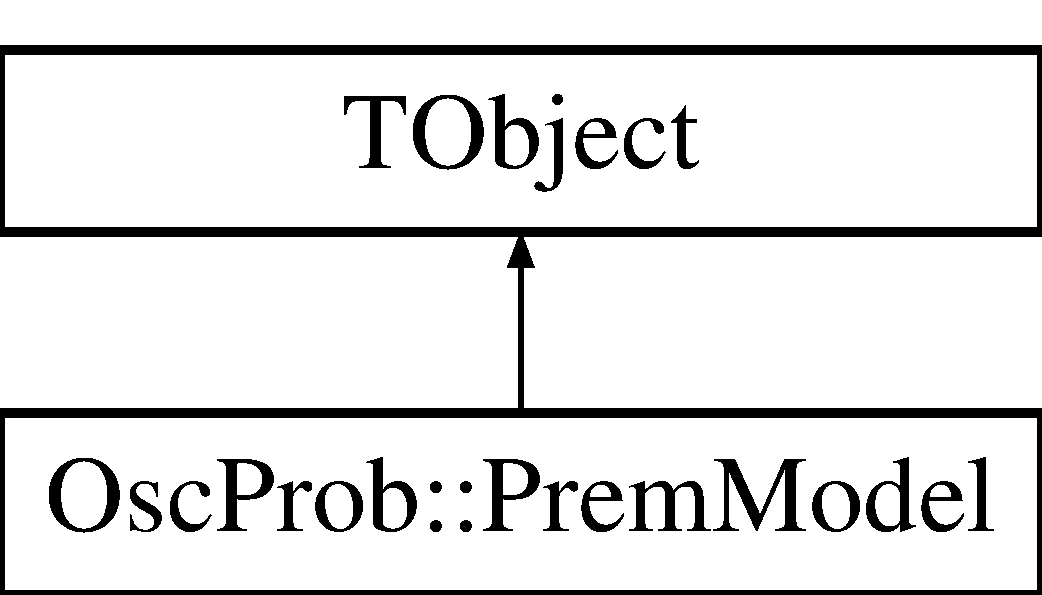
\includegraphics[height=2.000000cm]{classOscProb_1_1PremModel}
\end{center}
\end{figure}
\subsection*{Public Member Functions}
\begin{DoxyCompactItemize}
\item 
\hyperlink{classOscProb_1_1PremModel_a959f8da5c78881b950bd647b67c1ef9b}{Prem\+Model} (std\+::string filename=\char`\"{}\char`\"{})
\begin{DoxyCompactList}\small\item\em Constructor. \end{DoxyCompactList}\item 
virtual \hyperlink{classOscProb_1_1PremModel_aac484ca4e607f2b0fc6f599358cb95fb}{$\sim$\+Prem\+Model} ()
\begin{DoxyCompactList}\small\item\em Destructor. \end{DoxyCompactList}\item 
virtual int \hyperlink{classOscProb_1_1PremModel_ac69162cc5e3c8b7c1b8a85571ff2063b}{Fill\+Path} (double cosT)
\begin{DoxyCompactList}\small\item\em Fill the path sequence in a vector. \end{DoxyCompactList}\item 
virtual std\+::vector$<$ \hyperlink{structOscProb_1_1NuPath}{Osc\+Prob\+::\+Nu\+Path} $>$ \hyperlink{classOscProb_1_1PremModel_adbe7a5df260cba3923f5cbcb8ab2f03f}{Get\+Nu\+Path} ()
\begin{DoxyCompactList}\small\item\em Get the current neutrino path sequence. \end{DoxyCompactList}\item 
virtual std\+::vector$<$ \hyperlink{structOscProb_1_1NuPath}{Osc\+Prob\+::\+Nu\+Path} $>$ \hyperlink{classOscProb_1_1PremModel_a5b6f83f2e9b7087e8faad1f19f00ebd5}{Get\+Merged\+Paths} (double prec=0.\+25)
\begin{DoxyCompactList}\small\item\em Get merged path sequence in a vector. \end{DoxyCompactList}\item 
virtual double \hyperlink{classOscProb_1_1PremModel_ae258b41cca80631e3041f0421b25afeb}{Get\+TotalL} (double cosT)
\begin{DoxyCompactList}\small\item\em Get the total baseline for a given cos\+Theta. \end{DoxyCompactList}\item 
virtual double \hyperlink{classOscProb_1_1PremModel_a5328474bdbb703eb4c9d4df49999cda6}{Get\+CosT} (double L)
\begin{DoxyCompactList}\small\item\em Get the cos\+Theta for a given total baseline. \end{DoxyCompactList}\item 
virtual void \hyperlink{classOscProb_1_1PremModel_ac9887d1af4b3c02925fe3228349f593d}{Set\+Layer\+ZoA} (int layer, double zoa)
\begin{DoxyCompactList}\small\item\em Set Z/A of all layers of a given type. \end{DoxyCompactList}\item 
virtual void \hyperlink{classOscProb_1_1PremModel_a6363a5e711dd8b0d2e684677e585b293}{Load\+Model} (std\+::string filename)
\begin{DoxyCompactList}\small\item\em Load an earth model from a file. \end{DoxyCompactList}\item 
virtual void \hyperlink{classOscProb_1_1PremModel_a55b314e97ed9b92931e08ada0c0947eb}{Set\+Det\+Pos} (double pos)
\begin{DoxyCompactList}\small\item\em Set the detector position in km. \end{DoxyCompactList}\item 
virtual std\+::vector$<$ \hyperlink{structOscProb_1_1PremLayer}{Osc\+Prob\+::\+Prem\+Layer} $>$ \hyperlink{classOscProb_1_1PremModel_ae4feeccc7027253f5c2e2493098145ca}{Get\+Prem\+Layers} ()
\begin{DoxyCompactList}\small\item\em Get the set of earth layers. \end{DoxyCompactList}\item 
virtual \hyperlink{structOscProb_1_1NuPath}{Osc\+Prob\+::\+Nu\+Path} \hyperlink{classOscProb_1_1PremModel_a646977424cdca178a77694397146c2f8}{Avg\+Path} (\hyperlink{structOscProb_1_1NuPath}{Osc\+Prob\+::\+Nu\+Path} p1, \hyperlink{structOscProb_1_1NuPath}{Osc\+Prob\+::\+Nu\+Path} p2)
\begin{DoxyCompactList}\small\item\em Get the average of two paths. \end{DoxyCompactList}\item 
virtual void \hyperlink{classOscProb_1_1PremModel_ac5496d6d5bafcf7740c60838d3eee7b3}{Set\+Remove\+Small\+Paths} (bool rp=true)
\begin{DoxyCompactList}\small\item\em Set tag to remove small paths. \end{DoxyCompactList}\end{DoxyCompactItemize}
\subsection*{Protected Member Functions}
\begin{DoxyCompactItemize}
\item 
virtual void \hyperlink{classOscProb_1_1PremModel_aaead53a9385bda9b0219fd051d0cdd11}{Clear\+Model} ()
\begin{DoxyCompactList}\small\item\em Clear the earth model information. \end{DoxyCompactList}\item 
virtual void \hyperlink{classOscProb_1_1PremModel_a08c337b84138adc46ee4dd002e9262d2}{Add\+Layer} (double radius, double density, double zoa, double layer)
\begin{DoxyCompactList}\small\item\em Add a layer to the model. \end{DoxyCompactList}\item 
virtual void \hyperlink{classOscProb_1_1PremModel_aca013f7ac5494282834048786a0e07a6}{Add\+Path} (double length, \hyperlink{structOscProb_1_1PremLayer}{Prem\+Layer} pl)
\begin{DoxyCompactList}\small\item\em Add a path segment to the sequence. \end{DoxyCompactList}\item 
virtual std\+::vector$<$ \hyperlink{structOscProb_1_1NuPath}{Osc\+Prob\+::\+Nu\+Path} $>$ \hyperlink{classOscProb_1_1PremModel_a87cb8043b58fde2c8a8779e6ae1b5135}{Merge\+Paths} (std\+::vector$<$ \hyperlink{structOscProb_1_1NuPath}{Osc\+Prob\+::\+Nu\+Path} $>$ input\+Path, int j, int k)
\begin{DoxyCompactList}\small\item\em Merge paths j and k in vector. \end{DoxyCompactList}\item 
\hyperlink{classOscProb_1_1PremModel_a9a1d78e29217bb0dd00ae3bd96d22b69}{Class\+Def} (\hyperlink{classOscProb_1_1PremModel}{Prem\+Model}, 1)
\end{DoxyCompactItemize}
\subsection*{Protected Attributes}
\begin{DoxyCompactItemize}
\item 
std\+::vector$<$ \hyperlink{structOscProb_1_1PremLayer}{Osc\+Prob\+::\+Prem\+Layer} $>$ \hyperlink{classOscProb_1_1PremModel_a19a9a3b23ec154ad7a29f92b74aa5bc6}{f\+Prem\+Layers}
\begin{DoxyCompactList}\small\item\em The layers in the earth model. \end{DoxyCompactList}\item 
std\+::vector$<$ \hyperlink{structOscProb_1_1NuPath}{Osc\+Prob\+::\+Nu\+Path} $>$ \hyperlink{classOscProb_1_1PremModel_aaf3c77e35798d664853157013c90ad2b}{f\+Nu\+Path}
\begin{DoxyCompactList}\small\item\em The current neutrino path sequence. \end{DoxyCompactList}\item 
int \hyperlink{classOscProb_1_1PremModel_a4fb68506493666349f418b893a996185}{f\+Det\+Layer}
\begin{DoxyCompactList}\small\item\em The layer index of the detector. \end{DoxyCompactList}\item 
double \hyperlink{classOscProb_1_1PremModel_ab12ea0343cd11b9233ffd20ab5e620c7}{f\+Det\+Pos}
\begin{DoxyCompactList}\small\item\em The radius where the detector lives. \end{DoxyCompactList}\item 
bool \hyperlink{classOscProb_1_1PremModel_a3973df6f5f2ff219cd2f865b31aacfd2}{f\+Remove\+Small\+Paths}
\begin{DoxyCompactList}\small\item\em Tag whether to merge small paths. \end{DoxyCompactList}\end{DoxyCompactItemize}
\subsection*{Static Protected Attributes}
\begin{DoxyCompactItemize}
\item 
static const double \hyperlink{classOscProb_1_1PremModel_a8ad1335ebe80ee1cd1cdf59d774ab34b}{D\+E\+T\+\_\+\+T\+OL} = 0.\+2
\begin{DoxyCompactList}\small\item\em The detector position tolerance near boundaries. \end{DoxyCompactList}\end{DoxyCompactItemize}


\subsection{Detailed Description}
This class implements a spherically symmetric model of the earth using \hyperlink{structOscProb_1_1PremLayer}{Prem\+Layer}\textquotesingle{}s to store spherical shells with different properties.

The class is then able to produce path sequences through the different earth layers as a function of the cosine of the zenith angle with respect to the detector.

The detector can be positioned at any radius within the model and the path sequences will take into account the fact that some layers are above the detector.

By default this implements the model stored in Prem\+Tables/prem\+\_\+default.\+txt with the detector at the bottom of the ocean layer (radius = 6368 km).

This class inherits from T\+Object and can be saved in R\+O\+OT files.

\begin{DoxyAuthor}{Author}
jcoelho@apc.\+in2p3.\+fr 
\end{DoxyAuthor}


Definition at line 37 of file Prem\+Model.\+h.



\subsection{Constructor \& Destructor Documentation}
\mbox{\Hypertarget{classOscProb_1_1PremModel_a959f8da5c78881b950bd647b67c1ef9b}\label{classOscProb_1_1PremModel_a959f8da5c78881b950bd647b67c1ef9b}} 
\index{Osc\+Prob\+::\+Prem\+Model@{Osc\+Prob\+::\+Prem\+Model}!Prem\+Model@{Prem\+Model}}
\index{Prem\+Model@{Prem\+Model}!Osc\+Prob\+::\+Prem\+Model@{Osc\+Prob\+::\+Prem\+Model}}
\subsubsection{\texorpdfstring{Prem\+Model()}{PremModel()}}
{\footnotesize\ttfamily Prem\+Model\+::\+Prem\+Model (\begin{DoxyParamCaption}\item[{std\+::string}]{filename = {\ttfamily \char`\"{}\char`\"{}} }\end{DoxyParamCaption})}

Constructor.

By default this implements the model stored in Prem\+Tables/prem\+\_\+default.\+txt with the detector at the bottom of the ocean layer (radius = 6368 km).


\begin{DoxyParams}{Parameters}
{\em filename} & -\/ The txt file containing a table of earth layers \\
\hline
\end{DoxyParams}


Definition at line 35 of file Prem\+Model.\+cxx.



References Load\+Model(), and Set\+Det\+Pos().


\begin{DoxyCode}
35                                     :
36 \hyperlink{classOscProb_1_1PremModel_a4fb68506493666349f418b893a996185}{fDetLayer}(0), \hyperlink{classOscProb_1_1PremModel_a3973df6f5f2ff219cd2f865b31aacfd2}{fRemoveSmallPaths}(\textcolor{keyword}{false})
37 \{
38 
39   \hyperlink{classOscProb_1_1PremModel_a55b314e97ed9b92931e08ada0c0947eb}{SetDetPos}(6368);
40   \hyperlink{classOscProb_1_1PremModel_a6363a5e711dd8b0d2e684677e585b293}{LoadModel}(filename);
41 
42 \}
\end{DoxyCode}
\mbox{\Hypertarget{classOscProb_1_1PremModel_aac484ca4e607f2b0fc6f599358cb95fb}\label{classOscProb_1_1PremModel_aac484ca4e607f2b0fc6f599358cb95fb}} 
\index{Osc\+Prob\+::\+Prem\+Model@{Osc\+Prob\+::\+Prem\+Model}!````~Prem\+Model@{$\sim$\+Prem\+Model}}
\index{````~Prem\+Model@{$\sim$\+Prem\+Model}!Osc\+Prob\+::\+Prem\+Model@{Osc\+Prob\+::\+Prem\+Model}}
\subsubsection{\texorpdfstring{$\sim$\+Prem\+Model()}{~PremModel()}}
{\footnotesize\ttfamily Prem\+Model\+::$\sim$\+Prem\+Model (\begin{DoxyParamCaption}{ }\end{DoxyParamCaption})\hspace{0.3cm}{\ttfamily [virtual]}}

Nothing to clean. 

Definition at line 48 of file Prem\+Model.\+cxx.


\begin{DoxyCode}
48 \{\}
\end{DoxyCode}


\subsection{Member Function Documentation}
\mbox{\Hypertarget{classOscProb_1_1PremModel_a08c337b84138adc46ee4dd002e9262d2}\label{classOscProb_1_1PremModel_a08c337b84138adc46ee4dd002e9262d2}} 
\index{Osc\+Prob\+::\+Prem\+Model@{Osc\+Prob\+::\+Prem\+Model}!Add\+Layer@{Add\+Layer}}
\index{Add\+Layer@{Add\+Layer}!Osc\+Prob\+::\+Prem\+Model@{Osc\+Prob\+::\+Prem\+Model}}
\subsubsection{\texorpdfstring{Add\+Layer()}{AddLayer()}}
{\footnotesize\ttfamily void Prem\+Model\+::\+Add\+Layer (\begin{DoxyParamCaption}\item[{double}]{radius,  }\item[{double}]{density,  }\item[{double}]{zoa,  }\item[{double}]{layer }\end{DoxyParamCaption})\hspace{0.3cm}{\ttfamily [protected]}, {\ttfamily [virtual]}}

Add a layer to the earth model.


\begin{DoxyParams}{Parameters}
{\em radius} & -\/ The outer radius of the layer in km \\
\hline
{\em density} & -\/ The density of the layer in g/cm$^\wedge$3 \\
\hline
{\em zoa} & -\/ The effective Z/A value of the layer \\
\hline
{\em layer} & -\/ An index to identify the matter type (e.\+g. earth inner core) \\
\hline
\end{DoxyParams}


Definition at line 105 of file Prem\+Model.\+cxx.



References f\+Prem\+Layers.



Referenced by Load\+Model().


\begin{DoxyCode}
107 \{
108 
109   \hyperlink{classOscProb_1_1PremModel_a19a9a3b23ec154ad7a29f92b74aa5bc6}{fPremLayers}.push\_back( \hyperlink{structOscProb_1_1PremLayer}{PremLayer}(radius, density, zoa, layer) );
110   
111 \}
\end{DoxyCode}
\mbox{\Hypertarget{classOscProb_1_1PremModel_aca013f7ac5494282834048786a0e07a6}\label{classOscProb_1_1PremModel_aca013f7ac5494282834048786a0e07a6}} 
\index{Osc\+Prob\+::\+Prem\+Model@{Osc\+Prob\+::\+Prem\+Model}!Add\+Path@{Add\+Path}}
\index{Add\+Path@{Add\+Path}!Osc\+Prob\+::\+Prem\+Model@{Osc\+Prob\+::\+Prem\+Model}}
\subsubsection{\texorpdfstring{Add\+Path()}{AddPath()}}
{\footnotesize\ttfamily void Prem\+Model\+::\+Add\+Path (\begin{DoxyParamCaption}\item[{double}]{length,  }\item[{\hyperlink{structOscProb_1_1PremLayer}{Prem\+Layer}}]{pl }\end{DoxyParamCaption})\hspace{0.3cm}{\ttfamily [protected]}, {\ttfamily [virtual]}}

Add a path segment to the sequence.

For a given \hyperlink{structOscProb_1_1PremLayer}{Prem\+Layer}, adds a path of a given length in that material


\begin{DoxyParams}{Parameters}
{\em length} & -\/ The length of the path segment in km \\
\hline
{\em pl} & -\/ The layer we are crossing \\
\hline
\end{DoxyParams}


Definition at line 269 of file Prem\+Model.\+cxx.



References Osc\+Prob\+::\+Prem\+Layer\+::density, f\+Nu\+Path, Osc\+Prob\+::\+Prem\+Layer\+::layer, and Osc\+Prob\+::\+Prem\+Layer\+::zoa.



Referenced by Fill\+Path().


\begin{DoxyCode}
270 \{
271 
272   \hyperlink{classOscProb_1_1PremModel_aaf3c77e35798d664853157013c90ad2b}{fNuPath}.push\_back( \hyperlink{structOscProb_1_1NuPath}{NuPath}(length, pl.\hyperlink{structOscProb_1_1PremLayer_aba2536cbdab87d0db33df47f95c4f2c3}{density}, pl.\hyperlink{structOscProb_1_1PremLayer_a8687a8169d786fca79908292d11077f5}{zoa}, pl.
      \hyperlink{structOscProb_1_1PremLayer_aca8d7df68e6f982155b68b7e6a7ef389}{layer}) );
273   
274 \}
\end{DoxyCode}
\mbox{\Hypertarget{classOscProb_1_1PremModel_a646977424cdca178a77694397146c2f8}\label{classOscProb_1_1PremModel_a646977424cdca178a77694397146c2f8}} 
\index{Osc\+Prob\+::\+Prem\+Model@{Osc\+Prob\+::\+Prem\+Model}!Avg\+Path@{Avg\+Path}}
\index{Avg\+Path@{Avg\+Path}!Osc\+Prob\+::\+Prem\+Model@{Osc\+Prob\+::\+Prem\+Model}}
\subsubsection{\texorpdfstring{Avg\+Path()}{AvgPath()}}
{\footnotesize\ttfamily \hyperlink{structOscProb_1_1NuPath}{Nu\+Path} Prem\+Model\+::\+Avg\+Path (\begin{DoxyParamCaption}\item[{\hyperlink{structOscProb_1_1NuPath}{Osc\+Prob\+::\+Nu\+Path}}]{p1,  }\item[{\hyperlink{structOscProb_1_1NuPath}{Osc\+Prob\+::\+Nu\+Path}}]{p2 }\end{DoxyParamCaption})\hspace{0.3cm}{\ttfamily [virtual]}}

Get the merged average of two paths

This method will merge two paths and take their average density weighted by Z/A and path length.

The Z/A of the first path will be kept in the merged path


\begin{DoxyParams}{Parameters}
{\em p1} & -\/ The first path to merge \\
\hline
{\em p2} & -\/ The second path to merge \\
\hline
\end{DoxyParams}
\begin{DoxyReturn}{Returns}
The merged path 
\end{DoxyReturn}


Definition at line 463 of file Prem\+Model.\+cxx.



References Osc\+Prob\+::\+Nu\+Path\+::density, Osc\+Prob\+::\+Nu\+Path\+::length, and Osc\+Prob\+::\+Nu\+Path\+::zoa.



Referenced by Get\+Merged\+Paths(), and Merge\+Paths().


\begin{DoxyCode}
463                                              \{
464 
465   \textcolor{comment}{// Start with the first path}
466   \hyperlink{structOscProb_1_1NuPath}{NuPath} mergedPath = p1;
467 
468   \textcolor{comment}{// Add the second length}
469   mergedPath.\hyperlink{structOscProb_1_1NuPath_af22660894b6e25cf835500381b155557}{length} += p2.\hyperlink{structOscProb_1_1NuPath_af22660894b6e25cf835500381b155557}{length};
470 
471   \textcolor{comment}{// Compute weighted average of density}
472   mergedPath.\hyperlink{structOscProb_1_1NuPath_a54ddd451db69bc54434de3cf18a117ca}{density} = (p1.\hyperlink{structOscProb_1_1NuPath_a54ddd451db69bc54434de3cf18a117ca}{density}*p1.\hyperlink{structOscProb_1_1NuPath_af3213f3691ba83c6bc05f4a3490f6b31}{zoa}*p1.\hyperlink{structOscProb_1_1NuPath_af22660894b6e25cf835500381b155557}{length} + p2.
      \hyperlink{structOscProb_1_1NuPath_a54ddd451db69bc54434de3cf18a117ca}{density}*p2.\hyperlink{structOscProb_1_1NuPath_af3213f3691ba83c6bc05f4a3490f6b31}{zoa}*p2.\hyperlink{structOscProb_1_1NuPath_af22660894b6e25cf835500381b155557}{length}) / (p1.\hyperlink{structOscProb_1_1NuPath_af3213f3691ba83c6bc05f4a3490f6b31}{zoa}*p1.\hyperlink{structOscProb_1_1NuPath_af22660894b6e25cf835500381b155557}{length} + p2.\hyperlink{structOscProb_1_1NuPath_af3213f3691ba83c6bc05f4a3490f6b31}{zoa}*p2.
      \hyperlink{structOscProb_1_1NuPath_af22660894b6e25cf835500381b155557}{length});
473 
474   \textcolor{comment}{// return merged path}
475   \textcolor{keywordflow}{return} mergedPath;
476 
477 \}
\end{DoxyCode}
\mbox{\Hypertarget{classOscProb_1_1PremModel_a9a1d78e29217bb0dd00ae3bd96d22b69}\label{classOscProb_1_1PremModel_a9a1d78e29217bb0dd00ae3bd96d22b69}} 
\index{Osc\+Prob\+::\+Prem\+Model@{Osc\+Prob\+::\+Prem\+Model}!Class\+Def@{Class\+Def}}
\index{Class\+Def@{Class\+Def}!Osc\+Prob\+::\+Prem\+Model@{Osc\+Prob\+::\+Prem\+Model}}
\subsubsection{\texorpdfstring{Class\+Def()}{ClassDef()}}
{\footnotesize\ttfamily Osc\+Prob\+::\+Prem\+Model\+::\+Class\+Def (\begin{DoxyParamCaption}\item[{\hyperlink{classOscProb_1_1PremModel}{Prem\+Model}}]{,  }\item[{1}]{ }\end{DoxyParamCaption})\hspace{0.3cm}{\ttfamily [protected]}}

\mbox{\Hypertarget{classOscProb_1_1PremModel_aaead53a9385bda9b0219fd051d0cdd11}\label{classOscProb_1_1PremModel_aaead53a9385bda9b0219fd051d0cdd11}} 
\index{Osc\+Prob\+::\+Prem\+Model@{Osc\+Prob\+::\+Prem\+Model}!Clear\+Model@{Clear\+Model}}
\index{Clear\+Model@{Clear\+Model}!Osc\+Prob\+::\+Prem\+Model@{Osc\+Prob\+::\+Prem\+Model}}
\subsubsection{\texorpdfstring{Clear\+Model()}{ClearModel()}}
{\footnotesize\ttfamily void Prem\+Model\+::\+Clear\+Model (\begin{DoxyParamCaption}{ }\end{DoxyParamCaption})\hspace{0.3cm}{\ttfamily [protected]}, {\ttfamily [virtual]}}

Clear the earth model information. 

Definition at line 88 of file Prem\+Model.\+cxx.



References f\+Det\+Layer, and f\+Prem\+Layers.



Referenced by Load\+Model().


\begin{DoxyCode}
89 \{
90 
91   \hyperlink{classOscProb_1_1PremModel_a4fb68506493666349f418b893a996185}{fDetLayer} = 0;
92   \hyperlink{classOscProb_1_1PremModel_a19a9a3b23ec154ad7a29f92b74aa5bc6}{fPremLayers}.clear();
93 
94 \}
\end{DoxyCode}
\mbox{\Hypertarget{classOscProb_1_1PremModel_ac69162cc5e3c8b7c1b8a85571ff2063b}\label{classOscProb_1_1PremModel_ac69162cc5e3c8b7c1b8a85571ff2063b}} 
\index{Osc\+Prob\+::\+Prem\+Model@{Osc\+Prob\+::\+Prem\+Model}!Fill\+Path@{Fill\+Path}}
\index{Fill\+Path@{Fill\+Path}!Osc\+Prob\+::\+Prem\+Model@{Osc\+Prob\+::\+Prem\+Model}}
\subsubsection{\texorpdfstring{Fill\+Path()}{FillPath()}}
{\footnotesize\ttfamily int Prem\+Model\+::\+Fill\+Path (\begin{DoxyParamCaption}\item[{double}]{cosT }\end{DoxyParamCaption})\hspace{0.3cm}{\ttfamily [virtual]}}

Fill the path sequence in a vector.

This will start at the upper-\/most layer and find straight paths to the boundary of the next layer down. When reaching the inner-\/most layer in the given direction, the paths move back to outer layers until hitting the detector.

The path sequence is stored as an attribute and can be retrieved with the function Get\+Nu\+Path.


\begin{DoxyParams}{Parameters}
{\em cosT} & -\/ The cosine of the neutrino direction \\
\hline
\end{DoxyParams}
\begin{DoxyReturn}{Returns}
The number of path segments in the sequence 
\end{DoxyReturn}


Definition at line 291 of file Prem\+Model.\+cxx.



References Add\+Path(), f\+Det\+Layer, f\+Nu\+Path, and f\+Prem\+Layers.


\begin{DoxyCode}
292 \{
293 
294   \textcolor{comment}{// Clear current path sequence}
295   \hyperlink{classOscProb_1_1PremModel_aaf3c77e35798d664853157013c90ad2b}{fNuPath}.clear();
296   
297   \textcolor{comment}{// Do nothing if cosine is unphysical}
298   \textcolor{keywordflow}{if}(fabs(cosT) > 1) \textcolor{keywordflow}{return} 0;
299 
300   \textcolor{comment}{// Define the minimum path radius}
301   \textcolor{keywordtype}{double} minR = \hyperlink{classOscProb_1_1PremModel_a19a9a3b23ec154ad7a29f92b74aa5bc6}{fPremLayers}[\hyperlink{classOscProb_1_1PremModel_a4fb68506493666349f418b893a996185}{fDetLayer}].radius * sqrt(1 - cosT*cosT);
302 
303   \textcolor{comment}{// Set the top layer index}
304   \textcolor{keywordtype}{int} toplayer = \hyperlink{classOscProb_1_1PremModel_a19a9a3b23ec154ad7a29f92b74aa5bc6}{fPremLayers}.size() - 1;
305   
306   \textcolor{comment}{// Find the inner-most crossed layer}
307   \textcolor{keywordtype}{int} minlayer = 0;
308   \textcolor{keywordflow}{while}(\hyperlink{classOscProb_1_1PremModel_a19a9a3b23ec154ad7a29f92b74aa5bc6}{fPremLayers}[minlayer].radius < minR) minlayer++; 
309 
310   \textcolor{comment}{// Compute the number of path segments needed}
311   \textcolor{keywordtype}{int} nsteps = toplayer - \hyperlink{classOscProb_1_1PremModel_a4fb68506493666349f418b893a996185}{fDetLayer};
312   \textcolor{keywordflow}{if}(cosT < 0) nsteps += 2*(fDetLayer - minlayer) + 1;
313 
314   \textcolor{comment}{// Start at the top layer and go down}
315   \textcolor{keywordtype}{int} layer = toplayer;
316   \textcolor{keywordtype}{int} dl = -1;
317   
318   \textcolor{comment}{// Loop over all path segments}
319   \textcolor{keywordflow}{for}(\textcolor{keywordtype}{int} i=0; i<nsteps; i++)\{
320   
321     \textcolor{comment}{// Get square of the path length between this layer's }
322     \textcolor{comment}{// outer radius and  inner-most radius}
323     \textcolor{keywordtype}{double} L1 = pow(\hyperlink{classOscProb_1_1PremModel_a19a9a3b23ec154ad7a29f92b74aa5bc6}{fPremLayers}[layer].radius,2) - minR*minR;
324 
325     \textcolor{comment}{// If L1 is negative, outer radius is not crossed.}
326     \textcolor{comment}{// This only happens if detector is at the top layer and the}
327     \textcolor{comment}{// neutrino is coming from above.}
328     \textcolor{keywordflow}{if}(L1 < 0) \textcolor{keywordflow}{return} \textcolor{keyword}{true};
329     
330     \textcolor{comment}{// Get square of the path length between this layer's }
331     \textcolor{comment}{// inner radius and  inner-most radius}
332     \textcolor{keywordtype}{double} L2 = -minR*minR;
333     \textcolor{keywordflow}{if}(layer>0) L2 += pow(\hyperlink{classOscProb_1_1PremModel_a19a9a3b23ec154ad7a29f92b74aa5bc6}{fPremLayers}[layer-1].radius,2);
334     
335     \textcolor{comment}{// If L2 is negative, inner radius is not crossed,}
336     \textcolor{comment}{// so set this as the minimum layer.}
337     \textcolor{keywordtype}{bool} ismin = (L2<=0 && cosT < 0);
338 
339     \textcolor{comment}{// Store the path segment length}
340     \textcolor{keywordtype}{double} dL;
341     
342     \textcolor{comment}{// If it's the minimum layer, connect two outer radius }
343     \textcolor{comment}{// crossing points. If not, compute difference between}
344     \textcolor{comment}{// inner and outer radius crossings.}
345     \textcolor{keywordflow}{if}(ismin)      dL = 2 * sqrt(L1);
346     \textcolor{keywordflow}{else} \textcolor{keywordflow}{if}(L2>=0) dL = sqrt(L1) - sqrt(L2);
347     \textcolor{keywordflow}{else}           dL = sqrt(L1); \textcolor{comment}{// This should never actually happen,}
348                                   \textcolor{comment}{// but protect in case L2 is slightly}
349                                   \textcolor{comment}{// negative when it should be zero.}
350                                   \textcolor{comment}{// e.g. arriving at the detector from above.}
351     
352     \textcolor{comment}{// Add this path segment to the sequence}
353     \hyperlink{classOscProb_1_1PremModel_aca013f7ac5494282834048786a0e07a6}{AddPath}(dL, \hyperlink{classOscProb_1_1PremModel_a19a9a3b23ec154ad7a29f92b74aa5bc6}{fPremLayers}[layer]);
354     
355     \textcolor{comment}{// If we reached the inner-most layer,}
356     \textcolor{comment}{// start moving up again.}
357     \textcolor{keywordflow}{if}(ismin) dl = 1;
358     
359     \textcolor{comment}{// Move to next layer}
360     layer += dl;
361   
362   \}
363 
364   \textcolor{comment}{// Return the number of path segments}
365   \textcolor{keywordflow}{return} \hyperlink{classOscProb_1_1PremModel_aaf3c77e35798d664853157013c90ad2b}{fNuPath}.size();
366 
367 \}
\end{DoxyCode}
\mbox{\Hypertarget{classOscProb_1_1PremModel_a5328474bdbb703eb4c9d4df49999cda6}\label{classOscProb_1_1PremModel_a5328474bdbb703eb4c9d4df49999cda6}} 
\index{Osc\+Prob\+::\+Prem\+Model@{Osc\+Prob\+::\+Prem\+Model}!Get\+CosT@{Get\+CosT}}
\index{Get\+CosT@{Get\+CosT}!Osc\+Prob\+::\+Prem\+Model@{Osc\+Prob\+::\+Prem\+Model}}
\subsubsection{\texorpdfstring{Get\+Cos\+T()}{GetCosT()}}
{\footnotesize\ttfamily double Prem\+Model\+::\+Get\+CosT (\begin{DoxyParamCaption}\item[{double}]{L }\end{DoxyParamCaption})\hspace{0.3cm}{\ttfamily [virtual]}}

Get the cos\+Theta for a given total baseline.

Given a baseline, find the direction of the neutrino. This could be useful for experiments with fixed baselines for example.

The baseline must be within the range of possible values in this earth model. Will return vertical neutrinos otherwise.


\begin{DoxyParams}{Parameters}
{\em L} & -\/ The total baseline of the neutrino \\
\hline
\end{DoxyParams}


Definition at line 247 of file Prem\+Model.\+cxx.



References f\+Det\+Layer, and f\+Prem\+Layers.


\begin{DoxyCode}
248 \{
249 
250   \textcolor{keywordtype}{double} rAbove = \hyperlink{classOscProb_1_1PremModel_a19a9a3b23ec154ad7a29f92b74aa5bc6}{fPremLayers}.back().radius;     \textcolor{comment}{// Radius above detector}
251   \textcolor{keywordtype}{double} rBelow = \hyperlink{classOscProb_1_1PremModel_a19a9a3b23ec154ad7a29f92b74aa5bc6}{fPremLayers}[\hyperlink{classOscProb_1_1PremModel_a4fb68506493666349f418b893a996185}{fDetLayer}].radius; \textcolor{comment}{// Radius below detector}
252   
253   \textcolor{keywordflow}{if}(L < rAbove - rBelow) \textcolor{keywordflow}{return}  1;
254   \textcolor{keywordflow}{if}(L > rAbove + rBelow) \textcolor{keywordflow}{return} -1;
255   
256   \textcolor{keywordflow}{return} (rAbove*rAbove - rBelow*rBelow - L*L) / (2*rBelow*L);
257   
258 \}
\end{DoxyCode}
\mbox{\Hypertarget{classOscProb_1_1PremModel_a5b6f83f2e9b7087e8faad1f19f00ebd5}\label{classOscProb_1_1PremModel_a5b6f83f2e9b7087e8faad1f19f00ebd5}} 
\index{Osc\+Prob\+::\+Prem\+Model@{Osc\+Prob\+::\+Prem\+Model}!Get\+Merged\+Paths@{Get\+Merged\+Paths}}
\index{Get\+Merged\+Paths@{Get\+Merged\+Paths}!Osc\+Prob\+::\+Prem\+Model@{Osc\+Prob\+::\+Prem\+Model}}
\subsubsection{\texorpdfstring{Get\+Merged\+Paths()}{GetMergedPaths()}}
{\footnotesize\ttfamily vector$<$ \hyperlink{structOscProb_1_1NuPath}{Nu\+Path} $>$ Prem\+Model\+::\+Get\+Merged\+Paths (\begin{DoxyParamCaption}\item[{double}]{prec = {\ttfamily 0.25} }\end{DoxyParamCaption})\hspace{0.3cm}{\ttfamily [virtual]}}

Merge similar paths to reduce number of steps

This method will merge consecutive paths and take their averages until it finds a large enough gap to start a new merged path.

The merged paths will be returned, and the original detailed path will not be changed and will stay stored as an attribute.


\begin{DoxyParams}{Parameters}
{\em prec} & -\/ The precision to merge paths in g/cm$^\wedge$3 \\
\hline
\end{DoxyParams}
\begin{DoxyReturn}{Returns}
The vector of merged path segments 
\end{DoxyReturn}


Definition at line 382 of file Prem\+Model.\+cxx.



References Avg\+Path(), Osc\+Prob\+::\+Nu\+Path\+::density, f\+Nu\+Path, f\+Remove\+Small\+Paths, Merge\+Paths(), and Osc\+Prob\+::\+Nu\+Path\+::zoa.


\begin{DoxyCode}
382                                                    \{
383 
384   \textcolor{comment}{// The output vector}
385   vector<NuPath> mergedPath;
386 
387   \textcolor{comment}{// Start with the first path}
388   \hyperlink{structOscProb_1_1NuPath}{OscProb::NuPath} path = \hyperlink{classOscProb_1_1PremModel_aaf3c77e35798d664853157013c90ad2b}{fNuPath}[0];
389 
390   \textcolor{comment}{// Track the total length}
391   \textcolor{keywordtype}{double} totL = 0;
392 
393   \textcolor{comment}{// Loop over all paths starting from second}
394   \textcolor{keywordflow}{for}(\textcolor{keywordtype}{int} i=1; i<\hyperlink{classOscProb_1_1PremModel_aaf3c77e35798d664853157013c90ad2b}{fNuPath}.size(); i++)\{
395 
396     \textcolor{comment}{// If this path electron density is beyond the tolerance}
397     \textcolor{keywordflow}{if}( fabs(path.\hyperlink{structOscProb_1_1NuPath_a54ddd451db69bc54434de3cf18a117ca}{density}*path.\hyperlink{structOscProb_1_1NuPath_af3213f3691ba83c6bc05f4a3490f6b31}{zoa} - \hyperlink{classOscProb_1_1PremModel_aaf3c77e35798d664853157013c90ad2b}{fNuPath}[i].density*\hyperlink{classOscProb_1_1PremModel_aaf3c77e35798d664853157013c90ad2b}{fNuPath}[i].zoa) > prec*path
      .\hyperlink{structOscProb_1_1NuPath_af3213f3691ba83c6bc05f4a3490f6b31}{zoa} )\{
398 
399       \textcolor{comment}{// Add merged path to vector}
400       mergedPath.push\_back(path);
401       
402       \textcolor{comment}{// Set this path as new merged path}
403       path = \hyperlink{classOscProb_1_1PremModel_aaf3c77e35798d664853157013c90ad2b}{fNuPath}[i];
404 
405     \}
406     \textcolor{comment}{// If path is within tolerance}
407     \textcolor{keywordflow}{else}\{
408       
409       \textcolor{comment}{// Merge the path with current merged path}
410       path = \hyperlink{classOscProb_1_1PremModel_a646977424cdca178a77694397146c2f8}{AvgPath}(path, \hyperlink{classOscProb_1_1PremModel_aaf3c77e35798d664853157013c90ad2b}{fNuPath}[i]);
411 
412     \}
413 
414     \textcolor{comment}{// Increment total length}
415     totL += \hyperlink{classOscProb_1_1PremModel_aaf3c77e35798d664853157013c90ad2b}{fNuPath}[i].length;
416 
417   \}\textcolor{comment}{// End of loop over paths}
418 
419   \textcolor{comment}{// Add the final merged path to vector}
420   mergedPath.push\_back(path);
421 
422   \textcolor{comment}{// If tag is true, remove small paths}
423   \textcolor{keywordflow}{if}(\hyperlink{classOscProb_1_1PremModel_a3973df6f5f2ff219cd2f865b31aacfd2}{fRemoveSmallPaths})\{
424 
425     \textcolor{comment}{// Start at first path}
426     \textcolor{keywordtype}{int} k = 0;
427 
428     \textcolor{comment}{// While not at the end of vector}
429     \textcolor{keywordflow}{while}(k + 1 < mergedPath.size())\{
430 
431       \textcolor{comment}{// If length is less than 1% of total}
432       \textcolor{keywordflow}{if}(mergedPath[k].length < 0.01*totL)\{
433 
434         \textcolor{comment}{// Merge path with following path}
435         mergedPath = \hyperlink{classOscProb_1_1PremModel_a87cb8043b58fde2c8a8779e6ae1b5135}{MergePaths}(mergedPath, k, k+1);
436 
437       \}
438       \textcolor{comment}{// If path is long enough skip it}
439       \textcolor{keywordflow}{else} k++;
440 
441     \}\textcolor{comment}{// End of while loop}
442 
443   \}\textcolor{comment}{// End of if statement}
444 
445   \textcolor{comment}{// return the merged vector}
446   \textcolor{keywordflow}{return} mergedPath;
447 
448 \}
\end{DoxyCode}
\mbox{\Hypertarget{classOscProb_1_1PremModel_adbe7a5df260cba3923f5cbcb8ab2f03f}\label{classOscProb_1_1PremModel_adbe7a5df260cba3923f5cbcb8ab2f03f}} 
\index{Osc\+Prob\+::\+Prem\+Model@{Osc\+Prob\+::\+Prem\+Model}!Get\+Nu\+Path@{Get\+Nu\+Path}}
\index{Get\+Nu\+Path@{Get\+Nu\+Path}!Osc\+Prob\+::\+Prem\+Model@{Osc\+Prob\+::\+Prem\+Model}}
\subsubsection{\texorpdfstring{Get\+Nu\+Path()}{GetNuPath()}}
{\footnotesize\ttfamily vector$<$ \hyperlink{structOscProb_1_1NuPath}{Nu\+Path} $>$ Prem\+Model\+::\+Get\+Nu\+Path (\begin{DoxyParamCaption}{ }\end{DoxyParamCaption})\hspace{0.3cm}{\ttfamily [virtual]}}

Get the current neutrino path sequence

The path needs to be filled for a given cos\+Theta before calling this function. 

Definition at line 73 of file Prem\+Model.\+cxx.



References f\+Nu\+Path.


\begin{DoxyCode}
73 \{ \textcolor{keywordflow}{return} \hyperlink{classOscProb_1_1PremModel_aaf3c77e35798d664853157013c90ad2b}{fNuPath}; \}
\end{DoxyCode}
\mbox{\Hypertarget{classOscProb_1_1PremModel_ae4feeccc7027253f5c2e2493098145ca}\label{classOscProb_1_1PremModel_ae4feeccc7027253f5c2e2493098145ca}} 
\index{Osc\+Prob\+::\+Prem\+Model@{Osc\+Prob\+::\+Prem\+Model}!Get\+Prem\+Layers@{Get\+Prem\+Layers}}
\index{Get\+Prem\+Layers@{Get\+Prem\+Layers}!Osc\+Prob\+::\+Prem\+Model@{Osc\+Prob\+::\+Prem\+Model}}
\subsubsection{\texorpdfstring{Get\+Prem\+Layers()}{GetPremLayers()}}
{\footnotesize\ttfamily vector$<$ \hyperlink{structOscProb_1_1PremLayer}{Prem\+Layer} $>$ Prem\+Model\+::\+Get\+Prem\+Layers (\begin{DoxyParamCaption}{ }\end{DoxyParamCaption})\hspace{0.3cm}{\ttfamily [virtual]}}

Get the set of earth layers

This returns the set of \hyperlink{structOscProb_1_1PremLayer}{Prem\+Layer}\textquotesingle{}s for this earth model and detector position. 

Definition at line 82 of file Prem\+Model.\+cxx.



References f\+Prem\+Layers.


\begin{DoxyCode}
82 \{ \textcolor{keywordflow}{return} \hyperlink{classOscProb_1_1PremModel_a19a9a3b23ec154ad7a29f92b74aa5bc6}{fPremLayers}; \}
\end{DoxyCode}
\mbox{\Hypertarget{classOscProb_1_1PremModel_ae258b41cca80631e3041f0421b25afeb}\label{classOscProb_1_1PremModel_ae258b41cca80631e3041f0421b25afeb}} 
\index{Osc\+Prob\+::\+Prem\+Model@{Osc\+Prob\+::\+Prem\+Model}!Get\+TotalL@{Get\+TotalL}}
\index{Get\+TotalL@{Get\+TotalL}!Osc\+Prob\+::\+Prem\+Model@{Osc\+Prob\+::\+Prem\+Model}}
\subsubsection{\texorpdfstring{Get\+Total\+L()}{GetTotalL()}}
{\footnotesize\ttfamily double Prem\+Model\+::\+Get\+TotalL (\begin{DoxyParamCaption}\item[{double}]{cosT }\end{DoxyParamCaption})\hspace{0.3cm}{\ttfamily [virtual]}}

Get the total baseline for a given cos\+Theta.

The total baseline contains both from above and below the detector.


\begin{DoxyParams}{Parameters}
{\em cosT} & -\/ The cosine of the neutrino direction \\
\hline
\end{DoxyParams}


Definition at line 221 of file Prem\+Model.\+cxx.



References f\+Det\+Layer, and f\+Prem\+Layers.


\begin{DoxyCode}
222 \{
223 
224   \textcolor{keywordflow}{if}(fabs(cosT) > 1) \textcolor{keywordflow}{return} 0;
225 
226   \textcolor{keywordtype}{double} rAbove = \hyperlink{classOscProb_1_1PremModel_a19a9a3b23ec154ad7a29f92b74aa5bc6}{fPremLayers}.back().radius;     \textcolor{comment}{// Radius above detector}
227   \textcolor{keywordtype}{double} rBelow = \hyperlink{classOscProb_1_1PremModel_a19a9a3b23ec154ad7a29f92b74aa5bc6}{fPremLayers}[\hyperlink{classOscProb_1_1PremModel_a4fb68506493666349f418b893a996185}{fDetLayer}].radius; \textcolor{comment}{// Radius below detector}
228 
229   \textcolor{keywordtype}{double} sinsqrT = 1 - cosT*cosT;
230 
231   \textcolor{keywordflow}{return} -rBelow*cosT + sqrt(rAbove*rAbove - rBelow*rBelow*sinsqrT);
232 
233 \}
\end{DoxyCode}
\mbox{\Hypertarget{classOscProb_1_1PremModel_a6363a5e711dd8b0d2e684677e585b293}\label{classOscProb_1_1PremModel_a6363a5e711dd8b0d2e684677e585b293}} 
\index{Osc\+Prob\+::\+Prem\+Model@{Osc\+Prob\+::\+Prem\+Model}!Load\+Model@{Load\+Model}}
\index{Load\+Model@{Load\+Model}!Osc\+Prob\+::\+Prem\+Model@{Osc\+Prob\+::\+Prem\+Model}}
\subsubsection{\texorpdfstring{Load\+Model()}{LoadModel()}}
{\footnotesize\ttfamily void Prem\+Model\+::\+Load\+Model (\begin{DoxyParamCaption}\item[{std\+::string}]{filename }\end{DoxyParamCaption})\hspace{0.3cm}{\ttfamily [virtual]}}

Load an earth model from a file.

By default it loads the model stored in Prem\+Tables/prem\+\_\+default.\+txt

The decision of whether to create a layer for the detector position is made in this function, so the detector position must be set before calling this function.


\begin{DoxyParams}{Parameters}
{\em filename} & -\/ The txt file containing a table of earth layers \\
\hline
\end{DoxyParams}


Definition at line 125 of file Prem\+Model.\+cxx.



References Add\+Layer(), Clear\+Model(), D\+E\+T\+\_\+\+T\+OL, f\+Det\+Layer, f\+Det\+Pos, and f\+Prem\+Layers.



Referenced by Prem\+Model().


\begin{DoxyCode}
126 \{
127 
128   \textcolor{comment}{// Clear the current model}
129   \hyperlink{classOscProb_1_1PremModel_aaead53a9385bda9b0219fd051d0cdd11}{ClearModel}();
130 
131   \textcolor{comment}{// Use default if no file provided}
132   \textcolor{keywordflow}{if}(filename == \textcolor{stringliteral}{""})\{
133     filename = PREM\_DEFAULT;
134   \}
135 
136   \textcolor{comment}{// Open the file}
137   ifstream fin;
138   fin.open(filename.c\_str());
139   
140   \textcolor{keywordflow}{if}(!fin)\{
141     cout << \textcolor{stringliteral}{"ERROR: File "} << filename << \textcolor{stringliteral}{" not found!"} << endl;
142     \textcolor{keywordflow}{return};
143   \}
144 
145   \textcolor{comment}{// Variables for storing table rows}
146   \textcolor{keywordtype}{float} radius, density, zoa, layer;
147 
148   \textcolor{comment}{// Flag to mark we've passed the detector}
149   \textcolor{keywordtype}{bool} crossed\_det = \textcolor{keyword}{false};
150   
151   \textcolor{comment}{// Keep track of previous radius}
152   \textcolor{keywordtype}{double} rprev = 0;
153 
154   \textcolor{comment}{// Loop over table rows}
155   \textcolor{keywordflow}{while}(fin >> radius >> density >> zoa >> layer)\{
156   
157     \textcolor{comment}{// Radii must be ordered in model file}
158     \textcolor{keywordflow}{if}(radius <= rprev)\{
159       cout << \textcolor{stringliteral}{"ERROR: Radii are not sorted in increasing order in the model file"} << endl;
160       \hyperlink{classOscProb_1_1PremModel_aaead53a9385bda9b0219fd051d0cdd11}{ClearModel}();
161       \textcolor{keywordflow}{return};
162     \}
163   
164     \textcolor{comment}{// See if we passed the detector and decide whether}
165     \textcolor{comment}{// to create a special layer for it}
166     \textcolor{keywordflow}{if}(radius > \hyperlink{classOscProb_1_1PremModel_ab12ea0343cd11b9233ffd20ab5e620c7}{fDetPos} - \hyperlink{classOscProb_1_1PremModel_a8ad1335ebe80ee1cd1cdf59d774ab34b}{DET\_TOL} && !crossed\_det)\{
167 
168       crossed\_det = \textcolor{keyword}{true};
169 
170       \hyperlink{classOscProb_1_1PremModel_a4fb68506493666349f418b893a996185}{fDetLayer} = \hyperlink{classOscProb_1_1PremModel_a19a9a3b23ec154ad7a29f92b74aa5bc6}{fPremLayers}.size();
171 
172       \textcolor{comment}{// If detector is not near boundary, add a special layer}
173       \textcolor{keywordflow}{if}(radius > \hyperlink{classOscProb_1_1PremModel_ab12ea0343cd11b9233ffd20ab5e620c7}{fDetPos} + \hyperlink{classOscProb_1_1PremModel_a8ad1335ebe80ee1cd1cdf59d774ab34b}{DET\_TOL})\{
174         \hyperlink{classOscProb_1_1PremModel_a08c337b84138adc46ee4dd002e9262d2}{AddLayer}(\hyperlink{classOscProb_1_1PremModel_ab12ea0343cd11b9233ffd20ab5e620c7}{fDetPos}, density, zoa, layer);
175       \}
176 
177     \}
178 
179     \textcolor{comment}{// Add this layer to the model}
180     \hyperlink{classOscProb_1_1PremModel_a08c337b84138adc46ee4dd002e9262d2}{AddLayer}(radius, density, zoa, layer);
181 
182   \}
183   
184 \}
\end{DoxyCode}
\mbox{\Hypertarget{classOscProb_1_1PremModel_a87cb8043b58fde2c8a8779e6ae1b5135}\label{classOscProb_1_1PremModel_a87cb8043b58fde2c8a8779e6ae1b5135}} 
\index{Osc\+Prob\+::\+Prem\+Model@{Osc\+Prob\+::\+Prem\+Model}!Merge\+Paths@{Merge\+Paths}}
\index{Merge\+Paths@{Merge\+Paths}!Osc\+Prob\+::\+Prem\+Model@{Osc\+Prob\+::\+Prem\+Model}}
\subsubsection{\texorpdfstring{Merge\+Paths()}{MergePaths()}}
{\footnotesize\ttfamily vector$<$ \hyperlink{structOscProb_1_1NuPath}{Nu\+Path} $>$ Prem\+Model\+::\+Merge\+Paths (\begin{DoxyParamCaption}\item[{std\+::vector$<$ \hyperlink{structOscProb_1_1NuPath}{Osc\+Prob\+::\+Nu\+Path} $>$}]{input\+Path,  }\item[{int}]{j,  }\item[{int}]{k }\end{DoxyParamCaption})\hspace{0.3cm}{\ttfamily [protected]}, {\ttfamily [virtual]}}

Merge two specific paths by their indices in a path vector


\begin{DoxyParams}{Parameters}
{\em input\+Path} & -\/ The original vecotr of paths to merge \\
\hline
{\em j,k} & -\/ The indices of the two paths to merge \\
\hline
\end{DoxyParams}
\begin{DoxyReturn}{Returns}
The merged vector of paths 
\end{DoxyReturn}


Definition at line 487 of file Prem\+Model.\+cxx.



References Avg\+Path().



Referenced by Get\+Merged\+Paths().


\begin{DoxyCode}
487                                                                           \{
488 
489   \textcolor{comment}{// Output vector}
490   vector<NuPath> mergedPath;
491 
492   \textcolor{comment}{// Loop over input paths}
493   \textcolor{keywordflow}{for}(\textcolor{keywordtype}{int} i=0; i<inputPath.size(); i++)\{
494     
495     \textcolor{comment}{// If first index, merge the paths j and k}
496     \textcolor{keywordflow}{if}(i==j) mergedPath.push\_back(\hyperlink{classOscProb_1_1PremModel_a646977424cdca178a77694397146c2f8}{AvgPath}(inputPath[j], inputPath[k]));
497     \textcolor{comment}{// If not second index add the path as is}
498     \textcolor{keywordflow}{else} \textcolor{keywordflow}{if}(i!=k) mergedPath.push\_back(inputPath[i]);
499 
500   \}\textcolor{comment}{// End of loop}
501 
502   \textcolor{comment}{// return merged vector}
503   \textcolor{keywordflow}{return} mergedPath;
504 
505 \}
\end{DoxyCode}
\mbox{\Hypertarget{classOscProb_1_1PremModel_a55b314e97ed9b92931e08ada0c0947eb}\label{classOscProb_1_1PremModel_a55b314e97ed9b92931e08ada0c0947eb}} 
\index{Osc\+Prob\+::\+Prem\+Model@{Osc\+Prob\+::\+Prem\+Model}!Set\+Det\+Pos@{Set\+Det\+Pos}}
\index{Set\+Det\+Pos@{Set\+Det\+Pos}!Osc\+Prob\+::\+Prem\+Model@{Osc\+Prob\+::\+Prem\+Model}}
\subsubsection{\texorpdfstring{Set\+Det\+Pos()}{SetDetPos()}}
{\footnotesize\ttfamily void Prem\+Model\+::\+Set\+Det\+Pos (\begin{DoxyParamCaption}\item[{double}]{pos }\end{DoxyParamCaption})\hspace{0.3cm}{\ttfamily [virtual]}}

Set the detector position in km.

If the position is within 200m of a layer boundary, the detector is considered to be on the boundary. If not, an extra boundary is inserted in the detector position to distinguish what parts of the earth are above and below the detector.

This must be done before loading the earth model file.


\begin{DoxyParams}{Parameters}
{\em pos} & -\/ The radius where the detector is in km \\
\hline
\end{DoxyParams}


Definition at line 64 of file Prem\+Model.\+cxx.



References f\+Det\+Pos.



Referenced by Prem\+Model().


\begin{DoxyCode}
64 \{ \hyperlink{classOscProb_1_1PremModel_ab12ea0343cd11b9233ffd20ab5e620c7}{fDetPos} = pos; \}
\end{DoxyCode}
\mbox{\Hypertarget{classOscProb_1_1PremModel_ac9887d1af4b3c02925fe3228349f593d}\label{classOscProb_1_1PremModel_ac9887d1af4b3c02925fe3228349f593d}} 
\index{Osc\+Prob\+::\+Prem\+Model@{Osc\+Prob\+::\+Prem\+Model}!Set\+Layer\+ZoA@{Set\+Layer\+ZoA}}
\index{Set\+Layer\+ZoA@{Set\+Layer\+ZoA}!Osc\+Prob\+::\+Prem\+Model@{Osc\+Prob\+::\+Prem\+Model}}
\subsubsection{\texorpdfstring{Set\+Layer\+Zo\+A()}{SetLayerZoA()}}
{\footnotesize\ttfamily void Prem\+Model\+::\+Set\+Layer\+ZoA (\begin{DoxyParamCaption}\item[{int}]{layer,  }\item[{double}]{zoa }\end{DoxyParamCaption})\hspace{0.3cm}{\ttfamily [virtual]}}

Set the effective Z/A value for all layers of a given type.

Use this to change the Z/A of indexed layer, e.\+g. all outer-\/core layers


\begin{DoxyParams}{Parameters}
{\em layer} & -\/ The index of the layer type \\
\hline
{\em zoa} & -\/ The effective Z/A value to use \\
\hline
\end{DoxyParams}


Definition at line 196 of file Prem\+Model.\+cxx.



References f\+Prem\+Layers.


\begin{DoxyCode}
197 \{
198 
199   \textcolor{keywordtype}{int} nlayers = \hyperlink{classOscProb_1_1PremModel_a19a9a3b23ec154ad7a29f92b74aa5bc6}{fPremLayers}.size();
200   
201   \textcolor{comment}{// Loop over all layers and change the ones}
202   \textcolor{comment}{// with the given index}
203   \textcolor{keywordflow}{for}(\textcolor{keywordtype}{int} i=0; i<nlayers; i++)\{
204   
205     \textcolor{keywordflow}{if}(\hyperlink{classOscProb_1_1PremModel_a19a9a3b23ec154ad7a29f92b74aa5bc6}{fPremLayers}[i].layer != layer) \textcolor{keywordflow}{continue};
206     
207     \hyperlink{classOscProb_1_1PremModel_a19a9a3b23ec154ad7a29f92b74aa5bc6}{fPremLayers}[i].zoa = zoa;
208   
209   \}
210 
211 \}
\end{DoxyCode}
\mbox{\Hypertarget{classOscProb_1_1PremModel_ac5496d6d5bafcf7740c60838d3eee7b3}\label{classOscProb_1_1PremModel_ac5496d6d5bafcf7740c60838d3eee7b3}} 
\index{Osc\+Prob\+::\+Prem\+Model@{Osc\+Prob\+::\+Prem\+Model}!Set\+Remove\+Small\+Paths@{Set\+Remove\+Small\+Paths}}
\index{Set\+Remove\+Small\+Paths@{Set\+Remove\+Small\+Paths}!Osc\+Prob\+::\+Prem\+Model@{Osc\+Prob\+::\+Prem\+Model}}
\subsubsection{\texorpdfstring{Set\+Remove\+Small\+Paths()}{SetRemoveSmallPaths()}}
{\footnotesize\ttfamily void Prem\+Model\+::\+Set\+Remove\+Small\+Paths (\begin{DoxyParamCaption}\item[{bool}]{rp = {\ttfamily true} }\end{DoxyParamCaption})\hspace{0.3cm}{\ttfamily [virtual]}}

Set the boolean to tag whether to remove small paths when merging


\begin{DoxyParams}{Parameters}
{\em rp} & -\/ Boolean value to set \\
\hline
\end{DoxyParams}


Definition at line 513 of file Prem\+Model.\+cxx.



References f\+Remove\+Small\+Paths.


\begin{DoxyCode}
513 \{ \hyperlink{classOscProb_1_1PremModel_a3973df6f5f2ff219cd2f865b31aacfd2}{fRemoveSmallPaths} = rp; \}
\end{DoxyCode}


\subsection{Member Data Documentation}
\mbox{\Hypertarget{classOscProb_1_1PremModel_a8ad1335ebe80ee1cd1cdf59d774ab34b}\label{classOscProb_1_1PremModel_a8ad1335ebe80ee1cd1cdf59d774ab34b}} 
\index{Osc\+Prob\+::\+Prem\+Model@{Osc\+Prob\+::\+Prem\+Model}!D\+E\+T\+\_\+\+T\+OL@{D\+E\+T\+\_\+\+T\+OL}}
\index{D\+E\+T\+\_\+\+T\+OL@{D\+E\+T\+\_\+\+T\+OL}!Osc\+Prob\+::\+Prem\+Model@{Osc\+Prob\+::\+Prem\+Model}}
\subsubsection{\texorpdfstring{D\+E\+T\+\_\+\+T\+OL}{DET\_TOL}}
{\footnotesize\ttfamily const double Prem\+Model\+::\+D\+E\+T\+\_\+\+T\+OL = 0.\+2\hspace{0.3cm}{\ttfamily [static]}, {\ttfamily [protected]}}

Define the tolerance of the detector around a boundary when considering whether to add a new layer for the detector position. 

Definition at line 85 of file Prem\+Model.\+h.



Referenced by Load\+Model().

\mbox{\Hypertarget{classOscProb_1_1PremModel_a4fb68506493666349f418b893a996185}\label{classOscProb_1_1PremModel_a4fb68506493666349f418b893a996185}} 
\index{Osc\+Prob\+::\+Prem\+Model@{Osc\+Prob\+::\+Prem\+Model}!f\+Det\+Layer@{f\+Det\+Layer}}
\index{f\+Det\+Layer@{f\+Det\+Layer}!Osc\+Prob\+::\+Prem\+Model@{Osc\+Prob\+::\+Prem\+Model}}
\subsubsection{\texorpdfstring{f\+Det\+Layer}{fDetLayer}}
{\footnotesize\ttfamily int Osc\+Prob\+::\+Prem\+Model\+::f\+Det\+Layer\hspace{0.3cm}{\ttfamily [protected]}}



Definition at line 80 of file Prem\+Model.\+h.



Referenced by Clear\+Model(), Fill\+Path(), Get\+Cos\+T(), Get\+Total\+L(), and Load\+Model().

\mbox{\Hypertarget{classOscProb_1_1PremModel_ab12ea0343cd11b9233ffd20ab5e620c7}\label{classOscProb_1_1PremModel_ab12ea0343cd11b9233ffd20ab5e620c7}} 
\index{Osc\+Prob\+::\+Prem\+Model@{Osc\+Prob\+::\+Prem\+Model}!f\+Det\+Pos@{f\+Det\+Pos}}
\index{f\+Det\+Pos@{f\+Det\+Pos}!Osc\+Prob\+::\+Prem\+Model@{Osc\+Prob\+::\+Prem\+Model}}
\subsubsection{\texorpdfstring{f\+Det\+Pos}{fDetPos}}
{\footnotesize\ttfamily double Osc\+Prob\+::\+Prem\+Model\+::f\+Det\+Pos\hspace{0.3cm}{\ttfamily [protected]}}



Definition at line 81 of file Prem\+Model.\+h.



Referenced by Load\+Model(), and Set\+Det\+Pos().

\mbox{\Hypertarget{classOscProb_1_1PremModel_aaf3c77e35798d664853157013c90ad2b}\label{classOscProb_1_1PremModel_aaf3c77e35798d664853157013c90ad2b}} 
\index{Osc\+Prob\+::\+Prem\+Model@{Osc\+Prob\+::\+Prem\+Model}!f\+Nu\+Path@{f\+Nu\+Path}}
\index{f\+Nu\+Path@{f\+Nu\+Path}!Osc\+Prob\+::\+Prem\+Model@{Osc\+Prob\+::\+Prem\+Model}}
\subsubsection{\texorpdfstring{f\+Nu\+Path}{fNuPath}}
{\footnotesize\ttfamily std\+::vector$<$\hyperlink{structOscProb_1_1NuPath}{Osc\+Prob\+::\+Nu\+Path}$>$ Osc\+Prob\+::\+Prem\+Model\+::f\+Nu\+Path\hspace{0.3cm}{\ttfamily [protected]}}



Definition at line 78 of file Prem\+Model.\+h.



Referenced by Add\+Path(), Fill\+Path(), Get\+Merged\+Paths(), and Get\+Nu\+Path().

\mbox{\Hypertarget{classOscProb_1_1PremModel_a19a9a3b23ec154ad7a29f92b74aa5bc6}\label{classOscProb_1_1PremModel_a19a9a3b23ec154ad7a29f92b74aa5bc6}} 
\index{Osc\+Prob\+::\+Prem\+Model@{Osc\+Prob\+::\+Prem\+Model}!f\+Prem\+Layers@{f\+Prem\+Layers}}
\index{f\+Prem\+Layers@{f\+Prem\+Layers}!Osc\+Prob\+::\+Prem\+Model@{Osc\+Prob\+::\+Prem\+Model}}
\subsubsection{\texorpdfstring{f\+Prem\+Layers}{fPremLayers}}
{\footnotesize\ttfamily std\+::vector$<$\hyperlink{structOscProb_1_1PremLayer}{Osc\+Prob\+::\+Prem\+Layer}$>$ Osc\+Prob\+::\+Prem\+Model\+::f\+Prem\+Layers\hspace{0.3cm}{\ttfamily [protected]}}



Definition at line 76 of file Prem\+Model.\+h.



Referenced by Add\+Layer(), Clear\+Model(), Fill\+Path(), Get\+Cos\+T(), Get\+Prem\+Layers(), Get\+Total\+L(), Load\+Model(), and Set\+Layer\+Zo\+A().

\mbox{\Hypertarget{classOscProb_1_1PremModel_a3973df6f5f2ff219cd2f865b31aacfd2}\label{classOscProb_1_1PremModel_a3973df6f5f2ff219cd2f865b31aacfd2}} 
\index{Osc\+Prob\+::\+Prem\+Model@{Osc\+Prob\+::\+Prem\+Model}!f\+Remove\+Small\+Paths@{f\+Remove\+Small\+Paths}}
\index{f\+Remove\+Small\+Paths@{f\+Remove\+Small\+Paths}!Osc\+Prob\+::\+Prem\+Model@{Osc\+Prob\+::\+Prem\+Model}}
\subsubsection{\texorpdfstring{f\+Remove\+Small\+Paths}{fRemoveSmallPaths}}
{\footnotesize\ttfamily bool Osc\+Prob\+::\+Prem\+Model\+::f\+Remove\+Small\+Paths\hspace{0.3cm}{\ttfamily [protected]}}



Definition at line 83 of file Prem\+Model.\+h.



Referenced by Get\+Merged\+Paths(), and Set\+Remove\+Small\+Paths().



The documentation for this class was generated from the following files\+:\begin{DoxyCompactItemize}
\item 
/home/jcoelho/\+Osc\+Prob\+Git/\hyperlink{PremModel_8h}{Prem\+Model.\+h}\item 
/home/jcoelho/\+Osc\+Prob\+Git/\hyperlink{PremModel_8cxx}{Prem\+Model.\+cxx}\end{DoxyCompactItemize}

\chapter{File Documentation}
\hypertarget{zheevc3_8cxx}{}\section{/home/jcoelho/\+Osc\+Prob\+Git/\+Matrix\+Decomp/zheevc3.cxx File Reference}
\label{zheevc3_8cxx}\index{/home/jcoelho/\+Osc\+Prob\+Git/\+Matrix\+Decomp/zheevc3.\+cxx@{/home/jcoelho/\+Osc\+Prob\+Git/\+Matrix\+Decomp/zheevc3.\+cxx}}
{\ttfamily \#include $<$stdio.\+h$>$}\newline
{\ttfamily \#include $<$math.\+h$>$}\newline
{\ttfamily \#include $<$complex$>$}\newline
{\ttfamily \#include \char`\"{}zheevc3.\+h\char`\"{}}\newline
\subsection*{Macros}
\begin{DoxyCompactItemize}
\item 
\#define \hyperlink{zheevc3_8cxx_a104a20eff010ec8c4f3af770e698860b}{M\+\_\+\+S\+Q\+R\+T3}~1.\+73205080756887729352744634151
\item 
\#define \hyperlink{zheevc3_8cxx_aa7866fa5e4e0ee9b034e9dab6599a9cc}{S\+QR}(x)~((x)$\ast$(x))
\item 
\#define \hyperlink{zheevc3_8cxx_a3037777638f94ba01c4104dc03dfbf98}{S\+Q\+R\+\_\+\+A\+BS}(x)~(\hyperlink{zhetrd3_8cxx_aa7866fa5e4e0ee9b034e9dab6599a9cc}{S\+QR}(real(x)) + \hyperlink{zhetrd3_8cxx_aa7866fa5e4e0ee9b034e9dab6599a9cc}{S\+QR}(imag(x)))
\end{DoxyCompactItemize}
\subsection*{Functions}
\begin{DoxyCompactItemize}
\item 
int \hyperlink{zheevc3_8cxx_a9ac76ac4ddaf7e2a513107356d1ed85e}{zheevc3} (std\+::complex$<$ double $>$ A\mbox{[}3\mbox{]}\mbox{[}3\mbox{]}, double w\mbox{[}3\mbox{]})
\end{DoxyCompactItemize}


\subsection{Macro Definition Documentation}
\mbox{\Hypertarget{zheevc3_8cxx_a104a20eff010ec8c4f3af770e698860b}\label{zheevc3_8cxx_a104a20eff010ec8c4f3af770e698860b}} 
\index{zheevc3.\+cxx@{zheevc3.\+cxx}!M\+\_\+\+S\+Q\+R\+T3@{M\+\_\+\+S\+Q\+R\+T3}}
\index{M\+\_\+\+S\+Q\+R\+T3@{M\+\_\+\+S\+Q\+R\+T3}!zheevc3.\+cxx@{zheevc3.\+cxx}}
\subsubsection{\texorpdfstring{M\+\_\+\+S\+Q\+R\+T3}{M\_SQRT3}}
{\footnotesize\ttfamily \#define M\+\_\+\+S\+Q\+R\+T3~1.\+73205080756887729352744634151}



Definition at line 25 of file zheevc3.\+cxx.



Referenced by zheevc3().

\mbox{\Hypertarget{zheevc3_8cxx_aa7866fa5e4e0ee9b034e9dab6599a9cc}\label{zheevc3_8cxx_aa7866fa5e4e0ee9b034e9dab6599a9cc}} 
\index{zheevc3.\+cxx@{zheevc3.\+cxx}!S\+QR@{S\+QR}}
\index{S\+QR@{S\+QR}!zheevc3.\+cxx@{zheevc3.\+cxx}}
\subsubsection{\texorpdfstring{S\+QR}{SQR}}
{\footnotesize\ttfamily \#define S\+QR(\begin{DoxyParamCaption}\item[{}]{x }\end{DoxyParamCaption})~((x)$\ast$(x))}



Definition at line 28 of file zheevc3.\+cxx.



Referenced by zheevc3().

\mbox{\Hypertarget{zheevc3_8cxx_a3037777638f94ba01c4104dc03dfbf98}\label{zheevc3_8cxx_a3037777638f94ba01c4104dc03dfbf98}} 
\index{zheevc3.\+cxx@{zheevc3.\+cxx}!S\+Q\+R\+\_\+\+A\+BS@{S\+Q\+R\+\_\+\+A\+BS}}
\index{S\+Q\+R\+\_\+\+A\+BS@{S\+Q\+R\+\_\+\+A\+BS}!zheevc3.\+cxx@{zheevc3.\+cxx}}
\subsubsection{\texorpdfstring{S\+Q\+R\+\_\+\+A\+BS}{SQR\_ABS}}
{\footnotesize\ttfamily \#define S\+Q\+R\+\_\+\+A\+BS(\begin{DoxyParamCaption}\item[{}]{x }\end{DoxyParamCaption})~(\hyperlink{zhetrd3_8cxx_aa7866fa5e4e0ee9b034e9dab6599a9cc}{S\+QR}(real(x)) + \hyperlink{zhetrd3_8cxx_aa7866fa5e4e0ee9b034e9dab6599a9cc}{S\+QR}(imag(x)))}



Definition at line 29 of file zheevc3.\+cxx.



Referenced by zheevc3().



\subsection{Function Documentation}
\mbox{\Hypertarget{zheevc3_8cxx_a9ac76ac4ddaf7e2a513107356d1ed85e}\label{zheevc3_8cxx_a9ac76ac4ddaf7e2a513107356d1ed85e}} 
\index{zheevc3.\+cxx@{zheevc3.\+cxx}!zheevc3@{zheevc3}}
\index{zheevc3@{zheevc3}!zheevc3.\+cxx@{zheevc3.\+cxx}}
\subsubsection{\texorpdfstring{zheevc3()}{zheevc3()}}
{\footnotesize\ttfamily int zheevc3 (\begin{DoxyParamCaption}\item[{std\+::complex$<$ double $>$}]{A\mbox{[}3\mbox{]}\mbox{[}3\mbox{]},  }\item[{double}]{w\mbox{[}3\mbox{]} }\end{DoxyParamCaption})}



Definition at line 33 of file zheevc3.\+cxx.



References M\+\_\+\+S\+Q\+R\+T3, S\+QR, and S\+Q\+R\+\_\+\+A\+BS.



Referenced by zheevh3().


\begin{DoxyCode}
48 \{
49   \textcolor{keywordtype}{double} m, c1, c0;
50   
51   \textcolor{comment}{// Determine coefficients of characteristic poynomial. We write}
52   \textcolor{comment}{//       | a   d   f  |}
53   \textcolor{comment}{//  A =  | d*  b   e  |}
54   \textcolor{comment}{//       | f*  e*  c  |}
55   std::complex<double> de = A[0][1] * A[1][2];                            \textcolor{comment}{// d * e}
56   \textcolor{keywordtype}{double} dd = \hyperlink{zheevc3_8cxx_a3037777638f94ba01c4104dc03dfbf98}{SQR\_ABS}(A[0][1]);                                  \textcolor{comment}{// d * conj(d)}
57   \textcolor{keywordtype}{double} ee = \hyperlink{zheevc3_8cxx_a3037777638f94ba01c4104dc03dfbf98}{SQR\_ABS}(A[1][2]);                                  \textcolor{comment}{// e * conj(e)}
58   \textcolor{keywordtype}{double} ff = \hyperlink{zheevc3_8cxx_a3037777638f94ba01c4104dc03dfbf98}{SQR\_ABS}(A[0][2]);                                  \textcolor{comment}{// f * conj(f)}
59   m  = real(A[0][0]) + real(A[1][1]) + real(A[2][2]);
60   c1 = (real(A[0][0])*real(A[1][1])  \textcolor{comment}{// a*b + a*c + b*c - d*conj(d) - e*conj(e) - f*conj(f)}
61           + real(A[0][0])*real(A[2][2])
62           + real(A[1][1])*real(A[2][2]))
63           - (dd + ee + ff);
64   c0 = real(A[2][2])*dd + real(A[0][0])*ee + real(A[1][1])*ff
65             - real(A[0][0])*real(A[1][1])*real(A[2][2])
66             - 2.0 * (real(A[0][2])*real(de) + imag(A[0][2])*imag(de));
67                              \textcolor{comment}{// c*d*conj(d) + a*e*conj(e) + b*f*conj(f) - a*b*c - 2*Re(conj(f)*d*e)}
68 
69   \textcolor{keywordtype}{double} p, sqrt\_p, q, c, s, phi;
70   p = \hyperlink{zheevc3_8cxx_aa7866fa5e4e0ee9b034e9dab6599a9cc}{SQR}(m) - 3.0*c1;
71   q = m*(p - (3.0/2.0)*c1) - (27.0/2.0)*c0;
72   sqrt\_p = sqrt(fabs(p));
73 
74   phi = 27.0 * ( 0.25*\hyperlink{zheevc3_8cxx_aa7866fa5e4e0ee9b034e9dab6599a9cc}{SQR}(c1)*(p - c1) + c0*(q + 27.0/4.0*c0));
75   phi = (1.0/3.0) * atan2(sqrt(fabs(phi)), q);
76   
77   c = sqrt\_p*cos(phi);
78   s = (1.0/\hyperlink{zheevc3_8cxx_a104a20eff010ec8c4f3af770e698860b}{M\_SQRT3})*sqrt\_p*sin(phi);
79 
80   w[1]  = (1.0/3.0)*(m - c);
81   w[2]  = w[1] + s;
82   w[0]  = w[1] + c;
83   w[1] -= s;
84 
85   \textcolor{keywordflow}{return} 0;
86 \}
\end{DoxyCode}

\hypertarget{zheevc3_8h}{}\section{/home/jcoelho/\+Osc\+Prob\+Git/\+Matrix\+Decomp/zheevc3.h File Reference}
\label{zheevc3_8h}\index{/home/jcoelho/\+Osc\+Prob\+Git/\+Matrix\+Decomp/zheevc3.\+h@{/home/jcoelho/\+Osc\+Prob\+Git/\+Matrix\+Decomp/zheevc3.\+h}}
{\ttfamily \#include $<$complex$>$}\\*
\subsection*{Functions}
\begin{DoxyCompactItemize}
\item 
int \hyperlink{zheevc3_8h_a9ac76ac4ddaf7e2a513107356d1ed85e}{zheevc3} (std\+::complex$<$ double $>$ A\mbox{[}3\mbox{]}\mbox{[}3\mbox{]}, double w\mbox{[}3\mbox{]})
\end{DoxyCompactItemize}


\subsection{Function Documentation}
\index{zheevc3.\+h@{zheevc3.\+h}!zheevc3@{zheevc3}}
\index{zheevc3@{zheevc3}!zheevc3.\+h@{zheevc3.\+h}}
\subsubsection[{\texorpdfstring{zheevc3(std\+::complex$<$ double $>$ A[3][3], double w[3])}{zheevc3(std::complex< double > A[3][3], double w[3])}}]{\setlength{\rightskip}{0pt plus 5cm}int zheevc3 (
\begin{DoxyParamCaption}
\item[{std\+::complex$<$ double $>$}]{A\mbox{[}3\mbox{]}\mbox{[}3\mbox{]}, }
\item[{double}]{w\mbox{[}3\mbox{]}}
\end{DoxyParamCaption}
)}\hypertarget{zheevc3_8h_a9ac76ac4ddaf7e2a513107356d1ed85e}{}\label{zheevc3_8h_a9ac76ac4ddaf7e2a513107356d1ed85e}


Definition at line 33 of file zheevc3.\+cxx.



References M\+\_\+\+S\+Q\+R\+T3, S\+QR, and S\+Q\+R\+\_\+\+A\+BS.



Referenced by zheevh3().


\begin{DoxyCode}
48 \{
49   \textcolor{keywordtype}{double} m, c1, c0;
50   
51   \textcolor{comment}{// Determine coefficients of characteristic poynomial. We write}
52   \textcolor{comment}{//       | a   d   f  |}
53   \textcolor{comment}{//  A =  | d*  b   e  |}
54   \textcolor{comment}{//       | f*  e*  c  |}
55   std::complex<double> de = A[0][1] * A[1][2];                            \textcolor{comment}{// d * e}
56   \textcolor{keywordtype}{double} dd = \hyperlink{zheevc3_8cxx_a3037777638f94ba01c4104dc03dfbf98}{SQR\_ABS}(A[0][1]);                                  \textcolor{comment}{// d * conj(d)}
57   \textcolor{keywordtype}{double} ee = \hyperlink{zheevc3_8cxx_a3037777638f94ba01c4104dc03dfbf98}{SQR\_ABS}(A[1][2]);                                  \textcolor{comment}{// e * conj(e)}
58   \textcolor{keywordtype}{double} ff = \hyperlink{zheevc3_8cxx_a3037777638f94ba01c4104dc03dfbf98}{SQR\_ABS}(A[0][2]);                                  \textcolor{comment}{// f * conj(f)}
59   m  = real(A[0][0]) + real(A[1][1]) + real(A[2][2]);
60   c1 = (real(A[0][0])*real(A[1][1])  \textcolor{comment}{// a*b + a*c + b*c - d*conj(d) - e*conj(e) - f*conj(f)}
61           + real(A[0][0])*real(A[2][2])
62           + real(A[1][1])*real(A[2][2]))
63           - (dd + ee + ff);
64   c0 = real(A[2][2])*dd + real(A[0][0])*ee + real(A[1][1])*ff
65             - real(A[0][0])*real(A[1][1])*real(A[2][2])
66             - 2.0 * (real(A[0][2])*real(de) + imag(A[0][2])*imag(de));
67                              \textcolor{comment}{// c*d*conj(d) + a*e*conj(e) + b*f*conj(f) - a*b*c - 2*Re(conj(f)*d*e)}
68 
69   \textcolor{keywordtype}{double} p, sqrt\_p, q, c, s, phi;
70   p = \hyperlink{zheevc3_8cxx_aa7866fa5e4e0ee9b034e9dab6599a9cc}{SQR}(m) - 3.0*c1;
71   q = m*(p - (3.0/2.0)*c1) - (27.0/2.0)*c0;
72   sqrt\_p = sqrt(fabs(p));
73 
74   phi = 27.0 * ( 0.25*\hyperlink{zheevc3_8cxx_aa7866fa5e4e0ee9b034e9dab6599a9cc}{SQR}(c1)*(p - c1) + c0*(q + 27.0/4.0*c0));
75   phi = (1.0/3.0) * atan2(sqrt(fabs(phi)), q);
76   
77   c = sqrt\_p*cos(phi);
78   s = (1.0/\hyperlink{zheevc3_8cxx_a104a20eff010ec8c4f3af770e698860b}{M\_SQRT3})*sqrt\_p*sin(phi);
79 
80   w[1]  = (1.0/3.0)*(m - c);
81   w[2]  = w[1] + s;
82   w[0]  = w[1] + c;
83   w[1] -= s;
84 
85   \textcolor{keywordflow}{return} 0;
86 \}
\end{DoxyCode}

\hypertarget{zheevh3_8cxx}{}\section{/home/jcoelho/\+Osc\+Prob\+Git/\+Matrix\+Decomp/zheevh3.cxx File Reference}
\label{zheevh3_8cxx}\index{/home/jcoelho/\+Osc\+Prob\+Git/\+Matrix\+Decomp/zheevh3.\+cxx@{/home/jcoelho/\+Osc\+Prob\+Git/\+Matrix\+Decomp/zheevh3.\+cxx}}
{\ttfamily \#include $<$stdio.\+h$>$}\\*
{\ttfamily \#include $<$math.\+h$>$}\\*
{\ttfamily \#include $<$complex$>$}\\*
{\ttfamily \#include $<$float.\+h$>$}\\*
{\ttfamily \#include \char`\"{}zheevc3.\+h\char`\"{}}\\*
{\ttfamily \#include \char`\"{}zheevq3.\+h\char`\"{}}\\*
\subsection*{Macros}
\begin{DoxyCompactItemize}
\item 
\#define \hyperlink{zheevh3_8cxx_aa7866fa5e4e0ee9b034e9dab6599a9cc}{S\+QR}(x)~((x)$\ast$(x))
\item 
\#define \hyperlink{zheevh3_8cxx_a3037777638f94ba01c4104dc03dfbf98}{S\+Q\+R\+\_\+\+A\+BS}(x)~(\hyperlink{zhetrd3_8cxx_aa7866fa5e4e0ee9b034e9dab6599a9cc}{S\+QR}(real(x)) + \hyperlink{zhetrd3_8cxx_aa7866fa5e4e0ee9b034e9dab6599a9cc}{S\+QR}(imag(x)))
\end{DoxyCompactItemize}
\subsection*{Functions}
\begin{DoxyCompactItemize}
\item 
int \hyperlink{zheevh3_8cxx_a96ac4b39a8406951c69eeabad77a3bc6}{zheevh3} (std\+::complex$<$ double $>$ A\mbox{[}3\mbox{]}\mbox{[}3\mbox{]}, std\+::complex$<$ double $>$ Q\mbox{[}3\mbox{]}\mbox{[}3\mbox{]}, double w\mbox{[}3\mbox{]})
\end{DoxyCompactItemize}


\subsection{Macro Definition Documentation}
\index{zheevh3.\+cxx@{zheevh3.\+cxx}!S\+QR@{S\+QR}}
\index{S\+QR@{S\+QR}!zheevh3.\+cxx@{zheevh3.\+cxx}}
\subsubsection[{\texorpdfstring{S\+QR}{SQR}}]{\setlength{\rightskip}{0pt plus 5cm}\#define S\+QR(
\begin{DoxyParamCaption}
\item[{}]{x}
\end{DoxyParamCaption}
)~((x)$\ast$(x))}\hypertarget{zheevh3_8cxx_aa7866fa5e4e0ee9b034e9dab6599a9cc}{}\label{zheevh3_8cxx_aa7866fa5e4e0ee9b034e9dab6599a9cc}


Definition at line 27 of file zheevh3.\+cxx.



Referenced by zheevh3().

\index{zheevh3.\+cxx@{zheevh3.\+cxx}!S\+Q\+R\+\_\+\+A\+BS@{S\+Q\+R\+\_\+\+A\+BS}}
\index{S\+Q\+R\+\_\+\+A\+BS@{S\+Q\+R\+\_\+\+A\+BS}!zheevh3.\+cxx@{zheevh3.\+cxx}}
\subsubsection[{\texorpdfstring{S\+Q\+R\+\_\+\+A\+BS}{SQR_ABS}}]{\setlength{\rightskip}{0pt plus 5cm}\#define S\+Q\+R\+\_\+\+A\+BS(
\begin{DoxyParamCaption}
\item[{}]{x}
\end{DoxyParamCaption}
)~({\bf S\+QR}(real(x)) + {\bf S\+QR}(imag(x)))}\hypertarget{zheevh3_8cxx_a3037777638f94ba01c4104dc03dfbf98}{}\label{zheevh3_8cxx_a3037777638f94ba01c4104dc03dfbf98}


Definition at line 28 of file zheevh3.\+cxx.



Referenced by zheevh3().



\subsection{Function Documentation}
\index{zheevh3.\+cxx@{zheevh3.\+cxx}!zheevh3@{zheevh3}}
\index{zheevh3@{zheevh3}!zheevh3.\+cxx@{zheevh3.\+cxx}}
\subsubsection[{\texorpdfstring{zheevh3(std\+::complex$<$ double $>$ A[3][3], std\+::complex$<$ double $>$ Q[3][3], double w[3])}{zheevh3(std::complex< double > A[3][3], std::complex< double > Q[3][3], double w[3])}}]{\setlength{\rightskip}{0pt plus 5cm}int zheevh3 (
\begin{DoxyParamCaption}
\item[{std\+::complex$<$ double $>$}]{A\mbox{[}3\mbox{]}\mbox{[}3\mbox{]}, }
\item[{std\+::complex$<$ double $>$}]{Q\mbox{[}3\mbox{]}\mbox{[}3\mbox{]}, }
\item[{double}]{w\mbox{[}3\mbox{]}}
\end{DoxyParamCaption}
)}\hypertarget{zheevh3_8cxx_a96ac4b39a8406951c69eeabad77a3bc6}{}\label{zheevh3_8cxx_a96ac4b39a8406951c69eeabad77a3bc6}


Definition at line 31 of file zheevh3.\+cxx.



References S\+QR, S\+Q\+R\+\_\+\+A\+BS, zheevc3(), and zheevq3().



Referenced by Osc\+Prob\+::\+P\+M\+N\+S\+\_\+\+Fast\+::\+Solve\+Ham().


\begin{DoxyCode}
57 \{
58 \textcolor{preprocessor}{#ifndef EVALS\_ONLY}
59   \textcolor{keywordtype}{double} norm;          \textcolor{comment}{// Squared norm or inverse norm of current eigenvector}
60 \textcolor{comment}{//  double n0, n1;        // Norm of first and second columns of A}
61   \textcolor{keywordtype}{double} error;         \textcolor{comment}{// Estimated maximum roundoff error}
62   \textcolor{keywordtype}{double} t, u;          \textcolor{comment}{// Intermediate storage}
63   \textcolor{keywordtype}{int} j;                \textcolor{comment}{// Loop counter}
64 \textcolor{preprocessor}{#endif}
65 
66   \textcolor{comment}{// Calculate eigenvalues}
67   \hyperlink{zheevc3_8cxx_a9ac76ac4ddaf7e2a513107356d1ed85e}{zheevc3}(A, w);
68 
69 \textcolor{preprocessor}{#ifndef EVALS\_ONLY}
70 \textcolor{comment}{//  n0 = SQR(real(A[0][0])) + SQR\_ABS(A[0][1]) + SQR\_ABS(A[0][2]);}
71 \textcolor{comment}{//  n1 = SQR\_ABS(A[0][1]) + SQR(real(A[1][1])) + SQR\_ABS(A[1][2]);}
72   
73   t = fabs(w[0]);
74   \textcolor{keywordflow}{if} ((u=fabs(w[1])) > t)
75     t = u;
76   \textcolor{keywordflow}{if} ((u=fabs(w[2])) > t)
77     t = u;
78   \textcolor{keywordflow}{if} (t < 1.0)
79     u = t;
80   \textcolor{keywordflow}{else}
81     u = \hyperlink{zheevh3_8cxx_aa7866fa5e4e0ee9b034e9dab6599a9cc}{SQR}(t);
82   error = 256.0 * DBL\_EPSILON * \hyperlink{zheevh3_8cxx_aa7866fa5e4e0ee9b034e9dab6599a9cc}{SQR}(u);
83 \textcolor{comment}{//  error = 256.0 * DBL\_EPSILON * (n0 + u) * (n1 + u);}
84 
85   Q[0][1] = A[0][1]*A[1][2] - A[0][2]*real(A[1][1]);
86   Q[1][1] = A[0][2]*conj(A[0][1]) - A[1][2]*real(A[0][0]);
87   Q[2][1] = \hyperlink{zheevh3_8cxx_a3037777638f94ba01c4104dc03dfbf98}{SQR\_ABS}(A[0][1]);
88 
89   \textcolor{comment}{// Calculate first eigenvector by the formula}
90   \textcolor{comment}{//   v[0] = conj( (A - w[0]).e1 x (A - w[0]).e2 )}
91   Q[0][0] = Q[0][1] + A[0][2]*w[0];
92   Q[1][0] = Q[1][1] + A[1][2]*w[0];
93   Q[2][0] = (real(A[0][0]) - w[0]) * (real(A[1][1]) - w[0]) - Q[2][1];
94   norm    = \hyperlink{zheevh3_8cxx_a3037777638f94ba01c4104dc03dfbf98}{SQR\_ABS}(Q[0][0]) + \hyperlink{zheevh3_8cxx_a3037777638f94ba01c4104dc03dfbf98}{SQR\_ABS}(Q[1][0]) + \hyperlink{zheevh3_8cxx_aa7866fa5e4e0ee9b034e9dab6599a9cc}{SQR}(real(Q[2][0]));
95 
96   \textcolor{comment}{// If vectors are nearly linearly dependent, or if there might have}
97   \textcolor{comment}{// been large cancellations in the calculation of A(I,I) - W(1), fall}
98   \textcolor{comment}{// back to QL algorithm}
99   \textcolor{comment}{// Note that this simultaneously ensures that multiple eigenvalues do}
100   \textcolor{comment}{// not cause problems: If W(1) = W(2), then A - W(1) * I has rank 1,}
101   \textcolor{comment}{// i.e. all columns of A - W(1) * I are linearly dependent.}
102   \textcolor{keywordflow}{if} (norm <= error)
103     \textcolor{keywordflow}{return} \hyperlink{zheevq3_8cxx_acd10038006d53d6d163625106c950e4e}{zheevq3}(A, Q, w);
104   \textcolor{keywordflow}{else}                      \textcolor{comment}{// This is the standard branch}
105   \{
106     norm = sqrt(1.0 / norm);
107     \textcolor{keywordflow}{for} (j=0; j < 3; j++)
108       Q[j][0] = Q[j][0] * norm;
109   \}
110   
111   \textcolor{comment}{// Calculate second eigenvector by the formula}
112   \textcolor{comment}{//   v[1] = conj( (A - w[1]).e1 x (A - w[1]).e2 )}
113   Q[0][1]  = Q[0][1] + A[0][2]*w[1];
114   Q[1][1]  = Q[1][1] + A[1][2]*w[1];
115   Q[2][1]  = (real(A[0][0]) - w[1]) * (real(A[1][1]) - w[1]) - real(Q[2][1]);
116   norm     = \hyperlink{zheevh3_8cxx_a3037777638f94ba01c4104dc03dfbf98}{SQR\_ABS}(Q[0][1]) + \hyperlink{zheevh3_8cxx_a3037777638f94ba01c4104dc03dfbf98}{SQR\_ABS}(Q[1][1]) + \hyperlink{zheevh3_8cxx_aa7866fa5e4e0ee9b034e9dab6599a9cc}{SQR}(real(Q[2][1]));
117   \textcolor{keywordflow}{if} (norm <= error)
118     \textcolor{keywordflow}{return} \hyperlink{zheevq3_8cxx_acd10038006d53d6d163625106c950e4e}{zheevq3}(A, Q, w);
119   \textcolor{keywordflow}{else}
120   \{
121     norm = sqrt(1.0 / norm);
122     \textcolor{keywordflow}{for} (j=0; j < 3; j++)
123       Q[j][1] = Q[j][1] * norm;
124   \}
125   
126   \textcolor{comment}{// Calculate third eigenvector according to}
127   \textcolor{comment}{//   v[2] = conj(v[0] x v[1])}
128   Q[0][2] = conj(Q[1][0]*Q[2][1] - Q[2][0]*Q[1][1]);
129   Q[1][2] = conj(Q[2][0]*Q[0][1] - Q[0][0]*Q[2][1]);
130   Q[2][2] = conj(Q[0][0]*Q[1][1] - Q[1][0]*Q[0][1]);
131 \textcolor{preprocessor}{#endif}
132 
133   \textcolor{keywordflow}{return} 0;
134 \}
\end{DoxyCode}

\hypertarget{zheevh3_8h}{}\section{/home/jcoelho/\+Osc\+Prob\+Git/\+Matrix\+Decomp/zheevh3.h File Reference}
\label{zheevh3_8h}\index{/home/jcoelho/\+Osc\+Prob\+Git/\+Matrix\+Decomp/zheevh3.\+h@{/home/jcoelho/\+Osc\+Prob\+Git/\+Matrix\+Decomp/zheevh3.\+h}}
{\ttfamily \#include $<$complex$>$}\\*
\subsection*{Functions}
\begin{DoxyCompactItemize}
\item 
int \hyperlink{zheevh3_8h_a96ac4b39a8406951c69eeabad77a3bc6}{zheevh3} (std\+::complex$<$ double $>$ A\mbox{[}3\mbox{]}\mbox{[}3\mbox{]}, std\+::complex$<$ double $>$ Q\mbox{[}3\mbox{]}\mbox{[}3\mbox{]}, double w\mbox{[}3\mbox{]})
\end{DoxyCompactItemize}


\subsection{Function Documentation}
\index{zheevh3.\+h@{zheevh3.\+h}!zheevh3@{zheevh3}}
\index{zheevh3@{zheevh3}!zheevh3.\+h@{zheevh3.\+h}}
\subsubsection[{\texorpdfstring{zheevh3(std\+::complex$<$ double $>$ A[3][3], std\+::complex$<$ double $>$ Q[3][3], double w[3])}{zheevh3(std::complex< double > A[3][3], std::complex< double > Q[3][3], double w[3])}}]{\setlength{\rightskip}{0pt plus 5cm}int zheevh3 (
\begin{DoxyParamCaption}
\item[{std\+::complex$<$ double $>$}]{A\mbox{[}3\mbox{]}\mbox{[}3\mbox{]}, }
\item[{std\+::complex$<$ double $>$}]{Q\mbox{[}3\mbox{]}\mbox{[}3\mbox{]}, }
\item[{double}]{w\mbox{[}3\mbox{]}}
\end{DoxyParamCaption}
)}\hypertarget{zheevh3_8h_a96ac4b39a8406951c69eeabad77a3bc6}{}\label{zheevh3_8h_a96ac4b39a8406951c69eeabad77a3bc6}


Definition at line 31 of file zheevh3.\+cxx.



References S\+QR, S\+Q\+R\+\_\+\+A\+BS, zheevc3(), and zheevq3().



Referenced by Osc\+Prob\+::\+P\+M\+N\+S\+\_\+\+Fast\+::\+Solve\+Ham().


\begin{DoxyCode}
57 \{
58 \textcolor{preprocessor}{#ifndef EVALS\_ONLY}
59   \textcolor{keywordtype}{double} norm;          \textcolor{comment}{// Squared norm or inverse norm of current eigenvector}
60 \textcolor{comment}{//  double n0, n1;        // Norm of first and second columns of A}
61   \textcolor{keywordtype}{double} error;         \textcolor{comment}{// Estimated maximum roundoff error}
62   \textcolor{keywordtype}{double} t, u;          \textcolor{comment}{// Intermediate storage}
63   \textcolor{keywordtype}{int} j;                \textcolor{comment}{// Loop counter}
64 \textcolor{preprocessor}{#endif}
65 
66   \textcolor{comment}{// Calculate eigenvalues}
67   \hyperlink{zheevc3_8cxx_a9ac76ac4ddaf7e2a513107356d1ed85e}{zheevc3}(A, w);
68 
69 \textcolor{preprocessor}{#ifndef EVALS\_ONLY}
70 \textcolor{comment}{//  n0 = SQR(real(A[0][0])) + SQR\_ABS(A[0][1]) + SQR\_ABS(A[0][2]);}
71 \textcolor{comment}{//  n1 = SQR\_ABS(A[0][1]) + SQR(real(A[1][1])) + SQR\_ABS(A[1][2]);}
72   
73   t = fabs(w[0]);
74   \textcolor{keywordflow}{if} ((u=fabs(w[1])) > t)
75     t = u;
76   \textcolor{keywordflow}{if} ((u=fabs(w[2])) > t)
77     t = u;
78   \textcolor{keywordflow}{if} (t < 1.0)
79     u = t;
80   \textcolor{keywordflow}{else}
81     u = \hyperlink{zheevh3_8cxx_aa7866fa5e4e0ee9b034e9dab6599a9cc}{SQR}(t);
82   error = 256.0 * DBL\_EPSILON * \hyperlink{zheevh3_8cxx_aa7866fa5e4e0ee9b034e9dab6599a9cc}{SQR}(u);
83 \textcolor{comment}{//  error = 256.0 * DBL\_EPSILON * (n0 + u) * (n1 + u);}
84 
85   Q[0][1] = A[0][1]*A[1][2] - A[0][2]*real(A[1][1]);
86   Q[1][1] = A[0][2]*conj(A[0][1]) - A[1][2]*real(A[0][0]);
87   Q[2][1] = \hyperlink{zheevh3_8cxx_a3037777638f94ba01c4104dc03dfbf98}{SQR\_ABS}(A[0][1]);
88 
89   \textcolor{comment}{// Calculate first eigenvector by the formula}
90   \textcolor{comment}{//   v[0] = conj( (A - w[0]).e1 x (A - w[0]).e2 )}
91   Q[0][0] = Q[0][1] + A[0][2]*w[0];
92   Q[1][0] = Q[1][1] + A[1][2]*w[0];
93   Q[2][0] = (real(A[0][0]) - w[0]) * (real(A[1][1]) - w[0]) - Q[2][1];
94   norm    = \hyperlink{zheevh3_8cxx_a3037777638f94ba01c4104dc03dfbf98}{SQR\_ABS}(Q[0][0]) + \hyperlink{zheevh3_8cxx_a3037777638f94ba01c4104dc03dfbf98}{SQR\_ABS}(Q[1][0]) + \hyperlink{zheevh3_8cxx_aa7866fa5e4e0ee9b034e9dab6599a9cc}{SQR}(real(Q[2][0]));
95 
96   \textcolor{comment}{// If vectors are nearly linearly dependent, or if there might have}
97   \textcolor{comment}{// been large cancellations in the calculation of A(I,I) - W(1), fall}
98   \textcolor{comment}{// back to QL algorithm}
99   \textcolor{comment}{// Note that this simultaneously ensures that multiple eigenvalues do}
100   \textcolor{comment}{// not cause problems: If W(1) = W(2), then A - W(1) * I has rank 1,}
101   \textcolor{comment}{// i.e. all columns of A - W(1) * I are linearly dependent.}
102   \textcolor{keywordflow}{if} (norm <= error)
103     \textcolor{keywordflow}{return} \hyperlink{zheevq3_8cxx_acd10038006d53d6d163625106c950e4e}{zheevq3}(A, Q, w);
104   \textcolor{keywordflow}{else}                      \textcolor{comment}{// This is the standard branch}
105   \{
106     norm = sqrt(1.0 / norm);
107     \textcolor{keywordflow}{for} (j=0; j < 3; j++)
108       Q[j][0] = Q[j][0] * norm;
109   \}
110   
111   \textcolor{comment}{// Calculate second eigenvector by the formula}
112   \textcolor{comment}{//   v[1] = conj( (A - w[1]).e1 x (A - w[1]).e2 )}
113   Q[0][1]  = Q[0][1] + A[0][2]*w[1];
114   Q[1][1]  = Q[1][1] + A[1][2]*w[1];
115   Q[2][1]  = (real(A[0][0]) - w[1]) * (real(A[1][1]) - w[1]) - real(Q[2][1]);
116   norm     = \hyperlink{zheevh3_8cxx_a3037777638f94ba01c4104dc03dfbf98}{SQR\_ABS}(Q[0][1]) + \hyperlink{zheevh3_8cxx_a3037777638f94ba01c4104dc03dfbf98}{SQR\_ABS}(Q[1][1]) + \hyperlink{zheevh3_8cxx_aa7866fa5e4e0ee9b034e9dab6599a9cc}{SQR}(real(Q[2][1]));
117   \textcolor{keywordflow}{if} (norm <= error)
118     \textcolor{keywordflow}{return} \hyperlink{zheevq3_8cxx_acd10038006d53d6d163625106c950e4e}{zheevq3}(A, Q, w);
119   \textcolor{keywordflow}{else}
120   \{
121     norm = sqrt(1.0 / norm);
122     \textcolor{keywordflow}{for} (j=0; j < 3; j++)
123       Q[j][1] = Q[j][1] * norm;
124   \}
125   
126   \textcolor{comment}{// Calculate third eigenvector according to}
127   \textcolor{comment}{//   v[2] = conj(v[0] x v[1])}
128   Q[0][2] = conj(Q[1][0]*Q[2][1] - Q[2][0]*Q[1][1]);
129   Q[1][2] = conj(Q[2][0]*Q[0][1] - Q[0][0]*Q[2][1]);
130   Q[2][2] = conj(Q[0][0]*Q[1][1] - Q[1][0]*Q[0][1]);
131 \textcolor{preprocessor}{#endif}
132 
133   \textcolor{keywordflow}{return} 0;
134 \}
\end{DoxyCode}

\hypertarget{zheevq3_8cxx}{}\section{/home/jcoelho/\+Osc\+Prob\+Git/\+Matrix\+Decomp/zheevq3.cxx File Reference}
\label{zheevq3_8cxx}\index{/home/jcoelho/\+Osc\+Prob\+Git/\+Matrix\+Decomp/zheevq3.\+cxx@{/home/jcoelho/\+Osc\+Prob\+Git/\+Matrix\+Decomp/zheevq3.\+cxx}}
{\ttfamily \#include $<$stdio.\+h$>$}\\*
{\ttfamily \#include $<$math.\+h$>$}\\*
{\ttfamily \#include $<$complex$>$}\\*
{\ttfamily \#include \char`\"{}zhetrd3.\+h\char`\"{}}\\*
{\ttfamily \#include \char`\"{}zheevq3.\+h\char`\"{}}\\*
\subsection*{Macros}
\begin{DoxyCompactItemize}
\item 
\#define \hyperlink{zheevq3_8cxx_aa7866fa5e4e0ee9b034e9dab6599a9cc}{S\+QR}(x)~((x)$\ast$(x))
\item 
\#define \hyperlink{zheevq3_8cxx_a3037777638f94ba01c4104dc03dfbf98}{S\+Q\+R\+\_\+\+A\+BS}(x)~(\hyperlink{zhetrd3_8cxx_aa7866fa5e4e0ee9b034e9dab6599a9cc}{S\+QR}(real(x)) + \hyperlink{zhetrd3_8cxx_aa7866fa5e4e0ee9b034e9dab6599a9cc}{S\+QR}(imag(x)))
\end{DoxyCompactItemize}
\subsection*{Functions}
\begin{DoxyCompactItemize}
\item 
int \hyperlink{zheevq3_8cxx_acd10038006d53d6d163625106c950e4e}{zheevq3} (std\+::complex$<$ double $>$ A\mbox{[}3\mbox{]}\mbox{[}3\mbox{]}, std\+::complex$<$ double $>$ Q\mbox{[}3\mbox{]}\mbox{[}3\mbox{]}, double w\mbox{[}3\mbox{]})
\end{DoxyCompactItemize}


\subsection{Macro Definition Documentation}
\index{zheevq3.\+cxx@{zheevq3.\+cxx}!S\+QR@{S\+QR}}
\index{S\+QR@{S\+QR}!zheevq3.\+cxx@{zheevq3.\+cxx}}
\subsubsection[{\texorpdfstring{S\+QR}{SQR}}]{\setlength{\rightskip}{0pt plus 5cm}\#define S\+QR(
\begin{DoxyParamCaption}
\item[{}]{x}
\end{DoxyParamCaption}
)~((x)$\ast$(x))}\hypertarget{zheevq3_8cxx_aa7866fa5e4e0ee9b034e9dab6599a9cc}{}\label{zheevq3_8cxx_aa7866fa5e4e0ee9b034e9dab6599a9cc}


Definition at line 26 of file zheevq3.\+cxx.



Referenced by zheevq3().

\index{zheevq3.\+cxx@{zheevq3.\+cxx}!S\+Q\+R\+\_\+\+A\+BS@{S\+Q\+R\+\_\+\+A\+BS}}
\index{S\+Q\+R\+\_\+\+A\+BS@{S\+Q\+R\+\_\+\+A\+BS}!zheevq3.\+cxx@{zheevq3.\+cxx}}
\subsubsection[{\texorpdfstring{S\+Q\+R\+\_\+\+A\+BS}{SQR_ABS}}]{\setlength{\rightskip}{0pt plus 5cm}\#define S\+Q\+R\+\_\+\+A\+BS(
\begin{DoxyParamCaption}
\item[{}]{x}
\end{DoxyParamCaption}
)~({\bf S\+QR}(real(x)) + {\bf S\+QR}(imag(x)))}\hypertarget{zheevq3_8cxx_a3037777638f94ba01c4104dc03dfbf98}{}\label{zheevq3_8cxx_a3037777638f94ba01c4104dc03dfbf98}


Definition at line 27 of file zheevq3.\+cxx.



\subsection{Function Documentation}
\index{zheevq3.\+cxx@{zheevq3.\+cxx}!zheevq3@{zheevq3}}
\index{zheevq3@{zheevq3}!zheevq3.\+cxx@{zheevq3.\+cxx}}
\subsubsection[{\texorpdfstring{zheevq3(std\+::complex$<$ double $>$ A[3][3], std\+::complex$<$ double $>$ Q[3][3], double w[3])}{zheevq3(std::complex< double > A[3][3], std::complex< double > Q[3][3], double w[3])}}]{\setlength{\rightskip}{0pt plus 5cm}int zheevq3 (
\begin{DoxyParamCaption}
\item[{std\+::complex$<$ double $>$}]{A\mbox{[}3\mbox{]}\mbox{[}3\mbox{]}, }
\item[{std\+::complex$<$ double $>$}]{Q\mbox{[}3\mbox{]}\mbox{[}3\mbox{]}, }
\item[{double}]{w\mbox{[}3\mbox{]}}
\end{DoxyParamCaption}
)}\hypertarget{zheevq3_8cxx_acd10038006d53d6d163625106c950e4e}{}\label{zheevq3_8cxx_acd10038006d53d6d163625106c950e4e}


Definition at line 31 of file zheevq3.\+cxx.



References S\+QR, and zhetrd3().



Referenced by zheevh3().


\begin{DoxyCode}
51 \{
52   \textcolor{keyword}{const} \textcolor{keywordtype}{int} n = 3;
53   \textcolor{keywordtype}{double} e[3];                 \textcolor{comment}{// The third element is used only as temporary workspace}
54   \textcolor{keywordtype}{double} g, r, p, f, b, s, c;  \textcolor{comment}{// Intermediate storage}
55   std::complex<double> t;
56   \textcolor{keywordtype}{int} nIter;
57   \textcolor{keywordtype}{int} m;
58 
59   \textcolor{comment}{// Transform A to real tridiagonal form by the Householder method}
60   \hyperlink{zhetrd3_8cxx_a85715cc89e71719fe52cf16892aa1a1d}{zhetrd3}(A, Q, w, e);
61   
62   \textcolor{comment}{// Calculate eigensystem of the remaining real symmetric tridiagonal matrix}
63   \textcolor{comment}{// with the QL method}
64   \textcolor{comment}{//}
65   \textcolor{comment}{// Loop over all off-diagonal elements}
66   \textcolor{keywordflow}{for} (\textcolor{keywordtype}{int} l=0; l < n-1; l++)
67   \{
68     nIter = 0;
69     \textcolor{keywordflow}{while} (1)
70     \{
71       \textcolor{comment}{// Check for convergence and exit iteration loop if off-diagonal}
72       \textcolor{comment}{// element e(l) is zero}
73       \textcolor{keywordflow}{for} (m=l; m <= n-2; m++)
74       \{
75         g = fabs(w[m])+fabs(w[m+1]);
76         \textcolor{keywordflow}{if} (fabs(e[m]) + g == g)
77           \textcolor{keywordflow}{break};
78       \}
79       \textcolor{keywordflow}{if} (m == l)
80         \textcolor{keywordflow}{break};
81       
82       \textcolor{keywordflow}{if} (nIter++ >= 30)
83         \textcolor{keywordflow}{return} -1;
84 
85       \textcolor{comment}{// Calculate g = d\_m - k}
86       g = (w[l+1] - w[l]) / (e[l] + e[l]);
87       r = sqrt(\hyperlink{zheevq3_8cxx_aa7866fa5e4e0ee9b034e9dab6599a9cc}{SQR}(g) + 1.0);
88       \textcolor{keywordflow}{if} (g > 0)
89         g = w[m] - w[l] + e[l]/(g + r);
90       \textcolor{keywordflow}{else}
91         g = w[m] - w[l] + e[l]/(g - r);
92 
93       s = c = 1.0;
94       p = 0.0;
95       \textcolor{keywordflow}{for} (\textcolor{keywordtype}{int} i=m-1; i >= l; i--)
96       \{
97         f = s * e[i];
98         b = c * e[i];
99         \textcolor{keywordflow}{if} (fabs(f) > fabs(g))
100         \{
101           c      = g / f;
102           r      = sqrt(\hyperlink{zheevq3_8cxx_aa7866fa5e4e0ee9b034e9dab6599a9cc}{SQR}(c) + 1.0);
103           e[i+1] = f * r;
104           c     *= (s = 1.0/r);
105         \}
106         \textcolor{keywordflow}{else}
107         \{
108           s      = f / g;
109           r      = sqrt(\hyperlink{zheevq3_8cxx_aa7866fa5e4e0ee9b034e9dab6599a9cc}{SQR}(s) + 1.0);
110           e[i+1] = g * r;
111           s     *= (c = 1.0/r);
112         \}
113         
114         g = w[i+1] - p;
115         r = (w[i] - g)*s + 2.0*c*b;
116         p = s * r;
117         w[i+1] = g + p;
118         g = c*r - b;
119 
120         \textcolor{comment}{// Form eigenvectors}
121 \textcolor{preprocessor}{#ifndef EVALS\_ONLY}
122         \textcolor{keywordflow}{for} (\textcolor{keywordtype}{int} k=0; k < n; k++)
123         \{
124           t = Q[k][i+1];
125           Q[k][i+1] = s*Q[k][i] + c*t;
126           Q[k][i]   = c*Q[k][i] - s*t;
127         \}
128 \textcolor{preprocessor}{#endif }
129       \}
130       w[l] -= p;
131       e[l]  = g;
132       e[m]  = 0.0;
133     \}
134   \}
135 
136   \textcolor{keywordflow}{return} 0;
137 \}
\end{DoxyCode}

\hypertarget{zheevq3_8h}{}\section{/home/jcoelho/\+Osc\+Prob\+Git/\+Matrix\+Decomp/zheevq3.h File Reference}
\label{zheevq3_8h}\index{/home/jcoelho/\+Osc\+Prob\+Git/\+Matrix\+Decomp/zheevq3.\+h@{/home/jcoelho/\+Osc\+Prob\+Git/\+Matrix\+Decomp/zheevq3.\+h}}
{\ttfamily \#include $<$complex$>$}\newline
\subsection*{Functions}
\begin{DoxyCompactItemize}
\item 
int \hyperlink{zheevq3_8h_acd10038006d53d6d163625106c950e4e}{zheevq3} (std\+::complex$<$ double $>$ A\mbox{[}3\mbox{]}\mbox{[}3\mbox{]}, std\+::complex$<$ double $>$ Q\mbox{[}3\mbox{]}\mbox{[}3\mbox{]}, double w\mbox{[}3\mbox{]})
\end{DoxyCompactItemize}


\subsection{Function Documentation}
\mbox{\Hypertarget{zheevq3_8h_acd10038006d53d6d163625106c950e4e}\label{zheevq3_8h_acd10038006d53d6d163625106c950e4e}} 
\index{zheevq3.\+h@{zheevq3.\+h}!zheevq3@{zheevq3}}
\index{zheevq3@{zheevq3}!zheevq3.\+h@{zheevq3.\+h}}
\subsubsection{\texorpdfstring{zheevq3()}{zheevq3()}}
{\footnotesize\ttfamily int zheevq3 (\begin{DoxyParamCaption}\item[{std\+::complex$<$ double $>$}]{A\mbox{[}3\mbox{]}\mbox{[}3\mbox{]},  }\item[{std\+::complex$<$ double $>$}]{Q\mbox{[}3\mbox{]}\mbox{[}3\mbox{]},  }\item[{double}]{w\mbox{[}3\mbox{]} }\end{DoxyParamCaption})}



Definition at line 31 of file zheevq3.\+cxx.



References S\+QR, and zhetrd3().



Referenced by zheevh3().


\begin{DoxyCode}
51 \{
52   \textcolor{keyword}{const} \textcolor{keywordtype}{int} n = 3;
53   \textcolor{keywordtype}{double} e[3];                 \textcolor{comment}{// The third element is used only as temporary workspace}
54   \textcolor{keywordtype}{double} g, r, p, f, b, s, c;  \textcolor{comment}{// Intermediate storage}
55   std::complex<double> t;
56   \textcolor{keywordtype}{int} nIter;
57   \textcolor{keywordtype}{int} m;
58 
59   \textcolor{comment}{// Transform A to real tridiagonal form by the Householder method}
60   \hyperlink{zhetrd3_8cxx_a85715cc89e71719fe52cf16892aa1a1d}{zhetrd3}(A, Q, w, e);
61   
62   \textcolor{comment}{// Calculate eigensystem of the remaining real symmetric tridiagonal matrix}
63   \textcolor{comment}{// with the QL method}
64   \textcolor{comment}{//}
65   \textcolor{comment}{// Loop over all off-diagonal elements}
66   \textcolor{keywordflow}{for} (\textcolor{keywordtype}{int} l=0; l < n-1; l++)
67   \{
68     nIter = 0;
69     \textcolor{keywordflow}{while} (1)
70     \{
71       \textcolor{comment}{// Check for convergence and exit iteration loop if off-diagonal}
72       \textcolor{comment}{// element e(l) is zero}
73       \textcolor{keywordflow}{for} (m=l; m <= n-2; m++)
74       \{
75         g = fabs(w[m])+fabs(w[m+1]);
76         \textcolor{keywordflow}{if} (fabs(e[m]) + g == g)
77           \textcolor{keywordflow}{break};
78       \}
79       \textcolor{keywordflow}{if} (m == l)
80         \textcolor{keywordflow}{break};
81       
82       \textcolor{keywordflow}{if} (nIter++ >= 30)
83         \textcolor{keywordflow}{return} -1;
84 
85       \textcolor{comment}{// Calculate g = d\_m - k}
86       g = (w[l+1] - w[l]) / (e[l] + e[l]);
87       r = sqrt(\hyperlink{zheevq3_8cxx_aa7866fa5e4e0ee9b034e9dab6599a9cc}{SQR}(g) + 1.0);
88       \textcolor{keywordflow}{if} (g > 0)
89         g = w[m] - w[l] + e[l]/(g + r);
90       \textcolor{keywordflow}{else}
91         g = w[m] - w[l] + e[l]/(g - r);
92 
93       s = c = 1.0;
94       p = 0.0;
95       \textcolor{keywordflow}{for} (\textcolor{keywordtype}{int} i=m-1; i >= l; i--)
96       \{
97         f = s * e[i];
98         b = c * e[i];
99         \textcolor{keywordflow}{if} (fabs(f) > fabs(g))
100         \{
101           c      = g / f;
102           r      = sqrt(\hyperlink{zheevq3_8cxx_aa7866fa5e4e0ee9b034e9dab6599a9cc}{SQR}(c) + 1.0);
103           e[i+1] = f * r;
104           c     *= (s = 1.0/r);
105         \}
106         \textcolor{keywordflow}{else}
107         \{
108           s      = f / g;
109           r      = sqrt(\hyperlink{zheevq3_8cxx_aa7866fa5e4e0ee9b034e9dab6599a9cc}{SQR}(s) + 1.0);
110           e[i+1] = g * r;
111           s     *= (c = 1.0/r);
112         \}
113         
114         g = w[i+1] - p;
115         r = (w[i] - g)*s + 2.0*c*b;
116         p = s * r;
117         w[i+1] = g + p;
118         g = c*r - b;
119 
120         \textcolor{comment}{// Form eigenvectors}
121 \textcolor{preprocessor}{#ifndef EVALS\_ONLY}
122         \textcolor{keywordflow}{for} (\textcolor{keywordtype}{int} k=0; k < n; k++)
123         \{
124           t = Q[k][i+1];
125           Q[k][i+1] = s*Q[k][i] + c*t;
126           Q[k][i]   = c*Q[k][i] - s*t;
127         \}
128 \textcolor{preprocessor}{#endif }
129       \}
130       w[l] -= p;
131       e[l]  = g;
132       e[m]  = 0.0;
133     \}
134   \}
135 
136   \textcolor{keywordflow}{return} 0;
137 \}
\end{DoxyCode}

\hypertarget{zhetrd3_8cxx}{}\section{/home/jcoelho/\+Osc\+Prob\+Git/\+Matrix\+Decomp/zhetrd3.cxx File Reference}
\label{zhetrd3_8cxx}\index{/home/jcoelho/\+Osc\+Prob\+Git/\+Matrix\+Decomp/zhetrd3.\+cxx@{/home/jcoelho/\+Osc\+Prob\+Git/\+Matrix\+Decomp/zhetrd3.\+cxx}}
{\ttfamily \#include $<$stdio.\+h$>$}\\*
{\ttfamily \#include $<$math.\+h$>$}\\*
{\ttfamily \#include $<$complex$>$}\\*
{\ttfamily \#include \char`\"{}zhetrd3.\+h\char`\"{}}\\*
\subsection*{Macros}
\begin{DoxyCompactItemize}
\item 
\#define \hyperlink{zhetrd3_8cxx_aa7866fa5e4e0ee9b034e9dab6599a9cc}{S\+QR}(x)~((x)$\ast$(x))
\item 
\#define \hyperlink{zhetrd3_8cxx_a3037777638f94ba01c4104dc03dfbf98}{S\+Q\+R\+\_\+\+A\+BS}(x)~(\hyperlink{zhetrd3_8cxx_aa7866fa5e4e0ee9b034e9dab6599a9cc}{S\+QR}(real(x)) + \hyperlink{zhetrd3_8cxx_aa7866fa5e4e0ee9b034e9dab6599a9cc}{S\+QR}(imag(x)))
\end{DoxyCompactItemize}
\subsection*{Functions}
\begin{DoxyCompactItemize}
\item 
void \hyperlink{zhetrd3_8cxx_a85715cc89e71719fe52cf16892aa1a1d}{zhetrd3} (std\+::complex$<$ double $>$ A\mbox{[}3\mbox{]}\mbox{[}3\mbox{]}, std\+::complex$<$ double $>$ Q\mbox{[}3\mbox{]}\mbox{[}3\mbox{]}, double d\mbox{[}3\mbox{]}, double e\mbox{[}2\mbox{]})
\end{DoxyCompactItemize}


\subsection{Macro Definition Documentation}
\index{zhetrd3.\+cxx@{zhetrd3.\+cxx}!S\+QR@{S\+QR}}
\index{S\+QR@{S\+QR}!zhetrd3.\+cxx@{zhetrd3.\+cxx}}
\subsubsection[{\texorpdfstring{S\+QR}{SQR}}]{\setlength{\rightskip}{0pt plus 5cm}\#define S\+QR(
\begin{DoxyParamCaption}
\item[{}]{x}
\end{DoxyParamCaption}
)~((x)$\ast$(x))}\hypertarget{zhetrd3_8cxx_aa7866fa5e4e0ee9b034e9dab6599a9cc}{}\label{zhetrd3_8cxx_aa7866fa5e4e0ee9b034e9dab6599a9cc}


Definition at line 25 of file zhetrd3.\+cxx.

\index{zhetrd3.\+cxx@{zhetrd3.\+cxx}!S\+Q\+R\+\_\+\+A\+BS@{S\+Q\+R\+\_\+\+A\+BS}}
\index{S\+Q\+R\+\_\+\+A\+BS@{S\+Q\+R\+\_\+\+A\+BS}!zhetrd3.\+cxx@{zhetrd3.\+cxx}}
\subsubsection[{\texorpdfstring{S\+Q\+R\+\_\+\+A\+BS}{SQR_ABS}}]{\setlength{\rightskip}{0pt plus 5cm}\#define S\+Q\+R\+\_\+\+A\+BS(
\begin{DoxyParamCaption}
\item[{}]{x}
\end{DoxyParamCaption}
)~({\bf S\+QR}(real(x)) + {\bf S\+QR}(imag(x)))}\hypertarget{zhetrd3_8cxx_a3037777638f94ba01c4104dc03dfbf98}{}\label{zhetrd3_8cxx_a3037777638f94ba01c4104dc03dfbf98}


Definition at line 26 of file zhetrd3.\+cxx.



Referenced by zhetrd3().



\subsection{Function Documentation}
\index{zhetrd3.\+cxx@{zhetrd3.\+cxx}!zhetrd3@{zhetrd3}}
\index{zhetrd3@{zhetrd3}!zhetrd3.\+cxx@{zhetrd3.\+cxx}}
\subsubsection[{\texorpdfstring{zhetrd3(std\+::complex$<$ double $>$ A[3][3], std\+::complex$<$ double $>$ Q[3][3], double d[3], double e[2])}{zhetrd3(std::complex< double > A[3][3], std::complex< double > Q[3][3], double d[3], double e[2])}}]{\setlength{\rightskip}{0pt plus 5cm}void zhetrd3 (
\begin{DoxyParamCaption}
\item[{std\+::complex$<$ double $>$}]{A\mbox{[}3\mbox{]}\mbox{[}3\mbox{]}, }
\item[{std\+::complex$<$ double $>$}]{Q\mbox{[}3\mbox{]}\mbox{[}3\mbox{]}, }
\item[{double}]{d\mbox{[}3\mbox{]}, }
\item[{double}]{e\mbox{[}2\mbox{]}}
\end{DoxyParamCaption}
)}\hypertarget{zhetrd3_8cxx_a85715cc89e71719fe52cf16892aa1a1d}{}\label{zhetrd3_8cxx_a85715cc89e71719fe52cf16892aa1a1d}


Definition at line 30 of file zhetrd3.\+cxx.



References S\+Q\+R\+\_\+\+A\+BS.



Referenced by zheevq3().


\begin{DoxyCode}
41 \{
42   \textcolor{keyword}{const} \textcolor{keywordtype}{int} n = 3;
43   std::complex<double> u[n], q[n];
44   std::complex<double> omega, f;
45   \textcolor{keywordtype}{double} K, h, g;
46   
47   \textcolor{comment}{// Initialize Q to the identitity matrix}
48 \textcolor{preprocessor}{#ifndef EVALS\_ONLY}
49   \textcolor{keywordflow}{for} (\textcolor{keywordtype}{int} i=0; i < n; i++)
50   \{
51     Q[i][i] = 1.0;
52     \textcolor{keywordflow}{for} (\textcolor{keywordtype}{int} j=0; j < i; j++)
53       Q[i][j] = Q[j][i] = 0.0;
54   \}
55 \textcolor{preprocessor}{#endif}
56 
57   \textcolor{comment}{// Bring first row and column to the desired form }
58   h = \hyperlink{zhetrd3_8cxx_a3037777638f94ba01c4104dc03dfbf98}{SQR\_ABS}(A[0][1]) + \hyperlink{zhetrd3_8cxx_a3037777638f94ba01c4104dc03dfbf98}{SQR\_ABS}(A[0][2]);
59   \textcolor{keywordflow}{if} (real(A[0][1]) > 0)
60     g = -sqrt(h);
61   \textcolor{keywordflow}{else}
62     g = sqrt(h);
63   e[0] = g;
64   f    = g * A[0][1];
65   u[1] = conj(A[0][1]) - g;
66   u[2] = conj(A[0][2]);
67   
68   omega = h - f;
69   \textcolor{keywordflow}{if} (real(omega) > 0.0)
70   \{
71     omega = 0.5 * (1.0 + conj(omega)/omega) / real(omega);
72     K = 0.0;
73     \textcolor{keywordflow}{for} (\textcolor{keywordtype}{int} i=1; i < n; i++)
74     \{
75       f    = conj(A[1][i]) * u[1] + A[i][2] * u[2];
76       q[i] = omega * f;                  \textcolor{comment}{// p}
77       K   += real(conj(u[i]) * f);      \textcolor{comment}{// u* A u}
78     \}
79     K *= 0.5 * \hyperlink{zhetrd3_8cxx_a3037777638f94ba01c4104dc03dfbf98}{SQR\_ABS}(omega);
80 
81     \textcolor{keywordflow}{for} (\textcolor{keywordtype}{int} i=1; i < n; i++)
82       q[i] = q[i] - K * u[i];
83     
84     d[0] = real(A[0][0]);
85     d[1] = real(A[1][1]) - 2.0*real(q[1]*conj(u[1]));
86     d[2] = real(A[2][2]) - 2.0*real(q[2]*conj(u[2]));
87     
88     \textcolor{comment}{// Store inverse Householder transformation in Q}
89 \textcolor{preprocessor}{#ifndef EVALS\_ONLY}
90     \textcolor{keywordflow}{for} (\textcolor{keywordtype}{int} j=1; j < n; j++)
91     \{
92       f = omega * conj(u[j]);
93       \textcolor{keywordflow}{for} (\textcolor{keywordtype}{int} i=1; i < n; i++)
94         Q[i][j] = Q[i][j] - f*u[i];
95     \}
96 \textcolor{preprocessor}{#endif}
97 
98     \textcolor{comment}{// Calculate updated A[1][2] and store it in f}
99     f = A[1][2] - q[1]*conj(u[2]) - u[1]*conj(q[2]);
100   \}
101   \textcolor{keywordflow}{else}
102   \{
103     \textcolor{keywordflow}{for} (\textcolor{keywordtype}{int} i=0; i < n; i++)
104       d[i] = real(A[i][i]);
105     f = A[1][2];
106   \}
107 
108   \textcolor{comment}{// Make (23) element real}
109   e[1] = abs(f);
110 \textcolor{preprocessor}{#ifndef EVALS\_ONLY}
111   \textcolor{keywordflow}{if} (e[1] != 0.0)
112   \{
113     f = conj(f) / e[1];
114     \textcolor{keywordflow}{for} (\textcolor{keywordtype}{int} i=1; i < n; i++)
115       Q[i][n-1] = Q[i][n-1] * f;
116   \}
117 \textcolor{preprocessor}{#endif}
118 \}
\end{DoxyCode}

\hypertarget{zhetrd3_8h}{}\section{/home/jcoelho/\+Osc\+Prob\+Git/\+Matrix\+Decomp/zhetrd3.h File Reference}
\label{zhetrd3_8h}\index{/home/jcoelho/\+Osc\+Prob\+Git/\+Matrix\+Decomp/zhetrd3.\+h@{/home/jcoelho/\+Osc\+Prob\+Git/\+Matrix\+Decomp/zhetrd3.\+h}}
{\ttfamily \#include $<$complex$>$}\\*
\subsection*{Functions}
\begin{DoxyCompactItemize}
\item 
void \hyperlink{zhetrd3_8h_a85715cc89e71719fe52cf16892aa1a1d}{zhetrd3} (std\+::complex$<$ double $>$ A\mbox{[}3\mbox{]}\mbox{[}3\mbox{]}, std\+::complex$<$ double $>$ Q\mbox{[}3\mbox{]}\mbox{[}3\mbox{]}, double d\mbox{[}3\mbox{]}, double e\mbox{[}2\mbox{]})
\end{DoxyCompactItemize}


\subsection{Function Documentation}
\index{zhetrd3.\+h@{zhetrd3.\+h}!zhetrd3@{zhetrd3}}
\index{zhetrd3@{zhetrd3}!zhetrd3.\+h@{zhetrd3.\+h}}
\subsubsection[{\texorpdfstring{zhetrd3(std\+::complex$<$ double $>$ A[3][3], std\+::complex$<$ double $>$ Q[3][3], double d[3], double e[2])}{zhetrd3(std::complex< double > A[3][3], std::complex< double > Q[3][3], double d[3], double e[2])}}]{\setlength{\rightskip}{0pt plus 5cm}void zhetrd3 (
\begin{DoxyParamCaption}
\item[{std\+::complex$<$ double $>$}]{A\mbox{[}3\mbox{]}\mbox{[}3\mbox{]}, }
\item[{std\+::complex$<$ double $>$}]{Q\mbox{[}3\mbox{]}\mbox{[}3\mbox{]}, }
\item[{double}]{d\mbox{[}3\mbox{]}, }
\item[{double}]{e\mbox{[}2\mbox{]}}
\end{DoxyParamCaption}
)}\hypertarget{zhetrd3_8h_a85715cc89e71719fe52cf16892aa1a1d}{}\label{zhetrd3_8h_a85715cc89e71719fe52cf16892aa1a1d}


Definition at line 30 of file zhetrd3.\+cxx.



References S\+Q\+R\+\_\+\+A\+BS.



Referenced by zheevq3().


\begin{DoxyCode}
41 \{
42   \textcolor{keyword}{const} \textcolor{keywordtype}{int} n = 3;
43   std::complex<double> u[n], q[n];
44   std::complex<double> omega, f;
45   \textcolor{keywordtype}{double} K, h, g;
46   
47   \textcolor{comment}{// Initialize Q to the identitity matrix}
48 \textcolor{preprocessor}{#ifndef EVALS\_ONLY}
49   \textcolor{keywordflow}{for} (\textcolor{keywordtype}{int} i=0; i < n; i++)
50   \{
51     Q[i][i] = 1.0;
52     \textcolor{keywordflow}{for} (\textcolor{keywordtype}{int} j=0; j < i; j++)
53       Q[i][j] = Q[j][i] = 0.0;
54   \}
55 \textcolor{preprocessor}{#endif}
56 
57   \textcolor{comment}{// Bring first row and column to the desired form }
58   h = \hyperlink{zhetrd3_8cxx_a3037777638f94ba01c4104dc03dfbf98}{SQR\_ABS}(A[0][1]) + \hyperlink{zhetrd3_8cxx_a3037777638f94ba01c4104dc03dfbf98}{SQR\_ABS}(A[0][2]);
59   \textcolor{keywordflow}{if} (real(A[0][1]) > 0)
60     g = -sqrt(h);
61   \textcolor{keywordflow}{else}
62     g = sqrt(h);
63   e[0] = g;
64   f    = g * A[0][1];
65   u[1] = conj(A[0][1]) - g;
66   u[2] = conj(A[0][2]);
67   
68   omega = h - f;
69   \textcolor{keywordflow}{if} (real(omega) > 0.0)
70   \{
71     omega = 0.5 * (1.0 + conj(omega)/omega) / real(omega);
72     K = 0.0;
73     \textcolor{keywordflow}{for} (\textcolor{keywordtype}{int} i=1; i < n; i++)
74     \{
75       f    = conj(A[1][i]) * u[1] + A[i][2] * u[2];
76       q[i] = omega * f;                  \textcolor{comment}{// p}
77       K   += real(conj(u[i]) * f);      \textcolor{comment}{// u* A u}
78     \}
79     K *= 0.5 * \hyperlink{zhetrd3_8cxx_a3037777638f94ba01c4104dc03dfbf98}{SQR\_ABS}(omega);
80 
81     \textcolor{keywordflow}{for} (\textcolor{keywordtype}{int} i=1; i < n; i++)
82       q[i] = q[i] - K * u[i];
83     
84     d[0] = real(A[0][0]);
85     d[1] = real(A[1][1]) - 2.0*real(q[1]*conj(u[1]));
86     d[2] = real(A[2][2]) - 2.0*real(q[2]*conj(u[2]));
87     
88     \textcolor{comment}{// Store inverse Householder transformation in Q}
89 \textcolor{preprocessor}{#ifndef EVALS\_ONLY}
90     \textcolor{keywordflow}{for} (\textcolor{keywordtype}{int} j=1; j < n; j++)
91     \{
92       f = omega * conj(u[j]);
93       \textcolor{keywordflow}{for} (\textcolor{keywordtype}{int} i=1; i < n; i++)
94         Q[i][j] = Q[i][j] - f*u[i];
95     \}
96 \textcolor{preprocessor}{#endif}
97 
98     \textcolor{comment}{// Calculate updated A[1][2] and store it in f}
99     f = A[1][2] - q[1]*conj(u[2]) - u[1]*conj(q[2]);
100   \}
101   \textcolor{keywordflow}{else}
102   \{
103     \textcolor{keywordflow}{for} (\textcolor{keywordtype}{int} i=0; i < n; i++)
104       d[i] = real(A[i][i]);
105     f = A[1][2];
106   \}
107 
108   \textcolor{comment}{// Make (23) element real}
109   e[1] = abs(f);
110 \textcolor{preprocessor}{#ifndef EVALS\_ONLY}
111   \textcolor{keywordflow}{if} (e[1] != 0.0)
112   \{
113     f = conj(f) / e[1];
114     \textcolor{keywordflow}{for} (\textcolor{keywordtype}{int} i=1; i < n; i++)
115       Q[i][n-1] = Q[i][n-1] * f;
116   \}
117 \textcolor{preprocessor}{#endif}
118 \}
\end{DoxyCode}

\hypertarget{NuPath_8h}{}\section{/home/jcoelho/\+Osc\+Prob\+Git/\+Nu\+Path.h File Reference}
\label{NuPath_8h}\index{/home/jcoelho/\+Osc\+Prob\+Git/\+Nu\+Path.\+h@{/home/jcoelho/\+Osc\+Prob\+Git/\+Nu\+Path.\+h}}
{\ttfamily \#include $<$vector$>$}\newline
\subsection*{Classes}
\begin{DoxyCompactItemize}
\item 
struct \hyperlink{structOscProb_1_1NuPath}{Osc\+Prob\+::\+Nu\+Path}
\begin{DoxyCompactList}\small\item\em A struct representing a neutrino path segment. \end{DoxyCompactList}\item 
struct \hyperlink{structOscProb_1_1PremLayer}{Osc\+Prob\+::\+Prem\+Layer}
\begin{DoxyCompactList}\small\item\em A struct representing a spherical shell of matter for earth models. \end{DoxyCompactList}\end{DoxyCompactItemize}
\subsection*{Namespaces}
\begin{DoxyCompactItemize}
\item 
 \hyperlink{namespaceOscProb}{Osc\+Prob}
\end{DoxyCompactItemize}
\subsection*{Functions}
\begin{DoxyCompactItemize}
\item 
\hyperlink{structOscProb_1_1NuPath}{Osc\+Prob\+::\+Nu\+Path} \hyperlink{namespaceOscProb_a999a7944bad8bc72d7ee9f56f81a210e}{Osc\+Prob\+::\+Avg\+Path} (\hyperlink{structOscProb_1_1NuPath}{Osc\+Prob\+::\+Nu\+Path} \&p1, \hyperlink{structOscProb_1_1NuPath}{Osc\+Prob\+::\+Nu\+Path} \&p2)
\begin{DoxyCompactList}\small\item\em Get the average of two paths. \end{DoxyCompactList}\item 
\hyperlink{structOscProb_1_1NuPath}{Osc\+Prob\+::\+Nu\+Path} \hyperlink{namespaceOscProb_a68e2c991fb8e0e76833482be455a55ee}{Osc\+Prob\+::\+Avg\+Path} (std\+::vector$<$ \hyperlink{structOscProb_1_1NuPath}{Osc\+Prob\+::\+Nu\+Path} $>$ \&pv)
\begin{DoxyCompactList}\small\item\em Get the average of a vector of paths. \end{DoxyCompactList}\item 
std\+::vector$<$ \hyperlink{structOscProb_1_1NuPath}{Osc\+Prob\+::\+Nu\+Path} $>$ \hyperlink{namespaceOscProb_a7c203d8583a34acf2ae90185ba45f866}{Osc\+Prob\+::\+Merge\+Paths} (std\+::vector$<$ \hyperlink{structOscProb_1_1NuPath}{Osc\+Prob\+::\+Nu\+Path} $>$ \&input\+Path, int j, int k)
\begin{DoxyCompactList}\small\item\em Merge paths j and k in vector. \end{DoxyCompactList}\end{DoxyCompactItemize}

\hypertarget{PMNS__Base_8cxx}{}\section{/home/jcoelho/\+Osc\+Prob\+Git/\+P\+M\+N\+S\+\_\+\+Base.cxx File Reference}
\label{PMNS__Base_8cxx}\index{/home/jcoelho/\+Osc\+Prob\+Git/\+P\+M\+N\+S\+\_\+\+Base.\+cxx@{/home/jcoelho/\+Osc\+Prob\+Git/\+P\+M\+N\+S\+\_\+\+Base.\+cxx}}
{\ttfamily \#include $<$iostream$>$}\newline
{\ttfamily \#include $<$cassert$>$}\newline
{\ttfamily \#include $<$stdlib.\+h$>$}\newline
{\ttfamily \#include $<$algorithm$>$}\newline
{\ttfamily \#include \char`\"{}P\+M\+N\+S\+\_\+\+Base.\+h\char`\"{}}\newline

\hypertarget{PMNS__Base_8h}{}\section{/home/jcoelho/\+Osc\+Prob\+Git/\+P\+M\+N\+S\+\_\+\+Base.h File Reference}
\label{PMNS__Base_8h}\index{/home/jcoelho/\+Osc\+Prob\+Git/\+P\+M\+N\+S\+\_\+\+Base.\+h@{/home/jcoelho/\+Osc\+Prob\+Git/\+P\+M\+N\+S\+\_\+\+Base.\+h}}
{\ttfamily \#include $<$complex$>$}\newline
{\ttfamily \#include $<$vector$>$}\newline
{\ttfamily \#include $<$set$>$}\newline
{\ttfamily \#include \char`\"{}Nu\+Path.\+h\char`\"{}}\newline
{\ttfamily \#include \char`\"{}Eigen\+Point.\+h\char`\"{}}\newline
\subsection*{Classes}
\begin{DoxyCompactItemize}
\item 
class \hyperlink{classOscProb_1_1PMNS__Base}{Osc\+Prob\+::\+P\+M\+N\+S\+\_\+\+Base}
\begin{DoxyCompactList}\small\item\em Base class implementing general functions for computing neutrino oscillations. \end{DoxyCompactList}\item 
struct \hyperlink{structOscProb_1_1IdxCompare}{Osc\+Prob\+::\+Idx\+Compare}
\begin{DoxyCompactList}\small\item\em An index sorting comparator. \end{DoxyCompactList}\end{DoxyCompactItemize}
\subsection*{Namespaces}
\begin{DoxyCompactItemize}
\item 
 \hyperlink{namespaceOscProb}{Osc\+Prob}
\end{DoxyCompactItemize}

\hypertarget{PMNS__Fast_8cxx}{}\section{/home/jcoelho/\+Osc\+Prob\+Git/\+P\+M\+N\+S\+\_\+\+Fast.cxx File Reference}
\label{PMNS__Fast_8cxx}\index{/home/jcoelho/\+Osc\+Prob\+Git/\+P\+M\+N\+S\+\_\+\+Fast.\+cxx@{/home/jcoelho/\+Osc\+Prob\+Git/\+P\+M\+N\+S\+\_\+\+Fast.\+cxx}}
{\ttfamily \#include \char`\"{}P\+M\+N\+S\+\_\+\+Fast.\+h\char`\"{}}\newline
{\ttfamily \#include \char`\"{}Matrix\+Decomp/zheevh3.\+h\char`\"{}}\newline
{\ttfamily \#include $<$iostream$>$}\newline
{\ttfamily \#include $<$cassert$>$}\newline
{\ttfamily \#include $<$stdlib.\+h$>$}\newline

\hypertarget{PMNS__Fast_8h}{}\section{/home/jcoelho/\+Osc\+Prob\+Git/\+P\+M\+N\+S\+\_\+\+Fast.h File Reference}
\label{PMNS__Fast_8h}\index{/home/jcoelho/\+Osc\+Prob\+Git/\+P\+M\+N\+S\+\_\+\+Fast.\+h@{/home/jcoelho/\+Osc\+Prob\+Git/\+P\+M\+N\+S\+\_\+\+Fast.\+h}}
{\ttfamily \#include \char`\"{}P\+M\+N\+S\+\_\+\+Base.\+h\char`\"{}}\newline
\subsection*{Classes}
\begin{DoxyCompactItemize}
\item 
class \hyperlink{classOscProb_1_1PMNS__Fast}{Osc\+Prob\+::\+P\+M\+N\+S\+\_\+\+Fast}
\begin{DoxyCompactList}\small\item\em Implementation of oscillations of neutrinos in matter in a three-\/neutrino framework. \end{DoxyCompactList}\end{DoxyCompactItemize}
\subsection*{Namespaces}
\begin{DoxyCompactItemize}
\item 
 \hyperlink{namespaceOscProb}{Osc\+Prob}
\end{DoxyCompactItemize}

\hypertarget{PMNS__NSI_8cxx}{}\section{/home/jcoelho/\+Osc\+Prob\+Git/\+P\+M\+N\+S\+\_\+\+N\+SI.cxx File Reference}
\label{PMNS__NSI_8cxx}\index{/home/jcoelho/\+Osc\+Prob\+Git/\+P\+M\+N\+S\+\_\+\+N\+S\+I.\+cxx@{/home/jcoelho/\+Osc\+Prob\+Git/\+P\+M\+N\+S\+\_\+\+N\+S\+I.\+cxx}}
{\ttfamily \#include \char`\"{}P\+M\+N\+S\+\_\+\+N\+S\+I.\+h\char`\"{}}\newline
{\ttfamily \#include \char`\"{}Matrix\+Decomp/zheevh3.\+h\char`\"{}}\newline
{\ttfamily \#include $<$iostream$>$}\newline
{\ttfamily \#include $<$cassert$>$}\newline
{\ttfamily \#include $<$stdlib.\+h$>$}\newline

\hypertarget{PMNS__NSI_8h}{}\section{/home/jcoelho/\+Osc\+Prob\+Git/\+P\+M\+N\+S\+\_\+\+N\+SI.h File Reference}
\label{PMNS__NSI_8h}\index{/home/jcoelho/\+Osc\+Prob\+Git/\+P\+M\+N\+S\+\_\+\+N\+S\+I.\+h@{/home/jcoelho/\+Osc\+Prob\+Git/\+P\+M\+N\+S\+\_\+\+N\+S\+I.\+h}}
{\ttfamily \#include \char`\"{}P\+M\+N\+S\+\_\+\+Fast.\+h\char`\"{}}\newline
\subsection*{Classes}
\begin{DoxyCompactItemize}
\item 
class \hyperlink{classOscProb_1_1PMNS__NSI}{Osc\+Prob\+::\+P\+M\+N\+S\+\_\+\+N\+SI}
\begin{DoxyCompactList}\small\item\em Implementation of oscillations of neutrinos in matter in a three-\/neutrino framework with N\+SI. \end{DoxyCompactList}\end{DoxyCompactItemize}
\subsection*{Namespaces}
\begin{DoxyCompactItemize}
\item 
 \hyperlink{namespaceOscProb}{Osc\+Prob}
\end{DoxyCompactItemize}

\hypertarget{PMNS__Sterile_8cxx}{}\section{/home/jcoelho/\+Osc\+Prob\+Git/\+P\+M\+N\+S\+\_\+\+Sterile.cxx File Reference}
\label{PMNS__Sterile_8cxx}\index{/home/jcoelho/\+Osc\+Prob\+Git/\+P\+M\+N\+S\+\_\+\+Sterile.\+cxx@{/home/jcoelho/\+Osc\+Prob\+Git/\+P\+M\+N\+S\+\_\+\+Sterile.\+cxx}}
{\ttfamily \#include \char`\"{}P\+M\+N\+S\+\_\+\+Sterile.\+h\char`\"{}}\newline
{\ttfamily \#include $<$iostream$>$}\newline
{\ttfamily \#include $<$cassert$>$}\newline
{\ttfamily \#include $<$stdlib.\+h$>$}\newline
{\ttfamily \#include $<$gsl/gsl\+\_\+complex\+\_\+math.\+h$>$}\newline

\hypertarget{PMNS__Sterile_8h}{}\section{/home/jcoelho/\+Osc\+Prob\+Git/\+P\+M\+N\+S\+\_\+\+Sterile.h File Reference}
\label{PMNS__Sterile_8h}\index{/home/jcoelho/\+Osc\+Prob\+Git/\+P\+M\+N\+S\+\_\+\+Sterile.\+h@{/home/jcoelho/\+Osc\+Prob\+Git/\+P\+M\+N\+S\+\_\+\+Sterile.\+h}}
{\ttfamily \#include \char`\"{}P\+M\+N\+S\+\_\+\+Base.\+h\char`\"{}}\newline
{\ttfamily \#include $<$gsl/gsl\+\_\+eigen.\+h$>$}\newline
\subsection*{Classes}
\begin{DoxyCompactItemize}
\item 
class \hyperlink{classOscProb_1_1PMNS__Sterile}{Osc\+Prob\+::\+P\+M\+N\+S\+\_\+\+Sterile}
\begin{DoxyCompactList}\small\item\em Implementation of oscillations of neutrinos in matter in a N-\/neutrino framework. \end{DoxyCompactList}\end{DoxyCompactItemize}
\subsection*{Namespaces}
\begin{DoxyCompactItemize}
\item 
 \hyperlink{namespaceOscProb}{Osc\+Prob}
\end{DoxyCompactItemize}

\hypertarget{PremModel_8cxx}{}\section{/home/jcoelho/\+Osc\+Prob\+Git/\+Prem\+Model.cxx File Reference}
\label{PremModel_8cxx}\index{/home/jcoelho/\+Osc\+Prob\+Git/\+Prem\+Model.\+cxx@{/home/jcoelho/\+Osc\+Prob\+Git/\+Prem\+Model.\+cxx}}
{\ttfamily \#include $<$iostream$>$}\\*
{\ttfamily \#include $<$fstream$>$}\\*
{\ttfamily \#include $<$math.\+h$>$}\\*
{\ttfamily \#include \char`\"{}Prem\+Model.\+h\char`\"{}}\\*
{\ttfamily \#include \char`\"{}prem\+\_\+default.\+hpp\char`\"{}}\\*

\hypertarget{PremModel_8h}{}\section{/home/jcoelho/\+Osc\+Prob\+Git/\+Prem\+Model.h File Reference}
\label{PremModel_8h}\index{/home/jcoelho/\+Osc\+Prob\+Git/\+Prem\+Model.\+h@{/home/jcoelho/\+Osc\+Prob\+Git/\+Prem\+Model.\+h}}
{\ttfamily \#include $<$string$>$}\newline
{\ttfamily \#include $<$vector$>$}\newline
{\ttfamily \#include \char`\"{}T\+Object.\+h\char`\"{}}\newline
{\ttfamily \#include \char`\"{}Nu\+Path.\+h\char`\"{}}\newline
\subsection*{Classes}
\begin{DoxyCompactItemize}
\item 
class \hyperlink{classOscProb_1_1PremModel}{Osc\+Prob\+::\+Prem\+Model}
\begin{DoxyCompactList}\small\item\em Implements an earth model with spherical shells. \end{DoxyCompactList}\end{DoxyCompactItemize}
\subsection*{Namespaces}
\begin{DoxyCompactItemize}
\item 
 \hyperlink{namespaceOscProb}{Osc\+Prob}
\end{DoxyCompactItemize}

%--- End generated contents ---

% Index
\backmatter
\newpage
\phantomsection
\clearemptydoublepage
\addcontentsline{toc}{chapter}{Index}
\printindex

\end{document}
